% Ce fichier main.tex est le fichier principal \`{a} partir duquel tout est g\'{e}n\'{e}r\'{e}
% This file is the main file where the final document is generated
\documentclass{these-dbl}

% Remplir les metadonnees du pdf
% Fill the pdf metadata
\hypersetup{
%    pdfauthor   = {XYZ},
%    pdftitle    = {Th\`{e}se de doctorat de XYZ},
%    pdfsubject  = {Th\`{e}se de doctorat de XYZ},
%    pdfkeywords = {mots-cl\'{e}s},
}

\geometry{vmargin=4.0cm}

% Spécifier vos fichiers de bibliographie
% Specify you bibliography files here
\addbibresource{./biblio/biblio.bib}

\begin{document}

% Page de garde avec commande \maketitle
% Front cover calling \maketitle
% La page de garde est en français
% The front cover is in French
\selectlanguage{french}

% Inclure les infos de chaque établissement
% Include each institution data

%%% Switch case in latex
%%% https://tex.stackexchange.com/a/343306
\makeatletter
\newcommand\addcase[3]{\expandafter\def\csname\string#1@case@#2\endcsname{#3}}
\newcommand\makeswitch[2][]{%
    \newcommand#2[1]{%
        \ifcsname\string#2@case@##1\endcsname\csname\string#2@case@##1\endcsname\else#1\fi%
  }%
}
\makeatother

%%%% Il faut adapter la taille des logos dans certains cas (e.g., EGAAL, 2 etablissements)
\newcommand\hauteurlogos[3]{
    \hauteurlogoecole{#1}
    \hauteurlogoetablissementA{#2}
    \hauteurlogoetablissementB{#3}
}





%%%%%%%%%%%%%%%%%%%%%%%%%%%%%%%%%%%%%%%%%%%%%%%%%%%
%%%%%%%%%%%%%%%% ECOLES DOCTORALES %%%%%%%%%%%%%%%%

%%%% #1: dossier des images, #2: numero ED, #3: couleur ED recto, #4: couleur ED verso, #5-#6: nom complet sur plusieurs lignes
\newcommand\addecoledoctorale[6]{
    \direcole{#1}
    \numeroecole{#2}
    \definecolor{couleur-ecole-recto}{RGB}{#3}
    \definecolor{couleur-ecole-verso}{RGB}{#4}
    \nomecoleA{#5}
    \nomecoleB{#6}
}

\makeswitch[default]\ecoledoctorale{}

\addcase\ecoledoctorale{ALL}{\addecoledoctorale
    {ALL}
    {595}
    {255,165,139}
    {232,86,18}
    {Arts, Lettres, Langues}
    {}
}
\addcase\ecoledoctorale{DSP}{\addecoledoctorale
    {DSP}
    {599}
    {255,241,170}
    {255,214,12}
    {Droit et Science politiques}
    {}
}
\addcase\ecoledoctorale{EDGE}{\addecoledoctorale
    {EDGE}
    {597}
    {255,254,101}
    {255,237,0}
    {Sciences \'{e}conomiques et sciences de gestion - Bretagne}
    {}
}
\addcase\ecoledoctorale{EGAAL}{\addecoledoctorale
    {EGAAL}
    {600}
    {0,118,0}
    {0,93,49}
    {\'{E}cologie, G\'{e}osciences, Agronomie, Alimentation}
    {}
    \couleurpolice{white}
}
\addcase\ecoledoctorale{ELICCE}{\addecoledoctorale
    {ELICCE}
    {646}
    {255,207,114}
    {252,199,82}
    {\'{E}ducation, Langages, Interactions, Cognition, Clinique, Expertise}
    {}
}
\addcase\ecoledoctorale{ESC}{\addecoledoctorale
    {ESC}
    {645}
    {255,164,85}
    {240,138,0}
    {Espaces, Soci\'{e}\'{e}s, Civilisations}
    {}
}
\addcase\ecoledoctorale{MathSTICBO}{\addecoledoctorale
    {MathSTICBO}
    {691}
    {190,212,233}
    {139,181,221}
    {Math\'{e}matiques et Sciences et Technologies}
    {de l'Information et de la Communication en Bretagne Oc\'{e}ane}
}
\addcase\ecoledoctorale{MATISSE}{\addecoledoctorale
    {MATISSE}
    {601}
    {0,112,237}
    {0,84,160}
    {Math\'{e}matiques, T\'{e}l\'{e}communications, Informatique, Signal, Syst\`{e}mes,}
    {\'{E}lectronique}
    \hauteurlogos{1.8cm}{1.8cm}{1.8cm}
    \couleurpolice{white}
}
\addcase\ecoledoctorale{S3M}{\addecoledoctorale
    {S3M}
    {638}
    {159,19,90}
    {156,42,100}
    {Sciences de la Mati\`{e}re, des Mol\'{e}cules et Mat\'{e}riaux}
    {}
    \couleurpolice{white}
}
\addcase\ecoledoctorale{SML}{\addecoledoctorale
    {SML}
    {598}
    {19,139,112}
    {0,93,102}
    {Sciences de la Mer et du Littoral}
    {}
    \couleurpolice{white}
}
\addcase\ecoledoctorale{SPI}{\addecoledoctorale
    {SPI}
    {647}
    {136,191,255}
    {63,133,193}
    {Sciences pour l'Ing\'{e}nieur}
    {}
}
\addcase\ecoledoctorale{SPIN}{\addecoledoctorale
    {SPIN}
    {648}
    {161,173,255}
    {80,92,162}
    {Sciences pour l'Ing\'{e}nieur et le Num\'{e}rique}
    {}
}
\addcase\ecoledoctorale{SVS}{\addecoledoctorale
    {SVS}
    {637}
    {228,255,122}
    {200,210,0}
    {Sciences de la Vie et de la Sant\'{e}}
    {}
}





%%%%%%%%%%%%%%%%%%%%%%%%%%%%%%%%%%%%%%%%%%%%%%%%
%%%%%%%%%%%%%%%% ETABLISSEMENTS %%%%%%%%%%%%%%%%

%%%% #1 nom du logo, #2-#4: nom complet sur plusieurs lignes
\newcommand\addetablissement[4]{
    \logoetablissementB{#1}
    \nometablissementC{#2}
    \nometablissementD{#3}
    \nometablissementE{#4}
}

\makeswitch[default]\etablissement{}

\addcase\etablissement{CS}{\addetablissement
    {CS}
    {}
    {}
    {CentraleSup\'{e}lec}
}
\addcase\etablissement{EHESP}{\addetablissement
    {EHESP}
    {}
    {l'\'{E}cole des Hautes \'{E}tudes}
    {en Sant\'{e} Publique}
    \hauteurlogos{2cm}{}{2.5cm}
}
\addcase\etablissement{ENIB}{\addetablissement
    {ENIB}
    {}
    {}
    {l'\'{E}cole Nationale d'Ing\'{e}nieurs de Brest}
}
\addcase\etablissement{ENS}{\addetablissement
    {ENS}
    {}
    {}
    {l'\'{E}cole Normale Sup\'{e}rieure de Rennes}
}
\addcase\etablissement{ENSAI}{\addetablissement
    {ENSAI}
    {}
    {l'\'{E}cole Nationale de la Statistique}
    {et de l'Analyse de l'Information}
}
\addcase\etablissement{ENSCR}{\addetablissement
    {ENSCR}
    {}
    {l'\'{E}cole Nationale Sup\'{e}rieure}
    {de Chimie Rennes}
}
\addcase\etablissement{ENSTA}{\addetablissement
    {ENSTA}
    {}
    {l'\'{E}cole Nationale Sup\'{e}rieure}
    {de Techniques Avanc\'{e}es Bretagne}
}
\addcase\etablissement{IMTA}{\addetablissement
    {IMTA}
    {l'\'{E}cole Nationale Sup\'{e}rieure}
    {Mines-T\'{e}l\'{e}com Atlantique Bretagne}
    {Pays de la Loire -- IMT Atlantique}
}
\addcase\etablissement{INSA}{\addetablissement
    {INSA}
    {}
    {l'Institut National des}
    {Sciences Appliqu\'{e}es de Rennes}
    \hauteurlogos{1.8cm}{}{2cm}
}
\addcase\etablissement{InstitutAgro}{\addetablissement
    {InstitutAgro}
    {}
    {}
    {l'Institut Agro Rennes Angers}
}
\addcase\etablissement{UBO}{\addetablissement
    {UBO}
    {}
    {}
    {l'Universit\'{e} de Bretagne Occidentale}
}
\addcase\etablissement{UBS}{\addetablissement
    {UBS}
    {}
    {}
    {l'Universit\'{e} Bretagne Sud}
}
\addcase\etablissement{UR}{\addetablissement
    {UR}
    {}
    {}
    {l'Universit\'{e} de Rennes}
}
\addcase\etablissement{UR2}{\addetablissement
    {UR2}
    {}
    {}
    {l'Universit\'{e} Rennes 2}
}

%%%% #1-#2: nom des deux logos, #3-#7: nom complet de la double affiliation sur plusieurs lignes
\newcommand\addpairetablissements[7]{
    \logoetablissementA{#1}
    \logoetablissementB{#2}
    \nometablissementA{#3}
    \nometablissementB{#4}
    \nometablissementC{#5}
    \nometablissementD{#6}
    \nometablissementE{#7}
}

% ALL, ESC: ENSAB-UR2
\addcase\etablissement{ENSAB-UR2}{\addpairetablissements
    {ENSAB}
    {UR2}
    {}
    {l'\'{E}cole Nationale Sup\'{e}rieure}
    {d'Architecture de Bretagne}
    {d\'{e}livr\'{e}e conjointement avec}
    {l'Universit\'{e} Rennes 2}
    \hauteurlogos{2cm}{1.2cm}{2cm}
}
% DSP, MATISSE, SVS: UR2-UR
\addcase\etablissement{UR2-UR}{\addpairetablissements
    {UR2}
    {UR}
    {}
    {}
    {l'Universit\'{e} Rennes 2}
    {d\'{e}livr\'{e}e conjointement avec}
    {l'Universit\'{e} de Rennes}
    \hauteurlogos{1.8cm}{1.8cm}{1.5cm}
}
% DSP, EDGE: EHESP-UR
\addcase\etablissement{EHESP-UR}{\addpairetablissements
    {EHESP}
    {UR}
    {}
    {l'\'{E}cole des Hautes \'{E}tudes}
    {en Sant\'{e} Publique}
    {d\'{e}livr\'{e}e conjointement avec}
    {l'Universit\'{e} de Rennes}
    \hauteurlogos{2cm}{2cm}{1.5cm}
}
% MATISSE: InstitutAgro-UR
\addcase\etablissement{InstitutAgro-UR}{\addpairetablissements
    {InstitutAgro}
    {UR}
    {}
    {l'Institut Agro}
    {Rennes Angers}
    {d\'{e}livr\'{e}e conjointement avec}
    {l'Universit\'{e} de Rennes}
    \hauteurlogos{1.8cm}{1.2cm}{1.2cm}
}
% SPI: ENIB-UBO
\addcase\etablissement{ENIB-UBO}{\addpairetablissements
    {ENIB}
    {UBO}
    {}
    {l'\'{E}cole Nationale}
    {d'Ing\'{e}nieurs de Brest}
    {d\'{e}livr\'{e}e conjointement avec}
    {l'Universit\'{e} de Bretagne Occidentale}
    \hauteurlogos{2cm}{1.6cm}{1.6cm}
}


% Inclure infos de l'école doctorale
% Include doctoral school data
\ecoledoctorale{MathSTICBO}

% Inclure infos de l'établissement
% Include institution data
\etablissement{UBS}

%Inscrivez ici votre sp\'{e}cialit\'{e} (voir liste des sp\'{e}cialit\'{e}s sur le site de votre \'{e}cole doctorale)
%Indicate the domain (see list of domains in your ecole doctorale)
\spec{Informatique}

%Attention : le pr\'{e}nom doit être en minuscules (Jean) et le NOM en majuscules (BRITTEF)
%Attention : the first name in small letters and the name in Capital letters
\author{Quang Huy TRAN}

% Donner le titre complet de la th\`{e}se, \'{e}ventuellement le sous titre, si n\'{e}cessaire sur plusieurs lignes
%Give the complete title of the thesis, if necessary on several lines
\title{Optimal transport for transfer learning across spaces}
% \lesoustitre{« Sous-titre de la th\`{e}se »}

%Indiquer la date et le lieu de soutenance de la th\`{e}se
%indicates the date and the place of the defense
\date{01 Janvier 2024}
\lieu{Vannes}

%Indiquer le nom du (ou des) laboratoire (s) dans le(s)quel(s) le travail de th\`{e}se a \'{e}t\'{e} effectu\'{e}, indiquer aussi si souhait\'{e} le nom de la (les) facult\'{e}(s) (UFR, \'{e}cole(s), Institut(s), Centre(s)...), son (leurs) adresse(s)...
%Indicates the name (or names) of research laboratories where the work has been done as well as (if desired) the names of faculties (UFR, Schools, institution...
\uniterecherche{Institut de Recherche en Informatique et Systèmes Aléatoires - IRISA}

%Indiquer le Numero de th\`{e}se, si cela est opportun, ou laisser vide pour faire disparaitre cet ligne de la couverture
%Indicate the number of the thesis if there is one. otherwise leave empty so the line disappeurs on the cover
% \numthese{« si pertinent »} % \numthese{}

%Indiquer le Pr\'{e}nom en minuscules et le Nom en majuscules, le titre de la personne et l’\'{e}tablissement dans lequel il effectue sa recherche
%Indicates the first name on small letters and the Names on capital letters, the person's title and the institution where he/she belongs to.
%Exemples :  Examples :
%%%- Professeur, Universit\'{e} d’Angers
%%%- Chercheur, CNRS, \'{e}cole Centrale de Nantes
%%%-  Professeur d’universit\'{e} – Praticien Hospitalier, Universit\'{e} Paris V
%%%-  Maitre de conf\'{e}rences, Oniris
%%%- Charg\'{e} de recherche, INSERM, HDR, Universit\'{e} de Tours
 %S’il n’y a pas de co-direction, faire disparaitre cet item de la couverture
 %In there is no co-director, remove the item from the cover
\jury{
{\normalTwelve \textbf{Rapporteurs avant soutenance :}}\\ \newline
\footnotesizeTwelve
\begin{tabular}{@{}ll}
Facundo Mémoli & Professor, Ohio State University \\
Pr\'{e}nom NOM & Fonction et \'{e}tablissement d'exercice \\
\end{tabular}

\vspace{\baselineskip}
{\normalTwelve \textbf{Composition du Jury :}}\\
{\fontsize{9.5}{11}\selectfont {\textcolor{red}{\textit{Attention, en cas d’absence d’un des membres du Jury le jour de la soutenance, la composition du jury doit être revue pour s’assurer qu’elle est conforme et devra être répercutée sur la couverture de thèse}}}}\\ \newline
\footnotesizeTwelve
\begin{tabular}{@{}lll}

Pr\'{e}sident :        & Pr\'{e}nom NOM & Fonction et \'{e}tablissement d'exercice \textit{(à préciser après la soutenance)} \\
Examinateurs :         & Laetitia Chapel & Professeure, Institut Agro Rennes-Angers \\
                       & Gabriel Peyré & Directeur de recherche CNRS, DMA, École Normale Supérieure \\
                       & Alain Durmus & Professeur, CMAP, Ecole Polytechnique \\
Dir. de th\`{e}se :    & Nicolas Courty & Professeur des universités, Université Bretagne Sud \\
Co-dir. de th\`{e}se : & Karim Lounici & Professeur, CMAP, Ecole Polytechnique \\
                        & Rémi Flamary & Professeur, CMAP, Ecole Polytechnique \\
\end{tabular}

\vspace{\baselineskip}
{\normalTwelve \textbf{Invit\'{e}(s) :}}\\ \newline
\footnotesizeTwelve
\begin{tabular}{@{}ll}
Pr\'{e}nom NOM & Fonction et \'{e}tablissement d'exercice \\
\end{tabular}
}


\maketitle


% Sélectionner la langue du contenu suivant cette ligne
% Select the content language following this line
\selectlanguage{english}

% Inclusion du chapitre remerciement
% Input acknowledgement chapter
\clearemptydoublepage
% \chapter*{Acknowledgement}
% \chaptermark{Acknowledgement}

Lorem ipsum

% Je tiens à remercier mes encadrants Nicolas Courty, Rémi Flamary et Karim Lounici.
% C'était en Décembre  une période unorthodox pour la thèse. Vous avez me donné la chance de
% faire la recherche, pendant la période très difficile de la pandémie.
% Rémi, ton expertise en science e psychologue . Il n'y a pas d'excuse pour le fait que je ne viens
% pas souvent à la fac. Je te laisse aussi souffler mon "impostor syndrome".
% Mais t'es toujours là pour les conseils, avec la patience et la sympathie.
% La science et la recherche n
% Encore une fois, je vous ma gratitude .

% Nicolas, pour les visites à Vannes.
% J'ai toujours des regrets de ne pas . Chaque visite est,
% et une visite = une nouvelle idée, littéralement.

% Je remercie Ievgen, mon encadrant "inofficial". Grâce à toi, j'ai une très belle collaboration
% avec l'équipe de Pinar et Ritambhara. Pour la vérite, je n'aurait jamais pu imaginer que
% COOT est né pour le single-cell multi-omics. Fun fact: t'es le seul coauteur qui
% apparait dans toutes mes publications.

% I would like to thank. my parents.. \\
% J'adresse également toute ma reconnaissance à .... \\

% Alexis, c'est toujours un plaisir de travailler avec toi.
% Je me souviens encore les journées qu'on a débuggé FUGW dans ton bureau à Collège de France.
% Il ne manque toujours pas la discussion sur la science, la vie et
% gouté les cuisines chinoise, grèce, vietnamienne dans ton quartier Latin.

% Merci Clément, Hicham, Arturo pour .


% Nguyen Tuan Binh,

% Hicham Janati,
% Ievgen Redko,
% Pham Minh Tan,
% Pham Dat
% Thibault Séjourné, Titouan Vayer, Cédric-Vincent Cuaz,
% Paul Krzakala

% A ma chérie, ma femme: on avait des moments difficiles mais au final, on a réussi à les surmontés.
% Je suis content et que t'es toujours avec moi. Mon amour pour toi, et pour nos chats Ti et Bun.


% Ne pas oublier cette commande qui g\'{e}n\`{e}re la page de couverture avant
% This command will generate the front cover
\frontmatter
\renewcommand{\contentsname}{Table of Contents}
\clearemptydoublepage
\tableofcontents %sommaire %table of content
\etocsettocstyle{}{} % from now on only local tocs
% \shorttableofcontvents{Sommaire}{0}

\clearemptydoublepage
% \chapter[Introduction]{Introduction}

\chaptermark{Introduction}

\renewcommand{\contentsname}{Contents}
\localtableofcontents*
\chaptermark{\textbf{Introduction}}
% \hfill \break

% \raggedbottom

\section{Why and how optimal transport?}

In the recent years, the unprecedented versatility of optimal transport (OT) has gone far beyond
the original formulation of \citet{Monge81} on the least effort problem,
and the seminal work of \citet{Kanto42}. From a high-level perspective, we can
conceptually describe the OT as a principled approach to compare \textbf{weighted objects}
(\ie, sets equipped with certain measures), namely graphs \citep{Nikolentzos17},
texts \citep{Kusner15}, images \citep{Arjovsky17}, persistence diagrams \citep{Edelsbrunner02},
or tabular data \citep{Redko20}, while providing a way to align their elements in many situations.

\subsection{Optimal transport for probability measures}
The most fundamental application of OT, featured by the Wasserstein distance,
is on the comparison of probability measures. Needless to say,
this task is ubiquitous in statistical learning. A classic example is
the maximum likelihood estimation,
which is asymptotically equivalent to finding an empirical model "closest" to the true one,
in terms of Kullback-Leibler divergence.

Giving the long history of development of statistics and probability theory,
there are countless choices of divergences existing in the literature
\footnote{For a comprehensive and up-to-date taxonomy of divergences, see
\url{https://franknielsen.github.io/Divergence/Poster-Distances.pdf}.}:
Kullback-Leibler divergence, total variation and Euclidean distance to name a few.
But what distinguishes Wasserstein distance from them in practice?
First, as opposed to many popular divergences, it allows to compare probability measures with
non-overlapped supports. This is because it is not based on bin-by-bin comparison,
but rather on all pairwise relations across the supports captured by the distance function.
As a result, the Wasserstein distance can characterize the weak convergence,
which proves to be particularly useful, for example, in training generative adversarial networks \citep{Arjovsky17}.
Second, as for many OT-based divergences, the resulting OT plan contains
meaningful information on the correspondances between samples, and has found important applications,
namely in domain adaptation \citep{Courty16} and genomics \citep{Schiebinger19}.
Broadly speaking, the OT plan can 1) be used to estimate the barycentric mapping
\citep{Ferradans14,Courty16}, which can be seen as the projection of the source data
onto the target domain, or 2) provide the label predictions on the target domain
in the classification problem, without the need of training a classifier \citep{Redko19a}.

The success of Wasserstein distance, or more generally OT, can also be found in
computer graphics \citep{Bonneel16,Solomon15,Bonneel23}, dictionary learning \citep{Rolet16},
supervised machine learning \citep{Frogner15} and
natural language processing \citep{Kusner15}, to name a few.

\subsection{Optimal transport across spaces and beyond probability measures}
%%%%%%%%%%%%%%%%%%%%%%%%%%%%%%%%%%%%%%%%%%%%%%%%%%%%%%%%%%

By definition, Wasserstein distance requires that the probability measures
must live in a common probability space. This is equivalent to comparing two
probability spaces whose supports lie in the same underlying (typically metric) space.
In other words, we implicitly assume that 1) it is always feasible to compute
the \underline{inter-domain distance}, which also happens to be \underline{the only ingredient}
we need to calculate the Wasserstein distance, and 2) the measures must have \underline{unit mass},
due to the marginal constraints. To what extent can we relax these assumptions?

\paragraph{Can we handle finite nonnegative measures?} Yes, for example,
by replacing the hard marginal constraints by soft penalties.
This gives rise to the celebrated \textit{Unbalanced Optimal Transport}, first proposed by
\citet{Benamou03} for numerical purpose. However, in practice, a much more popular version
is due to the works of \citet{Liero18,Frogner15}.

\paragraph{Can the supports lie in different (also known as, incomparable) spaces?}
Yes, the comparison between two incomparable spaces is still feasible, though indirectly.
A natural approach is to project them onto a sufficiently rich common space,
so that it is possible to calculate the Wasserstein distance between their embeddings.
This leads to a whole family of distances originated from the Gromov-Hausdorff distance.
The most famous member in this class is the Gromov-Wasserstein (GW) distance \citep{Memoli07,Memoli11}.
We also note that direct comparison is still possible, for example, in the discrete setting.
More precisely, \citet{Redko20} take a radically different perspective
to exploit the input data, by considering the pairwise differences between the coordinates
of samples across spaces and learning simultaneously the samples and feature alignments.
The corresponding distance, called Co-Optimal transport,
provides a principled approach to compare weighted matrices.

\paragraph{How can we integrate extra information into OT?} A natural solution is to optimize
a linear combination of the OT's objective function and a term which takes into account the
prior knowledge. This simple strategy usually works well in practice and has been used, namely to
compare the weighted labelled graphs \citep{Vayer19b}, or to incorporate the mutual information
when the inter and intra-domain distances are informative \citep{Chuang23},
or in semi-supervised domain adaptation, where the alignments between some labelled source
and target samples are available \citep{Courty16,Gu22}.

% It is known that GW distance is invariant under isometric transformations. However,
% not all of them are born equal. For example, digits 6 and 9 are isomorphic in GW sense,
% but they clearly represent different labels. Moreover,
% the GW distance relies on the intra-domain similarity, which implies two consequences.
% The similarity is usually measured by the distance,
% which may be not a meaningful measure of discrepancy,
% especially in high-dimensional Euclidean space (see \citep{Aggarwal01}, or
% Theorem 3.1.1 and Remark 3.1.2 in \citep{Vershynin18}).
% Second, the across-domain comparison must be done indirectly via similarity matrix,
% thus incurs potential information loss.

%%%%%%%%%%%%%%%%%%%%%%%%%%%%%%%%%%%%%%%%%%%%%%
\section{Thesis outlines and contributions}

My broad research interest lie in the intersection of research directions addressed
by the aforementioned questions, with major focus on the incomparable spaces.
In particular, this thesis titled
\textit{Optimal transport for transfer learning across domains} has several main objectives.
\begin{enumerate}
    \item Given the discrete nature of Co-Optimal transport, it is natural to study
    its continuous extension, which may serve as the first step towards further analysis
    on the numerical, and potentially, statistical properties. Given the close connection between
    COOT and GW distance, understanding one may shed light on understanding the other.
    This objective is addressed in \Cref{chap:coot,chap:ucoot}.

    \item Merging techniques from different branches in OT allows to have the best of many worlds,
    thus can provide efficient solutions to problems arised from real-world applications.
    This strategy has been successfully used,
    for example in the unbalanced GW \citep{Sejourne20} and the fused GW \citep{Vayer19b}.
    This objective is addressed in \Cref{chap:agw,chap:ucoot,chap:fugw}.

    \item It is desirable to further unlock the potential applicability of COOT
    on across-domain matching. From a practical perspective, COOT brings two distinct advantages:
    the access to the feature correspondances and a novel approach to exploit the data.
    To give an example, COOT offers unique opportunity to perform genomic feature alignments
    in single-cell multi-omics, which do not exist for GW or other OT-based divergences.
    This objective is addressed in \Cref{chap:agw,chap:ucoot}.
\end{enumerate}
Our contributions are in line with these objectives and summarized in the next paragraphs.
Last but not least, during his PhD, the author has also contributed to the open-source packages,
namely Python Optimal Transport, available at \url{https://pythonot.github.io/}, and
Fused Unbalanced Gromov-Wasserstein, available at \url{https://github.com/alexisthual/fugw}.

%%%%%%%%%%%%%%%%%%%%%%%%%%%%%%%%%%%%%%%%%%%
\paragraph{\Cref{chap:1} : Technical background on optimal transport}

The purpose of this chapter is to provide relevant mathematical and numerical background
on OT. In particular, we focus on the intuition and motivation of the core starting points
of this thesis, notably the balanced and unbalanced OT, and the GW distance.
Second, we spend much effort on their algorithmic and implementation details, which are not
always discussed in the literature. We also provide a review on some variations of OT,
coming mostly from the machine learning community. This may serve as a supplement
to the excellent reference on computational OT of \citet{Peyre19} and to the informative
tutorial of \citet{Sejourne22} on how to used unbalanced transport in machine learning.

%%%%%%%%%%%%%%%%%%%%%%%%%%%%%%%%%%%%%%%%%%%
\paragraph{\Cref{chap:coot}: Contributions to Co-Optimal Transport}

In this chapter, we present two contributions to the study of COOT.
The first one is based on our unpublished working paper
on continuous COOT in November 2020 and bears similarity with two concurrent works.
The first one is the hypergraph COOT \citep{Chowdhury21b} published in December 2021.
Their work and ours are based on the same mathematical framework of \citet{Chowdhury19},
thus result in the same metric property. Apart from that, they pursue different research objectives,
where COOT is used to explore the categorical properties of the space of measure hypernetworks.
By contrast, we consider continuous COOT as the first step towards the analysis of
entropic approximation, unbalanced extension and sample complexity.

Our study on the entropic COOT also shares some resemblance to the approximation error of
entropic GW in the paper of \citet{Zhang23} published in December 2022.
Their analysis and ours use the block approximation technique \citep{Carlier17}
to show the convergence of the minimum and minimizer, and to quantify the approximation error.
In particular, our result can be immediately extended to the GW setting. However,
we consider different assumptions on the metric measure spaces,
which imply different upper bound of the approximation error.

The second contribution is based on \citep{Tran21} and published in NeuRIPS Workshop in Optimal
Transport and Machine Learning (OTML 2021). The motivating idea is that,
COOT can be reformulated as a multi-marginal OT problem under the additional factorization constraint.
We generalize this observation and consider the factored multi-marginal OT problem
and its factorization relaxation via Kullback-Leibler divergence.
Such relaxation not only enjoys nice interpolation properties, but also
can be easily approximated, thanks to the Difference-of-Convex algorithm.
Despite high computational cost incurred by the cost tensor,
it can provide decent estimation of the COOT and GW distance.

\begin{itemize}
    \item[$\bullet$] \ul{Factored couplings in multi-marginal optimal transport via difference of
    convex programming}. \textbf{Quang Huy Tran}, Hicham Janati, Ievgen Redko,
    Rémi Flamary and Nicolas Courty.
    \textit{NeurIPS Workshop on Optimal Transport and Machine Learning}, 2021.
\end{itemize}

%%%%%%%%%%%%%%%%%%%%%%%%%%%%%%%%%%%%%%%%%%%
\paragraph{\Cref{chap:ucoot}: Unbalanced Co-Optimal Transport}

We present the unbalanced extension of COOT in the continuous setting.
We show that our formulation is a well-defined optimization problem.
More importantly, it guaratees the provable robustness to outliers, which is not the case for COOT.
As a byproduct, this result can be extended immediately to GW and unbalanced GW.
The proposed method also shows favorable performance in
unsupervised heterogeneous domain adaptation and single-cell multi-omics tasks.
For the latter, in the unbalanced scenarios, the feature coupling allows to efficiently recover
the alignments between genes, when the across-domain cells have
different number of genomic features.

This chapter is based on \citep{Tran23} and has been accepted at the
AAAI Conference on Artificial Intelligence (AAAI 2023). The implementation of
Unbalanced COOT will be
integrated into the next release of Python Optimal Transport package \citep{Flamary21}.

\begin{itemize}
    \item[$\bullet$] \ul{Unbalanced Co-Optimal Transport}. \textbf{Quang Huy Tran}, Hicham Janati,
    Nicolas Courty, Rémi Flamary, Ievgen Redko, Pinar Demetci and Ritambhara Singh.
    \textit{AAAI Conference on Artificial Intelligence}, 2023.
\end{itemize}

\paragraph{\Cref{chap:fugw}: Fused Unbalanced Gromov-Wasserstein}

We present an OT-based method for inter-subject alignment on the brain data,
denoted as Fused Unbalanced Gromov-Wasserstein (FUGW). It allows to align cortical surfaces based
on the similarity of their functional signatures in response to a variety of stimulation settings,
while penalizing large deformations of individual topographic organization. We demonstrate that
FUGW is well-suited for whole-brain landmark-free alignment. The unbalanced feature allows
to deal with the fact that functional areas vary in size across subjects. Our results show that
FUGW matching significantly increases between-subject correlation of activity for independent
functional data, and leads to more precise mapping at the group level.
The proposed method also allows to learn better barycenters (also known as brain templates),
comparing to other anatomical alignment approaches.

This chapter is based on \citep{Thual22} and has been accepted at the
Neural Information Processing Systems (NeurIPS 2022).
It is a collaborative work with MIND team at INRIA Saclay.
The main contribution of the author is on the formulation of the mathematical framework
and the implementation of the algorithms.

\begin{itemize}
    \item[$\bullet$] \ul{Aligning individual brains with Fused Unbalanced Gromov-Wasserstein}.
     Alexis Thual$^*$, \textbf{Quang Huy Tran$^*$}, Tatiana Zemskova, Nicolas Courty,
     Rémi Flamary, Stanislas Dehaene and  Bertrand Thirion.
     \textit{Neural Information Processing Systems (NeurIPS)}, 2022.
\end{itemize}

%%%%%%%%%%%%%%%%%%%%%%%%%%%%%%%%%%%%%%%%%%%
\paragraph{\Cref{chap:agw}: Breaking isometric ties and introducing priors in
Gromov-Wasserstein distance}

It is known that GW distance is invariant under isometric transformations. However,
not all of them are born equal. For example, digits 6 and 9 are isomorphic in GW sense,
but they clearly represent different labels. We propose a simple,
yet efficient variation of GW distance, called \textit{Augmented Gromov-Wasserstein} (AGW) divergence,
which partially addresses the above isssue.
More precisely, AGW learns simultaneously the sample and feature couplings by
linearly combining the objective functions of GW distance and COOT.
We show that such combination results in much less isometries than GW distance.
More importantly, the strong performance of AGW in our experiments indicates
that these invariants appear to be relevant and meaningful.
Furthermore, the information on the feature correspondances also proves to be particularly useful
in the single-cell multi-omics integration tasks.

This chapter is based on \citep{Demetci23} and has been accepted at the
International Conference on Artificial Intelligence and Statistics (AISTATS 2024).
It is a collaborative work with Ievgen Redko (Huawei), Pinar Demetci (Broad Institute)
and Ritambhara Singh (Brown University). The main contribution of the author is on the
theoritical analysis of the proposed method. In particular, despite its simplicity,
the study of the isometries induced by AGW requires very different techniques
to those of GW distance.

\begin{itemize}
    \item[$\bullet$] \ul{Breaking isometric ties and introducing priors in Gromov-Wasserstein distance}.
    Pinar Demetci, \textbf{Quang Huy Tran}, Ievgen Redko and Ritambhara Singh.
    \textit{International Conference on Artificial Intelligence and Statistics (AISTATS)}, 2024.
\end{itemize}

\clearemptydoublepage
\mainmatter
% \chapter*{Abstract}
% \chaptermark{Acknowledgement}

\addcontentsline{tot}{chapter}{Abstract}

Je tiens à remercier  \\
I would like to thank. my parents..\\
J'adresse également toute ma reconnaissance à .... \\

Thibault Séjourné, Titouan Vayer, Cédric-Vincent Cuaz,
Alexis Thual,
Arturo Castellanos,
Clément Bonet,
Hicham Janati,
Ievgen Redko,
Nguyen Tuan Binh,
Pham Minh Tan,
Pham Dat



....

% \chapter*{Notations}
% \chaptermark{Acknowledgement}

\begin{table}[h]
\centering
\begin{tabular}{l l}
    \textbf{Measure theory} & \\
    $\cP(\cX)$ & Space of probability measures on a space $X$ \\

    $\cM^+(X)$ & Space of finite nonnegative Borel measures on a space $X$ \\

    $U(\mu, \nu)$ & Set of admissible couplings, whose marginals are $\mu$ and $\nu$ \\

    $\cX$ & \makecell[l]{All weighted objects, including weighted space, metric-measure space, \\
    measure network, weighted matrix, measure hypernetwork, \\
    sample-feature space, are written in italic} \\

    $\#$ & Push-forward operator \\

    $\pi_{\# 1}, \pi_{\# 2}$
    & \makecell[l]{First and second marginal distributions of measures $\pi$, respectively \\
    \ie, if $\pi \in \cM^+(X \times Y)$, then $\pi_{\# 1}(x) = \int_Y d\pi(x,y)$ and
    $\pi_{\# 2}(y) = \int_X d\pi(x,y)$} \\

    $\mu \otimes \nu$ & Product measure between two measures $\mu$ and $\nu$ \\

    $\rightharpoonup$ & Weak convergence \\

    $m(\mu)$ & Mass of measure $\mu$ \\

    $\Delta_n$ & Set of histograms of $n$ bins, \ie,
    $\Delta_n := \{ p \in \bbR^n_{> 0}: \sum_i p_i = 1 \}$ \\

    & \\

    \textbf{Linear algebra} & \\
    $X$ & Matrix in discrete setting, or space in continuous setting \\
    $\otimes$ & \makecell[l]{Tensor-matrix multiplication. Given a $4$D-tensor $L$ and a matrix $P$, \\
    the matrix $L \otimes P$ is defined by $(L \otimes P)_{ij} = \sum_{k,l} L_{ijkl} P_{kl}$} \\
    $\oplus$ & sum defined by $(f \oplus g)(x, y) = f(x) + g(y)$ \\
    $\odot$ & Element-wise multiplication \\
    $\langle \cdot, \cdot \rangle$ & Scalar product \\
    $[n]$ & Set of the first $n$ positive integers, \ie, $[n] := \{1, ..., n\}$ \\
    $1_d$ & $d$-dimensional vector of ones in $\bbR^d$ \\

    & \\

    \textbf{Acronym} & \\
    OT, UOT & Balanced and Unbalanced Optimal Transport \\
    GW, UGW & Balanced and Unbalanced Gromov-Wasserstein \\
    FGW, FUGW & Fused Balanced and Unbalanced Gromov-Wasserstein \\
    COOT, UCOOT & Balanced and Unbalanced Co-Optimal Transport
\end{tabular}
\end{table}

\clearemptydoublepage
\chapter[Technical Background on Optimal Transport]{Technical Background on Optimal Transport}

% \localtableofcontents
\addcontentsline{tot}{chapter}{section}
\chaptermark{\textbf{Technical Background on Optimal Transport}}

In this chapter, we provide relevant technical background to three problems:
balanced optimal transport (OT), unbalanced OT and Gromov-Wasserstein distance.
The general structure for each topic includes the motivation, the theoritical and numerical aspects.
In particular, we focus on the numerics, which are not usually discussed in the OT literature,.
By contrast, we only briefly present the theory since it has already been well-studied and
can be found in many prior works, which will be precised during the discussion of each topic.

We start with the balanced OT, which compares probability measures
whose supports live in the same underlying space. Then, we study two important extensions
of this problem. The first one is based on the relaxation of the hard marginal constraints,
which results in the unbalanced OT. The second generalization
considers the situation where the supports of the probability measures lie in
incomparable ground spaces. This leads to the Gromov-Wasserstein distance,
whose origin comes from the Gromov-Hausdorff distance adapted to the Wasserstein distance.

%%%%%%%%%%%%%%%%%%%%%%%%%%%%%%%%%%%%%%%%%
\section{From Wasserstein distance}

\subsection{Balanced Optimal Transport}

We present two viewpoints on the motivation of the OT problem:
the Monge problem serves as the historical starting point and
the Hausdorff distance later provides the intuition to the Gromov-Wasserstein distance.
Then, we introduce some important theoritical properties of the Wasserstein distance,
which are widely used in machine learning applications.
Finally, we discuss in details the algorithmic and practical aspects of the
entropic approximation of the OT distance.

\subsubsection{Motivation} \label{subsec:ot_motiv}

\paragraph{Relation with Monge's problem}
The original OT problem was first formulated by \citep{Monge81}. From a mathematical viewpoint,
it aims to transport all the mass from one probability distribution to the other, so that
the displacement cost is minimized. Typically, this cost is measured by a distance function which
takes supports of the probability measures as inputs. Transporting from one probability measure
$\mu$ to the other one $\nu$ is equivalent to finding a map $T$ such that $\nu = T_{\# \nu}$.
\begin{definition}[Push-forward measure]
  Let $X, Y$ be two measurable spaces. Given a probability measure $\mu$ on $X$ and a
  measurable map $T: X \to Y$, we call $T_{\# \mu} \in \cP(Y)$ the \textbf{push-forward} measure of
  $\mu$ by $T$, defined by $T_{\# \mu}(E) = \mu(T^{-1}(E))$, for every $E \subset Y$. Equivalently,
  for every measurable bounded function $\varphi: Y \to \bbR$, we have
  $\int_Y \varphi \; d T_{\# \mu} = \int_X \varphi \circ T \; d\mu$.
  We also say $T$ is a \textbf{transport map} from $\mu$ to $\nu$.
\end{definition}
\begin{definition}[Monge's problem]
  Let $X, Y$ be two metric spaces. Given two probability measures $\mu \in \cP(X), \nu \in \cP(Y)$
  and a measurable cost function $c: X \times Y \to \bbR \cup \{\infty\}$,
  we define the Monge's problem as
  \begin{align}
    \text{MOT}(\mu, \nu) = \inf_{T \in \cT(\mu, \nu)} \int_X c(x, T(x)) \; d\mu(x),
  \end{align}
\end{definition}
where $\cT(\mu, \nu) := \{T: X \to Y \text{ measurable such that } T_{\# \mu}= \nu \}$ is the
set of transport maps from $\mu$ to $\nu$.
Despite the natural interpretation, the Monge's formulation has some major drawbacks.
First, its objective function is nonconvex,
thus brings much difficulty to the theoretical analysis and numerical optimization.
Second, the transport map may not exist.
For example, if the supports of $\mu$ and $\nu$ are finite such that $|\supp(\mu)| > |\supp(\nu)|$,
then the set $\cT(\mu, \nu)$ is empty because any transport map must be surjective.
Even when it exists, there is no guarantee that the infimum can be attained.
Last but not least, the Monge's problem is asymmetric,
in the sense that $\text{MOT}(\mu, \nu) \neq \text{MOT}(\nu, \mu)$.

Instead of enforcing one-to-one relation, we can allow one-to-many alignment,
meaning that the mass transported by a source point can be splitted to various target points.
Formally, we consider the set of admissible couplings (or transport plans) defined as
\begin{align}
  U(\mu, \nu) := \{ \pi \in \cP(X \times Y): \pi_{\# 1} = \mu, \pi_{\# 2} = \nu \},
\end{align}
where $\pi_{\# 1} = \int_Y d \pi(\cdot, y)$ and $\pi_{\# 2} = \int_X d\pi(x, \cdot)$
are the marginal distributions of the measure $\pi$. Clearly, $\cT(\mu, \nu) \subset U(\mu, \nu)$,
since for any transport map $T$ (if exists), we have $(\id, T)_{\# \mu} \in U(\mu, \nu)$. Now,
we are ready to define the relaxation of the Monge problem,
known as the \textit{Kantorovich's problem} \citep{Kanto42}.
\begin{definition}[Kantorovich's problem]
  Let $X, Y$ be two compact metric spaces. Given $\mu \in \cP(X), \nu \in \cP(Y)$
  and $c: X \times Y \to \bbR \cup \{\infty\}$, the Kantorovich's problem is
  the following optimization problem
  \begin{align}
    \label{eq:kanto_prob}
    \ot(\mu, \nu) = \inf_{\pi \in U(\mu, \nu)} \int_{X \times Y} c(x, y) \; d\pi(x, y)
  \end{align}
\end{definition}
Throughout this thesis, we refer Problem \ref{eq:kanto_prob} to as the OT problem.
When $c(x, y) = d^p(x, y)$, for $p \geq 1$ and $d$ is the (common) metric on the metric spaces
$X$ and $Y$, we obtain the famous Wasserstein distance of order $p$ \citep{Villani03}.
\begin{align}
  W^p_p(\mu, \nu) = \inf_{\pi \in U(\mu, \nu)} \int_{X \times Y} d^p(x, y) \; d\pi(x, y)
\end{align}
Since $\cT(\mu, \nu) \subset U(\mu, \nu)$, we have $\text{MOT}(\mu, \nu) \geq \ot(\mu, \nu)$.
Equality may hold, for example in the cases of the celebrated Brenier's theorem \citep{Brenier87}
for continuous measures, and of the Birkhoff-von-Neumann theorem \citep{Birkhoff46}
for the discrete ones.

\paragraph{Relation with Hausdorff distance}
So far, we have seen the derivation of the OT from the Monge's problem.
Now, we present another approach based on the Hausdorff distance.
Most materials are taken from \citep{Memoli11}.

Given a compact metric space $(Z, d)$, we denote $\cC(Z)$ the collection of all compact subsets of
$Z$. The Hausdorff distance between $X, Y \in \cC(Z)$ is defined as
\begin{equation}
    d_{H}^{(Z, d)}(X,Y) := \max \left( \sup_{x \in X} d(x,Y), \sup_{y \in Y} d(y,X) \right),
\end{equation}
where the distance between a point to a subset of a metric space is defined by
$d(x,Y) := \inf_{y \in Y} d(x,y)$.
It is known that $d_{H}^{(Z, d)}$ is a proper metric on $\cC(Z)$ (see for example,
Proposition 7.3.3 in \citep{Burago01}).
% Equivalently, we have
% \begin{equation}
%   d_{H}^{(Z, d)}(X,Y) = \sup_{z \in K} \left| d(z,Y) - d(z,X) \right|,
% \end{equation}
% for any $K \in \cC(Z)$ such that $X \cup Y \subset K$ (see for example, \citep{Aamari22}).
% Now, we consider a different formulation of the Hausdorff distance.
%%%%%%%%%%%%%%%%%%%%%%%%%%%%%%%%%%%
\begin{definition}[Correspondance]
Given two non-empty sets $X$ and $Y$,
a subset $R \subset X \times Y$ is a correspondance between $X$ and $Y$ if and only if
\begin{itemize}
    \item[$\bullet$] For every $x \in X$, there exists $y \in Y$ such that $(x,y) \in R$.
    \item[$\bullet$] For every $y \in Y$, there exists $x \in X$ such that $(x,y) \in R$.
\end{itemize}
\end{definition}
%%%%%%%%%%%%%%%%%%%%%%%%%%%%%%%%%%%%%%%%%%%%%%%%%%%%%%%%%%%%%%%%%%%%%%
An example of correspondance is illustrated in \Cref{fig:correspondance}.
When $X$ and $Y$ are finite with cardinals $m$ and $n$, respectively,
then all correspondances can be constructed as follows:
choose a matrix $M \in \{0,1 \}^{m \times n}$ such that every row and column
contains at least a value $1$, then the correspondance can be defined as
$R:= \{(x_i, y_j) \in X \times Y: M_{ij} = 1 \}$. In particular, if $X$ and $Y$ are disjoint,
then $R$ corresponds to a bipartite graph in which every edge has uniform weight of one.
In this case, there is an intimate relation between the correspondance
and the transportation plan in OT
\footnote{More discussion on the bipartite-graph viewpoint of OT can be found in
Chapter 8 in \citep{Brualdi06} or Chapter 3.4 in \citep{Peyre19}.}.
First, both describe the alignments between $X$ and $Y$.
Second, the transport plan can also be seen as a flow in a bipartite graph,
where the source nodes must be connected to all target nodes via weighted edges.

\begin{figure}[t]
  \centering
  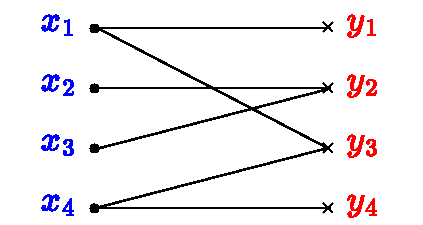
\includegraphics[width=0.35\textwidth,keepaspectratio]{Chapitre1/figures/correspondance.pdf}
  \caption{Example of correspondance $R$ between two sets $X = \{x_1, x_2, x_3, x_4\}$ and
  $Y = \{y_1, y_2, y_3, y_4 \}$. Here,
  $R = \{(x_1, y_1), (x_1, y_3), (x_2, y_2), (x_3, y_2), (x_4, y_3), (x_4, y_4) \}$.}
  \label{fig:correspondance}
\end{figure}
Denote $\mathcal R(X,Y)$ the collection of all correspondances between $X$ and $Y$,
then by Proposition 2.1 in \citep{Memoli11}, we have
\begin{equation} \label{haus_corres}
  d_{H}^{(Z, d)}(X,Y) = \inf_{R \in  \mathcal R(X,Y)} \sup_{(x,y) \in R} d(x,y)
  = \inf_{R \in \mathcal R(X,Y)} \vert\vert d \vert\vert_{L^{\infty}(R)}.
\end{equation}
Suppose that we equip each compact subset in $\cC(Z)$ with a Borel probability measure and consider
the collection of such "weighted spaces"
$\cC_w(Z) := \{(X,\mu_X): \text{supp}(\mu_X) = X \text{ and } X \in \cC(Z) \}$.
Given the similarity discussed above,
one can replace the correspondance by the admissible coupling and obtain the Wasserstein distance
\begin{equation}
  W_{Z, \infty}\big((X,\mu_X), (Y,\mu_Y) \big) :=
  \inf_{\pi \in U(\mu_X, \mu_Y)} \sup_{(x,y) \in R(\pi)} d(x,y)
  = \inf_{\pi \in U(\mu_X, \mu_Y)} \vert\vert d \vert\vert_{L^{\infty}(R(\pi))},
\end{equation}
where $R(\pi) := \text{supp}(\pi)$ the support of the measure $\pi$. Note that,
by Lemma 2.2 in \citep{Memoli11}, for any $\pi \in U(\mu_X, \mu_Y)$, we have
$R(\pi) \in  \mathcal R(\text{supp}(\mu_X), \text{supp}(\mu_Y))$, thus
$d_{H}^{(Z, d)} \leq W_{Z, \infty}$. By replacing the supremum norm with the $L^p$-norm,
we recover the $p$-Wasserstein distance
\begin{align}
    W_{Z, p}\big( (X,\mu_X), (Y,\mu_Y) \big)
    = \inf_{\pi \in U(\mu_X, \mu_Y)} \vert\vert d \vert\vert_{L^p(X \times Y, \pi)}.
\end{align}
To conclude, Diagram \eqref{fig:wass_motiv} summarizes
the process of transforming the Hausdorff distance into the $p$-Wasserstein distance,
when the compact metric space is equipped with a probability measure.
As we will see in \Cref{sec:gw}, this process is particularly useful
when extending to the setting of metric measure space.
\begin{figure}[ht]
  \centering
  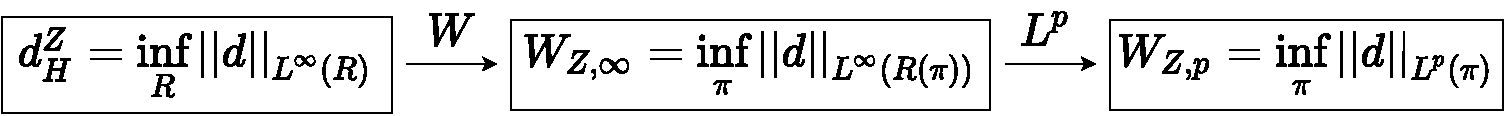
\includegraphics[width=0.85\textwidth,keepaspectratio]{Chapitre1/figures/wass_motiv.pdf}
  \caption{"W" indicates the \textit{Wassersteinization} process: replacing the optimization over the correspondances by over the admissible couplings.
  "$L^p$" indicates the \textit{$L^p$-ization} process: replacing the supremum norm by the $L^p$-norm.}
  \label{fig:wass_motiv}
\end{figure}
\subsubsection{Theory}
Since the seminal work of Kantorovich \citep{Kanto42},
the theory of OT has been profoundly developped in the last decades.
Different theoretical aspects with different level of generality
(from compact metric space to Polish space) are covered in various excellent references,
to name just a few, \citep{Villani03,Villani08,Fillipo15,Ambrosio05}. This list is
by no means exhaustive or representative. In this thesis, we only present a few
basic and useful properties of OT, which have much impact in machine learning.

\paragraph{Existence of solution, metric and weak convergence properties}
The existence of minimizer of the Kantorovich problem is guaranteed,
for example when the cost is lower semi-continuous and bounded below
(Theorem 4.1 in \citep{Villani08}). Note that,
apart from the classic choice of cost function $c = d^p$ as in the Wasserstein distance,
there are other alternatives, for example, the Bregman divergence \citep{Guo21},
or even the Wasserstein distance \citep{Huizing22}.

The Wasserstein distance defines a metric
on the space of probability measures with finite moments of order $p \geq 1$
(Theorem 7.3 in \citep{Villani03}) and characterizes the weak convergence: for any $p \geq 1$,
we have $\mu_n \rightharpoonup \mu$ if and only if $W_p(\mu_n, \mu) \to 0$
(Theorem 7.12 in \citep{Villani03}).
This topological property also holds for the integral probability metric \citep{Muller97},
but not for other popular statistical divergences, namely the Kullback-Leibler divergence,
total variation, Hellinger distance
\footnote{More detailed comparison amongst divergences can be found in \citep{Gibbs02}.}.

\paragraph{Duality theory}
Given the convexity of the OT problem, another very powerful property
is the duality theorem, which asserts that the strong duality holds. More precisely,
if $X, Y$ are compact metric spaces and the cost $c$ is continuous, then by Theorem 1.46
in \citep{Fillipo15}, one has
\begin{align*}
  \ot(\mu, \nu) = \sup_{\substack{(f, g) \in \cC_b(X) \times \cC_b(Y) \\ f \oplus g \leq c}} \;
  \int_X f d\mu + \int_Y g d\nu
\end{align*}
where $\cC_b(X), \cC_b(Y)$ denote the space of bounded continuous functions on $X, Y$, respectively.
Strong duality still holds in a much more general setting (see Theorem 5.10 in \citep{Villani08}).
The theory of duality plays a crucial role, not only in theoritical study, but also
in practical applications. In particular, it is at the heart of some exact solvers
for the discrete OT problem (see Section 3 in \citep{Peyre19}).
In the case of Wasserstein distance, the duality theory allows to deduce other reformulations
of the primal problem, which have recently attracted much interest in machine learning.
We now discuss two particular important applications.

\paragraph{$2$-Wasserstein distance}
Under mild assumptions on the probability measures, thanks to the duality and
Brenier's theorems \citep{Brenier87}, Theorem 2.9 in \citep{Villani03} states that
the $2$-Wasserstein distance can be rewritten as the optimization of convex functions.
This result has been used to estimate the Wasserstein distance
\citep{Chartrand09,Taghvaei19,Korotin19,Makkuva20},
where the functional is parametrized by an input convex neural network \citep{Amos17}.

\paragraph{$1$-Wasserstein distance}
An important application of the duality theory is the $1$-Wasserstein distance
(also known as \textit{Earth mover's distance}). Its dual problem
\footnote{Also known as the \textit{Kantorovich-Rubinstein duality}, see Remark 6.5
in \citep{Villani08}. More discussion on the $1$-Wasserstein distance can be found
in Chapter 6 in \citep{Peyre19}.}
is a reformulation of the primal problem as the maximization over all $1$-Lipschitz functionals,
which can be parametrized by neural networks.
In practice, the the $1$-Wasserstein distance has been successfully used
in the training of generative adversarial networks (GAN) \citep{Goodfellow14},
thanks to the seminal work of \citep{Arjovsky17} on Wasserstein GAN (WGAN).
There have been various extensions and improvements of WGAN, for example
smoothed WGAN \citep{Sanjabi18}, WGAN-GP \citep{Gulrajani17}, WGAN-LP \citep{Petzka18},
Sobolev-GAN \citep{Mroueh17}. It is also the motivation for other OT-based GAN methods, namely
Sinkhorn divergence-GAN \citep{Genevay18a}, OT-GAN \citep{Salimans18}.
Interestingly, WGAN also finds its connections with the Minkowski and Alexandrov problems
in convex geometry \citep{Lei19}, and with the soft-margin formulation of
Support Vector Machine \citep{Jolicoeur19}.

\subsubsection{Approximation and algorithm}
In discrete setting, the OT formulation is a linear program.
An example of exact solver \footnote{See also Chapter 3 in \citep{Peyre19}
for a more detailed discussion on classic algorithms and Section 2.1 in \citep{Pele09}
for an overview on computational complexity.}
is the interior point method \citep{Orlin88}. It requires the complexity of $O(n^3 \log n)$,
which is computationally prohibitive in many applications.
There exist some approaches to overcome this limitation. For example, the mini-batch approach
\citep{Sommerfeld19,Fatras20} considers multiple resamplings of the data and
uses the average of distances computed in the mini-batches as an estimation of the true OT distance.
The "sliced" method \citep{Rabin12,Bonneel15} develops an alternative metric
called \textit{Sliced Wasserstein distance}.
It relies on the fact that computing the $1$-D Wasserstein distance boils down to sorting the
point values, which only requires the complexity of $O(n \log n)$.
Using the framework from statistical physics, \citep{Koehl19}
approximate the OT distance by the free energy evaluated at sufficiently small temperature.
From a more mathematical viewpoint, this idea is based on the interesting relation
between the minimum and the logsumexp operation, where informally, one has that:
$\min f(x) = \lim_{\beta \to 0^+} -\frac{1}{\beta} \int e^{-\beta f(x)} dx$.

\paragraph{Entropic OT problem}
In this thesis, we focus on the line of works on the discrete entropic approximation
\footnote{For a mathematical introduction in the general setting,
interested readers may consult the lecture note of \citep{Nutz22}.} defined by:
for $\varepsilon > 0$,
\begin{align}
  \label{eq:primal_ot}
  \ot_{\varepsilon}(\mu, \nu) = \inf_{P \in U(\mu, \nu)} \langle C, P \rangle +
  \varepsilon \; \kl(P | \mu \otimes \nu).
\end{align}
In the OT literature, the entropic regularization can sometimes be referred to the case where
the regularizer is the negative entropy defined by $H(P) = \sum_{i,j} P_{ij} (\log P_{ij} - 1)$.
However, since $\kl(P | \mu \otimes \nu) = H(P) - H(\mu) - H(\nu)$, for any $P \in U(\mu, \nu)$,
the two regularized problems are equivalent, up to a constant.
Interestingly, the entropic OT is an even older problem than the unregularized one.
It was already studied in the early 30's by \citep{Schrodinger32},
under the name \textit{static Schrodinger bridge problem}.
The entropic OT problem has attracted much attention to the
machine learning community thanks to the seminal work of \citep{Cuturi13}.

Note that, the entropic regularization introduces bias,
in the sense that $\ot_{\varepsilon}(\mu, \mu) \neq 0$, for any $\varepsilon > 0$.
This issue can be easily overcome by considering the Sinkhorn divergence
\footnote{This divergence is implemented very efficiently in the Geomloss package \citep{Feydy19}.}
\citep{Ramdas17,Feydy19} defined by
\begin{align*}
  \text{SD}_{\varepsilon}(\mu, \nu) = \ot_{\varepsilon}(\mu, \nu)
  - \frac{1}{2} \left[ \ot_{\varepsilon}(\mu, \mu) + \ot_{\varepsilon}(\nu, \nu) \right]
\end{align*}
Not only being unbiased, the Sinkhorn divergence also enjoys favorable topological, statistical
and interpolation properties \citep{Feydy19,Genevay19}. In particular,
if the cost is the squared $l_2$-norm, then it is a good proxy
for the squared $2$-Wasserstein distance. More precisely, under mild conditions on $\mu$ and $\nu$,
one has that $| \text{SD}_{\varepsilon}(\mu, \nu) - W_2^2(\mu, \nu) | = O(\varepsilon^2)$
\citep{Chizat20}.

\paragraph{Properties} The entropic OT has many interesting properties. First, it is a
good and scalable approximation of OT distance,
where the approximation error can be quantified in some settings \citep{Genevay19,Luise18}.
Moreover, the convergence behaviors of minima and minimizer are also well understood
\citep{Leonard12,Carlier17} and the convergence rate exists in some practical situations
\citep{Genevay19,Cominetti94,Weed18}.
Second, since entropic OT is a convex problem, strong duality holds and one has that
\begin{align}
  \label{eq:dual_ot}
  \ot_{\varepsilon}(\mu, \nu) = \sup_{\substack{f \in \bbR^m \\ g \in \bbR^n}}
  \langle f, \mu \rangle + \langle g, \nu \rangle
  - \varepsilon \; \left\langle \exp \left( \frac{f \oplus g - C}{\varepsilon} \right), \mu \otimes \nu \right\rangle
\end{align}
Arguably, this is the most important premise in the study of the entropic approximation, which
allows to develop and analyze many Sinkhorn-based algorithms (see \Cref{para:summary} for discussion).
In particular, \citep{Genevay19} use the dual problem to show that entropic OT
has better sample complexity than unregularized OT,
though it fixes the bottleneck in the sample size by introducing a new one in the regularization.
This issue can be mitigated, for example when the probability measures are sub-Gaussian \citep{Mena19}.
Entropic OT is also known for its joint convexity, smoothness with respect to
the inputs \citep{Luise18} and metric property \citep{Sanjabi18}.

\paragraph{Algorithm} To solve the dual problem \ref{eq:dual_ot},
we are interested in the deterministic approach, where the most popular solver
is the Sinkhorn algorithm \citep{Sinkhorn67}
\footnote{Also known as \textit{matrix scaling algorithm}.
For the historical perspective, see Remark 4.5 in \citep{Peyre19}.}.
Denote $K = e^{-C / \varepsilon}$ the kernel matrix. Then,
from the first-order optimality conditions of the dual problem, the iterates read
\begin{align}
  u^{(t+1)} = \frac{\mu}{Kv^{(t)}} \text{ and } v^{(t+1)} = \frac{\nu}{K^T u^{(t+1)}}.
\end{align}
This algorithm is very easy to implement and available in the Python Optimal Transport
\citep{Flamary21} and OTT-JAX \citep{Cuturi22} packages.
It is well known that it converges globally to the optimal dual vectors of the dual problem
\citep{Sinkhorn67}, at a linear rate in variation semi-norm \citep{Franklin89}.
The OT plan then can be retrieved from the optimal solution $(u, v)$ by
$P = (\mu \otimes \nu) \odot (u \otimes v) \odot K$,
where $\otimes$ is the element-wise multiplication.

% Note that, as Sinkhorn algorithm is nothing but a coordinate ascent algorithm,
% \footnote{Note that the "one-at-a-time" scheme must be used
% (\ie $u^{(t+1)}$ is used in the calculation of $v^{(t+1)}$), whereas the "all-at-once" scheme
% (\ie $u^{(t)}$ is used in the calculation of $v^{(t+1)}$) does not necessarily guarantee the convergence.
% See, for example \url{https://www.stat.cmu.edu/~ryantibs/convexopt-F16/scribes/coord-desc-scribed.pdf}.}

\paragraph{Discussion on Sinkhorn algorithm}
The Sinkhorn algorithm has two key advantages. First, since the iterates only require
vector-matrix multiplication, they can be seamlessly parallerized.
One can further speed up the computation by exploiting the structure of the kernel matrix
(see Section 4.3 in \citep{Peyre19}). Second, it is enough to store only the dual vectors
(which cost $O(n)$ in memory) because the OT plan (which costs $O(n^2)$ in memory)
can be easily queried on demand.

However, the smaller the regularization, the more it hurts the Sinkhorn algorithm.
First, if the number of iterations is not sufficiently large,
the algorithm may fail to converge and the resulting transport plan can be inadmissible.
To circumvent this issue, one can apply the rounding algorithm \citep{Altschuler17},
which adjusts the coordinates of the coupling matrix until the marginal constraints are met.
While being admissible, the rounded transport plan may not be the solution of the entropic OT problem.

Second, when $\varepsilon$ is close to $0$, the quick saturation of the kernel
$\exp^{-C / \varepsilon}$ to the zero matrix may trigger the numerical error caused by the division by zero.
To avoid this numerical instability, the implementation in the log-domain is recommended
at the cost of slowing down the algorithm, due to the logsumexp operation.
More precisely, the log-domain iterates read
\begin{enumerate}
  \item $f^{(t+1)} = \log \mu - \log \sum_j \exp \left( g_j^{(t)} - \frac{C_{\cdot, j}}{\varepsilon} \right)$.
  \item $g^{(t+1)} = \log \nu - \log \sum_i \exp \left( f_i^{(t+1)} - \frac{C_{i, \cdot}}{\varepsilon} \right)$.
\end{enumerate}
To mitigate the side effect, one can use the redundant parametrization strategy
\citep{Chizat18a,Schmitzer19}, which additionally performs "absorption" iterations
to reduce the computational overhead of the logsumexp operation.

Third, the initialization of dual vectors is important.
Under the absence of prior knowledge, the most popular practice is to initialize with
the zero vectors, which usually leads to poor convergence behavior for very small regularization.
One can use the $\varepsilon$-scaling scheme \citep{Schmitzer19}
\footnote{This strategy is very efficiently exploited and implemented in the Geomloss package
\citep{Feydy19}}, whose idea is simple: we fix a decreasing sequence of regularizations
converging to $\varepsilon$, then successively use the solution of the previous problem to
initialize the next one. However, this can be very costly due to the amount of subproblems,
while not necessarily ensuring the convergence to the true minimizer of the entropic OT problem.
Recently, \citep{Thornton23a} leverage the fact that the dual vectors in unregularized OT problem
can admit closed-form expressions for $1$D-OT and Gaussian measures, and propose to use them
as initialization. They empirically show that, this practice can result in much less iterations,
thus significantly speed up and improve the convergence of the Sinkhorn algorithm.

\paragraph{Summary} \label{para:summary}
We conclude the discussion on balanced OT with some remarks.
First, despite the prohibitive theoretical complexity,
efficient implementation of exact solver for unregularized OT exists \citep{Flamary21},
and can work well on datasets of size up to $O(10^4)$.

Second, it is also possible to directly estimate the OT distance using the
Bregman proximal point method \citep{Chen93,Teboulle97}, where for fixed learning rate $\eta > 0$,
at iteration $t$, we solve
\begin{align}
  \label{eq:bpp_eot}
  P^{(t+1)} = \argmin_{P \in U(\mu, \nu)} \langle C, P \rangle + \eta \; \kl(P, P^{(t)}).
\end{align}
This is a slightly modified entropic OT problem and can still be solved with the
Sinkhorn algorithm, but now the OT plan is computed by
\begin{align*}
  P^{(t+1)} = P^{(t)} \odot \exp \left( \frac{f^{(t+1)} \oplus g^{(t+1)} - C}{\eta} \right),
\end{align*}
where $(f^{(t+1)}, g^{(t+1)})$ is the optimal dual vectors of the problem \ref{eq:bpp_eot}.
Classic results \citep{Chen93} guarantee the linear convergence of BPP method
to the minimum and the minimizer of the OT problem.
Interestingly, it is not necessarily to solve \textbf{exactly} the entropic problem \ref{eq:bpp_eot},
but even as few as one Sinkhorn iteration can work in practice.
This approach, known as \textit{Inexact Proximal OT} (IPOT), is introduced in \citep{Xie20}.
Later, we will see in \Cref{sec:input} that it can be easily extended to the unbalanced OT setting
and achieves superior performance to other existing methods.

Third, the recent improvements on the Sinkhorn algorithm,
namely the over-relaxation method \citep{Lehmann21,Thibault21}, the screening strategy \citep{Alaya19},
or the greedy approach \citep{Altschuler17,Lin20,Kostic21}, usually focus on careful elaboration
of the iterates. There are also gradient-based solvers for the entropic OT, notably
the adaptive primal-dual accelerated mirror descent \citep{Dvurechensky18,Lin22},
or the stochastic gradient descent \citep{Abid18,Genevay16,Seguy18}.

Last, while entropy is the most popular and well-studied regularizer,
there exist other alternatives summarized in \Cref{t:ot_variation}, which aim to
integrate the prior knowledge on the data, or the structure of the transport matrix.
\begin{table}[t]
	\centering
		\begin{tabular}{|l|l|}
    \hline
    \textbf{Regularizer} & \textbf{Reference} \\
    \hline
    Convex regularizer & \citep{Marino20b} \\
    \hline
    \makecell[l]{Strongly convex regularizer \\ (negative entropy, square $2$-norm, group lasso)}
    & \makecell[l]{\citep{Dessein16} \\ \citep{Blondel18}} \\
    \hline
    \makecell[l]{Class-based regularizer \\ (group lasso, Laplacian)} & \citep{Courty16} \\
    \hline
    \makecell[l]{Sparse-promoting regularizer \\ (group lasso, weighted $1$-norm)}
    & \makecell[l]{\citep{Lindback23}} \\
    \hline
    Sparsity-constraint regularizer & \citep{Liu22} \\
    \hline
    Csiszár divergence & \citep{terjek22} \\
    \hline
    Square $2$-norm & \makecell[l]{\citep{Roberts17} \\ \citep{Blondel18} \\ \citep{Lorenz21}} \\
    \hline
    Tsallis $q$-entropy & \citep{Muzellec17} \\
    \hline
    Deformed $q$-entropy & \citep{Bao22} \\
    \hline
    \end{tabular}
		\caption{Classes of regularizers in regularized OT problem. \label{t:ot_variation}}
\end{table}

%%%%%%%%%%%%%%%%%%%%
\subsection{Unbalanced Optimal Transport}

\subsubsection{Formulation and properties}

Recall that the balanced OT enforces hard constraints on the marginal distributions
of the OT plan. These constraints lead to two main disadvantages. First,
imbalanced datasets where samples are re-weighted cannot be accurately compared.
Second, mass transportation must be exhaustive in the sense that,
outliers, if any, must be matched regardless of the cost they induce.

To circumvent these limitations, a straightforward solution is to control
the difference between the marginal distributions of the transportation plan
and the data by some discrepancy measure. This gives rise to the unbalanced OT (UOT),
which was first proposed by \citep{Benamou03}.
The theoretical and numerical aspects of this relaxation
have been studied extensively \citep{Liero18,Chizat18b,Chizat18a,Khiem20}
and have been gaining increasing attention in the machine learning community,
with wide-range applications, namely in domain adaptation \citep{Fatras21},
generative adversarial networks \citep{Balaji20, Yang19}, dynamic tracking \citep{Lee19},
crowd counting \citep{Ma21}, neuroscience \citep{janati2019group, bazeille2019} or
modeling cell developmental trajectories \citep{Schiebinger19}.
Unbalanced OT and its variants are usually sought for
their known robustness to outliers \citep{Mukherjee21,Balaji20,Fatras21,Nietert22,Le21}.

\paragraph{Formulation} To define the UOT problem, let us start with
the Csiszár divergence \citep{Csiszar63}. Given an entropy function
$\varphi : \mathbb R_{> 0} \to [0, \infty]$ (\textit{i.e.} it is convex,
positive and lower semi-continuous such that $\varphi(1) = 0$), we define
the recession constant $\varphi_{\infty}' \in \mathbb R \cup \{ \infty \}$ as
\begin{equation}
  \varphi_{\infty}' = \lim_{x \to \infty} \frac{\varphi(x)}{x}.
\end{equation}
Denote $\mathcal M^+(\mathcal S)$ the set of finite nonnegative Radon measures on a
Hausdorff topological space $S$. The Csiszár divergence (or $\varphi$-divergence) between
two measures $\mu$ and $\nu$ in $\mathcal M^+(\mathcal S)$ is defined as
\begin{equation}
  D_{\varphi}(\mu \vert \nu) = \int_\mathcal S \varphi \Big( \frac{d\mu}{d\nu} \Big) d\nu +
  \varphi_{\infty}' \int_\mathcal S d\mu^{\perp},
\end{equation}
where, by Lebesgue decomposition, we have $\mu = \frac{d\mu}{d\nu} \nu + \mu^{\perp}$.
It is jointly convex, positive and weakly lower-semicontinuous \citep{Liero18}.
The analysis of some Csiszár divergences can be found in \citep{Sejourne19}.
Here, we are mostly interested in two following special cases:
\begin{itemize}
  \item[$\bullet$] The Kullback-Leibler (KL) divergence defined by
  \begin{equation}
    \kl(\mu \vert \nu) =
    \begin{cases}
      \int \frac{d \mu}{ d \nu} \log \frac{d \mu}{ d \nu} - \int d\mu + \int d\nu,
      \text{ if } \mu \ll \nu \\
      \infty, \text{ otherwise}.
    \end{cases}
  \end{equation}
  corresponds to $\varphi(x) = x \log x - x + 1$.

  \item[$\bullet$] The indicator divergence $\iota_{=}(\mu \vert \nu)$ is equal to $0$
  if $\mu = \nu$ and $+\infty$ otherwise.
  Its entropy function is $\varphi = \iota_{\{ 1 \}}$, where the indicator function $\iota_C$
  of a convex set $C$ is defined by $\iota_C(x)$ is equal to $0$ if $x\in C$ and $+\infty$ otherwise.
  This divergence results in the balanced OT.
\end{itemize}
Given a proper lower semicontinuous cost function $c: X \times Y \to [0, \infty]$
and for $\rho_1, \rho_2 \geq 0$, the UOT cost between two measures $\mu \in \cM^+(X)$ and
$\nu \in \cM^+(Y)$ is defined by
\begin{align*}
  \uot_{\rho}(\mu, \nu) = \inf_{\pi \in \cM^+(X \times Y)} \int c \; d\pi
  + \rho_1 D_{\varphi_1}(\pi_{\# 1} | \mu)
  + \rho_2 D_{\varphi_2}(\pi_{\# 2} | \nu)
\end{align*}

\paragraph{Properties} Under mild conditions of the cost and entropy functions,
the UOT problem always admits a solution (Theorem 3.3 in \citep{Liero18}).
Similar to the balanced case, UOT also enjoys the metric properties, duality theory and
dynamic formulation, to name a few. For a more complete treatment on the theory of UOT,
readers are invited to see the seminal works of \citep{Liero18,Chizat18b}, and the reference therein.
The case where $D_{\varphi_1} = D_{\varphi_2} = \kl$ is also of our special interest,
since it allows to show that the UOT is robust to outliers.
\begin{proposition}[Generalization of Lemma 1 in \citep{Fatras21}]
  Let $\mu, \mu_o$ be two nonnegative finite Borel measures with disjoint compact supports $E, E_o$,
  respectively. For $\alpha \in [0, 1]$, denote $\widetilde{\mu} = \alpha \mu + (1 - \alpha) \mu_o$
  the noisy measure. Then, for any nonnegative finite Borel measures $\nu$
  with compact support $F$, we have
  \begin{align}
    \label{eq:ot_robust}
    \ot(\widetilde{\mu}, \nu) \geq
    (1 - \alpha) \inf_{(x, y) \in E_o \times F} c(x, y),
  \end{align}
  whereas
  \begin{align}
    \uot_{\rho}(\widetilde{\mu}, \nu) \leq \alpha \uot_{\rho}(\mu, \nu) +
    (1 - \alpha) M
    \left( 1 - \exp \left( -\frac{K}{M} \right) \right)
  \end{align}
  where, $K = \int c(x, y) \; d\mu_o(x) d\nu(y)$ and $M = \rho_1 m(\mu_o) + \rho_2 m(\nu)$.
  Here, $m(\mu)$ denotes the mass of measure $\mu$.
\end{proposition}
Clearly, the behavior of the outliers is always controlled in UOT.
Thanks to the marginal relaxation, if the outlier is too impactful,
its impact will quickly saturate to $0$, meaning that it receives no mass from other points.
By contrast, this is not the case for balanced OT, since every point (including outliers)
must be aligned regardless of its cost, due to the marginal constraints. The right-hand side of
the inequality \ref{eq:ot_robust} can be made arbitrarily large by taking outliers "far" enough
from the clean data.

\subsubsection{Optimization and algorithm} \label{sub:uot_optim}

In general, given any differentiable divergence and regularizer, since Problem \ref{eq:generic_uot}
is a bound-constrained minimization problem, it can be solved with the L-BFGS-B algorithm
\citep{Byrd95,Zhu97}. When $D_{\varphi_1} = D_{\varphi_2} = \kl$, the unregularized UOT can
be approximated with entropic regularization. The main advantages of this approach include
well-understood convergence analysis \citep{Chizat18a}, statistical properties \citep{Sejourne19},
GPU-friendly implementation, strong convexity and smoothness coming from the dual problem,
making it a suitable training loss for neural networks.
While entropic regularization also introduces bias to the UOT, it is possible to debiase
using the same trick as in the balanced counterpart \citep{Sejourne19}.

It is important to note that, in the OT literature, the entropic regularization
can be referred to two different regularizers: the negative entropy \citep{Frogner15, Chizat18a} and
the KL divergence \citep{Sejourne19}. We cover both cases by considering a
more general formulation: given the hyperparameters
$\rho_1, \rho_2 \geq 0, \varepsilon > 0$, the cost matrix $C \in \bbR^{m \times n}$
and the positive measures $\mu \in \bbR^m_{> 0}, \nu \in \bbR^n{> 0}, \gamma \in \bbR^{m \times n}_{> 0}$,
we want to solve the problem
\begin{align}
  \label{eq:discrete_ent_uot}
  \uot_{\varepsilon, \rho} = \min_{P \in \bbR^{m \times n}_{\geq 0}} \langle C, P \rangle + \rho_1 \kl(P_{\# 1} | \mu)
  + \rho_2 \kl(P_{\# 2} | \nu) + \varepsilon \kl(P | \gamma).
\end{align}
Denote $m(Q) = \sum_{i, j} Q_{ij}$ the mass of measure $Q$. Observe that
\begin{align}
  \langle C, P \rangle + \varepsilon \kl(P | \gamma) &=
  \varepsilon \left[ \sum_{i, j} P_{ij} \log P_{ij} -
  \sum_{i, j} P_{ij} \left( \log \gamma_{ij} - \frac{C_{ij}}{\varepsilon} \right)
  - \sum_{i, j} P_{ij} + \sum_{i, j} \gamma_{ij} \right] \\
  &= \varepsilon \kl \left(P \Big| \exp \left( -\frac{C - \log \gamma}{\varepsilon} \right) \right)
  + \varepsilon \left[ m(\gamma) - m \big(\gamma \odot e^{-C / \varepsilon} \big) \right],
\end{align}
where $\odot$ is the element-wise multiplication between two matrices and the exponential operation
is also element-wise. Now, the ambiguity of the entropic regularizer is naturally handled in
Problem \ref{eq:discrete_ent_uot}. More precisely,
the KL divergence corresponds to $\gamma = \mu \otimes \nu$ whereas
the negative entropy corresponds to $\gamma = 1_{m \times n}$,
since $\kl(P | 1_{m \times n}) = \langle P, \log P \rangle - m(P) + mn = H(P) + mn$.

An interesting property of Problem \ref{eq:discrete_ent_uot}, which does not exist in the
balanced OT or for other Csiszár divergences,
is that the minimum can be explicitly expressed as a function of minimizer.
This proves to be particularly helpful when studying the computational complexity of
Sinkhorn algorithm \citep{Khiem20}.
\begin{lemma}[Slight generalization of Lemma 4 in \citep{Khiem20}]
  \label{eq:uot_minimizer}
Denote $P^*$ is the minimizer of Problem \ref{eq:discrete_ent_uot}. Then,
\begin{align*}
  \uot_{\varepsilon, \rho} = \rho_1 m(\mu) + \rho_2 m(\nu) + \varepsilon m(\gamma)
  - (\rho_1 + \rho_2 + \varepsilon) \; m(P^*)
\end{align*}
\end{lemma}
While trivial, we remark that, \Cref{eq:uot_minimizer} holds for unregularized UOT
(\textit{i.e.} $\varepsilon = 0$). Later, we will see how this result can also be extended
to other unbalanced divergences, namely the unbalanced Gromov-Wasserstein and
unbalanced Co-Optimal Transport.
Now, we discuss some existing approaches to Problem \ref{eq:discrete_ent_uot}.

\paragraph{Sinkhorn algorithm} The Sinkhorn algorithm can be extended easily to the entropic UOT.
\footnote{When the regularizer is the negative entropy, the Sinkhorn algorithm is also called
\textit{scaling algorithm} \citep{Chizat18a}.} The (strict) convexity of the primal problem ensures
that duality holds, thanks to the Fenchel-Rockafellar duality theorem. In particular,
The dual problem of Problem \ref{eq:discrete_ent_uot} reads
\begin{align}
  \label{eq:dual_uot}
  \sup_{\substack{f \in \bbR^m \\ g \in \bbR^n}}
  -\rho_1 \; \left\langle \exp \left( - \frac{f}{\rho_1}\right), \mu \right\rangle
  -\rho_2 \; \left\langle \exp \left( - \frac{g}{\rho_2} \right), \nu \right\rangle
  - \varepsilon \; \left\langle \exp \left( \frac{f \oplus g - C}{\varepsilon} \right), \gamma \right\rangle
\end{align}
Similar to the balanced case, the OT plan can be retrieved from the optimal solution $(f^*, g^*)$ by
\begin{align*}
  P^* = \gamma \odot \exp \left( \frac{f^* \oplus g^* - C}{\varepsilon} \right)
\end{align*}
Note that, when $\rho_1, \rho_2 \to \infty$, we have
$-\rho_1 \; \left\langle \exp \left( - \frac{f}{\rho_1}\right), \mu \right\rangle \to
\langle f, \mu \rangle$ and
$-\rho_2 \; \left\langle \exp \left( - \frac{g}{\rho_2} \right), \nu \right\rangle \to \langle g, \mu \rangle$.
So, we recover the dual problem of the entropic balanced OT.
When $\varepsilon \to 0$, we have
$\varepsilon \; \left\langle \exp \left( \frac{f \oplus g - C}{\varepsilon} \right), \gamma \right\rangle$
converges to the constraint $f \oplus g \leq C$, which corresponds to the dual problem of the
unregularized UOT problem.

Similar to the balanced case, the log-domain Sinkhorn algorithm \ref{alg:Sinkhorn_algo}
applied to the dual problem \ref{eq:dual_uot} consists in alternatively updating the dual vectors.
Here, the generalized softmin operator is defined by
$\overline{\smin}^{\nu_j, \gamma_{\cdot, j}}_{\varepsilon}(f) =
\varepsilon \left( \log \nu_j - \log \langle \gamma_{\cdot, j}, e^{-f / \varepsilon} \rangle \right)$,
for $j \in [n]$. In particular, when $\gamma = \mu \otimes \nu$, we recover the softmin operator
\citep{Sejourne19} defined by
$\smin^{\mu}_{\varepsilon}(f) = -\varepsilon \log \langle \mu, e^{-f / \varepsilon} \rangle$.
More generally, the Sinkhorn algorithm is applicable to all Csiszár divergences,
as long as the regularizer is the KL divergence (see Definition 3 in \citep{Sejourne19}).
We leave the convergence analysis to the discussion of the next method.
In practice, the Sinkhorn algorithm also suffers from slow convergence for small regularization
and can be accelerated using the similar workarounds in the balanced setting.

\begin{algorithm}[t]
  \caption{Sinkhorn algorithm for Problem \ref{eq:discrete_ent_uot}.}
  \label{alg:Sinkhorn_algo}
\begin{algorithmic}[1]
  \STATE \textbf{Input:} cost matrix $C \in \bbR^{m \times n}$,
  measures $\mu \in \bbR^m_{> 0}, \nu \in \bbR^n_{> 0}, \gamma \in \bbR^{m \times n}_{> 0}$,
  regularization $\varepsilon > 0$, relaxation parameters $\rho_1, \rho_2 > 0$.
  \FOR{$t=1, \dots, T$}
  \STATE $f_i^{(t+1)} \gets \frac{\rho_1}{\rho_1 + \varepsilon} \; \overline{\smin}^{\mu_i, \gamma_{i, \cdot}}_{\varepsilon}(C_{i, \cdot} - g^{(t)})$, for $i \in [m]$.
  \STATE $g_j^{(t+1)} \gets \frac{\rho_2}{\rho_2 + \varepsilon} \; \overline{\smin}^{\nu_j, \gamma_{\cdot, j}}_{\varepsilon}(C_{\cdot, j} - f^{(t+1)})$, for $j \in [n]$.
  \ENDFOR
  \STATE \textbf{Output:} pair of dual vectors $(f^{(T)}, g^{(T)})$.
\end{algorithmic}
\end{algorithm}

\paragraph{Translation Invariant Sinkhorn (TI-Sinkhorn)} Recall that, in the entropic balanced OT,
due to the linear structure in the objective function of the dual problem,
if $(f, g)$ is the optimal solution, then so is $(f + \lambda, g - \lambda)$,
for every $\lambda \in \bbR$. However, this translation invariant (TI) property no longer holds for
the unbalanced counterpart. As observed in \citep{Sejourne21}, this is problematic because
the convergence of dual vectors depends on the translation (since the iterates do),
thus is sensitive to initialization. Moreover, it becomes very slow when the regularization
is too small relative to the relaxation ($\varepsilon \ll \rho$).
This issue can be mitigated by considering the optimization problem
\begin{align}
  H_{\varepsilon}(\overline{f}, \overline{g}) := \sup_{\lambda \in \bbR}
  F_{\varepsilon}(\overline{f} + \lambda, \overline{g} - \lambda)
\end{align}
where $F_{\varepsilon}$ is the objective function of the dual problem \ref{eq:dual_uot}.
By Proposition 2 in \citep{Sejourne21}, the optimality happens when
\begin{align}
  \label{eq:optimal_lambda}
  \lambda^*(\overline{f}, \overline{g}) = \frac{\rho_1 \rho_2}{\rho_1 + \rho_2}
  \log \frac{\langle \mu, e^{-\overline{f} / \rho_1} \rangle}{\langle \nu, e^{-\overline{g} / \rho_2} \rangle}.
\end{align}
By construction, $H_{\varepsilon}$ is TI. Not only $H_{\varepsilon}$ and $F_{\varepsilon}$
have the same maximum, but also the their maximizers are related by the equation
$(f, g) = (\overline{f} + \lambda^*(\overline{f}, \overline{g}), \overline{g} - \lambda^*(\overline{f}, \overline{g}))$.
The details of the TI-Sinkhorn algorithm applied to Problem \ref{eq:discrete_ent_uot}
can be found in \Cref{alg:TI_Sinkhorn}.

To analyze the convergence of TI-Sinkhorn, we introduce two norms:
the supremum norm $||f||_{\infty} = \max_i | f_i|$ and the
Hilber pseudo-norm $||f||_* = \frac{1}{2} \left( \max_i f_i - \min_i f_i \right)$.
Denote $\kappa_{\varepsilon}(\mu)$ the contraction rate of the softmin operator
$\smin_{\varepsilon}^{\mu}$ for the norm $||f||_*$, meaning that
\begin{align}
  ||\smin_{\varepsilon}^{\mu}(C - f_1) - \smin_{\varepsilon}^{\mu}(C - f_2) ||_* \leq
  \kappa_{\varepsilon}(\mu) \; || f_1 - f_2 ||_*
\end{align}
The convergence of Sinkhorn and TI-Sinkhorn algorithms when $\gamma = \mu \otimes \nu$
is summarized in the following result.
\begin{proposition}
  [Theorem 1 in \citep{Sejourne21}] Denote $(f^*, g^*)$ the optimal solution of
  the dual problem \ref{eq:dual_uot}. Given initialization $f_0$, suppose
  $(f_t, g_t), (\overline{f}_t, \overline{g}_t)$ are the iterates
  of the Sinkhorn and TI-Sinkhorn algorithms at iteration $t$, respectively. Denote
  $\kappa = \left( 1 + \frac{\varepsilon}{\rho_1} \right)^{-1} \left( 1 + \frac{\varepsilon}{\rho_2} \right)^{-1}$
  and $\overline{\kappa} = \kappa_{\varepsilon}(\mu) \kappa_{\varepsilon}(\nu) \kappa$. Then,
  for Sinkhorn algorithm, we have
  \begin{align}
    || f^{(t)} - f^* ||_{\infty} + || g^{(t)} - g^* ||_{\infty} \leq 2 \kappa^t || f^{(0)} - f^* ||_*.
  \end{align}
  whereas for TI-Sinkhorn algorithm,
  \begin{align}
    || \overline{f}^{(t)} - f^* ||_{\infty} + || \overline{g}^{(t)} - g^* ||_{\infty} \leq
    2 \overline{\kappa}^t || f^{(0)} - f^* ||_*.
  \end{align}
\end{proposition}
In other words, TI-Sinkhorn improves the convergence rate of Sinkhorn by a factor of
$\kappa_{\varepsilon}(\mu) \kappa_{\varepsilon}(\nu)$. However, when $\varepsilon \ll \rho$,
not only $\kappa \approx 1$, but also empirically
$\kappa_{\varepsilon}(\mu) \kappa_{\varepsilon}(\nu) \approx 1$.
For this reason, despite the acceleration over Sinkhorn,
TI-Sinkhorn still suffers from small regularization and remains slow in such situation.

\begin{algorithm}[t]
  \caption{TI-Sinkhorn algorithm for Problem \ref{eq:discrete_ent_uot}.}
  \label{alg:TI_Sinkhorn}
\begin{algorithmic}[1]
  \STATE \textbf{Input:} cost matrix $C \in \bbR^{m \times n}$,
  measures $\mu \in \bbR^m_{> 0}, \nu \in \bbR^n_{> 0}, \gamma \in \bbR^{m \times n}_{> 0}$,
  regularization $\varepsilon > 0$, relaxation parameters $\rho_1, \rho_2 > 0$.
  \STATE Calculate $k_{ij} = \frac{\varepsilon}{\varepsilon + \rho_i} \frac{\rho_j}{\rho_1 + \rho_2}$,
  for $i, j \in \{ 1, 2\}$, and $\xi_{ij} = \frac{k_{ij}}{1 - k_{ij}}$, for $i \neq j$.
  \FOR{$t=1, \dots, T$}
  \STATE $f_i \gets \frac{\rho_1}{\rho_1 + \varepsilon} \; \overline{\smin}^{\mu_i, \gamma_{i, \cdot}}_{\varepsilon}(C_{i, \cdot} - g^{(t)})
  - k_{11} \; \smin^{\nu}_{\rho_2}(g^{(t)})$, for $i \in [m]$.
  \STATE $f^{(t+1)} \gets f + \xi_{12} \; \smin^{\mu}_{\rho_1}(f)$.
  \STATE $g_j \gets \frac{\rho_2}{\rho_2 + \varepsilon} \; \overline{\smin}^{\nu_j, \gamma_{\cdot, j}}_{\varepsilon}(C_{\cdot, j} - f^{(t+1)})
  - k_{22} \; \smin^{\mu}_{\rho_1}(f^{(t+1)})$, for $j \in [n]$.
  \STATE $g^{(t+1)} \gets g + \xi_{21} \; \smin^{\nu}_{\rho_2}(g)$.
  \ENDFOR
  \STATE Calculate $\lambda^* = \lambda^*(f^{(T)}, g^{(T)})$ using \Cref{eq:optimal_lambda}.
  \STATE \textbf{Output:} pair of dual vectors $(f^{(T)} + \lambda^*, g^{(T)} - \lambda^*)$.
\end{algorithmic}
\end{algorithm}

\cite{Sejourne21} also propose a variant of TI-Sinkhorn, whose details can be found in
\Cref{alg:TI_Sinkhorn_variant}. The idea is to apply alternative optimization scheme to the problem
$\sup_{f, g, \lambda} F_{\varepsilon}(f + \lambda, g - \lambda)$, which guarantees
the convergence to a stationary point \citep{Tseng01}. In practice,
we observe that both TI algorithms work comparatively well.
\begin{algorithm}[t]
  \caption{Variant of TI-Sinkhorn algorithm for Problem \ref{eq:discrete_ent_uot}.}
  \label{alg:TI_Sinkhorn_variant}
\begin{algorithmic}[1]
  \STATE \textbf{Input:} cost matrix $C \in \bbR^{m \times n}$,
  measures $\mu \in \bbR^m_{> 0}, \nu \in \bbR^n_{> 0}, \gamma \in \bbR^{m \times n}_{> 0}$,
  regularization $\varepsilon > 0$, relaxation parameters $\rho_1, \rho_2 > 0$.
  \FOR{$t=1, \dots, T$}
  \STATE $f_i^{(t+1)} \gets \frac{\rho_1}{\rho_1 + \varepsilon} \; \overline{\smin}^{\mu_i, \gamma_{i, \cdot}}_{\varepsilon}(C_{i, \cdot} - g^{(t)})
  - \lambda^{(t)}$, for $i \in [m]$.
  \STATE $g_j^{(t+1)} \gets \frac{\rho_2}{\rho_2 + \varepsilon} \; \overline{\smin}^{\nu_j, \gamma_{\cdot, j}}_{\varepsilon}(C_{\cdot, j} - f^{(t+1)})
  + \lambda^{(t)}$, for $j \in [n]$.
  \STATE $\lambda^{(t+1)} = \lambda^*(f^{(t+1)}, g^{(t+1)})$ using \Cref{eq:optimal_lambda}.
  \ENDFOR
  \STATE \textbf{Output:} pair of dual vectors $(f^{(T)}, g^{(T)})$.
\end{algorithmic}
\end{algorithm}

\paragraph{Majorization-minimization algorithm} Interestingly, Problem \ref{eq:discrete_ent_uot}
can be reformulated as a nonnegative penalized linear regression problem \citep{Chapel21},
whose objective function comprises of a linear term and a KL divergence as penalization.
Moreover, since the KL divergence is a Bregman divergence, one can apply the
majorization-minimization (MM) approach (see, for example \citep{Hunter04,Sun17}) and obtain
a closed-form update of the transport plan, without the need of invoking the dual vectors
to reconstruct the coupling, as in the Sinkhorn-based methods. Following \citep{Chapel21},
the MM iterate of Problem \ref{eq:discrete_ent_uot} reads
\begin{align}
    P^{(t+1)} &= \left[ \left( \frac{\mu}{P^{(t)}_{\# 1}}\right)^{\lambda_1} \otimes
    \left( \frac{\nu}{P^{(t)}_{\# 2}}\right)^{\lambda_2} \right] \odot
    (P^{(t)})^{\lambda_1 + \lambda_2} \odot \gamma^r \odot \exp\left(-\frac{C}{\lambda} \right) \\
    &= \frac{(P^{(t)})^{\lambda_1 + \lambda_2}}{(P^{(t)}_{\# 1})^{\lambda_1} \otimes (P^{(t)}_{\# 2})^{\lambda_2}}
    \odot \left( \mu^{\lambda_1} \otimes \nu^{\lambda_2} \right) \odot \gamma^r
    \odot \exp\left(-\frac{C}{\lambda} \right)
\end{align}
where $\lambda = \rho_1 + \rho_2 + \varepsilon$ and
$\lambda_i = \frac{\rho_i}{\lambda}$ and $r = \frac{\varepsilon}{\lambda}$.
Here, the division and exponential operations are element-wise and
$\odot$ is the element-wise multiplication. We also remark that,
the unregularized UOT ($\varepsilon = 0$) is naturally handled by MM algorithm,
whereas the Sinkhorn-based algorithms are only applicable to the regularized UOT. However,
unlike its competitors, the MM algorithm does not work in the balanced ($\rho_1=\rho_2=\infty$)
and semi-relaxed (either $\rho_1=\infty$ or $\rho_2=\infty$) OT settings.

Another example of the Bregman divergence is the squared $l_2$-norm, where
$D_{\varphi}(p, q) := \frac{|| p - q||^2}{2}$, with $\varphi(x) = \frac{||x||^2}{2}$. Interstingly,
the MM iterate can also be computed explicitly in this case.
\begin{corollary}[Generalization of Equation 7 in \citep{Chapel21}]
  For $\mu \in \bbR^m, \nu \in \bbR^n$ and $\gamma \in \bbR^{m \times n}$,  consider the
  problem
  \begin{equation}
  \label{uot_l2}
      \uot_{\varepsilon, \rho} =
      \min_{P \geq 0} \; \langle C, P \rangle + \rho_1 \frac{||P_{\# 1} - \mu||^2}{2}
      + \rho_2 \frac{|| P_{\# 2} - \nu ||^2}{2} + \varepsilon  \frac{||P - \gamma||^2}{2}.
  \end{equation}
  Then, the update reads
  \begin{align}
      P^{(t+1)} = \max \Big(0, (\rho_1 \mu) \oplus (\rho_2 \nu) + \varepsilon \gamma - C \Big)
      \odot \frac{P^{(t)}}{(\rho_1 P^{(t)}_{\# 1}) \oplus (\rho_2 P^{(t)}_{\# 2}) + \varepsilon P^{(t)}},
  \end{align}
  where the max and division operations are element-wise.
\end{corollary}

% \begin{proof}
% Note that we can write the problem \ref{uot_l2} as
% \begin{align}
%     \min_{t \in \bbR^{mn}_{\geq 0}} \langle c, t \rangle + \frac{|| Mt - y ||^2}{2}
% \end{align}
% where $t = \vect(P), c = \vect(C)$ are the vectorizations of $P, C$, respectively. Here,
% \begin{itemize}
%     \item $M = (\rho_1^{1/2} M_r^T, \rho_2^{1/2} M_c^T, \varepsilon^{1/2} I_{mn})^T \in \bbR^{(m + n + mn) \times (mn)}$.

%     \item $y = (\rho_1^{1/2} \mu^T, \rho_2^{1/2} \nu^T, \varepsilon^{1/2} \vect(\gamma)^T)^T \in \bbR^{m + n + mn}$.

%     \item $M_r = \texttt{np.repeat(np.eye(n),m)} \in \bbR^{n \times mn}$.

%     \item $M_c = [I_m, ..., I_m] = \texttt{np.tile(np.eye(m),n)} \in \bbR^{m \times mn}$
% \end{itemize}
% See Appendix A in \citep{Chapel21} for more details of $M_r, M_c$.
% Remark that if $A \in \bbR^{m \times n}$ and $B \in \bbR^{m \times p}$, then
% \begin{align}
%     (A, B) \begin{pmatrix}
%         A^T \\
%         B^T
%     \end{pmatrix}
%     = A A^T + B B^T
% \end{align}
% Following Equation 23 in \citep{Chapel21},  we have
% \begin{align}
%     t^{(k+1)}_i = t^{(k)}_i \frac{\max( 0, [M^T y]_i - c_i)}{[M^T M t^{(k)}]_i}
% \end{align}
% Now, $\text{mat}(M^T y) = (\rho_1 \mu) \oplus (\rho_2 \nu) + \varepsilon \gamma$. Here, matrization is the inverse operation of vectorization. Also, $M^T M = \rho_1 M_r^T M_r + \rho_2 M_c^T M_c + \varepsilon I_{mn}$, so
% $\text{mat}(M^T M t^{(k)}) = (\rho_1 P_{\# 1}^{(k)}) \oplus (\rho_2 P_{\# 2}^{(k)}) + \varepsilon P^{(k)} $. The result then follows.
% \end{proof}
There are two interesting features of the squared $l_2$-norm. First, thanks to the max operation,
the iterate matrix can be made sparse from the very first iteration,
which further accelerates the matrix operations. Second, similar to the entropic UOT problem,
it is also possible to express the minimum of Problem \ref{uot_l2} in terms of its minimizer.
\begin{corollary}
Denote $P^*$ the solution of Problem \ref{uot_l2}. Then
\begin{align*}
  \uot_{\varepsilon, \rho} = \frac{1}{2} \Big( \rho_1 ||\mu||^2
  + \rho_2 ||\nu||^2 + \varepsilon ||\gamma||^2 \Big)
  - \frac{1}{2} \Big( \rho_1 \langle P^*_{\# 1}, \mu \rangle
  + \rho_2 \langle P^*_{\# 2}, \nu \rangle + \varepsilon \langle P^*, \gamma \rangle \Big).
\end{align*}
\end{corollary}
% \begin{proof}
% The $l^2$-squared norm satisfies
% $D_{\varphi}(p, q) = \varphi(p) + \varphi(q) - \langle p, q \rangle$. So, for $t \in \bbR$,
% \begin{align*}
%   \frac{\partial D_{\varphi}(tp, q)}{\partial t}
%   &= 2 t \; \varphi(p) - \langle p, q \rangle \\
%   &= 2t \left[ \varphi(p) + \varphi(q) - \langle p, q \rangle \right]
%   - 2t \; \varphi(q) + (2t-1) \langle p, q \rangle \\
%   &= 2t \; D_{\varphi}(p, q) - 2t \; \varphi(q) + (2t - 1) \langle p, q \rangle.
% \end{align*}
% Denote
% \begin{align*}
%   g(tP) = t^2 \langle C, P \rangle + \rho_1 D_{\varphi}(t P_{\# 1}, \mu) +
%   \rho_2 D_{\varphi}(t P_{\# 2}, \nu) + \varepsilon D_{\varphi}(t P, \gamma)
% \end{align*}
% Then
% \begin{align*}
%   \frac{\partial g(tP)}{\partial t} &= 2t \langle C, P \rangle
%   + \rho_1 \Big[ 2t \; D_{\varphi}(P_{\# 1}, \mu) - 2t \; \varphi(\mu)
%   + (2t - 1) \langle P_{\# 1}, \mu \rangle \Big] \\
%   &+ \rho_2 \Big[ 2t \; D_{\varphi}(P_{\# 2}, \nu) - 2t \; \varphi(\nu)
%   + (2t - 1) \langle P_{\# 2}, \nu \rangle \Big] \\
%   &+ \varepsilon \Big[ 2t \; D_{\varphi}(P, \gamma) - 2t \; \varphi(\gamma)
%   + (2t - 1) \langle P, \gamma \rangle \Big] \\
%   &= 2t \; g(P) - 2t \Big[ \rho_1 \varphi(\mu)
%   + \rho_2 \varphi(\nu) + \varepsilon \varphi(\gamma) \Big] \\
%   &+ (2t - 1) \Big[ \rho_1 \langle P_{\# 1}, \mu \rangle
%   + \rho_2 \langle P_{\# 2}, \nu \rangle + \varepsilon \langle P, \gamma \rangle \Big]
% \end{align*}
% Since $\frac{\partial g(tP^*)}{\partial t} \Big |_{t = 1} = 0$, we have
% \begin{align*}
%   g(P^*) = \rho_1 \varphi(\mu)
%   + \rho_2 \varphi(\nu) + \varepsilon \varphi(\gamma)
%   - \frac{1}{2} \Big( \rho_1 \langle P^*_{\# 1}, \mu \rangle
%   + \rho_2 \langle P^*_{\# 2}, \nu \rangle + \varepsilon \langle P^*, \gamma \rangle \Big)
% \end{align*}
% \end{proof}

To conclude, MM is a very appealing alternative to the Sinkhorn-based algorithms,
especially when the regularization is too small. However, it also has several practical concerns.
\begin{enumerate}
  \item When the relaxation is too large relative to the regularization and
  the magnitude of the cost matrix, MM may converge very slowly if the initialization is
  not carefully chosen. Indeed, suppose that $\rho_1 \gg ||C||_{\infty}$ and $\rho_1 \gg \varepsilon$.
  Then, $\exp(-C / \lambda) \approx 1_{m \times n}$ and $r \approx 0$. So,
  \begin{align}
    P^{(t+1)} \approx \left[ \left( \frac{\mu}{P^{(t)}_{\# 1}}\right)^{\lambda_1} \otimes
    \left( \frac{\nu}{P^{(t)}_{\# 2}}\right)^{\lambda_2} \right] \odot P^{(t)}
  \end{align}
  If one initializes with the solution of the balanced OT problem, then $P^{(1)} \approx P^{(0)}$.
  By induction, we obtain that $P^{(t+1)} \approx P^{(t)}$.

  \item Regarding the case of squared $l_2$-norm, one needs to carefully choose
  the hyperparameters, so that the matrix
  $\max \Big(0, (\rho_1 \mu) \oplus (\rho_2 \nu) + \varepsilon \gamma - C \Big)$ is
  neither too dense (which fails to achieve sparsity), nor too sparse (which may incur division error).
  For this reason, the tuning may be quite troublesome.
\end{enumerate}

\paragraph{Discussion} We can consider a more general UOT formulation:
given a cost matrix $C \in \bbR^{m \times n}$, the positive measures
$\mu \in \bbR^m_{> 0}, \nu \in \bbR^n_{> 0}$ and $\gamma \in \bbR^{m \times n}_{> 0}$,
the parameters $\rho_1, \rho_2, \varepsilon \geq 0$, we want to solve
\begin{align}
  \label{eq:generic_uot}
  \min_{P \in \bbR^{m \times n}_{\geq 0}} \; \langle C, P \rangle + \rho_1 D(P_{\# 1} | \mu)
  + \rho_2 D(P_{\# 2} | \nu) + \varepsilon R(P)
\end{align}
where $D$ is a certain divergence (for example, Csiszár or Bregman divergence)
and $R$ is a regularizer. \Cref{t:uot_variation} summarizes some choices of divergences
and regularizers, with the corresponding related works.
\begin{table}[ht]
  \small
	\centering
		\begin{tabular}{|l|l|l|}
    \hline
    \textbf{Divergence} & \textbf{Regularizer} & \textbf{Reference} \\
    \hline
    Csiszár divergence & N/A & \makecell[l]{\citep{Liero18} \\ \citep{Chizat18b} } \\
    \hline
    Csiszár divergence & Negative entropy & \makecell[l]{\citep{Frogner15} \\ \citep{Chizat18a} \\ \citep{Lee19}} \\
    \hline
    Csiszár divergence & KL divergence & \makecell[l]{\citep{Sejourne19}} \\
    \hline
    KL divergence & Square $2$-norm & \citep{Nguyen22} \\
    \hline
    Maximum mean discrepancy & N/A & \citep{Manupriya23} \\
    \hline
    Bregman divergence & Bregman divergence & \citep{Chapel21} \\
    \hline
    Smooth divergence & N/A & \citep{Blondel18} \\
    \hline
    \makecell[l]{Convex conjugate of \\ co-finite Bregman function} & N/A & \citep{Sonthalia20} \\
    \hline
    \end{tabular}
		\caption{Summary of choices of divergences and regularizers for Problem \ref{eq:generic_uot}.
    The case N/A (not available) corresponds to the unregularized problem
    (\textit{i.e.} $\varepsilon = 0$).
    \label{t:uot_variation}}
\end{table}

%%%%%%%%%%%%%%%%%%%%%%%%%%%%%%%%%%%%%%%%%
\section{To Gromov-Wasserstein distance and beyond} \label{sec:gw}

\subsection{Problem statement}

When the source and target data do not live in the same underlying space, it is no longer possible
to compute the inter-space distance. Such situations are ubiquitous in practice.
For example, images in source and target domains may have different resolutions. Even if they
are vectorized by the last layers of neural networks, it is not unusual to have the
embeddings of different dimensions. Even worse, in graph,
such vectorial representation of the node may not even exist by default
(though it can be learned), and only within-domain similarity matrix is available.
We also note that, in the finite-dimensional setting,
one can still manipulate the formulation of the Wasserstein distance,
in order to adapt the unequal-dimension supports of the measures \citep{Cai22,McCann20}.
However, it is not clear how such methods are applied into practical situations.

In this section, we present a metric which can be used to compare incomparable spaces,
termed \textbf{Gromov-Wasserstein} (GW) distance introduced by \citep{Memoli07,Memoli11}
\footnote{Historically, the name "Gromov-Wasserstein distance" has several meanings.
In the terrific book of Cédric Villani \citep{Villani08}, it is a synonym
for the $L_p$-transportation distance. In \citep{Memoli11b},
Facundo Mémoli used it to refer to two other distances, including the now-standard one, which is
popularized by the work of the same author \citep{Memoli11}.}. It allows to handle a more general
object called \textit{metric-measure} space, instead of just probability measure, as in
the Wasserstein distance. The GW distance is not only theoretically sound \citep{Memoli11,Sturm12},
but also computationally tractable, thus has been used extensively in practice,
for example in graph \citep{Vayer19b,Xu19,Xu19b,Chowdhury20,Vincent21},
computational biology \citep{Demetci20}, comparing kernel matrices \citep{Peyre16},
correspondance alignment \citep{Solomon16}, heterogeneous domain adaptation \citep{Yan18},
or machine translation \citep{Melis18}, clustering and data visualization \citep{Ryner22}.

While GW distance is of major interest in this thesis, as a byproduct,
we also discuss other related metrics on the space of incomparable spaces.
This is beneficial, not only for the understanding of the underlying motivation,
but also for a better grasp of a bigger picture on this research direction.

\subsection{Motivation}

A very natural idea to compare incomparable spaces is to appropriately transform them, so that
their resulting embeddings are comparable. Typically, one can project one onto the other
(known as \textit{extrinsic} comparison), or project both onto a sufficiently rich, common
metric space (known as \textit{intrinsic} comparison).
The choice of transformation is also of crucial importance.
For distance-based methods and applications, especially when working with images or
$3$D-objects, the projection should preserve as much geometric information amongst objects as possible.
Moreover, it should be able to handle the usual invariants exhibited in the data,
for example, rotation, translation, reflection. To this extent, we are interested in the class of
distance-preserve transformations, which will show great interest in the study of metrics
in the space of incomparable spaces.
\begin{definition}[Metric measure space \citep{Gromov99}]
A metric measure space (mm-space) is a triplet $(X, d_X, \mu_X)$, where
\begin{itemize}
  \item[$\bullet$] $(X, d_X)$ is a compact metric space.
  \item[$\bullet$] $\mu_X$ is a Borel probability measure and has full support,
  that is $\text{supp}(\mu_X) = X$.
\end{itemize}
\end{definition}
In other words, we focus on essentially the same objects as in the Wasserstein distance, except that
the metric is no longer shared across spaces but must be specified for each individual space.
As we will see, the relation between Wasserstein and Hausdorff distances presented
in \Cref{subsec:ot_motiv} becomes very handy as it gives us a natural extension to
the setting of mm-space. First, we introduce the Gromov-Hausdorff (GH) distance proposed
by \citep{Gromov81} (see also Remark 7.3.12 in \citep{Burago01}).
While we are mostly inspired by Chapter 4 in \citep{Memoli11},
we perform a more thorough literature review, including the most recent development and
applications of the GH-based distances in the OT and machine learning literature.
%%%%%%%%%%%%%%%%%%%%%%%%%%%%%%%%%%%
\begin{definition}[Admissible distance]
  Given two compact metric spaces $(X,d_X)$ and $(Y,d_Y)$, we denote $\cD(d_X,d_Y)$
  the set of all pseudo-metrics on the disjoint union $X \cup Y$, such that for any
  $d \in \cD(d_X,d_Y)$, we have $d = d_X$ on $X^2$, and $d = d_Y$ on $Y^2$.
  Any metric in $\cD(d_X,d_Y)$ is called an admissible distance on $X \cup Y$.
\end{definition}
%%%%%%%%%%%%%%%%%%%%%%%%%%%%%%%%%%%
The GH distance between two arbitrary compact metric spaces $(X,d_X)$ and $(Y,d_Y)$
(not necessarily living in the same underlying space) is defined by
\begin{equation}
  \label{GH:zeroth}
  \gh((X,d_X), (Y,d_Y)) := \inf_{d \in \cD(d_X,d_Y)} d_{H}^{(X \cup Y, d)}(X, Y),
\end{equation}
The idea of the GH distance is to, first, construct a "union" metric space as a common underlying space,
in which the Hausdorff distance between two component metric spaces can be calculated. Then,
amongst these admissible "union" metric spaces, identify the one which
corresponds to the smallest Hausdorff distance.
It is well known that the GH distance defines a metric on the space of compact metric spaces,
up to isometry \citep{Gromov99,Burago01}. Interestingly, it also admits many
equivalent reformulations and we will see that each of them gives rise to different
distance in the space of mm-spaces, including the aforementioned GW distance.
Let us first introduce the following useful notions.
%%%%%%%%%%%%%%%%%%%%%%%%%%%
\begin{definition}[Pullback]
  \label{def:pullback}
  Given four sets $X_1, X_2, Y_1$ and $Y_2$,
  and three functions $c_X: X_1 \times X_2 \to \bbR, \varphi_1: Y_1 \to X_1$ and
  $\varphi_2: Y_2 \to X_2$, the \textit{pullback} of $c_X$ by $(\varphi_1, \varphi_2)$
  is the function $(\varphi_1, \varphi_2)^* c_X: Y_1 \times Y_2 \to \bbR$ defined by
  $(\varphi_1, \varphi_2)^*c_X (y_1,y_2) := c_X(\varphi_1(y_1), \varphi_2(y_2))$.
  If $\varphi_1 = \varphi_2 = \varphi$ (then clearly, $Y_1 = Y_2$ and $X_1 = X_2$),
  then we simply write $\varphi^*c_X := (\varphi, \varphi)^*c_X$.
\end{definition}
%%%%%%%%%%%%%%%%%%%%%%%%%%%
\begin{definition}[Isometric embedding]
  Given two metric spaces $(X,d_X)$ and $(Y,d_Y)$,
  the map $\varphi: X \to Y$ is an isometric embedding if and only if $d_X = \varphi^* d_Y$ on $X^2$.
  An isometry is a surjective isometric embedding (i.e. $\varphi(X) = Y$).
\end{definition}
%%%%%%%%%%%%%%%%%%%%%%%%%%%
Clearly, any isometric embedding is necessarily injective, so an isometry is bijective.
Moreover, it can be shown that $\varphi^* d_Y$ defines a metric if and
only if $\varphi$ is injective. By relaxing the strict preservation of distance,
where $d_X = O(\varphi^* d_Y)$, one obtains the \textit{approximate embedding} \citep{Matousek13}.
This object has already been studied since the 80's, whose notable examples include the famous
Johnson-Lindenstrauss lemma \citep{Johnson84} and Bourgain's embedding theorem \citep{Bourgain85}.

Now, we will briefly discuss some distances betweeen mm-spaces, whose origins come from
different reformulations of GH distance.
%%%%%%%%%%%%%%%%%%%%%%%%%%%%%%%%%%%%
\paragraph{$L_p$-transportation distance}
By combining \eqref{GH:zeroth} and \eqref{haus_corres}, we have,
\begin{equation}
  \label{GH:second}
    \gh((X,d_X), (Y,d_Y)) = \inf_{d, R} \sup_{(x,y) \in R} d(x,y) =
    \inf_{d,R} || d ||_{L^{\infty}(R)},
\end{equation}
where the infimum is taken over all $R \in \mathcal R(X,Y)$ and $d \in \cD(d_X, d_Y)$.
Now, we can immediately extend \eqref{GH:second} to the mm-space setting,
using the Wassersteinization and $L^p$-ization processes in \Cref{fig:wass_motiv}.
This results in the $L_p$-transportation distance \citep{Sturm06}: for $1 \leq p < \infty$,
\begin{equation}
  \begin{split}
    D_p((X, d_X, \mu_X), (Y, d_Y, \mu_Y))
    := \inf_{d, \pi} \left( \int_{X \times Y} d(x,y)^p d\pi(x,y) \right)^{1/p}
    = \inf_{d, \pi} || d ||_{L^p(\pi)},
  \end{split}
\end{equation}
and for $p = \infty$,
\begin{equation}
    D_{\infty}((X, d_X, \mu_X), (Y, d_Y, \mu_Y)) := \inf_{d, \pi} \sup_{(x,y) \in R(\pi)} d(x,y) =
    \inf_{ d, \pi} || d ||_{L^{\infty}(R(\pi))},
\end{equation}
where the infimum is taken over all $\pi \in U(\mu_X, \mu_Y)$ and $d \in \cD(d_X, d_Y)$.
This distance can also be obtained from a more popular definition of the GH distance,
also due to \citep{Gromov99}
\begin{align}
   \label{GH:first}
  \gh((X,d_X), (Y,d_Y)) = \inf_{Z, f, g} d_{ H}^{Z}(f(X), g(Y)),
\end{align}
where the infimum is taken over all metric spaces $(Z,d)$ and isometric embeddings
$f: X \to Z$ and $g: Y \to Z$. It can be shown that \eqref{GH:zeroth} and \eqref{GH:first}
are equivalent (see Appendix). Intuitively, \eqref{GH:first} implies that
the GH distance can be alternatively obtained by projecting the two original metric spaces
onto a common metric one, where the Hausdorff distance between the two embeddings can be computed.
Moreover, each projection map must also preserve the within-space distance.
% Indeed, in \eqref{GH:first},
% by choosing identity mappings (which are clearly isometric embeddings) $f = \id_X$ and
% $g = \id_Y$, and $Z = X \cup Y$ equipped with an admissible distance $d$, we have
% \begin{equation*}
%   \gh((X,d_X), (Y,d_Y)) \leq d_{H}^{(Z,d)}(X, Y)
% \end{equation*}
% As this is true for any $d \in \cD(d_X,d_Y)$, we have
% $\gh((X,d_X), (Y,d_Y)) \leq \inf_{d} d_{H}^{(X \cup Y, d)}(X, Y)$. For the reverse direction,
% given any isometries $f: X \to X'$ and $g: Y \to Y'$ with $X', Y' \subset (Z, d_Z)$
% (we call $(X',Y')$ a \textit{metric coupling} \citep{Villani08}), one can define
% a distance $d$ on $X \cup Y$ (as shown in the proposition 27.1 in \citep{Villani08}). Then,
% \begin{equation*}
%   \begin{split}
%     d_H^{(Z, d_Z)}(f(X), g(Y)) &=
%   \max(\sup_{y \in Y} d_Z(g(y), f(X)), \sup_{x \in X} d_Z(f(x), g(Y))) \\
%   &= \max(\sup_{y \in Y} d(y, X), \sup_{x \in X} d(x, Y)) \\
%   &= d_H^{(X \cup Y, d)}(X, Y) \geq \inf_{d'} d_{H}^{(X \cup Y, d')}(X, Y)
%   \end{split}
% \end{equation*}
% We deduce that $\gh((X,d_X), (Y,d_Y)) \geq \inf_{d} d_{H}^{(X \cup Y, d)}(X, Y)$,
% thus equality holds.
Thanks to Lemma 3.3 in \citep{Sturm06}, we can adapt the idea of \eqref{GH:first}
to the setting of mm-space by replacing the Hausdorff distance with the Wasserstein distance,
and obtain the equivalent form of the $L_p$-transportation distance
\begin{equation}
   \label{D:alter}
  D_p((X, d_X, \mu_X), (Y, d_Y, \mu_Y)) =
  \inf_{Z, f, g} W_{Z, p} \big( (f(X), f_{\# \mu_X}), (g(Y), g_{\# \mu_Y}) \big),
\end{equation}
for $1 \leq p < \infty$ and
\begin{equation}
   \label{D:alter_infty}
  D_{\infty}((X, d_X, \mu_X), (Y, d_Y, \mu_Y)) =
  \inf_{Z, f, g} W_{Z, \infty}\big( (f(X), f_{\# \mu_X} ), (g(Y), g_{\# \mu_Y} ) \big),
\end{equation}
where the infimum is taken over all metric spaces $(Z,d)$ with measurable isometric embeddings
$f: X \to Z$ and $g: Y \to Z$.

To the best of our knowledge, despite the well-established theory,
the $L_p$-transportation distance has not yet found any applications in practice,
due to the computational intractability of the optimization problem that it encodes.
In the OT literature, there exist other works which also rely on
this idea of projecting onto a common space.
For example, \citep{Alaya22} study a variant of the reformulation \eqref{D:alter} called
\textit{Sub-Embedding Robust Wasserstein}, or
\citep{Paty19} propose the subspace robust Wasserstein projection,
which projects onto a Grassmannian manifold, or \citep{Cai22} use orthogonal transformations
to project one space onto the other.

%%%%%%%%%%%%%%%%%%%%%%%%%%%%%%%%%%%
\paragraph{Gromov-Wasserstein distance}
%%%%%%%%%%%%%%%%%%%%%%%%%%%%%%%%%%%
For notational convenience, given two metric spaces $(X, d_X)$ and $(Y, d_Y)$,
we define the function $|d_X - d_Y|: (X \times Y) \times (X \times Y) \to \bbR_{\geq 0}$ by
\begin{equation*}
    |d_X - d_Y|((x_1, y_1), (x_2, y_2)) := \big\vert d_X(x_1, x_2) - d_Y(y_1, y_2) \big\vert.
\end{equation*}
Now, due to Theorem 7.3.25 in \citep{Burago01},
\begin{equation}
  \begin{split}
    \gh((X,d_X), (Y,d_Y)) &= \frac{1}{2} \inf_{R}
    \sup_{\substack{(x_1,y_1) \in R \\ (x_2,y_2) \in R}} \big| d_X(x_1, x_2) - d_Y(y_1, y_2) \big| \\
    &= \frac{1}{2} \inf_{R} || d_X - d_Y ||_{L^{\infty}(R \times R)},
  \end{split}
\end{equation}
where the infimum is taken over all $R \in \mathcal R(X,Y)$. By replacing the correspondance
with the admissible coupling, we obtain the GW distance \citep{Memoli07,Memoli11}:
for $1 \leq p < \infty$,
\begin{equation}
  \begin{split}
    &\gw_p((X, d_X, \mu_X), (Y, d_Y, \mu_Y)) \\
    &:= \inf_{ \pi \in U(\mu_X, \mu_Y)} || d_X - d_Y ||_{L^p(\pi \otimes \pi)} \\
    &= \inf_{ \pi \in U(\mu_X, \mu_Y)}
    \left( \int_{X \times Y} \int_{X \times Y} |d_X(x_1, x_2) - d_Y(y_1, y_2)|^p \;
    d\pi(x_1, y_1) \; d\pi(x_2, y_2) \right)^{1 / p},
  \end{split}
\end{equation}
and for $p = \infty$,
\begin{equation}
  \begin{split}
    \text{GW}_{\infty}((X, d_X, \mu_X), (Y, d_Y, \mu_Y)) &:=
    \inf_{ \pi \in U(\mu_X, \mu_Y)} || d_X - d_Y ||_{L^{\infty}(R(\pi) \times R(\pi))} \\
    &= \inf_{ \pi \in U(\mu_X, \mu_Y)}
    \sup_{\substack{(x_1,y_1) \in R(\pi) \\ (x_2,y_2) \in R(\pi)}} \big| d_X(x_1, x_2) - d_Y(y_1, y_2) \big|.
  \end{split}
\end{equation}
Thanks to Theorem 5.1 in \citep{Memoli11b},
we have the following relation between the GW and $L_p$-transportation distance:
$\gw_{\infty} = D_{\infty}$ and $\gw_p \leq D_p$, for any $p \geq 1$.
While bearing some similarity with \eqref{GH:second}, the optimization problem in GW distance is
much more feasibility to solve in practice. In particular, the maximization over
the set of admissible distance in \eqref{GH:second} incurs an additional variable,
which is difficult to optimize.

%%%%%%%%%%%%%%%%%%%%%%%%%%%%%%%%%%%
\paragraph{Bi-directional Gromov-Monge}
%%%%%%%%%%%%%%%%%%%%%%%%%%%%%%%%%%%
Thanks to Theorem 2.1 in \citep{Kalton99}, for bounded metric spaces, we have
\begin{equation} \label{kalton_form}
  \begin{split}
    \gh((X,d_X), (Y,d_Y)) &:= \frac{1}{2} \inf_{\substack{f: X \to Y \\ g: Y \to X}}
    \sup_{\substack{(x_1, x_2) \in X^2 \\ (y_1, y_2) \in Y^2 \\
    (x_i, y_i) \in G(f,g)}} \big| d_X(x_1, x_2) - d_Y(y_1, y_2) \big| \\
    &= \frac{1}{2} \inf_{\substack{f: X \to Y \\ g: Y \to X}}
    \max \Big( \Delta_{\infty}(f, X), \Delta_{\infty}(g, Y), \Delta_{\infty}(f,g, X, Y) \Big).
  \end{split}
\end{equation}
Here, the infimum is taken over all \textbf{arbitrary} maps $f$ and $g$, and
\begin{itemize}
  \item[$\bullet$] The union of graphs is defined by:
  $G(f,g) := \{(x, f(x)), x \in X\} \cup \{(g(y), y), y \in Y \}$.

  \item[$\bullet$] The first term is defined by
  \begin{equation*}
    \begin{split}
      \Delta_{\infty}(f, X) &:=
      \sup_{(x_1, x_2) \in X^2} \left| d_X(x_1, x_2) - d_Y(f(x_1), f(x_2)) \right| \\
      &= || d_X - f^* d_Y ||_{L^{\infty}(X^2)}.
    \end{split}
  \end{equation*}

  \item[$\bullet$] The second term is defined by
  \begin{equation*}
    \begin{split}
      \Delta_{\infty}(g, Y) &:= \sup_{(y_1, y_2) \in Y^2}
      \left| d_X(g(y_1), g(y_2)) - d_Y(y_1, y_2) \right| \\
      &= || g^*d_X - d_Y ||_{L^{\infty}(Y^2)}.
    \end{split}
  \end{equation*}

  \item[$\bullet$] The last term is defined by
  \begin{equation*}
    \begin{split}
      \Delta_{\infty}(f,g, X, Y)
      &:= \sup_{(x, y) \in X \times Y} \left| d_X(x, g(y)) - d_Y(f(x),y) \right| \\
      &= || (\id_X, g)^*d_X - (f, \id_Y)^*d_Y ||_{L^{\infty}(X \times Y)}.
    \end{split}
  \end{equation*}
\end{itemize}
The second equality holds, due to Remark 2 in \citep{Memoli05}. Interested readers can find
more discussion on the practical use of \eqref{kalton_form} in Remark 4.5 in \citep{Memoli11b}.
Recently, \citep{Zhang21} adapt this fourth formulation to the mm-space and propose
the bi-directional Gromov-Monge (BGM) distance defined as
\begin{equation}
  \text{BGM}_p((X, d_X, \mu_X), (Y, d_Y, \mu_Y)) =
  \inf_{\substack{f: X \to Y, f_{\#}\mu_X = \mu_Y \\ g: Y \to X, g_{\#} \mu_Y = \mu_X}}
  \Delta_{p}(f,X) + \Delta_{p}(g,Y) + \Delta_{p}(f,g, X, Y),
\end{equation}
where
\begin{itemize}
  \item[$\bullet$] $\Delta_{p}(f, X) = || d_X - f^* d_Y ||_{L^p(X^2, \mu_X \otimes \mu_X)}$.
  \item[$\bullet$] $\Delta_{p}(g, Y) = || g^* d_X - d_Y ||_{L^p(Y^2, \mu_Y \otimes \mu_Y)}$.
  \item[$\bullet$] $\Delta_{p}(f,g, X, Y) = || (\id_X, g)^*d_X - (f, \id_Y)^*d_Y ||_{L^p(X \times Y, \mu_X \otimes \mu_Y)}$.
\end{itemize}
Another concurrent variant of BGM is proposed by \citep{Hur21},
where they consider the reversible Gromov-Monge (RGM) distance
\begin{equation}
  \text{RGM}_2((X, d_X, \mu_X), (Y, d_Y, \mu_Y)) =
  \inf_{(f,g) \in I(\mu_X, \mu_Y)} \Delta_2(f,g, X, Y),
\end{equation}
where $I(\mu_X, \mu_Y) := \{(f, g): (g, \id_Y)_{\#} \mu_Y = (\id_X, f)_{\#} \mu_X \}$.
We note that the constraints in RGM and BGM are related but not equivalent. In particular,
as remarked in \citep{Hur21}, the equality $(g, \id_Y)_{\#} \mu_Y = (\id_X, f)_{\#} \mu_X$
implies that $ f_{\#}\mu_X = \mu_Y$ and $g_{\#} \mu_Y = \mu_X$, but the reverse does not hold.
In case of measure networks \citep{Chowdhury19}, Proposition 1 in \citep{Hur21} asserts that
$\text{RGM}_p \geq \gw_p$, for every $p \geq 1$.

To conclude, apart from the above metrics induced by the GH distance, there exist other
alternatives for comparing mm-spaces. For example, by relying on the idea of \eqref{GH:first},
one can use the Gromov-Hausdorff-Prokhorov distance \citep{Villani08} and
its variants \citep{Abraham13,Miermont09}
\begin{equation}
  \text{GHP}((X, d_X, \mu_X), (Y, d_Y, \mu_Y)) =
  \inf_{Z, f, g} d_H^Z(f(X), g(Y)) + d_P(f_{\#} \mu_X, g_{\#} \mu_Y)
\end{equation}
where $d_P$ is the Prokhorov distance. The Prokhorov distance can also be replaced by,
for example by the Wasserstein distance, which results in the
Gromov-Hausdorff-Wasserstein distance \citep{Villani08}. However, from the practical perspective,
amongst all competitors, the GW distance still remains the most popular and attracting,
given its well-established theory, computational feasibility, strong performance and
handy OT plan.

%%%%%%%%%%%%%%%%%%%%%%%%%%%%%%%%%%%
\subsection{Properties of GW} \label{subsec:prop_gw}
%%%%%%%%%%%%%%%%%%%%%%%%%%%%%%%%%%%
\paragraph{Isomorphism between mm-spaces}
Isomorphism is a central concept in the study of GW distance between the mm-spaces.
Two mm-spaces are \textit{isomorphic}
if and only if there exists a measure-preserving isometry from
one mm-space to the other. Notable examples of isomorphism include orthogonal transformations,
for example rotation, translation and relection.
It can be shown that the GW distance defines a metric on the space of mm-spaces,
up to isomorphism \citep{Memoli07,Sturm12}.
Note that, this metric property still holds for other GH-based metrics,
namely the RGM and $L_p$-transport distances \citep{Sturm06,Hur21}. Unlike the GW distance,
the Wasserstein distance is not invariant to orthogonal transformations. However,
in Euclidean space, by additionally searching over the space of linear operators with
bounded Schatten $l_2$-norm, one can recover the GW from the Wasserstein distance \citep{Melis19}.

\paragraph{Isomorphism between measure networks}
By definition, the mm-space is a separable metric space. In particular, the distance is
a measurable function. Moreover, in practice, the distance matrix may represent the
pairwise dissimilarity rather than similarity, or not even necessarily be symmetric,
typically in a directed graph.
Thus, the notion of distance in the mm-space can be relaxed and replaced
with an appropriate measurable function, which results in a more generalized space, for example
\textit{measure network} \citep{Chowdhury19}, or \textit{gauged measure space} \citep{Sturm12}.
In the sequel, we focus on the \textit{measure network} (or simply \textit{network},
without risk of ambiguity) \citep{Chowdhury19}.
\begin{definition}[Measure network]
  A network is a triplet $\cX = (X, c_X, \mu_X)$,
  where $X$ is a Polish space equipped with the Borel probability
  measure $\mu_X$ and $c_X$ is a bounded measurable function on $X^2$.
\end{definition}
We also assume that $\mu_X$ has full support, \textit{i.e.} $\supp(\mu_X) = X$.
Unlike the mm-space, to characterize the equivalence class of networks, we need to introduce
some forms of isomorphism. First, let us start with a useful concept in \citep{Memoli21}.
\begin{definition}[Mass splitting]
  A network $\cZ = (Z, c_Z, \mu_Z)$ is a \textbf{mass splitting}
  of a network $\cX = (X, c_X, \mu_X)$ if there exists
  a measure-preserving map $\varphi: Z \to X$ such that the pullback equality
  $c_X = \varphi^*c_Z$ holds $\mu_Z$-almost everywhere in $Z$.
  We denote $\ms(\cX)$ the set of all mass splittings of $\cX$.
\end{definition}
Clearly, $\cX \in \ms(\cX)$, so $\ms(\cX)$ is always non-empty. Now, we define three forms of
isomorphism.
\begin{definition}[Isomorphism] \label{def:isomorphic}
  Two measure networks are
  \begin{enumerate}
    \item strongly isomorphic if there exists a \textbf{bijective}
    measure-preserving map from one network to the other such that the pullback equality holds
    \textbf{everywhere}.
    \item semi-strongly isomorphic if one is the mass splitting of the other and vice versa.
    \item weakly isomorphic if they have a common mass splitting.
  \end{enumerate}
\end{definition}
There are several immediate observations from this definition.
\begin{enumerate}
  \item \Cref{def:isomorphic} can also adapted to the mm-space. In this case,
  by Lemma 1.10 in \citep{Sturm12}, the three forms are equivalent.

  \item The strong isomorphism is a very strict condition. First,
  it is not difficult to see that strong isomorphism implies semi-strong isomorphism and
  semi-strong isomorphism implies weak isomorphism. By Remark 2 in \citep{Chowdhury19},
  the reverse may not hold in general. Second, it requires the pullback equality to hold
  \textbf{everywhere}, rather than only almost-everywhere.

  \item To the best of our knowledge, the semi-strong isomorphism has never been discussed in the literature.
  However, as we will see, it is useful to characterize the Gromov-Monge distance.
\end{enumerate}
% \begin{figure}[ht]
%   \centering
%   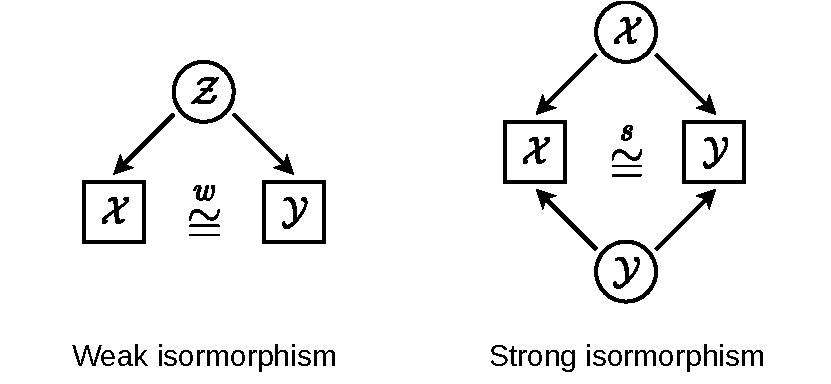
\includegraphics[width=0.6\textwidth,keepaspectratio]{Chapitre1/figures/isomorphism.pdf}
%   \caption{Semi-strong and weak isomorphisms. The direction of the arrow indicates that one network
%   is a mass splitting of the other.}
%   \label{fig:strong_weak}
% \end{figure}
Similar to the Wasserstein distance, a Monge version of the GW distance,
known as \textit{Gromov-Monge} (GM) distance, is defined as
\begin{equation}
  \text{GM}(\cX, \cY) =
  \inf_{\varphi \in \cT(\mu_X, \mu_Y)} || c_X - \varphi^* c_Y ||_{L^p(X^2, \mu_X \otimes \mu_X)},
\end{equation}
where, recall that $\cT(\mu, \nu)$ is the set of transport maps from $\mu$ to $\nu$.
The GM distance suffers the same limitations as the Monge's problem,
notably the existence of the transport map and the asymmetry of the metric.
It is easy to see that $\cZ$ is a mass splitting of $\cX$ if and only if $\text{GM}(\cZ, \cX) = 0$.
The equality between GM and GW distances has also attracted much interest
in the mathematics community, see \citep{Memoli22} for a comprehensive and up-to-date review.

The following result is very handy as it allows us to flexibly switch between the GW and GM distances.
%%%%%%%%%%%%%%%%%%%%%%%%%%%%%%%%%%%%%%%%%%%%%%%%
\begin{corollary}[Theorem 14 in \citep{Memoli21}]
  \label{GW_mGW}
  Let $\cX$ and $\cY$ be two measure networks, then
  \begin{equation*}
    \text{GW}(\cX, \cY) = \inf_{\cZ \in \ms(\cX)} \text{GM}(\cZ, \cY)
    = \inf_{\cZ \in \ms(\cY)} \text{GM}(\cZ, \cX).
  \end{equation*}
  Moreover, the infima are always attained: there exist two measure networks $\cZ_x \in \ms(\cX)$ and
  $\cZ_y \in \ms(\cY)$ such that
  $\text{GW}(\cX, \cY) = \text{GM}(\cZ_x, \cY) = \text{GM}(\cZ_y, \cX)$.
\end{corollary}
%%%%%%%%%%%%%%%%%%%%%%%%%%%%%%%%%%%%%%%%%%%%%%%%
\begin{proposition}[Relations of GW and GM with isomorphism] \label{prop:GW_iso}
  Let $\cX$ and $\cY$ be two measure networks.
  \begin{enumerate}
    \item $\cX$ and $\cY$ are weakly isomorphic if and only if $\text{GW}(\cX, \cY) = 0$.
    \item $\cX$ and $\cY$ are semi-strongly isomorphic if and only if
    $\text{GM}(\cX, \cY) = \text{GM}(\cY, \cX) = 0$.
  \end{enumerate}
\end{proposition}
%%%%%%%%%%%%%%%%%%%%%%%%%%%%%%%%%%%%%%%%%%%%%%%%
%%%%%%%%%%%%%%%%%%%%%%%%%%%%%%%%%%%%%%%%%%%%%%%%
\begin{proof}
  If $\cX$ and $\cY$ are weakly isormorphic, then there exists a common mass splitting $\cZ$ of $\cX$ and $\cY$,
which means $\text{GM}(\cZ, \cY) = 0$. By \cref{GW_mGW},
$\text{GW}(\cX, \cY) = \text{GM}(\cZ, \cY) = 0$. Conversely, if $\text{GW}(\cX, \cY) = 0$,
then by \cref{GW_mGW}, there exists $\cZ \in \ms(\cX)$ such that $\text{GM}(\cZ, \cY) = 0$.
But this means $\cZ \in \ms(\cY)$. We conclude that $\cX$ and $\cY$ are weakly isormorphic
since $\cZ$ is the common mass splitting. The equivalence between semi-strong isormorphism and
GM follows immediately from the definition.
\end{proof}
\Cref{prop:GW_iso} allows us to characterize the equivalence classes of GW distance in the
setting of networks. In particular,
\begin{proposition}
  [Theorems 2.3 and 2.4 in \citep{Chowdhury19}]
  GW distance defines a metric on the space of networks, up to weak isomorphism.
\end{proposition}
%%%%%%%%%%%%%%%%%%%%%%%%%%%%%%%%%%%%%%%%%%%%%%%%
\begin{corollary}[Relation between weak isomorphism and mass splitting]
  \text{ }
\begin{enumerate}
  \item If $\cZ$ is a mass splitting of $\cX$, then $\cX$ and $\cZ$ are weakly isomorphic
  (since $\cZ$ is the common mass splitting).
  \item If two networks are weakly isomorphic, then so are their mass splittings.
\end{enumerate}
\end{corollary}
\begin{proof}
  If $\cZ$ is a mass splitting of $\cX$, then $\cZ$ is the common mass splitting.
  So, $\cX$ and $\cZ$ are weakly isomorphic.

  If $\cX$ and $\cY$ are weakly isomorphic, then they have a common mass splitting $\cZ$.
  By \Cref{prop:GW_iso}, we have $\gw(\cX, \cZ) = \gw(\cY, \cZ) = 0$.
  Now, suppose $\cX' \in \ms(\cX)$ and $\cY' \in \ms(\cY)$, then
  $\gw(\cX, \cX') = \gw(\cY, \cY') = 0$. By triangle inequality, we deduce that
  $\gw(\cX', \cZ) = \gw(\cY', \cZ) = 0$. So, $\cZ$ is the common mass splitting
  of $\cX'$ and $\cY'$, meaning that they are weakly isomorphic.
\end{proof}

%%%%%%%%%%%%%%%%%%%%%%%%%%%%%%%%%%%%%%%%%%%%%%%%
\subsection{Optimization and algorithm}
%%%%%%%%%%%%%%%%%%%%%%%%%%%%%%%%%%%%%%%%%%%%%%%%
For $n \in \bbN^*$, we define the probability simplex by
$\Sigma_n := \{ p \in \bbR^n_{> 0}: \sum_i p_i = 1 \}$.
In discrete setting, given two matrices (not necessarily symmetric)
$C^x \in \bbR^{m \times m}, C^y \in \bbR^{n \times n}$ and histograms
$\mu_X \in \Sigma_m, \mu_Y \in \Sigma_n$, the GW problem reads
\begin{align}
  \label{eq:discrete_gw}
  \min_{P \in U(\mu, \nu)} \sum_{i,j,k,l} |C^x_{ik} - C^y_{jl}|^p \; P_{ij} P_{kl}
\end{align}
For convenience, we write
$\sum_{i,j,k,l} |C^x_{ik} - C^y_{jl}|^p \; P_{ij} P_{kl} = \langle C \otimes P, P \rangle$,
where the $4$D-tensor cost $C = |C^x - C^y|^p$ is defined by $C_{ijkl} = (C^x_{ik} - C^y_{jl})^p$.
Intuitively, the Wasserstein distance to linear assignment problem is
the same as the GW distance to quadratic assignment problem (QAP) \citep{Koopmans57},
where the permutation matrix is replaced by a doubly stochastic one.
While the QAP is known to be NP-hard, introducing more flexibility to the alignment matrix
does not necessarily ease the optimization. Furthermore,
the computational complexity of the $4$D-tensor cost is prohibitive in most applications.
For these reasons, the current approach to solve the discrete GW usually consists of
an efficient approximation technique and additional structures on the cost tensor.
In this section, we discuss both components in more details.

\subsubsection{Structure of the cost tensor}
To handle the cost tensor, an efficient, yet easy to implement strategy is to make it
as decomposable as possible. Given its form $C = |C^x - C^y|^p$, the decomposability
can be achieved by choosing $p=2$. To see this, let us recall the following results.
\begin{lemma}[Generalization of Proposition 1 in \citep{Peyre16}]
  \label{lemma_peyre16}
Denote $\oplus$ the Kronecker sum.
For any matrix $M$, we write $M^{\odot 2} := M \odot M$, where $\odot$
is the element-wise multiplication. Given $A \in \bbR^{n_1 \times d_1},
B \in \bbR^{n_2 \times d_2}$ and $P \in \bbR^{d_1 \times d_2}$, we define
$\vert A - B \vert^2 \otimes P \in \bbR^{n_1 \times n_2}$ by
$(\vert A - B \vert^2 \otimes P)_{ij} = \sum_{k,l } |A_{ik} - B_{jl}|^2 P_{kl}$.
Then, $\vert A - B \vert^2 \otimes P = A^{\odot 2} P_{\# 1} \oplus B^{\odot 2} P_{\# 2} - 2 A P B^T$.
\end{lemma}
In particular, in the case of GW distance, for any $P \in U(\mu_X, \mu_Y)$, we have
\begin{align}
  \label{eq:cost_tensor_full}
  \langle |C^x - C^y|^2 \otimes P, P \rangle
  = \langle (C^x)^{\odot 2} \mu_X, \mu_X \rangle + \langle (C^y)^{\odot 2} \mu_Y, \mu_Y \rangle
  - 2 \langle C^x P (C^y)^T, P \rangle,
\end{align}
where $\langle (C^x)^{\odot 2} \mu_X, \mu_X \rangle + \langle (C^y)^{\odot 2} \mu_Y, \mu_Y \rangle$
is a constant independent of $P$ and has computational cost of $O(m^2 + n^2)$.
The cost of $C^x P (C^y)^T$ is $O(m^2 n + n^2m)$.
So, the overall computational complexity is reduced from $O(m^2 n^2)$ to $O(m^2 n + n^2 m)$.
Moreover, if the input matrices $C^x, C^y$ are factorizable,
then this cost can be even further reduced, for both constant term and $C^x P (C^y)^T$.
For example, the squared distance matrix is factorizable,
thanks to two lemmas below in \citep{Meyer21b}.
\begin{lemma}[Exact low-rank factorization of squared distance matrix]
  If $A = (a_1,...,a_m) \in \bbR^{m \times d}$ and $B = (b_1,...,b_n) \in \bbR^{n \times d}$,
then the matrix $D \in \bbR^{m \times n}$ defined by
$D_{ij} = \vert\vert a_i - b_j \vert\vert_2^2$ can be decomposed as $D = D_a D_b^T$, where
$D_a = (A^{\odot 2} 1_d, 1_m, -\sqrt{2} A) \in \bbR^{m \times (d+2)}$ and
$D_b = (1_n, B^{\odot 2} 1_d, \sqrt{2} B) \in \bbR^{n \times (d+2)}$.
\end{lemma}
\begin{lemma}[Element-wise square trick for factorizable matrix]
  For $x \in \bbR^d$, define $\varphi(x) = \text{vec}(xx^T) \in \bbR^{d^2}$.
  Suppose $A = B C^T$, where $B \in \bbR^{m \times d}$ and $C \in \bbR^{n \times d}$.
  By writing $B$ as $[b_1, ..., b_m]^T$ and $C$ as $[c_1, ..., c_n]^T$, define
  $\widetilde{B} = [\varphi(b_1), ..., \varphi(b_m)]^T \in \bbR^{m \times d^2}$ and
  $\widetilde{C} = [\varphi(c_1), ..., \varphi(c_n)]^T \in \bbR^{n \times d^2}$.
  Then $A^{\odot 2} = \widetilde{B} \widetilde{C}^T$. In particular, $A^{\odot 2}$ is also
  factorizable and has rank $d^2$. In PyTorch, $\widetilde{B}$ can be calculated by:
  \texttt{torch.einsum("ij,ik->ijk", B, B).reshape(B.shape[0], B.shape[1]**2)}.
\end{lemma}
We deduce that, if $C^x = D_x D_x^T, (C^x)^{\odot 2} = \widetilde{D}_x \widetilde{D}_x^T$
and $C^y = D_y D_y^T, (C^y)^{\odot 2} = \widetilde{D}_y \widetilde{D}_y^T$,
with $D_x \in \bbR^{m \times d_x}, \widetilde{D}_x \in \bbR^{m \times d_x^2},
D_y \in \bbR^{n \times d_y}$ and $\widetilde{D}_y \in \bbR^{n \times d_y^2}$ are low-rank matrices
with $d_x \ll m$ and $d_y \ll n$, we have
\begin{align}
  \langle \vert C^x - C^y \vert^2 \otimes P, P \rangle
  &= (C^x)^{\odot 2} P_{\# 1} \oplus (C^y)^{\odot 2} P_{\# 2} - 2 C^x P (C^y)^T \\
  &= \mu_X^T \widetilde{D}_x \widetilde{D}_x^T \mu_X
  + \mu_Y^T \widetilde{D}_y \widetilde{D}_y^T \mu_Y - 2 \langle D_x D_x^T P D_y D_y^T, P \rangle
\end{align}
Comparing to \Cref{eq:cost_tensor_full}, the computational costs are now much cheaper,
where for the constant term, it is $O(m d_x^2 + n d_y^2)$, and for $C^x P (C^y)^T$,
it is $O(mn(d_x + d_y) + (m+n) d_x d_y)$. If the distance matrix is not factorizable,
one can consider the low-rank approximation,
whose implementation details can be found in \citep{Meyer21a}.

We also stress that, exploiting the decomposability is not the only way to reduce the computational
complexity. For an overview of more complicated strategies,
interested readers may consult Table 1 in \citep{Li23} and the reference therein.

\subsubsection{Approximation technique}
The common principle behind many current methods for solving the GW problem
is the linearization of the objective function,
so that each iteration boils down to solving a (possibly regularized)
OT problem. However, given the nonconvex nature of the GW problem, they also share
a common limitation, where only local, but not global convergence is guaranteed.
In what follows, we briefly discuss several solvers using this principle.
We note that, however, in some particular situations, it is possible to achieve the
global convergence. For example, when $p=2$ and $C^x, C^y$ are squared Euclidean distance,
\citep{Ryner23} propose to apply the cutting-plane method to a tractable relaxation of the GW problem
and show that this algorithm converges to the global optimum.

\paragraph{1. Condition gradient descent} \citep{Vayer19b} directly estimate the GW problem by using
the Frank-Wolfe algorithm, also known as \textit{condition gradient descent}
\citep{Frank56,Jaggi13}. More precisely, each iteration requires
solving an unregularized OT problem, whose cost $C \otimes P^{(t)}$ is the gradient
involving the previous OT plan, then interpolating betweeen the newly acquired OT plan and
the previous one using a certain line search strategy. Since the objective function is nonconvex,
the Frank-Wolfe algorithm only guarantee the convergence to a local stationary point \citep{Julien16}.

\paragraph{2. Projected gradient descent} Similar to the Wasserstein distance,
one can also approximate the GW distance with entropic regularization.
\begin{align}
  \min_{\substack{P \in U(\mu_X, \mu_Y)}} \langle C \otimes P, P \rangle + \varepsilon \kl(P | \gamma),
\end{align}
for some relevant reference histogram $\gamma \in \bbR^{m \times n}_{> 0}$ and $4$D-tensor cost $C$.
For example, $\gamma = 1_{m \times n}$ corresponds to using the negative entropy as regularizer.
To solve this problem, \citep{Peyre16,Solomon16} propose to use projected gradient descent,
where each iteration boils down to solving an entropic OT problem. More precisely,
\begin{lemma}
  [Generalization of Proposition 2 in \citep{Peyre16}] Given a matrix $M \in \bbR^{m \times n}$,
  consider the (entropic fused GW) problem
  \begin{align}
    \label{eq:fused_egw}
    \min_{\substack{P \in U(\mu_X, \mu_Y)}} \langle C \otimes P, P \rangle
    + \langle M, P \rangle + \varepsilon \kl(P | \gamma),
  \end{align}
  Then the PGD iteration reads: for any learning rate $\eta > 0$,
  \begin{align}
    P^{(t+1)} = \argmin_{P \in U(\mu_X, \mu_Y)}
    \eta \langle C \otimes P^{(t)} + M, P \rangle
    + \varepsilon \kl \left( P \big| \gamma^{\eta} \odot (P^{(t)})^{1 - \eta} \right).
  \end{align}
\end{lemma}
% \begin{proof}
%   Denote $F(P) = \langle C \otimes P, P \rangle + \langle M, P \rangle + \varepsilon \kl(P | \gamma)$.
%   Then $\nabla F(P) = C \otimes P + M + \varepsilon \log \frac{P}{\gamma}$.
%   The PGD iterate reads: for $\tau > 0$,
%   \begin{align}
%     P^{(t+1)} = \text{proj}^{\kl}_{U(\mu_x, \mu_y)}
%     \left( P^{(t)} \odot e^{-\tau \nabla F(P^{(t)})} \right)
%   \end{align}
%   Recall that $\text{proj}^{\kl}_{U(\mu_x, \mu_y)}(K) =
%   \argmin_{P \in U(\mu_x, \mu_y)} - \varepsilon \langle \log K, P \rangle + \varepsilon H(P)$.
%   Denote $\eta = \tau \varepsilon$. We have
%   \begin{align}
%     \log K &= \log \left( P^{(t)} \odot e^{-\tau \nabla F(P^{(t)})} \right) =
%     \log P^{(t)} - \tau (C \otimes P^{(t)} + M)  - \tau \varepsilon \log \frac{P^{(t)}}{\gamma} \\
%     &= - \tau (C \otimes P^{(t)} + M) + \log \left( \gamma^{\eta} \odot (P^{(t)})^{1 - \eta} \right)
%   \end{align}
%   So,
%   \begin{align}
%     &- \varepsilon \langle \log K, P \rangle + \varepsilon H(P) \\
%     &= \eta \langle C \otimes P^{(t)} + M, P \rangle
%     - \varepsilon \langle P, \log \left( \gamma^{\eta} \odot (P^{(t)})^{1 - \eta} \right) \rangle
%     + \varepsilon H(P) \\
%     &= \eta \langle C \otimes P^{(t)} + M, P \rangle +
%     \varepsilon \kl \left( P \big | \gamma^{\eta} \odot (P^{(t)})^{1 - \eta} \right)
%     - m \left( \gamma^{\eta} \odot (P^{(t)})^{1 - \eta} \right),
%   \end{align}
%   where $m(Q) = \sum_{i,j} Q_{ij}$ is the mass of measure $Q$. The result then follows.
% \end{proof}
As observed in \citep{Peyre19}, $\eta = 1$ usually works well in practice,
where the sequence $(P^{(t)})_t$ converges empirically. However, the convergence analysis remains
unexplored. As a side note, adding regularization to the GW distance also incurs bias,
similar to the entropic OT. Inspired by the Sinkhorn divergence,
\citep{Bunne19} apply the same strategy to debiase the entropic GW,
but there is no theoritical guarantee with their approach.

\paragraph{3. (Inexact) Bregman proximal point} Inspired by IPOT \citep{Xie20}, \citep{Xu19, Xu19b}
propose to use the Bregman proximal point (BPP) method, where at each iteration, we solve
\begin{align}
  \min_{P \in U(\mu_X, \mu_Y)} \langle C \otimes P, P \rangle + \eta \; \kl(P | P^{(t)})
\end{align}
This is nothing but the entropic GW problem presented in the second approach, thus can be solved
with the PGD algorithm. The resulting sequence only guarantees that
every limit point is a stationary point \citep{Xu19}.

\paragraph{4. Block coordinate descent} Apart from using entropic regularization,
one can also consider the following problem
\begin{align}
  \label{eq:coot}
  \min_{\substack{P, Q \in U(\mu_X, \mu_Y)}} \langle C \otimes P, Q \rangle.
\end{align}
Clearly, this is a lower bound of the GW distance since we no longer require two couplings to be equal.
The bound can become the equality, for example, when $p=2$ and $C^x, C^y$ are the Euclidean distances.
This means that dropping the equality constraint does not change the minimum nor the minimizer.
More discussion on such situations can be found in \Cref{subsec:GWLB}.
In these cases, we can apply the block coordinate descent (BCD) algorithm,
where in each iteration, we alternatively fix one coupling and solve the OT problem
with respect to the other. Since the objective function is smooth,
this algorithm can only guarantee the convergence to a stationary point \citep{Tseng01}.
This lower-bound strategy can also be easily extended to the general problem \ref{eq:fused_egw},
where it is enough to rewrite the objective function as
\begin{align}
  \min_{\substack{P, Q \in U(\mu_X, \mu_Y)}} \langle C \otimes P, Q \rangle
  + \langle \frac{M}{2}, P + Q \rangle + \frac{\varepsilon}{2} \kl(P | \gamma)
  + \frac{\varepsilon}{2} \kl(Q | \gamma),
\end{align}
with $P = Q$. Moreover, one can ignore the equality constraint without impacting the minimum,
under exactly the same conditions as in Problem \ref{eq:coot}.

\paragraph{5. Bregman alternating projected gradient}
Another way to use the lower bound is in \citep{Li22}.
\begin{align}
  \min_{\substack{(P, Q) \in \cC_1 \times \cC_2 \\ P = Q}} \langle C \otimes P, Q \rangle
\end{align}
where $\cC_1 = \{ P \geq 0: P_{\# 1} = \mu_X \}$ and $\cC_2 = \{ Q \geq 0: Q_{\# 2} = \mu_Y \}$,
They propose to use the Bregman alternating projected gradient (BAPG), whose iterates read:
for a given learning rate $\eta > 0$,
\begin{enumerate}
  \item $P^{(t+1)} = \argmin_{P \in \cC_1} \langle C \otimes Q^{(t)}, P \rangle + \eta \kl(P | Q^{(t)})$.
  \item $Q^{(t+1)} = \argmin_{Q \in \cC_2} \langle C \otimes P^{(t+1)}, Q \rangle + \eta \kl(Q | P^{(t+1)})$.
\end{enumerate}
However, BAPG has two main drawbacks: it only converges asymptotically to a critical point and
the iterates do not necessarily satisfy the marginal constraints. To overcome these issues,
the authors propose the hybrid Bregman Projected Gradient (hBPG),
which consists of initializing with the solution of the entropic GW problem,
then applying the BPP method discuss previously. Local linear convergence result
is also established for hBPG.

\paragraph{6. Saddle point approximation} Similar to \citep{Koehl19},
\citep{Koehl23} use the framework from statistical physics and approximate the GW distance by
the limit of a decreasing sequence of free energies. Rougly speaking, at each iteration,
this boils down to iteratively estimating the free energy by using the saddle point approximation.
Formally, we fix a decreasing sequence of temperatures $(\beta_t)_t$ converging to $0^+$.
At the iteration $t$, set $Q^{(0)} = P^{(t-1)}$. Then, for $k \geq 1$,
run the following iterative scheme until convergence.
\begin{enumerate}
  \item Calculate the new OT cost $C^{(k)} = C \otimes Q^{(k)}$.
  \item Solve the non-linear system of equations for $u \in \bbR^m$ and $v \in \bbR^n$.
  \begin{align*}
    \begin{cases}
      \sum\limits_{j=1}^n \varphi \big( \beta_t (u + v_j + C^{(k)}_{\cdot, j}) \big) = \mu_X \\
      \sum\limits_{i=1}^m \varphi \big( \beta_t (u_i + v + C^{(k)}_{i, \cdot}) \big) = \mu_Y
    \end{cases}
  \end{align*}
  \item Compute $Q^{(k+1)} = \varphi \big( \beta_t (u \oplus v + C^{(k)}) \big)$.
\end{enumerate}
Finally, set $P^{(t)} = Q^{(k)}$ and repeat the procedure.
Here $\varphi(x) = \frac{e^{-x}}{e^{-x} - 1} + \frac{1}{x}$, for $x \neq 0$ and $\varphi(0) = 1/2$.
In theory, while the GW distance is known to be the limit of the free energy when
the temperature tends to $0$, the convergence analysis of this algorithm remains unexplored.

%%%%%%%%%%%%%%%%%%%%%%%%%%%%%%%%%%%%%%%%%%%%%%%%
\subsection{Beyond GW distance}
%%%%%%%%%%%%%%%%%%%%%%%%%%%%%%%%%%%%%%%%%%%%%%%%

\paragraph{Fused GW distance} Structured data - an object made of two components:
structure and feature information, is ubiquitous in practical situations.
Typical examples include attributed graph, whose node is assigned with a label, or
cortical surface whose vertice is associated to a vectorial representation of the
functional activation map, or in supervised learning, the dataset is a set of example-label pairs.
By construction, neither GW nor Wasserstein distance is designed to handle this kind of data.
\citep{Vayer19b} propose a simple, yet efficient method called
\textit{Fused GW} (FGW) distance, which is able to take into account both types of information.
It is convenient to cast structured data as an attributed graph $\cX = (C^x, F^x, \mu_X)$,
where $C^x$ is the similarity matrix, $F^x$ is the set of features associated to the nodes and
$\mu_X$ is the histogram assigned to the nodes. Given two attributed graphs
$\cX = (C^x, F^x, \mu_X)$ and $\cY = (C^y, F^y, \mu_Y)$, for $\alpha \in [0, 1]$, we define
\begin{align}
  \text{FGW}_{\alpha}(\cX, \cY) = \inf_{P \in U(\mu_X, \mu_Y)}
  (1 - \alpha) \langle C \otimes P, P \rangle + \alpha \langle M, P \rangle,
\end{align}
where the $4$D-tensor cost $C$ is usually of the form $C = |C^x - C^y|^p$ as in the GW distance,
The matrix $M$ usually represents the pairwise similarity amongst features, typically
$M_{ij} = || a_i - b_j||^p$, where $a_i \in F^x$ and $b_j \in F^y$. Note that,
the presence of feature information indicates that the measure-preserving isometries
for structure information needs to be also feature-preserving.
The structure of the objective function allows FGW to interpolate
between the OT and GW distances, depending on the asymptotic behavior of $\alpha$ \citep{Vayer19b}.

Any solver for GW can be easily applied to the FGW. Instead of using predefined feature,
it is also possible to learn it simultaneously with the alignment matrix,
for example in \citep{Xu19}. It can also be easily integrated into many OT-based divergences,
for example low-rank GW \citep{Meyer21b},
Keypoint-guided OT \citep{Gu22}, Information-maximizing OT \citep{Chuang23},
fused unbalanced GW \citep{Thual22}.
In supervised learning, the main idea of FGW is also shared in other OT-based divergences,
for example the OT Dataset distance between datasets \citep{Melis20},
Joint-distribution OT \citep{Courty17}, or Transportation $L^p$ distance \citep{Thorpe17}.

\paragraph{Marginal relaxation in GW distance} Inspired by the recent interest and development
on UOT \citep{Liero18}, the GH-based distances between mm-spaces can be extended to
the unbalanced setting. More precisely, given two mm-spaces
$\cX = (X, d_X, \mu_X)$ and $\cY = (Y, d_Y, \mu_Y)$, \citep{Ponti20}
study the unbalanced extension of the $L_p$-transportation distance called
\textit{Sturm-Entropic-Transport distance}, defined as
\begin{equation}
  \text{D}_{\text{ET}}(\cX, \cY) =
  \inf_{Z, f, g} UW_{Z, p}\big( (f(X), f_{\#} \mu_X), (g(Y), g_{\#} \mu_Y) \big),
\end{equation}
where the infimum is taken over all complete and separable metric spaces $Z$ and
isometric embeddings $f: X \to Z$ and $g: Y \to Z$. \citep{Sejourne20} introduce the
unbalanced GW (UGW) divergence: given two relaxation parameters
$\rho_1, \rho_2 > 0$ and two Csizar divergences $D_{\varphi_1}, D_{\varphi_2}$, they define
\begin{equation}
  \text{UGW}_{\lambda}(\cX, \cY) =
  \inf_{ \pi \in U(\mu_X, \mu_Y)} \int |d_X - d_Y|^p d\pi d\pi +
  \rho_1 D_{\varphi_1}^{\otimes 2}(\pi_{\# 1} | \mu_X) +
  \rho_2 D_{\varphi_2}^{\otimes 2}(\pi_{\# 2} | \mu_Y).
\end{equation}
Here, $D_{\varphi}^{\otimes 2}$ denotes the \textit{quadratic divergence}
$D_{\varphi}^{\otimes 2}(\mu | \nu) := D_{\varphi}(\mu \otimes \mu | \nu \otimes \nu)$.
This structure of product measures is particularly useful in the study of theoretical
and practical properties of UGW, namely the existence of solution,
the relation with conic formulation \citep{Sejourne20} and the robustness to outliers \citep{Tran23}.

\citep{Zhang21} propose the unbalanced bidirectional Gromov-Monge divergence defined as:
for $\lambda_x, \lambda_y > 0$,
\begin{equation}
  \begin{split}
    \text{UBGM}_{\lambda}(\cX, \cY) = \inf_{\substack{f: X \to Y \\ g: Y \to X}}
  \Delta_p(f,g, X, Y) + \lambda_x \text{D}_{\varphi_x}(g_{\#} \mu_Y | \mu_X)
  + \lambda_y \text{D}_{\varphi_y}(f_{\#}\mu_X | \mu_Y).
  \end{split}
\end{equation}
where $D_{\varphi_x}$ and $D_{\varphi_y}$ are divergences on $\mathcal M^+_1(X)$ and $\mathcal M^+_1(Y)$,
respectively. Here, the authors define a divergence $D$ on $\mathcal M^+_1(Z)$ as a function
$D: \mathcal M^+_1(Z) \times \mathcal M^+_1(Z) \to \bbR_{\geq 0}$ such that
$D(P | Q) = 0$ if and only if $P = Q$. In particular, when $\mu_X$ and $\mu_Y$
are probability measures and $D_{\varphi_x}, D_{\varphi_y}$ are maximum mean discrepancies,
the convergence rate of the empirical measures can be computed.

Other unbalanced extensions of the GW distance include the semi-relaxed GW divergence \citep{Vincent22},
where only one marginal is relaxed, or the partial GW \citep{Chapel20}
motivated by the partial OT \citep{Caffarelli10, Figalli10}, where the mass of the transport plan
is bounded above. We note that both divergences can be obtained from UGW,
by choosing appropriate relaxation parameters and divergences.
Another alternative is the outlier-robust GW (RGW) \citep{Kong23}. It combines GW distance with
the marginal relaxation of UOT from \citep{Liero18} and
the KL relaxations as constraints from \citep{Balaji20},
though the authors do not give proper credits to these prior works.
Similar to UGW, RGW also enjoys provable robustness property and shows strong performance
in various graph learning tasks, where outliers present.

%%%%%%%%%%%%%%%%%%%%%%%%%%%%%%%%%%%%%%%%%%%%%%
\section{Inexact Bregman Proximal Point method for entropic unbalanced OT}
\label{sec:input}

This section is an ongoing work on an alternative solver for the entropic UOT problem
\ref{eq:discrete_ent_uot}, which has not yet been studied in the literature,
to the best of our knowledge.
We called this approach \textit{INexact Proximal Unbalanced optimal Transport} (INPUT),
since it is a straightforward application of the inexact Bregman Proximal Point (BPP) algorithm
to the UOT problem. We present the derivation of INPUT, then illustrate how
it can overcome the limitations of the MM and Sinkhorn-based methods,
while being orders of magnitude faster in our toy experiments. Despite the simplicity,
its convergence analysis remains a challenging open problem and is under our active research.

\subsection{Motivation, optimization and algorithm}

While the Bregman Proximal Point method \citep{Chen93} applies to the class of Bregman divergences,
we will exclusively focus on the KL divergence throughout this thesis.
\begin{definition}
  Given a nonepmpty closed convex set of $E \subset \bbR^d_{\geq 0}$
  and a proper closed convex function $f: E \to \bbR$, consider the following
  convex optimization problem
  \begin{equation*}
    \min_{x \in E} f(x)
  \end{equation*}
  For learning rate $\eta > 0$, the exact BPP scheme with respect to the KL divergence reads
  \begin{equation}
    \label{eq:bppa}
    x^{(t+1)} = \argmin_{x \in E} f(x) + \eta \kl(x, x^{(t)}),
  \end{equation}
  and the inexact BPP scheme reads
  \begin{equation}
    \label{eq:bppa_inexact}
    x^{(t+1)} \approx \argmin_{x \in E} f(x) + \eta \kl(x, x^{(t)}).
  \end{equation}
  Here, $x^{(t+1)}$ is only an approximate solution in some sense.
\end{definition}
When applying to Problem \ref{eq:discrete_ent_uot}, the exact BPP iteration boils down to solving
\begin{align}
  \label{eq:bpp_uot}
  P^{(t+1)} &= \argmin_{P \in \bbR^{m \times n}_{\geq 0}}
  \langle C, P \rangle + \rho_1 \kl(P_{\# 1} | \mu)
  + \rho_2 \kl(P_{\# 2} | \nu) + \varepsilon \kl(P | \gamma) + \eta \kl(P | P^{(t)}) \\
  &= \argmin_{P \in \bbR^{m \times n}_{\geq 0}}
  \left \langle C - \eta \log \frac{P^{(t)}}{\gamma}, P \right \rangle
  + \rho_1 \kl(P_{\# 1} | \mu) + \rho_2 \kl(P_{\# 2} | \nu) + (\varepsilon + \eta) \kl(P | \gamma)
\end{align}
This is nothing but an entropic UOT problem with modified cost and regularization.
Thus, any solvers discussed in \Cref{sub:uot_optim} can be used. In particular,
by construction, BPP is naturally applicable to the unregularized UOT.
In practice, the exact BPP may not be an efficient algorithm to solve the UOT problem since
it requires solving \textbf{exactly} many entropic subproblems. This can be computationally expensive,
especially when the learning rate is small.
While the inexact method has recently been applied to the balanced OT \citep{Xie20,Yang22},
we are not aware of any extension to the unbalanced counterpart.
Our proposed method follows directly from \citep{Xie20}, which is simple to implement and
usually performs well in practice. In particular,
we only require running a few Sinkhorn iterations for each entropic subproblem and
use the approximated coupling as input for the next BPP iteration.
The algorithmic details of INPUT can be found in \Cref{alg:isppa}.
\begin{algorithm}[t]
  \caption{INPUT algorithm for Problem \ref{eq:discrete_ent_uot}.}
  \label{alg:isppa}
\begin{algorithmic}[1]
  \STATE \textbf{Input:} cost matrix $C \in \bbR^{m \times n}$,
  measures $\mu \in \bbR^m_{> 0}, \nu \in \bbR^n_{> 0}, \gamma \in \bbR^{m \times n}_{> 0}$,
  regularization $\varepsilon \geq 0$, relaxation parameters $\rho_1, \rho_2 > 0$,
  learning rate $\eta > 0$.
  \FOR{$t=1, \dots, T$}
  \STATE Calculate new cost: $C^{(t+1)} \gets C - \eta \log \Big( \frac{P^{(t)}}{\gamma} \Big)$.
  \STATE Solve approximatively the entropic UOT problem
  \begin{align*}
    P^{(t+1)} \approx \argmin_{P \geq 0} \; \langle C^{(t+1)}, P \rangle +
    \rho_1 \kl(P_{\# 1} | \mu) + \rho_2 \kl(P_{\# 2} | \nu) + (\varepsilon + \eta) \kl(P | \gamma).
  \end{align*}
  \ENDFOR
  \STATE \textbf{Output:} transport plan $P^{(T)}$.
\end{algorithmic}
\end{algorithm}

\subsection{Convergence analysis in the exact setting}

Let us start with the convergence analysis in case of BPP iteration \ref{eq:bpp_uot}.
Thanks to Lemma 3.3 and Theorem 3.4 in \citep{Chen93}, if $P^*$ is a minimizer of
Problem \ref{eq:discrete_ent_uot}, then
\begin{enumerate}
  \item The sequence $\big( \kl(P^*, P^{(t)}) \big)_t$ is nonincreasing and converges to $0$.
  \item The sequence $\big( F(P^{(t)}) \big)_t$ is nonincreasing and
  \begin{align}
    \label{eq:chen_teboulle}
    F(P^{(t)}) - F(P^*) \leq \frac{\eta}{t} \kl(P^* | P^{(0)}).
  \end{align}
\end{enumerate}
The upper bound \ref{eq:chen_teboulle} can be improved by further exploiting the property of
the objective function of Problem \ref{eq:discrete_ent_uot}.
First, we introduce the notions of relative smoothness \citep{Bauschke17} and
strong convexity \citep{Lu18} of a function with respect to the KL divergence.
\begin{definition}
  \label{def:smooth-convex}
  Let $f:C \to \bbR$ be a differentiable convex function.
  Given $L \geq 0$, we say that $f$ is $L-$smooth relative to the KL divergence
  if for any $x, y \in C$,
  \begin{equation*}
    f(x) \leq f(y) + \langle \nabla f(y), x - y \rangle + L \; \kl(x, y).
  \end{equation*}
  Given $l \geq 0$, we say $f$ is $l-$strongly convex relative to the KL divergence
  if for any $x, y \in C$,
  \begin{equation*}
    f(x) \geq f(y) + \langle \nabla f(y), x - y \rangle + l\; \kl(x, y).
  \end{equation*}
\end{definition}

\begin{lemma}
  \label{lemma:convex-smoothness}
  $F$ is $\varepsilon$-strongly convex and $(\lambda_1 + \lambda_2 + \varepsilon)$-relatively smooth
  with respect to the KL divergence.
\end{lemma}
The following result is a simple generalization of Theorem 3.1 in \citep{Lu18}.
\begin{proposition}[Convergence rate of exact BPP for Problem \ref{eq:discrete_ent_uot}]
  \label{prop:convergence-exact-sppa}
  For every $\eta > 0$, exact BPP decreases the value of $F(\cdot)$ with each iteration $t$:
  the sequence $\big( F(\pi^{(t)}) \big)_t$ is monotonically decreasing.
  Moreover, if $\varepsilon \leq \eta \leq \lambda_1 + \lambda_2 + \varepsilon$,
  then we have
  \begin{align*}
    F(\pi^{(t)}) - F(\pi^*)
    \leq \frac{\varepsilon}{\left( 1 +
    \frac{\varepsilon (\lambda_1 + \lambda_2 + \varepsilon)}{\eta (\lambda_1 + \lambda_2)} \right)^t - 1}
    \kl(\pi^* | \pi^{(0)}).
  \end{align*}
\end{proposition}
It is not difficult to check that this bound is weaker than the one in
Inequality (\ref{eq:chen_teboulle}). Indeed,
\begin{align*}
  \frac{\varepsilon}{\left( 1 +
  \frac{\varepsilon (\lambda_1 + \lambda_2 + \varepsilon)}{\eta (\lambda_1 + \lambda_2)} \right)^t - 1}
  \leq \frac{\varepsilon}{\frac{t \varepsilon(\lambda_1 + \lambda_2 + \varepsilon)}{\eta (\lambda_1 + \lambda_2)}}
  = \frac{\eta}{t} \frac{\lambda_1 + \lambda_2}{\lambda_1 + \lambda_2 + \varepsilon}
  \leq \frac{\eta}{t}.
\end{align*}

\subsection{Convergence analysis in the inexact setting}

Despite the simplicity, it is difficult to analyze the convergence of INPUT.
In particular, while it is an immediate extension of the work of \citep{Xie20} on the balanced OT,
their proof techniques of the convergence can not be adapted to the unbalanced setting.
This is because they rely on the property of the set of admissible couplings,
which is not available in the UOT. Moreover, the assumptions and conditions are also
not trivial to verify in practice, thus their convergence results are mostly of theoretical interest.

The convergence analysis of the inexact BPP has already been studied at the same time
as the exact one. Typically, one can control the approximation error using
$\varepsilon$-subdifferential \citep{Burachik97,Kiwiel97},
or bounded subgradient \citep{Eckstein98,Rockafellar76}, to name a few.
We are studying the literature in this domain to identify the relevant criteria, which are
amenable to study the convergence and to verify in practice.

\subsection{Illustration on toy example}

\paragraph{Experimental setup}
We consider a synthetic dataset:
the source data $X$ contains $200$ points forming an ellipse and a square,
assigned with the same uniform probability on both shapes
$\mu = \frac{1}{200} \sum_{i=1}^{200} \delta_{x_i}$. The target data $Y$ also contains $200$ points
forming an ellipse and a circle, assigned with the histogram
$\nu = \frac{3}{200} \sum_{j=1}^{30} \delta_{y_j \in \text{Circle}} +
\frac{7}{200} \sum_{j=31}^{100} \delta_{y_j \in \text{Circle}} +
\frac{7}{200} \sum_{j=1}^{100} \delta_{y_j \in \text{Ellipse}}$.
The objective in this experiment is to estimate the entropic UOT cost, where
we choose $\gamma = \mu \otimes \nu$ and the cost $C(x, y) = || x - y||^2_2$.

\paragraph{Competing methods}
For INPUT, we consider $3$ versions corresponding to $3$ solvers for the inner entropic UOT problem:
\texttt{INPUT-Sinkhorn}, \texttt{INPUT-TI-v2}, \texttt{INPUT-MM}.
Here, we choose the variant of Sinkhorn-TI (\Cref{alg:TI_Sinkhorn_variant})
since it is more simple to implement, yet appears to perform comparably to the Sinkhorn-TI.
The Sinkhorn-based methods include
\texttt{Sinkhorn} (\Cref{alg:Sinkhorn_algo}), \texttt{Sinkhorn-TI-v1} (\Cref{alg:TI_Sinkhorn})
and its variant \texttt{Sinkhorn-TI-v2} (\Cref{alg:TI_Sinkhorn_variant}).
We emphasize that all Sinkhorn-based methods require log-domain implementation
for numerical stability, whereas INPUT does not suffer this issue,
thus is implemented with direct vector-matrix multiplication.
Apart from these $2$ families of solvers, we also evaluate the performance of
Majorization-Minimization algorithm \texttt{MM}.

\paragraph{Results}
We construct $4$ scenarios to verify if INPUT can overcome the limitations of other existing methods.
More precisely, the first one considers the situation of small relaxations and large regularization.
It is an easy test and we expect that all methods perform well.
In the second one, we fix the relaxations but choose small regularization
in order to hinder convergence of Sinkhorn-based methods.
The third scenario uses fixed regularization but very large marginal relaxations to obstruct
the convergence of MM.
The last one combines small regularization and very large relaxations. It is designed to challenge
both Sinkhorn and MM methods.

It is clear that the INPUT family consistently and significantly outperforms other solvers,
The distinction becomes even more visible in the regimes where Sinkhorn and MM struggle.
Except for the first scenario, by contrast to its competitors,
it seems that INPUT does not require compensating the running time for the quality of the estimation.
We also observe that, within the family of INPUT,
combining INPUT with Sinkhorn-TI yields the most efficient algorithm.
Amongst the Sinkhorn-based solvers, Sinkhorn-TI shows clear improvement over Sinkhorn,
even though this advantage quickly diminishes when regularization is small.

\begin{table}[]
  \small
  \centering
  \begin{tabular}{|cc|c|c|c|c|}
  \hline
  \multicolumn{2}{|c|}{} &
    \textbf{\begin{tabular}[c]{@{}c@{}}Scenario 1\\ $\rho_1 = 40$\\ $\rho_2 = 50$\\ $\varepsilon = 1$\end{tabular}} &
    \textbf{\begin{tabular}[c]{@{}c@{}}Scenario 2\\ $\rho_1 = 40$\\ $\rho_2 = 50$\\ $\varepsilon = 1e-3$\end{tabular}} &
    \textbf{\begin{tabular}[c]{@{}c@{}}Scenario 3\\ $\rho_1 = 4000$\\ $\rho_2 = 5000$\\ $\varepsilon = 1$\end{tabular}} &
    \textbf{\begin{tabular}[c]{@{}c@{}}Scenario 4\\ $\rho_1 = 4000$\\ $\rho_2 = 5000$\\ $\varepsilon = 1e-3$\end{tabular}} \\ \hline
  \multicolumn{1}{|c|}{\multirow{3}{*}{\textbf{\begin{tabular}[c]{@{}c@{}}Sinkhorn\\ family\end{tabular}}}} &
    \textbf{Sinkhorn} &
    \begin{tabular}[c]{@{}c@{}}0.275 $\pm$ 0.011\\ {\color{blue}{{41.618}}} \end{tabular} &
    \begin{tabular}[c]{@{}c@{}}55.946 $\pm$ 5.893\\ 40.588\end{tabular} &
    \begin{tabular}[c]{@{}c@{}}{\color{red}{{0.020 $\pm$ 0.002}}} \\ 57.667\end{tabular} &
    \begin{tabular}[c]{@{}c@{}}Not converge at \\ this tolerance\end{tabular} \\ \cline{2-6}
  \multicolumn{1}{|c|}{} &
    \textbf{TI-v1} &
    \begin{tabular}[c]{@{}c@{}}0.389 $\pm$ 0.018\\ {\color{blue}{{41.618}}}\end{tabular} &
    \begin{tabular}[c]{@{}c@{}}37.679 $\pm$ 0.926\\ {\color{red}{{40.576}}}\end{tabular} &
    \begin{tabular}[c]{@{}c@{}}1.118 $\pm$ 0.047\\ 57.613\end{tabular} &
    \begin{tabular}[c]{@{}c@{}}31.088 $\pm$ 0.505\\ 56.834\end{tabular} \\ \cline{2-6}
  \multicolumn{1}{|c|}{} &
    \textbf{TI-v2} &
    \begin{tabular}[c]{@{}c@{}}0.318 $\pm$ 0.013\\ {\color{blue}{{41.618}}}\end{tabular} &
    \begin{tabular}[c]{@{}c@{}}31.679 $\pm$ 2.919\\ {\color{red}{{40.576}}}\end{tabular} &
    \begin{tabular}[c]{@{}c@{}}0.871 $\pm$ 0.034\\ 57.613\end{tabular} &
    \begin{tabular}[c]{@{}c@{}}24.828 $\pm$ 0.243\\ 56.834\end{tabular} \\ \hline
  \multicolumn{1}{|c|}{\multirow{3}{*}{\textbf{\begin{tabular}[c]{@{}c@{}}INPUT\\ family\end{tabular}}}} &
    \textbf{Sinkhorn} &
    \begin{tabular}[c]{@{}c@{}}0.190 $\pm$ 0.008\\ {\color{blue}{{41.618}}}\end{tabular} &
    \begin{tabular}[c]{@{}c@{}}0.676 $\pm$ 0.032\\ {\color{blue}{{40.521}}}\end{tabular} &
    \begin{tabular}[c]{@{}c@{}}1.143 $\pm$ 0.048\\ {\color{blue}{{57.608}}}\end{tabular} &
    \begin{tabular}[c]{@{}c@{}}1.387 $\pm$ 0.026\\ {\color{blue}{{55.866}}}\end{tabular} \\ \cline{2-6}
  \multicolumn{1}{|c|}{} &
    \textbf{TI-v2} &
    \begin{tabular}[c]{@{}c@{}}{\color{red}{{0.149 $\pm$ 0.008}}}\\ {\color{blue}{{41.618}}} \end{tabular} &
    \begin{tabular}[c]{@{}c@{}}{\color{red}{{0.649 $\pm$ 0.013}}}\\ {\color{blue}{{40.521}}} \end{tabular} &
    \begin{tabular}[c]{@{}c@{}}{\color{blue}{{0.018 $\pm$ 0.002}}} \\ {\color{red}{{57.609}}}\end{tabular} &
    \begin{tabular}[c]{@{}c@{}}{\color{blue}{{0.079 $\pm$ 0.010}}} \\ {\color{red}{{55.868}}}\end{tabular} \\ \cline{2-6}
  \multicolumn{1}{|c|}{} &
    \textbf{MM} &
    \begin{tabular}[c]{@{}c@{}} {\color{blue}{{0.068 $\pm$ 0.006}}} \\ 41.627\end{tabular} &
    \begin{tabular}[c]{@{}c@{}} {\color{blue}{{0.186 $\pm$ 0.007}}} \\ 40.640\end{tabular} &
    \begin{tabular}[c]{@{}c@{}}1.038 $\pm$ 0.026\\ 57.738\end{tabular} &
    \begin{tabular}[c]{@{}c@{}}1.028 $\pm$ 0.021\\ 56.723\end{tabular} \\ \hline
  \multicolumn{2}{|c|}{\textbf{MM}} &
    \begin{tabular}[c]{@{}c@{}}0.193 $\pm$ 0.010\\ {\color{red}{{41.621}}} \end{tabular} &
    \begin{tabular}[c]{@{}c@{}}0.864 $\pm$ 0.024\\ 40.558\end{tabular} &
    \begin{tabular}[c]{@{}c@{}}0.726 $\pm$ 0.046\\ 59.089\end{tabular} &
    \begin{tabular}[c]{@{}c@{}}{\color{red}{{0.944 $\pm$ 0.026}}} \\ 57.829\end{tabular} \\ \hline
  \end{tabular}
  \caption{Time $\pm$ standard deviation (in seconds) required to reach the predefined tolerance
  (first line) and entropic UOT cost (second line). The lower score the better.
  {\color{blue}{{Blue number}}} indicates the best score.
  {\color{red}{{Red number}}} indicates the second best score.
  \label{t:uot_time_compare}}
\end{table}

\subsection{Discussion}

While this experiment is mainly for the proof-of-concept purpose,
it shows strong performance of INPUT over other existing approaches.
This indicates that INPUT is a promising alternative solver for the UOT problem.

\paragraph{Strengths of INPUT}
INPUT has two very appealing features. First, it overcomes the limitations of
the MM and Sinkhorn-based algorithms. In particular,
it can, not only handle both balanced/unbalanced, and unregularized/regularized settings,
but also, empirically, can converge very fast to the optimal plan and the global minimum,
even in the regimes of very small regularization (where Sinkhorn-based methods struggles),
or of very large relaxation (where MM wrestles).
We summarize the applicability of these algorithms in \Cref{t:uot_algo_compare}.

Second, the presence of learning rate $\eta$
increases the level of regularization in the inner entropic UOT subproblem,
thus brings two important benefits. The first one is on the reduction of number of iterations:
the larger the regularization, the faster the Sinkhorn algorithm converges. As a consequence,
running only a few iterations is usually enough to obtain a decent approximation of
the true solution. The second advantage is on the acceleration per BPP iteration. In practice,
when the regularization is not too small, one can ignore the log-domain implementation
and employ the one with direct vector-matrix multiplication,
without any concern about the numerical overflow issue.
As a result, this allows to speed up the calculation of the iterates.

\paragraph{Weaknesses of INPUT} There is no free lunch. INPUT has two drawbacks.
First, the cost matrix must be recalculated at the beginning of each BPP iteration.
This can be computationally expensive and prevents INPUT from being scalable.
Second, while tuning the learning rate is neither too tricky nor difficult,
it may take some effort to find an appropriate value. One possible workaround,
which usually works well in practice, is to start with $\eta$ small and not too far from $\varepsilon$.
The intuition of this heuristic comes from \Cref{prop:convergence-exact-sppa} of exact BPP,
which indicates that, for fixed initialization, the smaller the learning rate, the smaller
the potential gap between the estimation and the minimum.
\begin{table}[t]
	\centering
		\begin{tabular}{|l|c|c|c|c|}
    \hline
    \textbf{Features} & \textbf{\makecell{Scaling}}
    & \textbf{\makecell{TI-Sinkhorn}} & \textbf{MM} & \textbf{INPUT} \\
    \hline
    \makecell[l]{Unregularized \\ setting} & \nomark & \nomark & \yesmark & \yesmark \\
    \hline
    \makecell[l]{Balanced \\ setting} & \yesmark & \yesmark & \nomark  & \yesmark  \\
    \hline
    \makecell[l]{Semi-relaxed \\ setting} & \yesmark & \yesmark & \nomark  & \yesmark  \\
    \hline
    \makecell[l]{Major \\ drawbacks} & \makecell{Very slow conv. \\ for small $\varepsilon$}
    & \makecell{Slow conv. \\ for small $\varepsilon$}
    & \makecell{Slow conv. \\ for large $\rho$}
    & \makecell{Cost recalculation, \\
    extra tuning of \\ hyperparameters} \\
    \hline
		\end{tabular}
		\caption{Summary of features of algorithms for entropic UOT problem \ref{eq:discrete_ent_uot}.
    Unregularized setting refers to $\varepsilon = 0$, balanced setting corresponds to
    $\rho_1 = \rho_2 = \infty$ and semi-relaxed setting refers to either $\rho_1 = \infty$
    or $\rho_2 = \infty$.
    \label{t:uot_algo_compare}}
\end{table}

\paragraph{Can we adapt INPUT to solve the squared $l_2$-regularized Problem \ref{uot_l2} ?}
In theory, yes, since the squared $l_2$-norm is a Bregman divergence,
thus the (inexact) BPP scheme is applicable. However, comparing to the MM solver,
we doubt that it would bring any gain in convergence speed. Indeed,
recall that the main motivation of INPUT comes from the poor convergence behavior of Sinkhorn
algorithm when \textbf{regularization} is small. For this reason, adding more regularization
to each BPP iteration helps accelerating the calculation
and improving the convergence of the algorithm. By contrast,
the case of squared $l_2$-norm does not suffer the same issue,
but rather on the \textbf{relaxation} parameters. So, more regularization does not help.

\chapter[Contributions to CO-Optimal Transport]{Contributions to CO-Optimal Transport}
\label{chap:coot}

\renewcommand{\contentsname}{Contents}
\localtableofcontents*
\chaptermark{\textbf{Contributions to CO-Optimal Transport}}

\hfill \break
This chapter presents two contributions to the CO-Optimal Transport (COOT).
The first one is summarized in \citep{Tran21},
which studies a relaxation of COOT via multi-marginal OT (MMOT).
It unifies several popular OT methods under its umbrella by promoting structural information
on the coupling. We show that incorporating such information into MMOT results in an
instance of a difference of convex (DC) programming problem allowing us to solve it numerically.
Despite high computational cost, the solutions provided by DC optimization are usually
as qualitative as those obtained using available optimization schemes.

The second contribution is on the continuous COOT and its entropic approximation.
We consider a generalization of measure network called \textit{measure hypernetwork}
and show that continuous COOT can be used to compare such objects.
We then study the convergence behavior of the entropic approximation of COOT in the finite-dimensional
setting. Furthermore, under the GW framework, we can quantify the approximation error of
entropic COOT and easily extend this analysis to the GW distance.

\raggedbottom

%%%%%%%%%%%%%%%%%%%%%%%%%%%%%%%%%%%%%%%%%%%%%%%%%%
\section{Background on discrete CO-Optimal Transport}

In many practical applications, the tabular data are usually expressed as a matrix whose rows
represent samples and columns represent features.
In general, the usual OT-based divergences, notably the Wasserstein and GW distances, mostly make
use of the pairwise distances, either within or across domains, to construct the cost matrix
or tensor. This approach has two consequences. First, only sample correspondences are of interest,
By contrast, one completely discards the feature alignments, which can be also interpretable,
for example, in single-cell multi-omics tasks \citep{Demetci20b}.
\footnote{In case of Wasserstein distance, there is no interest of feature correspondences
because intuitively, they are equivalent to the identity matrix. However,
it is no longer clear how to identify the such matching in the GW setting.}.
Second, the distance averages out the features, thus incurs information loss.
This can be problematic in the high-dimensional setting,
where the Euclidean distance is usually not a good metric
(see for example, \citep{Aggarwal01}, or Theorem 3.1.1 and Remark 3.1.2 in \citep{Vershynin18})
\footnote{For more informative discussion,
see \url{https://stats.stackexchange.com/questions/99171/why-is-euclidean-distance-not-a-good-metric-in-high-dimensions}.}.

One way to overcome these limitations is to use the \textit{Co-Optimal Transport} (COOT)
\citep{Redko20}, which learns simultaneously the sample and feature alignments.
In what follows, we denote by $\Delta_{n}= \{p \in \bbR_{> 0}^n: \sum_{i=1}^{n} p_{i}=1\}$
the simplex histogram with $n$ bins. We call $\cX = (X, \mu_1^X, \mu_2^X)$ a \textit{weighted matrix}
defined by a triplet comprised of a matrix $X \in \bbR^{n_x \times d_x}$
equipped with the histograms $\mu_1^X \in \Delta_{n_x}$ and $\mu_2^X \in \Delta_{d_x}$
on its rows and columns, respectively. For $p \geq 1$, we define the COOT between two
weighted matrices $\cX = (X, \mu_1^X, \mu_2^X)$ and $\cY = (Y, \mu_1^Y, \mu_2^Y)$ as
\begin{align}
  \label{eq:discrete_coot}
    \coot(\cX, \cY) :=
    \inf_{\substack{P \in U(\mu_1^X, \mu_1^Y) \\ Q \in U(\mu_2^X, \mu_2^Y)}}
    \sum_{i,j,k,l} (X_{ij} - Y_{kl})^p P_{ik} Q_{jl}.
\end{align}
By Proposition 1 in \citep{Redko20}, if the weights are uniforms,
then COOT defines a distance on the space of weighted matrices,
up to permutation of the matrix coordinates. We note that the formulation \eqref{eq:discrete_coot}
can be easily extended to the multi-coupling setting, for example, in \citep{Kerdoncuff22}.
% They show has shown strong performance of the proposed method in
% heterogeneous domain adaptation.

From the perspective of matrix-comparison, COOT provides a principled way
to compare any two arbitrary-size matrices. By contrast,
this is not the case for many other existing divergences,
whose applicability is summarized in \Cref{t:comparisons}.
\begin{table}[h]
	\centering
		\begin{tabular}{|l|l|l|}
    \hline
    \textbf{Divergences} & \textbf{Input matrices} & \textbf{Requirement on histograms} \\
    \hline
    Matrix norms & Same-size matrices & Not applicable \\
    \hline
    OT, UOT, SW & \makecell[l]{Matrices with the same \\ number of columns}
    & Only requires histogram on rows \\
    \hline
    GW, FGW, UGW, SGW & Square matrices & \makecell[l]{Histograms on rows and columns \\ must be the same} \\
    \hline
    COOT & Arbitrary-size matrices & \makecell[l]{Any histograms on rows and columns} \\
    \hline
		\end{tabular}
		\caption{Applicablility of some popular divergences. COOT is much more flexible than
    other OT-based divergences. UOT and UGW are the unbalaced OT and unbalaced GW divergence, respectively.
    FGW is the Fused GW divergence. SW and SGW denote the sliced Wasserstein \citep{Rabin12,Bonneel15}
    and sliced GW \citep{Vayer19a} distances.
    \label{t:comparisons}}
\end{table}

\paragraph{Co-Optimal Transport as lower bound of GW distance} \label{subsec:GWLB}
Under the framework of discrete GW, where the inputs are similarity matrices, for simplicity,
we write $\cX = (C^x, \mu_X)$, where $C^x$ is the similarity matrix and
$\mu_X$ is the sample histogram. Now, the GW distance can be reformulated as
\begin{align}
  \label{eq:discrete_gw_coot}
  \gw(\cX, \cY) =
  \inf_{\substack{P, Q \in U(\mu_X, \mu_Y) \\ P=Q}}
  \sum_{i,j,k,l} (C^x_{ij} - C^y_{kl})^p P_{ik} Q_{jl},
\end{align}
meaning that we optimize with respect to two independent couplings
under the additional constraint that they must be equal. If it is relaxed, then
one recovers the COOT distance between $\cX$ and $\cY$. We also stress that COOT should not
be confused with the third lower bound of the GW distance \citep{Memoli07,Memoli11} defined as
\begin{equation}
  \text{TLB}(\cX, \cY) :=
  \inf_{Q \in U(\mu_X, \mu_Y)}
  \Big( \inf_{P \in U(\mu_X, \mu_Y)} \sum_{i,j,k,l} (C^x_{ij} - C^y_{kl})^p P_{ik} \Big) Q_{jl}.
\end{equation}
In particular, we have $\gw(\cX, \cY) \geq \coot(\cX, \cY) \geq \text{TLB}(\cX, \cY)$.

% The equivalence between BAP and QAP has already been studied in \citep{Konno76}.
If the inputs are the Euclidean, or squared Euclidean distances, then equality holds between
COOT and GW distances \citep{Sejourne20,Redko20}. These results are based on the prior works
of \citet{Konno76,Maron18} and summarized in the folllowing proposition.
\begin{definition}
  A square matrix $A \in \bbR^{n \times n}$ is conditionally negative semi-definite (CND)
  if it is symmetric and for any $c \in \bbR^n$ such that $\sum_i c_i = 0$, we have
  $c^T A c \leq 0$.
\end{definition}
%%%%%%%%%%%%%%%%%%%%%%%%%%%%%%%%%%%%%%%%%%%%%%%%%%%%%%%%
\begin{proposition}
  \label{prop:coot_gw_equiv}
  For $p=2$, suppose that $C^x$ and $C^y$ are of the forms:
  $C^x_{ij} = f_i + f_j + A_{ij}$ and $C^y_{kl} = g_k + g_l + B_{kl}$,
  where $f, g$ are vectors in $\bbR^m, \bbR^n$, respectively,
  and the matrices $A, B$ are CND. Then $\gw(\cX, \cY) = \coot(\cX, \cY)$.
  Furthermore, if $(P_1^*, P_2^*)$ is a solution of the COOT problem, then $P_1^*$ and $P_2^*$
  are two solutions of the GW problem. In particular,
  if the semi-definiteness is replaced by the definiteness, then $P_1^* = P_2^*$.
\end{proposition}
In particular, if the similarity matrices is CND,
then one can safely remove the equality constraint without changing the minimum.
Thus, \Cref{prop:coot_gw_equiv} justifies the rationale behind
the alternative minimization procedure for GW distance presented in \Cref{subsec:gw_approx}.
This scheme is easily adapted to the entropic fused GW problem, by observing that,
for any reference histogram $\mu \in \bbR_{> 0}^{m \times n}$, we have
\begin{equation}
  \begin{split}
    &\inf_{\substack{P \in U(\mu_X, \mu_Y)}}
  \sum_{i,j,k,l} (C^x_{ij} - C^y_{kl})^p P_{ik} P_{jl}
  + \alpha \langle D, P \rangle + \varepsilon \; \kl(P | \mu) \\
  &= \inf_{\substack{P \in U(\mu_X, \mu_Y) \\ Q \in U(\mu_X, \mu_Y) \\ P = Q }}
  \sum_{i,j,k,l} (C^x_{ij} - C^y_{kl})^p P_{ik} Q_{jl}
  + \frac{\alpha}{2} \langle D, P \rangle + \frac{\alpha}{2} \langle D, Q \rangle
  + \frac{\varepsilon}{2} \kl(P | \mu) + \frac{\varepsilon}{2} \kl(Q | \mu).
  \end{split}
\end{equation}
Again, under exactly the same conditions on the similarity matrices in \Cref{prop:coot_gw_equiv},
one can safely drop the equality constraint during the optimization.

%%%%%%%%%%%%%%%%%%%%%%%%%%%%%%%%%%%%%%
\section{Continuous Co-Optimal Transport}
%%%%%%%%%%%%%%%%%%%%%%%%%%%%%%%%%%%%%%

In this section, we present our unpublished work on the continuous COOT and its entropic approximation.
We will mostly follow the terminology and concepts proposed in \citep{Chowdhury21b}.

\subsection{Formulation and preliminary results}

As already seen in discrete GW problem \eqref{eq:discrete_gw_coot},
by rewriting a measure network $\cX = (X, c_X, \mu_X)$ as
$\widetilde{\cX} = \big((X_1, \mu_1^X), (X_2, \mu_2^X), c_X \big)$, with
$X_1 = X_2 = X$ and $\mu_1^X = \mu^X_2 = \mu_X$, one can reformulate the GW problem as
\begin{equation}
  \begin{split}
    \inf_{\pi_1, \pi_2}
    &\int_{X_1 \times Y_1} \int_{X_2 \times Y_2}
    \big\vert c_X(x_1, x_2) - c_Y(y_1, y_2) \big\vert^p \; d\pi_1(x_1, y_1) \; d\pi_2(x_2, y_2). \\
    \text{ subject to: } &\pi_k \in U(\mu_k^X, \mu_k^Y), \forall k = 1,2, \\
    &\pi_1 = \pi_2.
  \end{split}
\end{equation}
When the equality constraint on the two couplings is relaxed,
we can allow that either $X_1 \neq X_2$ or $Y_1 \neq Y_2$.
The interest of such situation can be found, for example, in heterogenous domain adaptation,
where $X_1$ and $Y_1$ represent the "sample" spaces in the source and target domains, respectively,
and $X_2$ and $Y_2$ represent the "feature" spaces in the source and target domains, respectively.
As a result, the corresponding "sample" and "feature" couplings are also different in their natures.

% Before defining the continuous extension of COOT, we need to specify the
% To this extent, we need to extend the prior work of \citep{Chowdhury19} on measure network.

\begin{definition}[Measure hypernetwork \citep{Chowdhury21b}]
Suppose $(X_1, \mu_1^X)$ and $(X_2, \mu_2^X)$ are two Polish measure spaces,
and $c_X$ is a bounded measurable function on $X_1 \times X_2$.
We call the triplet $\cX = \big((X_1, \mu_1^X), (X_2, \mu_2^X), c_X \big)$
a \textbf{measure hypernetwork}. We also say $c_X$ is the \textbf{interaction}
between $X_1$ and $X_2$.
\end{definition}
Without risk of confusion, when $X_1 = X_2 = X$ and $\mu_1^X = \mu_2^X = \mu_X$,
we use interchangeably "measure hypernetwork" and "measure network" in
the context of GW \citep{Chowdhury19}.
When $X_1$ and $X_2$ are finite spaces (so $\mu_1^X$ and $\mu_2^X$ are histograms),
we call $\cX$ a finite measure hypernetwork. For convenience, we also refer the index $1$ as "sample"
and $2$ as "feature", for example, $X_1$ is the sample space, $\pi_2$ is the feature coupling.
\begin{definition}[COOT distance between measure hypernetworks \citep{Chowdhury21b}]
  \label{def:cont_coot}
  For $p \geq 1$, the COOT distance between two measure hypernetworks $\cX$ and $\cY$ is defined as
  \begin{align} \label{eq:cont_coot}
    \coot(\cX, \cY) =
    \inf_{\substack{\pi_1 \in U(\mu^X_1, \mu^Y_1) \\
    \pi_2 \in U(\mu^X_2, \mu^Y_2)}} \iint
    \big\vert c_X(x_1, x_2) - c_Y(y_1, y_2) \big\vert^p \; d\pi_1(x_1, y_1) \; d\pi_2(x_2, y_2).
  \end{align}
\end{definition}
It is not difficult to see that \Cref{def:cont_coot} generalizes the discrete COOT \citep{Redko20}.
In practice, the input data is usually expressed as matrix,
whose rows represent samples and columns represent features.
In this case, the interaction value is precisely the coordinate of the data matrix.
Meanwhile, the sample and feature spaces are unknown and have little interest and importance.

% \begin{figure}[ht]
%   \centering
%   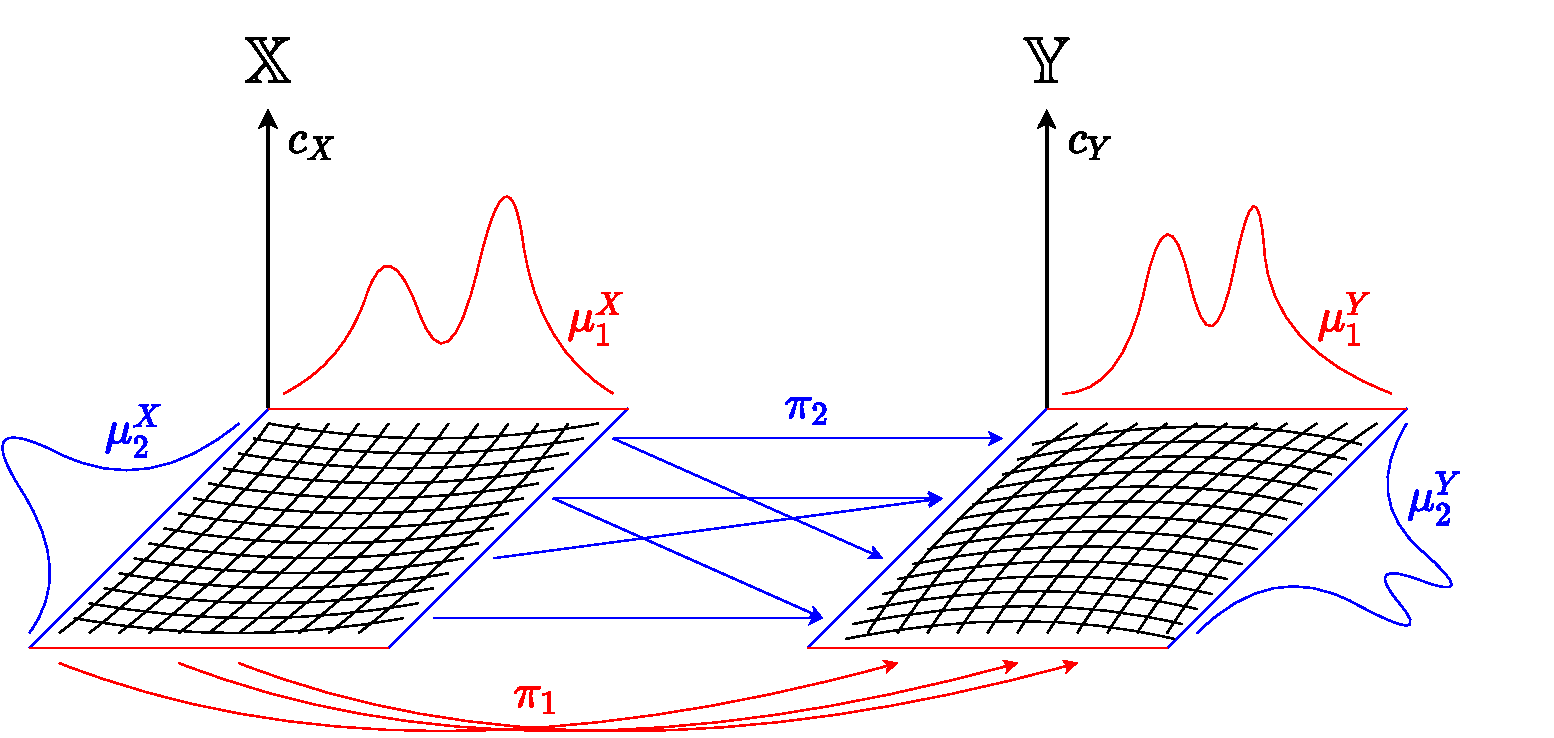
\includegraphics[width=0.9\textwidth, keepaspectratio]{./Chapitre2/fig/coot_diagram.pdf}
%   \caption{Scatter plots of MMOT-DC-v1 versus other solvers. In all three plots, the points tend to concentrate around the line $y=x$,
%   which indicates the comparable performance of MMOT-DC-v1. On the other hand, the top-right plot shows the clear superiority of EGW-PGD.}
%   \label{fig:continuous_coot}
% \end{figure}
First, we can show that the COOT problem \eqref{eq:cont_coot} is well defined.
\begin{proposition}[Lemma 35 in \citep{Chowdhury21b}]
  \label{prop:exist_coot}
  The COOT problem always admits a minimizer.
\end{proposition}
We provide the proof in Appendix \ref{annex:cont_coot}.
While the proofs of our result and of Lemma 35 in \citep{Chowdhury21b} use the same proof technique of
Theorem 2.2 in \citep{Chowdhury19}, ours is slightly different. More precisely,
we exploit a different reformulation of COOT, where it can be rewritten as a multi-marginal OT problem
with additional factorization constraint on the coupling. Later, we will see that,
this observation also allows to establish the convergence result of entropic COOT.

%%%%%%%%%%%%%%%%%%%%%%%%%%%%%%%%%%%%%%%%%%
\subsection{Metric properties}

The framework on the GW isomorphism presented in \Cref{subsec:prop_gw}
can be extended immediately to the COOT setting. In particular, while our
presentation is different to that of \citep{Chowdhury21b}, we still come up with the
same metric properties.

%%%%%%%%%%%%%%%%%%%%%%%%%%%%%%%%%%%%%%%%%
\begin{definition}[Relaxed mass splitting]
  A measure hypernetwork $\cZ$ is a \textbf{relaxed mass splitting} (RMS) of a
  measure hypernetwork $\cX$ if there exist two measure-preserving maps
  $\varphi_k: Z_k \to X_k$, for $k=1,2$, such that the pullback equality
  $c_Z = (\varphi_1, \varphi_2)^*c_X$ holds $\mu^Z_1 \otimes \mu_2^Z$-almost everywhere
  in $Z_1 \times Z_2$. We denote $\ms(\cX)$ the set of all mass splittings
  of $\cX$. This pair of maps $(\varphi_1, \varphi_2)$ is also called
  \textbf{basic weak isomorphism} in \citep{Chowdhury21b}.
\end{definition}
We denote $\rms(\cX)$ the set of all relaxed mass splittings of $\cX$. Clearly,
$\cX \in \rms(\cX)$, so $\rms(\cX)$ is not empty.
In particular, for measure networks, if $\cZ \in \ms(\cX)$, then $\cZ \in \rms(\cX)$,
meaning that $\ms(\cX) \subset \rms(\cX)$. Now, we can define the isomorphism between
the measure hypernetworks as follows.
\begin{definition}[COOT-isomorphism] \label{coot_isomorphic}
  Two measure hypernetworks are
  \begin{enumerate}
    \item strongly isomorphic if there exist two \textbf{bijective}
    measure-preserving map from one hypernetwork to the other such that the pullback equality holds
    \textbf{everywhere}.
    \item semi-strongly isomorphic if one is the RMS of the other and vice versa.
    \item weakly isomorphic if they have a common RMS.
  \end{enumerate}
\end{definition}
This is an immediate relaxation of the GW isomorphism. In particular,
in case of measure networks, isomorphism in GW sense implies COOT isormorphism.
The following result summarizes the relations amongst the three types of COOT isomorphism.
%%%%%%%%%%%%%%%%%%%%%%%%%%%%%%%%%%%%%%%%%%%%%%%%
\begin{corollary} \label{prop:strong_weak_iso}
  Given two measure hypernetworks $\cX$ and $\cY$. Consider three statements
  \begin{enumerate}
    \item[(1)] $\cX$ and $\cY$ are strongly isomorphism.
    \item[(2)] $\cX$ and $\cY$ are semi-strongly isomorphism.
    \item[(3)] $\cX$ and $\cY$ are weakly isomorphism.
  \end{enumerate}
  Then, the following relations hold
  \begin{enumerate}
    \item $(1) \implies (2) \implies (3)$.
    \item If $\cX$ and $\cY$ are finite, then $(2) \implies (1)$.
    \item If $\cX$ and $\cY$ are finite such that $|X_k| = |Y_k|$
    and $\mu_k^X, \mu_k^Y$ are uniform distributions, for $k = 1,2$, then
    $(3) \implies (2)$. This means all three forms are equivalent.
  \end{enumerate}
\end{corollary}
%%%%%%%%%%%%%%%%%%%%%%%%%%%%%%%%%%%%%%%%%%%%%%%%
Now, we can characterize the weak isomorphism by
\begin{proposition} \label{prop:coot_iso}
  Two measure hypernetworks $\cX$ and $\cY$ are COOT-weakly isomorphic if and only if
  $\coot(\cX, \cY) = 0$.
\end{proposition}
%%%%%%%%%%%%%%%%%%%%%%%%%%%%%%%%%%%%%%%%%%%%%%%%
\begin{proposition}[Theorem 1 in \citep{Chowdhury21b}] \label{prop:metric_prop}
  $\coot^{1/p}$ defines a metric on the space of measure hypernetworks, up to COOT-weak isomorphism.
\end{proposition}
%%%%%%%%%%%%%%%%%%%%%%%%%%%%%%%%%%%%%%%%%
% \paragraph{Discussion on the setting of mm-space}
% While the measure network can fit in the COOT framework, this is usually not the case for
% the mm-space since the distance function is only measurable in Polish space,
% but not necessarily bounded. However, all previous results on the existence of minimizer and
% metric property remain unchanged if one replaces measure hypernetworks by mm-spaces,
% as long as COOT is finite. Moreover,
% \begin{corollary}
% For $p=2$, all forms of COOT isomorphisms are equivalent and
% they are also equivalent to the isomorphism in GW sense.
% \end{corollary}
% This indicates that, both GW distance and COOT can be used to compare isometric objects,
% namely those transformed by reflection, rotation or translation.

%%%%%%%%%%%%%%%%%%%%%%%%%%%%%%%%%%%%%%%%%%%%%%%%
\subsection{Entropic regularization and approximation error}
%%%%%%%%%%%%%%%%%%%%%%%%%%%%%%%%%%%%%%%%%%%%%%%%
Similar to the Wasserstein and GW distances, one can approximate the COOT with entropic regularization.
In this thesis, we are interested in the following formulation of entropic COOT:
for $\varepsilon > 0$,
\begin{align}
  \coot_{\varepsilon} (\cX, \cY) =
  \inf_{\substack{\pi_1 \in U(\mu^X_1, \mu^Y_1) \\
  \pi_2 \in U(\mu^X_2, \mu^Y_2)}} &\iint
  \big\vert c_X(x_1, x_2) - c_Y(y_1, y_2) \big\vert^p \; d\pi_1(x_1, y_1) \; d\pi_2(x_2, y_2) \\
  &+ \varepsilon \; \kl \big( \pi_1 \otimes \pi_2 \vert (\mu^X_1 \otimes \mu^Y_1) \otimes (\mu^X_2 \otimes \mu^Y_2) \big).
\end{align}
Note that, this structure of the KL divergence term is particularly handy to prove all results related to
the entropic COOT. It also bears similarity with the \textit{quadratic divergence}
\citep{Sejourne20} defined by $\kl^{\otimes 2}(\mu, \nu):= \kl(\mu \otimes \mu | \nu \otimes \nu)$,
which is used to define the unbalanced GW divergence. Note that, in the balanced setting,
the joint penalization in terms of KL divergence is in fact equivalent to the
independent KL-penalization. More precisely, given any $\pi_k \in U(\mu_k^X, \mu_k^Y)$,
for $k=1,2$, we have
\begin{equation}
  \kl \big( \pi_1 \otimes \pi_2 \vert (\mu^X_1 \otimes \mu^Y_1) \otimes (\mu^X_2 \otimes \mu^Y_2) \big)
  = \kl(\pi_1 \vert \mu^X_1 \otimes \mu^Y_1) + \kl(\pi_2 \vert \mu^X_2 \otimes \mu^Y_2).
\end{equation}
In practice, since the couplings may not have the same nature (for example,
when working directly with the input data, rather than via the similarity matrix),
they can be penalized by different values of regularization.
%%%%%%%%%%%%%%%%%%%%%%%
\begin{proposition}
The entropic COOT problem always admits a minimizer.
\end{proposition}
%%%%%%%%%%%%%%%%%%%%%%%
One major practical interest of entropic COOT is that, for sufficiently small regularization,
it provides a good proxy for unregularized COOT. To formalize this observation, first,
we need to introduce the following assumption on the measure hypernetwork.
%%%%%%%%%%%%%%%%%%%%%%%%%%%%%
\begin{assumption}
  \label{assump:ent_coot}
  Given a measure hypernetwork, we assume that
  \begin{enumerate}
    \item[A1] The sample and feature spaces are finite-dimensional vector spaces.
    \item[A2] Their associated Borel probability measures are absolutely continuous
    with respect to the Lebesgue measure.
  \end{enumerate}
\end{assumption}
%%%%%%%%%%%%%%%%%%%%%%%%%%%%%%
\begin{proposition} \label{prop:conv_ent_coot}
  Under \Cref{assump:ent_coot}, if the interactions are continuous, then
  $\coot_{\varepsilon}(\cX, \cY) \to \coot(\cX, \cY)$ when $\varepsilon \to 0$. Moreover,
  let $(\varepsilon_n)_{n \in \bbN}$ be a sequence of
  positive regularizations such that $\varepsilon_n \to 0$.
  Denote $\pi_n := (\pi_{1, n}, \pi_{2, n})$ the solution of the entropic problem
  $\coot_{\varepsilon_n} (\cX, \cY)$. Then, any cluster point of the sequence $(\pi_n)_n$ is
  a solution of the unregularized COOT problem.
\end{proposition}
%%%%%%%%%%%%%%%%%%%%%%%%%%%%%%
The above result is similar to the one known in entropic OT \citep{Carlier17}. This is due to the fact
that the entropic COOT can be reformulated as a variant of multi-marginal OT problem,
thus the block approximation and $\Gamma$-convergence techniques can be applied.

Furthermore, still under \Cref{assump:ent_coot}, if the measure network is bounded,
then we can quantify the approximation error as follows.
%%%%%%%%%%%%%%%%%%%%%%%%%%%%%%
\begin{proposition} \label{prop:quant_bound_ent}
  Given two measure networks $\cX = (X, \mu_X, c_X)$ and $\cY = (Y, \mu_Y, c_Y)$.
  Suppose that $X$ is bounded subset of $\bbR^{d_x}$ and $Y$ is a bounded subset
  of $\bbR^{d_y}$, where $\diam(X), \diam(Y) \leq D$.
  Denote $d = \max(d_x, d_y)$. Suppose there exists a constants $q > 0$ such that
  $c_X(x_1, x_2) = \vert\vert x_1 - x_2 \vert\vert^q$, for every $(x_1,x_2) \in X^2$, and
  $c_Y(y_1, y_2) = \vert\vert y_1 - y_2 \vert\vert^q$, for every $(y_1,y_2) \in Y^2$. Then,
  \begin{equation}
    \coot_{\varepsilon}(\cX, \cY) - \coot(\cX, \cY) \leq
    \frac{2d \varepsilon}{pq} \log\Big( \frac{pq (2D d^{1/p})^{pq}}{2d \varepsilon} \Big).
  \end{equation}
\end{proposition}
%%%%%%%%%%%%%%%%%%%%%%%%%
This bound is very similar to the one in Wasserstein setting \citep{Genevay19}.
Let us consider two special cases of \Cref{prop:quant_bound_ent}.
\begin{itemize}
  \item[$\bullet$] When $p=2$ and $c_X, c_Y$ are Euclidean distances (\ie, $q=1$),
  the upper bound becomes $d\varepsilon \log\Big( \frac{4D^2}{\varepsilon} \Big)$.

  \item[$\bullet$] When $p=2$ and $c_X, c_Y$ are squared Euclidean distances
  (\ie, $q=2$), the upper bound becomes
  $\frac{d\varepsilon}{2} \log\Big( \frac{32dD^4}{\varepsilon} \Big)$.
\end{itemize}
In both situations, the dependence of the bound on the maximal distance $D$ between points
within each space (even only at logarithmic scale) and on the dimension $d$ indicates
that either high dimensional space, or large intra-space distance (for example, due to outliers)
can have negative impact on the approximation error. On the other hand,
by comparing these two bounds, we deduce that if $\log(2d \varepsilon) \leq 1$,
then the squared Euclidean distances generates a provably better (smaller) upper bound.

With little modification of the proof, exactly the same upper bound in \Cref{prop:quant_bound_ent}
holds for GW distance. We note that \citet{Zhang23} also establish a similar
$O(\varepsilon \log \varepsilon)$-approximation error between the unregularized and entropic GW,
but they rely on different assumptions to ours. In particular, their result only holds
for $2$-GW distance, when the distance function is the squared-Euclidean norm. By contrast,
\Cref{prop:quant_bound_ent} holds for any $p$-GW distance and any $L^q$-norm as distance function.

%%%%%%%%%%%%%%%%%%%%%%%%%%%%%%%%%%%%%%
\section{Factored couplings in Multi-marginal Optimal
Transport via Difference of Convex programming} \label{subsec:MMOT_DC}

%%%%%%%%%%%%%%%%%%%%%%%%%%%%%%%%%%%%%%%
\subsection{Introduction}

Broadly speaking, the classic OT problem provides a principled approach for transporting one probability distribution onto another
following the principle of the least effort. Such a problem, and the distance on the space of probability distributions derived from it,
arise in many areas of machine learning (ML) including generative modeling, transfer learning and information retrieval, where OT has
been successfully applied. A natural extension of classic OT, in which the admissible transport plan can have more
than two prescribed marginal distributions, is called the multi-marginal optimal transport (MMOT) \citep{Gangbo98}.
The latter has several attractive properties: it enjoys a duality theory \citep{Kellerer84} and finds connections with the
probabilistic graphical models \citep{Haasler20} and the Wasserstein barycenter problem \citep{Agueh11} used for data averaging.
While being less popular than the classic OT with two marginals, MMOT is a very useful framework on its own with some notable recent
applications in generative adversarial networks \citep{Cao19}, clustering \citep{Mi21} and domain adaptation
\citep{HuiLCHY18,HeZKSC19}, to name a few.

The recent success of OT in ML is often attributed to the entropic regularization \citep{Cuturi13} where the authors imposed a
constraint on the coupling matrix forcing it to be closer to the independent coupling given by the rank-one product of the marginals.
Such a constraint leads to the appearance of the strongly convex entropy term in the objective function and allows the entropic
OT problem to be solved efficiently using simple Sinkhorn-Knopp matrix balancing algorithm. In addition to this, it was also noticed
that structural constraints on the coupling and cost matrices allow to reduce the high computational cost and sample complexity
of the classic OT problem \citep{Genevay19,Forrow18,Chiheng21,Meyer21a}. However, none of these works considered a much more
challenging case of doing so in a multi-marginal setting. On the other hand, while the work of \citet{Haasler20} considers the MMOT
problem in which the cost tensor induced by a graphical structure, it does not naturally promote the factorizability of
transportation plans.

\paragraph{Contributions} In this work, we define and study a general MMOT problem with structural penalization on the coupling matrix.
We start by showing that a such formulation includes several popular OT methods as special cases and allows to gain deeper insights
into them. We further consider a relaxed problem where the hard constraint is replaced by a regularization term and show that it leads
to an instance of the difference of convex programming problem. A numerical study of the solutions obtained when solving the latter
in cases of interest highlights their competitive performance when compared to solutions provided by the optimization
strategies used previously.

%%%%%%%%%%%%%%%%%%%%%%%%%%%%%%%%%%%%%
\subsection{Preliminary knowledge}

\paragraph{Notations.} For each integer $n \geq 1$, we write $[n] := \{1,...,n\}$.
We denote $\langle \cdot, \cdot \rangle$ denotes the Frobenius inner product.
The generalized Kullback-Leibler divergence between two positive vectors $p, q \in \bbR^n_{> 0}$
is defined as $\kl(p | q) = \sum_i p_i \log \frac{p_i}{q_i} - \sum_i p_i + \sum_i q_i$,
with the convention that $0 \log 0 = 0$.

In what follows, given an integer $N \geq 1$, for any positive integers $a_1,..., a_N$, we call
$P \in \bbR^{a_1 \times ... \times a_N}$ a $N$-D tensor. In particular, a $1$-D tensor is a vector and $2$-D tensor is a matrix.
A tensor is a probability tensor if its entries are nonnegative and the sum of all entries is $1$.
Given $N$ probability vectors $\mu_1, ..., \mu_N$, we write $\mu = (\mu_n)_{n=1}^N$
and $\mu^{\otimes} := \mu_1 \otimes ... \otimes \mu_N$.
We denote $\Sigma$ the set of $N$-D probability tensors and $U(\mu) \subset \Sigma$ the set of nonnegative tensors whose $N$
marginal distributions are $\mu_1, ..., \mu_N$. In this case, any coupling in $U(\mu)$ is said to be \textit{admissible}.

\paragraph{Multi-marginal OT problem.} Given a collection of $N$ probability vectors $\mu = (\mu_n \in \bbR^{a_n})_{n=1}^N$
and a $N$-D cost tensor $C \in \bbR^{a_1 \times ... \times a_N}$, the MMOT problem reads
\begin{equation*}
  \mmot(\mu) = \inf_{P \in U(\mu)} \langle C, P \rangle.
\end{equation*}
In practice, such a formulation is intractable to optimize in a discrete setting as it results in a linear program where the number
of constraints grows exponentially in $N$. A more tractable strategy for solving MMOT is to consider the following entropic
regularization problem
\begin{equation} \label{MMOT_primal}
  \inf_{P \in U(\mu)} \langle C, P \rangle + \varepsilon \kl(P | \mu^{\otimes}).
\end{equation}
which can be solved using Sinkhorn's algorithm \citep{Benamou14}.
We refer the interested reader to Appendix \ref{appendix:subsec_mmot_dc} for algorithmic details.

%%%%%%%%%%%%%%%%%%%%%%%%%%%%%%%%%%%%%%%%%%%%%%%%%
\subsection{Factored Multi-marginal Optimal Transport}

In this section, we first define a factored MMOT (F-MMOT) problem where we seek to promote a structure on the optimal coupling
given such as a factorization into a tensor product. Interestingly, such a formulation can be shown to include several other
OT problems as special cases. Then, we introduce a relaxed version called MMOT-DC where the factorization constraint is
smoothly promoted through a Kullback-Leibler penalty.

\subsubsection{Motivation}

Before a formal statement of our problem, we first give a couple of motivating examples showing
why and when structural constraints on the coupling matrix can be beneficial. To this end,
first note that a trivial example of the usefulness of such constraints in OT is the famous
entropic regularization. Indeed, while most of the works define the latter by adding
negative entropy of the coupling to the classic OT objective function directly,
the original idea was to constraint the sought coupling to remain close (to some extent)
to a rank-one product of the two marginal distributions. The appearance of negative entropy
in the final objective function is then only a byproduct of such constraint due to
the decomposition of the KL divergence into a sum of three terms with two of them being constant.
Below we give two more examples of real-world applications related to MMOT problem
where a certain decomposition imposed on the coupling tensor can be desirable.
\paragraph{Multi-source multi-target translation.} A popular task in computer vision is
to match images across different domains in order to perform the so-called image translation.
Such tasks are often tackled within the GAN framework where one source domain from which
the translation is performed, is matched with multiple target domains modeled using generators.
While MMOT was applied in this context by \citet{Cao19} when only one source was considered,
its application in a multi-source setting may benefit from structural constraints
on the coupling tensor incorporating the human prior on what target domains each source domain
should be matched to.

\paragraph{Multi-task reinforcement learning.} In this application, the goal is to learn
individual policies for a set of agents while taking into account the similarities between them
and hoping that the latter will improve the individual policies. A common approach is
to consider an objective function consisting of two terms where the first term is concerned
with learning individual policies, while the second forces a consensus between them.
Similar to the example considered above, MMOT problem was used to promote the consensus
across different agents' policies in \citep{Cohen21}, even though such a consensus
could have benefited from a prior regarding the semantic relationships between the learned tasks.
%
%We can cite other examples motivating the introduction of structural constraints in MMOT problem but the bottom line of it remains unchanged: imposing a certain structure on the optimal coupling tensor is a way of incorporating the human-based priors to the MMOT problem that reflect the domain knowledge about the problem at hand. We now proceed to the formal introduction of this idea.

\subsubsection{Factored MMOT and its relaxation}
We start by giving several definitions used in the following parts of this section.
%We call $P \in \bbR^{a_1 \times ... \times a_N}$ a $N$-D tensor. When $N=1$, we simply call it a vector and when $N=2$,
%it is a matrix.
\begin{definition}[Tuple partition]
 Given two integers $N \geq M \geq 2$, a sequence of tuples $\cT = (\cT_m)_{m=1}^M$, is called a
 \underline{tuple partition} of the $N$-tuple $(1,...,N)$ if the tuples $\cT_1, ..., \cT_M$ are nonempty and disjoint,
 and their concatenation in this order gives $(1,...,N)$.
\end{definition}
Here, we implicitly take into account the order of the tuple, which is not the case for the partition of the set $[N]$. If
there exists a tuple in $\cT$ which contains only one element, then we say $\cT$ is \textit{degenerate}.

\begin{definition}[Marginal tensor]
  Given a tensor $P \in \bbR^{a_1 \times ... \times a_N}$ and a tuple partition $\cT = (\cT_m)_{m=1}^M$,
  we call $P_{\# \cT_m}$ its \underline{$\cT_m$-marginal tensor}, by summing $P$ over all dimensions not in $\cT_m$.
  We write $P_{\# \cT} = P_{\# \cT_1} \otimes ... \otimes P_{\# \cT_M} \in \bbR^{a_1 \times ... \times a_N}$
  the tensor product of its marginal tensors.
\end{definition}
For example, for $M=N=2$, we have $\cT_1 = (1)$ and $\cT_2 = (2)$. So, given a matrix
$P \in \bbR^{a_1 \times a_2}$, its marginal tensors $P_{\# \cT_1}$ and $P_{\# \cT_2}$ are simply vectors in
$\bbR^{a_1}$ and $\bbR^{a_2}$, respectively, defined by $(P_{\# \cT_1})_i = \sum_j P_{ij}$ and
$(P_{\# \cT_2})_j = \sum_i P_{ij}$ for $(i,j) \in [a_1] \times [a_2]$. The tensor product
$P_{\# \cT} \in \bbR^{a_1 \times a_2}$ is then defined by
$(P_{\#\cT})_{ij} = (P_{\# \cT_1})_i (P_{\# \cT_2})_j$.
Clearly, if $P$ is a probability tensor, then so are its marginal tensors and tensor product.

Suppose $\cT_m = (p,...,q)$ for some $m \in [M]$ and $1 \leq p \leq q \leq N$. We denote
$\Sigma_{\cT_m}$ the set of probability tensors in $\bbR^{a_p \times ... \times a_q}$ and
$U_{\cT_m} \subset \Sigma_{\cT_m}$ the set
of probability tensors in $\bbR^{a_p \times ... \times a_q}$ whose
$r^{\text{th}}$-marginal vector is $\mu_r$, for every $r = p,...,q$.
We also define $\mu^{\otimes}_{\cT_m} := \mu_p \otimes ... \otimes \mu_q$.

%%%%%%%%%%%%%%%%%%%%%%%%%%%%%%%
\begin{definition}[Factored MMOT]
  Given a collection of histograms $\mu = (\mu_n)_{n=1}^N$ and a tuple partition $\cT = (\cT_m)_{m=1}^M$,
  we consider the following OT problem
  \begin{equation} \label{factor_mmot}
    \fmmot( \cT, \mu) = \inf_{P \in U_{\cT}} \langle C, P \rangle,
  \end{equation}
  where $U_{\cT} \subset U(\mu)$ is the set of admissible couplings which can be factorized as a tensor product of $M$
  component probability tensors in $\Sigma_{\cT_1}, ..., \Sigma_{\cT_M}$.
\end{definition}
Several remarks are in order here. First, one should note that the partition considered above is in general not degenerate meaning
that the decomposition can involve tensors of an arbitrary order $<N$. Second, the decomposition in this setting depicts the prior
knowledge regarding the tuples of measures which should be independent: the couplings for the measures from different tuples will
be degenerate and the optimal coupling tensor will be reconstructed from couplings of each tuple separately.
Third, suppose the partition $(\cT_m)_{m=1}^M$ is not degenerate and $M=2$, i.e. the tensor is factorized as product of
two tensors, Problem \eqref{factor_mmot} is equivalent to a variation of low non-negative rank OT problem
(see Appendix \ref{appendix:subsec_mmot_dc}).

As for the existence of the solution to this problem, we have that $U_{\cT}$ is compact because it is a close subset of the
compact set $U(\mu)$, which implies that Problem \eqref{factor_mmot} always admits a solution. Furthermore, observe that
\begin{equation}
  \begin{split}
    U_{\cT} &= \{ P \in U(\mu): P = P_1 \otimes ... \otimes P_M, \text{where } P_m \in \Sigma_{\cT_m}, \forall m = 1,...,M \} \\
    &= \{ P \in \Sigma: P = P_1 \otimes ... \otimes P_M, \text{where } P_m \in U_{\cT_m}, \forall m = 1,...,M \}.
  \end{split}
\end{equation}
Thus, the problem F-MMOT can be rewritten as
\begin{equation}
  \fmmot( \cT, \mu) = \inf_{\substack{P_m \in U_{\cT_m} \\ \forall m = 1,...,M}}
  \langle C, P_1 \otimes ... \otimes P_M \rangle.
\end{equation}
So, if $\cT_1,...,\cT_M$ are $2$-tuples and two marginal distributions corresponding to each $U_{\cT_m}$ are
identical and uniform, then by Birkhoff's theorem \citep{Birkhoff46}, Problem \eqref{factor_mmot} admits an optimal solution in
which each component tensor $P_m$ is a permutation matrix.

\paragraph{Two special cases.} When $N = 4$ and $M=2$ with $\cT_1 = (1,2)$ and $\cT_2 = (3,4)$, Problem
\eqref{factor_mmot} becomes the CO-Optimal transport (COOT), where the two component tensors are known as
\textit{sample} and \textit{feature} couplings. If furthermore, $a_1 = a_3, a_2=a_4$, and $\mu_1 = \mu_3, \mu_2=\mu_4$, it becomes a
lower bound of the discrete Gromov-Wasserstein (GW) distance. This means that our formulation can be seen as a
generalization of several OT formulations.

%%%%%%%%%%%%%%%%%%%%%%%%%%%%%%%%%%%%%%%%%%%%%
Observe that if a probability tensor $P$ can be factorized as a tensor product of probability tensors, i.e.
$P = P_1 \otimes ... \otimes P_M$, then each $P_m$ is also the $\cT_m$-marginal tensor of $P$. In this case,
we have $P = P_{\# \cT}$. This prompts us to consider the following relaxation of factored MMOT, where the hard constraint
$U_{\cT}$ is replaced by a regularization term.
\begin{definition}[Relaxed Factored MMOT]
  Given $\varepsilon \geq 0$, a collection of measures $\mu$ and a tuple partition $\cT$,
  we define the following problem:
  \begin{equation} \label{relax_mmot}
    \mmotdc_{\varepsilon}( \cT, \mu) =
    \inf_{P \in U(\mu)} \langle C, P \rangle + \varepsilon \kl(P \vert P_{\# \cT}).
  \end{equation}
\end{definition}
From the exposition above, one can guess that this relaxation is reminiscent of the entropic regularization in MMOT and
coincides with it when $M = N$. As such, it also recovers the classical entropic OT. One should note that the choice of the KL
divergence is not arbitrary and its advantage will become clear when it comes to the algorithm. %A well known
A special case of Problem \eqref{relax_mmot} is when $M = N$, we recover the entropic-regularized MMOT problem.

After having defined the two optimization problems, we now set on exploring their theoretical properties.

%%%%%%%%%%%%%%%%%%%%%%%%%%%%%%%%%%%%%%%%%%%%%%%
\subsection{Theoretical properties}
Intuitively, the relaxed problem is expected to allow for solutions with a lower value of the final objective function. We formally prove the validity of this intuition below.
%%%%%%%%%%%%%%%%%%%%%%%%%%%%%%%%%%%%%%%%%%%%%
\begin{proposition}[Preliminary properties]
  \label{MMOT_dc_prop}
  Given a collection of histograms $\mu$ and a tuple partition $\cT$,
  \begin{enumerate}
    \item For every $\varepsilon \geq 0$, we have $\mmot(\mu) \leq
    \mmotdc_{\varepsilon}(\cT, \mu) \leq \fmmot( \cT, \mu)$.
    \item For every $\varepsilon > 0, \mmotdc_{\varepsilon}( \cT, \mu ) = 0$ if and only if
    $\fmmot (\cT, \mu) = 0$.
  \end{enumerate}
\end{proposition}
%%%%%%%%%%%%%%%%%%%%%%%%%%%%%%%%%%%%%%%%%%%%%
An interesting property of MMOT-DC is that it interpolates between MMOT and F-MMOT. Informally,
for very large $\varepsilon$, the KL divergence term dominates, so the optimal transport plans tend to be factorizable.
On the other hand, for very small $\varepsilon$, the KL divergence term becomes negligible and we approach MMOT.
The result below formalizes this intuition.
%%%%%%%%%%%%%%%%%%%%%%%%%%%%%%%%%%%%%%%%%%%%%
\begin{proposition}[Interpolation between MMOT and F-MMOT]
  \label{interpolation_prop}
  For any tuple partition $\cT$ and for $\varepsilon > 0$,
  let $P_{\varepsilon}$ be a minimiser of the problem $\mmotdc_{\varepsilon}(\cT, \mu)$.
  \begin{enumerate}
    \item When $\varepsilon \to \infty$, one has $\mmotdc_{\varepsilon}(\cT, \mu) \to
    \fmmot(\cT, \mu)$. In this case, any cluster point of the sequence of minimisers
    $(P_{\varepsilon})_{\varepsilon}$ is a minimiser of $\fmmot(\cT, \mu)$.

    \item When $\varepsilon \to 0$, then $\mmotdc_{\varepsilon}(\cT, \mu) \to \mmot(\mu)$.
    In this case, any cluster point of the sequence of minimisers $(P_{\varepsilon})_{\varepsilon}$ is a minimiser of
    $\mmot(\mu)$.
  \end{enumerate}
\end{proposition}
%%%%%%%%%%%%%%%%%%%%%%%%%%%%%%%%%%%%%%%%%%%%%
\paragraph{GW distance revisited.} Somewhat surprisingly, the relaxation \eqref{relax_mmot} also allows us to prove the equality
between GW distance and COOT in the discrete setting. Let $\cX$ be a
finite subset (of size $m$) of a certain metric space. Denote $C_x \in \bbR^{m \times m}$ its similarity matrix (e.g. distance
matrix). We define similarly the set $\cY$ of size $n$ and the corresponding similarity matrix $C_y \in \bbR^{n \times n}$.
We also assign two discrete probability measures $\mu_x \in \bbR^m$ and $\mu_y \in \bbR^n$ to $\cX$ and $\cY$,
respectively. The GW distance is then defined as
\begin{equation}
  \gw(C_x, C_y) = \inf_{Q \in U(\mu_x, \mu_y)} \langle L(C_x, C_y), Q \otimes Q \rangle,
\end{equation}
and the COOT reads
\begin{equation}
  \coot(C_x, C_y) = \inf_{\substack{Q_s \in U(\mu_x, \mu_y) \\ Q_f \in U(\mu_x, \mu_y)}}
  \langle L(C_x, C_y), Q_s \otimes Q_f \rangle,
\end{equation}
where $L(C_x,C_y) \in \bbR^{m \times n \times m \times n}$ represents the $4$-D cost tensor induced by the matrices $C_x$ and $C_y$,
and $U(\mu, \nu)$ is the set of couplings in $\bbR^{m \times n}_{\geq 0}$ whose two marginal distributions are $\mu$ and
$\nu$. When $C_x$ and $C_y$ are two squared Euclidean distance matrices, and $L(C_x,C_y)$ is of the form
$\big(L(C_x,C_y)\big)_{i,j,k,l} = \vert (C_x)_{i,k} - (C_y)_{j,l} \vert^2$, it can be shown that the GW distance is equal
to the COOT. This is also true when $L(C_x, C_y)$ is a negative definite kernel \citep{Sejourne20}.
Here, we establish a weaker case where this equality still holds.
%%%%%%%%%%%%%%%%%%%%%%%%%%%%%%%%%%%%%%%%%%%%%
\begin{corollary} \label{kernel_gw_coot}
  If $L(C_x, C_y)$ defines a conditionally negative definite kernel on $(\cX \times \cY)^2$, then we have the equality
  between GW distance and COOT. Furthermore, if $(Q_s^*,Q_f^*)$ is a solution of the COOT problem, then $Q_s^*$ and $Q_f^*$ are
  two solutions of the GW problem. In particular, when $L(C_x, C_y)$ induces a strictly positive definite kernel
  $\exp \big( -\frac{L(C_x, C_y)}{\varepsilon} \big)$, for every $\varepsilon > 0$, we have $Q_s^* = Q_f^*$.
\end{corollary}
%%%%%%%%%%%%%%%%%%%%%%%%%%%%%%%%%%%%%%%%%%%%%
The proof relies on the connection between MMOT-DC and COOT shown in \Cref{interpolation_prop},
and given a $4$-D solution of MMOT-DC, we can construct another $4$-D solutions whose
$\cT_1$ and $\cT_2$-marginal matrices are identical,
under the assumption of the cost tensor. The proof of the second claim is deferred to the
Appendix \ref{appendix:subsec_mmot_dc}.

%%%%%%%%%%%%%%%%%%%%%%%%%%%%%%%%%%%%%%%%%%%%%%%%%%%%%ù
\subsection{Numerical solution} \label{sec:algo}
%%%%%%%%%%%%%%%%%%%%%%%%%%%%%%%%%%%%%%%%%%%%%
We now turn to the computational aspect of Problem \eqref{relax_mmot}. First, note that for any tuple partition
$\cT = (\cT_m)_{m=1}^M$ and probability tensor $P$, the KL divergence term can be decomposed as
\begin{equation}
  \kl(P \vert P_{\# \cT}) = \kl(P | \mu^{\otimes}) - \sum_{m=1}^m \kl_m(P),
\end{equation}
where the function $\kl_m$ defined by $\kl_m(P) := \kl(P_{\# \cT_m} | \mu^{\otimes}_{\cT_m})$
is continuous and convex with respect to $P$. Now, Problem \eqref{relax_mmot} becomes
\begin{equation} \label{relax}
  \mmotdc_{\varepsilon}(\cT, \mu) = \inf_{P \in U(\mu)}
  \langle C, P \rangle + \varepsilon \kl(P | \mu^{\otimes}) - \varepsilon \sum_{m=1}^m \kl_m(P).
\end{equation}
This is nothing but a Difference of Convex (DC) programming problem (which explains the name MMOT-DC),
thanks to the convexity of the set $U(\mu)$ and the KL divergence. Thus, it can be solved
by the classic DC algorithm
\footnote{The DC algorithm is very closely related to Convex-concave procedure,
majorization-minimization algorithm, Successive Linear
Approximation. See \citep{Le18} for more details.} \citep{Tao86,Tao97} as follows:
at the iteration $t$,
\begin{enumerate}
  \item Calculate $G^{(t)} \in \partial(\sum_{m=1}^M \kl_m)(P^{(t)})$.
  \item Solve $P^{(t+1)} \in \argmin_{P \in U(\mu)} \langle C -
  \varepsilon G^{(t)}, P \rangle + \varepsilon \kl(P | \mu^{\otimes})$.
\end{enumerate}
%%%%%%%%%%%%%%%%%%%%%%%%%%%%%%%%%%%%%%%%%%%%%%
This algorithm is very easy to implement. Indeed, the second step is an entropic-regularized MMOT problem, which admits a unique
solution, thanks to the strict convexity of the objective function.
Such solution can be found by the Sinkhorn algorithm
\ref{algo:dual_mmot}. In the first step, the gradient can be calculated explicitly.
For the sake of simplicity, we illustrate the calculation in a simple case, where $M=2$ and $N=4$ with
$\cT_1$ and $\cT_2$ are two $2$-tuples. The function $\kl_1 + \kl_2$ is continuous, so
$G^{(t)} = \nabla_P (\kl_1 + \kl_2)(P^{(t)})$. Given a $4$-D probability tensor $P$, we have
\begin{equation} \label{optim_condition}
  \frac{\partial (\kl_1 + \kl_2)}{\partial P_{i,j,k,l}} =
  \log \left( \frac{\sum_{k,l} P_{i,j,k,l}}{(\mu_1)_i (\mu_2)_j} \right) +
  \log \left( \frac{\sum_{i,j} P_{i,j,k,l}}{(\mu_3)_k (\mu_4)_l} \right).
\end{equation}
The complete DC algorithm for Problem \eqref{relax} can be found in \Cref{algo:dc_MMOT}.
%%%%%%%%%%%%%%%%%%%%%%%%%%%%%%%%%%%%%%%%%%%%%%
\begin{algorithm}[t]
  \caption{DC algorithm for Problem \eqref{relax_mmot}.}
  \textbf{Input.} Cost tensor $C$, tuple partition $(\cT_m)_{m=1}^M$, collection of histograms $\mu = (\mu_n)_{n=1}^N$,
  hyperparameter $\varepsilon > 0$, initialization $P^{(0)}$, tuple of initial dual vectors for the
  Sinkhorn step $(f_1^{(0)},...,f_N^{(0)})$.

  \textbf{Output.} Tensor $P \in U(\mu)$.

  While not converge
  \begin{enumerate}
    \item Gradient step: compute the gradient of the convex term $G^{(t)} = \sum\limits_{m=1}^M \nabla_P \kl_m(P^{(t)})$.
    \item Sinkhorn step: solve
    \begin{equation}
      P^{(t+1)} = \argmin_{P \in U(\mu)} \langle C - \varepsilon G^{(t)}, P \rangle + \varepsilon \kl(P | \mu^{\otimes}),
    \end{equation}
    using the Sinkhorn algorithm \ref{algo:dual_mmot}, with the tuple of initial dual vectors $(f_1^{(0)},...,f_N^{(0)})$.
  \end{enumerate}
  \label{algo:dc_MMOT}
\end{algorithm}

%%%%%%%%%%%%%%%%%%%%%%%%%%%%%%%%%%%%%%%%%%%%%%
\subsection{Experimental evaluation} \label{sec:exp}
%%%%%%%%%%%%%%%%%%%%%%%%%%%%%%%%%%%%%%%%%%%%%%
In this section, we illustrate the use of MMOT-DC on simulated data. Rather than performing experiments in full generality,
we choose the setting where $N = 4$ and $M=2$ with $\cT_1 = (1,2)$ and $\cT_2 = (3,4)$,
so that we can compare MMOT-DC with other popular solvers of COOT and GW distance. Given two matrices $X$ and $Y$, we always consider the $4$-D cost tensor $C$,
where $C_{i,j,k,l} = \vert X_{i,k} - Y_{j,l} \vert^2$. On the other hand, we are not interested in the $4$-D minimiser of MMOT-DC,
but only in its two $\cT_1, \cT_2$-marginal matrices.

\paragraph{Solving COOT on a toy example.} We generate a random matrix $X \in \bbR^{30 \times 25}$, whose entries are drawn independently
from the uniform distribution on the interval $[0,1)$. We equip the rows and columns of $X$ with two discrete uniform distributions
on $[30]$ and $[25]$. We fix two permutation matrices $Q_s \in \bbR^{30 \times 30}$ (called sample permutation) and
$Q_f \in \bbR^{25 \times 25}$ (called feature permutation), then calculate $Y = Q_s X Q_f$. We also equip the rows and columns of $Y$
with two discrete uniform distributions on $[30]$ and $[25]$.

It is not difficult to see that $\coot(X,Y) = 0$ because $(Q_s, Q_f)$ is a solution. As COOT is a special case of F-MMOT,
we see that $\mmotdc_{\varepsilon}(\cT, \mu) = 0$, for every $\varepsilon > 0$,
by \Cref{MMOT_dc_prop}. In this experiment, we will check if marginalizing the minimizer of MMOT-DC allows us to recover
the permutation matrices $Q_s$ and $Q_f$.
As can be seen from \Cref{fig:permu}, MMOT-DC can recover the permutation positions, for various
values of $\varepsilon$. On the other hand, it can not recover the true sparse permutation matrices because the Sinkhorn algorithm
applied to the MMOT problem implicitly results in a dense tensor, thus having dense marginal matrices. For this reason,
the loss only remains very close to zero, but never exactly.
%%%%%%%%%%%%%%%%%%%%%%%%%%%%%%%%%%%%%%%
\begin{figure}[t]
  \centering
  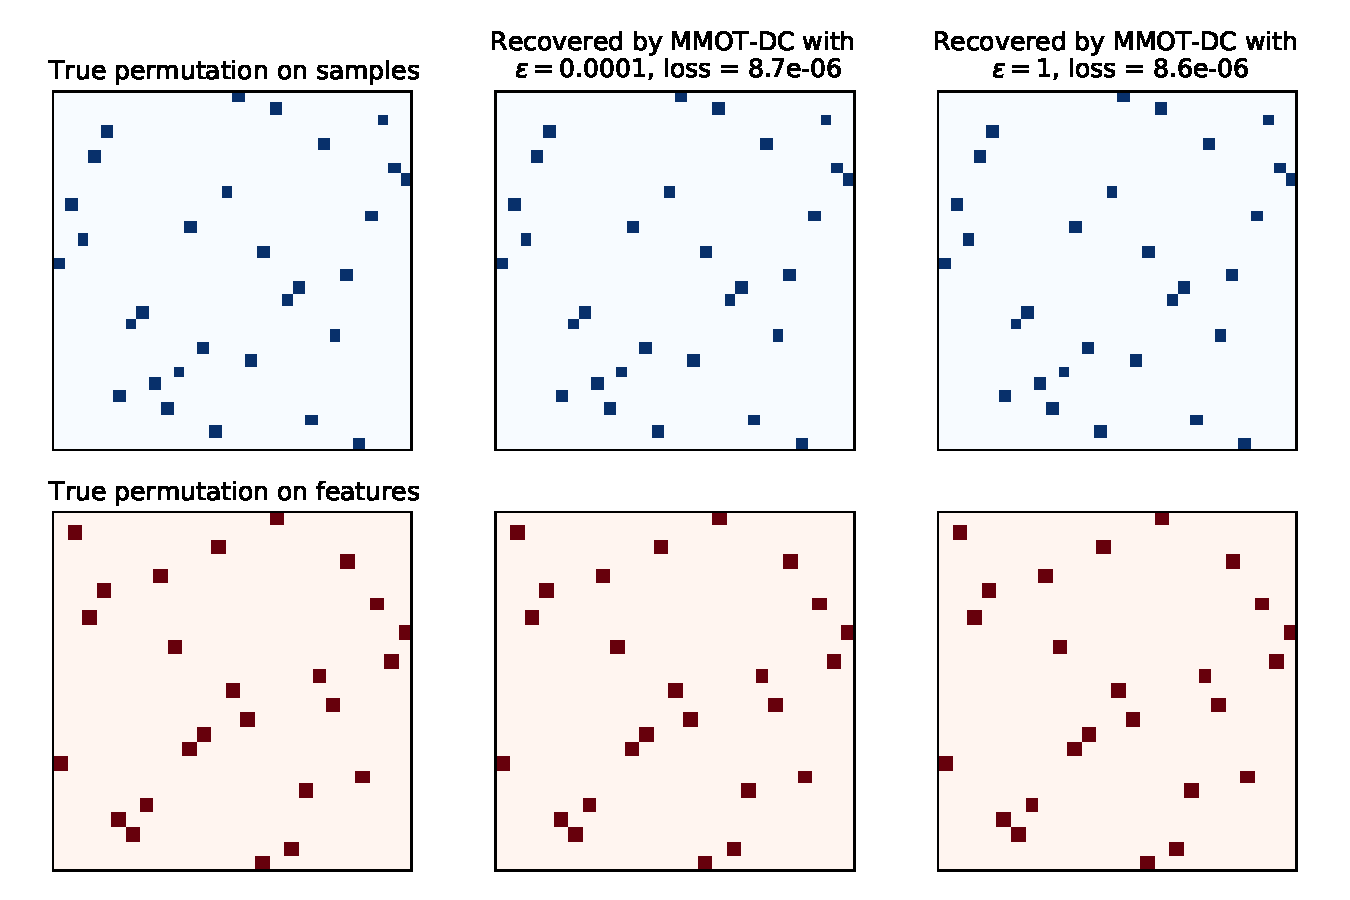
\includegraphics[width=0.8\textwidth,height=0.8\textheight,keepaspectratio]{./Chapitre2/fig/compare_methods.pdf}
  \caption{Couplings generated by COOT and MMOT-DC on the matrix recovering task.}
  \label{fig:permu}
\end{figure}
%%%%%%%%%%%%%%%%%%%%%%%%%%%%%%%%%%%%%%%
We also plot, with some abuse of notation, the histograms of the difference between
the $(1,3), (1,4), (2,3), (2,4)$-marginal matrices of MMOT-DC and their corresponding counterparts from F-MMOT.
In this example, in theory, as the optimal tensor $P$ of F-MMOT can be factorized as
$P = P_{\# \cT_1} \otimes P_{\# \cT_2} = Q_s \otimes Q_f$,
it is immediate to see that $P_{\# (1,3)} = P_{\# (1,4)} = P_{\# (2,3)} = P_{\# (2,4)} \in \bbR^{30 \times 25}$
are uniform matrices whose entries are $\frac{1}{750}$.
%%%%%%%%%%%%%%%%%%%%%%%%%%%%%%%%%%%%%%%
\begin{figure}[t]
  \centering
  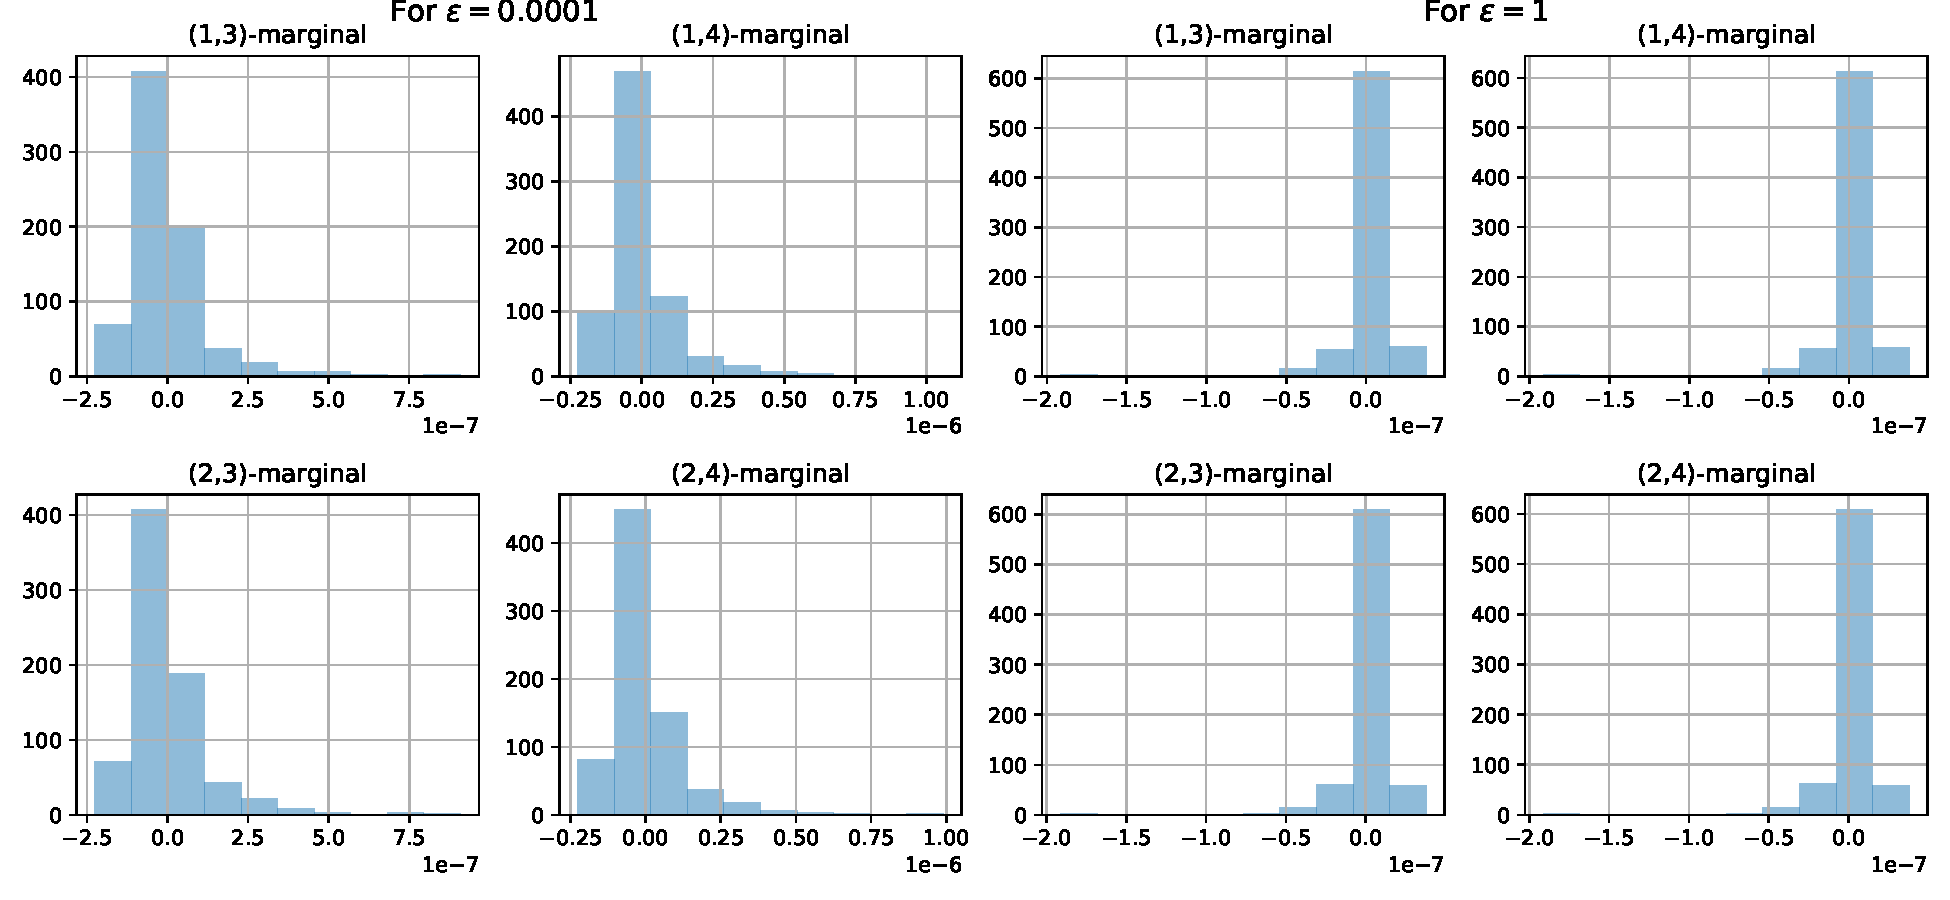
\includegraphics[width=1.\textwidth,height=1.\textheight,keepaspectratio]{./Chapitre2/fig/other_marginals.pdf}
  \caption{Histograms of difference between true independent marginal matrices and their approximations. We see that the marginal matrices obtained
  by \Cref{algo:dc_MMOT} approximate well the theoretical uniform matrices.}
  \label{fig:other_marg}
\end{figure}

%%%%%%%%%%%%%%%%%%%%%%%%%%%%%%%%%%%%%%%
\paragraph{Quality of the MMOT-DC solutions. \label{expe:2}}

% In the following example, our evaluation metric is the COOT loss $\langle C, P \otimes Q \rangle$,
% where the smaller the loss, the better.

Now, we consider the situation where the true matching between two matrices is not known in advance and investigate the quality
of the solutions returned by MMOT-DC to solve the COOT and GW problems. This means that we will look at the COOT loss
$\langle C, Q_s \otimes Q_f \rangle$, where the smaller the loss, the better when using both exact COOT and GW solvers
and our relaxation.

We generate two random matrices $X \in \bbR^{20 \times 3}$ and $Y \in \bbR^{30 \times 2}$,
whose entries are drawn independently from the uniform distribution on the interval $[0,1)$. Then we calculate two corresponding
squared Euclidean distance matrices of size $20$ and $30$. Their rows and columns are equipped with the discrete
uniform distributions. In this case, \citet{Redko20} show that the COOT loss coincides with the GW distance, and the
Block Coordinate Descent (BCD) algorithm used to approximate COOT is equivalent to the Frank-Wolfe algorithm \citep{Frank56}
used to solve the GW distance.

We compare four solvers:
\begin{enumerate}
  \item The Frank-Wolfe algorithm to solve the GW distance (GW-FW).

  \item The projected gradient algorithm to solve the entropic GW distance \citep{Peyre16} (EGW-PGD).
  We choose the regularization parameter from the set
  $\{0.0008, 0.0016, 0.0032, 0.0064, 0.0128, 0.0256 \}$
  and pick the one which corresponds to smallest COOT loss.

  \item The Block Coordinate Descent algorithm to approximate the entropic COOT \citep{Redko20}
  (EGW-BCD), where two additional KL divergences corresponding to two couplings are introduced.

  The regularization parameters are tuned from the set
  $\{0, 0.0005, 0.001, 0.005, 0.01, 0.05, 0.1, 0.5, 1 \}$,
  where $0$ means that there is no regularization term for the corresponding coupling
  and we pick the pair corresponding to the smallest COOT loss.

  \item \Cref{algo:dc_MMOT} to solve the MMOT-DC. We tune
  $\varepsilon \in \{1, 1.4, 1.8, 2.2, 2.6\}$ and we pick the one which corresponds to smallest COOT loss.
\end{enumerate}
For GW-FW and EGW-PGD, we use the implementation from the Python Optimal Transport package \citep{Flamary21}.

Given two random matrices, we record the COOT loss corresponding to the solution generated by each method.
We simulate this process $70$ times and compare their overall performance. We can see in \Cref{tab:gw} the average value and
standard deviation and the comparison for the values of the loss between the different algorithms in \Cref{fig:gw}.
The performance is quite similar across methods with a  slight advantage for EGW-PGD. This is in itself a very
interesting result that has never been noted, to the best of our knowledge: the reason that the entropic version of GW can
provide better solution than solving the exact problem, may be due to the "convexification" of the problem, thanks to the entropic
regularization. Our approach is also interestingly better than the exact GW-FW, which illustrates that the relaxation might help in
finding better solutions despite the non-convexity of the problem.
%%%%%%%%%%%%%%%%%%%%%%%%%%%%%%%%%%%%%%%
\begin{table}[t]
  % \vskip 0.15in
  \begin{center}
    \begin{small}
      \begin{sc}
        \begin{tabular}{|c|c|c|c|}
          \hline
          GW-FW & EGW-PGD & EGW-BCD & MMOT-DC \\
          \hline
          0.0829 ($\pm$ 0.0354) & \textbf{0.0786 ($\pm$ 0.0347)} & 0.0804 ($\pm$ 0.0353) & 0.0822 ($\pm$ 0.0364) \\
          \hline
        \end{tabular}
      \end{sc}
    \end{small}
  \end{center}
  \caption{Average and standard deviation of COOT loss of the solvers. MMOT-DC is competitive to other solvers,
  except for EGW-PGD and EGW-BCD.
  \label{tab:gw}}
\end{table}

%%%%%%%%%%%%%%%%%%%%%%%%%%%%%%%%%%%%%%%
\begin{figure}[t]
	\centering
	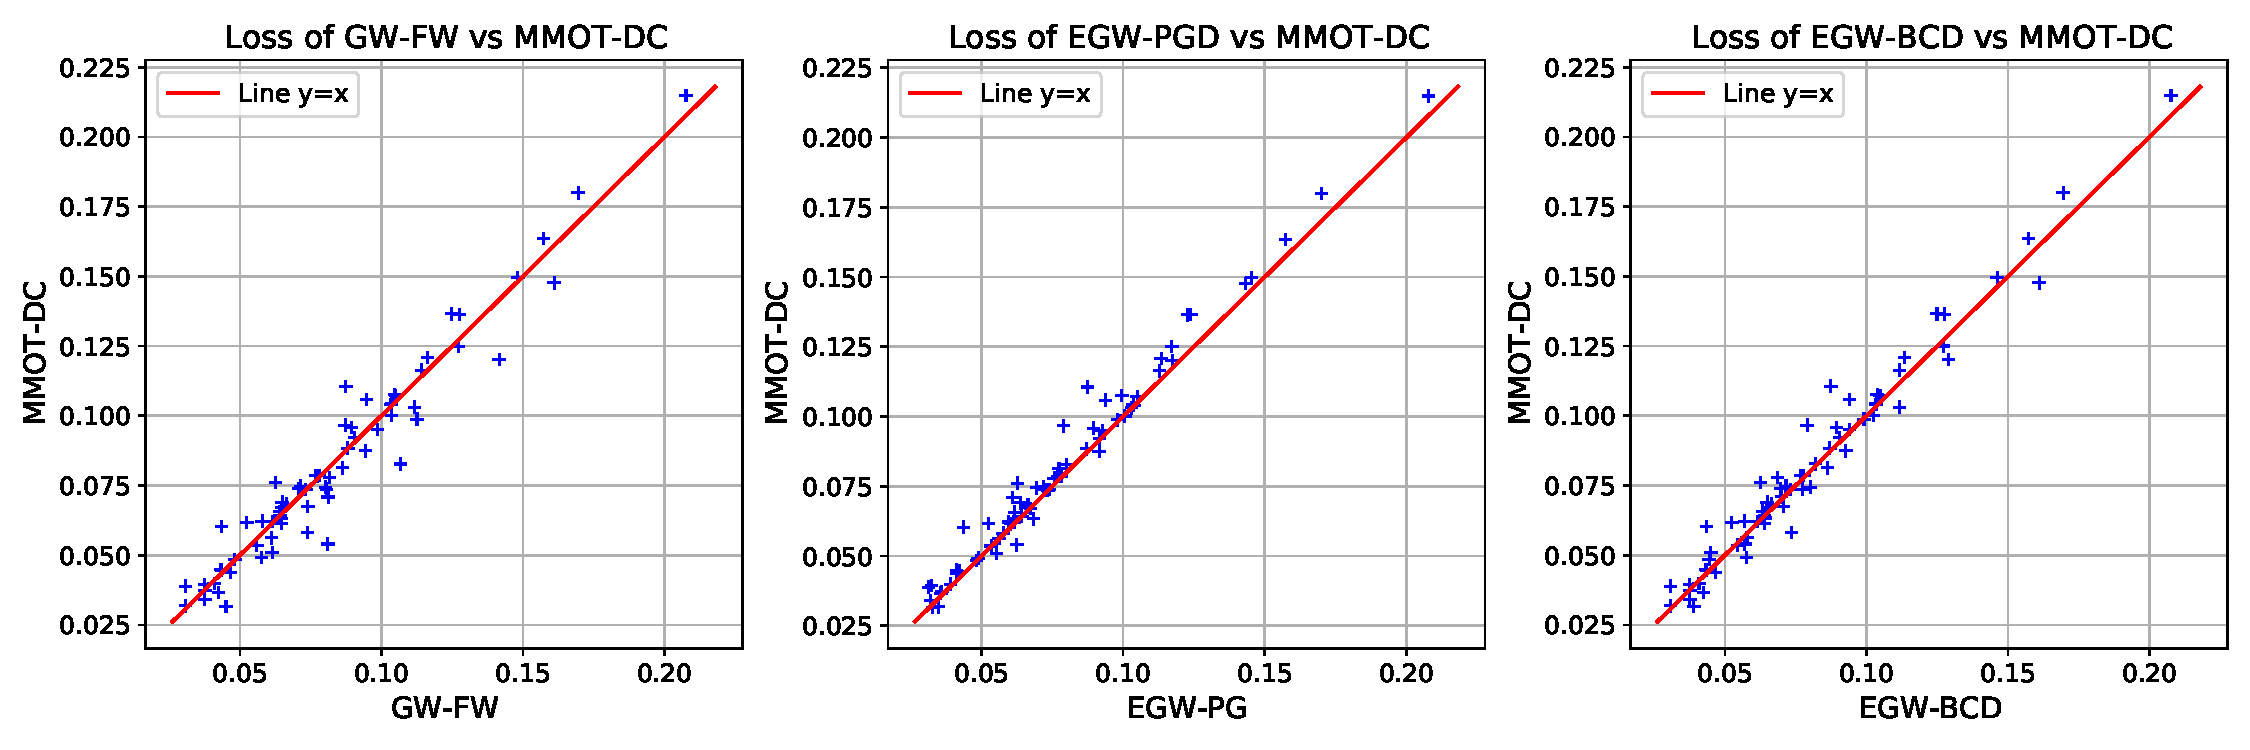
\includegraphics[width=\textwidth,height=\textheight,keepaspectratio]{./Chapitre2/fig/all_vs_MMOT-DC.pdf}
	\caption{Scatter plots of MMOT-DC versus other solvers. In all three plots, the points tend to concentrate around the line $y=x$,
  which indicates the comparable performance of MMOT-DC. On the other hand, the top-right plot shows the clear superiority of EGW-PGD.}
	\label{fig:gw}
\end{figure}
%%%%%%%%%%%%%%%%%%%%%%%%%%%%%%%%%%%%%%%

\paragraph{An empirical variation.} Intuitively, for sufficiently large $\varepsilon$, the minimisation of the KL divergence is prioritised
over the linear term in the objective function of the MMOT-DC problem, which implies that the optimal tensor $P^*$ is "close" to its
corresponding tensor product $P^*_{\# \cT}$. So, instead of calculating the gradient at $P$, one may calculate at
$P_{\# \cT}$. In this case, the gradient reads
\begin{equation}
  \begin{split}
    \sum_{m=1}^M \nabla_P \kl_m(P_{\# \cT}) =
    \log \frac{P_{\# \cT_1}}{\mu^{\otimes}_{\cT_1}} \oplus ... \oplus \log \frac{P_{\# \cT_m}}{\mu^{\otimes}_{\cT_m}} ,
  \end{split}
\end{equation}
where $\oplus$ represents the tensor sum operator between two arbitrary-size tensors: $(A \oplus B)_{i,j}:= A_i + B_j$, where with some
abuse of notation, $i$ or $j$ can be understood as a tuple of indices. Thus, we avoid storing the $N$-D gradient tensor (as in the
\Cref{algo:dc_MMOT}) and only need to store $M$ smaller-size tensors. Not only saving the memory,
this variation also seems to be empirically competitive with the original \Cref{algo:dc_MMOT}, if not sometimes better,
in terms of COOT loss. The underlying reason might be related to the approximate DCA scheme \citep{Thanh15}, where one replaces both
steps in each DC iteration by their approximation. We leave the formal theoretical justification of this variation to the future work.
We call this variation \textit{MMOT-DC-v1} and use the same setup as in Experiment \ref{expe:2}.
\begin{figure}[ht]
  \centering
  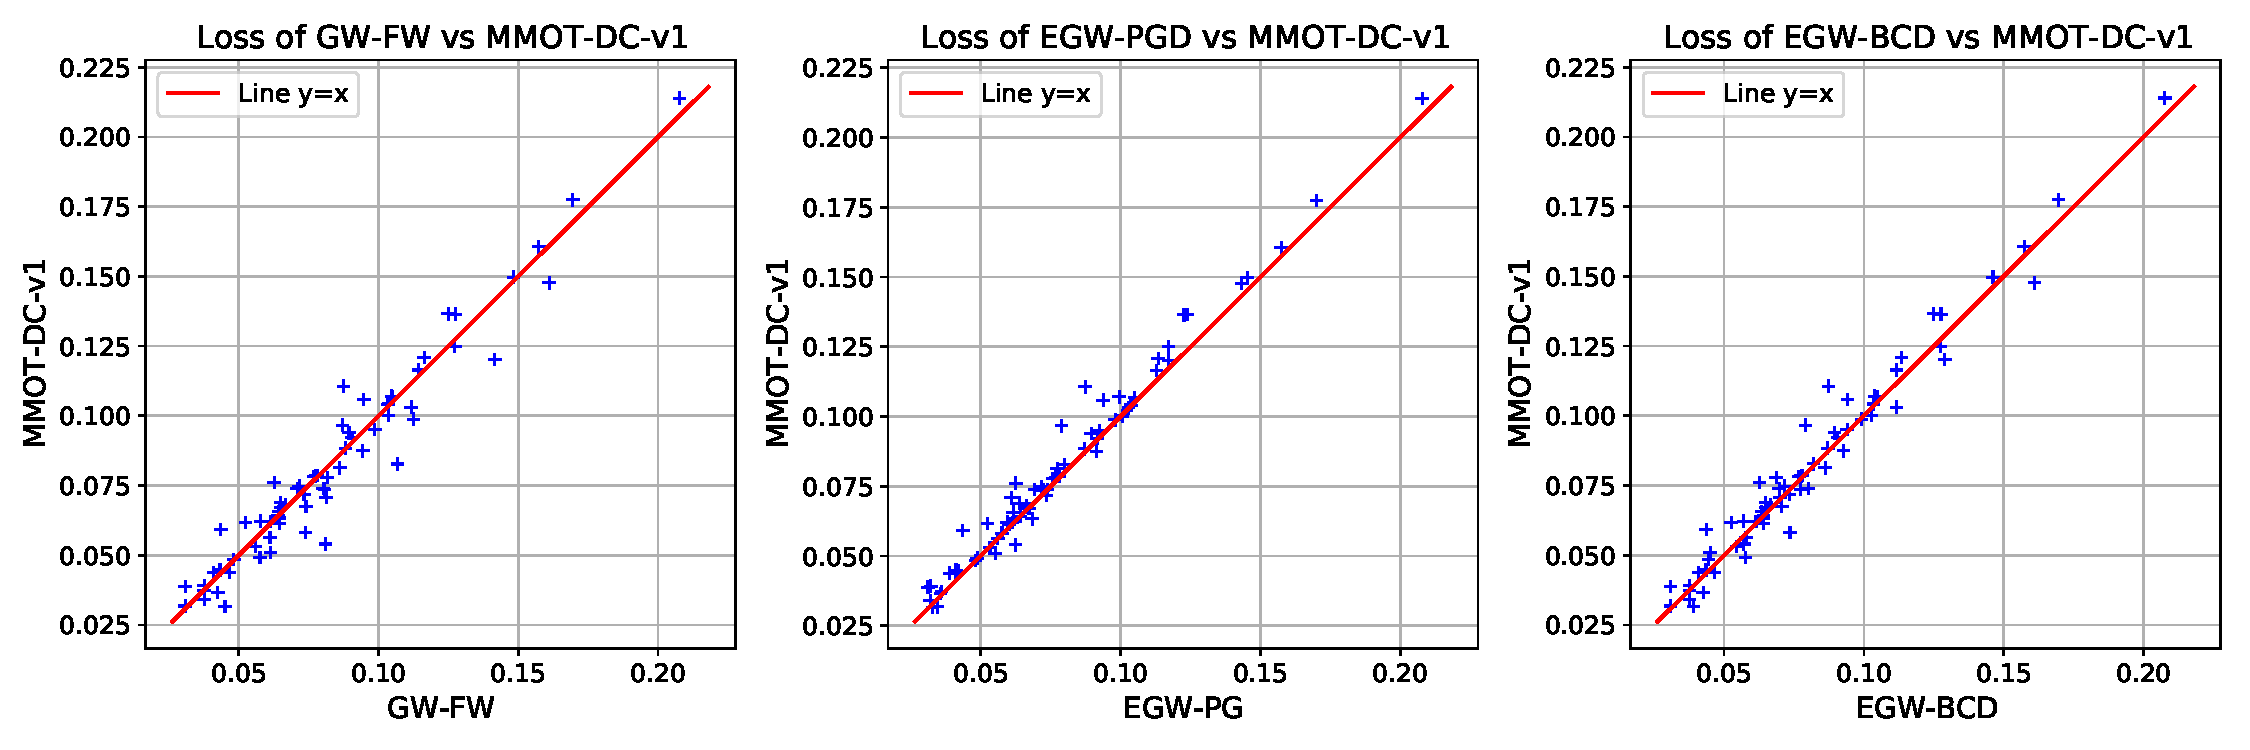
\includegraphics[width=\textwidth,height=\textheight,keepaspectratio]{./Chapitre2/fig/all_vs_MMOT-DC-v1.pdf}
  \caption{Scatter plots of MMOT-DC-v1 versus other solvers. In all three plots, the points tend to concentrate around the line $y=x$,
  which indicates the comparable performance of MMOT-DC-v1. On the other hand, the top-right plot shows the clear superiority of EGW-PGD.}
  \label{fig:coot_mmot_new}
\end{figure}

\begin{table}[H]
  \label{tab:coot_new}
  % \vskip 0.15in
  \begin{center}
    \begin{small}
      \begin{sc}
        \begin{tabular}{|c|c|}
          \hline
          MMOT-DC & MMOT-DC-v1 \\
          \hline
          0.0822 ($\pm$ 0.0364) & 0.0820 ($\pm$ 0.0361) \\
          \hline
        \end{tabular}
      \end{sc}
    \end{small}
  \end{center}
  \caption{Average and standard deviation of COOT loss of MMOT-DC and MMOT-DC-v1.
  The performance of the two algorithms is very similar.}
  % \vskip -0.1in
\end{table}

%%%%%%%%%%%%%%%%%%%%%%%%%%%%%%%%%%%%%%
\subsection{Conclusion and future work}
%%%%%%%%%%%%%%%%%%%%%%%%%%%%%%%%%%%%%%

In this section, we present a novel relaxation of the factorized MMOT problem called \textit{MMOT-DC}.
More precisely, we replace the
hard constraint on factorization constraint by a smooth regularization term. The resulting problem
not only enjoys an interpolation property between MMOT and factorized MMOT, but also is a DC problem,
which can be solved easily by the DC algorithm. We illustrate the use of MMOT-DC the via some simulated experiments and show that
it is competitive with the existing popular solvers of COOT and GW distance.
One limitation of the current DC algorithm is that, it is not scalable because
it requires storing a full-size tensor in the gradient step computation. Thus, future
work may focus on more efficiently designed algorithms, in terms of both time and memory footprint.
Moreover, incorporating additional structure on the cost tensor may also be computationally and practically beneficial.
From a theoretical viewpoint, it is also interesting to study the extension of MMOT-DC to the continuous setting,
which can potentially allow us to further understand the connection between GW distance and COOT.

% From a theoretical viewpoint, one potential application of MMOT-DC is on the study of the sample complexity of GW distance.
% More precisely, given two measure networks $\cX = (X, c_X, \mu_X)$ and $\cY = (Y, c_Y, \mu_Y)$,
% we want to quantify $| \gw(\cX, \cY) - \gw(\cX_n, \cY_n)|$. Note that, \citep{Zhang23} has also
% established the convergence rate for the case of $2$-GW distance, in which the cost function
% is the squared Euclidean distance. Our proposed approach, if works, would be able to handle any
% conditionally negative (or positive) semi-definite kernel.

% The idea is as follows: by \Cref{prop:coot_gw_equiv}, COOT and GW distance are equivalent
% \footnote{Note that one needs to properly extend \Cref{prop:coot_gw_equiv} to the continuous setting
% (of measure networks).}. So, we can replace GW by COOT, as it is less (unnecessarily) constrained.
% Next, we extend MMOT-DC to the continuous setting and show that the interpolation property
% still holds, notably MMOT-DC converges to COOT as regularization tends to the infinity.
% Thanks to the DC algo, we can linearize the MMOT-DC and obtain an entropic MMOT problem.
% This problem has two advantages. First, one can reuse the technique for entropic OT
% in \citep{Genevay19} and extend to the entropic MMOT. Second, for suitable choice of input,
% it approximates COOT.

% Note that, this is still an ongoing work as we have not yet fully resolved all
% technical difficulties. Nevertheless, we report the sketch of the proof and leave most of
% mathematical details in Appendix.

% \paragraph{Assumptions} We assume that the measure networks
% $\cX = (X, c_X, \mu_X)$ and $\cY = (Y, c_Y, \mu_Y)$. $X$ and $Y$ are compact
% subsets of $\bbR^{d_x}$ and $\bbR^{d_y}$, respectively. The probability measures
% $\mu_X$ and $\mu_Y$ are absolutely continuous with respect to the Lebesgue measures
% on $\bbR^{d_x}$ and $\bbR^{d_y}$, respectively.
% With some abuse of notation, we also use $\mu_X, \mu_Y$ to denote their density functions.

% \paragraph{Sketch of proof}
% For convenience, denote $\cU_4 = U(\mu_X, \mu_Y, \mu_X, \mu_Y)$ and $\mu = \mu_X \otimes \mu_Y$.
% We write $c = |c_X - c_Y|^2$ defined by $c(x, y, x', y') = |c_X(x, x') - c_Y(y, y') |^2$.
% Recall that, for any $\pi \in \cU_4$, we denote $\pi_{\#} = \pi_{\# 12} \otimes \pi_{\# 34}$.
% \begin{lemma}
%   For each $\pi \in \cU_4$, denote
%   $G(\pi) := \kl(\pi_{\# 12} | \mu) + \kl(\pi_{\# 34} | \mu) = \kl(\pi_{\#} | \mu^{\otimes 2})$.
%   Then $G$ is convex and differentiable. In particular, $G(\pi) = \int \nabla G(\pi) \; d \pi$,
%   for $\pi \in \cU_4$.
% \end{lemma}
% Now, we have
% \begin{align}
%   \int c \; d\gamma + \varepsilon \kl(\gamma | \gamma_{\#})
%   &\leq \int c \; d\gamma + \varepsilon \kl(\gamma | \mu^{\otimes 2})
%   - \varepsilon \Big[ G(\pi) + \int \nabla G(\pi) \; d \gamma - \int \nabla G(\pi) \; d \pi \Big] \\
%   &= \int \big[ c - \varepsilon \nabla G(\pi) \big] \; d \gamma
%   + \varepsilon \kl(\gamma | \mu^{\otimes 2}).
% \end{align}
% By taking infimum over $\cU_4$, we obtain
% \begin{align}
%   \mmotdc_{\varepsilon} \leq
%   \inf_{\gamma \in \cU_4} \int \big[ c - \varepsilon \nabla G(\pi) \big] d \gamma
%   + \varepsilon \kl(\gamma | \mu^{\otimes 2}).
% \end{align}
% Now, we define the following MMOT problem.
% \begin{definition}
%   For $\pi \in \cU_4$, define
%   \begin{align}
%     \mmot_{\varepsilon}\big( c - \varepsilon \nabla G(\pi) \big) :=
%     \inf_{\gamma \in \cU_4} \int \big[ c - \varepsilon \nabla G(\pi) \big] \; d \gamma
%       + \varepsilon \kl(\gamma | \mu^{\otimes 2}).
%   \end{align}
% \end{definition}
% There exists $\pi \in \cU_4$ such that $\mmot_{\varepsilon}\big( c - \varepsilon \nabla G(\pi) \big)$
% approximates COOT. For example, denote $\pi_{\varepsilon}$
% the solution of the entropic COOT problem $\coot_{\varepsilon}(\cX, \cY)$, we can show that
% \begin{corollary}
%   For every $\varepsilon > 0$, we have
%   $\coot_{1 / \varepsilon}(\cX, \cY) \geq
%   \mmot_{\varepsilon}\big( c - \varepsilon \nabla G(\pi_{1 / \varepsilon}) \big) \geq \mmotdc_{\varepsilon}$.
%   As a consequence,
%   $\mmot_{\varepsilon}\big( c - \varepsilon \nabla G(\pi_{1 / \varepsilon}) \big) \to \coot(\cX, \cY)$,
%   when $\varepsilon \to \infty$.
% \end{corollary}
% Now, suppose $\mmot_{\varepsilon}\big( c - \varepsilon \nabla G(\pi^*) \big)$ can approximate COOT,
% for some $\pi^* \in \cU_4$. Then, by the triangle inequality, we have
% \begin{align}
%   | \coot_(\cX, \cY) - \coot_(\cX_n, \cY_n)|
%   &\leq |\coot_(\cX, \cY) - \mmot_{\varepsilon}\big( c - \varepsilon \nabla G(\pi^*) \big)| \\
%   &+ |\mmot_{\varepsilon, n}\big( c - \varepsilon \nabla G(\pi^*) \big) - \mmot_{\varepsilon}\big( c - \varepsilon \nabla G(\pi^*) \big)| \\
%   &+ |\coot(\cX_n, \cY_n) - \mmot_{\varepsilon, n}\big( c - \varepsilon \nabla G(\pi^*) \big)|,
% \end{align}
% Now, it is enough to bound each term and obtain the final rate. However, the main difficulties
% lie on finding the appropriate choice of $\pi^*$ and on how to control
% it in the entropic MMOT problem.

% \subsection{Stability of Co-Optimal Transport}

% COOT setting: given two sample-feature spaces
% $\cX_1 = ((X_1^s, \mu_1^s), (X_1^f, \mu_1^f), \xi_1)$ and
% $\cX_2 = ((X_2^s, \mu_2^s), (X_2^f, \mu_2^f), \xi_2)$. COOT reads
% \begin{equation}
%     \coot(\cX_1, \cX_2) =
%     \inf_{\substack{\pi^s \in U() \\ \pi^f \in U()}}
%     \int |\xi_1 - \xi_2|^2 d\pi^s d\pi^f
% \end{equation}
% Consider the "semi-empirical" spaces:
% $\widehat{\cX}_i := ((\widehat{X}_i^s, \widehat{\mu}_i^s), (X_i^f, \mu_i^f), \xi_i))$, where
% we fix the dimension $f$ and only consider the empirical version of sample measures.
% Now, how does the feature coupling behave when $\widehat{\mu}^s \to \mu^s$?, i.e. when $n \to \infty$,
% quantify
% \begin{equation}
%     | \coot(\cX_1, \cX_2) -
%     \coot(\widehat{\cX}_1, \widehat{\cX}_2) |
% \end{equation}
% We can first start with finite-dimensional feature spaces (so the feature coupling is a matrix).

\vfill

\chapter[Unbalanced Co-Optimal Transport]{Unbalanced Co-Optimal Transport}
\label{chap:ucoot}

\renewcommand{\contentsname}{Contents}
\localtableofcontents*
\chaptermark{\textbf{Unbalanced Co-Optimal Transport}}

\hfill \break

\raggedbottom

% This chapter presents three contributions to the unbalanced OT-based divergences,
% namely the unbalanced OT, unbalanced Co-Optimal Transport and unbalanced Gromov-Wasserstein.

% The first contribution is an ongoing work on an alternative solver for the entropic UOT problem
% \ref{eq:discrete_ent_uot}, which has not yet been studied in the literature,
% to the best of our knowledge.
% We called this approach \textit{INexact Proximal Unbalanced optimal Transport} (INPUT),
% since it is a straightforward application of the inexact Bregman Proximal Point (BPP) algorithm
% to the UOT problem. We present the derivation of INPUT, then illustrate how
% it can overcome the limitations of the MM and Sinkhorn-based methods,
% while being orders of magnitude faster in our toy experiments. Despite the simplicity,
% its convergence analysis remains a challenging open problem and is under our active research.

This chapter summarizes the results from the paper \citep{Tran23} and addresses
the unbalanced extension of Co-Optimal transport.
Optimal transport (OT) compares probability distributions by computing a meaningful alignment
between their samples. Co-optimal transport (COOT) takes this comparison further
by inferring an alignment between features as well. While this approach leads to
better alignments and generalizes both OT and Gromov-Wasserstein distances,
we provide a theoretical result showing that it is sensitive to outliers
that are omnipresent in real-world data. This prompts us to propose unbalanced COOT
for which we provably show its robustness to noise in the compared datasets.
To the best of our knowledge, this is the first such result for OT methods in incomparable spaces.
With this result in hand, we provide empirical evidence of this robustness
for the challenging tasks of heterogeneous domain adaptation with and without
varying proportions of classes and simultaneous alignment of samples and features across
single-cell measurements.

%%%%%%%%%%%%%%%%%%%%%%%%%%%%%%%%%%%%%%%%%%%%%%
\section{Unbalanced Co-Optimal Transport}
%%%%%%%%%%%%%%%%%%%%%%%%%%%%%%%%%%%%%%%%%%%%%%

%%%%%%%%%%%%%%%%%%%%%%%%%%%%%%%%%%%%%%%%%%%%%%
\subsection{Introduction}
%%%%%%%%%%%%%%%%%%%%%%%%%%%%%%%%%%%%%%%%%%%%%%

The last decade has witnessed many successful applications of optimal
transport (OT) \citep{Monge81,Kanto42} in machine learning, namely in domain adaptation \citep{Courty16},
generative adversarial networks \citep{Arjovsky17}, classification \citep{Frogner15},
dictionary learning \citep{Rolet16}, semi-supervised learning \citep{Solomon14}. When the
supports of the probability measures lie in the same ground metric space, it is natural to use the distance defined by the metric
to induce the cost, which leads to the famous Wasserstein distance \citep{Villani03}. When they do not, one can rely on the idea of Gromov-Hausdorff distance \citep{Gromov81} and its equivalent reformulations \citep{Gromov99,Kalton99,Burago01}, and adapt them to the setting of metric measure spaces \citep{Gromov99}. This results in, for example, the Gromov-Wasserstein
(GW) distance \citep{Memoli07,Memoli11,Sturm12}, which has been widely used in many applications, namely in shape matching \citep{Memoli11},
comparing kernel matrices \citep{Peyre16}, graphs \citep{Vayer19b,Xu19,Xu19b},
computational biology \citep{Demetci22}, heterogeneous domain adaptation \citep{Yan18},
correspondence alignment \citep{Solomon16}, machine translation \citep{Melis18}.

By construction, the GW distance can only provide the sample alignment that best preserves the intrinsic geometry of the distributions and, as such, compares square pairwise relationship matrices. The CO-Optimal transport (COOT) \citep{Redko20,Chowdhury21b} goes beyond these limits by simultaneously learning two independent (feature and sample) correspondences, and thus provides greater flexibility over the GW distance in terms of usage and interpretability. First, it allows us to measure similarity between arbitrary-size matrices. An interesting use case is, for instance, on tabular data, which are usually expressed as a matrix whose rows represent samples and columns represent features. For the GW distance,
the similarity or distance matrix (or any square matrix derived from the data)
must be calculated in advance and the effect of the individual variables is lost during this computation. On the other hand, COOT can bypass this step as it can use either the tabular data directly or the similarity matrices as inputs. Second, COOT provides both sample and feature correspondences. These feature correspondences are also interpretable and allow to recover relations between the features of two different datasets even when they do not lie in the same space.

Similar to classical OT, COOT enforces hard constraints on the marginal distributions
both between samples and features. These constraints lead to two main limitations:
(1) imbalanced datasets where samples or features are re-weighted
cannot be accurately compared; (2) mass transportation \emph{must} be exhaustive:
outliers, if any, must be matched regardless of the cost they induce.
To circumvent these limitations, we propose to relax the mass preservation constraints
in the COOT distance and study a broadly applicable and general OT framework
that includes several well-studied cases presented in \Cref{t:ucoot_comparisons}.

\paragraph{Related work.}
To relax the OT marginal constraints, a straightforward solution is to control
the difference between the marginal distributions of the transportation plan
and the data by some discrepancy measure, e.g., Kullback-Leibler divergence.
In classical OT, this gives rise to the unbalanced OT (UOT),
which was first proposed by \citet{Benamou03}.
The theoretical and numerical aspects of this extension
have been studied extensively \citep{Liero18,Chizat18b,Chizat18a,Khiem20}
and are gaining increasing attention in the machine
learning community, with wide-range applications, namely in
domain adaptation \citep{Fatras21}, generative adversarial networks
\citep{Balaji20, Yang19}, dynamic tracking \citep{Lee19}, crowd counting \citep{Ma21},
neuroscience \citep{janati2019group, bazeille2019} or
modeling cell developmental trajectories \citep{Schiebinger19}.

Unbalanced OT and its variants are usually sought for
their known robustness to outliers \citep{Mukherjee21,Balaji20,Fatras21}.
This appealing property goes beyond classical OT. For instance,
to compare signed and non-negative measures in incomparable spaces,
unbalanced OT \citep{Liero18} can be blended with the
$L_p$-transportation distance \citep{Sturm06}, which leads to the
Sturm-Entropic-Transport distance \citep{Ponti20}, or with the GW distance,
which gives rise to the unbalanced GW (UGW) distance \citep{Sejourne20}.
Also motivated by the unbalanced OT, \citet{Zhang21} proposed a relaxation of the
bidirectional Gromov-Monge distance called unbalanced bidirectional Gromov-Monge divergence.
\begin{table}[t]
  \small
	\centering
  \begin{tabular}{l *4c}
    \toprule
    & Across spaces & Sample alignment & Feature alignment & \makecell{Robust to outliers} \\
    \midrule
    OT & \nomark & \yesmark & \nomark & \nomark \citep{Fatras21} \\
    UOT & \nomark & \yesmark & \nomark & \yesmark \citep{Fatras21} \\
    GW & \yesmark & \yesmark & \nomark & \nomark (Prop. \ref{prop:coot_not_robust}) \\
    UGW & \yesmark & \yesmark & \nomark & \yesmark (Thm. \ref{thm:ucoot_robust}) \\
    COOT & \yesmark & \yesmark & \yesmark & \nomark (Prop. \ref{prop:coot_not_robust}) \\
    UCOOT & \yesmark & \yesmark & \yesmark & \yesmark (Thm. \ref{thm:ucoot_robust}) \\
    \bottomrule
    \hline
  \end{tabular}
  \caption{Properties of different OT formulations generalized by UCOOT.
  The proposed UCOOT is not only able to learn informative feature alignments,
  but also robust to outliers.
  \label{t:ucoot_comparisons}}
\end{table}

\paragraph{Contributions.} In this work, we introduce an unbalanced extension of COOT
called ``Unbalanced CO-Optimal transport'' (UCOOT). UCOOT -- defined for both discrete and
continuous data -- is a general framework that encompasses all the OT variants displayed
in \Cref{t:ucoot_comparisons}. Our main contribution is to show that UCOOT is provably robust
to both samples and features outliers, while its balanced counterpart can be made
arbitrarily large with strong enough perturbations. To the best of our knowledge,
this is the first time such a general robustness result is established for OT across different spaces.
Our theoretical findings are showcased in unsupervised heterogeneous domain adaptation
and single-cell multi-omic data alignment, demonstrating a very competitive performance.

\paragraph{Notations.} For any integer $n \geq 1$, we write $[n] := \{1,...,n\}$.
Given a Polish space $X$, we denote $\cM^+(X)$ the set of nonnegative and finite Borel
measures over $X$. For any $\mu \in \cM^+(X)$, we denote
its mass by $m(\mu) := \mu(X)$.
Unless specified otherwise, we always consider fully supported measures,
i.e. $\text{supp}(\mu) = X$, for any measure $\mu \in \cM^+(X)$.
The product measure of two measures $\mu$ and $\nu$ is defined as:
$d (\mu \otimes \nu)(x,y) := d\mu(x) d\nu(y)$.
Given $\pi \in \cM^{+}(X \times Y)$, we denote
$(\pi_{\#1}, \pi_{\#2})$ its marginal distributions i.e. $d\pi_{\#1} = \int_{Y} d\pi$ and
$d\pi_{\#2} = \int_{X} d\pi$.
For $\mu, \nu \in \cM^+(X)$, the Kullback-Leibler divergence is defined by
$\kl(\mu|\nu) := \int \frac{d \mu}{ d \nu} \log \frac{d \mu}{ d \nu} \mathrm d\nu
- \int \mathrm d\mu + \int \mathrm d\nu$ if $\mu \ll \nu$ and set to $+\infty$ otherwise.
Finally, the indicator divergence $\iota_{=}(\mu | \nu)$ is equal to 0 if $\mu = \nu$
and $+\infty$ otherwise.

%%%%%%%%%%%%%%%%%%%%%%%%%%%%%%%%%%%%%%%%%%%%%%%%%%

%%%%%%%%%%%%%%%%%%%%%%%%%%%%%%%%%%%%%%%%%%%%%%%
\subsection{From COOT to Unbalanced Co-Optimal Transport} \label{sec:ucoot}
The ultimate goal behind the CO-Optimal Transport (COOT)
framework is the simultaneous alignment of samples \emph{and} features to allow for
comparisons across spaces of different dimensions. In this section, we discuss
OT formulations including OT, UOT, GW, UGW and COOT, then introduce the proposed UCOOT
and show how the aforementioned distances fall into our framework.

% \iffalse After some examples, we present our main theoretical contribution:the robustness to sample and feature outliers. \fi

\paragraph{From sample alignment to sample-feature alignment.}
Let $(X_1^s, \mu_1^s)$ and $(X_2^s, \mu_2^s)$ be a pair of compact measure spaces such that
$X_1^s$ and $X_2^s$ belong to some common metric space $(\cE, d)$.
Classical (unbalanced) optimal transport infers one alignment (or joint distribution)
$\pi^s \in \cM^+(X_1^{s} \times X_2^s)$ with marginals $(\pi^{s}_{\#1}, \pi^{s}_{\#2})$
close to $(\mu_1^s, \mu_2^s)$ according to some appropriate divergence $D$ such that
the cost $\int c(x_1, x_2) \; \mathrm d\pi^{s}(x_1, x_2) + D(\pi^{s}_{\#1} | \mu_1^s)
+ D(\pi^{s}_{\#2} | \mu_2^s)$ is minimal. For instance, in balanced (resp. unbalanced) OT,
$D$ corresponds to the indicator divergence (resp. KL divergence or TV).
To define a generalized OT beyond one single alignment, we must first introduce
a new pair of measure spaces $(X_1^{f}, \mu_1^f)$ and $(X_2^{f}, \mu_2^f)$.
Intuitively,  the two transport plans that must be inferred: $\pi^s$ across \emph{samples}
and $\pi^f$ across \emph{features}, must minimize a cost of the form
$\iint c((x_1^s, x_1^f), (x_2^s, x_2^f)) \; \mathrm d\pi^s(x_1^s, x_2^s)\; \mathrm d \pi^f(x_1^f, x_2^f)$
where $c((x_1^s, x_1^f), (x_2^s, x_2^f))$ is the \emph{joint} cost of aligning
the sample-feature pairs $(x_1^s, x_1^f)$ and $(x_2^s, x_2^f)$.

However, unlike OT,
there is no underlying ambient metric space in which comparisons between these pairs
are straightforward. Thus, we consider a simplified cost of the form:
$c((x_1^s, x_1^f), (x_2^s, x_2^f)) = |\xi_1(x_1^s, x_1^f) - \xi_2(x_2^s, x_2^f)|^p$, for $p \geq 1$
and some scalar functions $\xi_1, \xi_2$ that define the sample-feature interactions.
A similar definition was adopted by \citet{Chowdhury21b} to extend COOT to the continuous setting
in the context of hypergraphs. Formally, our general formulation takes
pairs of \emph{sample-feature spaces} defined as follows.

\begin{definition}[Sample-feature space]
Let $(X^s, \mu^s)$ and $(X^f, \mu^f)$ be compact Polish measure spaces, where $\mu^f \in \cM^+(X^f)$
and $\mu^s \in \cM^+(X^s)$. Let $\xi$ be a scalar integrable function in
$L^p(X^s \times X^f, \mu^s \otimes \mu^f)$. We call the triplet
$\cX = ((X^s, \mu^s), (X^f, \mu^f), \xi)$ a sample-feature space and $\xi$ is called an interaction.
\end{definition}
%
%%%%%%%%%%%%%%%%%%%%%%%%%%%%%%%%%%%%%%%%%%%%%%%%
\begin{definition}[Generalized COOT]
\label{def:ucoot}
Given two divergences $D_1$ and $D_2$, we define the generalized COOT of order $p$
between $\cX_1 = ((X_1^s, \mu_1^s), (X_1^f, \mu_1^f), \xi_1)$ and
$\cX_2 = ((X_2^s, \mu_2^s), (X_2^f, \mu_2^f), \xi_2)$ by:
\begin{equation}
\label{eq:ucoot}
  \begin{split}
  \inf_{\substack{\pi^s \in \cM^+(X_1^s \times X_2^s) \\
  \pi^f \in \cM^+(X_1^f \times X_2^f) \\ m(\pi^s) = m(\pi^f)}}
  &\underbrace{\iint |\xi_1(x_1^s, x_1^f) - \xi_2(x_2^s, x_2^f)|^p
  \; \mathrm d\pi^s \; \mathrm d \pi^f}_{\text{transport cost of sample-feature pairs}}
  + \underbrace{\sum_{k=1}^2\rho_k D_k(\pi^s_{\#k} \otimes \pi^f_{\#k} |
  \mu^s_k \otimes \mu^f_k)}_{\text{mass destruction / creation penalty}},
  \end{split}
\end{equation}
for $\rho_1, \rho_2 >0$ and $p \geq 1$.
\end{definition}
As the multiplicative nature between $\pi^s$ and $\pi^f$ leads to an invariance by the scaling map
$\alpha \mapsto (\alpha \pi^s, \frac{1}{\alpha} \pi^f)$, for $\alpha > 0$,
we further impose the equal mass constraint $m(\pi^s) = m(\pi^f)$.

It is worth mentioning that Formulation \eqref{eq:ucoot} is not the only way to
relax the marginal constraints. For example, instead of
$D_k(\pi^s_{\#k} \otimes \pi^f_{\#k} | \mu^s_k \otimes \mu^f_k)$,
one can consider $D_k(\pi^s_{\#k} | \mu^s_k) + D_k( \pi^f_{\#k} | \mu^f_k)$,
or $D_s(\pi^s_{\#1} \otimes \pi^s_{\#2} | \mu^s_1 \otimes \mu^s_2)$,
for some divergence $D_s$. However, amongst these choices,
ours is the only one which can be recast as a variation of the unbalanced OT problem.
This allows us to leverage the known techniques in unbalanced OT to justify
the theoritical and practical properties, namely \Cref{prop:existence}
and \Cref{thm:ucoot_robust} below.

Note that the problem above is very general and can, with some additional
constraints, recover exact OT, UOT, GW, UGW, COOT (see \Cref{t:examples}).
In particular, if the measures $(\mu^s_1, \mu^s_2)$ and $(\mu^f_1, \mu^f_2)$
are probability measures, then setting $D_1 = D_2 = \iota_=$ leads to the
COOT problem first introduced in the discrete case in \citep{Redko20} and
recently generalized to the continuous setting in \citep{Chowdhury21b}
\footnote{Note that, \citet{Chowdhury21b} consider \textbf{bounded measurable} function
on the Polish measure space, whereas we work with \textbf{integrable} function
on the \textbf{compact} Polish measure space.}
In this work, we relax the hard constraints and consider a more flexible formulation
with the KL divergence:
\begin{definition}[UCOOT]
   We define Unbalanced COOT (UCOOT) as in \Cref{eq:ucoot} with $D_1 = D_2 = \kl$.
   We write $\ucoot_{\rho}(\cX_1, \cX_2)$ to indicate the UCOOT between
   two sample-feature spaces $\cX_1$ and $\cX_2$, for a given
   pair of hyperparameters $\rho = (\rho_1, \rho_2)$.
\end{definition}
While various properties of the divergences $D_k$ have been extensively studied
in the context of unbalanced OT by several authors \citep{Chizat17,Frogner15},
the concept of sample-feature interaction requires more clarification.
Let us consider some simple examples.
In the discrete case, we consider $n$ observations of $d$ features
represented by matrix $A \in \bbR^{n \times d}$. In this case, the space $X^s$ (resp. $X^f$)
is not explicitly known but can be characterized by the finite set $[n]$ (resp. $[d]$),
up to an isomorphism. Assuming that all samples (resp. features) are equally important,
the discrete empirical measures can be given by uniform weights $\mu^s = \frac{1_{n}}{n}$
(resp. $\mu^f = \frac{1_{d}}{d}$). The most natural sample-feature interaction $\xi$ is simply
the index function $\xi(i, j) = A_{ij}$. In the continuous case,
we assume that data stream from a continuous random variable $a \sim \mu_s \in \cP(\bbR^d)$
for which an interaction function can be $\xi(a, j) = a_j$.
\begin{table}[t]
  \centering
  \small
  \begin{tabular}{l *4c}
      \toprule
          & Shape of inputs & Coupling constraint & Scalar function & Divergence \\
      \midrule
      OT   & $d_1 = d_2$              & $\pi^f = I_{d_1} = I_{d_2}$ & $\xi(i, j) = A_{ij}$                        & $\iota_=$ \\
      GW   & $n_1 = d_1$, $n_2 = d_2$ & $\pi^f = \pi^s$             & $\xi(i, j) = \text{dist}( A_{i.}, A_{j.} )$ & $\iota_=$ \\
      COOT & --                       & --                          & $\xi(i, j) = A_{ij}$                        & $\iota_=$ \\
      semi-d. COOT & --               & --                          & $\xi(a, j) = a_j$                           & $\iota_=$ \\
      UCOOT & --                      & --                          & $\xi(i, j) = A_{ij}$                        & KL \\
        \bottomrule
        \hline
        \end{tabular}
        \caption{Conditions under which different OT formulations fall within
        the generalized framework of \Cref{def:ucoot}.
        ``semi-d'' refers to ``semi-discrete'' setting, where
        $\mu_s$ is a continuous probability and $\mu_d = 1_d/d$.
        Here, $I_d$ is the identity matrix in $\bbR^d$.
  \label{t:examples}}
\end{table}
\begin{proposition} \label{prop:existence}
For any $D_1$, $D_2 \in \{ \iota_{=}, \kl \}$, Problem \eqref{def:ucoot} (in Equation \eqref{eq:ucoot})
admits a minimizer.
\end{proposition}

\begin{remark}
The existence of minimizer shown in \Cref{prop:existence}
can be extended to a larger family of Csiszár divergences \citep{Csiszar63}.
A general proof is given in the Appendix.
\end{remark}

\paragraph{Relation between UCOOT and COOT.} When $ \mu^s_k$ and $\mu^f_k$ are probability measures,
for $k=1,2$, then $\ucoot_{\rho}(\cX_1, \cX_2) \leq \coot(\cX_1, \cX_2)$,
for any $\rho_1, \rho_2 > 0$.
Moreover, $\ucoot_{\rho}(\cX_1, \cX_2) = 0$ if and only if $\coot(\cX_1, \cX_2) = 0$.
In particular, suppose that $\cX_1$ and $\cX_2$ are two finite sample-feature spaces
such that $(X^s_1, X^s_2)$ and $(X^f_1, X^f_2)$ have the same cardinality and
are equipped with the uniform measures $\mu_1^s = \mu_2^s$, $\mu_1^f = \mu_2^f$.
Then $\ucoot_{\rho}(\cX_1, \cX_2) = 0$ if and only if
there exist perfect alignments between rows (samples) and between
columns (features) of the interaction matrices $\xi_1$ and $\xi_2$.

\paragraph{Relation between UCOOT and its solution.}
UCOOT is a quadratic function of its minimizer, thanks to the property of the
KL divergence. More precisely, if $(\pi_*^s, \pi_*^f)$ is the equal-mass solution,
then by using the proof technique of Lemma 4 in \citep{Khiem20}, one can show that
\begin{align}
  \label{eq:ucoot_minimizer_minimum}
  \ucoot_{\rho}(\cX_1, \cX_2) =
  \sum_{k=1, 2} \rho_k \; m(\mu_k^s) \; m(\mu_k^f) - (\rho_1  + \rho_2) \; m(\pi^s_*)^2.
\end{align}

\subsection{Robustness of Unbalanced Co-Optimal Transport} \label{sec:robustness}
When discussing the concept of robustness, outliers are often considered as samples
not following the underlying distribution of the data. In our general context of
sample-feature alignments, we consider a \emph{pair} $(x^s, x^f) \in X^s \times X^f$
to be an outlier if the magnitude of $|\xi(x^s, x^f)|$ is abnormally larger than
other interactions between $X^s$ and $X^f$. As a result, such outliers lead to
abnormally large transportation costs $|\xi_1 - \xi_2|$. To study the robustness of COOT and UCOOT,
we consider an outlier scenario where the marginal data distributions are contaminated
by some additive noise distribution.
\begin{assumption}
\label{assump:robust}
Consider two sample-feature spaces $\cX_1$ and $\cX_2$.
Let $\varepsilon^s$ (resp. $\varepsilon^f$) be a probability measure with
compact support $O^s$ (resp. $O^f$). For $a \in \{s, f\}$,
define the noisy distribution $\widetilde{\mu}^a = \alpha_a \mu^a + (1-\alpha_a) \varepsilon^a$,
where $\alpha_a \in [0,1]$. We assume that $\xi_1$ is defined on
$(X^s_1 \cup O^s) \times (X^f_1 \cup O^f)$ and
that $\xi_1, \xi_2$ are continuous on their supports.
We denote the contaminated sample-feature space by
$\widetilde{\cX_1} = ((X^s_1 \cup O^s, \widetilde{\mu}^s_1), (X^f_1 \cup O^f, \widetilde{\mu}^f_1), \xi_1)$.
Finally, we define some useful minimal and maximal costs:
  \begin{equation}
    \begin{cases}
  \Delta_{0} := \min\limits_{
  \substack{
       x_1^s \in O^s, x_1^f \in O^f  \\
       x_2^s \in X_2^s, x_2^f \in X_2^f
  }}\quad |\xi_1(x_1^s, x_1^f) - \xi_2(x_2^s, x_2^f)|^p \\
  \Delta_{\infty} := \max\limits_{
  \substack{
  x_1^s \in X_1^s \cup O^s, x_1^f \in X_1^f \cup O^f \\
  x_2^s \in X_2^s, x_2^f \in X_2^f
  }} \quad|\xi_1(x_1^s, x_1^f) - \xi_2(x_2^s, x_2^f)|^p \enspace.
  \end{cases}
  \end{equation}
Here, $\Delta_{0}$ accounts for the minimal deviation of the cost between
the outliers and target support, while $\Delta_{\infty}$ is the maximal deviation
between the contaminated source and the target.
\end{assumption}
The exact marginal constraints of COOT enforce conservation of mass.
Thus, outliers \emph{must} be transported no matter how large their transportation costs are.
This intuition is captured by the following result.
%%%%%%%%%%%%%%%%%%%%%%%%
\begin{proposition}[COOT is sensitive to outliers]
Consider $\widetilde{\cX_1}, \cX_2$ as defined in \Cref{assump:robust}.
Then
\label{prop:coot_not_robust}
\begin{equation}
    \coot(\widetilde{\cX_1}, \cX_2) \geq (1 - \alpha_s)(1-\alpha_f)\Delta_0.
\end{equation}
\end{proposition}
%%%%%%%%%%%%%%%%%%%%%%%%
Whenever the outlier proportion $(1-\alpha_s)(1-\alpha_f)$ is positive,
COOT increases with the distance between the supports of the outliers and those of the clean data.
Thus, the right hand side of \Cref{prop:coot_not_robust} can be made arbitrarily
large by taking outliers far from the supports of the clean data.

We can now state our main theoretical contribution.
Relaxing the marginal constraints leads to a loss that saturates
as outliers get further from the data:
\begin{theorem}[UCOOT is robust to outliers]
\label{thm:ucoot_robust}
Consider two sample-feature spaces $\widetilde{\cX_1}, \cX_2$ as defined
in \Cref{assump:robust}. Let $\delta := 2(\rho_1 + \rho_2)(1 - \alpha_s\alpha_f)$
and $K = M + \frac{1}{M}\ucoot(\cX_1, \cX_2) +\delta$,
where $M= m(\pi^s) = m(\pi^f)$ is the transported mass between clean data. Then:
\begin{align} %\label{eq:ucoot-robust}
  \ucoot(\widetilde{\cX_1}, \cX_2)
  &\leq \alpha_s \alpha_f \ucoot(\cX_1, \cX_2)
  + \delta M \left[ 1 - \exp \left( {- \frac{\Delta_{\infty}(1+M) + K}{\delta M}} \right) \right].
\end{align}
\end{theorem}
%%%%%%%%%%%%%%%%%%%%%%%%%%%%%%%%%%%%%%%%%
The proof of \Cref{thm:ucoot_robust} is provided in the Appendix and
inspired from \citep{Fatras21}, but in a much more general setting:
(1) it covers both sample and feature outliers and
(2) considers a noise distribution instead of a Dirac.
Note that the bound in \Cref{prop:coot_not_robust}
indicates that outliers can make COOT arbitrary large,
while UCOOT is upper bounded and discards the mass of outliers with high transportation cost.

\setlength{\columnsep}{10pt}%
\setlength{\intextsep}{0pt}
\begin{wrapfigure}[10]{r}{0.4\textwidth}
  \centering
  \vspace{-10pt}
  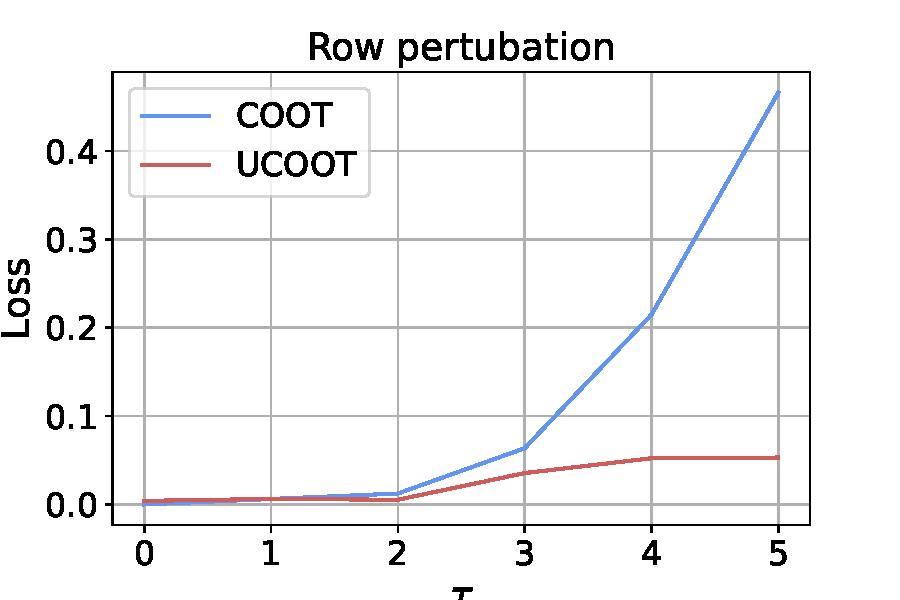
\includegraphics[width=\linewidth]{./Chapitre3/fig/robustness_2.pdf}
  \caption{Sensitivity of COOT and UCOOT under the presence of outliers.
  \label{fig:robust}}
% \end{figure}
\end{wrapfigure}
This is well illustrated in \Cref{fig:robust},
where we simulate outliers by adding a perturbation to a row of the interaction matrix.
More precisely, we first generate a matrix $A \in \mathbb R^{20 \times 15}$ by
$A_{ij} = \cos(\frac{i}{20} \pi) + \cos(\frac{j}{15} \pi)$.
Then, we replace its last row by $\tau 1_{15}$, for $\tau \geq 0$.
\Cref{fig:robust} depicts COOT and UCOOT between $A$
and its modified version as a function of $\tau$. The higher the value of $\tau$,
the more likely that the last row contains the interaction of outliers.
Consequently, as $\tau$ increases, so does COOT but at a much higher pace,
whereas UCOOT remains stable.

It should be noted that, with minimal adaptation, \Cref{thm:ucoot_robust}
also holds for the unbalanced GW (UGW) distance.
This provides a theoretical explanation of the empirical observation in \citep{Sejourne20}
that unlike GW, the UGW distance is also robust to outliers.

%%%%%%%%%%%%%%%%%%%%%%%%%%%%%%%%%%%%%%%%%%%%%%%%
\subsection{Optimization algorithm and complexity} \label{subsec_app:algo}
%%%%%%%%%%%%%%%%%%%%%%%%%%%%%%%%%%%%%%%%%%%%%%%%
Solving COOT-type problems, in general, is not trivial. As highlighted in \citep{Redko20},
the balanced case corresponds to a convex relaxation of the bilinear assignment problem,
which seeks the pair of permutations minimizing the transport cost.
Here we argue that relaxing the marginal constraints makes the problem easier
in two different aspects: (1) the obtained problem is easier to solve
through a sequence of GPU friendly iterations; (2) regularization leads to lower alignment costs
and thus better local minima. In this section, we first describe how to compute UCOOT in practice.

\paragraph{Optimization strategy}
We consider two tabular datasets $A \in \bbR^{n_1 \times d_1}$ and $B \in \bbR^{n_2 \times d_2}$.
Let $u_k$ be the uniform histogram over sample-feature pairs:
$u_k := \frac{1}{n_kd_k}1_{n_k} \otimes 1_{d_k}$, for $k=1, 2$.
For the sake of simplicity, we assume uniform weights over both samples and features.
Computing UCOOT can be done using block-coordinate descent (BCD) both with
and without entropy regularization. More precisely, given a hyperparameter $\varepsilon \geq 0$,
discrete UCOOT can be written as:
\begin{equation}
\begin{split}
    \label{eq:ucoot-discrete-2}
  &\min_{\substack{\pi^s, \pi^f \\
  \iffalse \in \bbR_+^{n_1, n_2} \\ \pi^f \in \bbR_+^{d_1, d_2} \\ \fi m(\pi^s) = m(\pi^f)}}
  \sum_{i, j, k, l} (A_{ik} - B_{jl})^2\pi^s_{ij}\pi^f_{kl} +
  \rho_1 \kl(\pi^s 1_{n_1} \otimes \pi^f 1_{d_1} | u_1 )  \\
  &+ \rho_2 \kl({\pi^s}^\top 1_{n_2} \otimes {\pi^f}^{\top} 1_{d_2} | u_2) +
  \varepsilon \text{KL}( \pi^s \otimes \pi^f | \mu^s_1 \otimes \mu_2^s \otimes \mu_1^f \otimes \mu_2^f).
\end{split}
\end{equation}

\begin{algorithm}[t]
    \caption{BCD algorithm to solve UCOOT \label{alg:bcd}}
    \begin{algorithmic}
      \STATE {\bfseries Input:} $A \in \bbR^{n_1, d_1}, B \in \bbR^{n_2, d_2}$, $\rho_1, \rho_2, \varepsilon$
      \STATE Initialize $\pi^s$ and $\pi^f$
      \REPEAT
      \STATE Update $\pi^s$ using Sinkhorn or MM
      \STATE Rescale $\pi^s = \sqrt{\frac{m(\pi^f)}{m(\pi^s)}} \pi^s$
      \STATE Update $\pi^s$ using Sinkhorn or MM
      \STATE Rescale $\pi^f = \sqrt{\frac{m(\pi^s)}{m(\pi^f)}} \pi^f$
      \UNTIL{convergence}
	\end{algorithmic}
\end{algorithm}
The only difference between $\varepsilon = 0$ and $\varepsilon > 0$
lies in the inner-loop algorithm used to update one of transport plans $(\pi^s, \pi^f)$
while the other one remains fixed.
For $\varepsilon=0$, we use the Majorization-Minimization (MM) algorithm \citep{Chapel21},
which leads to a multiplicative update on the transport plan.
For $\varepsilon > 0$, updating each transport plan boils down to an entropic UOT problem,
which can be solved efficiently using the unbalanced variant of Sinkhorn's algorithm \citep{Chizat18a}.
The main benefit of entropy regularization is to reduce the number of variables
from $(n_1 \times n_2) + (d_1 \times d_2)$ to $n_1 + n_2 + d_1 + d_2$.
Moreover, by taking $\varepsilon$ sufficiently small, we can recover solutions
close to those in the non-entropic case. We formalize this claim in the following result.
%%%%%%%%%%%%%%%%%%%%%%%%%%%%%%%%%%%%%%%%%%
\begin{proposition}
  \label{prop:convergence_minimiser_unbalanced}
  Let $(\pi_{\varepsilon}^s, \pi_{\varepsilon}^f)$ be an equal-mass solution of the problem
  $\ucoot_{\rho, \varepsilon}(\cX_1, \cX_2)$. Denote $\mu^s = \mu_1^s \otimes \mu_2^s$
  and $\mu^f = \mu_1^f \otimes \mu_2^f$.
  \begin{enumerate}
    \item When $\varepsilon \to \infty$, we have $\pi_{\varepsilon}^s \rightharpoonup
    \sqrt{\frac{m(\mu^f)}{m(\mu^s)}} \mu^s$
    and $\pi_{\varepsilon}^f \rightharpoonup \sqrt{\frac{m(\mu^s)}{m(\mu^f)}} \mu^f$.

    \item When $\varepsilon \to 0$, we have
    \begin{enumerate}
      \item $\ucoot_{\rho, \varepsilon}(\cX_1, \cX_2) \to \ucoot_{\rho}(\cX_1, \cX_2)$ and
      $m(\pi_{\varepsilon}^s) \to m(\pi_*^s)$, for any equal-mass solution
      $(\pi_*^s, \pi_*^f)$ of the unregularized problem.

      \item Any cluster point $(\widehat{\pi}^s, \widehat{\pi}^f)$ of the sequence
      $(\pi_{\varepsilon}^s, \pi_{\varepsilon}^f)_{\varepsilon}$ is an equal-mass
      solution of the unregularized problem. Furthermore,
      \begin{equation}
        \kl(\widehat{\pi}^s \otimes \widehat{\pi}^f | \mu^s \otimes \mu^f) =
        \min_{(\pi^s, \pi^f)} \kl(\pi^s \otimes \pi^f \vert \mu^s \otimes \mu^f),
      \end{equation}
      where the infimum is taken over all solutions of the unregularized problem.
    \end{enumerate}
  \end{enumerate}
\end{proposition}

%%%%%%%%%%%%%%%%%%%%%%%%%%%%%%%%%%%%%%%%%%%%%%%%
\subsection{Experiments} \label{sec:experiments}
\subsubsection{Illustration and interpretation on MNIST images}

\begin{figure}[t]
  \centering
  \includegraphics[trim={0.5cm 4.5cm 1.5cm 2.4cm}, clip, width=\linewidth]{./Chapitre3/fig/mnist-ucoot-rebuttal.pdf}
  \caption{Example illustrating the feature alignment $\pi_f$ learned by UCOOT
  and its robustness to outliers.
  \textbf{(a)} Visualization of 4 random samples from both datasets.
  The added Gaussian noise only affects the first 10 columns of the images
  and is different across images.
  \textbf{(b)} The barycentric mapping (see Appendix for details)
  defined by UCOOT learns the transformation defined by $\varphi_\sigma$
  while disregarding non-informative features.
  \textbf{(c)} Alignments across samples from $X$ and $Y$.
  We contaminated the target $Y$ with 50 sample outliers
  (images with uniform entries in $[0,1]$).
  A very small amount of noise is sufficient to derail COOT.
  Unlike COOT, UCOOT does not transport any outlier sample.
  Accuracy is computed as the percentage of mass within the block-diagonal structure.
  \label{f:mnist-example}}
\end{figure}
We illustrate the robustness of UCOOT and its ability to learn meaningful feature alignments
under the presence of both sample and feature outliers in the MNIST dataset.
We introduce the feature outliers by applying a handcrafted transformation $\varphi_\sigma$
that performs a zero-padding (shift), a 45\textdegree\ rotation,
a resize to (28, 34) and adds Gaussian noise $\cN(0, \sigma^2)$ entries
to the first 10 columns of the image.

\Cref{f:mnist-example} (a) shows some examples of original and transformed images.
We randomly sample 100 images per class (1000 total) from $X = \text{MNIST}$ and
$Y = \varphi_{\sigma}(\text{MNIST})$. Regarding the sample outliers,
we add 50 random images with uniform entries in [0, 1] to the target data $Y$.
We then compute the optimal COOT and UCOOT alignments shown in
\Cref{f:mnist-example} (b) and (c).
The flexibility of UCOOT with respect to mass transportation allows it to completely disregard:
(1) noisy and uninformative pixels (features),
which are all given the same weight as depicted by (b);
(2) all the sample outliers of which none are transported as shown
by the last blank column of the alignment (c).
Moreover, notice how the color-coded input image is transformed according to
the transformation $\varphi_{\sigma}$ despite the fact that
no spatial information is provided in the OT problem. On the other hand,
a very small perturbation ($\sigma = 0.01)$ is enough for the sample alignment
given by COOT to lose its block-diagonal dominant structure (class information is lost),
while the UCOOT alignment remains unscathed.

\setlength{\intextsep}{0pt}
\begin{wrapfigure}[10]{r}{0.4\textwidth}
    \centering
    \vspace{-12pt}
    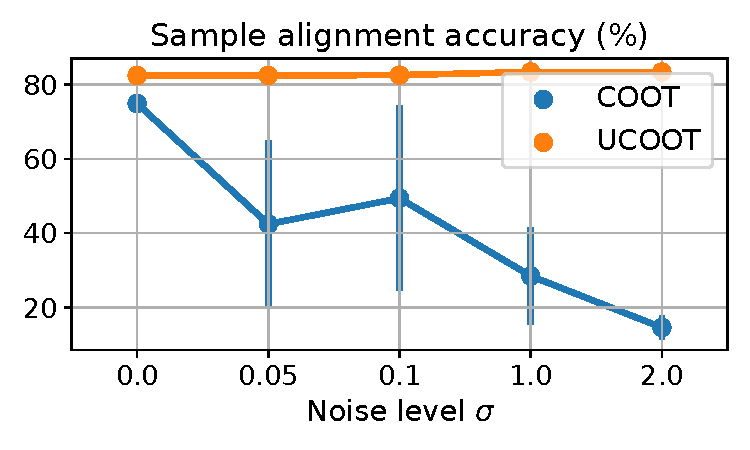
\includegraphics[width=\linewidth]{./Chapitre3/fig/mnist-sigma.pdf}
    \vspace*{-9mm}
    \caption{Robustness of UCOOT vs. COOT on MNIST example, at different noise levels.
    \label{f:mnist-sigma}}
\end{wrapfigure}
One may wonder whether the performance of UCOOT would still hold for different values of $\sigma$.
\Cref{f:mnist-sigma} answers this question positively.
For $\sigma > 0$, we compute the average accuracy
(defined by the percentage of mass within the block-diagonal structure) over 20 different runs.
The performance of COOT not only degrades with noisier outliers but is also unstable.
By contrast, the accuracy of UCOOT remains almost constant regardless of the level of noise.

\subsubsection{Heterogeneous Domain Adaptation}

%Domain adaptation (DA) refers to the problem in which a classifier
%learned on one domain (called \textit{source}) can generalise well to the other one (called \textit{target}).
We now investigate the application of discrete UCOOT in semi-supervised and unsupervised
Heterogeneous Domain Adaptation (HDA). It is a particularly difficult problem where
one aims to predict classes on unlabeled data using labeled data lying in a different space.
OT methods across spaces have recently shown good performance on such tasks,
in particular using GW distance \citep{Yan18} and COOT \citep{Redko20}.
%i.e. the samples in source and target domains live in the different spaces, and we have no access to the labelled target sample.
%It should be noted that COOT and UCOOT have already been used in real-world applications.
% For example, as the entropic GW distance and its COOT follow exactly the same approximation scheme, they share the success in
% graph matching \citep{Xu19b}, correspondance alignment \citep{Solomon16},
% comparing kernel matrices \citep{peyre16}. On the other hand, the recent discrete COOT also works well in co-clustering and
% HDA tasks \citep{Redko20} and the UCOOT has shown competitive performance in positive-unlabelled learning \citep{Sejourne20}.

\paragraph{Datasets and experimental setup.} We consider the Caltech-Office dataset \citep{Saenko10}
containing three domains:
Amazon (A) ($1123$ images), Caltech-$256$ (C) ($958$ images) and Webcam (W) ($295$ images)
with 10 overlapping classes amongst them. The image in each domain is representated by
the output of the second last layer
in the Google Net \citep{Szegedy15} and Caffe Net \citep{Jia14} neural network architectures,
which results in $4096$ and $1024$-dimensional vectors, respectively (thus $d_s = 4096, d_t = 1024$).
We compare $4$ OT-based methods: GW, COOT, UGW, and UCOOT. For the semi-supervised HDA task,
we additionally use $k$-NN, with $k=3$ as baseline method, which corresponds to the situation where
there is no adaptation. The hyper-parameters for each method are validated on a
unique pair of datasets (W$\rightarrow$W),
then fixed for all other pairs in order to provide truly unsupervised HDA generalization.

We follow the same experimental setup as in \citep{Redko20}. For each pair of domains,
we randomly choose $20$ samples per class (thus $n_s = n_t = 200$) and
perform adaptation from CaffeNet to GoogleNet features, then calculate the
accuracy of the generated predictions on the target domain using OT label propagation \citep{Redko19a}.
This technique uses the OT plan to estimate the amount of mass transported from each class
(since the sources are labeled) to a given target sample.
The predicted class corresponds to the one which contains the most mass.
% : except for the baseline, for each method, we use the learned sample coupling between source and
% target data to predict the labels in the target domain via label propagation \citep{Redko19a}.
% More precisely, for each pair of domains, we randomly choose $20$ samples per class (thus $n_s = n_t = 200$) and
% perform adaptation from CaffeNet to GoogleNet features, then calculate the accuracy of the generated predictions on the target domain.
We repeat this process $10$ times and calculate the average and standard deviation of the performance.
In both source and target domains, we assign uniform sample and feature distributions.

In the semi-supervised HDA task, we incorporate the prior knowledge on the target labels by adding an
additional cost matrix to the training of sample coupling, so that a source sample
will be penalized if it transfers mass to the target samples in the different classes.
More precisely, we introduce the masked target label $\tilde{y}^{(t)} \in \mathbb R^{n_t}$
defined by randomly keeping $\tilde{n}_t \in \{1,3,5\}$ samples in each class
in the target label $y^{(t)}$ and masking all other labels in $y^{(t)}$ by $-1$.
Then the additional cost $M \in \mathbb R^{n_s \times n_t}$ between $y^{(s)}$
and $\tilde{y}^{(t)}$ is defined by
\begin{equation}
  M_{ij} =
  \begin{cases}
    0, \text{ if } y^{(s)}_i = \tilde{y}^{(t)}_j, \text{ or } \tilde{y}^{(t)}_j = -1 \\
    v, \text{ otherwise}.
  \end{cases}
\end{equation}
Here, $v > 0$ is a fixed value and we choose $v = 100$ in this experiment.

Once the sample coupling $P$ is learned, the label propagation works as follows:
suppose the labels contain $K$ different classes,
we apply the one-hot encoding to the source label $y^{(s)}$ to obtain
$D^{(s)} \in \mathbb R^{K \times n_s}$ where $D^{(s)}_{ki} = 1_{\{y^{(s)}_i = k\}}$.
The label proportions on the target data are estimated by:
$L = D^{(s)} P \in \mathbb R^{K \times n_t}$. Then the prediction can be generated by choosing the
label with the highest proportion, i.e. $\widehat{y}^{(t)}_j = \arg\max_k L_{kj}$.
Note that, while the prediction is performed on the whole target samples,
only those whose labels are masked as $-1$ during the
training, are used in the calculation of accuracy. For the $k$-NN only,
we train a classifier on the labelled target samples, then perform prediction on the unlabelled ones.

\paragraph{HDA results.}
\begin{table}[t]
  \centering
  \small
		\begin{tabular}{c c c c c}
				\toprule
				Domains & GW & UGW & COOT & UCOOT \\
				\midrule

				C $\to$ C & 16.25 ($\pm$ 7.54) & 10.85 ($\pm$ 2.13) & 36.40 ($\pm$ 12.94) & \textbf{44.05 ($\pm$ 19.33)} \\
				\hline
				C $\to$ A & 12.95 ($\pm$ 7.74) & 11.60 ($\pm$ 4.86) & 28.30 ($\pm$ 11.78) & \textbf{31.90 ($\pm$ 7.43)} \\
				\hline
				C $\to$ W & 18.95 ($\pm$ 9.43) & 14.15 ($\pm$ 3.98) & 19.55 ($\pm$ 14.51) & \textbf{28.55 ($\pm$ 6.60)} \\
				\hline

				A $\to$ C & 16.40 ($\pm$ 8.99) & 10.25 ($\pm$ 5.66) & \textbf{41.80 ($\pm$ 14.81)} & 39.15 ($\pm$ 17.98) \\
				\hline
				A $\to$ A & 14.75 ($\pm$ 15.20) & 20.20 ($\pm$ 6.45) & \textbf{57.90 ($\pm$ 16.84)} & 42.45 ($\pm$ 15.47) \\
				\hline
				A $\to$ W & 14.55 ($\pm$ 8.83) & 20.65 ($\pm$ 4.13) & 42.10 ($\pm$ 7.80) & \textbf{48.55 ($\pm$ 13.06)} \\
				\hline

				W $\to$ C & 20.65 ($\pm$ 11.90) & 14.20 ($\pm$ 5.13) & 8.60 ($\pm$ 6.56) & \textbf{69.80 ($\pm$ 14.91)} \\
				\hline
				W $\to$ A & 17.00 ($\pm$ 9.75) & 7.10 ($\pm$ 2.45) & 16.65 ($\pm$ 10.01) & \textbf{30.55 ($\pm$ 10.09)} \\
				\hline
				W $\to$ W & 19.30 ($\pm$ 11.87) & 24.40 ($\pm$ 3.28) & \textbf{75.30 ($\pm$ 3.26)} & 51.50 ($\pm$ 20.51) \\
				\bottomrule
				Average & 16.76 ($\pm$ 10.14) & 14.82 ($\pm$ 4.23) & 36.29 ($\pm$ 10.95) & \textbf{42.94 ($\pm$ 13.93)} \\
				\bottomrule
			\end{tabular}
	\caption{Unsupervised HDA from CaffeNet to GoogleNet. \label{tab:hda}}
\end{table}

The means and standard deviations of the accuracy on target data are reported in \Cref{tab:hda}
for all the methods and all pairs of datasets. We observe that, thanks to its robustness,
UCOOT outperforms COOT on 7 out of 9 dataset pairs, with higher average accuracy
but also slightly larger variance. This is because of the difficulty of the
unsupervised HDA problem and the instability present in all methods. In particular,
GW-based approaches perform very poorly. This may be due to the fact that the
pre-trained models contain meaningful but a very high-dimensional vectorial representation
of the image. Thus, using the Euclidean distance matrices as inputs not only causes
information loss but also is less relevant (see for example, \citep{Aggarwal01},
or Theorem 3.1.1 and Remark 3.1.2 in \citep{Vershynin18}).

\begin{table}[t]
  \small
  \centering
  \begin{tabular}{c c c c c c}
    \toprule
    Domains & Baseline & GW & UGW & COOT & UCOOT \\
    \midrule
    & \multicolumn{4}{c}{\large{$\tilde{n}_t = 1$}} \\
    \midrule

    C $\to$ C & 28.32 ($\pm$ 6.28) & 35.37 ($\pm$ 8.85) & 29.21 ($\pm$ 6.54) & \textbf{87.37 ($\pm$ 2.90)} & 85.00 ($\pm$ 2.03) \\
    \hline
    C $\to$ A & 25.32 ($\pm$ 9.61) & 31.47 ($\pm$ 8.76) & 26.84 ($\pm$ 7.93) & 85.42 ($\pm$ 6.21) & \textbf{85.79 ($\pm$ 6.19)} \\
    \hline
    C $\to$ W & 30.05 ($\pm$ 5.90) & 42.53 ($\pm$ 6.31) & 40.47 ($\pm$ 8.32) & 64.68 ($\pm$ 7.88) & \textbf{67.00 ($\pm$ 8.80)} \\
    \hline

    A $\to$ C & 39.63 ($\pm$ 7.21) & 36.11 ($\pm$ 8.04) & 29.47 ($\pm$ 5.50) & 80.74 ($\pm$ 9.87) & \textbf{84.11 ($\pm$ 8.34)} \\
    \hline
    A $\to$ A & 42.21 ($\pm$ 7.60) & 37.84 ($\pm$ 16.34) & 39.11 ($\pm$ 11.56) & 93.42 ($\pm$ 1.32) & \textbf{93.58 ($\pm$ 1.12)} \\
    \hline
    A $\to$ W & 36.21 ($\pm$ 9.45) & 43.58 ($\pm$ 3.75) & 52.21 ($\pm$ 8.26) & \textbf{91.63 ($\pm$ 2.57)} & 90.37 ($\pm$ 6.51) \\
    \hline

    W $\to$ C & 30.16 ($\pm$ 7.22) & 40.68 ($\pm$ 8.11) & 32.63 ($\pm$ 7.70) & 78.84 ($\pm$ 4.24) & \textbf{79.05 ($\pm$ 3.81)} \\
    \hline
    W $\to$ A & 31.89 ($\pm$ 6.55) & 42.37 ($\pm$ 7.35) & 26.26 ($\pm$ 4.67) & \textbf{95.84 ($\pm$ 2.51)} & 89.37 ($\pm$ 11.34) \\
    \hline
    W $\to$ W & 24.16 ($\pm$ 6.79) & 43.89 ($\pm$ 4.64) & 44.00 ($\pm$ 5.10) & 96.58 ($\pm$ 5.54) & \textbf{98.00 ($\pm$ 2.04)} \\
    \midrule
    Average & 32.57 ($\pm$ 7.72) & 39.32 ($\pm$ 8.02) & 35.58 ($\pm$ 7.29) & \textbf{86.06 ($\pm$ 4.78)} & \underline{85.81 ($\pm$ 5.58)} \\

    \midrule
    & \multicolumn{4}{c}{\large{$\tilde{n}_t = 3$}} \\
    \midrule

    C $\to$ C & 65.82 ($\pm$ 4.28) & 39.41 ($\pm$ 9.83) & 45.41 ($\pm$ 5.56) & 87.18 ($\pm$ 2.05) & \textbf{87.76 ($\pm$ 2.10)} \\
    \hline
    C $\to$ A & 68.06 ($\pm$ 5.89) & 46.24 ($\pm$ 10.45) & 54.94 ($\pm$ 7.29) & \textbf{86.94 ($\pm$ 3.18)} & 85.53 ($\pm$ 3.13) \\
    \hline
    C $\to$ W & 69.94 ($\pm$ 4.92) & 44.12 ($\pm$ 4.99) & 52.71 ($\pm$ 6.25) & \textbf{83.76 ($\pm$ 2.22)} & 83.41 ($\pm$ 5.60) \\
    \hline

    A $\to$ C & 82.88 ($\pm$ 4.44) & 51.29 ($\pm$ 3.71) & 48.71 ($\pm$ 6.10) & 90.12 ($\pm$ 1.76) & \textbf{90.18 ($\pm$ 3.18)} \\
    \hline
    A $\to$ A & 81.88 ($\pm$ 4.13) & 84.41 ($\pm$ 4.69) & 74.00 ($\pm$ 6.73) & 93.59 ($\pm$ 1.91) & \textbf{94.65 ($\pm$ 1.69)} \\
    \hline
    A $\to$ W & 84.76 ($\pm$ 2.91) & 57.76 ($\pm$ 9.23) & 59.35 ($\pm$ 4.20) & \textbf{93.82 ($\pm$ 1.75)} & 93.59 ($\pm$ 1.40) \\
    \hline

    W $\to$ C & 83.06 ($\pm$ 4.75) & 51.94 ($\pm$ 8.68) & 58.24 ($\pm$ 2.44) & \textbf{95.76 ($\pm$ 2.17)} & 92.71 ($\pm$ 6.19) \\
    \hline
    W $\to$ A & 82.12 ($\pm$ 3.69) & 66.41 ($\pm$ 10.75) & 69.53 ($\pm$ 5.62) & 97.12 ($\pm$ 0.61) & \textbf{97.71 ($\pm$ 0.61)} \\
    \hline
    W $\to$ W & 80.41 ($\pm$ 3.56) & 66.82 ($\pm$ 3.26) & 69.06 ($\pm$ 5.39) & 99.24 ($\pm$ 0.75) & \textbf{99.41 ($\pm$ 0.53)} \\
    \midrule
    Average & 77.18 ($\pm$ 3.91) & 56.49 ($\pm$ 7.29) & 59.11 ($\pm$ 5.51) & \textbf{91.95 ($\pm$ 1.82)} & \underline{91.66 ($\pm$ 2.71)} \\

    \midrule
    & \multicolumn{4}{c}{\large{$\tilde{n}_t = 5$}} \\
    \midrule

    C $\to$ C & 71.60 ($\pm$ 4.12) & 50.67 ($\pm$ 3.78) & 53.07 ($\pm$ 4.68) & 86.07 ($\pm$ 2.36) & \textbf{87.53 ($\pm$ 2.09)} \\
    \hline
    C $\to$ A & 73.80 ($\pm$ 3.14) & 62.80 ($\pm$ 5.16) & 64.87 ($\pm$ 3.78) & 86.40 ($\pm$ 2.62) & \textbf{86.60 ($\pm$ 2.72)} \\
    \hline
    C $\to$ W & 72.53 ($\pm$ 4.13) & 57.27 ($\pm$ 2.74) & 57.07 ($\pm$ 4.08) & \textbf{88.20 ($\pm$ 2.07)} & 85.13 ($\pm$ 4.28) \\
    \hline

    A $\to$ C & 86.20 ($\pm$ 3.07) & 52.07 ($\pm$ 3.16) & 50.67 ($\pm$ 4.32) & 91.47 ($\pm$ 2.12) & \textbf{93.87 ($\pm$ 1.81)} \\
    \hline
    A $\to$ A & 88.73 ($\pm$ 2.66) & 71.93 ($\pm$ 5.50) & 74.80 ($\pm$ 7.84) & 93.53 ($\pm$ 1.71) & \textbf{94.13 ($\pm$ 1.54)} \\
    \hline
    A $\to$ W & 88.80 ($\pm$ 2.60) & 67.47 ($\pm$ 5.26) & 66.07 ($\pm$ 5.66) & \textbf{93.13 ($\pm$ 2.19)} & \textbf{93.13 ($\pm$ 1.79)} \\
    \hline

    W $\to$ C & 91.33 ($\pm$ 2.49) & 59.33 ($\pm$ 4.15) & 54.73 ($\pm$ 3.68) & \textbf{95.87 ($\pm$ 1.63)} & 95.47 ($\pm$ 1.90) \\
    \hline
    W $\to$ A & 90.93 ($\pm$ 3.40) & 68.13 ($\pm$ 4.01) & 70.53 ($\pm$ 3.71) & 97.53 ($\pm$ 1.27) & \textbf{98.73 ($\pm$ 0.63)} \\
    \hline
    W $\to$ W & 91.47 ($\pm$ 3.40) & 68.67 ($\pm$ 3.71) & 72.93 ($\pm$ 3.17) & \textbf{99.40 ($\pm$ 0.63)} & \textbf{99.40 ($\pm$ 0.47)} \\
    \bottomrule
    Average & 83.84 ($\pm$ 3.43) & 62.04 ($\pm$ 4.16) & 62.75 ($\pm$ 4.55) & \underline{92.40 ($\pm$ 1.84)} & \textbf{92.67 ($\pm$ 1.91)} \\
    \bottomrule
  \end{tabular}
  \caption{Semi-supervised HDA from CaffeNet to GoogleNet, for different values of $\tilde{n}_t$.}
  \label{tab:table2}
\end{table}
However, under the presence of
labelled target samples, \Cref{tab:table2} shows that the advantage of UCOOT diminishes significantly,
as the level of certainty increases. In this case, both COOT and UCOOT
are also much more stable but UCOOT is somewhat more volatile than COOT.

\newpage
\paragraph{Robustness to target shift.}
We also illustrate the robustness of UCOOT to a change in class proportions,
also known as target shift.

\begin{wrapfigure}[10]{r}{0.4\textwidth}
  \centering
  \vspace{-10pt}
  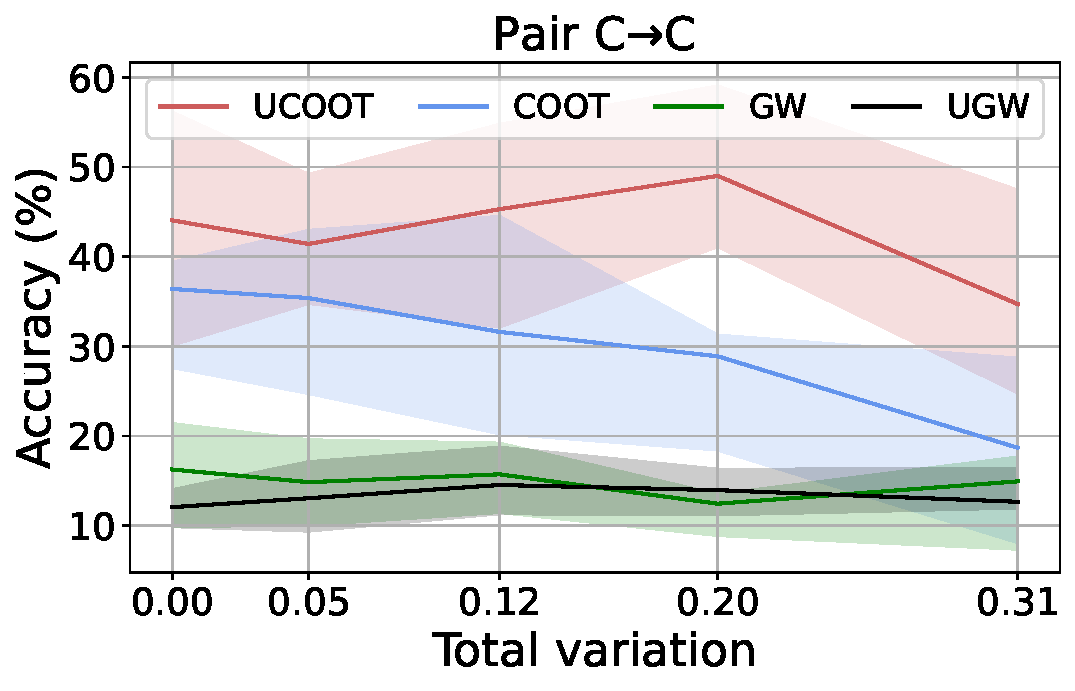
\includegraphics[width=\linewidth]{./Chapitre3/fig/summary_C_C.pdf}
  \vspace*{-7mm}
  \caption{Robustness to class proportion change for increasing TV on the class marginals.
  \label{f:hda_prop}}
\end{wrapfigure}
More precisely, we simulate a change in proportion only in the source domain
by selecting $20p$ samples per class for 4 amongst 10 classes with $p$
decreasing from $p=1$ to $p=0.2$. In this configuration,
the classes in the source domain are imbalanced and the unlabeled HDA problem becomes more difficult.
We report the performance of all the methods as a function of the Total Variation (TV)
between the class marginal distributions on one pair of datasets in \Cref{f:hda_prop}.
We can see that UCOOT is quite robust to change in class proportions,
while COOT experiences a sharp decrease in accuracy when the class distributions
become more imbalanced.

% We observe that in general, UCOOT is less stable than COOT, due to the mass
% relaxation nature. This is advantageous in the unsupervised HDA tasks, where, in absence of
% target labels, this relaxation provides flexibility to deals with the uncertainty of labels.
% For this reason, UCOOT usually outperforms COOT by large margins.
%
%\paragraph{Robustness to target shift}
%%%%%%%%%%%%%%%%%%%%%%%%%%%%%%%%%%%%%%%%%%%%
\subsubsection{Single-cell multi-omics alignment}

Finally, we present a real-world application of UCOOT for the alignment of single-cell measurements.
Recent advances in single-cell sequencing technologies allow biologists to measure
a variety of cellular features at the single-cell resolution, such as expression levels of genes
and epigenomic changes in the genome \citep{Buenrostro15,Chen19},
or the abundance of surface proteins \citep{CITEseq}. These multiple measurements produce
single-cell multi-omics datasets. These datasets measuring different biological phenomena
at the single-cell resolution allow scientists to study how the cellular processes are regulated,
leading to finer cell variations during development and diseases. However, it is hard to obtain
multiple types of measurements from the same individual cells due to experimental limitations.
Therefore, many single-cell multi-omics datasets have disparate measurements from different
sets of cells. As a result, computational methods are required to align the cells and
the features of the different measurements to learn the relationships between them that help
with data analysis and integration. Multiple tools \citep{Pamona, Seurat, Liu2019},
including GW \citep{Pamona, Demetci22} and UGW \citep{Demetci22-2} based methods,
have shown good performance for cell-to-cell alignments.
% However,  aligning both samples and features is a more challenging and critical task for this domain that can be solved by the UCOOT formulation.
However, aligning both samples and features is a more challenging and critical task that
GW and UGW-based methods cannot address
%\pinar{since they compute alignments between intra-domain distances, discarding features \citep{Demetci22, Pamona, Demetci22-2}}.
Here we provide an application of UCOOT to simultaneously align the samples and features
in a single-cell multi-omics dataset.
%
%how the features in different molecular features relate to one another.
%As a result, we require computational methods to align the cells and the features of the different measurements to obtain correspondence between similar cells and features. This correspondence information can help investigate which features in one domain (e.g., genes) match the ones (e.g., proteins) in the other domain.
%

\begin{figure}[t]
    \centering
    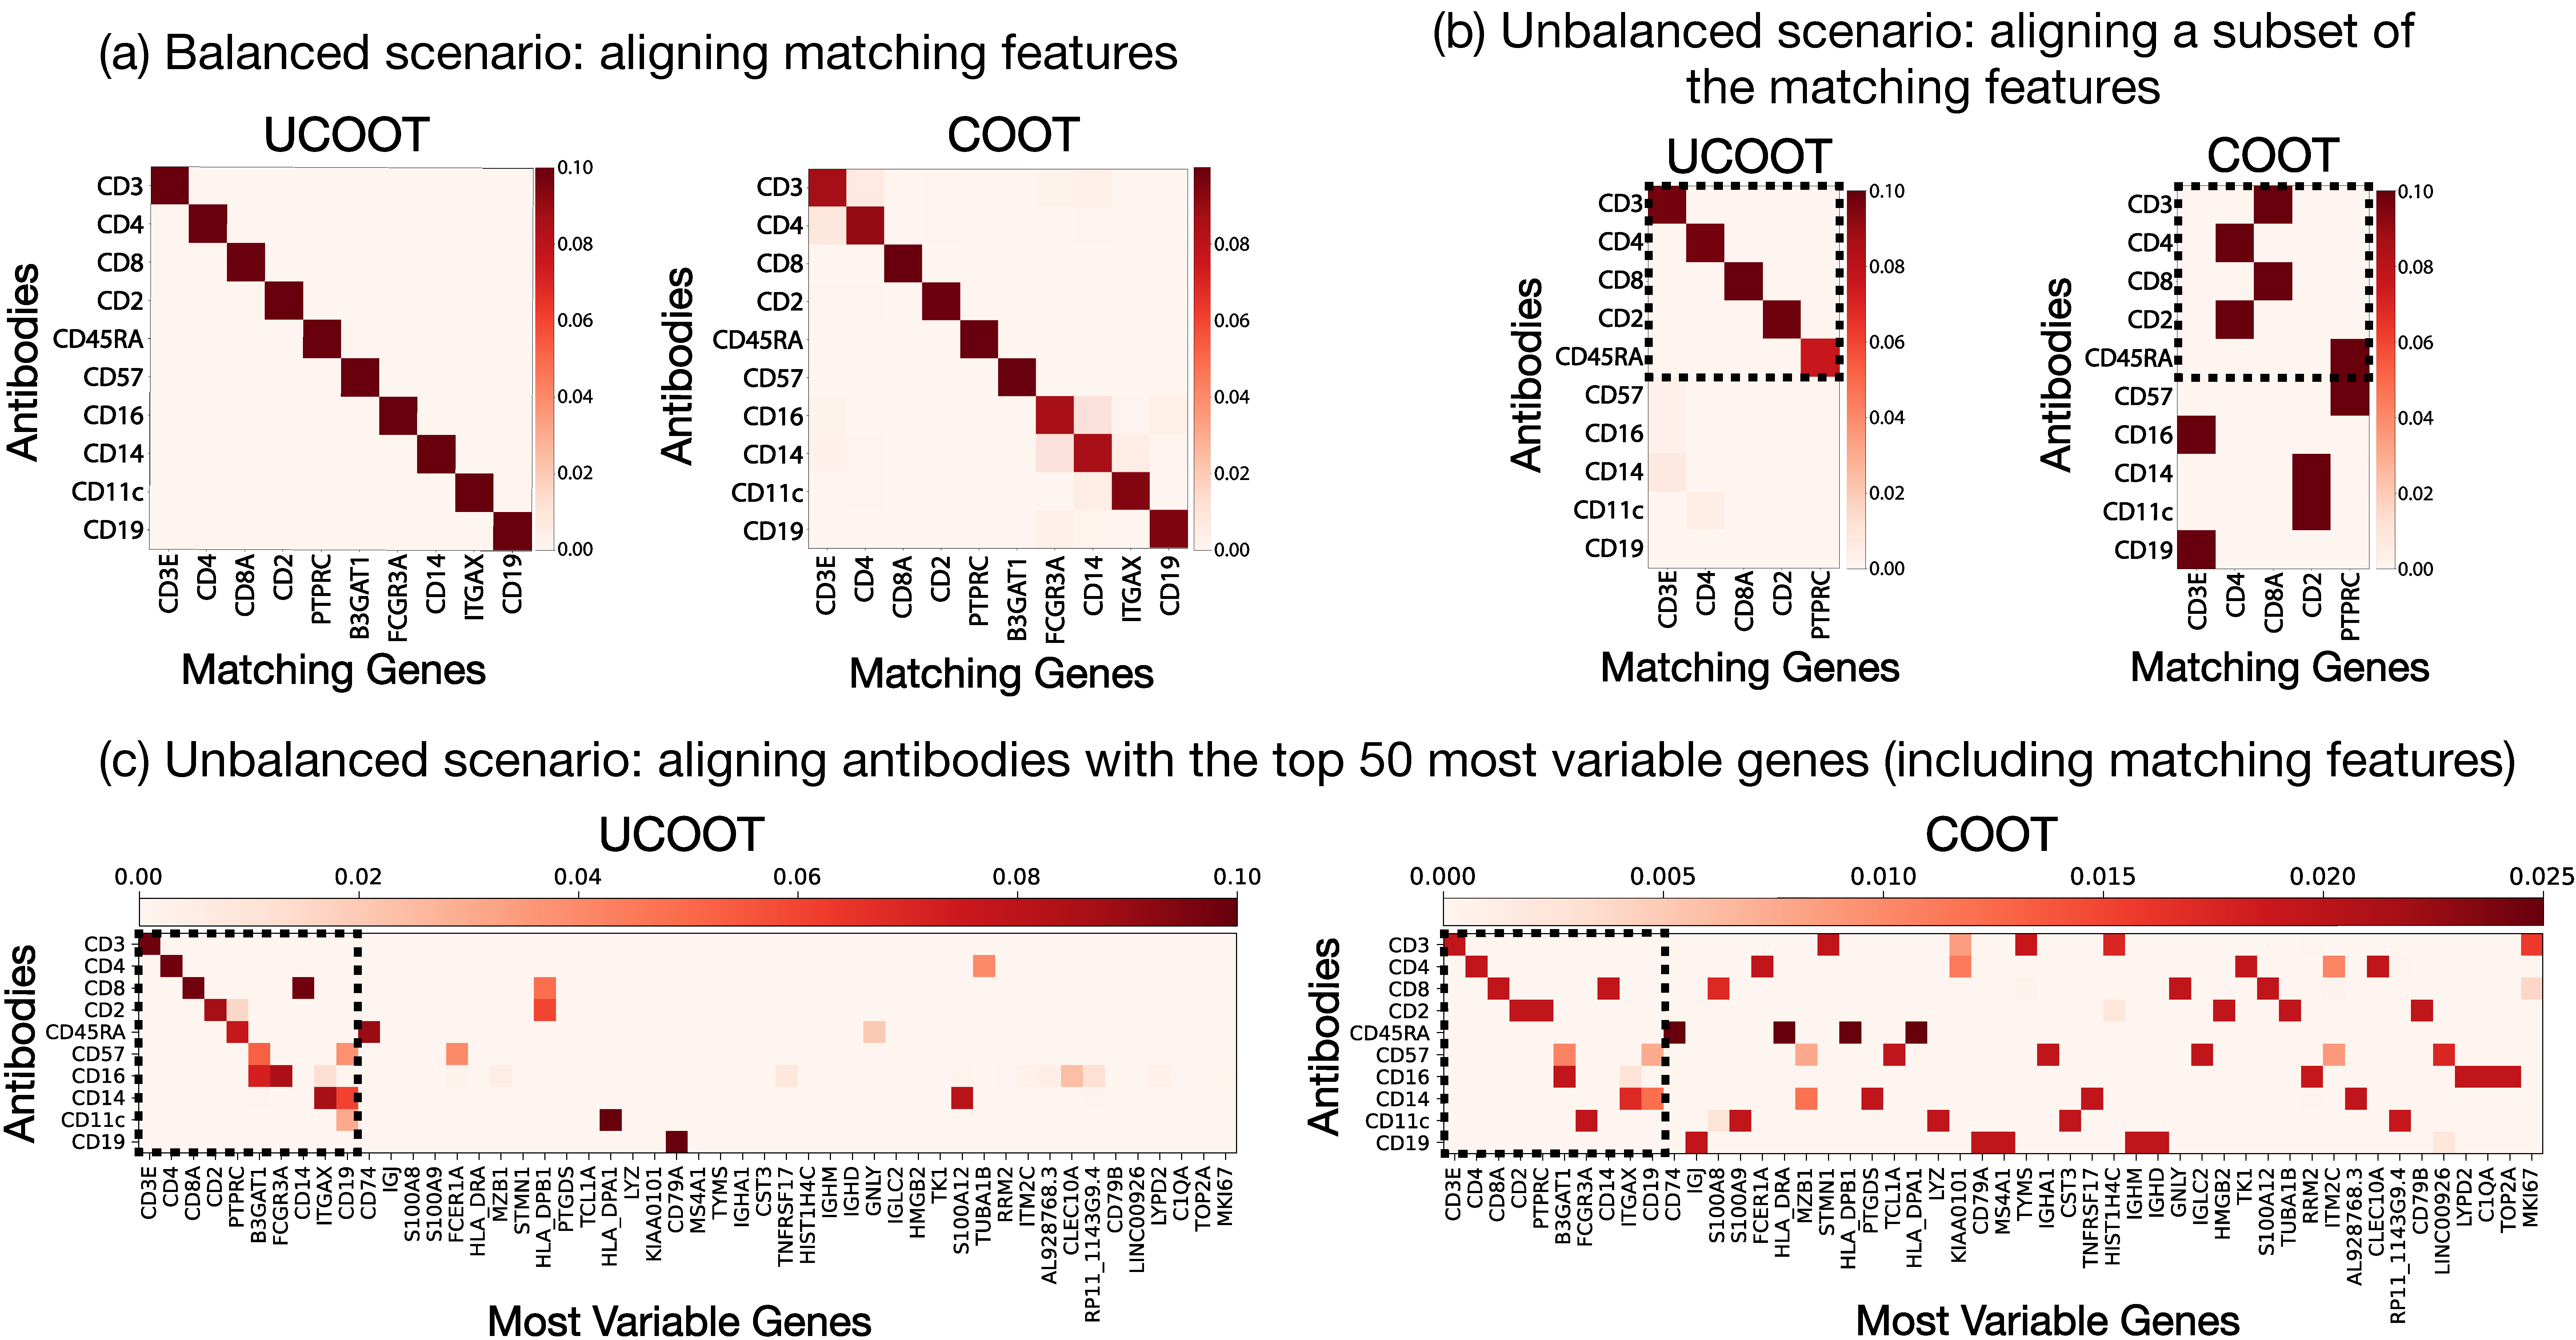
\includegraphics[trim={0.2cm 0.2cm 0.8cm 0.5cm}, clip, width=\linewidth, keepaspectratio=true]{./Chapitre3/fig/genes-alignments.pdf}
    \caption{Feature alignments on the single-cell multi-omics dataset of COOT and UCOOT between antibodies (surface proteins) and their matching genes (that encode them). \textbf{(a)} The features are sorted such that the correct alignment would yield a diagonal matrix. \textbf{(b)} Only five of the correct gene matches are kept (the last five genes from (a) are excluded). \textbf{(c)} Alignments between the ten antibodies and the top 50 most variable genes, including the matching genes.
    For \textbf{(b)} and \textbf{(c)}, the diagonal within the dashed square highlights the correct matches.
    Overall, UCOOT gives better feature alignments.
    \label{fig:multiomics}}
\end{figure}

\paragraph{Dataset} For demonstration, we choose a dataset generated by
the CITE-seq experiment \citep{CITEseq},
which simultaneously measures gene expression and antibody (or surface protein)
abundance in single cells. From this dataset, we use 1000 human peripheral blood cells,
which have ten antibodies and 17,014 genes profiled. We selected this specific dataset
as we know the ground-truth correspondences on both the samples (\ie, cells)
and the features (\ie, genes and their encoded antibodies), thus allowing us to quantify
and compare the alignment performance of UCOOT and COOT.
As done previously \citep{Pamona, Demetci22, Liu2019}, we quantify the cell alignment performance
by calculating the fraction of cells closer than the true match (FOSCTTM) of each cell
in the dataset and averaging it across all cells. This metric quantifies alignment error,
so lower values are more desirable. The feature alignments are measured by calculating
the accuracy of correct matching.

% \paragraph{Data Preprocessing} \label{CITEseq_exp_appendix}
% For the single-cell multi-omics experiments, we use the ``PBMC'' dataset from Stoeckius
% \textit{et al} \citep{CITEseq}, accessed on Gene Expression Omnibus (GEO) with the
% accession code: \href{https://www.ncbi.nlm.nih.gov/geo/query/acc.cgi?acc=GSE100866}{GSE100866}.
% This dataset contains a mix of 7,985 mouse and human peripheral blood mononuclear cells (PBMC)
% and profiles ten antibodies, 17,014 human genes, and 12,915 mouse genes. To pick the human cells,
% we follow the description in \citep{CITEseq}, and select the cells that have at least 500,
% and more than 90\% of all unique molecular identifiers (UMIs) mapped to the human genes
% (rather than the mouse genes). From the resulting $\sim 4500$ cells, we pick the first 1000
% to use in our experiments. We use the CLR-normalized antibody count data provided in GEO
% and apply log normalization to the gene expression data using Seurat package in R to
% remove biases in sequencing across cells \citep{Seurat}. Prior to alignment,
% we follow the existing single-cell alignment methods \citep{Demetci22, Demetci22-2,Liu2019,singh20},
% and also apply L2 normalization to both modalities. The top 50 most variable genes
% (\Cref{fig:multiomics}(c)) are selected using the \texttt{FindVariableFeatures()}
% function from \citep{Seurat}.

\paragraph{Hyperparameter tuning} Hyperparameters were tuned using grid search.
For both COOT and UCOOT, we considered the following range for the entropic regularization
coefficients $\varepsilon_f, \varepsilon_s \in \{1e-5, 5e-5, 1e-5, 5e-4, ... ,0.1, 0.5\}$.
For the mass relaxation coefficients $\rho_1, \rho_2 $ in UCOOT, the following range
was considered $\rho_1, \rho_2 \in \{1e-3, 5e-3, 0.01, 0.05, 0.1, 0.5, 1, 5, 10, 50 ,100\}$.
Each combination of hyperparameters were run on three randomly chosen subsets of the dataset
that included 30\% of the samples and the hyperparameter combinations that on average yielded
the highest feature matches and lowest FOSCTTM were picked for the experiments on the full dataset.

% I'll move the details about the original dataset to the Appendix
% The particular dataset we work with profiles a mix of 7,985 human and mouse peripheral blood mononuclear cells and contains measurements on 10 antibodies, 17014 human genes and 12915 mouse genes. We select 1000 human cells from this dataset to work with.

\paragraph{Results in balanced scenarios} First, we select and align the same number of samples and features
across the two datasets. For this, we subset the gene expression domain with the ten genes that
match to the ten antibodies they express. Original data contains the same number of cells
across domains since both domains are simultaneously measured in the same single-cells.
We observe that both UCOOT and COOT can correctly align features (\Cref{fig:multiomics}~(a))
and the cells across the two measurements. However,
UCOOT gives better performance, as demonstrated by a lower FOCSTTM score (0.0062 vs 0.0127)
for cells. Both COOT and UCOOT recover the diagonal for matching features (100\% accuracy),
but UCOOT recovers the exact matching, likely due to its robustness to noise,
whereas COOT assigns weights to other features as well.

\paragraph{Results in unbalanced scenarios} Next, we perform alignment with an unequal number of features.
This setting is more likely to occur for real-world single-cell datasets as different features
are measured. In the first simple scenario, we align the ten antibodies with only a subset (five)
of their matching genes. As visualized in \Cref{fig:multiomics}~(b),
COOT struggles to find the correct feature alignments (60\% accuracy),
which would lie in the diagonal of the highlighted square (dashed lines). However,
the relaxation of the mass conservation constraint in UCOOT allows it to shrink
the mass of antibodies that lack matches in the gene expression domain,
leading do higher accuracy (100\% accuracy).

Next, we align the ten antibodies with
the 50 most variable genes in the dataset, including their matching genes.
This alignment task is the most realistic scenario, as single-cell multi-omics data
consists of high-dimensional datasets with a different number of features for different measurements.
% \pinar{Moreover, many of these genes show consistent expression levels across }
Therefore, biologists focus their analyses on the reduced set of most variable features (e.g. genes).
It is also the most computationally challenging case among all our experiments on this dataset.
Hence, we provide sample-level supervision to both methods by giving a cost penalization matrix
based on the correct sample alignments to the sample alignment computation.
We see in \Cref{fig:multiomics}(c) that in comparison to COOT (50\% accuracy),
UCOOT recovers more of the correct feature alignments (70\% accuracy),
and yields fewer redundant alignments.
Note that UCOOT avoids incorrect mappings by locally shrinking the mass of the features or samples
that lack correspondences. This avoids subsequent incorrect downstream analysis of
the integration results. This property can also help users to discover rare cell types
by observing the extent of mass relaxation per cell or prune uninformative features in
the single-cell datasets.

%Similarly to the alignment in \Cref{fig:multiomics}(b), this is thanks to the mass shrinkage of the features that lack correspondences. By locally adjusting the mass in transport, UCOOT tends to avoid assigning correspondences to samples or features that lack matches across the aligned domains. With this, UCOOT can help users to detect outliers that can result from experimental artifacts,
%(such as rare cell types or lowly expressed genes that are not captured well by a sequencing technology), prune features or discover rare cell types.}

Lastly, we also consider the case of unequal number of samples across the two measurements.
This case is common in real world single-cell multi-omics datasets that are not
simultaneously measured. \citet{Demetci22-2} have shown that
single-cell alignment methods that do not account for this mismatch yield poor alignment results.
Therefore, we downsample the number of cells in one of the domains by 25\%
and perform alignment with the full set of cells in the other domain.
We compute the FOSCTTM score for all cells that have a true match in the dataset and
report the average values. UCOOT continues to yield a low FOSCTTM score (0.0081 compared to 0.0062
in the balanced scenario), while COOT shows a larger drop in performance
(0.1342 compared to 0.0127 in the balanced scenario).

\subsection{Discussion and conclusion}
\label{sec:conclusion}

In this work, we present an extension of COOT called unbalanced COOT,
where the hard constraint on the marginal distributions is replaced by a soft control via
the KL divergence. The resulting problem not only benefits from the flexibility of COOT
but also enjoys the provable robustness property under the presence of outliers,
which is not the case for COOT. The experimental results confirm our findings,
yielding a very competitive performance in the unsupervised HDA task, as well as
meaningful feature couplings for the single-cell multi-omics alignment. Also,
while UCOOT introduces additional hyper-parameters, domain knowledge can help narrow down
the range of feasible values, thus reducing the time and computational cost of the tuning process.
Further investigation should be carried out to fully understand and assess
the observed efficiency of UCOOT in real-world applications,
and also explore the possibilities of UCOOT in more diverse applicative settings,
including its use as a loss in deep learning architectures.
Lastly, from a theoretical perspective, statistical properties such as
sample complexity or stability analysis are needed to better understand
the intricate relations between the two sample and feature couplings.
%Future works may also focus on justifying how the relaxation of marginal constraints allows to cope with the class imbalance and provides empirically better initialization to the approximation scheme of COOT, as observed in the experiments. Last but not least, it is interesting to study the connection with the unbalanced GW distance, since in practice, it is estimated using its lower bound, which is in fact a special of UCOOT.

% The last section presents the results from \citep{Thual22} and addresses the applications of
% unbalanced extension of fused Gromov-Wasserstein in human brains alignments.
% Individual brains vary in both anatomy and functional organization, even within a given species.
% Inter-individual variability is a major impediment when trying to draw generalizable conclusions
% from neuroimaging data collected on groups of subjects.
% Current co-registration procedures rely on limited data, and thus lead to very coarse
% inter-subject alignments.
% In this work, we present a novel method for inter-subject alignment based on Optimal Transport,
% denoted as Fused Unbalanced Gromov-Wasserstein (FUGW).
% The method aligns cortical surfaces based on the similarity of their functional signatures in
% response to a variety of stimulation settings, while penalizing large deformations of
% individual topographic organization.
% We demonstrate that FUGW is well-suited for whole-brain landmark-free alignment.
% The unbalanced feature allows to deal with the fact that functional areas
% vary in size across subjects. Our results show that FUGW alignment significantly
% increases between-subject correlation of activity for independent functional data,
% and leads to more precise mapping at the group level.

% 
%%%%%%%%%%%%%%%%%%%%%%%%%%%%%%%%%%%%%%%%%%%%%%
\section{Inexact Bregman Proximal Point for Entropic Unbalanced Optimal Transport}
\label{sec:input}

This section is an ongoing work on an alternative solver for the entropic UOT problem
\ref{eq:discrete_ent_uot}, which has not yet been studied in the literature,
to the best of our knowledge.
We called this approach \textit{INexact Proximal Unbalanced optimal Transport} (INPUT),
since it is a straightforward application of the inexact Bregman Proximal Point (BPP) algorithm
to the UOT problem. We present the derivation of INPUT, then illustrate how
it can overcome the limitations of the MM and Sinkhorn-based methods,
while being orders of magnitude faster in our toy experiments. Despite the simplicity,
its convergence analysis remains a challenging open problem and is under our active research.

\subsection{Motivation, optimization and algorithm}

While the Bregman Proximal Point method \citep{Chen93} applies to the class of Bregman divergences,
we will exclusively focus on the KL divergence throughout this thesis.
\begin{definition}
  Given a nonepmpty closed convex set of $E \subset \bbR^d_{\geq 0}$
  and a proper closed convex function $f: E \to \bbR$, consider the following
  convex optimization problem
  \begin{align}
    \min_{x \in E} f(x).
  \end{align}
  For learning rate $\eta > 0$, the exact BPP scheme with respect to the KL divergence reads
  \begin{align}
    \label{eq:bppa}
    x^{(t+1)} = \argmin_{x \in E} f(x) + \eta \kl(x, x^{(t)}),
  \end{align}
  and the inexact BPP scheme reads
  \begin{align}
    \label{eq:bppa_inexact}
    x^{(t+1)} \approx \argmin_{x \in E} f(x) + \eta \kl(x, x^{(t)}).
  \end{align}
  Here, $x^{(t+1)}$ is only an approximate solution in some predefined sense.
\end{definition}
When applying to Problem \eqref{eq:discrete_ent_uot}, the exact BPP iteration boils down to solving
\begin{align}
\label{eq:bpp_uot}
  &P^{(t+1)} \\
  &= \argmin_{P \in \bbR^{m \times n}_{\geq 0}}
  \langle C, P \rangle + \rho_1 \kl(P_{\# 1} | \mu)
  + \rho_2 \kl(P_{\# 2} | \nu) + \varepsilon \kl(P | \gamma) + \eta \kl(P | P^{(t)}) \\
  &= \argmin_{P \in \bbR^{m \times n}_{\geq 0}}
  \left \langle C - \eta \log \frac{P^{(t)}}{\gamma}, P \right \rangle
  + \rho_1 \kl(P_{\# 1} | \mu) + \rho_2 \kl(P_{\# 2} | \nu) + (\varepsilon + \eta) \kl(P | \gamma).
\end{align}
This is nothing but an entropic UOT problem with modified cost and regularization.
Thus, any solvers discussed in \Cref{sub:uot_optim} can be used. In particular,
by construction, BPP is naturally applicable to the unregularized UOT.
In practice, the exact BPP may not be an efficient algorithm to solve the UOT problem since
it requires solving \textbf{exactly} many entropic subproblems. This can be computationally expensive,
especially when the learning rate is small.

While the inexact BPP scheme has recently been applied to the balanced OT \citep{Xie20,Yang22},
we are not aware of any extension to the unbalanced counterpart.
Our proposed method follows directly from \citep{Xie20}, which is simple to implement and
usually performs well in practice. In particular,
we only require running a few Sinkhorn iterations for each entropic subproblem and
use the approximated coupling as input for the next BPP iteration.
The algorithmic details of INPUT can be found in \Cref{alg:isppa}.
\begin{algorithm}[t]
  \caption{INPUT algorithm for Problem \eqref{eq:discrete_ent_uot}.}
  \label{alg:isppa}
\begin{algorithmic}[1]
  \STATE \textbf{Input:} cost matrix $C \in \bbR^{m \times n}$,
  measures $\mu \in \bbR^m_{> 0}, \nu \in \bbR^n_{> 0}, \gamma \in \bbR^{m \times n}_{> 0}$,
  regularization $\varepsilon \geq 0$, relaxation parameters $\rho_1, \rho_2 > 0$,
  learning rate $\eta > 0$.
  \FOR{$t=1, \dots, T$}
  \STATE Calculate new cost: $C^{(t+1)} \gets C - \eta \log \Big( \frac{P^{(t)}}{\gamma} \Big)$.
  \STATE Solve approximatively the entropic UOT problem
  \begin{align}
    P^{(t+1)} \approx \argmin_{P \geq 0} \; \langle C^{(t+1)}, P \rangle +
    \rho_1 \kl(P_{\# 1} | \mu) + \rho_2 \kl(P_{\# 2} | \nu) + (\varepsilon + \eta) \kl(P | \gamma).
  \end{align}
  \ENDFOR
  \STATE \textbf{Output:} transport plan $P^{(T)}$.
\end{algorithmic}
\end{algorithm}

\subsection{Convergence analysis in the exact setting}

Let us start with the convergence analysis in case of exact BPP iteration \ref{eq:bpp_uot}.
Thanks to Lemma 3.3 and Theorem 3.4 in \citep{Chen93}, if $P^*$ is a minimizer of
Problem \eqref{eq:discrete_ent_uot}, then
\begin{enumerate}
  \item The sequence $\big( \kl(P^*, P^{(t)}) \big)_t$ is nonincreasing and converges to $0$.
  \item The sequence $\big( F(P^{(t)}) \big)_t$ is nonincreasing and
  \begin{align}
    \label{eq:chen_teboulle}
    F(P^{(t)}) - F(P^*) \leq \frac{\eta}{t} \kl(P^* | P^{(0)}).
  \end{align}
\end{enumerate}
The upper bound \eqref{eq:chen_teboulle} can be improved by further exploiting the property of
the objective function of Problem \eqref{eq:discrete_ent_uot}.
First, we introduce the notions of relative smoothness \citep{Bauschke17} and
strong convexity \citep{Lu18} of a function with respect to the KL divergence.
\begin{definition}
  \label{def:smooth-convex}
  Let $f:C \to \bbR$ be a differentiable convex function.
  Given $L \geq 0$, we say that $f$ is $L-$smooth relative to the KL divergence
  if for any $x, y \in C$,
  \begin{align}
    f(x) \leq f(y) + \langle \nabla f(y), x - y \rangle + L \; \kl(x, y).
  \end{align}
  Given $l \geq 0$, we say $f$ is $l-$strongly convex relative to the KL divergence
  if for any $x, y \in C$,
  \begin{align}
    f(x) \geq f(y) + \langle \nabla f(y), x - y \rangle + l\; \kl(x, y).
  \end{align}
\end{definition}

\begin{lemma}
  \label{lemma:convex-smoothness}
  $F$ is $\varepsilon$-strongly convex and $(\lambda_1 + \lambda_2 + \varepsilon)$-relatively smooth
  with respect to the KL divergence.
\end{lemma}
The following result is a simple generalization of Theorem 3.1 in \citep{Lu18}.
\begin{proposition}[Convergence rate of exact BPP for Problem \eqref{eq:discrete_ent_uot}]
  \label{prop:convergence-exact-sppa}
  For every $\eta > 0$, exact BPP scheme decreases the value of $F(\cdot)$ with each iteration $t$:
  the sequence $\big( F(\pi^{(t)}) \big)_t$ is monotonically decreasing.
  Moreover, if $\varepsilon \leq \eta \leq \lambda_1 + \lambda_2 + \varepsilon$,
  then we have
  \begin{align}
    F(\pi^{(t)}) - F(\pi^*)
    \leq \frac{\varepsilon}{\left( 1 +
    \frac{\varepsilon (\lambda_1 + \lambda_2 + \varepsilon)}{\eta (\lambda_1 + \lambda_2)} \right)^t - 1}
    \kl(\pi^* | \pi^{(0)}).
  \end{align}
\end{proposition}
It is not difficult to check that this bound is weaker than the one in
Inequality (\ref{eq:chen_teboulle}). Indeed,
\begin{align}
  \frac{\varepsilon}{\left( 1 +
  \frac{\varepsilon (\lambda_1 + \lambda_2 + \varepsilon)}{\eta (\lambda_1 + \lambda_2)} \right)^t - 1}
  \leq \frac{\varepsilon}{\frac{t \varepsilon(\lambda_1 + \lambda_2 + \varepsilon)}{\eta (\lambda_1 + \lambda_2)}}
  = \frac{\eta}{t} \frac{\lambda_1 + \lambda_2}{\lambda_1 + \lambda_2 + \varepsilon}
  \leq \frac{\eta}{t}.
\end{align}

\subsection{Convergence analysis in the inexact setting}

Despite the simplicity, it is difficult to analyze the convergence of INPUT.
In particular, while it is an immediate extension of the work of \citet{Xie20} on the balanced OT,
their proof techniques of the convergence can not be adapted to the unbalanced setting.
This is because they rely on the property of the set of admissible couplings,
which is not available in the UOT. Moreover, their assumptions and conditions are also
not trivial to verify in practice, thus the convergence results are mostly of theoretical interest.

The convergence analysis of the inexact BPP has already been studied at the same time
as the exact one. Typically, one can control the approximation error using
$\varepsilon$-subdifferential \citep{Burachik97,Kiwiel97},
or bounded subgradient \citep{Eckstein98,Rockafellar76}, to name a few.
We are studying the literature in this domain to identify the relevant criteria, which are
amenable to study the convergence and to verify in practice.

\subsection{Illustration on toy example}

\paragraph{Experimental setup}
We consider a synthetic dataset:
the source data $X$ contains $200$ points forming an ellipse and a square,
assigned with the same uniform probability on both shapes
$\mu = \frac{1}{200} \sum_{i=1}^{200} \delta_{x_i}$. The target data $Y$ also contains $200$ points
forming an ellipse and a circle, assigned with the histogram
$\nu = \frac{3}{200} \sum_{j=1}^{30} \delta_{y_j \in \text{Circle}} +
\frac{7}{200} \sum_{j=31}^{100} \delta_{y_j \in \text{Circle}} +
\frac{7}{200} \sum_{j=1}^{100} \delta_{y_j \in \text{Ellipse}}$.
The objective in this experiment is to estimate the entropic UOT cost, where
we choose $\gamma = \mu \otimes \nu$ and the cost $C(x, y) = || x - y||^2_2$.

\paragraph{Competing methods}
For INPUT, we consider $3$ versions corresponding to $3$ solvers for the inner entropic UOT problem:
\texttt{INPUT-Sinkhorn}, \texttt{INPUT-TI-v2}, \texttt{INPUT-MM}.
Here, we choose the variant of Sinkhorn-TI (\Cref{alg:TI_Sinkhorn_variant})
since it is more simple to implement, yet appears to perform comparably to the Sinkhorn-TI.
The Sinkhorn-based methods include
\texttt{Sinkhorn} (\Cref{alg:Sinkhorn_algo}), \texttt{Sinkhorn-TI-v1} (\Cref{alg:TI_Sinkhorn})
and its variant \texttt{Sinkhorn-TI-v2} (\Cref{alg:TI_Sinkhorn_variant}).
We emphasize that all Sinkhorn-based methods require log-domain implementation
for numerical stability, whereas INPUT does not suffer this issue,
thus is implemented with direct vector-matrix multiplication.
Apart from these $2$ families of solvers, we also evaluate the performance of
Majorization-Minimization algorithm \texttt{MM}.

\paragraph{Results}
We set up $4$ scenarios to verify if INPUT can overcome the limitations of other existing methods.
More precisely, the first one considers the situation of small relaxations and large regularization.
It is an easy test and we expect that all methods perform well.
In the second one, we fix the relaxations but choose small regularization
in order to hinder convergence of Sinkhorn-based methods.
The third scenario uses fixed regularization but very large marginal relaxations to slow down
the convergence of MM.
The last one combines small regularization and very large relaxations. It is designed to challenge
both Sinkhorn and MM methods.

It is clear that the INPUT family consistently and significantly outperforms other solvers,
The distinction becomes even more visible in the regimes where Sinkhorn and MM struggle.
Except for the first scenario, by contrast to its competitors,
it seems that INPUT does not require compensating the running time for the quality of the estimation.
We also observe that, within the family of INPUT,
combining INPUT with Sinkhorn-TI yields the most efficient algorithm.
Amongst the Sinkhorn-based solvers, Sinkhorn-TI shows clear improvement over Sinkhorn,
even though this advantage quickly diminishes when regularization is small.

\begin{table}[]
  \small
  \centering
  \begin{tabular}{|cc|c|c|c|c|}
  \hline
  \multicolumn{2}{|c|}{} &
    \textbf{\begin{tabular}[c]{@{}c@{}}Scenario 1\\ $\rho_1 = 40$\\ $\rho_2 = 50$\\ $\varepsilon = 1$\end{tabular}} &
    \textbf{\begin{tabular}[c]{@{}c@{}}Scenario 2\\ $\rho_1 = 40$\\ $\rho_2 = 50$\\ $\varepsilon = 1e-3$\end{tabular}} &
    \textbf{\begin{tabular}[c]{@{}c@{}}Scenario 3\\ $\rho_1 = 4000$\\ $\rho_2 = 5000$\\ $\varepsilon = 1$\end{tabular}} &
    \textbf{\begin{tabular}[c]{@{}c@{}}Scenario 4\\ $\rho_1 = 4000$\\ $\rho_2 = 5000$\\ $\varepsilon = 1e-3$\end{tabular}} \\ \hline
  \multicolumn{1}{|c|}{\multirow{3}{*}{\textbf{\begin{tabular}[c]{@{}c@{}}Sinkhorn\\ family\end{tabular}}}} &
    \textbf{Sinkhorn} &
    \begin{tabular}[c]{@{}c@{}}0.275 $\pm$ 0.011\\ {\color{blue}{{41.618}}} \end{tabular} &
    \begin{tabular}[c]{@{}c@{}}55.946 $\pm$ 5.893\\ 40.588\end{tabular} &
    \begin{tabular}[c]{@{}c@{}}{\color{red}{{0.020 $\pm$ 0.002}}} \\ 57.667\end{tabular} &
    \begin{tabular}[c]{@{}c@{}}No convergence at \\ this tolerance\end{tabular} \\ \cline{2-6}
  \multicolumn{1}{|c|}{} &
    \textbf{TI-v1} &
    \begin{tabular}[c]{@{}c@{}}0.389 $\pm$ 0.018\\ {\color{blue}{{41.618}}}\end{tabular} &
    \begin{tabular}[c]{@{}c@{}}37.679 $\pm$ 0.926\\ {\color{red}{{40.576}}}\end{tabular} &
    \begin{tabular}[c]{@{}c@{}}1.118 $\pm$ 0.047\\ 57.613\end{tabular} &
    \begin{tabular}[c]{@{}c@{}}31.088 $\pm$ 0.505\\ 56.834\end{tabular} \\ \cline{2-6}
  \multicolumn{1}{|c|}{} &
    \textbf{TI-v2} &
    \begin{tabular}[c]{@{}c@{}}0.318 $\pm$ 0.013\\ {\color{blue}{{41.618}}}\end{tabular} &
    \begin{tabular}[c]{@{}c@{}}31.679 $\pm$ 2.919\\ {\color{red}{{40.576}}}\end{tabular} &
    \begin{tabular}[c]{@{}c@{}}0.871 $\pm$ 0.034\\ 57.613\end{tabular} &
    \begin{tabular}[c]{@{}c@{}}24.828 $\pm$ 0.243\\ 56.834\end{tabular} \\ \hline
  \multicolumn{1}{|c|}{\multirow{3}{*}{\textbf{\begin{tabular}[c]{@{}c@{}}INPUT\\ family\end{tabular}}}} &
    \textbf{Sinkhorn} &
    \begin{tabular}[c]{@{}c@{}}0.190 $\pm$ 0.008\\ {\color{blue}{{41.618}}}\end{tabular} &
    \begin{tabular}[c]{@{}c@{}}0.676 $\pm$ 0.032\\ {\color{blue}{{40.521}}}\end{tabular} &
    \begin{tabular}[c]{@{}c@{}}1.143 $\pm$ 0.048\\ {\color{blue}{{57.608}}}\end{tabular} &
    \begin{tabular}[c]{@{}c@{}}1.387 $\pm$ 0.026\\ {\color{blue}{{55.866}}}\end{tabular} \\ \cline{2-6}
  \multicolumn{1}{|c|}{} &
    \textbf{TI-v2} &
    \begin{tabular}[c]{@{}c@{}}{\color{red}{{0.149 $\pm$ 0.008}}}\\ {\color{blue}{{41.618}}} \end{tabular} &
    \begin{tabular}[c]{@{}c@{}}{\color{red}{{0.649 $\pm$ 0.013}}}\\ {\color{blue}{{40.521}}} \end{tabular} &
    \begin{tabular}[c]{@{}c@{}}{\color{blue}{{0.018 $\pm$ 0.002}}} \\ {\color{red}{{57.609}}}\end{tabular} &
    \begin{tabular}[c]{@{}c@{}}{\color{blue}{{0.079 $\pm$ 0.010}}} \\ {\color{red}{{55.868}}}\end{tabular} \\ \cline{2-6}
  \multicolumn{1}{|c|}{} &
    \textbf{MM} &
    \begin{tabular}[c]{@{}c@{}} {\color{blue}{{0.068 $\pm$ 0.006}}} \\ 41.627\end{tabular} &
    \begin{tabular}[c]{@{}c@{}} {\color{blue}{{0.186 $\pm$ 0.007}}} \\ 40.640\end{tabular} &
    \begin{tabular}[c]{@{}c@{}}1.038 $\pm$ 0.026\\ 57.738\end{tabular} &
    \begin{tabular}[c]{@{}c@{}}1.028 $\pm$ 0.021\\ 56.723\end{tabular} \\ \hline
  \multicolumn{2}{|c|}{\textbf{MM}} &
    \begin{tabular}[c]{@{}c@{}}0.193 $\pm$ 0.010\\ {\color{red}{{41.621}}} \end{tabular} &
    \begin{tabular}[c]{@{}c@{}}0.864 $\pm$ 0.024\\ 40.558\end{tabular} &
    \begin{tabular}[c]{@{}c@{}}0.726 $\pm$ 0.046\\ 59.089\end{tabular} &
    \begin{tabular}[c]{@{}c@{}}{\color{red}{{0.944 $\pm$ 0.026}}} \\ 57.829\end{tabular} \\ \hline
  \end{tabular}
  \caption{Time $\pm$ standard deviation (in seconds) required to reach the predefined tolerance
  (first line) and entropic UOT cost (second line). The lower score the better.
  {\color{blue}{{Blue number}}} indicates the best score.
  {\color{red}{{Red number}}} indicates the second best score.
  \label{t:uot_time_compare}}
\end{table}

\subsection{Discussion}

While this experiment is mainly for the proof-of-concept purpose,
it shows that INPUT is a promising alternative solver for the UOT problem.

\paragraph{Strengths of INPUT}
INPUT has two very appealing features. First, it overcomes the limitations of
the MM and Sinkhorn-based algorithms. In particular,
it can, not only handle both balanced/unbalanced, and unregularized/regularized settings,
but also, empirically, can converge very fast to the optimal plan and the global minimum,
even in the regimes of very small regularization (where Sinkhorn-based methods struggles),
or of very large relaxation (where MM wrestles).
We summarize the applicability of these algorithms in \Cref{t:uot_algo_compare}.

Second, the presence of learning rate $\eta$
increases the level of regularization in the inner entropic UOT subproblem,
thus brings two important benefits. The first one is on the reduction of number of iterations:
the larger the regularization, the faster the Sinkhorn algorithm converges. As a consequence,
running only a few iterations is usually enough to obtain a decent approximation of
the true solution. The second advantage is on the acceleration per BPP iteration. In practice,
when the regularization is not too small, one can ignore the log-domain implementation
and employ the one with direct vector-matrix multiplication,
without any concern about the numerical overflow issue.
As a result, this allows to speed up the calculation of the iterates.

\paragraph{Weaknesses of INPUT} There is no free lunch. INPUT has two drawbacks.
First, the cost matrix must be recalculated at the beginning of each BPP iteration.
This can be computationally expensive and prevents INPUT from being scalable.
Second, while tuning the learning rate is neither too tricky nor difficult,
it may take some effort to find an appropriate value. One possible workaround,
which usually works well in practice, is to start with $\eta$ small and not too far from $\varepsilon$.
The intuition of this heuristic comes from \Cref{prop:convergence-exact-sppa} of exact BPP scheme,
which indicates that, for fixed initialization, the smaller the learning rate, the smaller
the potential gap between the estimation and the minimum.
\begin{table}[t]
	\centering
		\begin{tabular}{|l|c|c|c|c|}
    \hline
    & \textbf{\makecell{Scaling}}
    & \textbf{\makecell{TI-Sinkhorn}} & \textbf{MM} & \textbf{INPUT} \\
    \hline
    \makecell[l]{Unregularized \\ setting} & \nomark & \nomark & \yesmark & \yesmark \\
    \hline
    \makecell[l]{Balanced \\ setting} & \yesmark & \yesmark & \nomark  & \yesmark  \\
    \hline
    \makecell[l]{Semi-relaxed \\ setting} & \yesmark & \yesmark & \nomark  & \yesmark  \\
    \hline
    \makecell[l]{Major \\ drawbacks} & \makecell{Very slow conv. \\ for small $\varepsilon$}
    & \makecell{Slow conv. \\ for small $\varepsilon$}
    & \makecell{Slow conv. \\ for large $\rho$}
    & \makecell{Cost recalculation, \\
    extra tuning of \\ hyperparameters} \\
    \hline
		\end{tabular}
		\caption{Summary of features of algorithms for entropic UOT problem \eqref{eq:discrete_ent_uot}.
    Unregularized setting refers to $\varepsilon = 0$, balanced setting corresponds to
    $\rho_1 = \rho_2 = \infty$ and semi-relaxed setting refers to either $\rho_1 = \infty$
    or $\rho_2 = \infty$.
    \label{t:uot_algo_compare}}
\end{table}

\paragraph{Can we adapt INPUT to solve the squared $l_2$-regularized Problem \eqref{uot_l2} ?}
In theory, yes, since the squared $l_2$-norm is a Bregman divergence,
thus the (inexact) BPP scheme is applicable. However, comparing to the MM solver,
we doubt that it would bring any gain in convergence speed. Indeed,
recall that the main motivation of INPUT comes from the poor convergence behavior of Sinkhorn
algorithm when \textbf{regularization} is small. For this reason, adding more regularization
to each BPP iteration helps accelerating the calculation
and improving the convergence of the algorithm. By contrast,
the case of squared $l_2$-norm does not suffer the same issue,
but rather on the \textbf{relaxation} parameters. So, more regularization does not help.
% \section{Fused Unbalanced Gromov-Wasserstein}

%%%%%%%%%%%%%%%%%%%%%%%%%%%
\subsection{Introduction}
\label{sec:introduction}

The availability of millimeter or sub-millimeter anatomical or functional brain images has opened
new horizons to
neuroscience, namely that of mapping cognition in the human brain and detecting markers of diseases.
%
Yet this endeavour has stumbled on the roadblock of inter-individual
variability: while the overall organization of the human brain is largely invariant,
two different brains (even from monozygotic twins \citep{pizzigali2020})
may differ at the scale of centimeters in shape, folding pattern, and functional responses.
%
% While variability is a hindrance to brain mapping,
The problem is further complicated by the fact that functional images
are noisy, due to imaging limitations and behavioral
differences across individuals that cannot be easily overcome.
%
The status quo of the field is thus to rely on anatomy-based inter-individual alignment
that approximately matches the outline of the brain \citep{ants}
as well as its large-scale cortical folding patterns \citep{fs_reconall,fischl_freesurfer_2012}.
%
Existing algorithms thus coarsely match anatomical features with diffeomorphic transformations,
by warping individual data to a simplified template brain.
Such methods lose much of the original individual detail and blur the functional information
that can be measured in brain regions (see \Cref{fig:intro}).

\begin{figure}[ht]
    \centering
    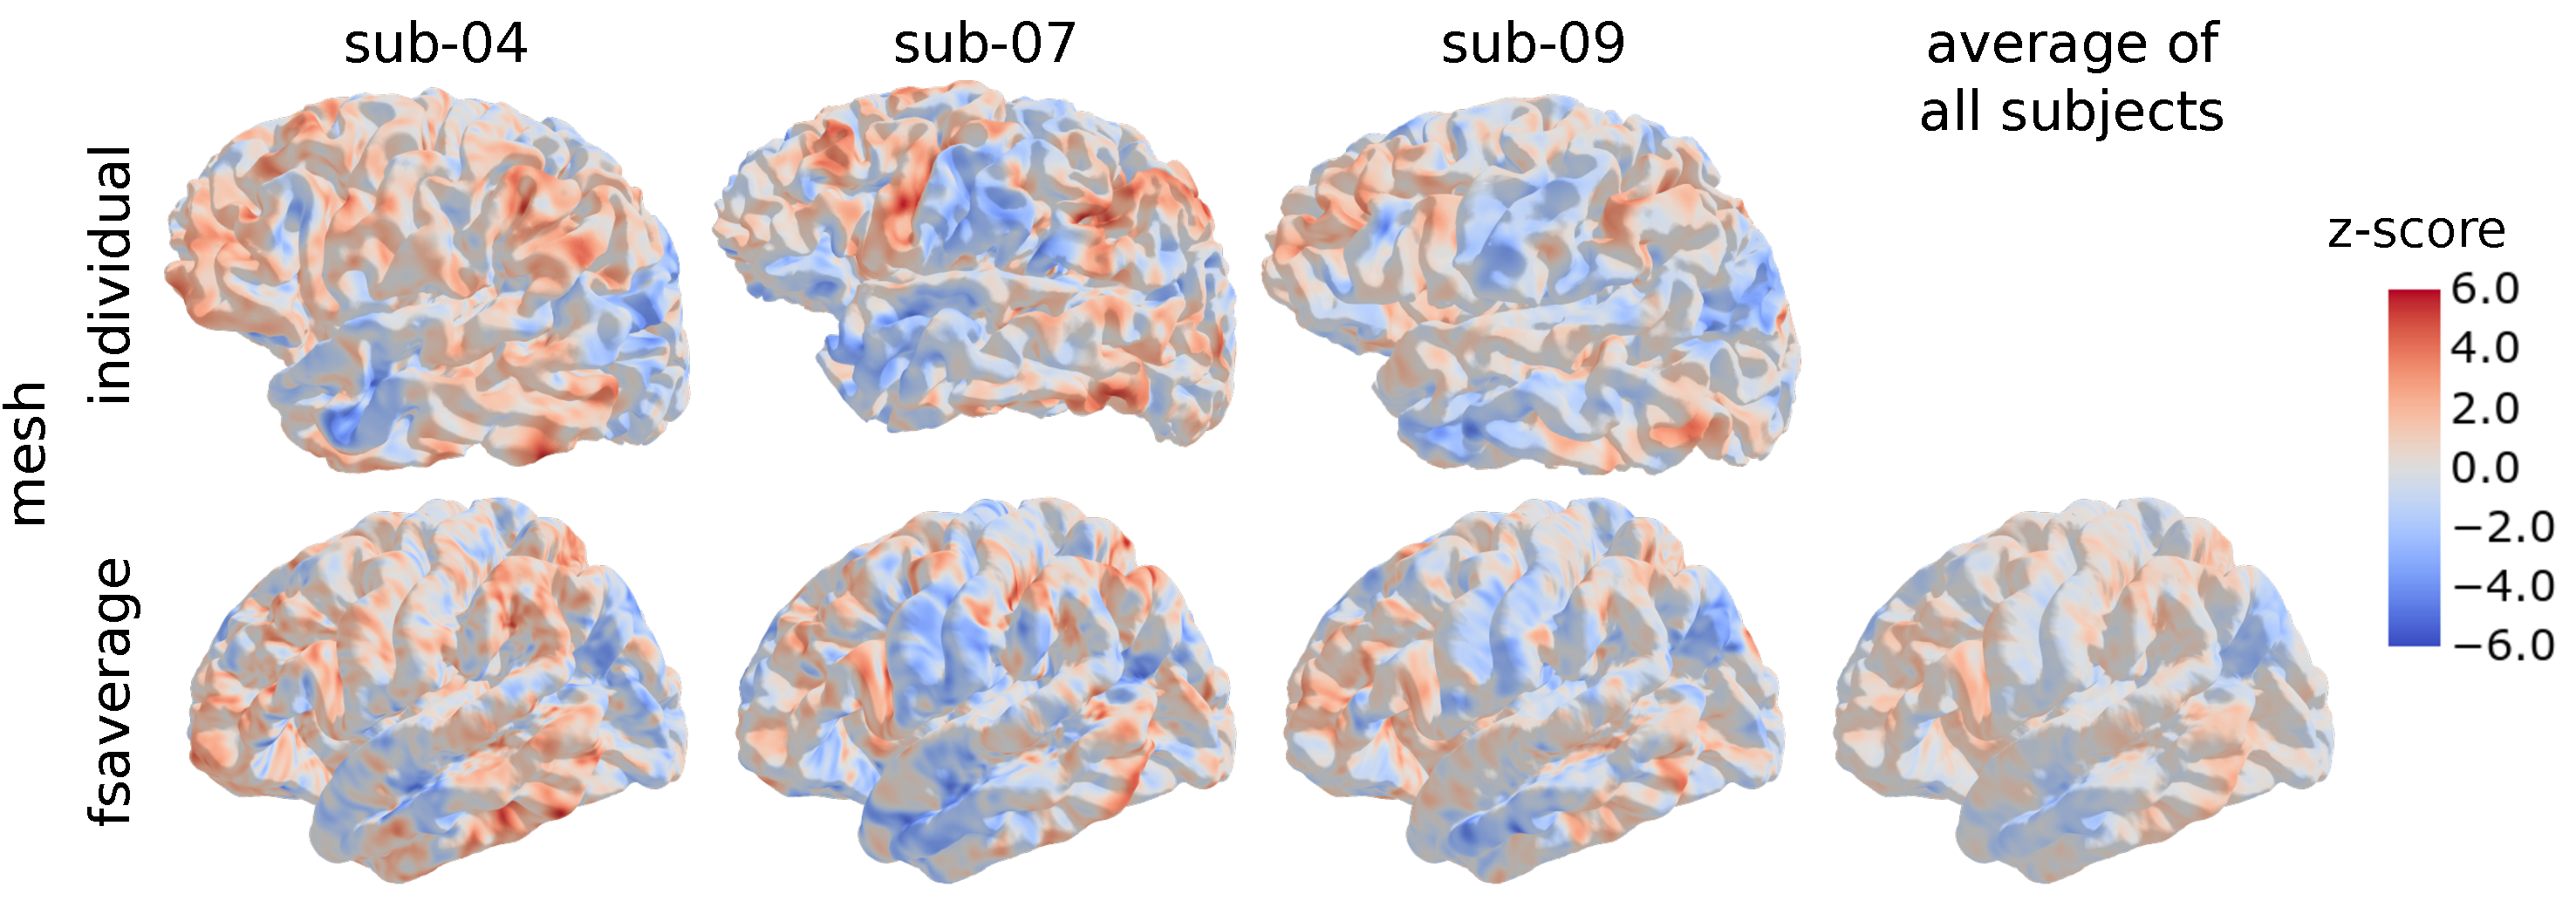
\includegraphics[width=\columnwidth]{./Chapitre4/figures/intro_variation.pdf}
    \caption{
        \textbf{High variability in human anatomies and functional MRI responses across subjects}
        In this experiment contrasting areas of the brain
        which respond to mathematical tasks against other that
        don't, we observe great variability in locations and strength of brain activations across subjects (row 1).
        The classical approach consists in wrapping this data
        to a common surface template (row 2), where they can be averaged, often resulting in
        loss of individual details and detection power.
        These images were generated using Nilearn software \citep{abraham_machine_2014}.
    }
    \label{fig:intro}
\end{figure}
In order to improve upon the current situation, a number of challenges have to be addressed:
%
\textit{(i)} There exists no template brain with functional information,
which by construction renders any cortical matching method blind to function.
This is unfortunate, since functional information is arguably the most accessible marker
to identify cortical regions and their boundaries \citep{Glasser2016-ha}.
%
\textit{(ii)} When comparing two brains -- coming from individuals or from a template --
it is unclear what regularity should be imposed on the matching \citep{vanessen2012}.
While it is traditional in medical imaging to impose diffeomorphicity \citep{ants},
such a constrain does not match the frequent observation that brain regions vary
across individuals in their fine-grained functional organization \citep{Glasser2016-ha,schneider2019}.
% \bt{find other ref}
%
\textit{(iii)} Beyond the problem of aligning human brains, it is an even greater challenge
to systematically compare functional brain organization in two different species,
such as humans and macaques \citep{neubert_comparison_2014,mars_whole_2018,xu_cross-species_2020,eichert_cross-species_2020,}.
Such inter-species comparisons intro9duce a more extreme form of variability in the correspondence model.

\paragraph{Related work}
%
Several attempts have been made to constrain the brain alignment process by using
functional information. The first one consists in introducing functional maps into
the diffeomorphic framework and search for a smooth transformation that matches
functional information \citep{sabuncu_function-based_2010,yeo_spherical_2010,robinson_msm_2014},
the most popular framework being arguably Multimodal Surface Matching (MSM)
\citep{robinson_msm_2014,Glasser2016-ha}.

A second family of less constrained functional alignment approaches have been proposed,
based on heuristics, by matching information in small, possibly overlapping,
cortical patches \citep{haxby_common_2011,Tavor2016-rl,bazeille_empirical_2021}.
%
This popular framework has been called \emph{hyperalignment}
\citep{haxby_common_2011,guntupalli_model_2016}, or \emph{shared response models} \citep{Chen2015}.
%
Yet these approaches lack a principled framework and cannot be considered to solve
the matching problem at scale. Neither do they allow to estimate %
a group-level template properly \citep{alwasity2020}.

An alternative functional alignment framework has followed another path \citep{gramfort2015},
considering functional signal as a three-dimensional distribution, and minimizing the transport cost.
However, this framework imposes unnatural constraints of non-negativity of the signal and % approximate normalization.
only works for one-dimensional contrasts, so that it cannot be used to learn
multi-dimensional anatomo-functional structures.
%
An important limitation of the latter two families of methods is that they operate on
a fixed spatial context (mesh or voxel grid), and thus cannot be used on heterogeneous meshes
such as between two individual human anatomies or, worse, between a monkey brain
and a human brain.


\paragraph{Contributions}

Following \citep{bazeille_local_2019}, we use the Wasserstein distance between source and
target functional signals -- consisting of contrast maps acquired with fMRI --
to compute brain alignments. We contribute two notable extensions of this framework:
\textit{(i)} a Gromov-Wasserstein (GW) term to preserve global anatomical structure --
this term introduces an anatomical penalization against improbably distant anatomical matches,
yet without imposing diffeomorphic regularity -- as well as
\textit{(ii)} an unbalanced correspondence that allows mappings from one brain to another
to be incomplete, for instance because some functional areas are larger in some individuals
than in others, or may simply be absent. We show that this approach successfully addresses
the challenging case of different cortical meshes, and that derived brain activity templates
are sharper than those obtained with standard anatomical alignment approaches.

\subsection{Methods}
\label{sec:methods}

Optimal Transport yields a natural framework to address the alignment problem,
as it seeks to derive a plan -- a \textit{coupling} -- that can be seen as a soft assignment matrix
between cortical areas of a source and target individual.
As discussed previously, there is a need for a functional alignment method that respects
the rich geometric structure of the anatomical features, hence the Wasserstein distance alone
is not sufficient.
By construction, the GW distance \citep{Memoli11,Memoli07}
can help preserve the global geometry underlying the signal.
The more recent fused GW distance \citep{Vayer19b} goes one step further by
making it possible to integrate functional data simultaneously with anatomical information.

\subsubsection{Fused Unbalanced Gromov-Wasserstein}

We leverage \citep{Vayer19b,Sejourne20} to present a new objective function which interpolates
between a loss preserving the global geometry of the underlying mesh structure and
a loss aligning source and target features, while simultaneously allowing not to transport
some parts of the source and target distributions. We provide an open-source solver
that minimizes this loss
\footnote{\href{https://github.com/alexisthual/fugw}{https://github.com/alexisthual/fugw}
provides a PyTorch \citep{NEURIPS2019_9015} solver with a scikit-learn \citep{scikit-learn}
compatible API}.

\paragraph{Formulation}
We denote $F^s \in \bbR^{n \times c}$ the matrix of features per vertex for the source subject.
In the proposed application, they correspond to $c$ functional activation maps,
sampled on a mesh with $n$ vertices representing the source subject's cortical surface.
Let $D^s \in \bbR^{n \times n}_+$ be the matrix of pairwise geodesic distances
\footnote{We compute geodesic distances using
\href{https://github.com/the-virtual-brain/tvb-gdist}{https://github.com/the-virtual-brain/tvb-gdist}}
between vertices of the source mesh.
Moreover, we assign the distribution $w^s \in \bbR^{n}_+$ on the source vertices.
Comparably, we define $F^t \in \bbR^{p \times c}$, $D^t \in \bbR^{p \times p}_+$ and
$w^t \in \bbR^{p}_+$ for the target subject, whose individual anatomy is represented
by a mesh comprising $p$ vertices.
Eventually, $w^s$ and $w^t$ set the transportable mass per vertex, which,
without prior knowledge, we choose to be uniform for the source and target vertices respectively:
$w^s \triangleq (\frac{1}{n}, ..., \frac{1}{n})$,
$w^t \triangleq (\frac{1}{p}, ..., \frac{1}{p})$.

Given a tuple of hyper-parameters $\theta \triangleq (\rho, \alpha, \varepsilon)$,
where $\rho, \varepsilon \in \bbR_+$ and $\alpha \in [0,1]$,
for any coupling $P \in \bbR^{n \times p}$,
we define the fused unbalanced Gromov-Wasserstein loss as
\begin{equation}
    \label{eq:fugw_obj_func}
    \begin{split}
        L_{\theta}(P) &=
        (1 - \alpha) \underbrace{\sum_{i,j} || F^s_i - F^t_j||_2^2 P_{ij}}_{\text{Wasserstein loss } L_{\text{W}}(P)}
        + \alpha \underbrace{\sum_{i,j,k,l} | D^s_{ik} - D^t_{jl}|^2 P_{ij} P_{kl}}_{\text{Gromov-Wasserstein loss } L_{\text{GW}}(P)} \\
        &+ \rho \underbrace{\left[ \kl(P_{\# 1} \otimes P_{\# 1} \vert w^s \otimes w^s)
        + \kl(P_{\# 2} \otimes P_{\# 2} \vert w^t \otimes w^t) \right]}_{\text{Marginal constraints } L_{\text{U}}(P)}
        + \varepsilon \underbrace{E(P)}_{\text{Entropy}}
    \end{split}
\end{equation}
where $L_{\text{W}}(P)$ matches vertices with similar features,
$L_{\text{GW}}(P)$ penalizes changes in geometry
and $L_{\text{U}}(P)$ fosters matching all parts of the source and target distributions.
Throughout this section, we refer to relaxing the hard marginal constraints of the underlying
OT problem into soft ones as \textit{unbalancing}.
Here, $P_{\# 1} \triangleq (\sum_j P_{i,j})_{0 \leq i < n}$ denotes
the first marginal distribution of $P$,
and $P_{\# 2} \triangleq (\sum_i P_{i,j})_{0 \leq j < p}$
the second marginal distribution of $P$. The notation $\otimes$ represents
the Kronecker product between two vectors or two matrices.
$\kl(\cdot|\cdot)$ denotes the Kullback Leibler divergence,
which is a typical choice to measure the discrepancy between two measures
in the context of unbalanced optimal transport \citep{Liero18}.
The last term $E(P) \triangleq \kl \big(P \otimes P | (w^s \otimes w^t) \otimes (w^s \otimes w^t)\big)$
is mainly introduced for computational purposes, as it helps accelerate
the approximation scheme of the optimisation problem. Typically,
it is used in combination with a small value of $\varepsilon$,
so that the impact of other terms is not diluted. On the other hand,
the parameters $\alpha$ and $\rho$ offer control over two other aspects of the problem:
while $\alpha$ realizes a trade-off between the impact of different features and
different geometries in the resulting alignment, $\rho$ controls the amount of
mass transported by penalizing configurations such that the marginal distributions
of the transportation plan $P$ are far from the prior weights $w^s$ and $w^t$.
This potentially helps adapting the size of areas where either the signal or the geometry
differs too much between source and target.

Eventually, we define $\cX^s \triangleq (F^s, D^s, w^s)$ and $\cX^t \triangleq (F^t, D^t, w^t)$,
and seek to derive an optimal coupling $P \in \bbR^{n \times p}$ minimizing
\begin{equation}
    \label{eq:fugw}
    \begin{split}
        \fugw(\cX^s, \cX^t)
        &\triangleq \inf_{P \geq 0} L_{\theta}(P).
    \end{split}
\end{equation}
This can be seen as a natural combination of the fused GW \citep{Vayer19b}
and the unbalanced GW \citep{Sejourne20} distances. To the best of our knowledge,
it has never been considered in the literature.


\paragraph{Toy example illustrating the unbalancing property}

As exemplified in \Cref{fig:intro}, brain responses elicited by the same stimulus
vary greatly between individuals.
\Cref{fig:toy_example} illustrates a similar yet simplified version of this problem,
where the goal is to align two different signals  supported on the same spherical meshes.
In this example, for each of the $n=p=3200$ vertices, the feature is simply a scalar.
On the source mesh, the signal is constituted of two von Mises density functions that differ
by their concentration (large and small), while on the target mesh, only the large one is present,
but at a different location.
We use the optimal coupling matrix $P$ obtained from Equation \eqref{eq:fugw} to transport
the source signal on the target mesh.
As shown in \Cref{fig:toy_example}.B, the parameter $\rho$ allows to control
the mass transferred from source to target.
When $\rho=100$, we approach the solution of the fused GW problem. Consequently,
we observe the second mode on the target when transporting the source signal.
When the mass control is weaker ($\rho=1$), the smaller blob is partly removed because
it has no counterpart in the target configuration, making the transport ill-posed.
\iffalse This corresponds to a mass destruction, as depicted on the right of the Figure,
whereas the larger blob in the target distribution is also a place of mass creation. \fi

\begin{figure}[t]
    \centering
    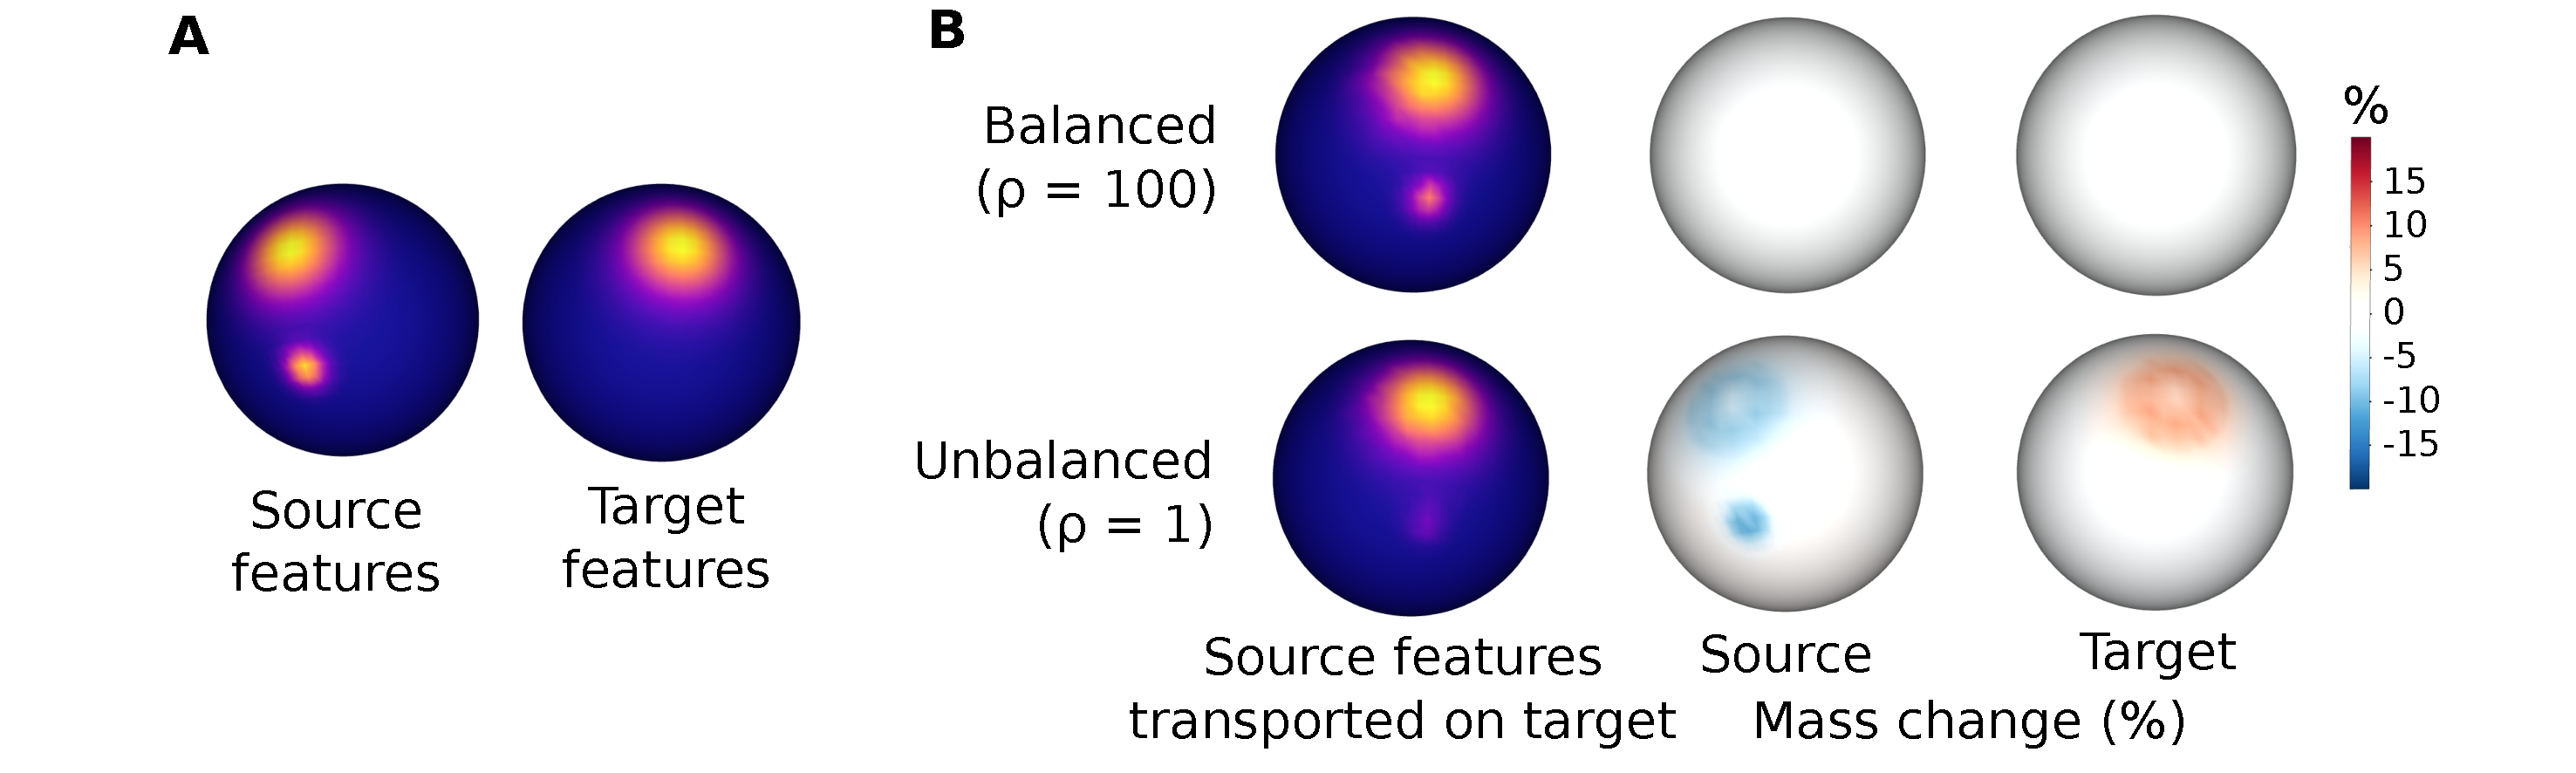
\includegraphics[width=1\columnwidth]{./Chapitre4/figures/toy_example.pdf}
    \caption{
        \textbf{Unbalancing helps accounting for idiosyncrasies of the source and target signals}
        When trying to align the source and target signals (Panel A),
        the classical balanced setup (Panel B, top row) transports all parts of
        the source signal even if they have no counterpart in the target signal.
        In the unbalanced setup (Panel B, bottom row), less source-only signal is transported:
        in particular, less mass is transported from the source's small blob onto the target
        (Panel B, middle column).
    }
    \label{fig:toy_example}
\end{figure}

%%%%%%%%%%%%%%%%%%%%%%%%%%%%%%%%%%%%%%%%%%
\subsubsection{Optimization}

Estimating the unbalanced Gromov Wasserstein loss is numerically sensitive to initialization,
due to the non-convexity of the problem.
Therefore, FUGW is also \textit{a priori} non-convex, and comparably difficult to estimate.
Consequently, following \citep{Sejourne20}, we instead compute a lower bound which
is formulated as a bi-convex problem that relies on the joint estimation of two couplings.
\begin{align}
    \label{eq:lbfugw}
    \quad \fugw(\cX^s, \cX^t) = \inf_{\substack{P, Q \geq 0 \\ P = Q}} L_{\theta}(P, Q)
    \geq \inf_{\substack{P, Q \geq 0 \\ m(P) = m(Q)}}
    L_{\theta}(P, Q) \triangleq \text{LB-FUGW} (\cX^s, \cX^t),
\end{align}
where $m(P) = \sum_{i,j} P_{i,j}$ denotes the mass of $P$ and
\begin{equation}
    \label{eq:fugw_loss_two_couplings}
    \begin{split}
        L_{\theta}(P, Q) \triangleq
        (1 - \alpha) \enspace L_{\text{W}}(P, Q) + \alpha \enspace L_{\text{GW}}(P, Q)
        + \rho \enspace L_{\text{U}}(P, Q) + \varepsilon \enspace E(P, Q),
    \end{split}
\end{equation}
where
\begin{itemize}
    \item[$\bullet$] $C \triangleq \Big( ||F^s_{i} - F^t_j||^2_2\Big)_{i,j} \in \bbR^2_+$ \hfill (feature cost matrix)

    \item[$\bullet$] $G \triangleq \Big( |D^s_{i,j} - D^t_{k,l}| \Big)_{i,j,k,l} \in \bbR^4_+$ \hfill (geometry cost matrix)

    \item[$\bullet$] $L_{\text{W}}(P, Q) \triangleq \langle C, \frac{P + Q}{2} \rangle = \frac{1}{2} ( \sum_{i,j} C_{i,j}P_{i,j} + \sum_{i,j} C_{i,j}Q_{i,j})$ \hfill (Wasserstein)

    \item[$\bullet$] $L_{\gw}(P, Q) \triangleq \langle G , P \otimes Q \rangle = \sum_{i,j,k,l}G_{i,j,k,l}P_{i,j}Q_{k,l}$ \hfill (Gromov-Wasserstein)

    \item[$\bullet$] $L_{\text{U}}(P, Q) \triangleq \enspace \kl \Big(P_{\# 1} \otimes Q_{\# 1} \vert w^s \otimes w^s \Big) + \enspace \kl \Big(P_{\# 2} \otimes Q_{\# 2} \vert w^t \otimes w^t \Big)$ \hfill (unbalancing)

    \item[$\bullet$] $E(P, Q) \triangleq \kl \Big(P \otimes Q | (w^s \otimes w^t) \otimes (w^s \otimes w^t) \Big)$ \hfill (entropy)
\end{itemize}
In particular, we have $L_{\theta}(P, P) = L_{\theta}(P)$,
which is the objective function of FUGW introduced in Equation \eqref{eq:fugw_obj_func}.
It is difficult to study when equality holds between FUGW and its lower bound.
Here, we attempt to understand the potential gap between them.
First, let us introduce the following problem
\begin{equation}
  \widetilde{\fugw}(\cX^s, \cX^t) = \inf_{(P, Q) \in \cE} L_{\theta}(P, Q),
\end{equation}
where $\cE = \{P, Q \geq 0: P_{\#1} = Q_{\#1}, P_{\#2} = Q_{\#2} \}$ is
the set of pairs of transportation plans whose corresponding marginal distributions are equal.
Clearly, we have
\begin{equation}
    \text{LB-FUGW} (\cX^s, \cX^t) \leq \widetilde{\fugw}(\cX^s, \cX^t)
    \leq \fugw(\cX^s, \cX^t).
\end{equation}
This inequality indicates that the difference between FUGW and LB-FUGW might be potentially large.
However, this gap can be tightened under the conditions in \Cref{prop:coot_gw_equiv}.
%%%%%%%%%%%%%%%%%%%%%%%%%%%%%%%%%%%%%%%%%%%%%
\begin{corollary} \label{coro:ugw_ucoot}
    If the distances $D^s$ and $D^t$ are of the forms: $D^s_{ij} = f_i + f_j + A_{ij}$ and
    $D^t_{kl} = g_k + g_l + B_{kl}$, where $f, g$ are vectors in $\bbR^n, \bbR^p$, respectively,
    and the matrices $A, B$ are both conditionally negative semi-definite, then we have
    $\fugw (\cX^s, \cX^t) = \widetilde{\fugw}(\cX^s, \cX^t)$.
    % Furthermore, if the definiteness holds, then the optimal solution satisfies $P^* = Q^*$,
    % meaning that $\text{LB-FUGW} (\cX^s, \cX^t) = \fugw(\cX^s, \cX^t)$.
\end{corollary}
%%%%%%%%%%%%%%%%%%%%%%%%%%%%%%%%%%%%%%%%%%%%%%%%
% In our experiments, while the geodesic distances do not necessarily meet these conditions,
In our experiments, while the geodesic distances do not necessarily meet these conditions,
we still observe that the two couplings of LB-FUGW are numerically equal.
So it is enough to choose, for example, the first one, as alignment between source and target signals.

The lower bound of FUGW involves solving a minimization problem with respect to two independent couplings:
Using a Block-Coordinate Descent (BCD) scheme, we fix a coupling and minimize
with respect to the other. This allows us to always be dealing with linear problems
instead of a quadratic one. Eventually, each BCD iteration consists in alternatively solving
two entropic unbalanced OT problems, whose solutions can be approximated using
the Sinkhorn algorithm \citep{Sejourne19}.

%%%%%%%%%%%%%%%%%%%%%%%%%%%%%%
\subsubsection{Barycenters}
Barycenters represent common patterns across samples.
Their role is instrumental in identifying a unique target for aligning a given group of individuals.
As seen in \Cref{fig:intro}, the vertex-wise group average does not usually provide
well-contrasted maps.
Inspired by the success of the GW distance when estimating the barycenter of structured objects
\citep{Peyre16,Vayer19b}, we use FUGW to find the barycenter
$(F_B, D_B) \in \bbR^{k \times c} \times \bbR^{k \times k}$
of all subjects $s \in \cS$, as well as the corresponding couplings $P^{s,B}$ from each subject
to the barycenter. More precisely, we solve
\begin{equation}
    \label{eq:barycenter}
    \cX^B = (F_B, D_B, w^B) \in \arg\min_{\cX}  \sum_{s \in \cS} \fugw(\cX^s, \cX),
\end{equation}
where we set the weights $w_B$ to be the uniform distribution.
By construction, the resulting barycenter benefits from the advantages of FUGW,
i.e. equilibrium between geometry-preserving and feature-matching properties,
while not forcing hard marginal constraints. The FUGW barycenter is estimated
using a Block-Coordinate Descent (BCD) algorithm that consists in alternatively
\textit{(i)} minimizing the OT plans $P^{s,B}$ for each FUGW computation
in \eqref{eq:barycenter} with fixed $\cX^B$ and \textit{(ii)}
updating the barycenter $\cX^B$ through a closed form with fixed $P^{s,B}$.
See \Cref{alg:fugw_barycenter} for more details.
The first step simply uses the previously introduced solver.
The second one takes advantage of the fact that the objective function introduced
in \eqref{eq:lbfugw} is differentiable in $F^B$ and $D^B$, and the two couplings of
LB-FUGW are numerically equal. This yields a closed form for $F^B$ and $D^B$,
as a function of $P^{s,B}$ and $\cX^s$. We note that, during the barycenter estimation,
the weight $w^B$ is always fixed as uniform distribution.

\begin{algorithm}[t]
    \caption{LB-FUGW barycenter for Problem \eqref{eq:barycenter}}
    \label{alg:fugw_barycenter}
    \begin{algorithmic}[1]
        \STATE \textbf{Input:} $(\cX^s)_{s \in \cS}, \rho, \alpha, \varepsilon$.
        \STATE \textbf{Output:} Individual couplings $(P^{s, B})_{s \in \cS}$, barycenter $\cX^B$.
        \STATE Initialize: $F^B = \mathbb I_k$; $D^B = 0_k$.
        \WHILE{$\cX^B = (F^B, D^B, w^B)$ has not converged}
            \STATE Draw $\widetilde{S}$ subset of $S$.
            \FOR{$s \in \widetilde{S}$}
                \STATE Align: $P^{s, B} \gets \text{LB-FUGW}(\cX^s, \cX^B, \rho, \alpha, \varepsilon)$.
                \COMMENT{Fixed $\cX^B$}
            \ENDFOR
            \STATE Update $F^B$, $D^B$:
            \COMMENT{Fixed $P^{s, B}$}
            \begin{equation*}
                F^B = \frac{1}{| \widetilde{S} |} \sum_{s \in \widetilde{S}}
                \text{diag} \left( \frac{1}{P^{s, B}_{\# 2}} \right)
                (P^{s, B})^\top F^s \; \text{ and } \;
                D_B = \frac{1}{| \widetilde{S} |} \sum_{s \in \widetilde{S}}
                \frac{(P^{s, B})^\top D^s P^{s, B}}{P^{s, B}_{\# 2} (P^{s, B}_{\# 2})^\top}.
            \end{equation*}
        \ENDWHILE
    \end{algorithmic}
\end{algorithm}

%%%%%%%%%%%%%%%%%%%%%%%%%%%%%%%%%%%%%%%%%ù
\subsection{Numerical experiments}

We design three experiments to assess the performance of FUGW.
In Experiments 1 and 2, we are interested in assessing if aligning pairs of individuals with
FUGW increases correlation between subjects compared to a baseline correlation.
We also compare the ensuing gains with those obtained when using the
competing method MSM \citep{robinson_msm_2014,robinson_multimodal_2018} to align subjects.
In Experiment 3, we derive a barycenter of individuals and assess its ability to capture fine-grained
details compared to classical methods.

\paragraph{Dataset}
\label{par:dataset}
In all three experiments, we leverage data from the Individual Brain Charting dataset \citep{ibc}.
It is a longitudinal study on 12 human subjects,
comprising 400 fMRI maps per subject collected
on a wide variety of stimuli (motor, visual, auditory, theory of mind,
language, mathematics, emotions, and more), movie-watching data, T1-weighted maps, as well as other features such as
retinotopy which we don't use in this work. We leverage these 400 fMRI maps.
The training, validation and test sets respectively comprise
326, 43 and 30 contrast maps acquired for each individual of the dataset.
Tasks and MRI sessions differ between each of the sets.
% More details, including preprocessing, are provided in Supplementary Materials.

\paragraph{Baseline alignment correlation}
For each pair of individuals $(s, t)$ under study, and for each fMRI contrast $c$ in the test set,
we compute the Pearson correlation $\text{corr}(F^s_{\cdot, c}, F^t_{\cdot, c})$
after these maps have been projected onto a common surface anatomy (in this case, \emph{fsaverage5}
mesh). Throughout this work, such computations are made for each hemisphere separately.

\paragraph{Experiment 1 - Aligning pairs of humans with the same anatomy}
%
For each pair $(s, t)$ under study, we derive an alignment $P^{s,t} \in \bbR^{n \times p}$
using FUGW on a set of training features. In this experiment, source and target data
lie on the same anatomical mesh (\emph{fsaverage5}), and $n = p = 10240$ for each hemisphere.
Since each hemisphere's mesh is connected, we align one hemisphere at a time.

Computed couplings are used to align contrast maps of a the validation set from
the source subject onto the target subject. Indeed, one can define
$\phi_{s \rightarrow t} \colon X \in \bbR^{n \times q}
\mapsto \big((P^{s,t})^T X \big) \oslash P^{s,t}_{\#2} \in \bbR^{p \times q}$
where $\oslash$ represents the element-wise division. $\phi_{s \rightarrow t}$
transports any matrix of features from the source mesh to the target mesh.
We measure the Pearson correlation $\text{corr}\big( \phi_{s \rightarrow t}(F^s), F^t \big)$
between each aligned source and target maps.

We run a similar experiment for MSM and compute the correlation gain induced on a
test set by FUGW and MSM respectively.
For both models, we selected the hyper-parameters maximizing correlation gain on a validation set.
In the case of FUGW, in addition to gains in correlation, hyper-parameter selection
was influenced by three other metrics that help us assess the relevance of computed couplings:

\begin{description}
    \item[Transported mass]
    For each vertex $i$ of the source subject, we compute
    $\sum \limits_{0 \leq j < p} P^{s,t}_{i, j}$.

    \item[Vertex displacement]
    Taking advantage of the fact that the source and target anatomies are the same,
    we define $D = D^s = D^t$ and compute for each vertex $i$ of the source subject the quantity
    $\sum_j P^{s,t}_{i, j} \cdot D_{i, j} / \sum_j P^{s,t}_{i,j}$,
    which measures the average geodesic distance on the cortical sheet between vertex $i$
    and the vertices of the target it has been matched with.

    \item[Vertex spread]
    Large values of $\varepsilon$ increase the entropy of derived couplings.
    To quantify this effect, and because we don't want the matching to be too blurry,
    we assess how much a vertex was \textit{spread}. Considering
    $\tilde{P_i} = P^{s,t}_i / \sum_j P^{s,t}_{i,j} \in \bbR^p$
    as a probability measure on target vertices,
    we estimate the anatomical variance of this measure by sampling $q$ pairs
    $(j_q, k_q)$ of $\tilde{P_i}$ and computing their average geodesic distance
    $\frac{1}{q} \sum\limits_{j_q, k_q} D_{j_q, k_q}$.
\end{description}

\paragraph{Experiment 2 - Aligning pairs of humans with individual anatomies}
We perform a second alignment experiment, this time using individual meshes instead of
an anatomical template. Importantly, in this case,  there is no possibility to compare
FUGW with baseline methods, since those cannot handle this case.
However, individual meshes are significantly larger than the
common anatomical template used in Experiment 1 ($n \approx m \approx$ 160k vs. 10k previously),
resulting in couplings too large to fit on GPUs -- for reference,
a coupling of size 10k $\times$ 10k already weights ~400Mo on disk.
We thus reduce the size of the source and target data by
clustering them into 10k small connected clusters using Ward's algorithm \citep{thirion:2014}.
% More details are given in supplementary section A.4.

\paragraph{Experiment 3 - Comparing FUGW barycenters with usual group analysis}
\label{par:barycenter}

Since it is very difficult to estimate the barycentric mesh, we force it to be equal to
the \emph{fsaverage5} template. Empirically, this we force the distance matrix $D^B$
to be equal to that of \emph{fsaverage5}, and only estimate the functional barycenter $F^B$.
We initialize it with the mean of $(F^s)_{s \in S}$
and derive $F^B$ and $(P^{s,B})_{s \in S}$ from Problem \eqref{eq:barycenter}.
Then, for a given stimulus $c$, we compute its projection onto the barycenter for each subject.
We use these projections to compute two maps of interest:
\textit{(i)} $M_{B,c}$ the mean of projected contrast maps across subjects
and \textit{(ii)} $T_{B,c}$ the t-statistic (for each vertex) of projected maps.
We compare these two maps with their unaligned counterparts $M_{0,c}$ and $T_{0,c}$ respectively.
\begin{figure}[ht]
    \begin{minipage}{.4\linewidth}
        \begin{equation*}
            M_{B,c} \triangleq \frac{1}{|S|} \sum_{s \in S} \phi_{s \rightarrow t}(F^s_{\cdot, c})
        \end{equation*}
    \end{minipage}
    \hfil
    \begin{minipage}{.5\linewidth}
        \begin{equation*}
            T_{B,c} \triangleq \text{t-statistic} \Big( \big(
                \phi_{s \rightarrow t}(F^s_{\cdot, c}) \big)_{s \in S} \Big)
        \end{equation*}
    \end{minipage}
\end{figure}
% \vspace*{-0.5\baselineskip}
\begin{figure}[ht]
    \begin{minipage}{.4\linewidth}
        \begin{equation*}
            M_{0,c} \triangleq \frac{1}{|S|} \sum_{s \in S} F^s_{\cdot, c}
        \end{equation*}
    \end{minipage}
    \hfil
    \begin{minipage}{.5\linewidth}
        \begin{equation*}
            T_{0,c} \triangleq \text{t-statistic} \Big( (F^s_{\cdot, c})_{s \in S} \Big)
        \end{equation*}
    \end{minipage}
\end{figure}
The first map helps us to qualitatively evaluate the precision of FUGW alignments and barycenter.
The second one is classically used to infer the existence of areas of the brain that
respond to specific stimuli. We assess whether FUGW helps find the same clusters of vertices.
Eventually, we quantify the number of vertices significantly activated or deactivated
with and without alignment respectively.

\subsection{Results}

\subsubsection{Experiment 1 - Template anatomy}

\paragraph{Aligning subjects on a fixed mesh}

We set $\alpha = 0.5$, $\rho = 1$ and $\varepsilon = 10^{-3}$.
Pearson correlation between source and target contrast maps is systematically and
significantly increased when aligned using FUGW, as illustrated in
\Cref{fig:gain_comparisions_fsaverage5} where correlation grows by almost $40\%$
from $0.258$ to $0.356$.

\begin{figure}[ht!]
    \centering
    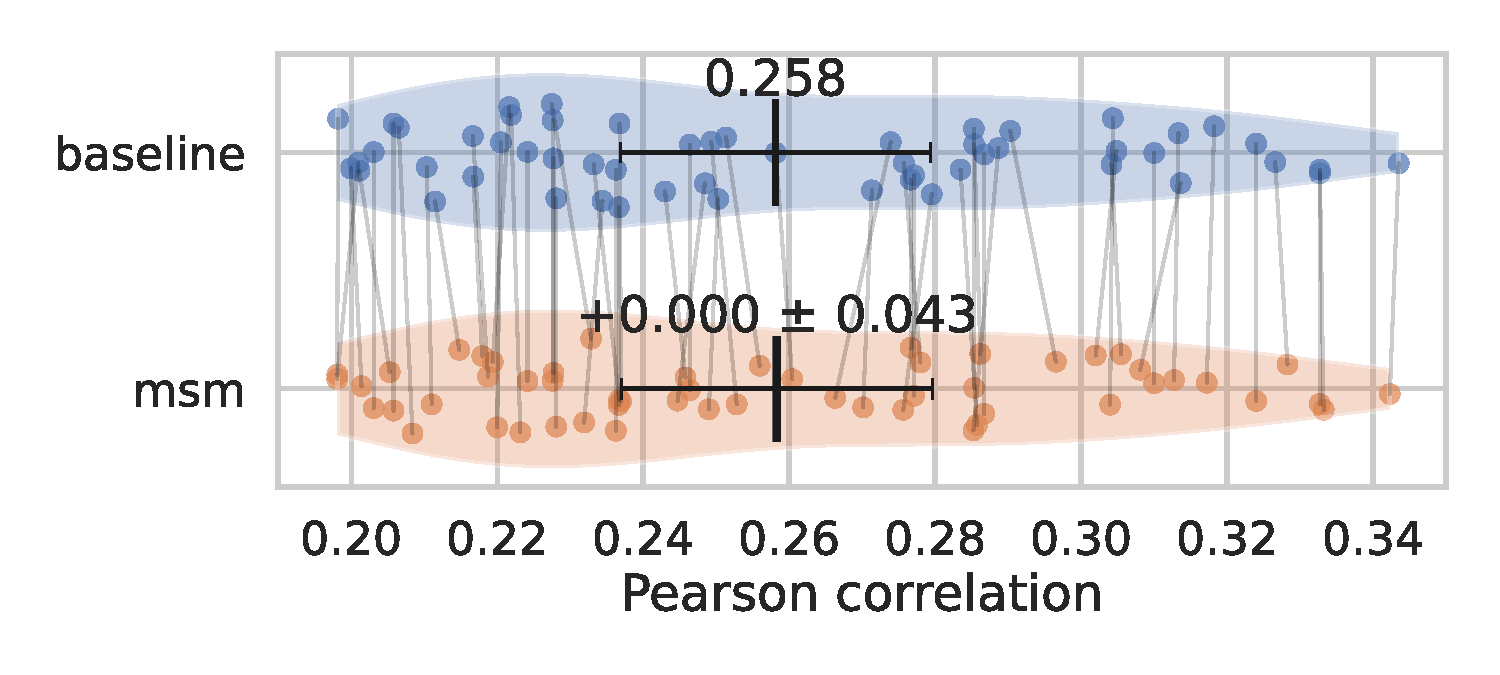
\includegraphics[width=0.49\columnwidth]{./Chapitre4/figures/fsaverage5_alignment_correlation_gain_msm.pdf}
    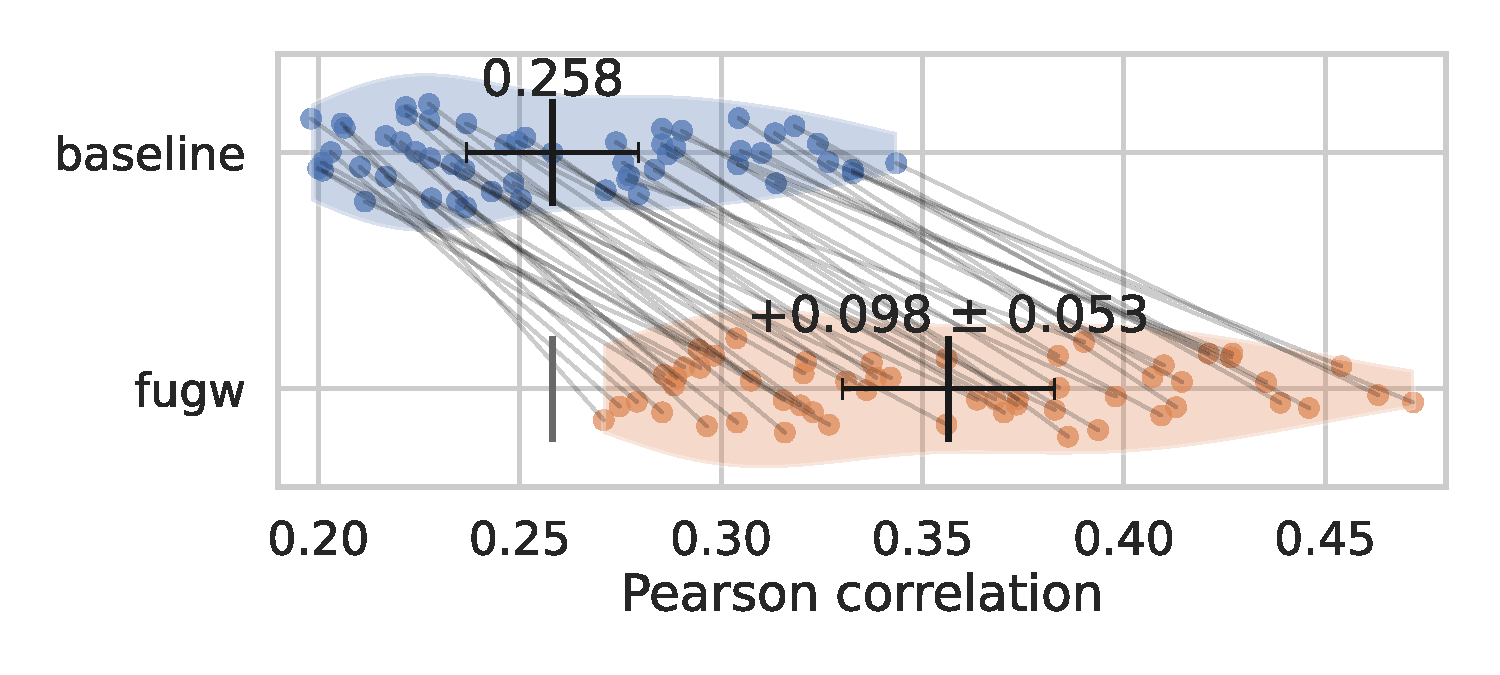
\includegraphics[width=0.49\columnwidth]{./Chapitre4/figures/fsaverage5_alignment_correlation_gain_fugw.pdf}
    \caption{
        \textbf{Comparison of gains in correlation after inter-subject alignment}
        For each pair of source and target subjects of the dataset,
        we compute the average Pearson correlation between 30 test contrasts,
        leading to the (baseline) correspondence score,
        and compare it with that of the same contrast maps
        aligned with either MSM (left) or FUGW (right). Correlation gains are much better for FUGW.
    }
    \label{fig:gain_comparisions_fsaverage5}
\end{figure}
% We also varied training sets by selecting subsets of training contrasts and find that
% similar performance on the test set can be achieved regardless of the training data
% (see Supplementary \Cref{sec:control_experiments} and in particular Supplementary
% \Cref{tab:varying_training_sets}).

\paragraph{Hyper-parameters selection}
\label{par:params_selection}

Hyper-parameters used to obtain these results were chosen
after running a grid search on $\alpha$, $\varepsilon$ and $\rho$
and evaluating it on the validation dataset.
Computation took about 100 hours using 4 Tesla V100-DGXS-32GB GPUs. More precisely,
it takes about 4 minutes to compute one coupling between a source and target 10k-vertex
hemisphere on a single GPU, when the solver was set to run 10 BCD and 400 Sinkhorn iterations.
In comparison, MSM takes about the same time on Intel(R) Xeon(R) CPU E5-2698 v4 @ 2.20GHz CPUs.
Results are reported in \Cref{fig:cv_metrics} and provide multiple insights concerning FUGW.

Firstly, without anatomical constraint ($\alpha = 0$),
source vertices can be matched with target vertices
that are arbitrarily far on the cortical sheet.
Even though this can significantly increase correlation, it also
results in very high vertex displacement values (up to $100mm$).
Such couplings are not anatomically plausible.
%
Secondly, without functional information ($\alpha = 1$),
couplings recover a nearly flawless matching between source and target meshes,
so that, when $\varepsilon = 10^{-5}$
(ie when we force couplings to find single-vertex-to-single-vertex matches),
vertex displacement and spread are close to 0 and correlation is unchanged.
%
Fusing both constraints ($0 < \alpha < 1$)
yields the largest gains in correlation while allowing to compute
anatomically plausible reorganizations the cortical sheet between subjects.

The impact of $\rho$ (controlling marginal penalizations) on correlation seems modest,
with a slight tendency of increased correlation in unbalanced problems (low $\rho$).

Finally, it is worth noting that a relatively wide range of $\alpha$ and $\rho$ yield comparable gains.
The fact that FUGW performance is weakly sensitive to hyper-parameters makes it
a good off-the-shelf tool for neuroscientists who wish to derive inter-individual alignments.
However, $\varepsilon$ is of dramatic importance in computed results and should be chosen carefully.
Vertex spread is a useful metric to choose sensible values of $\varepsilon$;
for human data one might consider that it should not exceed $20mm$.

\begin{figure}[ht]
    \centering
    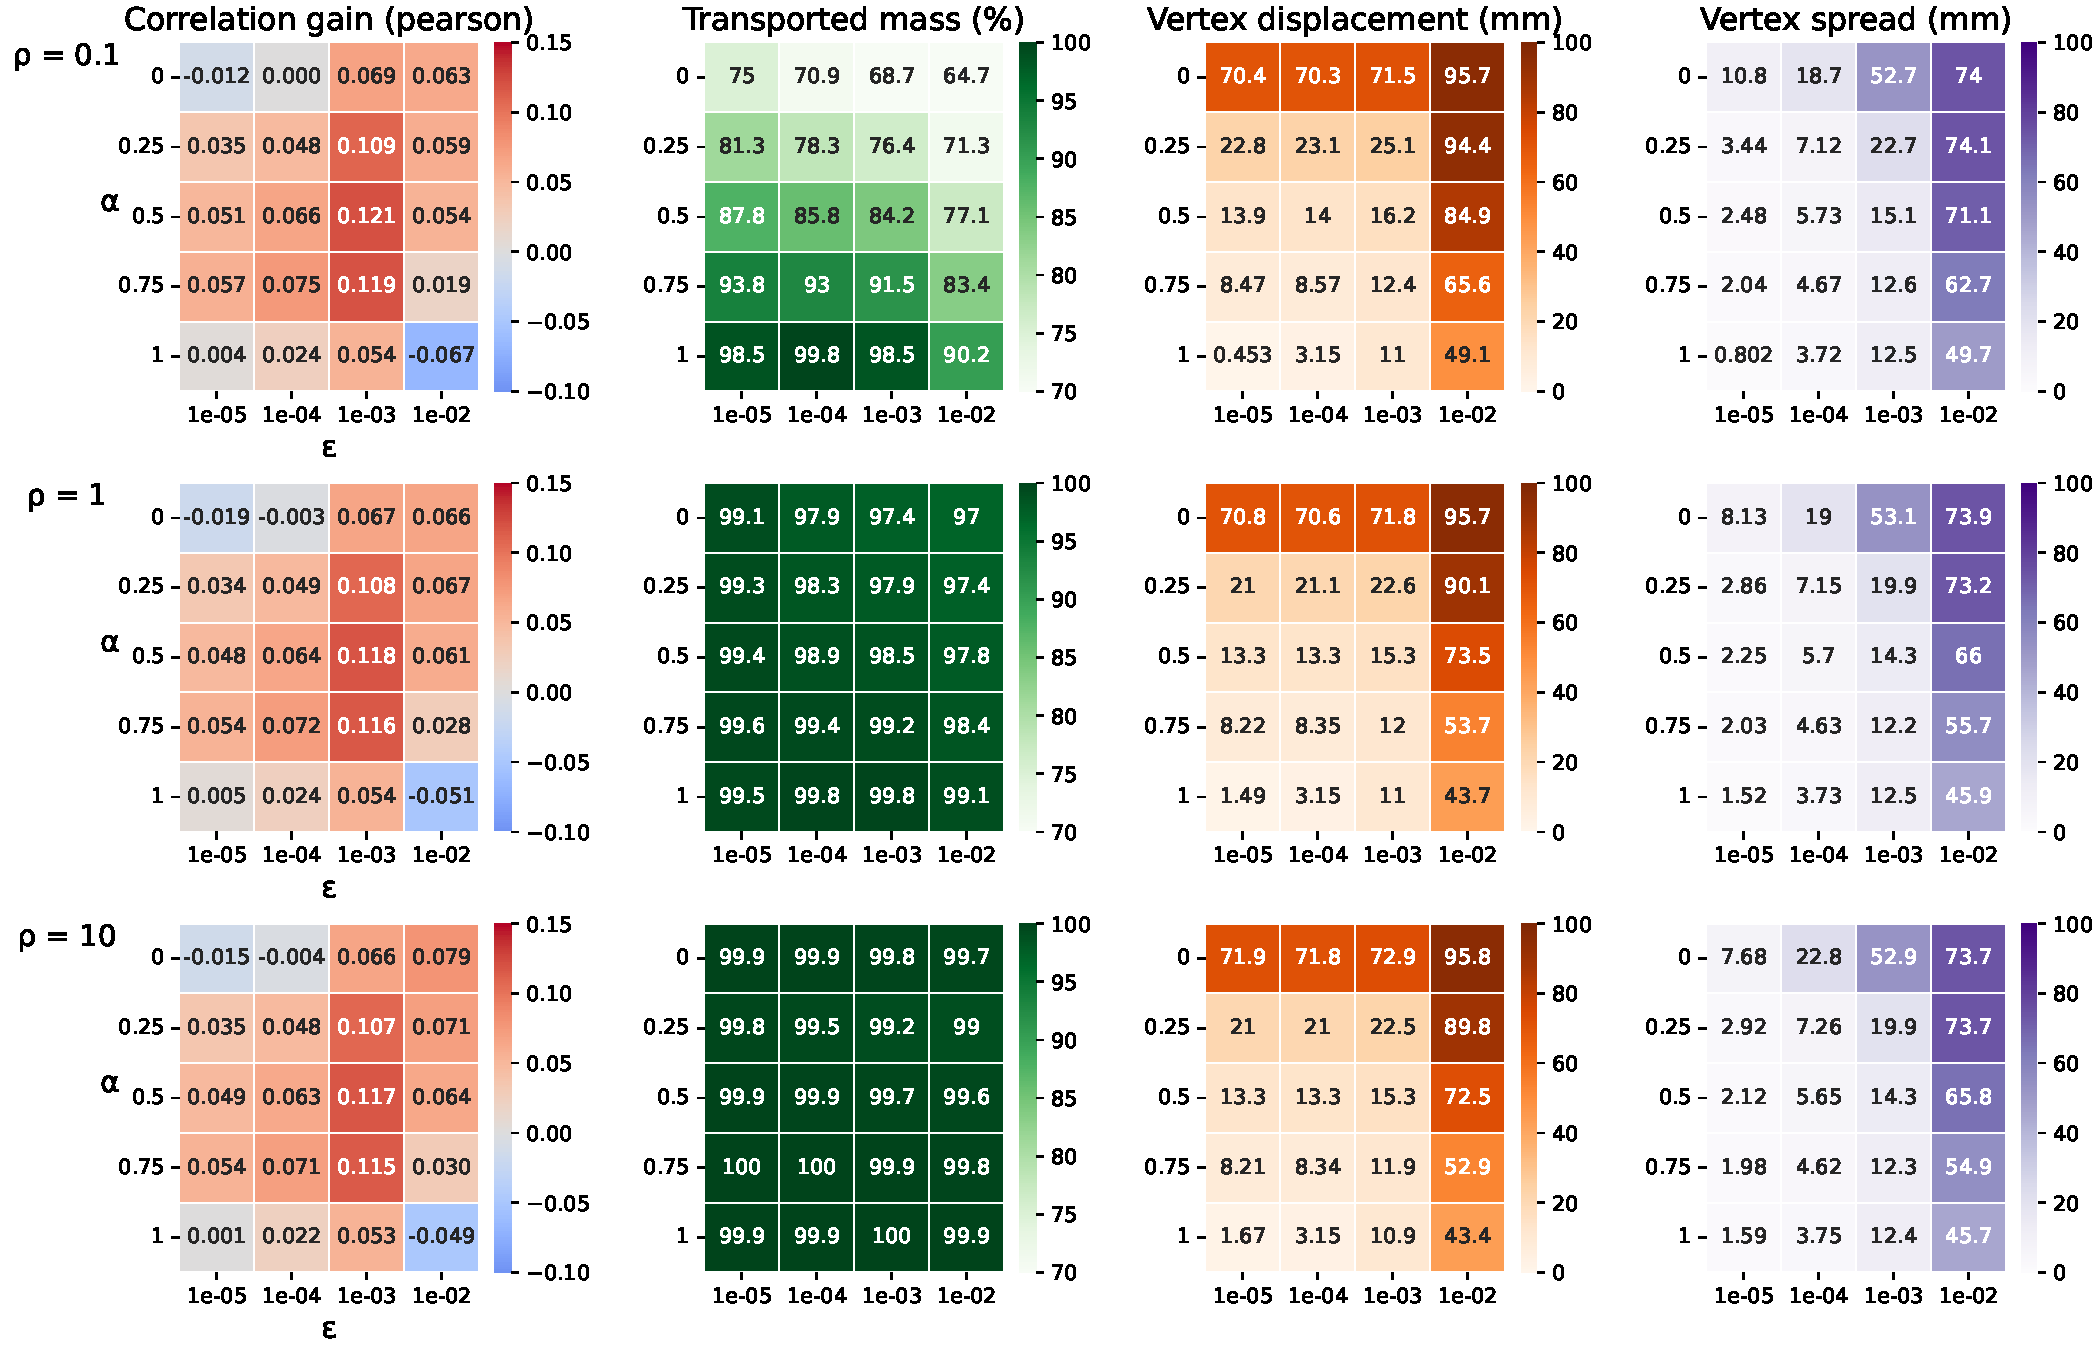
\includegraphics[width=1\columnwidth]{./Chapitre4/figures/cv_all_metrics_hcp_left_fugw.pdf}
    \caption{
        \textbf{Exploring hyper-parameter space to find relevant couplings}
        Given a transport plan aligning a source and target subject,
        we evaluate how much this coupling
        (left) improves correlation between unseen contrast maps
        of the two subjects,
        (center left) actually transports data,
        (center right) moves vertices far from their original location on the cortical surface
        and (right) spreads vertices on the cortical sheet.
        We seek plans that maximize correlation gain, while keeping spread and displacement low enough.
    }
    \label{fig:cv_metrics}
\end{figure}

\paragraph{Mass redistribution in unbalanced couplings}
Unbalanced couplings provide additional information about how functional areas might differ
in size between pairs of individuals. This is illustrated in \Cref{fig:transported_mass},
where we observe variation in size of the auditory area between a given pair of individuals.
This feature is indeed captured by the difference of mass between subjects
(although the displayed contrast was not part of the training set).
\begin{figure}[!th]
    \centering
    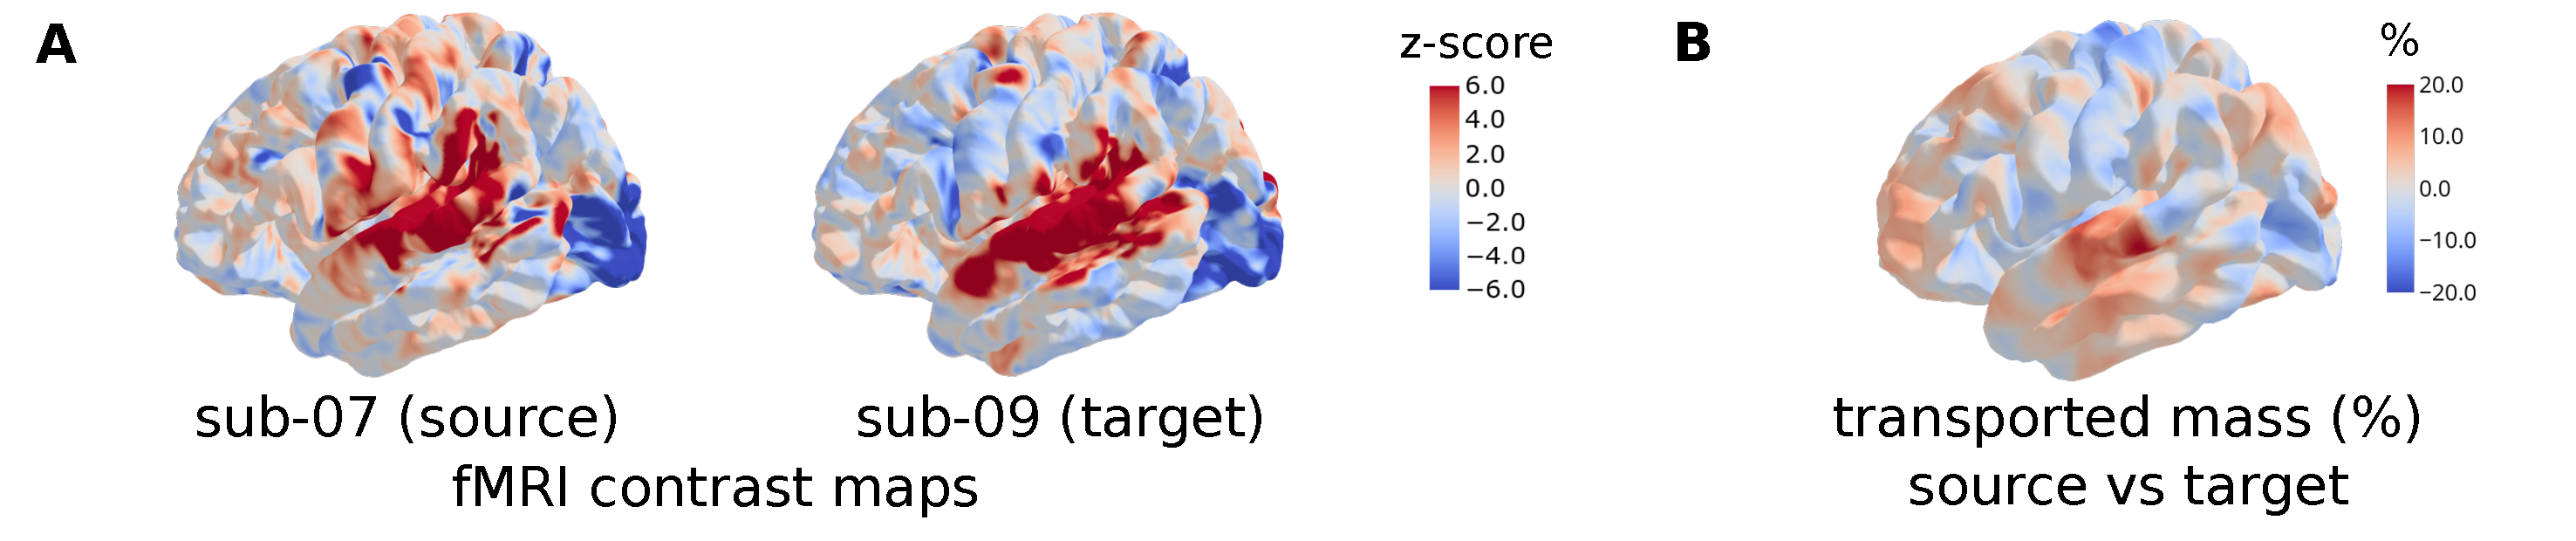
\includegraphics[width=1\columnwidth]{./Chapitre4/figures/transported_mass.pdf}
    \caption{
        \textbf{Transported mass indicates areas which have to be resized between subjects}
        (Panel A) We show a contrast map from the test set which displays areas showing
        stronger activation during auditory tasks versus equivalent visual tasks. It shows much more
        anterior activations on the target subject compared to the source subject.
        This is consistent with the observation that more mass is present in
        anterior auditory areas of the source subject than in the target subject (Panel B).
    }
    \label{fig:transported_mass}
\end{figure}

\subsubsection{Experiment 2 - Individual anatomies}
\begin{figure}[!ht]
    \centering
    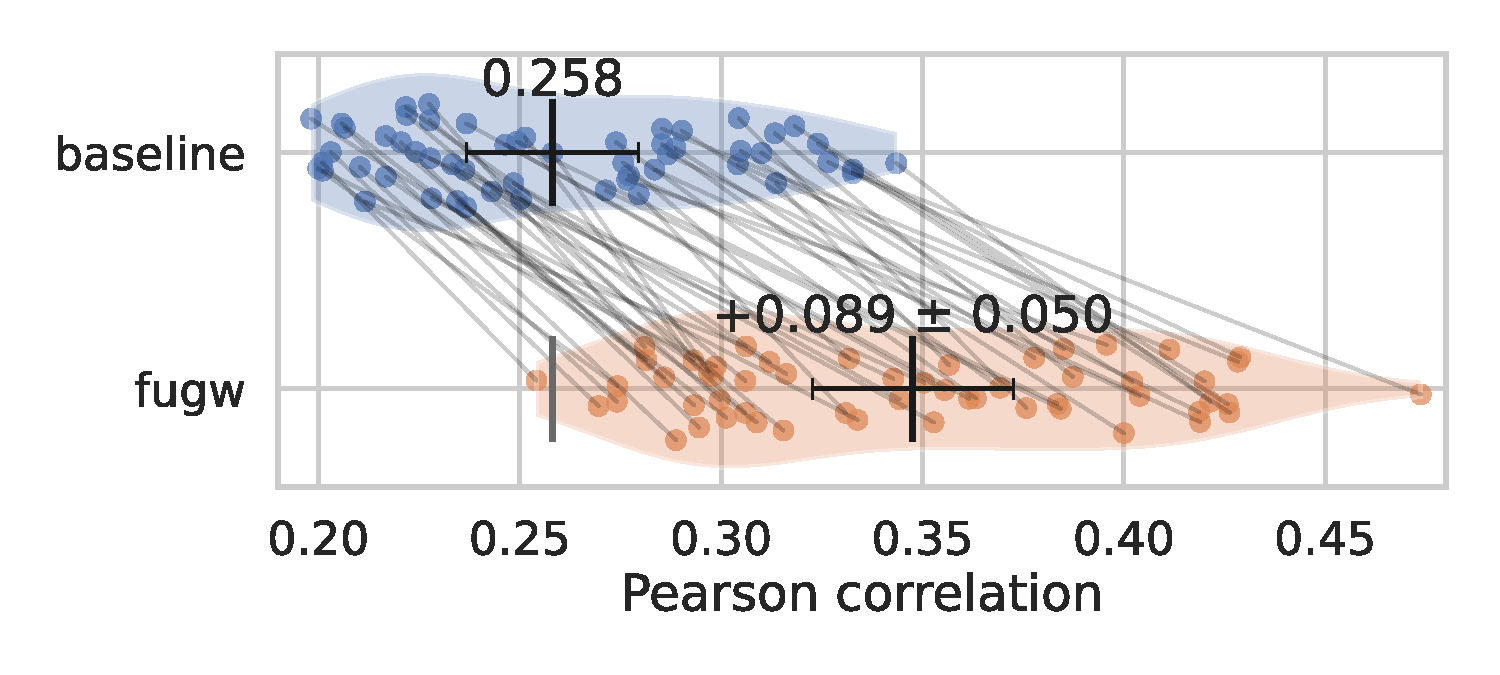
\includegraphics[width=0.5\columnwidth]{./Chapitre4/figures/individual_alignment_correlation_gain_fugw}
    \caption{
        \textbf{Correlation between pairs of subjects is significantly better after alignment on individual anatomies than after projecting subjects onto a common anatomical template}
    }
    \label{fig:gain_comparisions_individual}
\end{figure}

As shown in \Cref{fig:gain_comparisions_individual},
we obtain correlation gains which are comparable to that of Experiment 1 (about 35\% gain)
while working on individual meshes.
This tends to show that FUGW can compute meaningful alignments between pairs of individuals
without the use of an anatomical template, which helps bridge most conceptual impediments listed
in \Cref{sec:introduction}.
Moreover, this opens the way for computation of simple statistics in cohorts of individuals
in the absence of a template. Indeed, one can pick an individual of the cohort and use it
as a reference subject on which to transport all other individuals.
We give an example in \Cref{fig:individual_projections},
showing that FUGW correctly preserved idiosyncrasies of each subject while
transporting their functional signal in an anatomically sound way.
\begin{figure}[H]
    \centering
    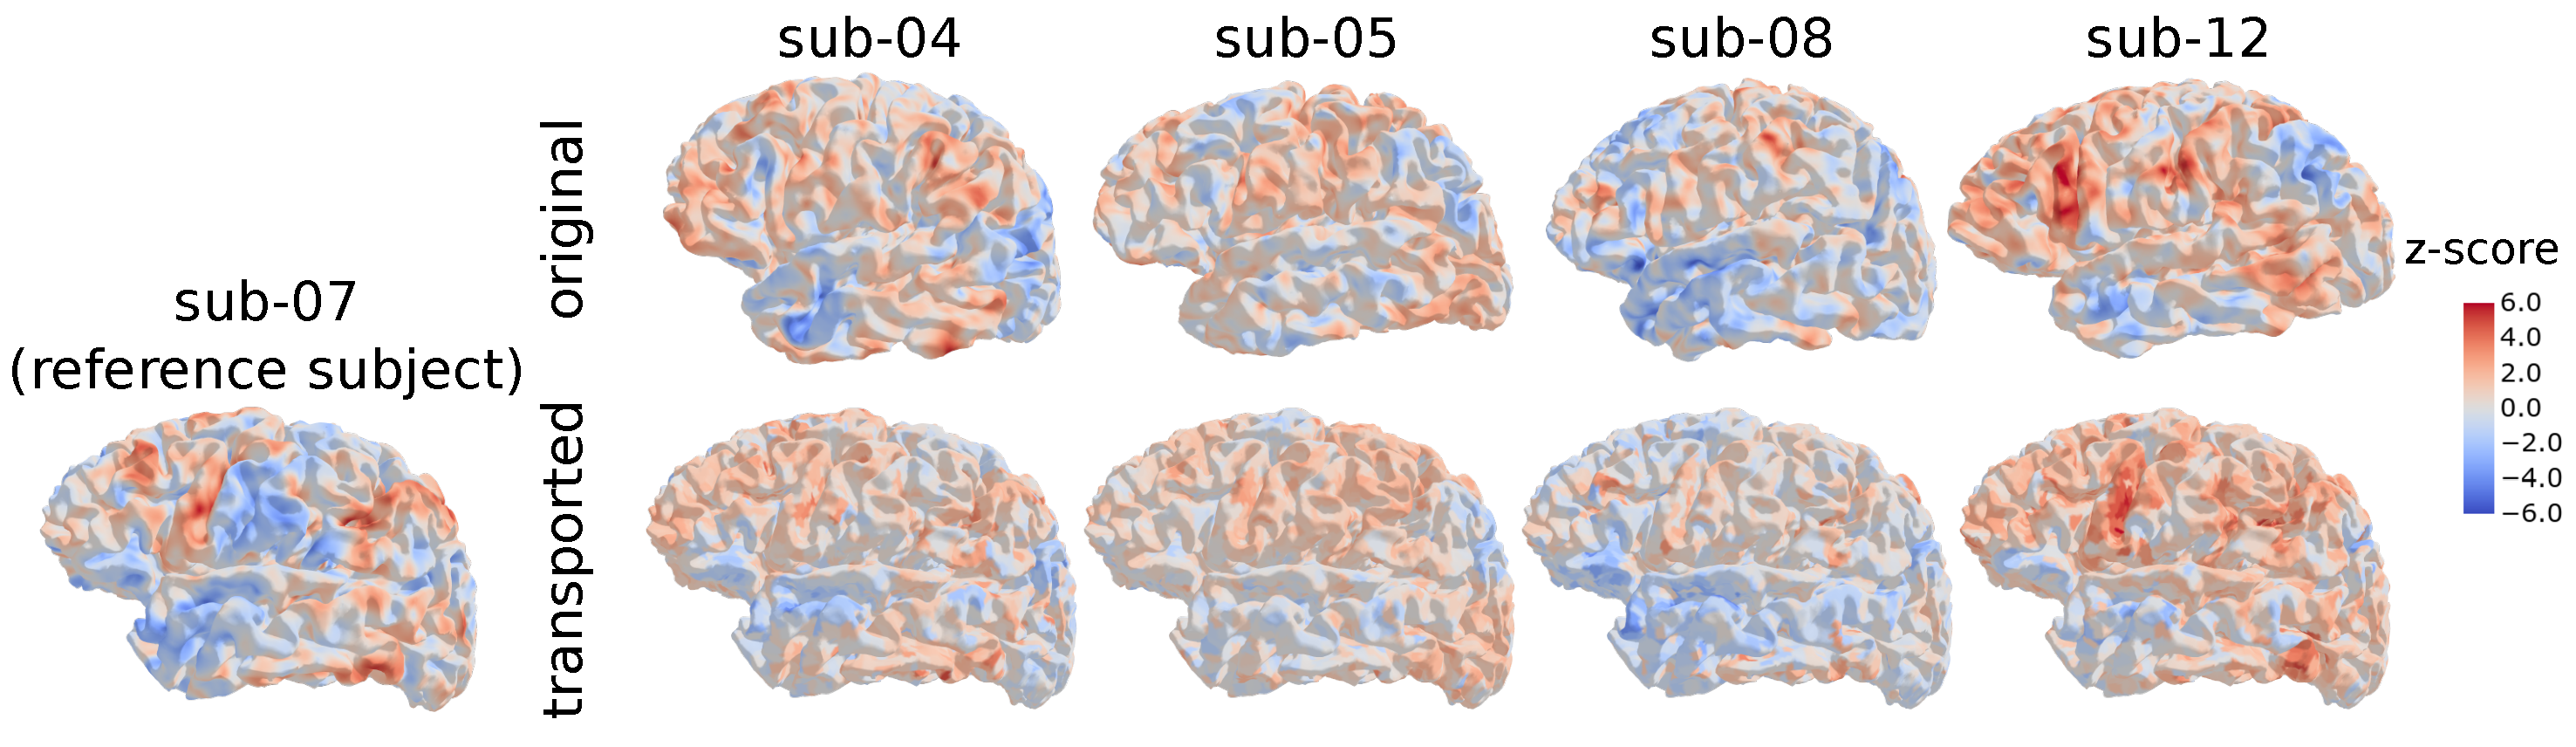
\includegraphics[width=1\columnwidth]{./Chapitre4/figures/individual_alignment.pdf}
    \caption{
        \textbf{Transporting individual maps onto a reference subject}
        FUGW can help bridge the absence of template anatomies
        and derive pairs of alignments such that all individuals
        of the cohort are comparable. We display a map taken from the test set contrasting areas activated during mathematical reasoning against areas activated for other stimuli of the protocol.
    }
    \label{fig:individual_projections}
\end{figure}

\subsubsection{Experiment 3 - Barycenter}

In the absence of a proper metric to quantify the correctness of a barycenter,
we first qualitatively compare the functional templates obtained with and without alignment.
In \Cref{fig:barycenter_vs_group_average}.A, we do so using brain maps taken from the test set.
We can see that the barycenter obtained with FUGW yields sharper contrasts and
more fine-grained details than the barycenter obtained by per-vertex averaging.
We also display in \Cref{fig:barycenter_vs_group_average}.B
the result of a one-sample test for the same contrast, which can readily be used for inference.
The one-sample test map obtained after alignment to the FUGW template exhibits
the same supra-threshold clusters as the original approach, but also some additional spots
which were likely lost due to inter-subject variability in the \emph{fsaverage5} space.
This approach is thus very useful to increase power in group inference.
We quantify this result by counting the number of supra-threshold vertices
with and without alignment for each contrast map of the test set.
Our alignment method significantly finds more such vertices of interest,
as shown in \Cref{fig:barycenter_vs_group_average}.C.
\begin{figure}[t]
    \centering
    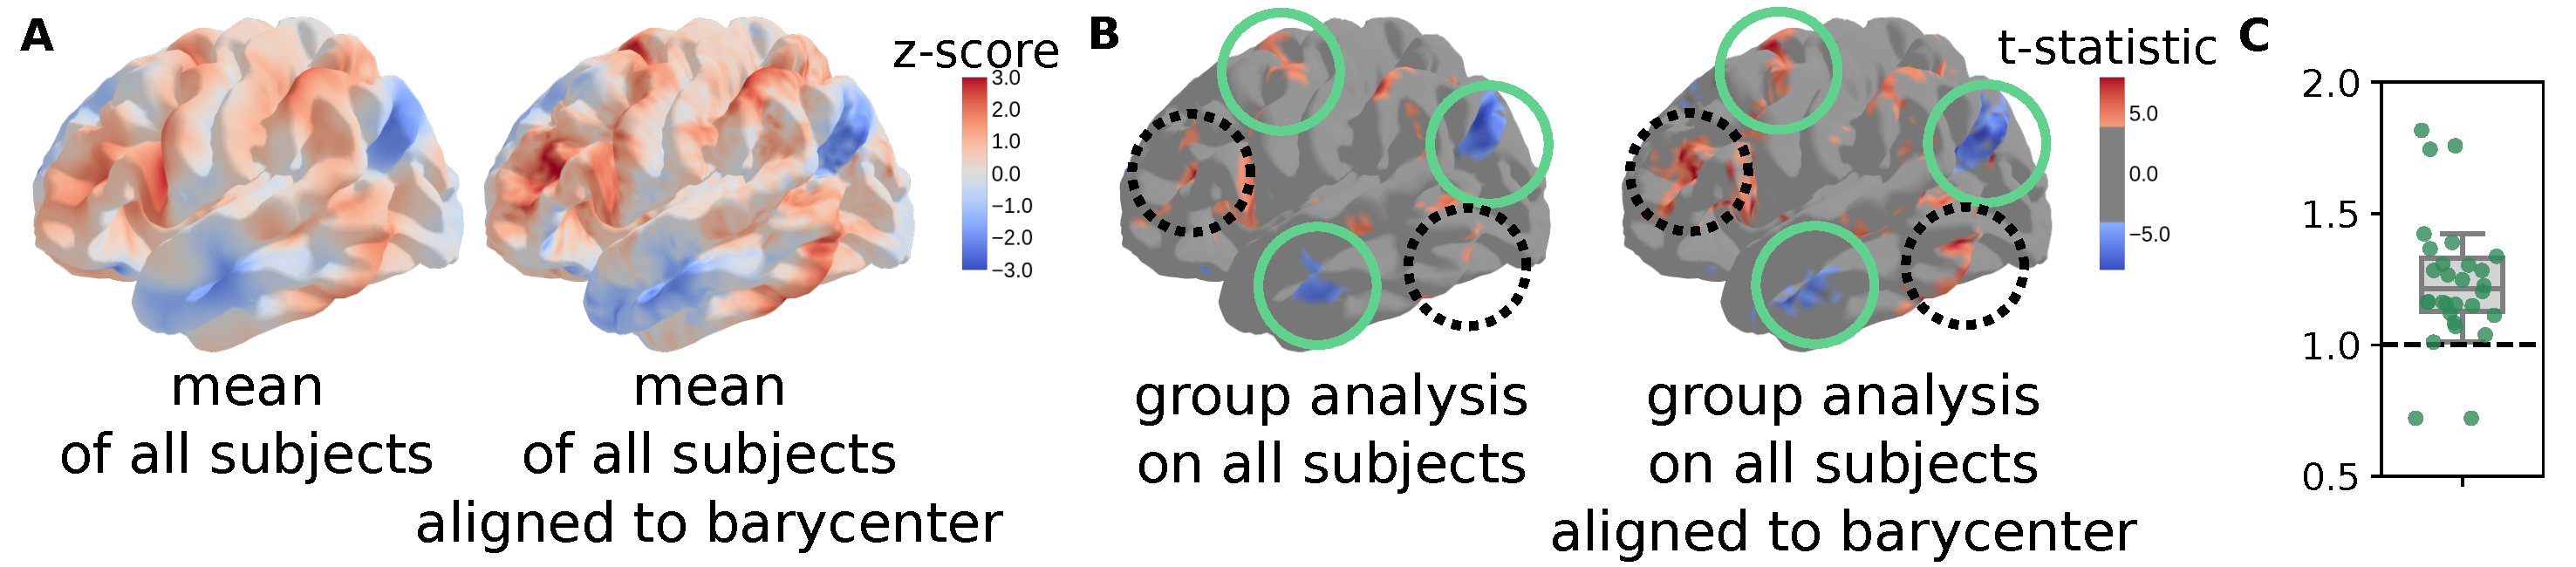
\includegraphics[width=1\columnwidth]{./Chapitre4/figures/barycenter_group_analysis.pdf}
    \caption{
        \textbf{FUGW barycenter yields much finer-grained maps than group averages}
        We study the same statistical map as in \Cref{fig:intro}, which contrasts
        areas of the brain involved in mathematical reasoning.
        \textbf{A}. These complex maps projected onto the barycenter and averaged
        show more specific activation patterns than simple group averages,
        especially in cortical areas exhibiting more variability, such as the prefrontal cortex.
        \textbf{B}. Deriving a t-test on aligned maps captures the same clusters
        as the classical approach (plain green circles), but also new clusters in areas
        where inter-subject variability is high (dotted black circles).
        Peak t-statistics are also higher with FUGW.
        \textbf{C}. Ratio of number of activated vertices ($|\text{t-statistic}| \geq 4$)
        with versus without alignment for each map of the test set.
        Our method finds significantly more of such vertices ($\text{p-value} = 3\cdot10^{-4}$).}
    \label{fig:barycenter_vs_group_average}
\end{figure}

\subsection{Discussion}

FUGW can derive meaningful couplings between pairs of subjects without
the need of a pre-existing anatomical template. It is well-suited to computing
barycenters of individuals, even for small cohorts.

In addition, we have shown clear evidence that FUGW yields gains that cannot be achieved
by traditional diffeomorphic registration methods.
These methods impose very strong constraints to the displacement field,
that may prevent reaching optimal configurations.
More deeply, this finding suggests that brain comparison ultimately requires
lifting hard regularity constraints on the alignment models,
and that two human brains differ by more than a simple continuous surface deformation.
However, current results have not shown a strong correlation gain of
unbalanced OT compared to balanced OT, likely because the cohort under study is too small.
Leveraging datasets such as HCP \citep{hcpdata} with a larger number of subjects
will help lower the standard error on correlation gain estimates.
In this work, we decided to rely on a predefined anatomical template (\emph{fsaverage5})
to derive functional barycenters.
It would be interesting to investigate whether more representative anatomical templates
can be learned during the process.
This would in particular help to customize templates to different populations or species.

Additionally, using an entropic solver introduces a new hyper-parameter $\varepsilon$
that has a strong effect, but is hard to interpret.
Future work may replace the Sinkhorn algorithm \citep{Sejourne19}
used here by the majorization-minimization one \citep{Chapel20},
which does not require entropic smoothing. This solution can yield sparse couplings
while being orders of magnitude faster, which will prove useful when computing barycenters
on large cohorts.

Finally, we plan to make use of FUGW to derive alignments between human and
non-human primates without anatomical priors. Indeed, the understanding of given brain mechanisms
will benefit from more detailed invasive measurements made on other species \emph{only if}
brains can be matched across species; moreover, this  raises the question of features
that make the human brain unique, by identifying patterns that have no counterpart in other species.
By maximizing the functional alignment between areas, but also allowing for some regions
to be massively shrunk or downright absent in one species relative to the other,
the present tool could shed an objective light on the important issue of whether
and how the language-related areas of the human cortical sheet map onto
the architecture of non-human primate brains.

\vfill

\chapter{Fused Unbalanced Gromov-Wasserstein} \label{chap:fugw}

% \addcontentsline{tot}{chapter}{section}
\renewcommand{\contentsname}{Contents}
\localtableofcontents*
\chaptermark{\textbf{Fused Unbalanced Gromov-Wasserstein}}

\hfill \break

\raggedbottom

This chapter presents the results from \citep{Thual22} and addresses the applications of
unbalanced extension of fused Gromov-Wasserstein in human brains alignments.
Individual brains vary in both anatomy and functional organization, even within a given species.
Inter-individual variability is a major impediment when trying to draw generalizable conclusions
from neuroimaging data collected on groups of subjects.
Current co-registration procedures rely on limited data, and thus lead to very coarse
inter-subject alignments.
In this work, we present a novel method for inter-subject alignment based on Optimal Transport,
denoted as Fused Unbalanced Gromov-Wasserstein (FUGW).
The method aligns cortical surfaces based on the similarity of their functional signatures in
response to a variety of stimulation settings, while penalizing large deformations of
individual topographic organization.
We demonstrate that FUGW is well-suited for whole-brain landmark-free alignment.
The unbalanced feature allows to deal with the fact that functional areas
vary in size across subjects. Our results show that FUGW alignment significantly
increases between-subject correlation of activity for independent functional data,
and leads to more precise mapping at the group level.

\raggedbottom

%%%%%%%%%%%%%%%%%%%%%%%%%%%
\section{Introduction}
\label{sec:introduction}

The availability of millimeter or sub-millimeter anatomical or functional brain images has opened
new horizons to
neuroscience, namely that of mapping cognition in the human brain and detecting markers of diseases.
%
Yet this endeavour has stumbled on the roadblock of inter-individual
variability: while the overall organization of the human brain is largely invariant,
two different brains (even from monozygotic twins \citep{pizzigali2020})
may differ at the scale of centimeters in shape, folding pattern, and functional responses.
%
% While variability is a hindrance to brain mapping,
The problem is further complicated by the fact that functional images
are noisy, due to imaging limitations and behavioral
differences across individuals that cannot be easily overcome.
%
The status quo of the field is thus to rely on anatomy-based inter-individual alignment
that approximately matches the outline of the brain \citep{ants}
as well as its large-scale cortical folding patterns \citep{fs_reconall,fischl_freesurfer_2012}.
%
Existing algorithms thus coarsely match anatomical features with diffeomorphic transformations,
by warping individual data to a simplified template brain.
Such methods lose much of the original individual detail and blur the functional information
that can be measured in brain regions (see \Cref{fig:intro}).

\begin{figure}[ht]
    \centering
    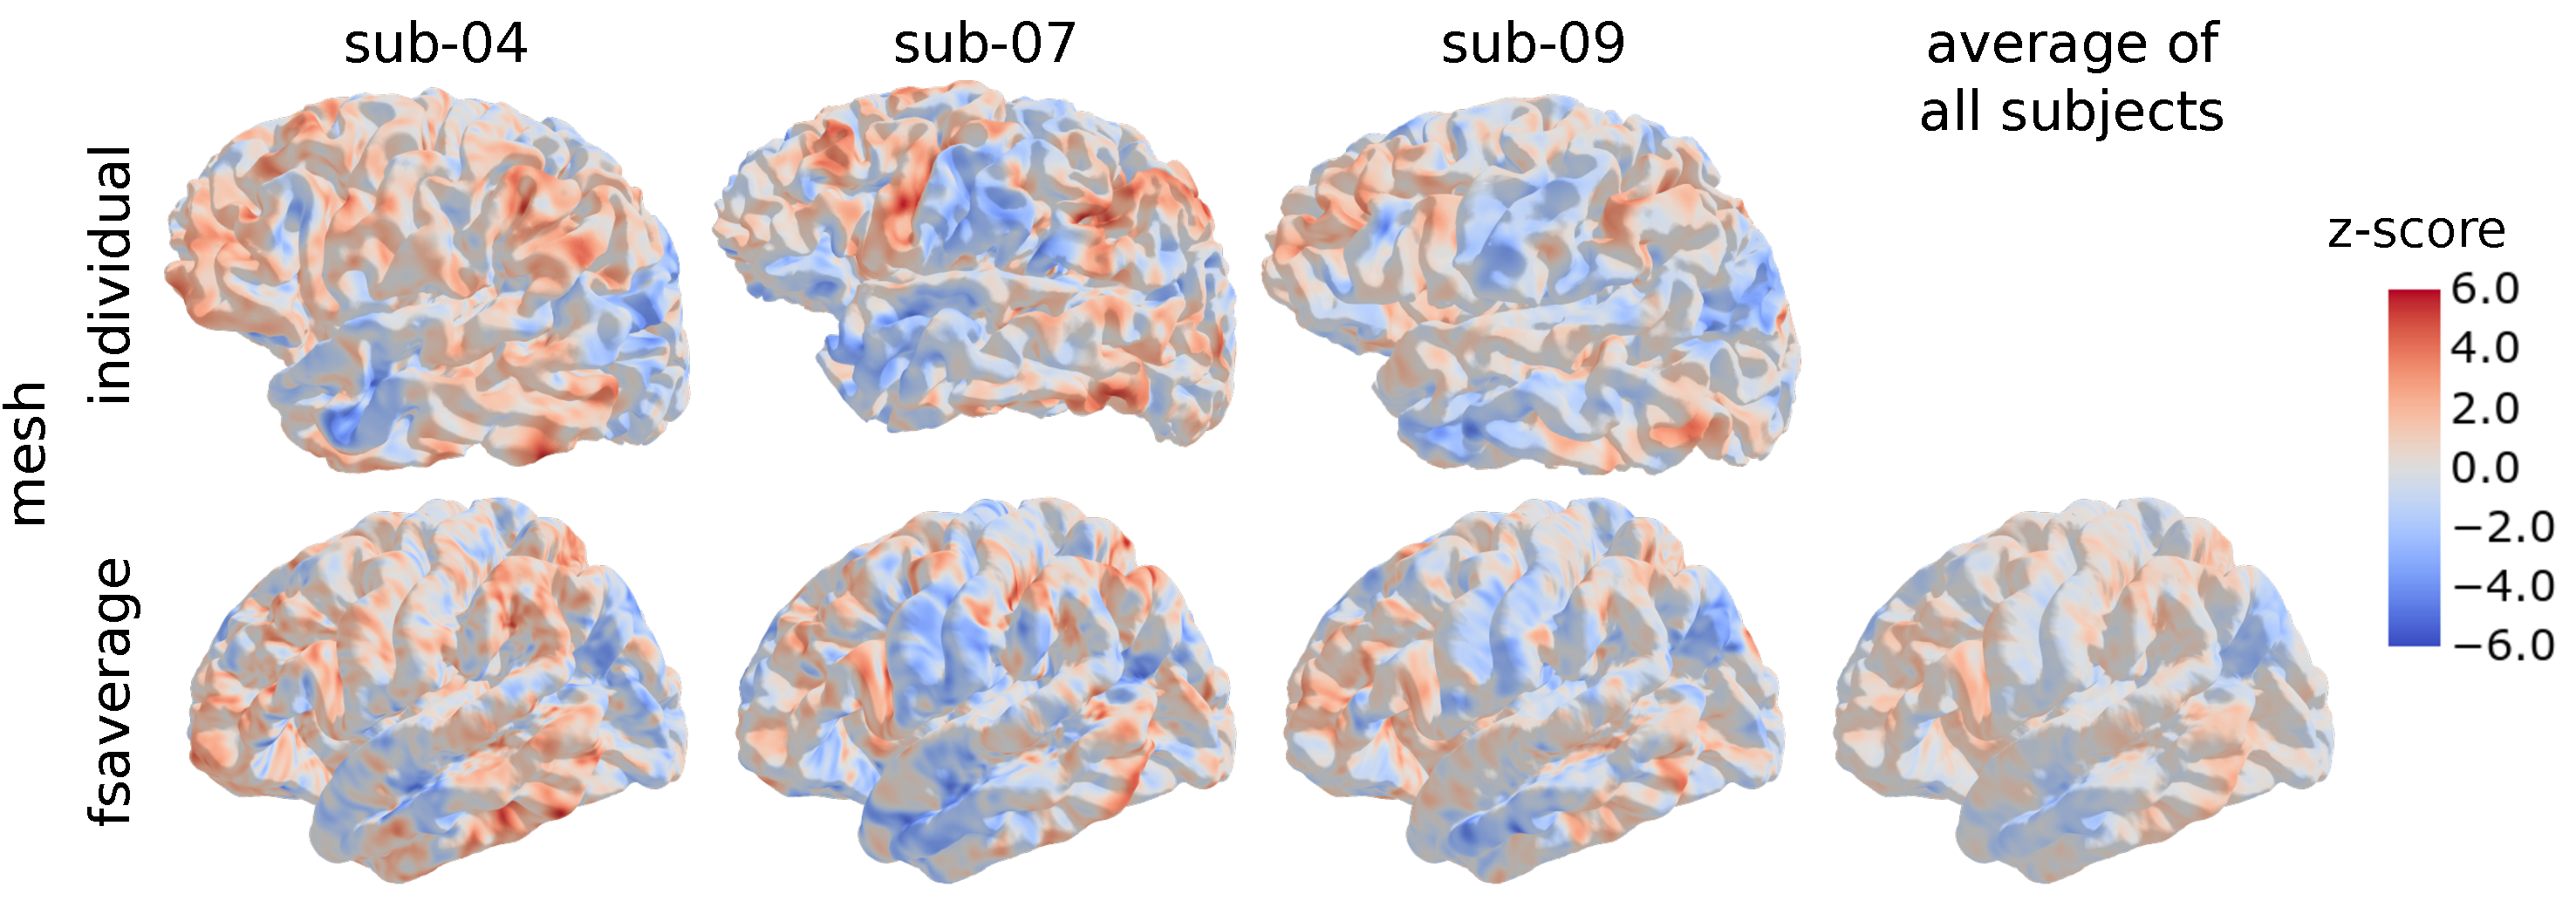
\includegraphics[width=\columnwidth]{./Chapitre4/figures/intro_variation.pdf}
    \caption[High variability in human anatomies and functional MRI responses across subjects]{
        \textbf{High variability in human anatomies and functional MRI responses across subjects}
        In this experiment contrasting areas of the brain
        which respond to mathematical tasks against other that
        don't, we observe great variability in locations and strength of brain activations across subjects (row 1).
        The classical approach consists in wrapping this data
        to a common surface template (row 2), where they can be averaged, often resulting in
        loss of individual details and detection power.
        These images were generated using Nilearn software \citep{abraham_machine_2014}.
    }
    \label{fig:intro}
\end{figure}
In order to improve upon the current situation, a number of challenges have to be addressed:
%
\textit{(i)} There exists no template brain with functional information,
which by construction renders any cortical matching method blind to function.
This is unfortunate, since functional information is arguably the most accessible marker
to identify cortical regions and their boundaries \citep{Glasser2016-ha}.
%
\textit{(ii)} When comparing two brains -- coming from individuals or from a template --
it is unclear what regularity should be imposed on the matching \citep{vanessen2012}.
While it is traditional in medical imaging to impose diffeomorphicity \citep{ants},
such a constrain does not match the frequent observation that brain regions vary
across individuals in their fine-grained functional organization \citep{Glasser2016-ha,schneider2019}.
% \bt{find other ref}
%
\textit{(iii)} Beyond the problem of aligning human brains, it is an even greater challenge
to systematically compare functional brain organization in two different species,
such as humans and macaques \citep{neubert_comparison_2014,mars_whole_2018,xu_cross-species_2020,eichert_cross-species_2020,}.
Such inter-species comparisons introduce a more extreme form of variability in the correspondence model.

\paragraph{Related work}
%
Several attempts have been made to constrain the brain alignment process by using
functional information. The first one consists in introducing functional maps into
the diffeomorphic framework and search for a smooth transformation that matches
functional information \citep{sabuncu_function-based_2010,yeo_spherical_2010,robinson_msm_2014},
the most popular framework being arguably Multimodal Surface Matching (MSM)
\citep{robinson_msm_2014,Glasser2016-ha}.

A second family of less constrained functional alignment approaches have been proposed,
based on heuristics, by matching information in small, possibly overlapping,
cortical patches \citep{haxby_common_2011,Tavor2016-rl,bazeille_empirical_2021}.
%
This popular framework has been called \emph{hyperalignment}
\citep{haxby_common_2011,guntupalli_model_2016}, or \emph{shared response models} \citep{Chen2015}.
%
Yet these approaches lack a principled framework and cannot be considered to solve
the matching problem at scale. Neither do they allow to estimate %
a group-level template properly \citep{alwasity2020}.

An alternative functional alignment framework has followed another path \citep{gramfort2015},
considering functional signal as a three-dimensional distribution, and minimizing the transport cost.
However, this framework imposes unnatural constraints of non-negativity of the signal and % approximate normalization.
only works for one-dimensional contrasts, so that it cannot be used to learn
multi-dimensional anatomo-functional structures.
%
An important limitation of the latter two families of methods is that they operate on
a fixed spatial context (mesh or voxel grid), and thus cannot be used on heterogeneous meshes
such as between two individual human anatomies or, worse, between a monkey brain
and a human brain.

\paragraph{Contributions}

Following \citep{bazeille_local_2019}, we use the Wasserstein distance between source and
target functional signals -- consisting of contrast maps acquired with fMRI --
to compute brain alignments. We contribute two notable extensions of this framework:
\textit{(i)} a Gromov-Wasserstein (GW) term to preserve global anatomical structure --
this term introduces an anatomical penalization against improbably distant anatomical matches,
yet without imposing diffeomorphic regularity -- as well as
\textit{(ii)} an unbalanced correspondence that allows mappings from one brain to another
to be incomplete, for instance because some functional areas are larger in some individuals
than in others, or may simply be absent. We show that this approach successfully addresses
the challenging case of different cortical meshes, and that derived brain activity templates
are sharper than those obtained with standard anatomical alignment approaches.

\section{Methods}
\label{sec:methods}

Optimal Transport yields a natural framework to address the alignment problem,
as it seeks to derive a plan -- a \textit{coupling} -- that can be seen as a soft assignment matrix
between cortical areas of a source and target individual.
As discussed previously, there is a need for a functional alignment method that respects
the rich geometric structure of the anatomical features, hence the Wasserstein distance alone
is not sufficient. By construction, the GW distance \citep{Memoli11,Memoli07}
can help preserve the global geometry underlying the signal.
The more recent fused GW distance \citep{Vayer19b} goes one step further by
making it possible to integrate functional data simultaneously with anatomical information.

\subsection{Fused Unbalanced Gromov-Wasserstein}

We leverage \citep{Vayer19b,Sejourne20} to present a new objective function which interpolates
between a loss preserving the global geometry of the underlying mesh structure and
a loss aligning source and target features, while simultaneously allowing not to transport
some parts of the source and target distributions. We provide an open-source solver
that minimizes this loss
\footnote{\href{https://github.com/alexisthual/fugw}{https://github.com/alexisthual/fugw}
provides a PyTorch \citep{NEURIPS2019_9015} solver with a scikit-learn \citep{scikit-learn}
compatible API}.

\paragraph{Formulation}
We denote $F^s \in \bbR^{n \times c}$ the matrix of features per vertex for the source subject.
In the proposed application, they correspond to $c$ functional activation maps,
sampled on a mesh with $n$ vertices representing the source subject's cortical surface.
Let $D^s \in \bbR^{n \times n}_+$ be the matrix of pairwise geodesic distances
\footnote{We compute geodesic distances using
\href{https://github.com/the-virtual-brain/tvb-gdist}{https://github.com/the-virtual-brain/tvb-gdist}}
between vertices of the source mesh.
Moreover, we assign the distribution $w^s \in \bbR^{n}_+$ on the source vertices.
Comparably, we define $F^t \in \bbR^{p \times c}$, $D^t \in \bbR^{p \times p}_+$ and
$w^t \in \bbR^{p}_+$ for the target subject, whose individual anatomy is represented
by a mesh comprising $p$ vertices.
Eventually, $w^s$ and $w^t$ set the transportable mass per vertex, which,
without prior knowledge, we choose to be uniform for the source and target vertices respectively:
$w^s \triangleq (\frac{1}{n}, ..., \frac{1}{n})$,
$w^t \triangleq (\frac{1}{p}, ..., \frac{1}{p})$.

Given a tuple of hyper-parameters $\theta \triangleq (\rho, \alpha, \varepsilon)$,
where $\rho, \varepsilon \in \bbR_+$ and $\alpha \in [0,1]$,
for any coupling $P \in \bbR^{n \times p}_{\geq 0}$,
we define the fused unbalanced Gromov-Wasserstein loss as
\begin{equation}
    \label{eq:fugw_obj_func}
    \begin{split}
        L_{\theta}(P) &=
        (1 - \alpha) \underbrace{\sum_{i,j} || F^s_i - F^t_j||_2^2 P_{ij}}_{\text{Wasserstein loss } L_{\text{W}}(P)}
        + \alpha \underbrace{\sum_{i,j,k,l} | D^s_{ik} - D^t_{jl}|^2 P_{ij} P_{kl}}_{\text{Gromov-Wasserstein loss } L_{\gw}(P)} \\
        &+ \rho \underbrace{\left[ \kl(P_{\# 1} \otimes P_{\# 1} \vert w^s \otimes w^s)
        + \kl(P_{\# 2} \otimes P_{\# 2} \vert w^t \otimes w^t) \right]}_{\text{Marginal constraints } L_{\text{U}}(P)}
        + \varepsilon \underbrace{E(P)}_{\text{Entropy}}
    \end{split}
\end{equation}
where $L_{\text{W}}(P)$ matches vertices with similar features,
$L_{\gw}(P)$ penalizes changes in geometry
and $L_{\text{U}}(P)$ fosters matching all parts of the source and target distributions.
Throughout this paper, we refer to relaxing the hard marginal constraints of the underlying
OT problem into soft ones as \textit{unbalancing}.
Here, $P_{\# 1} \triangleq (\sum_j P_{i,j})_{0 \leq i < n}$ denotes
the first marginal distribution of $P$,
and $P_{\# 2} \triangleq (\sum_i P_{i,j})_{0 \leq j < p}$
the second marginal distribution of $P$. The notation $\otimes$ represents
the Kronecker product between two vectors or two matrices.
$\kl(\cdot|\cdot)$ denotes the Kullback Leibler divergence,
which is a typical choice to measure the discrepancy between two measures
in the context of unbalanced optimal transport \citep{Liero18}.
The last term $E(P) \triangleq \kl \big(P \otimes P | (w^s \otimes w^t) \otimes (w^s \otimes w^t)\big)$
is mainly introduced for computational purposes, as it helps accelerate
the approximation scheme of the optimisation problem. Typically,
it is used in combination with a small value of $\varepsilon$,
so that the impact of other terms is not diluted. On the other hand,
the parameters $\alpha$ and $\rho$ offer control over two other aspects of the problem:
while $\alpha$ realizes a trade-off between the impact of different features and
different geometries in the resulting alignment, $\rho$ controls the amount of
mass transported by penalizing configurations such that the marginal distributions
of the transportation plan $P$ are far from the prior weights $w^s$ and $w^t$.
This potentially helps adapting the size of areas where either the signal or the geometry
differs too much between source and target.

Eventually, we define $\cX^s \triangleq (F^s, D^s, w^s)$ and $\cX^t \triangleq (F^t, D^t, w^t)$,
and seek to derive an optimal coupling $P \in \bbR^{n \times p}_{\geq 0}$ minimizing
\begin{equation}
    \label{eq:fugw}
    \begin{split}
        \fugw(\cX^s, \cX^t)
        &\triangleq \inf_{P \in \bbR^{n \times p}_{\geq 0}} L_{\theta}(P).
    \end{split}
\end{equation}
This can be seen as a natural combination of the fused GW \citep{Vayer19b}
and the unbalanced GW \citep{Sejourne20} distances. To the best of our knowledge,
it has never been considered in the literature.

\paragraph{Toy example illustrating the unbalancing property}

As exemplified in \Cref{fig:intro}, brain responses elicited by the same stimulus
vary greatly between individuals.
\Cref{fig:toy_example} illustrates a similar yet simplified version of this problem,
where the goal is to align two different signals  supported on the same spherical meshes.
In this example, for each of the $n=p=3200$ vertices, the feature is simply a scalar.
On the source mesh, the signal is constituted of two von Mises density functions that differ
by their concentration (large and small), while on the target mesh, only the large one is present,
but at a different location.
We use the optimal coupling matrix $P$ obtained from Equation \eqref{eq:fugw} to transport
the source signal on the target mesh.
As shown in \Cref{fig:toy_example}.B, the parameter $\rho$ allows to control
the mass transferred from source to target.
When $\rho=100$, we approach the solution of the fused GW problem. Consequently,
we observe the second mode on the target when transporting the source signal.
When the mass control is weaker ($\rho=1$), the smaller blob is partly removed because
it has no counterpart in the target configuration, making the transport ill-posed.
\iffalse This corresponds to a mass destruction, as depicted on the right of the Figure,
whereas the larger blob in the target distribution is also a place of mass creation. \fi

\begin{figure}[t]
    \centering
    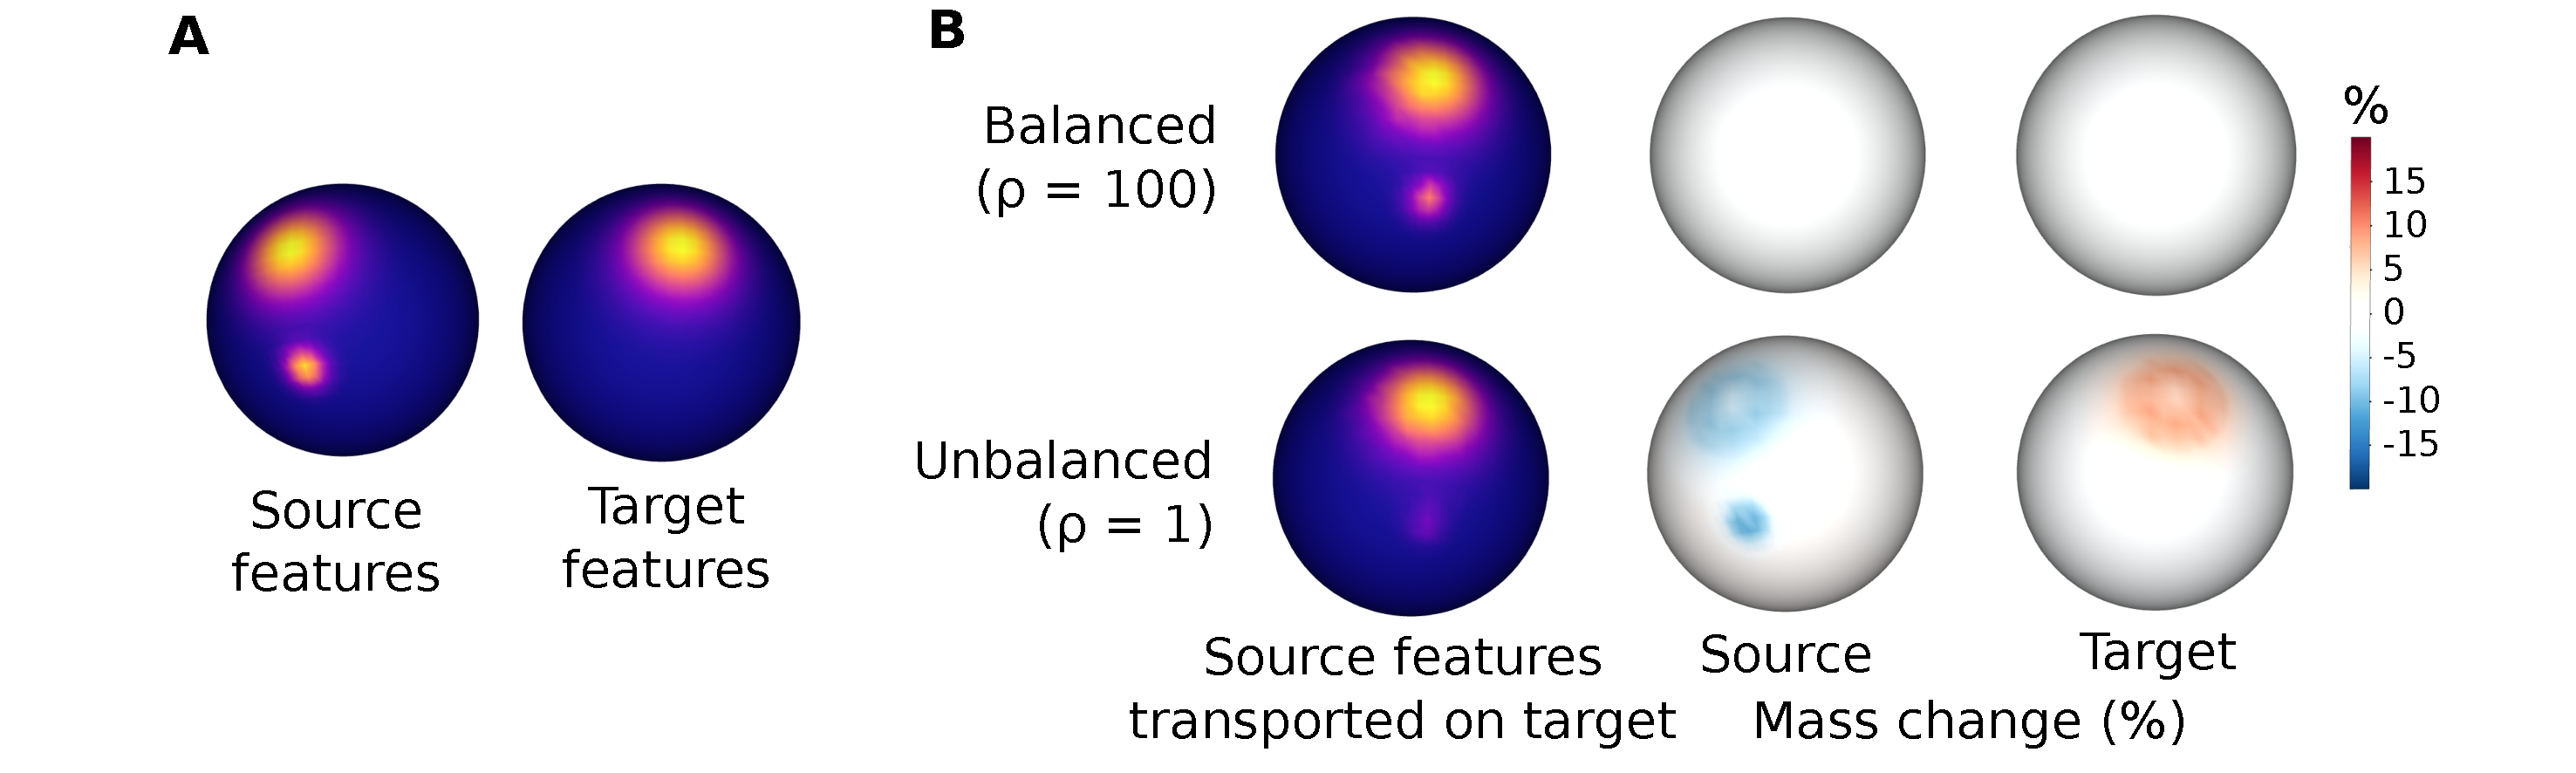
\includegraphics[width=1\columnwidth]{./Chapitre4/figures/toy_example.pdf}
    \caption[Unbalancing helps accounting for idiosyncrasies of the source and target signals]{
        \textbf{Unbalancing helps accounting for idiosyncrasies of the source and target signals}
        When trying to align the source and target signals (Panel A),
        the classical balanced setup (Panel B, top row) transports all parts of
        the source signal even if they have no counterpart in the target signal.
        In the unbalanced setup (Panel B, bottom row), less source-only signal is transported:
        in particular, less mass is transported from the source's small blob onto the target
        (Panel B, middle column).
    }
    \label{fig:toy_example}
\end{figure}

%%%%%%%%%%%%%%%%%%%%%%%%%%%%%%%%%%%%%%%%%%
\subsection{Optimization}

Estimating the unbalanced Gromov Wasserstein loss is numerically sensitive to initialization,
due to the non-convexity of the problem.
Therefore, FUGW is also \textit{a priori} non-convex, and comparably difficult to estimate.
Consequently, following \citep{Sejourne20}, we instead compute a lower bound which
is formulated as a bi-convex problem that relies on the joint estimation of two couplings.
\begin{align}
    \label{eq:lbfugw}
    \quad \fugw(\cX^s, \cX^t) = \inf_{\substack{P, Q \in \bbR^{n \times p}_{\geq 0} \\ P = Q}}
    L_{\theta}(P, Q) \geq \inf_{\substack{P, Q \in \bbR^{n \times p}_{\geq 0} \\ m(P) = m(Q)}}
    L_{\theta}(P, Q) \triangleq \text{LB-FUGW} (\cX^s, \cX^t),
\end{align}
where $m(P) = \sum_{i,j} P_{i,j}$ denotes the mass of $P$ and
\begin{equation}
    \label{eq:fugw_loss_two_couplings}
    \begin{split}
        L_{\theta}(P, Q) \triangleq
        (1 - \alpha) \enspace L_{\text{W}}(P, Q) + \alpha \enspace L_{\gw}(P, Q)
        + \rho \enspace L_{\text{U}}(P, Q) + \varepsilon \enspace E(P, Q),
    \end{split}
\end{equation}
where
\begin{itemize}
    \item[$\bullet$] $C \triangleq \Big( ||F^s_{i} - F^t_j||^2_2\Big)_{i,j} \in \bbR^2_+$ \hfill (feature cost matrix)

    \item[$\bullet$] $G \triangleq \Big( |D^s_{i,j} - D^t_{k,l}| \Big)_{i,j,k,l} \in \bbR^4_+$ \hfill (geometry cost tensor)

    \item[$\bullet$] $L_{\text{W}}(P, Q) \triangleq \langle C, \frac{P + Q}{2} \rangle = \frac{1}{2} ( \sum_{i,j} C_{i,j}P_{i,j} + \sum_{i,j} C_{i,j}Q_{i,j})$ \hfill (Wasserstein)

    \item[$\bullet$] $L_{\gw}(P, Q) \triangleq \langle G , P \otimes Q \rangle = \sum_{i,j,k,l}G_{i,j,k,l}P_{i,j}Q_{k,l}$ \hfill (Gromov-Wasserstein)

    \item[$\bullet$] $L_{\text{U}}(P, Q) \triangleq \enspace \kl \Big(P_{\# 1} \otimes Q_{\# 1} \vert w^s \otimes w^s \Big) + \enspace \kl \Big(P_{\# 2} \otimes Q_{\# 2} \vert w^t \otimes w^t \Big)$ \hfill (unbalancing)

    \item[$\bullet$] $E(P, Q) \triangleq \kl \Big(P \otimes Q | (w^s \otimes w^t) \otimes (w^s \otimes w^t) \Big)$ \hfill (entropy)
\end{itemize}
In particular, we have $L_{\theta}(P, P) = L_{\theta}(P)$,
which is the objective function of FUGW introduced in Equation \eqref{eq:fugw_obj_func}.
It is difficult to study when equality holds between FUGW and its lower bound.
Here, we attempt to understand the potential gap between them.
First, let us introduce the following problem
\begin{equation}
  \widetilde{\fugw}(\cX^s, \cX^t) = \inf_{(P, Q) \in \cE} L_{\theta}(P, Q),
\end{equation}
where $\cE = \{P, Q \in \bbR^{n \times p}_{\geq 0}: P_{\#1} = Q_{\#1}, P_{\#2} = Q_{\#2} \}$ is
the set of pairs of transportation plans whose corresponding marginal distributions are equal.
Clearly, we have
\begin{equation}
    \text{LB-FUGW} (\cX^s, \cX^t) \leq \widetilde{\fugw}(\cX^s, \cX^t)
    \leq \fugw(\cX^s, \cX^t).
\end{equation}
This inequality indicates that the difference between FUGW and LB-FUGW might be potentially large.
However, this gap can be tightened under the conditions in \Cref{prop:coot_gw_equiv}.
%%%%%%%%%%%%%%%%%%%%%%%%%%%%%%%%%%%%%%%%%%%%%
\begin{corollary} \label{coro:ugw_ucoot}
    If the distances $D^s$ and $D^t$ are of the forms: $D^s_{ij} = f_i + f_j + A_{ij}$ and
    $D^t_{kl} = g_k + g_l + B_{kl}$, where $f, g$ are vectors in $\bbR^n, \bbR^p$, respectively,
    and the matrices $A, B$ are both conditionally negative semi-definite, then we have
    $\fugw (\cX^s, \cX^t) = \widetilde{\fugw}(\cX^s, \cX^t)$.
    % Furthermore, if the definiteness holds, then the optimal solution satisfies $P^* = Q^*$,
    % meaning that $\text{LB-FUGW} (\cX^s, \cX^t) = \fugw(\cX^s, \cX^t)$.
\end{corollary}
%%%%%%%%%%%%%%%%%%%%%%%%%%%%%%%%%%%%%%%%%%%%%%%%
% In our experiments, while the geodesic distances do not necessarily meet these conditions,
In our experiments, while the geodesic distances do not necessarily meet these conditions,
we still observe that the two couplings of LB-FUGW are numerically equal.
So it is enough to choose, for example, the first one, as alignment between source and target signals.

The lower bound of FUGW \eqref{eq:lbfugw} involves solving a minimization problem with respect to two independent couplings.
Using a Block-Coordinate Descent (BCD) scheme, we fix a coupling and minimize
with respect to the other. This allows us to always be dealing with linear problems
instead of a quadratic one. Eventually, each BCD iteration consists in alternatively solving
two entropic unbalanced OT problems, whose solutions can be approximated using
the Sinkhorn algorithm \citep{Sejourne19}.

%%%%%%%%%%%%%%%%%%%%%%%%%%%%%%
\subsection{FUGW Barycenters}
Barycenters represent common patterns across samples.
Their role is instrumental in identifying a unique target for aligning a given group of individuals.
As seen in \Cref{fig:intro}, the vertex-wise group average does not usually provide
well-contrasted maps.
Inspired by the success of the GW distance when estimating the barycenter of structured objects
\citep{Peyre16,Vayer19b}, we use FUGW to find the barycenter
$(F^B, D^B) \in \bbR^{k \times c} \times \bbR^{k \times k}$
of all subjects $s \in \cS$, as well as the corresponding couplings $P^{s,B}$ from each subject
to the barycenter. More precisely, we solve
\begin{equation}
    \label{eq:barycenter}
    \cX^B = (F^B, D^B, w^B) \in \argmin_{\cX}  \sum_{s \in \cS} \fugw(\cX^s, \cX),
\end{equation}
where we set the weights $w_B$ to be the uniform distribution.
By construction, the resulting barycenter benefits from the advantages of FUGW,
i.e. equilibrium between geometry-preserving and feature-matching properties,
while not forcing hard marginal constraints. The FUGW barycenter is estimated
using a Block-Coordinate Descent (BCD) algorithm that consists in alternatively
\textit{(i)} minimizing the OT plans $P^{s,B}$ for each FUGW computation
in \eqref{eq:barycenter} with fixed $\cX^B$ and \textit{(ii)}
updating the barycenter $\cX^B$ through a closed form with fixed $P^{s,B}$.
See \Cref{alg:fugw_barycenter} for more details.
The first step simply uses the previously introduced solver.
The second one takes advantage of the fact that the objective function introduced
in \eqref{eq:lbfugw} is differentiable in $F^B$ and $D^B$, and the two couplings of
LB-FUGW are numerically equal. This yields a closed form for $F^B$ and $D^B$,
as a function of $P^{s,B}$ and $\cX^s$. We note that, during the barycenter estimation,
the weight $w^B$ is always fixed as uniform distribution.

\begin{algorithm}[t]
    \caption{LB-FUGW barycenter for Problem \eqref{eq:barycenter}}
    \label{alg:fugw_barycenter}
    \begin{algorithmic}[1]
        \STATE \textbf{Input:} $(\cX^s)_{s \in \cS}, \rho, \alpha, \varepsilon$.
        \STATE \textbf{Output:} Individual couplings $(P^{s, B})_{s \in \cS}$, barycenter $\cX^B$.
        \STATE Initialize: $F^B = \mathbb I_k$; $D^B = 0_k$.
        \WHILE{$\cX^B = (F^B, D^B, w^B)$ has not converged}
            \STATE Draw $\widetilde{S}$ subset of $S$.
            \FOR{$s \in \widetilde{S}$}
                \STATE Align: $P^{s, B} \gets \text{LB-FUGW}(\cX^s, \cX^B, \rho, \alpha, \varepsilon)$.
                \COMMENT{Fixed $\cX^B$}
            \ENDFOR
            \STATE Update $F^B$, $D^B$:
            \COMMENT{Fixed $P^{s, B}$}
            \begin{equation*}
                F^B = \frac{1}{| \widetilde{S} |} \sum_{s \in \widetilde{S}}
                \text{diag} \left( \frac{1}{P^{s, B}_{\# 2}} \right)
                (P^{s, B})^\top F^s \; \text{ and } \;
                D_B = \frac{1}{| \widetilde{S} |} \sum_{s \in \widetilde{S}}
                \frac{(P^{s, B})^\top D^s P^{s, B}}{P^{s, B}_{\# 2} (P^{s, B}_{\# 2})^\top}.
            \end{equation*}
        \ENDWHILE
    \end{algorithmic}
\end{algorithm}

%%%%%%%%%%%%%%%%%%%%%%%%%%%%%%%%%%%%%%%%%ù
\section{Numerical experiments}

We design three experiments to assess the performance of FUGW.
In Experiments 1 and 2, we are interested in assessing if aligning pairs of individuals with
FUGW increases correlation between subjects compared to a baseline correlation.
We also compare the ensuing gains with those obtained when using the
competing method MSM \citep{robinson_msm_2014,robinson_multimodal_2018} to align subjects.
In Experiment 3, we derive a barycenter of individuals and assess its ability to capture fine-grained
details compared to classical methods.

\subsection{Experimental settings}

\paragraph{Dataset}
\label{par:dataset}
In all three experiments, we leverage data from the Individual Brain Charting dataset \citep{ibc}.
It is a longitudinal study on 12 human subjects,
comprising 400 fMRI maps per subject collected
on a wide variety of stimuli (motor, visual, auditory, theory of mind,
language, mathematics, emotions, and more), movie-watching data, T1-weighted maps, as well as other features such as
retinotopy which we don't use in this work. We leverage these 400 fMRI maps.
The training, validation and test sets respectively comprise
326, 43 and 30 contrast maps acquired for each individual of the dataset.
Tasks and MRI sessions differ between each of the sets.
% More details, including preprocessing, are provided in Supplementary Materials.

\paragraph{Baseline alignment correlation}
For each pair of individuals $(s, t)$ under study, and for each fMRI contrast $c$ in the test set,
we compute the Pearson correlation $\text{corr}(F^s_{\cdot, c}, F^t_{\cdot, c})$
after these maps have been projected onto a common surface anatomy (in this case, \emph{fsaverage5}
mesh). Throughout this work, such computations are made for each hemisphere separately.

\paragraph{Experiment 1 - Aligning pairs of humans with the same anatomy}
%
For each pair $(s, t)$ under study, we derive an alignment $P^{s,t} \in \bbR^{n \times p}$
using FUGW on a set of training features. In this experiment, source and target data
lie on the same anatomical mesh (\emph{fsaverage5}), and $n = p = 10240$ for each hemisphere.
Since each hemisphere's mesh is connected, we align one hemisphere at a time.

Computed couplings are used to align contrast maps of a the validation set from
the source subject onto the target subject. Indeed, one can define
$\phi_{s \rightarrow t} \colon X \in \bbR^{n \times q}
\mapsto \big((P^{s,t})^T X \big) \oslash P^{s,t}_{\#2} \in \bbR^{p \times q}$
where $\oslash$ represents the element-wise division. $\phi_{s \rightarrow t}$
transports any matrix of features from the source mesh to the target mesh.
We measure the Pearson correlation $\text{corr}\big( \phi_{s \rightarrow t}(F^s), F^t \big)$
between each aligned source and target maps.

We run a similar experiment for MSM and compute the correlation gain induced on a
test set by FUGW and MSM respectively.
For both models, we selected the hyper-parameters maximizing correlation gain on a validation set.
In the case of FUGW, in addition to gains in correlation, hyper-parameter selection
was influenced by three other metrics that help us assess the relevance of computed couplings:

\begin{description}
    \item[Transported mass]
    For each vertex $i$ of the source subject, we compute
    $\sum \limits_{0 \leq j < p} P^{s,t}_{i, j}$.

    \item[Vertex displacement]
    Taking advantage of the fact that the source and target anatomies are the same,
    we define $D = D^s = D^t$ and compute for each vertex $i$ of the source subject the quantity
    $\sum_j P^{s,t}_{i, j} \cdot D_{i, j} / \sum_j P^{s,t}_{i,j}$,
    which measures the average geodesic distance on the cortical sheet between vertex $i$
    and the vertices of the target it has been matched with.

    \item[Vertex spread]
    Large values of $\varepsilon$ increase the entropy of derived couplings.
    To quantify this effect, and because we don't want the matching to be too blurry,
    we assess how much a vertex was \textit{spread}. Considering
    $\tilde{P_i} = P^{s,t}_i / \sum_j P^{s,t}_{i,j} \in \bbR^p$
    as a probability measure on target vertices,
    we estimate the anatomical variance of this measure by sampling $q$ pairs
    $(j_q, k_q)$ of $\tilde{P_i}$ and computing their average geodesic distance
    $\frac{1}{q} \sum\limits_{j_q, k_q} D_{j_q, k_q}$.
\end{description}

\paragraph{Experiment 2 - Aligning pairs of humans with individual anatomies}
We perform a second alignment experiment, this time using individual meshes instead of
an anatomical template. Importantly, in this case,  there is no possibility to compare
FUGW with baseline methods, since those cannot handle this case.
However, individual meshes are significantly larger than the
common anatomical template used in Experiment 1 ($n \approx m \approx$ 160k vs. 10k previously),
resulting in couplings too large to fit on GPUs -- for reference,
a coupling of size 10k $\times$ 10k already weights ~400Mo on disk.
We thus reduce the size of the source and target data by
clustering them into 10k small connected clusters using Ward's algorithm \citep{thirion:2014}.
% More details are given in supplementary section A.4.

\paragraph{Experiment 3 - Comparing FUGW barycenters with usual group analysis}
\label{par:barycenter}

Since it is very difficult to estimate the barycentric mesh, we force it to be equal to
the \emph{fsaverage5} template. Empirically, this we force the distance matrix $D^B$
to be equal to that of \emph{fsaverage5}, and only estimate the functional barycenter $F^B$.
We initialize it with the mean of $(F^s)_{s \in S}$
and derive $F^B$ and $(P^{s,B})_{s \in S}$ from Problem \eqref{eq:barycenter}.
Then, for a given stimulus $c$, we compute its projection onto the barycenter for each subject.
We use these projections to compute two maps of interest:
\textit{(i)} $M_{B,c}$ the mean of projected contrast maps across subjects
and \textit{(ii)} $T_{B,c}$ the t-statistic (for each vertex) of projected maps.
We compare these two maps with their unaligned counterparts $M_{0,c}$ and $T_{0,c}$ respectively.
\begin{figure}[ht]
    \begin{minipage}{.4\linewidth}
        \begin{equation*}
            M_{B,c} \triangleq \frac{1}{|S|} \sum_{s \in S} \phi_{s \rightarrow t}(F^s_{\cdot, c})
        \end{equation*}
    \end{minipage}
    \hfil
    \begin{minipage}{.5\linewidth}
        \begin{equation*}
            T_{B,c} \triangleq \text{t-statistic} \Big( \big(
                \phi_{s \rightarrow t}(F^s_{\cdot, c}) \big)_{s \in S} \Big)
        \end{equation*}
    \end{minipage}
\end{figure}
% \vspace*{-0.5\baselineskip}
\begin{figure}[ht]
    \begin{minipage}{.4\linewidth}
        \begin{equation*}
            M_{0,c} \triangleq \frac{1}{|S|} \sum_{s \in S} F^s_{\cdot, c}
        \end{equation*}
    \end{minipage}
    \hfil
    \begin{minipage}{.5\linewidth}
        \begin{equation*}
            T_{0,c} \triangleq \text{t-statistic} \Big( (F^s_{\cdot, c})_{s \in S} \Big)
        \end{equation*}
    \end{minipage}
\end{figure}
The first map helps us to qualitatively evaluate the precision of FUGW alignments and barycenter.
The second one is classically used to infer the existence of areas of the brain that
respond to specific stimuli. We assess whether FUGW helps find the same clusters of vertices.
Eventually, we quantify the number of vertices significantly activated or deactivated
with and without alignment respectively.

%%%%%%%%%%%%%%%%%%%%%%%%%%%%%%%%%%%%%%%%%%%%%%%%%
\subsection{Experiment 1 - Template anatomy}

\paragraph{Aligning subjects on a fixed mesh}

We set $\alpha = 0.5$, $\rho = 1$ and $\varepsilon = 10^{-3}$.
Pearson correlation between source and target contrast maps is systematically and
significantly increased when aligned using FUGW, as illustrated in
\Cref{fig:gain_comparisions_fsaverage5} where correlation grows by almost $40\%$
from $0.258$ to $0.356$.

\begin{figure}[ht!]
    \centering
    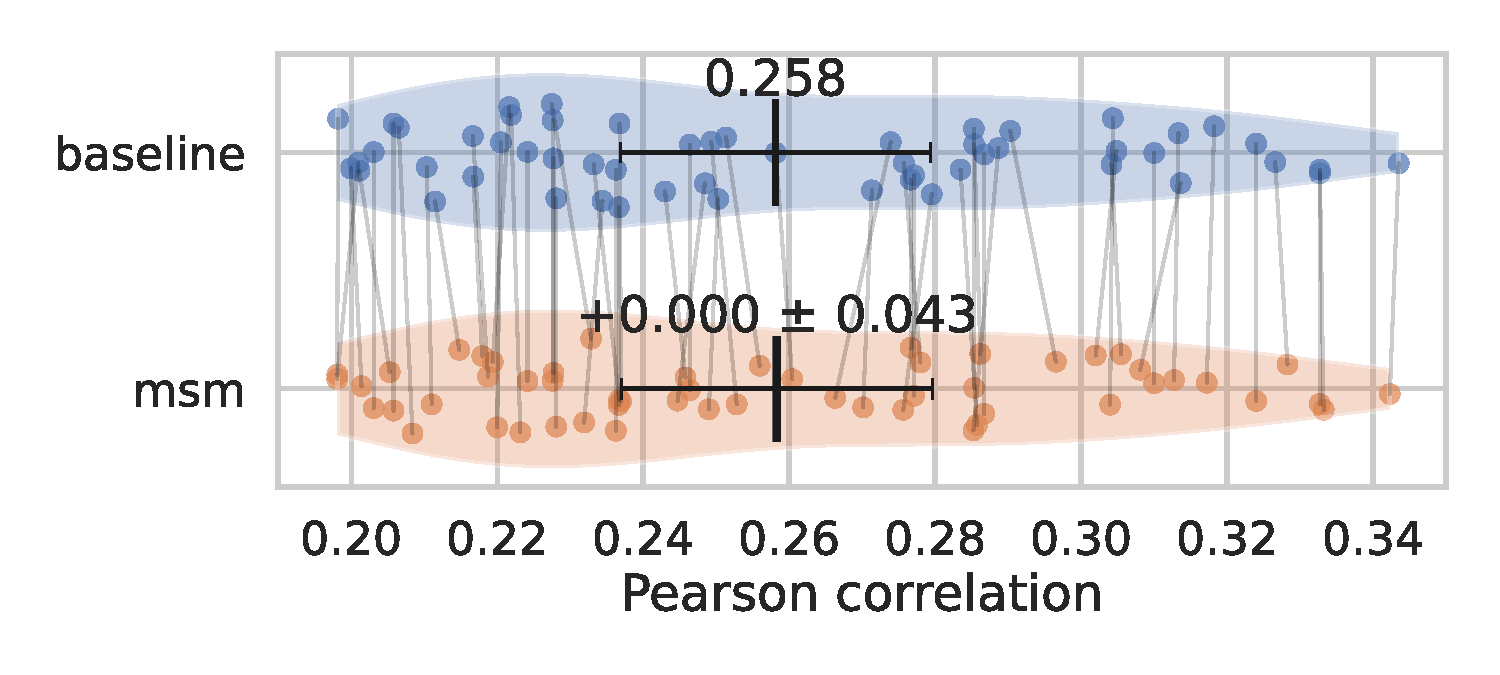
\includegraphics[width=0.49\columnwidth]{./Chapitre4/figures/fsaverage5_alignment_correlation_gain_msm.pdf}
    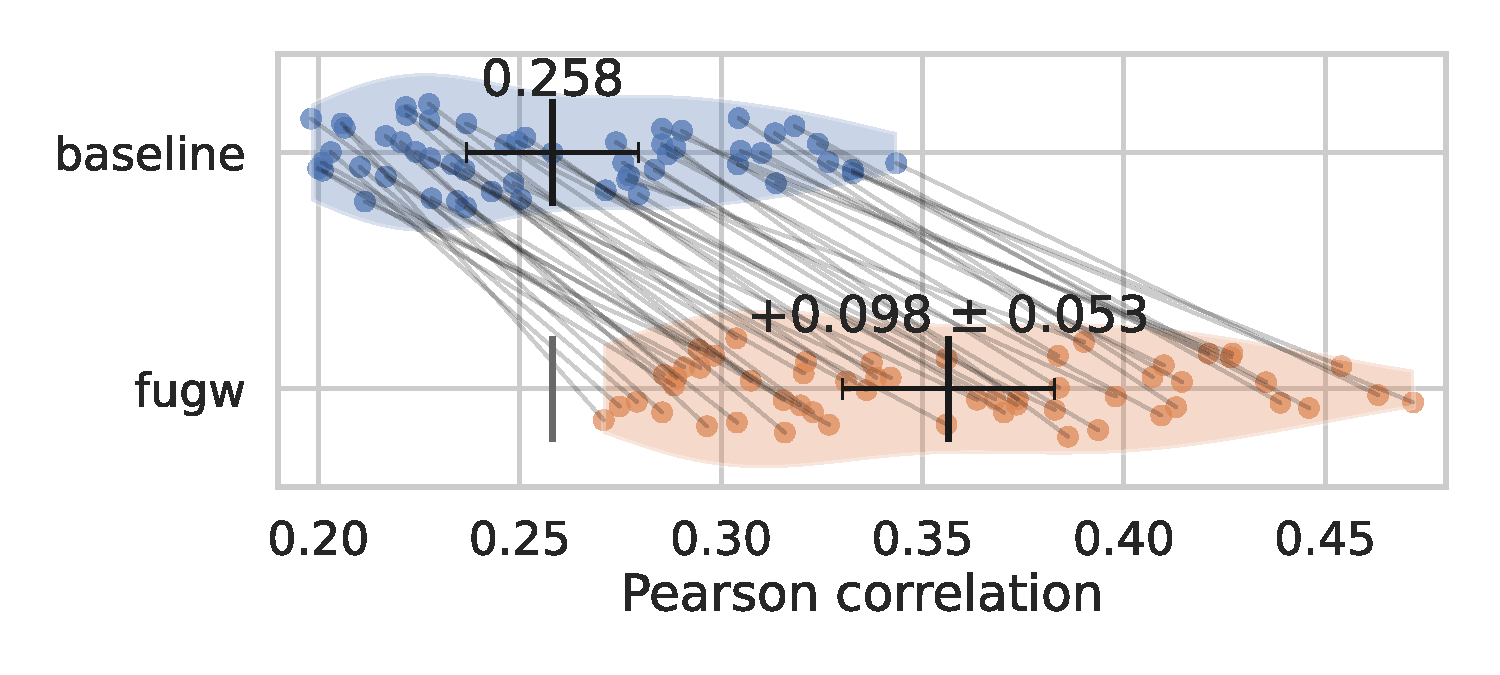
\includegraphics[width=0.49\columnwidth]{./Chapitre4/figures/fsaverage5_alignment_correlation_gain_fugw.pdf}
    \caption[Comparison of gains in correlation after inter-subject alignment]{
        \textbf{Comparison of gains in correlation after inter-subject alignment}
        For each pair of source and target subjects of the dataset,
        we compute the average Pearson correlation between 30 test contrasts,
        leading to the (baseline) correspondence score,
        and compare it with that of the same contrast maps
        aligned with either MSM (left) or FUGW (right). Correlation gains are much better for FUGW.
    }
    \label{fig:gain_comparisions_fsaverage5}
\end{figure}
% We also varied training sets by selecting subsets of training contrasts and find that
% similar performance on the test set can be achieved regardless of the training data
% (see Supplementary \Cref{sec:control_experiments} and in particular Supplementary
% \Cref{tab:varying_training_sets}).

\paragraph{Hyper-parameters selection}
\label{par:params_selection}

Hyper-parameters used to obtain these results were chosen
after running a grid search on $\alpha$, $\varepsilon$ and $\rho$
and evaluating it on the validation dataset.
Computation took about 100 hours using 4 Tesla V100-DGXS-32GB GPUs. More precisely,
it takes about 4 minutes to compute one coupling between a source and target 10k-vertex
hemisphere on a single GPU, when the solver was set to run 10 BCD and 400 Sinkhorn iterations.
In comparison, MSM takes about the same time on Intel(R) Xeon(R) CPU E5-2698 v4 @ 2.20GHz CPUs.
Results are reported in \Cref{fig:cv_metrics} and provide multiple insights concerning FUGW.

Firstly, without anatomical constraint ($\alpha = 0$),
source vertices can be matched with target vertices
that are arbitrarily far on the cortical sheet.
Even though this can significantly increase correlation, it also
results in very high vertex displacement values (up to $100mm$).
Such couplings are not anatomically plausible.
%
Secondly, without functional information ($\alpha = 1$),
couplings recover a nearly flawless matching between source and target meshes,
so that, when $\varepsilon = 10^{-5}$
(ie when we force couplings to find single-vertex-to-single-vertex matches),
vertex displacement and spread are close to 0 and correlation is unchanged.
%
Fusing both constraints ($0 < \alpha < 1$)
yields the largest gains in correlation while allowing to compute
anatomically plausible reorganizations the cortical sheet between subjects.

The impact of $\rho$ (controlling marginal penalizations) on correlation seems modest,
with a slight tendency of increased correlation in unbalanced problems (low $\rho$).

Finally, it is worth noting that a relatively wide range of $\alpha$ and $\rho$ yield comparable gains.
The fact that FUGW performance is weakly sensitive to hyper-parameters makes it
a good off-the-shelf tool for neuroscientists who wish to derive inter-individual alignments.
However, $\varepsilon$ is of dramatic importance in computed results and should be chosen carefully.
Vertex spread is a useful metric to choose sensible values of $\varepsilon$;
for human data one might consider that it should not exceed $20mm$.

\begin{figure}[ht]
    \centering
    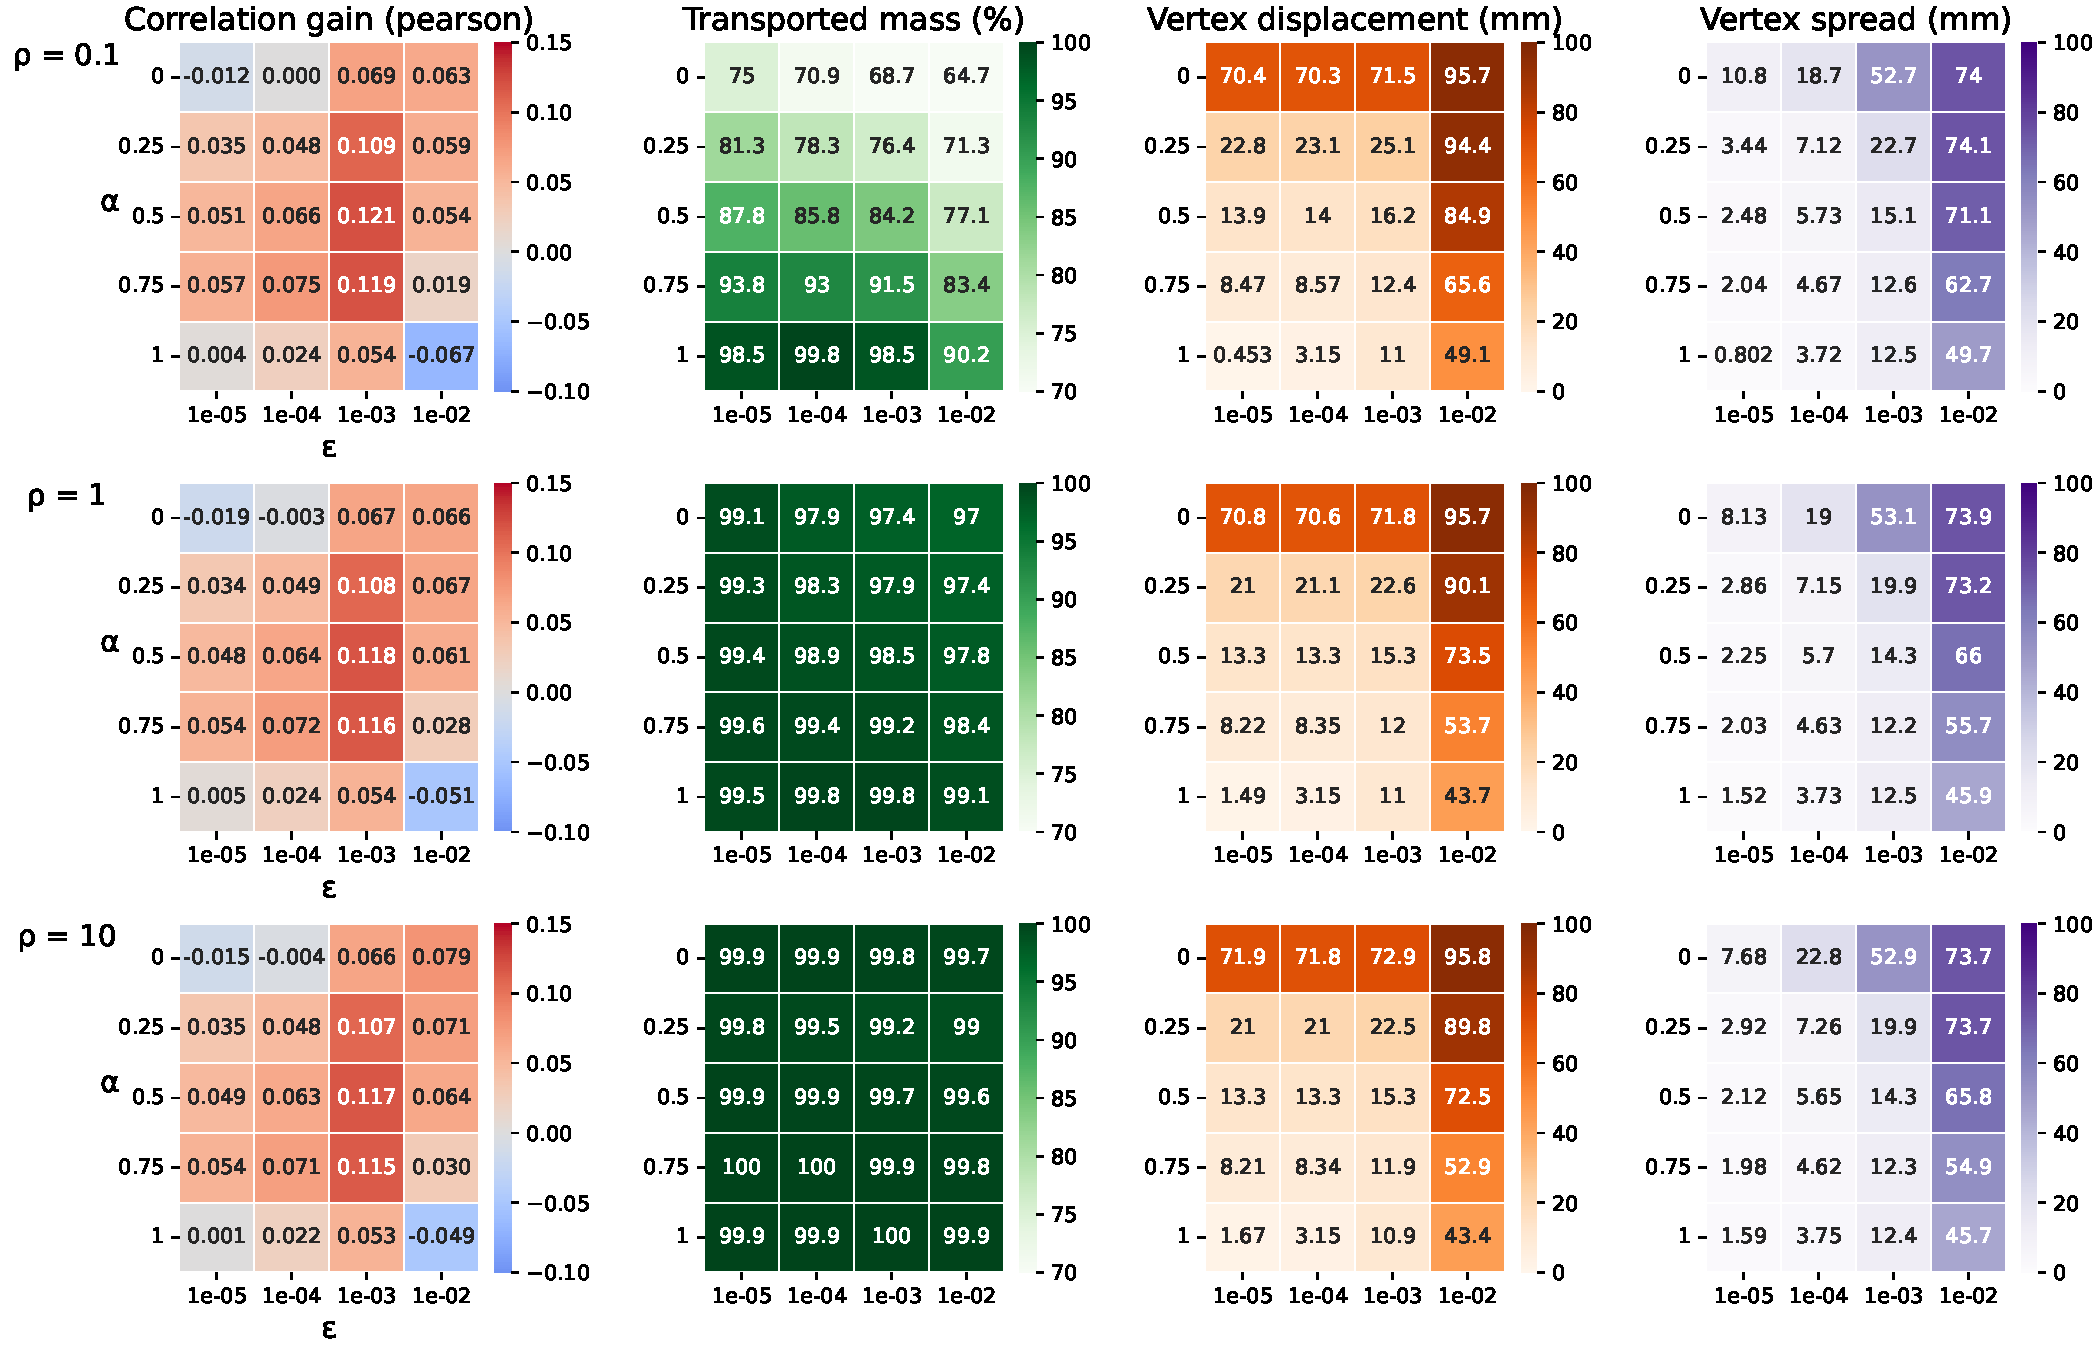
\includegraphics[width=1\columnwidth]{./Chapitre4/figures/cv_all_metrics_hcp_left_fugw.pdf}
    \caption[Exploring hyper-parameter space to find relevant couplings]{
        \textbf{Exploring hyper-parameter space to find relevant couplings}
        Given a transport plan aligning a source and target subject,
        we evaluate how much this coupling
        (left) improves correlation between unseen contrast maps
        of the two subjects,
        (center left) actually transports data,
        (center right) moves vertices far from their original location on the cortical surface
        and (right) spreads vertices on the cortical sheet.
        We seek plans that maximize correlation gain, while keeping spread and displacement low enough.
    }
    \label{fig:cv_metrics}
\end{figure}

\paragraph{Mass redistribution in unbalanced couplings}
Unbalanced couplings provide additional information about how functional areas might differ
in size between pairs of individuals. This is illustrated in \Cref{fig:transported_mass},
where we observe variation in size of the auditory area between a given pair of individuals.
This feature is indeed captured by the difference of mass between subjects
(although the displayed contrast was not part of the training set).
\begin{figure}[!th]
    \centering
    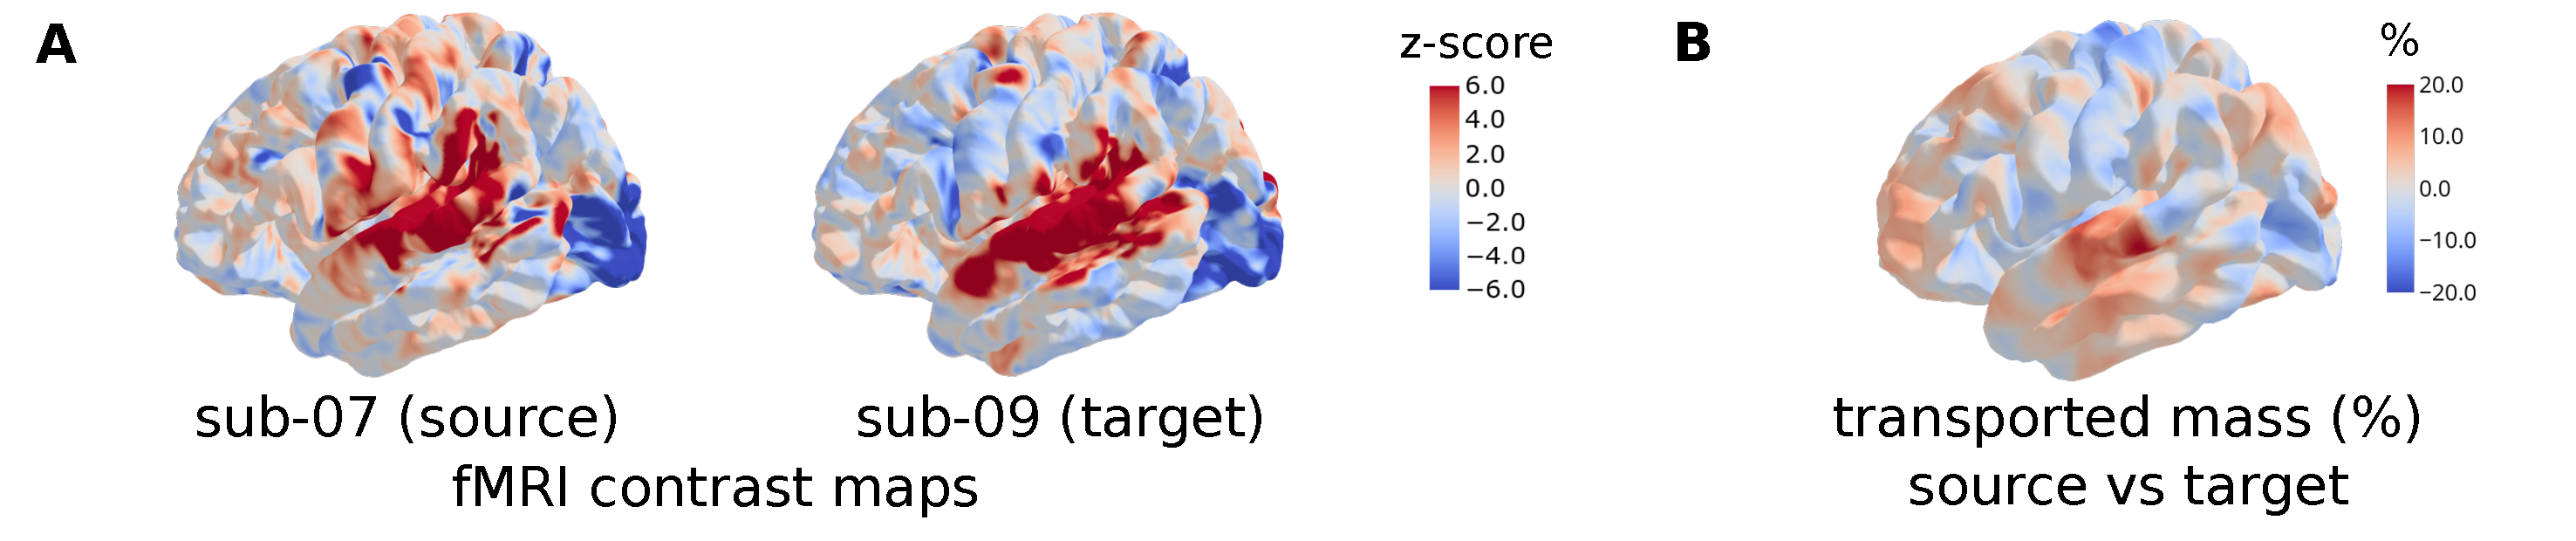
\includegraphics[width=1\columnwidth]{./Chapitre4/figures/transported_mass.pdf}
    \caption[Transported mass indicates areas which have to be resized between subjects]{
        \textbf{Transported mass indicates areas which have to be resized between subjects}
        (Panel A) We show a contrast map from the test set which displays areas showing
        stronger activation during auditory tasks versus equivalent visual tasks. It shows much more
        anterior activations on the target subject compared to the source subject.
        This is consistent with the observation that more mass is present in
        anterior auditory areas of the source subject than in the target subject (Panel B).
    }
    \label{fig:transported_mass}
\end{figure}

\subsection{Experiment 2 - Individual anatomies}
\begin{figure}[!ht]
    \centering
    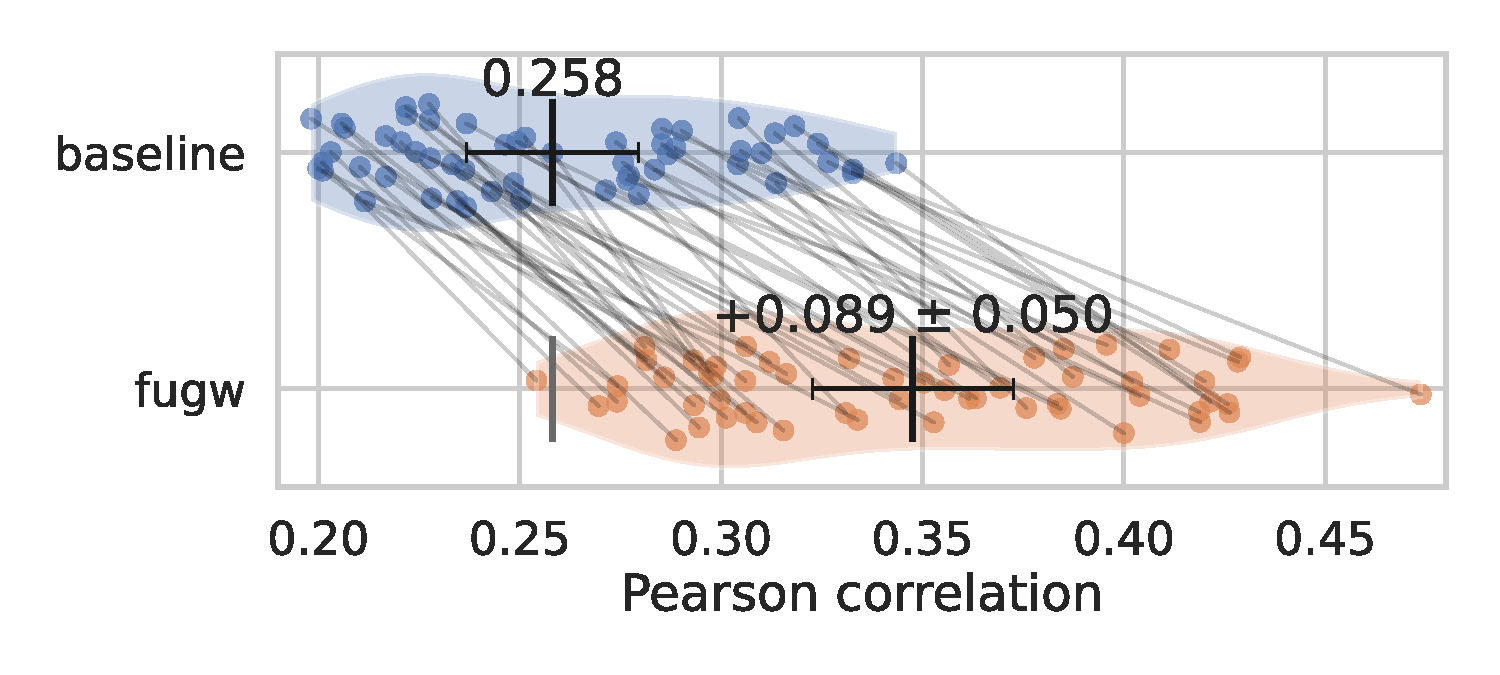
\includegraphics[width=0.5\columnwidth]{./Chapitre4/figures/individual_alignment_correlation_gain_fugw}
    \caption[Correlation between pairs of subjects is significantly better after alignment on individual anatomies than after projecting subjects onto a common anatomical template]{
        \textbf{Correlation between pairs of subjects is significantly better after alignment on individual anatomies than after projecting subjects onto a common anatomical template}
    }
    \label{fig:gain_comparisions_individual}
\end{figure}

As shown in \Cref{fig:gain_comparisions_individual},
we obtain correlation gains which are comparable to that of Experiment 1 (about 35\% gain)
while working on individual meshes.
This tends to show that FUGW can compute meaningful alignments between pairs of individuals
without the use of an anatomical template, which helps bridge most conceptual impediments listed
in \Cref{sec:introduction}.
Moreover, this opens the way for computation of simple statistics in cohorts of individuals
in the absence of a template. Indeed, one can pick an individual of the cohort and use it
as a reference subject on which to transport all other individuals.
We give an example in \Cref{fig:individual_projections},
showing that FUGW correctly preserved idiosyncrasies of each subject while
transporting their functional signal in an anatomically sound way.
\begin{figure}[H]
    \centering
    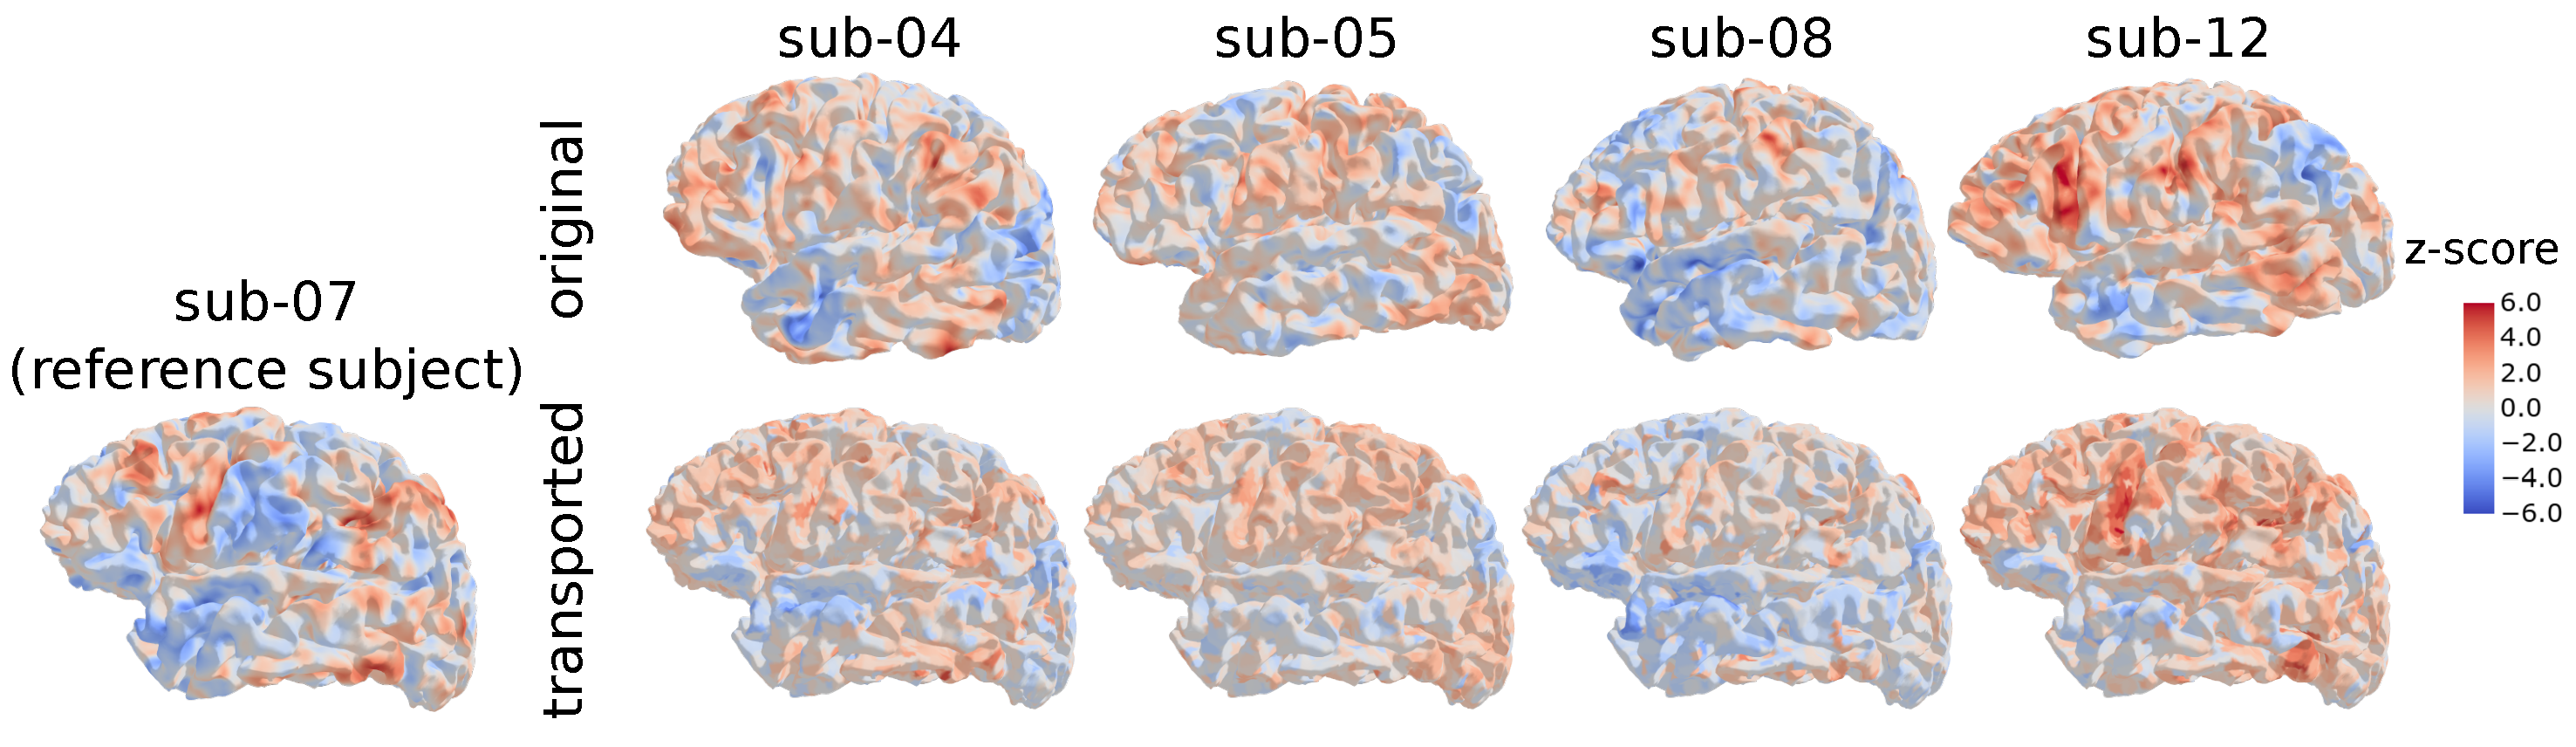
\includegraphics[width=1\columnwidth]{./Chapitre4/figures/individual_alignment.pdf}
    \caption[Transporting individual maps onto a reference subject]{
        \textbf{Transporting individual maps onto a reference subject}
        FUGW can help bridge the absence of template anatomies
        and derive pairs of alignments such that all individuals
        of the cohort are comparable. We display a map taken from the test set contrasting areas activated during mathematical reasoning against areas activated for other stimuli of the protocol.
    }
    \label{fig:individual_projections}
\end{figure}

%%%%%%%%%%%%%%%%%%%%%%%%%%%%%%%%%%%%%%%%%
\subsection{Experiment 3 - Barycenter}

In the absence of a proper metric to quantify the correctness of a barycenter,
we first qualitatively compare the functional templates obtained with and without alignment.
In \Cref{fig:barycenter_vs_group_average}.A, we do so using brain maps taken from the test set.
We can see that the barycenter obtained with FUGW yields sharper contrasts and
more fine-grained details than the barycenter obtained by per-vertex averaging.
We also display in \Cref{fig:barycenter_vs_group_average}.B
the result of a one-sample test for the same contrast, which can readily be used for inference.
The one-sample test map obtained after alignment to the FUGW template exhibits
the same supra-threshold clusters as the original approach, but also some additional spots
which were likely lost due to inter-subject variability in the \emph{fsaverage5} space.
This approach is thus very useful to increase power in group inference.
We quantify this result by counting the number of supra-threshold vertices
with and without alignment for each contrast map of the test set.
Our alignment method significantly finds more such vertices of interest,
as shown in \Cref{fig:barycenter_vs_group_average}.C.
\begin{figure}[t]
    \centering
    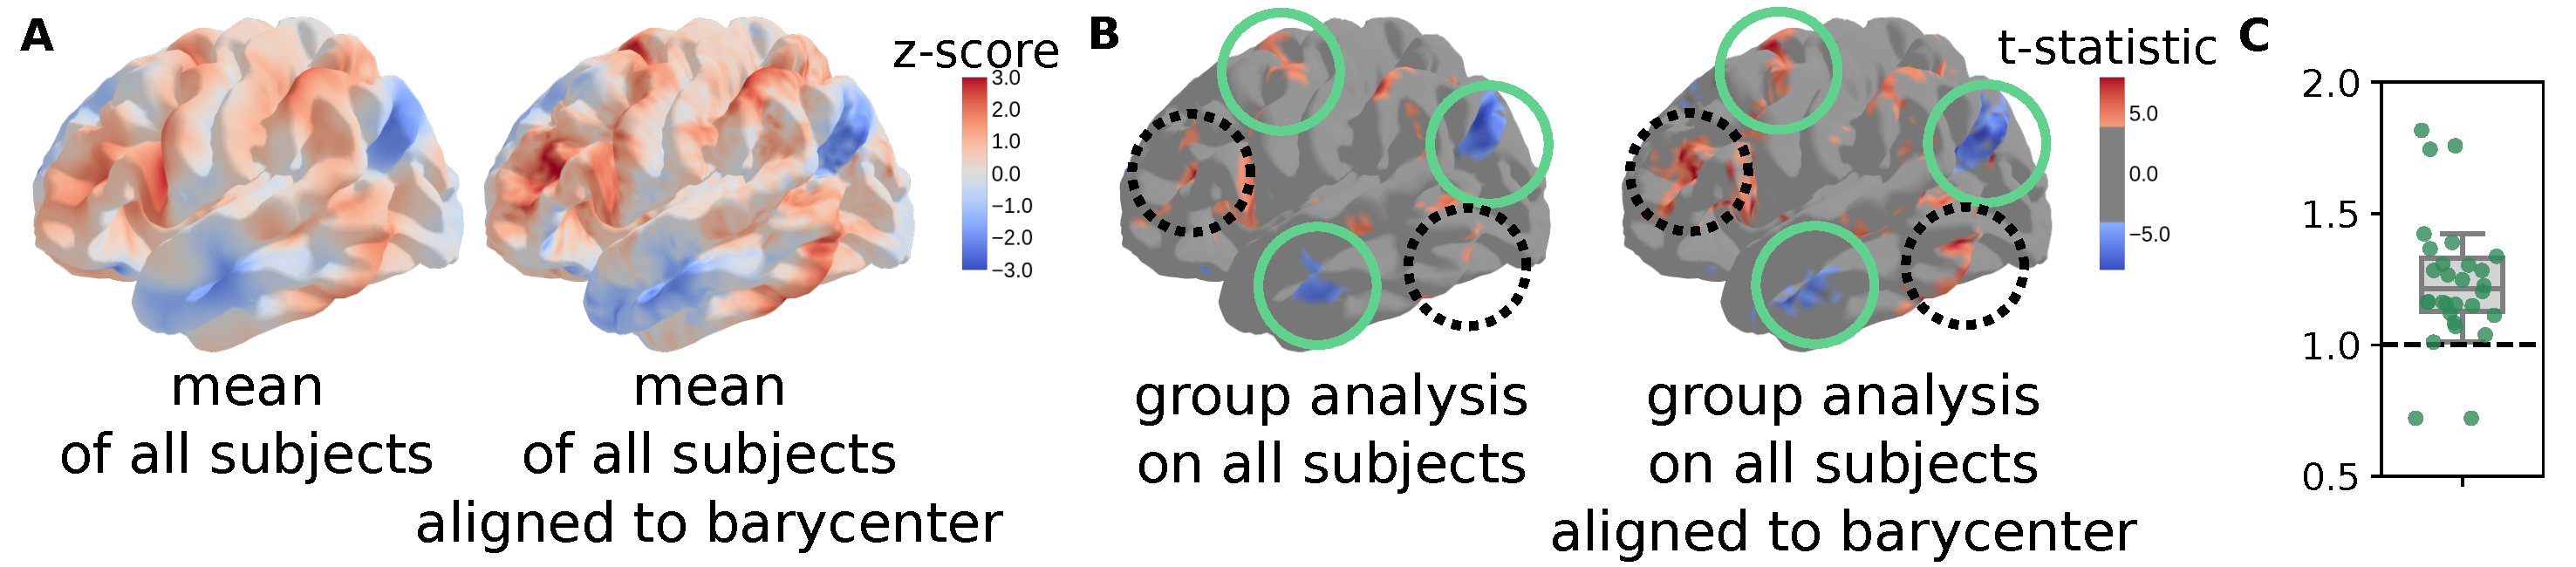
\includegraphics[width=1\columnwidth]{./Chapitre4/figures/barycenter_group_analysis.pdf}
    \caption[FUGW barycenter yields much finer-grained maps than group averages]{
        \textbf{FUGW barycenter yields much finer-grained maps than group averages}
        We study the same statistical map as in \Cref{fig:intro}, which contrasts
        areas of the brain involved in mathematical reasoning.
        \textbf{A}. These complex maps projected onto the barycenter and averaged
        show more specific activation patterns than simple group averages,
        especially in cortical areas exhibiting more variability, such as the prefrontal cortex.
        \textbf{B}. Deriving a t-test on aligned maps captures the same clusters
        as the classical approach (plain green circles), but also new clusters in areas
        where inter-subject variability is high (dotted black circles).
        Peak t-statistics are also higher with FUGW.
        \textbf{C}. Ratio of number of activated vertices ($|\text{t-statistic}| \geq 4$)
        with versus without alignment for each map of the test set.
        Our method finds significantly more of such vertices ($\text{p-value} = 3\cdot10^{-4}$).}
    \label{fig:barycenter_vs_group_average}
\end{figure}

\section{Discussion}

FUGW can derive meaningful couplings between pairs of subjects without
the need of a pre-existing anatomical template. It is well-suited to computing
barycenters of individuals, even for small cohorts.

In addition, we have shown clear evidence that FUGW yields gains that cannot be achieved
by traditional diffeomorphic registration methods.
These methods impose very strong constraints to the displacement field,
that may prevent reaching optimal configurations.
More deeply, this finding suggests that brain comparison ultimately requires
lifting hard regularity constraints on the alignment models,
and that two human brains differ by more than a simple continuous surface deformation.
However, current results have not shown a strong correlation gain of
unbalanced OT compared to balanced OT, likely because the cohort under study is too small.
Leveraging datasets such as HCP \citep{hcpdata} with a larger number of subjects
will help lower the standard error on correlation gain estimates.
In this work, we decided to rely on a predefined anatomical template (\emph{fsaverage5})
to derive functional barycenters.
It would be interesting to investigate whether more representative anatomical templates
can be learned during the process.
This would in particular help to customize templates to different populations or species.

Additionally, using an entropic solver introduces a new hyper-parameter $\varepsilon$
that has a strong effect, but is hard to interpret.
Future work may replace the Sinkhorn algorithm \citep{Sejourne19}
used here by the majorization-minimization one \citep{Chapel20},
which does not require entropic smoothing. This solution can yield sparse couplings
while being orders of magnitude faster, which will prove useful when computing barycenters
on large cohorts.

Finally, we plan to make use of FUGW to derive alignments between human and
non-human primates without anatomical priors. Indeed, the understanding of given brain mechanisms
will benefit from more detailed invasive measurements made on other species \emph{only if}
brains can be matched across species; moreover, this  raises the question of features
that make the human brain unique, by identifying patterns that have no counterpart in other species.
By maximizing the functional alignment between areas, but also allowing for some regions
to be massively shrunk or downright absent in one species relative to the other,
the present tool could shed an objective light on the important issue of whether
and how the language-related areas of the human cortical sheet map onto
the architecture of non-human primate brains.

\vfill

\chapter[Breaking isometric ties and introducing priors in Gromov-Wasserstein distance]{Breaking isometric ties and introducing priors in Gromov-Wasserstein distance}
\label{chap:agw}

\renewcommand{\contentsname}{Contents}
\localtableofcontents*
\chaptermark{\textbf{Breaking isometric ties and introducing priors in Gromov-Wasserstein distance}}

\hfill \break

\raggedbottom

This chapter presents the results from \citep{Demetci23} and address the problem of
incorporating priors into Gromov-Wasserstein (GW) distance.
GW distance has many applications in machine learning due to its ability
to compare measures across metric spaces and its invariance to isometric transformations. However,
in certain applications, this invariance property can be too flexible, thus undesirable. Moreover,
the GW distance solely considers pairwise sample similarities in input datasets,
disregarding the raw feature representations. We propose a new optimal transport formulation,
called Augmented Gromov-Wasserstein (AGW), that allows for some control over the
level of rigidity to transformations. It also incorporates feature alignments,
enabling us to better leverage prior knowledge on the input data for improved performance.
We present theoretical insights into the proposed method. We then demonstrate its usefulness
for single-cell multi-omic alignment tasks and heterogeneous domain adaptation in machine learning.

% \paragraph{Contributions} PD, IR and RS designed and planned the study. All authors wrote
% the paper and revised the manuscript. by PD and RS did the experimental design and analysis.
% The theoretical analysis of the proposed method is performed by QHT and revised by IR.

\raggedbottom

%%%%%%%%%%%%%%%%%%%%%%%%%
\section{Introduction}

Optimal transport (OT) theory provides a fundamental tool for comparing and
aligning probability measures omnipresent in machine learning (ML) tasks.
Following the least effort principle, OT and its associated metrics offer
many attractive properties that other divergences, such as the popular Kullback-Leibler or
Jensen-Shannon divergences, lack. For instance, OT borrows key geometric properties of
the underlying ``ground'' space on which the distributions are defined \citep{Villani03}
and enjoys non-vanishing gradients when measures have disjoint support \citep{Arjovsky17}.
OT theory has also been extended to a much more challenging case of probability measures supported
on different metric-measure spaces. In this scenario, the Gromov-Wasserstein (GW) distance
seeks an optimal matching between points in the supports of the considered distributions
that will minimize the distortion of intra-domain distances upon such matching.

Since its proposal by \citet{Memoli11} and further extensions by \citet{Peyre16},
GW has been successfully used in a wide range of applications, including
domain adaptation \citep{Yan18}, computational biology
\citep{Nitzan2019,Pamona,UniPort,SpaOTsc,Demetci20,Demetci22,PASTE},
generative modeling \citep{Bunne19}, and reinforcement learning \citep{GW-VAE}.

\paragraph{Limitations of prior work} Successful applications of GW distance are often
attributed to its invariance to distance-preserving transformations (also called ``isometries'')
of the input domains. Since GW considers only intra-domain distances, it is naturally invariant
to any transformation that does not alter them. While this is a blessing in many applications,
for example, comparing graphs with the unknown ordering of nodes, it may become a curse
when one has to choose the ``right'' isometry among many that yield the same GW distance.
How could one break such ties while keeping the attractive properties of the GW distance?
This question remains to be addressed in the field.

Additionally, GW distances are often used in tasks where one may have some
\textit{a priori} knowledge about the mapping between the two considered spaces.
For example, in single-cell applications, mapping a group of cells in similar tissues
across species helps understand the evolutionarily conserved and diverging cell types
and functions \citep{kriebel2022uinmf}. When performed using OT, this cross-species cell mapping
may benefit from the knowledge about an overlapping set of orthologous genes
\footnote {Genes in two different species that originated from a common ancestor and
largely maintained their function and sequence during speciation}.
GW formulation does not offer any straightforward way to incorporate this knowledge,
which may lead to suboptimal performance.

\paragraph{Our contributions}
In this chapter, we introduce a new OT formulation that addresses the drawbacks of the
GW distance mentioned above. We summarize our contributions as follows:
\begin{enumerate}
    \item We propose Augmented Gromov-Wasserstein (AGW), a new formulation that leverages
    both pairwise sample similarities in input datasets and their raw data representations;
    \item We demonstrate that AGW allows for better control over the isometric transformations
    of the GW distance and helps break isometric ties;
    \item We show that AGW can incorporate prior knowledge to guide how the two metric spaces
    should be compared, which improves object comparisons; %object matchings; Priors can also be set to further tighten isometric invariances
    \item We provide a theoretical analysis of the properties of the proposed formulation
    and examples that concretely illustrate its unique features;
    \item Our empirical results show that AGW outperforms previously proposed
    cross-domain OT methods in several downstream tasks and tends to converge in fewer iterations
    than GW. We first focus on real-world applications in computational biology,
    namely the single-cell data integration tasks. Then, we also illustrate its generalizability
    to the heterogeneous domain adaptation in ML.
    %\item runtime
\end{enumerate}
% The paper is organized as follows. Section 2 presents key notions from the OT theory
% utilized in the rest of the paper. Section 3 presents our proposed AGW formulation and
% analyzes its theoretical properties. In Section 4, we present several empirical studies
% for the single-cell alignment task and demonstrate the applicability of our method to
% the heterogeneous domain adaptation task. We conclude our paper in Section 5 with
% a discussion of potential future work.

% \paragraph{Notations} In what follows, we denote by
% $\Sigma_{n}=\{ p \in \bbR_{> 0}^n: \sum_{i=1}^{n} p_{i}=1\}$
% the simplex histogram with $n$ bins. We use $\otimes$ for tensor-matrix multiplication,
% \ie, $L \otimes B$ is the matrix $(\sum_{k,l} L_{ijkl} B_{kl})_{i,j}$ for a $4$D-tensor $L$ and
% a matrix $B$. We use $\langle \cdot, \cdot \rangle$ for the matrix scalar product associated with
% the Frobenius norm $\|\cdot\|_{F}$. We write $1_d \in \bbR^d$ for a
% $d$-dimensional vector of ones. We use the terms ``coupling matrix'', ``transport plan''
% and ``correspondence matrix'' interchangeably.
% A point in the space can also be called ``an example'' or ``a sample''.
% Given an integer $n \geq 1$, denote $[n] := \{ 1, ..., n\}$.

%%%%%%%%%%%%%%%%%%%%%%%%%%%%%%%%%%%%%%%%%%%%%%%
\section{Augmented Gromov-Wasserstein}

\begin{figure}[t]
\centering
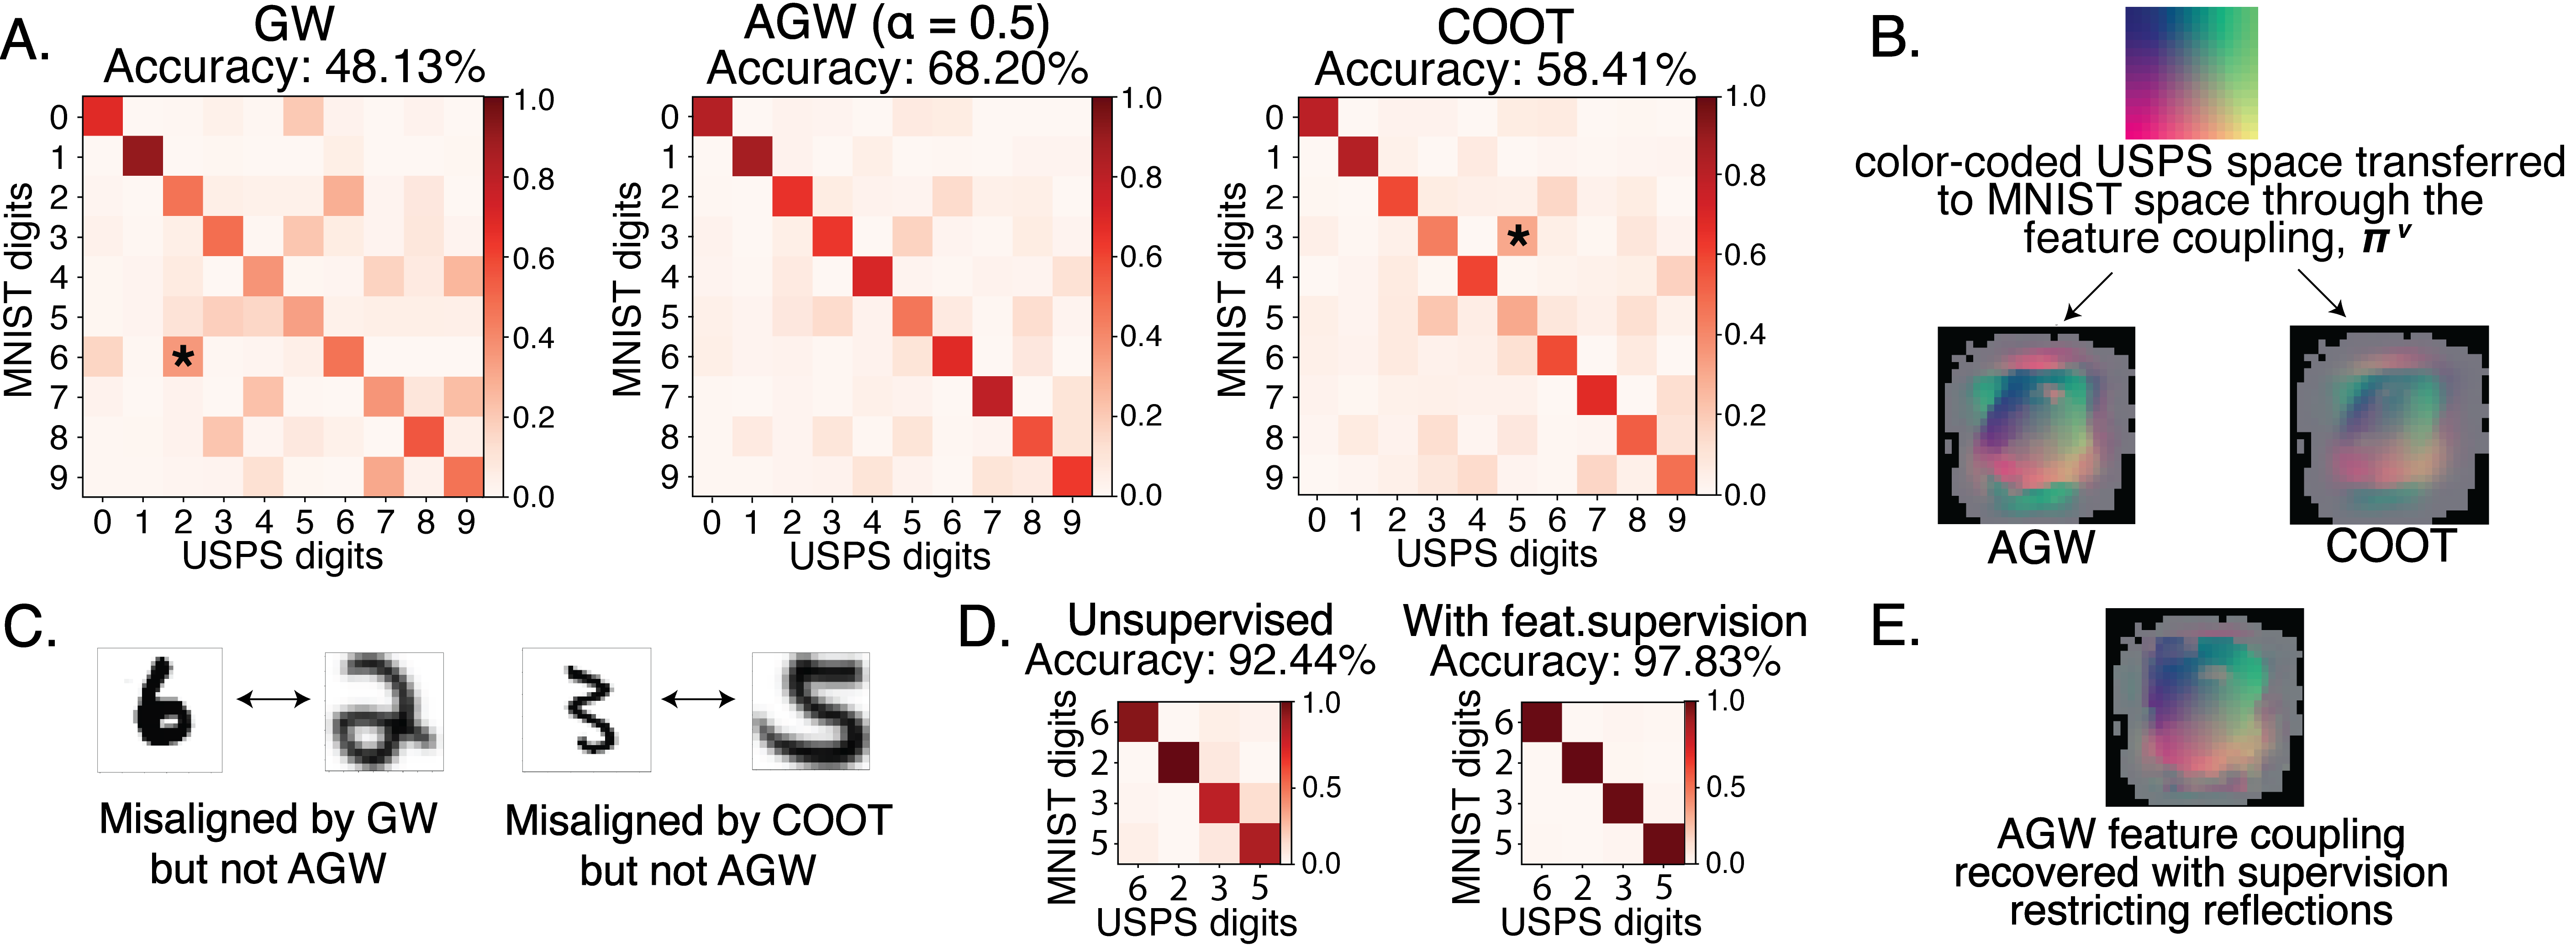
\includegraphics[width=\linewidth]{./Chapitre5/fig//mnist1_supervised.png}
\caption[Aligning digits from MNIST and USPS datasets]{Aligning digits from MNIST and USPS datasets. \textbf{(A)}
Confusion matrices of GW, AGW with $\alpha=0.5$ and COOT.
(*) denote pair alignments ;
\textbf{(B)} Feature coupling $Q$ of AGW compared to COOT;
\textbf{(C)} Illustration of a case from where GW's and COOT's invariances are
detrimental for obtaining a meaningful comparison, while AGW remains informative.
\textbf{(D)} Example showing improved digit alignment with feature-level supervision
that restricts reflections \textbf{(E)} Feature coupling recovered by AGW ($\alpha =0.5$)
in the supervised setting of (D).}
\label{fig:mnist}
\end{figure}

Here, we start by outlining the motivation for our proposed formulation,
highlighting the different properties of GW distance and COOT. Then,
we detail our AGW distance that interpolates between the two, followed by a
theoretical study of its properties.

\subsection{Motivation}

\paragraph{Invariances of GW} GW distance remains unchanged under isometric transformations of
the input data. This property has contributed much to the popularity of GW distance,
as isometries naturally appear in many applications. However,
not all isometries are equally desirable. For instance, a rotation of the
handwritten digit $6$ seen as a discrete measure can lead to its slight variation
for small angles or to a digit $9$ when the angle is close to $180$ degrees. In both cases,
however, the GW distance remains unchanged, making it insufficient to distinguish
the two digits apart.

\paragraph{Invariances of COOT} Unlike GW, COOT has fewer degrees of freedom
in terms of invariance to global isometric transformations as it is limited to
permutations of rows and columns of the two matrices, and not all isometric transformations
can be achieved via such permutations.

Additionally, COOT is strictly positive for any two datasets of different sizes either
in terms of features or samples, making it much more restrictive than GW.
It thus provides a fine-grained control when comparing complex objects,
yet it lacks the robustness of GW to frequently encountered transformations
between the two datasets. Further, unlike GW, it is invariant to local isometries
that can be achieved via permutations of a subset of features.

\subsection{AGW formulation} \label{subsec:agw_formulation}
Given the above discussion on the invariances of COOT and GW distance,
interpolating between them will restrict each other's invariances. Additionally,
interpolating with COOT is a natural way to introduce raw feature alignments in GW,
which allows for leveraging priors on them. We call this interpolation \textbf{Augmented GW} (AGW).
Recall that a weighted matrix is the triplet $\cX = (X, \mu_1^X, \mu_2^X)$, where
$X \in \bbR^{n_x \times d_x}, \mu_1^X \in \Delta_{n_x}$ and $\mu_2^X \in \Delta_{d_x}$.
Given $\alpha \in [0,1]$, we define the AGW between two weighted matrices $\cX$ and $\cY$ as
\begin{align}
\label{eq:scootr}
\agw_{\alpha}(\cX, \cY) &:=
\min_{\substack{P \in U(\mu_1^X, \mu_1^Y) \\ Q \in U(\mu_2^X,\mu_2^Y)}} \quad
\alpha \; \langle L(C^x,C^y) \otimes P, P \rangle + (1-\alpha) \; \langle L(X,Y) \otimes P, Q \rangle,
\end{align}
where, for $p \geq 1$,
\begin{itemize}
    \item[$\bullet$] $\langle L(C^x,C^y) \otimes P, P \rangle
    = \sum_{i,j,k,l} \; (C^x_{ik} - C^y_{jl})^p P_{ij} P_{kl}$ is the objective function of
    the GW distance. Here, the matrices $C^x \in \bbR^{n_x \times n_x}$ and
    $C^y \in \bbR^{n_y \times n_y}$
    contain the intra-domain pairwise distances between the rows of $X$ and $Y$, respectively.
    More precisely, the distance matrices are of the form:
    $C^x_{ik} = ||x_i - x_k||_q$ and $C^y_{jl} = ||y_j - y_l||_q$, for some $q > 0$. Here,
    $(x_i, x_k) \in \bbR^{d_x} \times \bbR^{d_x}$ and $(y_j, y_l) \in \bbR^{d_y} \times \bbR^{d_y}$
    are tuples of rows in $X$ and $Y$, respectively.

    \item[$\bullet$] $\langle L(X,Y) \otimes P, Q \rangle =
    \sum_{i,j,k,l} \; (X_{ik} - Y_{jl})^p P_{ij} Q_{kl}$ is the objective function of the COOT.
\end{itemize}
The AGW problem always admits a solution. Indeed, as the objective function is continuous
and the sets of admissible couplings are compact, the existence of minimum and minimizer
is guaranteed. In practice, we mostly consider $p=2$ for computational convenience.

When $\alpha = 1$, we recover the GW distance, whereas $\alpha = 0$ corresponds to the
COOT. Our interpolation offers several important benefits. First, COOT term ensures that AGW
will take different values for any two isometries whenever the dimensions are different: $d_x \neq d_y$. Intuitively,
AGW's value will then depend on how ``far'' a given isometry is from a permutation of rows
and columns of the inputs. Thus, we restrict a broad class of (infinitely many) transformations
that GW cannot distinguish and we tell them apart by assessing whether they
can be approximately obtained by simply swapping 1D elements in input matrices.

Second, combining the objective functions of COOT and GW distance allows us to
effectively influence the optimization of $P$ by introducing priors on feature matchings
through $Q$ and vice versa. This can be achieved by penalizing the costs of matching
certain features in the COOT term to influence the optimization of $Q$. This prior knowledge
guides how the two metric spaces should be compared and improves empirical performance.
These key properties explain our choice of calling it ``augmented'':
we equip GW distance with an ability to provide finer-grained object comparisons by
breaking isometric ties and/or guiding the matching using available prior knowledge.

\paragraph{Illustrations} We illustrate AGW's properties on a task of aligning handwritten digits
from MNIST \citep{lecun10} (28$\times$28 pixels) and USPS datasets (16$\times$16 pixels)
\citep{Hull94} in \Cref{fig:mnist}, where AGW with $\alpha=0.5$ outperforms both GW and COOT
in alignment accuracy (Panel A). The black asterisks show the digit pairs that most benefit
from AGW interpolation, which are $6-2$ for GW and $3-5$ for COOT.
Panel C visualizes examples from these digit pairs that are misaligned by GW and COOT
but not by AGW.
\footnote{Here, we define ``aligned pairs'' as pairs of digits with the
highest coupling probabilities.}. Here, we observe that 6-2 misalignment by GW is likely because
one is a close reflection of the other across the y-axis. Similarly,
COOT mismatches 3 and 5 as one can obtain 3 from 5 by a local permutation of
the upper half of the pixels. Panel B visualizes the feature couplings obtained by
AGW (on the left) and COOT (on the right). The feature coupling by COOT confirms that
COOT allows for a reflection across the y-axis on the upper half of the image
but not on the lower half. With AGW, both of these misalignments improve,
likely because (1) the correct feature alignments in the lower half of the images
prevent 6 and 2 from being matched and (2) GW distance is non-zero for 5-3 matches
since the transformation is not applied to the whole image. In Panels D and E,
we also show that providing supervision on feature alignments to restrict local reflections
further improves AGW's performance.

Similar improvement can be seen for aligning cells (samples) for two different single-cell
measurements (features) \citep{SNAREseq} in Figure S2. Panel A shows that AGW consistently maps
the 4 cell types in the data better than GW (a popular method for this task
\citep{Pamona,Demetci20,Demetci22,UniPort}) over 50 random subsampling of cells.
The 2D projection of alignments in Panel B shows that GW sometimes completely swaps
the cell type clusters when they have a similar number of cells, whereas AGW is more robust
to this phenomenon.

\paragraph{Optimization} For simplicity, suppose $n_x = n_y = n$ and $d_x = d_y = d$.
With the squared loss in both GW and COOT terms (meaning that $p=2$),
the computational trick by \citet{Peyre16}
can be applied, which reduces the complexity of AGW from $O(n^4 + n^2 d^2)$
to $O(n^3 + dn^2 + nd^2)$. For optimization, we use the block coordinate descent (BCD) algorithm,
where we alternatively fix one coupling and minimize AGW with respect to the other (\Cref{alg:bcd_agw}).
Each iteration then consists of solving two OT problems. To further accelerate the optimization,
entropic regularization \citep{Cuturi13} can be used on either $P$, $Q$, or both.
In practice, we rely on the built-in functions of the Python Optimal Transport package \citep{Flamary21}.

\begin{algorithm}[t]
    \caption{BCD algorithm to solve AGW \label{alg:bcd_agw}}
    \begin{algorithmic}[1]
      \STATE Initialize $P^*$ and $Q^*$.
      \REPEAT
      \STATE Calculate $L_Q = L(X, Y) \otimes P^*$.
      \STATE For fixed $P$, solve the OT problem:
      $Q^* \in \argmin_{Q \in U(\mu_2^X, \mu_2^Y)} \langle L_Q, Q \rangle$.
      \STATE Calculate $L_P = L(X, Y) \otimes Q^*$.
      \STATE For fixed $Q$, solve the fused GW problem:
      \begin{align}
        P^* \in \argmin_{P \in U(\mu_1^X, \mu_1^Y)}
        \alpha \; \langle L(D_X,D_Y) \otimes P, P \rangle + (1-\alpha) \langle L_P, P \rangle.
      \end{align}
      \UNTIL{convergence}
\end{algorithmic}
\end{algorithm}

%%%%%%%%%%%%%%%%%%%%%%%%%%%%%%%%%%%%%%%%%%%%%%
\subsection{Theoretical analysis} \label{subsec:agw_property}

Intuitively, we expect that AGW interpolates between GW and COOT.
The following result formalizes this observation.
\begin{proposition}
\label{prop:basic_prop}
Given two weighted matrices $\cX$ and $\cY$, when $\alpha \to 0$ (or $1$),
one has $\agw_{\alpha}(\cX, \cY) \to \coot(\cX, \cY)$ (or $\gw(\cX, \cY)$).
\end{proposition}
We also expect that AGW inherits the metric properties from GW and COOT distances.
\begin{proposition}[Metric properties]
    \label{prop:metric_agw}
    For $\alpha \in [0, 1]$, AGW satisfies the triangle inequality. Moreover,
    suppose that $\mu_1^X, \mu_1^Y, \mu_2^X, \mu_2^Y$ are uniform distributions. Then for
    $\alpha \in [0, 1)$, AGW defines a distance on the space of weighted matrices,
    up to permutation of the matrix coordinates. More precisely, $Y$ is
    obtained by permuting entries of $X$ if and only if $\agw_{\alpha}(\cX, \cY) = 0$.
\end{proposition}
In other words, $\agw_{\alpha}(\cX, \cY) = 0$ if and only if $\coot(\cX, \cY) = 0$.
Under mild conditions, we can further characterize the isometries encoded by AGW.
First, let us denote $\cO_d$ and $\cP_d$ the sets of orthogonal and permutation matrices of size $d$,
respectively. Given a matrix $X \in \bbR^{n \times d}$, we assume that
\begin{assumption}
    \label{assumption:1}
    $X$ is full-rank and has exactly $\min(n, d)$ distinct singular values.
\end{assumption}
The full-rank assumption is not uncommon in the machine learning literature \citep{Kenji19}
and can be easily met in practice. Additionally,
not only the Hermitian matrices with repeated eigenvalues are rare (see page 56 in \citep{Tao12}),
but we can even show that
\begin{corollary}
\label{corr:hermitian}
    The set of Hermitian matrices with repeated eigenvalues has zero Lebesgue measure.
\end{corollary}
Since the singular values of $X$ are determined by the symmetric matrix $X X^T$,
\Cref{corr:hermitian} assures that it is reasonable to exclude all symmetric matrices
with repeated eigenvalues. With these, we present:
\begin{theorem}
\label{thm:invariant}
Given two weighted matrices $\cX$ and $\cY$. Suppose $X \in \bbR^{n \times d}$,
where $n \geq d$, satisfies \Cref{assumption:1}.
For any $0 < \alpha < 1$, if $\agw_{\alpha}(\cX, \cY) = 0$,
then there exist a symmetric orthogonal matrix $O \in \cO_d$ and
a permutation matrix $P \in \cP_d$ such that $Y = X OP$.
\end{theorem}
% Despite the simplicity of the interpolation structure, the invariances induced by AGW
% present novel and non-trivial challenges for theoretical analysis.
% While sharing basic invariances, such as feature swaps, AGW covers much fewer isometries than
% GW distance.
% Given the superior empirical performance of AGW over GW and COOT, such isometries appear
% meaningful and relevant in real-world tasks.

\paragraph{Weak invariance to translation}
While enjoying the interpolation and metric properties, AGW does not inherit the invariance
to the translation of the GW distance. However, we find that it satisfies a relaxed version
of this invariance defined as follows.
\begin{definition}
    We call $D = \inf_{\pi \in \cU} F(\pi, X, Y)$, where $X, Y$ are input data and $\cU$
    is a set of feasible couplings and $F$ is a real-valued functional, an OT-based divergence.
    Then $D$ is weakly invariant to translation if for every $a, b \in \bbR$, we have
    $\inf_{\pi \in U} F(\pi, X + a, Y+b) = \inf_{\pi \in \cU} F(\pi, X, Y) + c$,
    for some constant $C$ depending on $a, b, X, Y$ and $\cU$.
\end{definition}
Here, we denote the translation of $X$ as $X + a$, whose elements are of the form $X_{ij} + a$.
Intuitively, an OT-based divergence is weakly invariant to translation if only
the optimal transport plan is preserved under translation, but not necessarily the divergence itself.
In practice, we would argue that the ability to preserve the optimal plan under translation
is much more important than preserving the distance itself. In other words,
the translation only shifts the divergence by a constant but has no impact on the optimization procedure,
meaning that the OT plan remains unchanged. This is indeed the case of AGW.
\begin{proposition}
    \label{prop:invariant} For $p=2$ and for any $\alpha \in [0,1]$,
    AGW is weakly invariant to translation.
\end{proposition}

%%%%%%%%%%%%%%%%%%%%%%%%%%%%%ù
\subsection{Related work}

Most related to our work is the Fused Gromov-Wasserstein (FGW) distance \citep{Vayer19b}
that compares structured objects. Its objective function is a convex combination of
the GW term defined based on the pairwise intra-domain distances and the Wasserstein term
defined over additional features that live in the same space for both input matrices.
Despite the resemblance to FGW, AGW fundamentally differs from it in several ways.
Firstly, AGW uses explicit control over the invariances of GW to provide more meaningful
cross-domain matchings. No other OT-based metric in the literature (including FGW)
leverages a similar idea.

Secondly, FGW is mostly used for structured objects endowed with additional information living
in the same space, for example, two graphs where each node may be colored by
a specific color (``additional'' feature). On the other hand, AGW can be used on
empirical measures defined for any set of objects across domains, including ones
from different dimensional spaces, and requires no additional information.

Finally, the notion of feature space in FGW does not have the same meaning as in AGW.
The feature space in FGW is associated with the sample space, whereas in AGW (and also in COOT),
the two spaces are independent. Each element of the former is
associated with a point in the sample space. By contrast, the features in AGW are
precisely the coordinates of a point, in addition to its representation in the
original and dissimilarity-induced spaces.

%%%%%%%%%%%%%%%%%%%%%%%%%%%%%%%%%%%%%%%%
\section{Experimental evaluations}

\begin{table}[t]
\begin{center}
\resizebox{1.0\linewidth}{!}{
\begin{tabular}{lccccccc}
\hline
                                     & \textbf{Simulation 1}                                           & \textbf{Simulation 2}                                          & \textbf{Simulation 3}                                          & \textbf{Simulated RNA-seq}      & \textbf{scGEM}                                              & \textbf{SNARE-seq}                                                & \textbf{CITE-seq}                                             \\
                                     & \begin{tabular}[c]{@{}c@{}}(300x1000, \\ 300x2000)\end{tabular} & \begin{tabular}[c]{@{}c@{}}(300x1000,\\ 300x2000)\end{tabular} & \begin{tabular}[c]{@{}c@{}}(300x1000,\\ 300x2000)\end{tabular} & \begin{tabular}[c]{@{}c@{}}(5000x50, \\ 5000x500)\end{tabular}                 & \begin{tabular}[c]{@{}c@{}}(177x28,\\  177x34)\end{tabular} & \begin{tabular}[c]{@{}c@{}}(1047x1000,\\  1047x3000)\end{tabular} & \begin{tabular}[c]{@{}c@{}}(1000x25, \\ 1000x24)\end{tabular} \\ \hline
\multicolumn{1}{l|}{\textbf{AGW}}    & \textbf{0.0730}                                                 & \textbf{0.0041}                                                & \textbf{0.0082}                                                & \textbf{0.0}                                                                   & 0.183                                                       & \textbf{0.132}                                                    & \textbf{0.091}                                                \\
\multicolumn{1}{l|}{\textbf{GW}}     & 0.0866                                                          & 0.0216                                                         & {\underline{0.0084}}                                                   & 7.1e-5                                                                         & 0.198                                                       & 0.150                                                             & 0.121                                                         \\
\multicolumn{1}{l|}{\textbf{COOT}}   & {\underline{0.0752}}                                                    & \textbf{0.0041}                                                & 0.0088                                                         & \textbf{0.0}                                                                   & 0.206                                                       & 0.153                                                             & 0.132                                                         \\
\multicolumn{1}{l|}{\textbf{UGW}}    & 0.0838                                                          & 0.0522                                                         & 0.0105                                                         & 0.096                                                                          & \textbf{0.161}                                              & {\underline{0.140}}                                                       & {\underline{0.116}}                                                   \\
\multicolumn{1}{l|}{\textbf{UCOOT}}  & 0.0850                                                          & {\underline{0.0081}}                                                   & 0.0122                                                         & 0.115                                                                          & {\underline{0.181}}                                                 & 0.188                                                             & 0.127                                                         \\
\multicolumn{1}{l|}{\textbf{bindSC}} & N/A                                                             & N/A                                                            & N/A                                                            & 3.8e-4                                                                         & N/A                                                         & 0.242                                                             & 0.144                                                         \\ \hline
\end{tabular}}
\end{center}
\caption{\label{table:scCells} \textbf{Single-cell alignment error},
as quantified by the average `fraction of samples closer than true match'
(FOSCTTM) metric (lower values are better).
For each dataset, the size of the two domains they contain are expression in the format
(number of samples x number of features) in the second row.
}
\end{table}

We apply AGW to the single-cell multi-omics alignment and heterogeneous domain adaptation tasks.
Overall, we aim to empirically answer:
\textbf{(1)} Does tightening invariances improve upon GW's performance in tasks where
it has been previously used? \textbf{(2)} Does prior knowledge introduced in AGW help
in obtaining better cross-domain matchings?

\paragraph{Baselines} We pick other cross-domain OT methods as baselines, namely COOT, GW,
and their unbalanced counterparts, UCOOT \citep{Tran23} and UGW \citep{Sejourne20}.
Note that we leave extending AGW to unbalanced scenarios for future work.
We consider entropic regularization for all methods on both sample and
(when applicable) feature couplings. We keep the hyperparameter values considered
for all regularization coefficients consistent across all methods. We report the results of
the best-performing hyperparameter combination after tuning on a validation set for each method
in each experiment.

\begin{figure}[t]
\centering
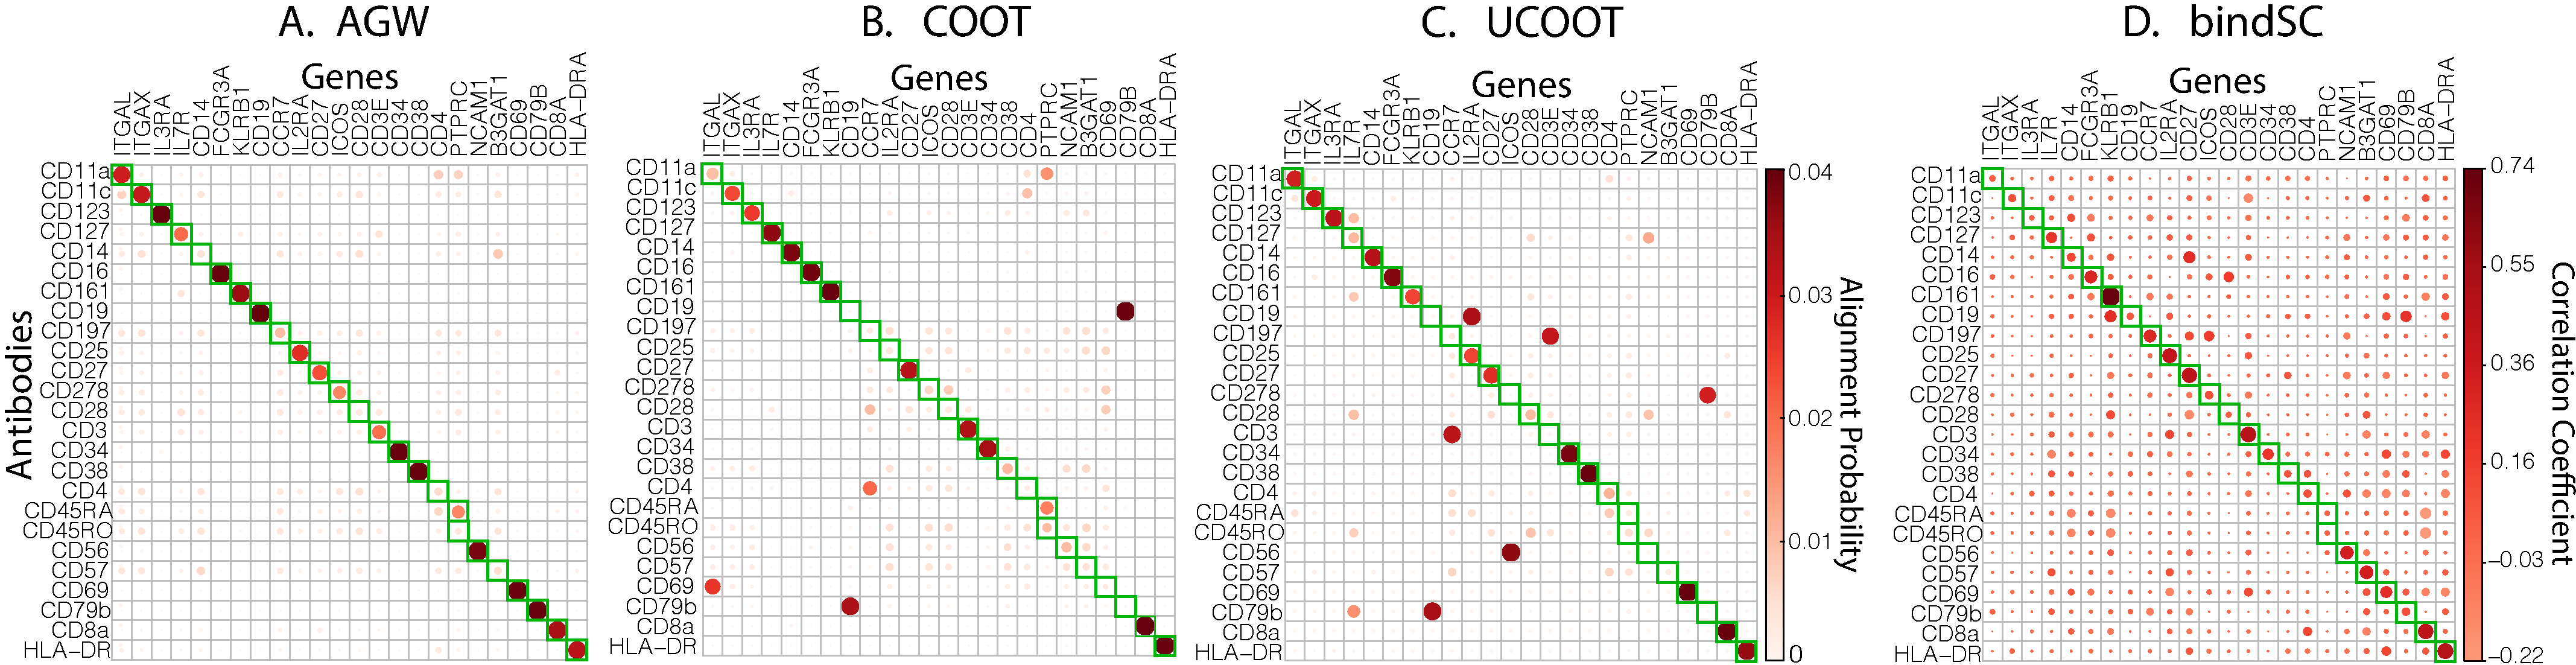
\includegraphics[width=\linewidth]{./Chapitre5/fig/cite_fgcoot_final.pdf}
\caption[Feature alignments for the CITE-seq dataset]{\label{fig:cite} Feature alignments for the CITE-seq dataset. Green boxes indicate
where we expect matches (a notion of ``ground-truth'') based on domain knowledge.}
\end{figure}

\subsection{Integrating single-cell multi-omics datasets}
Integrating data from different single-cell sequencing experiments is
an important biological task for which OT has proven useful \citep{Pamona,UniPort,Demetci20}.
Single-cell experiments measure various genomic features at the individual cell resolution.
Jointly studying these can give scientists insight into the mechanisms regulating cells.
However, experimentally combining multiple types of measurements for the same cell
is challenging for most combinations. Scientists rely on the computational integration
of multi-modal data taken on different but related cells (\eg, by cell type or tissue)
to study the relationships and interactions between different aspects of the genome.

We particularly focus on this task for two reasons. First, GW is used as a state-of-the-art
method for this task \citep{Pamona,Demetci22,UniPort}, so it is important to see if
AGW improves upon it. Second, several single-cell benchmark datasets provide
ground-truth matchings on the feature- and the sample-level alignments.
This information allows us to assess the effect of guiding cross-domain matching with partial
or full prior knowledge of these relationships.

\paragraph{Single-cell alignment} We follow the first GW application in this domain
\citep{Demetci20} and align samples (\ie, cells) of simulated and real-world datasets
from different measurement types. We have ground-truth information on cell-cell alignments
for all datasets, which we only use for benchmarking. We demonstrate in \Cref{table:scCells}
that AGW consistently yields higher quality cell alignments (with lower alignment error)
compared to the state-of-the-art baselines, including GW, COOT, and their unbalanced counterparts.

We include bindSC as an additional baseline, which performs bi-order canonical correlation analysis
to align single-cell datasets. Unlike other single-cell alignment methods,
it internally computes a feature correlation matrix that users can extract. So,
we include it as a baseline to compare its feature alignment performance against
AGW in the next section. However, bindSC usage is limited to a few measurement types
as it requires an input matrix that relates features across domains to bring the datasets
into the same space at initialization. We do not have this information for most datasets,
thus the ``N/A'' entries in \Cref{table:scCells}.

% It is important to note that an unbalanced extension could be developed for AGW through future work to potentially further boost the results.

\paragraph{Aligning genomic features} AGW augments GW formulation with a feature coupling matrix.
Therefore, we jointly align features and see whether AGW reveals relevant biological relationships.
All current single-cell alignment methods only align samples (\ie, cells),
except for bindSC as discussed above.

Among the real-world datasets in \Cref{table:scCells}, CITE-seq \citep{CITEseq}
is the only one with ground-truth information on feature correspondences.
This dataset has paired single-cell measurements on the abundance levels of
25 antibodies and activity (i.e., ``expression'') levels of genes,
including the genes that encode these 25 antibodies. So, we first present
unsupervised feature alignment results on the CITE-seq dataset.
We compare our feature alignments with bindSC, COOT, and UCOOT in \Cref{fig:cite}.
The entries in the feature alignment matrices are arranged such that
the ``ground-truth'' correspondences lie in the diagonal, marked by green squares.
While AGW correctly assigns 19 out of 25 antibodies to their encoding genes with
the highest alignment probability, this number is 16 for UCOOT, 15 for COOT and
13 for bindSC (which yields correlation coefficients instead of alignment probabilities).
Additionally, the OT methods yield more sparse alignments thanks to
the ``least effort'' requirement in their formulation.

\begin{table}[t]
\begin{center}
\resizebox{1.0\linewidth}{!}{
\begin{tabular}{@{}lccccccccc@{}}
\toprule
               & \textbf{A $\rightarrow$ A} & \textbf{A $\rightarrow$ C} & \textbf{A $\rightarrow$ W} & \textbf{C $\rightarrow$ A} & \textbf{C $\rightarrow$ C} & \textbf{C $\rightarrow$ W} & \textbf{W $\rightarrow$ A} & \textbf{W $\rightarrow$ C} & \textbf{W $\rightarrow$ W} \\ \midrule


\textbf{AGW}   & \textbf{93.1$\pm$1.6}                               & \textbf{68.3$\pm$14.1}                              & \textbf{79.8$\pm$3.5}                               & \underline{55.4$\pm$7.1}                              & \underline{76.4$\pm$5.6}                               & \textbf{57.7$\pm$14.3}                              & 60.1$\pm$9.1                               & \textbf{60.9$\pm$13.3}                              & \textbf{97.3$\pm$0.9}                               \\
\textbf{GW}    & 86.2$\pm$2.3                               & 64.1$\pm$6.2                               & \underline{77.6$\pm$11.1}                              & 53.0$\pm$13.2                              & \textbf{81.9$\pm$10.5}                              & \underline{53.5$\pm$15.9}                              & 50.4$\pm$22.1                              & 54.3$\pm$14.7                              & 92.5$\pm$2.6                               \\
\textbf{COOT}  & 50.3$\pm$15.9                              & 35.0$\pm$6.4                               & 39.8$\pm$14.5                              & 40.8$\pm$15.8                              & 33.5$\pm$10.7                              & 37.5$\pm$10.4                              & 44.3$\pm$14.0                              & 27.4$\pm$10.2                              & 57.9$\pm$13.4                              \\
\textbf{UGW}   & \underline{90.6$\pm$6.5}                             & \underline{67.2$\pm$12.7}                            & 75.4$\pm$3.1                             & \textbf{56.3$\pm$14.6}                            & 69.2$\pm$8.7                            & 51.2$\pm$13.1                           & \textbf{66.7$\pm$9.9}                             & 58.4$\pm$4.7                            & \underline{94.7$\pm$1.5}                             \\
\textbf{UCOOT} & 65.4$\pm$2.1                              & 44.6$\pm$3.8                               & 36.4$\pm$1.2                               & 55.1$\pm$8.6                               & 52.1$\pm$3.8                               & 41.8$\pm$14.9                              & \underline{63.2$\pm$4.0}                               & \underline{59.7$\pm$6.3}                               & 80.3$\pm$2.1                               \\
\bottomrule
\end{tabular}}
\end{center}
\caption{\label{tab:hda_agw}
\textbf{Heterogeneous domain adaptation results (unsupervised)}.
Best results are bolded, and second-bests are underlined. For AGW,
the $\alpha$ values used are respectively $0.6, 0.9, 0.7, 0.9, 0.3, 0.8, 0.7, 0.2, 0.6$. }
\end{table}

\paragraph{Leveraging prior knowledge}
Finally, we show the advantage of providing priors by aligning a
multi-species gene expression dataset containing measurements from
the adult mouse prefrontal cortex \citep{mouse} and pallium of bearded lizard \citep{lizard}.
Since measurements come from two different species, the feature space (i.e., genes) differs,
and there is no 1-1 correspondence between the samples (i.e., cells). However,
there is a shared subset within the features, i.e., orthologous genes that
descend from a common ancestor and maintain similar biological functions in both species.
We also have domain knowledge on cells that belong to similar cell types across the two species.
Thus, we expect AGW to recover these relationships.

\begin{figure}[t]
\centering
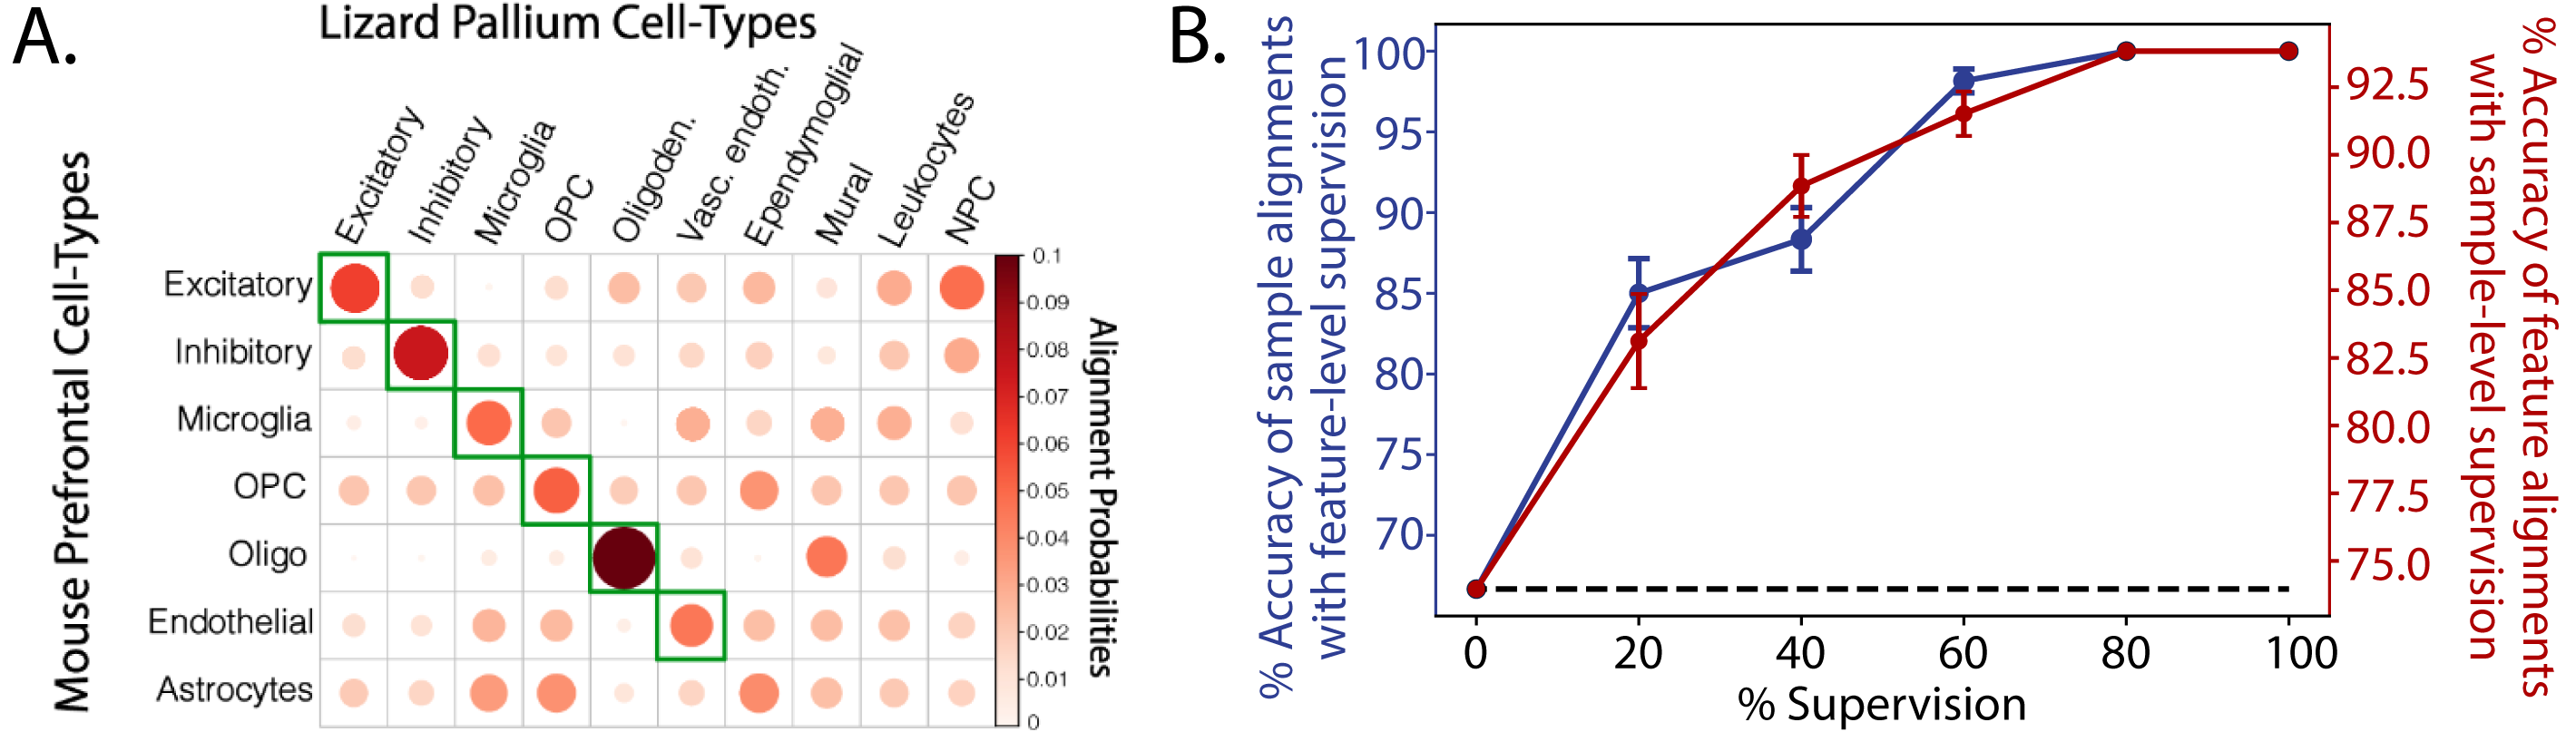
\includegraphics[width=\linewidth]{./Chapitre5/fig/xSp_full.png}
\caption[Aligning cross-species dataset]{\label{fig:xsp} \textbf{Aligning cross-species dataset.}
A. AGW's cell-type alignments.
B. Providing supervision on one level of alignment (\eg, features)
boosts alignments on the other. Standard errors computed over 10 random runs.
Dashed line indicates the sample alignment performance of GW and bindSC
(orthologous gene used in input).}
\end{figure}

\Cref{fig:xsp}A visualizes the cell-type alignment probabilities yielded by AGW
when full supervision is provided on the $10,816$ orthologous genes.
The green boxes indicate alignment between similar types of cells.
This matrix is obtained by averaging the sample alignment matrix
(\ie, cell-cell alignments) into cell-type groups. We observe that
AGW yields biologically plausible alignments, as all the six cell types that
have a natural match across the two species are correctly matched.
We also show in \Cref{fig:xsp}B that providing supervision on one alignment level (\eg,
features) improves the quality on the other alignment level (\eg, samples).

%%%%%%%%%%%%%%%%%%%%%%%%%%%%%%%%%%%%%%%%%%%%%%
\subsection{Heterogeneous domain adaptation}

Finally, we demonstrate the generalizability of our approach on a popular ML task,
heterogeneous domain adaptation, where COOT and GW were previously successfully used.
Domain adaptation (DA) refers to the problem in which a classifier learned on one domain
(called \textit{source}) can generalize to the other (called \textit{target}). Here,
we apply AGW to unsupervised and semi-supervised heterogeneous DA (HDA) tasks,
where the source and target samples live in different spaces, and we have as few as
zero labeled target samples.

\paragraph{Datasets and experimental setup}
We follow the experimental setup by \citet{Redko20} and use source-target pairs
from the Caltech-Office dataset \citep{Saenko10}. We consider all pairs between three domains:
Amazon (A), Caltech-$256$ (C), and Webcam (W), whose images are embeddings from
the second last layer in the GoogleNet \citep{Szegedy15} (vectors in $\bbR^{4096}$)
and CaffeNet \citep{Jia14} (vectors in $\bbR^{1024}$) neural network architectures.

In semi-supervised settings, we incorporate prior knowledge on a few target labels
by adding an extra cost matrix to the training of sample coupling, so that
a source sample will be penalized if it transfers mass to the target samples from different classes.
Once the sample coupling $P$ is learned, we obtain the final prediction using label propagation:
$\widehat{y}_t = \argmax_k L_{k\cdot}$,
where $L = D_s P$ and $D_s$ denotes one-hot encodings of the source labels $y_s$.

All hyperparameters are tuned on a validation set based on accuracy.
We evaluate AGW against GW and COOT on source-target pairs from the Caltech-Office dataset
\citep{Saenko10} by considering all pairs between the three domains: Amazon (A), Caltech-$256$ (C),
and Webcam (W), similarly to \citep{Redko20}. We randomly choose 20 samples per class
and perform adaptation from CaffeNet to GoogleNet and repeat it 10 times.
We report the average performance of each method along with the standard deviation.
Differently than \citep{Redko20}, we (1) unit normalize the dataset prior to alignment
as we empirically found it to boost all methods' average performance compared to using
unnormalized datasets, (2) use cosine distances when defining intra-domain distance matrices
for GW and AGW, as we found them to perform better than Euclidean distances,
and (3) report results after hyperparameter tuning methods for each pair of datasets.
Specifically, for each pair of (A)-(C), (A)-(W), etc, we sweep a hyperparameter grid over
5 runs of random sampling, choose the best-performing combination, and run
10 runs of random sampling to report results.

For all methods that allow for entropic regularization,
we consider their version with no entropic regularization (either on the sample-level alignments,
feature-level alignments, or both), along with various levels of regularization.
For entropic regularization over sample alignments, we consider
$\varepsilon_1 \in [ 5e-4, 1e-3, 5e-3, 1e-2, 5e-2, 0.1] $. For entropic regularization over
feature alignments in COOT and AGW, we consider $\varepsilon_2 \in [ 5e-4, 1e-3, 5e-3, 1e-2, 5e-2, 0.1]$.
As the interpolation coefficient of AGW, we consider $\alpha \in [ 0.1, 0.2, ..., 0.9]$.

\paragraph{Results} \Cref{tab:hda_agw} presents the performance of each method averaged across
ten runs in the unsupervised setting, where AGW yields favorable results in 6 out of 9 cases.
In two cases, UGW, and in one case, UCOOT, outperform AGW despite the lower performance of
their balanced counterparts. In these cases, unbalanced formulations prove beneficial,
and support extending AGW to unbalanced scenarios as future work.

\section{Discussion}

We present Augmented Gromov-Wasserstein (AGW), a new OT-based distance for incomparable spaces.
It interpolates between GW and CO-Optimal transport and allows to narrow down the
choices of isometries induced by GW, while efficiently exploiting the prior knowledge
on the input data. We study its basic properties and empirically show that such restrictions
result in better performance for single-cell multi-omic alignment tasks and transfer learning.
Future work will focus on extending AGW to the unbalanced
and/or continuous setting, and other tasks where feature supervision by domain experts
may be incorporated in OT framework.

\vfill
\chapter[Annexes]{Annexes}

\localtableofcontents

% \addcontentsline{toc}{chapter}{Annexes}

\chaptermark{Annexes}

%%%%%%%%%%%%%%%%%%%%%%%%%%%%%%%%%%
\section{Proofs in Chapter 1}

\subsection{Unbalanced Optimal Transport}

%%%%%%%%%%%%%%%%%%%%%%%%%%%%%%%%%%%%%%%%%%%%%%
\begin{proof}[Proof of \Cref{coro:uot_l2_mm}]
Note that we can write Problem \eqref{uot_l2} as
\begin{align}
    \min_{t \in \bbR^{mn}_{\geq 0}} \langle c, t \rangle + \frac{|| Mt - y ||^2}{2}
\end{align}
where $t = \vect(P), c = \vect(C)$ are the vectorizations of $P, C$, respectively. Here,
\begin{itemize}
    \item[$\bullet$] $M = (\rho_1^{1/2} M_r^T, \rho_2^{1/2} M_c^T, \varepsilon^{1/2} I_{mn})^T \in \bbR^{(m + n + mn) \times (mn)}$.

    \item[$\bullet$] $y = (\rho_1^{1/2} \mu^T, \rho_2^{1/2} \nu^T, \varepsilon^{1/2} \vect(\gamma)^T)^T \in \bbR^{m + n + mn}$.

    \item[$\bullet$] $M_r = \texttt{np.repeat(np.eye(n),m)} \in \bbR^{n \times mn}$.

    \item[$\bullet$] $M_c = [I_m, ..., I_m] = \texttt{np.tile(np.eye(m),n)} \in \bbR^{m \times mn}$.
\end{itemize}
See Appendix A in \citep{Chapel21} for more details of $M_r, M_c$.
Remark that if $A \in \bbR^{m \times n}$ and $B \in \bbR^{m \times p}$, then
\begin{align}
    (A, B) \begin{pmatrix}
        A^T \\
        B^T
    \end{pmatrix}
    = A A^T + B B^T
\end{align}
Following Equation 23 in \citep{Chapel21},  we have
\begin{align}
    t^{(k+1)}_i = t^{(k)}_i \frac{\max( 0, [M^T y]_i - c_i)}{[M^T M t^{(k)}]_i}
\end{align}
Now, $\text{mat}(M^T y) = (\rho_1 \mu) \oplus (\rho_2 \nu) + \varepsilon \gamma$.
Here, matrization is the inverse operation of vectorization. Also,
$M^T M = \rho_1 M_r^T M_r + \rho_2 M_c^T M_c + \varepsilon I_{mn}$, so
$\text{mat}(M^T M t^{(k)}) = (\rho_1 P_{\# 1}^{(k)}) \oplus (\rho_2 P_{\# 2}^{(k)})
+ \varepsilon P^{(k)} $. The result then follows.
\end{proof}
%%%%%%%%%%%%%%%%%%%%%%%%%%%%%%%%%%%%%%%%%%%%%%

%%%%%%%%%%%%%%%%%%%%%%%%%%%%%%%%%%%%%%%%%%%%%%
\begin{proof}[Proof of \Cref{coro:uot_l2_minimizer}]
We follow the same proof technique of Lemma 4 in \citep{Khiem20}. The $l^2$-squared norm satisfies
$D_{\varphi}(p, q) = \varphi(p) + \varphi(q) - \langle p, q \rangle$. So, for any $t \in \bbR$,
\begin{align}
  \frac{\partial D_{\varphi}(tp, q)}{\partial t}
  &= 2 t \; \varphi(p) - \langle p, q \rangle \\
  &= 2t \left[ \varphi(p) + \varphi(q) - \langle p, q \rangle \right]
  - 2t \; \varphi(q) + (2t-1) \langle p, q \rangle \\
  &= 2t \; D_{\varphi}(p, q) - 2t \; \varphi(q) + (2t - 1) \langle p, q \rangle.
\end{align}
For $t \in \bbR$, denote
\begin{align}
  g(tP) = t^2 \langle C, P \rangle + \rho_1 D_{\varphi}(t P_{\# 1}, \mu) +
  \rho_2 D_{\varphi}(t P_{\# 2}, \nu) + \varepsilon D_{\varphi}(t P, \gamma)
\end{align}
Then, we have
\begin{align}
  \frac{\partial g(tP)}{\partial t} &= 2t \langle C, P \rangle
  + \rho_1 \Big[ 2t \; D_{\varphi}(P_{\# 1}, \mu) - 2t \; \varphi(\mu)
  + (2t - 1) \langle P_{\# 1}, \mu \rangle \Big] \\
  &+ \rho_2 \Big[ 2t \; D_{\varphi}(P_{\# 2}, \nu) - 2t \; \varphi(\nu)
  + (2t - 1) \langle P_{\# 2}, \nu \rangle \Big] \\
  &+ \varepsilon \Big[ 2t \; D_{\varphi}(P, \gamma) - 2t \; \varphi(\gamma)
  + (2t - 1) \langle P, \gamma \rangle \Big] \\
  &= 2t \; g(P) - 2t \Big[ \rho_1 \varphi(\mu)
  + \rho_2 \varphi(\nu) + \varepsilon \varphi(\gamma) \Big] \\
  &+ (2t - 1) \Big[ \rho_1 \langle P_{\# 1}, \mu \rangle
  + \rho_2 \langle P_{\# 2}, \nu \rangle + \varepsilon \langle P, \gamma \rangle \Big]
\end{align}
If $P^*$ is the minimizer, then $\min_{t \in \bbR} g(tP^*) = g(P^*)$ and the minimum is attained
when $t=1$. This means $\frac{\partial g(tP^*)}{\partial t} \Big |_{t = 1} = 0$. So,
\begin{align}
  g(P^*) = \rho_1 \varphi(\mu)
  + \rho_2 \varphi(\nu) + \varepsilon \varphi(\gamma)
  - \frac{1}{2} \Big( \rho_1 \langle P^*_{\# 1}, \mu \rangle
  + \rho_2 \langle P^*_{\# 2}, \nu \rangle + \varepsilon \langle P^*, \gamma \rangle \Big)
\end{align}
The result then follows.
\end{proof}

%%%%%%%%%%%%%%%%%%%%%%%%%%%%%%%%%%%%%%%%%%%%%%
\subsection{Gromov-Wasserstein distance}

%%%%%%%%%%%%%%%%%%%%%%%%%%%%%%%%%%%%%%%%%%%%%%
\begin{corollary}
    The formulations \eqref{GH:zeroth} and \eqref{GH:first} of the Gromov-Hausdorff distance
    are equivalent.
\end{corollary}
\begin{proof}
In the formulation \eqref{GH:first}, by choosing identity mappings (which are clearly isometric embeddings)
$f = \id_X$ and $g = \id_Y$, and $Z = X \cup Y$ equipped with an admissible distance $d$, we have
\begin{equation}
  \gh((X,d_X), (Y,d_Y)) \leq d_{H}^{(Z,d)}(X, Y)
\end{equation}
As this is true for any $d \in \cD(d_X,d_Y)$, we have
$\gh((X,d_X), (Y,d_Y)) \leq \inf_{d} d_{H}^{(X \cup Y, d)}(X, Y)$. For the reverse direction,
given any isometries $f: X \to X'$ and $g: Y \to Y'$ with $X', Y' \subset (Z, d_Z)$
(we call $(X',Y')$ a \textit{metric coupling} \citep{Villani08}), one can define
a distance $d$ on $X \cup Y$ (as shown in Proposition 27.1 in \citep{Villani08}). Then,
\begin{equation}
  \begin{split}
    d_H^{(Z, d_Z)}(f(X), g(Y)) &=
  \max(\sup_{y \in Y} d_Z(g(y), f(X)), \sup_{x \in X} d_Z(f(x), g(Y))) \\
  &= \max(\sup_{y \in Y} d(y, X), \sup_{x \in X} d(x, Y)) \\
  &= d_H^{(X \cup Y, d)}(X, Y) \geq \inf_{d'} d_{H}^{(X \cup Y, d')}(X, Y)
  \end{split}
\end{equation}
We deduce that $\gh((X,d_X), (Y,d_Y)) \geq \inf_{d} d_{H}^{(X \cup Y, d)}(X, Y)$,
thus equality holds.
\end{proof}
%%%%%%%%%%%%%%%%%%%%%%%%%%%%%%%%%%%%%%%%%%%%%%

%%%%%%%%%%%%%%%%%%%%%%%%%%%%%%%%%%%%%%%%%%%%%%
\begin{proof}[Proof of \Cref{lemma:fgw_pgd}]
  Denote $F(P) = \langle C \otimes P, P \rangle + \langle M, P \rangle + \varepsilon \kl(P | \gamma)$.
  Then $\nabla F(P) = C \otimes P + M + \varepsilon \log \frac{P}{\gamma}$.
  The PGD iterate reads: for $\tau > 0$,
  \begin{align}
    P^{(t+1)} = \text{proj}^{\kl}_{U(\mu_x, \mu_y)}
    \left( P^{(t)} \odot e^{-\tau \nabla F(P^{(t)})} \right),
  \end{align}
  where $\text{proj}^{\kl}_{U(\mu_x, \mu_y)}(K) =
  \argmin_{P \in U(\mu_x, \mu_y)} - \varepsilon \langle \log K, P \rangle + \varepsilon H(P)$.
  Denote $\eta = \tau \varepsilon$. We have
  \begin{align}
    \log K &= \log \left( P^{(t)} \odot e^{-\tau \nabla F(P^{(t)})} \right) =
    \log P^{(t)} - \tau (C \otimes P^{(t)} + M)  - \tau \varepsilon \log \frac{P^{(t)}}{\gamma} \\
    &= - \tau (C \otimes P^{(t)} + M) + \log \left( \gamma^{\eta} \odot (P^{(t)})^{1 - \eta} \right)
  \end{align}
  So,
  \begin{align}
    &- \varepsilon \langle \log K, P \rangle + \varepsilon H(P) \\
    &= \eta \langle C \otimes P^{(t)} + M, P \rangle
    - \varepsilon \langle P, \log \left( \gamma^{\eta} \odot (P^{(t)})^{1 - \eta} \right) \rangle
    + \varepsilon H(P) \\
    &= \eta \langle C \otimes P^{(t)} + M, P \rangle +
    \varepsilon \kl \left( P \big | \gamma^{\eta} \odot (P^{(t)})^{1 - \eta} \right)
    - m \left( \gamma^{\eta} \odot (P^{(t)})^{1 - \eta} \right),
  \end{align}
  where $m(Q) = \sum_{i,j} Q_{ij}$ is the mass of measure $Q$. The result then follows.
\end{proof}
%%%%%%%%%%%%%%%%%%%%%%%%%%%%%%%%%%%%%%%%%%%%%%

\subsection{INPUT}
%%%%%%%%%%%%%%%%%%%%%%%%%%%%%%%%%%%%%%%%%%%%%%
\begin{proof}[Proof of \Cref{lemma:convex-smoothness}]
We begin by noticing that $g(\pi) = \kl(\pi | \mu)$ is $1$-strongly convex \wrt the KL divergence.
Indeed, $\nabla g(\pi) = \log \pi - \log \mu$, so for any positive measure $\pi, \gamma$, we have
\begin{align}
    \langle \nabla g(\pi) - \nabla g(\gamma), \pi - \gamma \rangle
    &= \langle
    \log \pi - \log \gamma, \pi - \gamma \rangle.
\end{align}
This means $g$ is $1$-strongly convex \wrt the KL divergence.
To conclude the proof of strong convexity, note that if $f$ is $\sigma$-strongly convex \wrt
some divergence $D$ and $g$ is convex, then the composite function $h = f + g$ is
$\sigma$-strongly convex \wrt $D$. Indeed, for $a \in [0,1]$,
\begin{align}
    h \big( a \pi + (1-a) \gamma \big)
    &= f \big( a \pi + (1-a) \gamma \big) + g \big( a \pi + (1-a) \gamma \big) \\
    &\leq a f(\pi) + (1 - a) f(\gamma) - \sigma \frac{a (1 - a)}{2} D(\pi, \gamma)
    + a g(\pi) + (1 - a) g(\gamma) \\
    &= a h(\pi) + (1 - a) h(\gamma) - \sigma \frac{a (1 - a)}{2} D(\pi, \gamma).
\end{align}
Regarding the relative smoothness, denote $h(\pi) = \kl(\pi_{\#1} | \alpha)$,
then $(\nabla h(\pi))_{ij} = \log (\pi_{\#1})_i - \log \alpha_i$, for every $j$. So,
\begin{equation}
    \begin{split}
        \langle \nabla h(\pi) - \nabla h(\gamma), \pi - \gamma \rangle
    &= \langle
    \log \pi_{\# 1} - \log \gamma_{\# 1}, \pi_{\# 1} - \gamma_{\# 1} \rangle\\
    &= \kl(\pi_{\# 1} | \gamma_{\# 1}) + \kl(\gamma_{\# 1} | \pi_{\# 1}) \\
    &\leq \kl(\pi | \gamma) + \kl(\gamma | \pi) \\
    &= \langle \log \pi - \log \gamma, \pi - \gamma \rangle
    \end{split}
\end{equation}
where the last inequality is due to the data pre-processing inequality.
This means that $h$ is $1$-relative smooth \wrt the KL divergence.
We conclude that $F$ is $(\lambda_1 + \lambda_2 + \varepsilon)$-relative smooth.
\end{proof}
%%%%%%%%%%%%%%%%%%%%%%%%%%%%%%%%%%%%%%%%%%%%%%

%%%%%%%%%%%%%%%%%%%%%%%%%%%%%%%%%%%%%%%%%%%%%%
\begin{proof}[Proof of \Cref{prop:convergence-exact-sppa}]
We adapt the proof of Theorem 3.1 in \citep{Lu18}.
First, recall the 4-points identity of Bregman divergence.
\begin{lemma}[Four-point lemma]
    \label{lemma:four-points}
    For any $x, y, z, t \in \text{dom}(\varphi)$, we have
    \begin{equation}
    D_{\varphi}(z, y) - D_{\varphi}(z,x) + D_{\varphi}(t, x) - D_{\varphi}(t, y)
    = \langle \nabla \varphi(x) - \nabla \varphi(y), z - t \rangle.
    \end{equation}
    As a consequence, by taking $y = t$, we obtain the three-point lemma
    \begin{equation}
    D_{\varphi}(z, y) + D_{\varphi}(y, x) - D_{\varphi}(z, x)
    = \langle \nabla \varphi(x) - \nabla \varphi(y), z - y \rangle.
    \end{equation}
\end{lemma}

%%%%%%%%%%%%%%%%%%%%%%%%%%%%%%%%%%%%%%%%%%%%%%%%%%%
\begin{lemma}[Adapted from Lemma 3.2 in \citep{Chen93}]
    \label{lemma:bregman-minimizer-property}
    Suppose $f$ is a $l$-strongly convex, proper differentiable function whose domain is a closed set
    $C$. Let $ x^{(t+1)} = \argmin_{x \in C} f(x) + D_{\varphi}\left(x, x^{(t)} \right)$.
    Then, for any $x \in C$, we have
    \begin{align}
        f(x^{(t+1)}) + (l+1) D_{\varphi}(x, x^{(t+1)}) + D_{\varphi} (x^{(t+1)}, x^{(t)})
        \leq f(x) + D_{\varphi} (x, x^{(t)}).
    \end{align}
    Moreover, if $f$ is also $L$-smooth, then
    \begin{align}
            f(x^{(t+1)}) + (L+1) D_{\varphi}(x, x^{(t+1)}) + D_{\varphi} (x^{(t+1)}, x^{(t)})
            \geq f(x) + D_{\varphi} (x, x^{(t)}).
        \end{align}
\end{lemma}
\begin{proof}[Proof of \Cref{lemma:bregman-minimizer-property}]
    From the optimality of $x^{(t+1)}$, we have
    $\nabla \varphi(x^{(t+1)}) - \nabla \varphi(x^{(t)}) + \nabla f(x^{(t+1)}) = 0$.
    By three-point lemma, for every $x \in C$,
    \begin{align}
        D_{\varphi}(x, x^{(t+1)}) + D_{\varphi} (x^{(t+1)}, x^{(t)}) - D_{\varphi} (x, x^{(t)}) &= \langle \nabla \varphi(x^{(t)}) - \nabla \varphi(x^{(t+1)}), x - x^{(t+1)} \rangle \\
        &= \langle \nabla f(x^{(t+1)}), x - x^{(t+1)} \rangle.
    \end{align}
    As $f$ is $l-$strongly convex and differentiable, we have
    \begin{align}
        f(x) &\geq f(x^{(t+1)}) + \langle \nabla f(x^{(t+1)}), x -
                x^{(t+1)} \rangle  + l D_{\varphi}(x, x^{(t+1)})\\
        &=         f(x^{(t+1)}) + (l+1) D_{\varphi}(x, x^{(t+1)})
        + D_{\varphi} (x^{(t+1)}, x^{(t)}) - D_{\varphi} (x, x^{(t)}).
    \end{align}
    Similarly, if $f$ is $L$-relatively smooth, then
    \begin{align}
        f(x) &\leq f(x^{(t+1)}) + \langle \nabla f(x^{(t+1)}), x -
                x^{(t+1)} \rangle  + L D_{\varphi}(x, x^{(t+1)})\\
        &=         f(x^{(t+1)}) + (L+1) D_{\varphi}(x, x^{(t+1)})
        + D_{\varphi} (x^{(t+1)}, x^{(t)}) - D_{\varphi} (x, x^{(t)}).
    \end{align}
    The result then follows.
\end{proof}
%%%%%%%%%%%%%%%%%%%%%%%%%%%%%

%%%%%%%%%%%%%%%%%%%%%%%%%%%%%
\begin{lemma}
    \label{lemma:bound_seq}
    If $(y_t)_t$ is a nonnegative decreasing sequence, $(x_t)_t$ is a nonnegative sequence and
    $a, b > 0$ such that $y_t \leq a x_{t-1} - b x_t$, then
    $y_t \leq \frac{b-a}{\left( \frac{b}{a} \right)^t - 1} x_0$.
\end{lemma}
\begin{proof}[Proof of \Cref{lemma:bound_seq}]
We have that $\frac{y_t}{b} \leq \frac{a}{b} x_{t-1} - x_t$. So,
$\left( \frac{a}{b} \right)^i \frac{y_{t-i}}{b} \leq
\left(\frac{a}{b} \right)^{i+1} x_{t-i-1} - \left( \frac{a}{b} \right)^i x_{t-i}$.
Computing the telescopic sum, we have
\begin{align}
    \left( \frac{a}{b} \right)^t x_0 - x_t &\geq
    \sum_{i=0}^{t-1} \left( \frac{a}{b} \right)^i \frac{y_{t-i}}{b}
    \geq \frac{y_t}{b} \frac{\left( \frac{a}{b} \right)^t - 1}{\frac{a}{b} - 1}
    = y_t \frac{\left( \frac{a}{b} \right)^t - 1}{a - b}.
\end{align}
Since $x_t \geq 0$, we deduce that
$y_t \leq \frac{b-a}{\left( \frac{b}{a} \right)^t - 1} x_0$.
\end{proof}
%%%%%%%%%%%%%%%%%%%%%%%%%%%%%

%%%%%%%%%%%%%%%%%%%%%%%%%%%%%
\begin{lemma}
\label{lemma:bppa_conv}
    Let $F$ be a differentiable function. Suppose that $F$ is $l-$strongly convex and $L-$ smooth,
    where $L > l \geq 0$. For any learning rate $l \leq \eta \leq L$,
    define $x^{(t+1)} = \argmin F(x) + \eta D_{\varphi}(x, x^{(t)})$.
    Then, for any initialization $x^{(0)}$, we have
    \begin{align}
        F(x^{(t)}) - F(x^*) \leq \frac{l}{\left( 1 + \frac{Ll }{\eta (L - l)} \right)^t - 1}
        D_{\varphi}(x^*, x^{(0)}).
\end{align}
\end{lemma}
%%%%%%%%%%%%%%%%%%%%%%%%%%%%%
\begin{proof}[Proof of \Cref{lemma:bppa_conv}]
By applying \Cref{lemma:bregman-minimizer-property} with $f = \frac{F}{\eta}$,
which is $\frac{l}{\eta}-$strongly convex, we obtain that
\begin{equation}
    D_{\varphi}(x^{(t+1)}, x^{(t)}) \leq D_{\varphi}(x, x^{(t)})
    - \left( \frac{l}{\eta} + 1 \right) D_{\varphi}(x, x^{(t+1)})
    - \frac{F(x^{(t+1)}) - F(x)}{\eta}.
\end{equation}
In particular, by choosing $x = x^{(t)}$, we have
\begin{equation}
    F(x^{(t+1)}) - F(x^{(t)}) \leq - \eta \left[ \left(\frac{l}{\eta} + 1 \right)
    D_{\varphi}(x^{(t)}, x^{(t+1)}) + D_{\varphi}(x^{(t+1)}, x^{(t)}) \right] \leq 0.
\end{equation}
This means $\big(F(x^{(t)}) \big)_t$ is a (nonnegative) decreasing sequence.
Now, for every $x \in C$ and $l \leq \eta \leq L$,
\begin{align}
    F(x^{(t+1)})
    &\leq F(x^{(t)}) + \langle \nabla F(x^{(t)}), x^{(t+1)} - x^{(t)} \rangle
    + L D_{\varphi}(x^{(t+1)}, x^{(t)}) \\
    &\leq F(x^{(t)}) + \langle \nabla F(x^{(t)}), x - x^{(t)} \rangle
    + \eta D_{\varphi}(x, x^{(t)}) - \eta D(x, x^{(t+1)})
    + (L - \eta) D_{\varphi}(x^{(t+1)}, x^{(t)}) \\
    &\leq F(x) + (\eta - l) D_{\varphi}(x, x^{(t)})
    - \eta D(x, x^{(t+1)}) + (L - \eta) D_{\varphi}(x^{(t+1)}, x^{(t)}) \\
    &\leq F(x) + (\eta - l) D_{\varphi}(x, x^{(t)}) - \eta D(x, x^{(t+1)}) \\
    &+ (L - \eta) \left[ D_{\varphi}(x, x^{(t)})
    - \left( \frac{l}{\eta} + 1 \right) D_{\varphi}(x, x^{(t+1)})
    - \frac{F(x^{(t+1)}) - F(x)}{\eta} \right] \\
    &= F(x) + (L - l) D_{\varphi}(x, x^{(t)})
    - \left[ L + \frac{l}{\eta}(L - \eta) \right] D_{\varphi}(x, x^{(t+1)})
    - \frac{L - \eta}{\eta} \big[ F(x^{(t+1)}) - F(x) \big],
\end{align}
where the first and third inequalities follow from the strong convexity and
relative smoothness of $F$, respectively. The second one follows by applying
\Cref{lemma:bregman-minimizer-property} with
$f = \frac{1}{\eta} \langle \nabla F(x^{(t)}), \cdot - x^{(t)} \rangle$
(which is $0$-strongly convex). By rearranging the terms, we obtain
\begin{align}
    F(x^{(t+1)}) - F(x) \leq \frac{\eta(L-l)}{L} D_{\varphi}(x, x^{(t)})
    - \left[ l + \frac{\eta (L - l)}{L} \right] D_{\varphi}(x, x^{(t+1)}).
\end{align}
By applying \Cref{lemma:bound_seq} and choosing $x = x^*$, we deduce that
\begin{align}
    F(x^{(t)}) - F(x^*) \leq \frac{l}{\left( 1 + \frac{Ll }{\eta (L - l)} \right)^t - 1}
    D_{\varphi}(x, x^{(0)}).
\end{align}
The result then follows.
\end{proof}
Now, \Cref{prop:convergence-exact-sppa} follows immediately from \Cref{lemma:bppa_conv} and
\Cref{lemma:convex-smoothness}.
\end{proof}
%%%%%%%%%%%%%%%%%%%%%%%%%%%%%%%%%%%%%%%%%%%%%%

%%%%%%%%%%%%%%%%%%%%%%%%%%%%%%%%%%%%%%%%%%%%%%
\section{Proofs in Chapter 2}

\subsection{Discrete Co-Optimal Transport}

First, let us define three following reshaping operations.
\begin{itemize}
  \item[$\bullet$] Vectorization: concatenates rows of a matrix into a vector.
  \begin{equation*}
    \vect: \bbR^{m \times n} \to \bbR^{m n},
  \end{equation*}
  where each element $A_{i,j}$ of the matrix $A \in \bbR^{m \times n}$ is
  mapped to a unique element $b_{(i-1)n + j}$ of the vector
  $b \in \bbR^{m n}$, with $A_{i,j} = b_{(i-1)n + j}$, for $i = 1, ..., m$ and $j = 1, ...,n$.
  Conversely, each element $b_k$ is mapped to a unique element $A_{k // n, n - k \% n}$,
  for every $k = 1, ..., mn$. Here, $k // n$ and $k \% n$ are the quotient and
  the remainder of the division of $k$ by $n$,
  respectively, i.e. if $k = q n + r$, with $0 \leq r < n$, then $k // n = q$ and $k \% n = r$.

  \item[$\bullet$] Matrization: transforms a $4$D tensor to a $2$D tensor (matrix) by
  vectorizing the first two and the last two dimensions of the tensor.
  \begin{equation*}
    \text{mat}: \bbR^{n_1 \times n_2 \times n_3 \times n_4} \to \bbR^{(n_1 n_2) \times (n_3 n_4)},
  \end{equation*}
  where, similar to the vectorization, each element $P_{i,j,k,l}$ of the tensor
  $P \in \bbR^{n_1 \times n_2 \times n_3 \times n_4}$ is mapped to
  a unique element $A_{(i-1)n_2 + j, (k-1)n_4 + l}$ of the
  matrix $A \in \bbR^{(n_1 n_2) \times (n_3 n_4)}$,
  with $P_{i,j,k,l} = A_{(i-1)n_2 + j, (k-1)n_4 + l}$.

  \item[$\bullet$] Concatenation: stacks vertically two equal-column matrices.
  \begin{equation*}
    \begin{split}
      \text{con}_v: &\bbR^{m \times d} \times \bbR^{n \times d} \to \bbR^{(m+n) \times d} \\
      & \big( (u_1, ..., u_m),(v_1, ..., v_n) \big) \to (u_1, ..., u_m, v_1, ..., v_n)^T.
    \end{split}
  \end{equation*}
  Or, stacks horizontally two equal-row matrices
  \begin{equation*}
    \begin{split}
      \text{con}_h: &\bbR^{n \times p} \times \bbR^{n \times q} \to \bbR^{n \times (p+q)} \\
      & \big( (u_1, ..., u_p),(v_1, ..., v_q) \big) \to (u_1, ..., u_p, v_1, ..., v_q).
    \end{split}
  \end{equation*}
\end{itemize}
\begin{lemma} \label{vec_mat}
  For any $4$-D tensor $P \in \bbR^{n_1 \times n_2 \times n_3 \times n_4}$,
  denote $\pi$ its matrization. We have,
  \begin{equation*}
    \vect \Big( \sum_{k,l} P_{\cdot, \cdot, k, l} \Big) = \sum_{n=1}^{n_3 n_4} \pi_{\cdot, n} = \pi 1_{n_3 n_4},
  \end{equation*}
  where $1_n$ is the vector of ones in $\bbR^n$.
\end{lemma}
\begin{proof}
For $(i,j) \in [n_1] \times [n_2]$, we have
\begin{align*}
    \vect \Big(\sum_{k,l} P_{\cdot,\cdot, k, l}\Big)_{(i-1)n_2 + j} &= \sum_{k,l} P_{i,j,k,l} \\
    &= \sum_{k,l} \pi_{(i-1) n_2 + j, (k-1) n_4 + l} \\
    &= \sum_{n=1}^{n_3 n_4} \pi_{(i-1) n_2 + j, n}.
\end{align*}
The result then follows.
\end{proof}
Now, let $(e_i)_{i=1}^{n_1 n_2}$ be the standard basis vectors of $\bbR^{(n_1 n_2)}$,
\ie $(e_i)_k = 1_{\{i=k\}}$. For each $P \in U(\mu)$, denote $\pi$ its matrisation,
then by \Cref{vec_mat}, we have, for $i \in [n_1]$,
\begin{equation*}
  (\mu_1)_i = \sum_j \sum_{k,l} P_{i,j,k,l} = \sum_{j = 1}^{n_2} \sum_{n=1}^{n_3 n_4} \pi_{(i-1) n_2 + j, n},
\end{equation*}
which can be recast in matrix form as $A_1^T \pi 1_{n_3 n_4} = \mu_1$,
where the matrix $A_1 = \text{con}_{h}(v_1, ..., v_{n_1}) \in \bbR^{(n_1 n_2) \times n_1}$,
with $v_i \in \bbR^{(n_1 n_2)}$, where $v_i = \sum_{j=(i-1)n_2 + 1}^{i n_2} e_j$,
with $i \in [n_1]$. Similarly, $A_2 \pi 1_{n_3 n_4} = \mu_2$, where the matrix
$A_2 = \text{con}_h(I_{n_2}, ..., I_{n_2}) \in \bbR^{n_2 \times (n_1 n_2)}$,
where $I_n \in \bbR^{n \times n}$ is the identity matrix.
Both conditions can be compactly written as $A_{12}^T \pi 1_{n_3 n_4} = \mu_{12}$,
where the matrix $A_{12} = \text{con}_h(A_1, A_2^T) \in \bbR^{(n_1 n_2) \times (n_1+n_2)}$ and
$\mu_{12} = \text{con}_v(\mu_1, \mu_2) \in \bbR^{(n_1 + n_2)}$.
Note that $\mu_{12}$ is not a probability because its mass is $2$.
The matrix $A_{12}$ has exactly $2n_1n_2$ ones and the rest are zeros.
An example of $A_{12}$ is shown in \Cref{fig:matrix_a12}.

Similarly, for $A_{34}$ and $\mu_{34}$ defined in the same way as $A_{12}$ and
$\mu_{12}$, respectively, we establish the equality $A_{34}^T \pi^T 1_{n_1 n_2} = \mu_{34}$.
As a side remark, both matrices $A_{12}^T$ and $A_{34}^T$ are \textit{totally unimodular},
meaning that every square submatrix has determinant $-1, 0$, or $1$.
\begin{figure}[h]
  \centering
  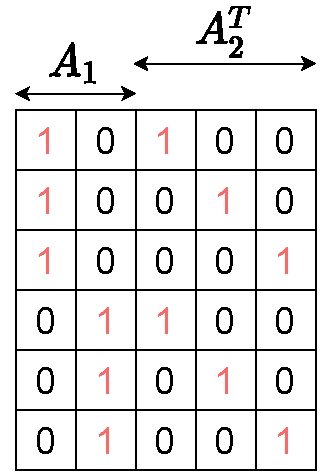
\includegraphics[height=0.25\textheight,keepaspectratio]{./Chapitre2/fig/matrix.pdf}
  \caption{An example of the matrix $A_{12}$ when $n_1=2$ and $n_2=3$.}
  \label{fig:matrix_a12}
\end{figure}

We also have that, the condition $P = P_1 \otimes P_2$ can be rewritten as
$\text{mat}(P) = \vect(P_1) \vect(P_2)^T$. By Lemma 2.1 in \citep{Joel93}, $\text{rank}_+(A) = 1$
if and only if there exist two non-negative vectors $u,v$ such that
$A = u v^T$. Thus, the factorization constraint is equivalent to
$\text{rank}_+\big( \text{mat}(P) \big) = 1$.

\subsection{MMOT-DC}

\subsection{Continuous Co-Optimal Transport} \label{annex:cont_coot}

%%%%%%%%%%%%%%%%%%%%%%%%%%%%%%%%%%%%%%%%%
\begin{proof}[Proof of \Cref{prop:exist_coot}]
  The COOT problem can be rewritten as
  \begin{equation} \label{UCOOT:1}
    \coot(\cX, \cY) = \inf_{\pi \in E_{co}} \int_{\cS} \vert c_X - c_Y \vert^p \; d\pi,
  \end{equation}
  where the set
  \begin{equation}
    E_{co} = \{ \pi \in \cP(\cS): \pi = \pi_1 \otimes \pi_2,
    \text{ where } \pi_k \in U(\mu_k^X, \mu_k^Y) \}.
  \end{equation}
  \Cref{lemma:compact_subset,lemma:coot_continuous}
  below imply that Problem \eqref{UCOOT:1} always admits a minimiser.
\end{proof}
%%%%%%%%%%%%%%%%%%%%%%%%%%%%%%%%%%%%%%%%%%%%%%%%
\begin{lemma} \label{lemma:product_polish}
  Countable product of Polish spaces is also a Polish space.
\end{lemma}
%%%%%%%%%%%%%%%%%%%%%%%%%%%%%%%%%%%%%%%%%
\begin{proof}[Proof of \Cref{lemma:product_polish}]
  First, the countable product of completely metrizable spaces is also completely metrizable
  (see for example, Proposition 1.4 in \citep{Dominique20})

  Second, we show that countable product of seperable spaces is also seperable.
  Given a sequence of seperable spaces $(X_k)_k$,
  let $\mathcal D_k$ be a countable dense subset of $X_k$. For each $k$,
  we fix a point $x_k \in X_k$. For each integer $j \geq 1$, define
  \begin{equation}
    \widetilde{\mathcal D}_j = \prod_{k=1}^j \mathcal D_k \times \prod_{k > j} \{ x_k \}
    \;\; \text{ and } \;\;
    \widetilde{\mathcal D} = \cup_{j} \widetilde{\mathcal D}_j.
  \end{equation}
  Then clearly $\widetilde{\mathcal D}_j$ is countable, for every $j \geq 1$,
  which implies $\widetilde{\mathcal D}$ is also countable.
  To show that $\widetilde{\mathcal D}$ is dense, every neighborhood $\mathcal N$ of
  $(x_1, ..., x_k, ...)$ (after reindexing) is of the form
  $\mathcal N = \prod_{k=1}^j \mathcal O_k \times \prod_{k > j} \{ x_k \}$,
  for some integer $j \geq 1$ and $\mathcal O_k \subset X_k$ is a neighborhood of $x_k$.
  As $\mathcal D_k$ is dense in $X_k$, we have $\mathcal O_k \cap \mathcal D_k \neq \emptyset$,
  thus $\mathcal N \cap \widetilde{\mathcal D} \neq \emptyset$.
  It follows that $\widetilde{\mathcal D}$ is dense in $X$.
  This concludes that the countable product of Polish spaces is also a Polish space.
\end{proof}
%%%%%%%%%%%%%%%%%%%%%%%%%%%%%%%%%%%%%%%%%%%%%%%%
\begin{lemma} \label{lemma:compact_subset}
  If $X_k$ and $Y_k$ are Polish spaces, for every $k = 1, 2$,
  then $E_{co}$ is non-empty and weakly compact in $\cP(\cS)$.
\end{lemma}
%%%%%%%%%%%%%%%%%%%%%%%%%%%%%%%%%%%%%%%%%
\begin{proof}[Proof of \Cref{lemma:compact_subset}]
  Clearly, $(\mu_1^X \otimes \mu_1^Y) \otimes (\mu_2^X \otimes \mu_2^Y) \in E_{co}$,
  so $E_{co}$ is not empty.
  We recall that $U(\mu_1^X, \mu_1^Y, \mu_2^X, \mu_2^Y)$ is the set of admissible couplings
  whose four marginals are $\mu^X_1, \mu^Y_1, \mu^X_2$ and $\mu^Y_2$. First,
  we show that $E_{co} \subset U(\mu_1^X, \mu_1^Y, \mu_2^X, \mu_2^Y)$.
  Indeed, given $\pi_k \in U(\mu_k^X, \mu_k^Y)$, for $k = 1,2$ and denote
  $\pi = \pi_1 \otimes \pi_2 \in E_{co}$. Then, for every $i, k \in \{ 1, 2 \}$ and $i \neq k$,
  we have
  \begin{equation}
      \bigg(\int_{X_{i} \times Y_{i}} d\pi_i \bigg) \int_{Y_k}  d\pi_k = d\mu_k^X.
  \end{equation}
  Other marginal distributions can be calculated in a similar manner and we conclude that
  $\pi \in U(\mu_1^X, \mu_1^Y, \mu_2^X, \mu_2^Y)$.

  As a direct generalization of Lemma 4.4 in \citep{Villani08},
  $U(\mu_1^X, \mu_1^Y, \mu_2^X, \mu_2^Y)$ is weakly compact in $\cP(\cS)$. Thus,
  to show the compactness of $E_{co}$, it is enough to show that $E_{co}$
  is a weakly closed subset of $U(\mu_1^X, \mu_1^Y, \mu_2^X, \mu_2^Y)$.
  Take a sequence $(\pi^{(n)})_n \subset E_{co}$
  such that $\pi^{(n)} \rightharpoonup \pi \in U(\mu_1^X, \mu_1^Y, \mu_2^X, \mu_2^Y)$
  (due to its compactness), we need to show that $\pi \in E_{co}$.
  As $(\pi^{(n)})_n \subset E_{co}$, there exist two sequences
  $(\pi_1^{(n)})_n \subset U(\mu_1^X, \mu_1^Y)$ and $(\pi_2^{(n)})_n \subset U(\mu_2^X, \mu_2^Y)$
  such that $\pi^{(n)} = \pi_1^{(n)} \otimes \pi_2^{(n)}$.

  For each $k = 1, 2$, due to the compactness of $U(\mu_k^X, \mu_k^Y)$ in $\cP(X_k \times Y_k)$
  (Lemma 4.4 in \citep{Villani08}), we can extract a converging subsequence
  $\pi^{(n_i^{(k)})}_k \rightharpoonup \pi_k \in U(\mu_k^X, \mu_k^Y)$, when $i \to \infty$.
  By applying Theorem 2.8 in \citep{Billingsley99} on the Polish space $\cS$
  (thanks to \Cref{lemma:product_polish}), we have
  $\pi^{(n_i^{(1)})}_1 \otimes \pi^{(n_i^{(2)})}_2 \rightharpoonup \pi_1 \otimes \pi_2 \in E_{co}$,
  when $i \to \infty$. This implies $\pi = \pi_1 \otimes \pi_2$, thus $\pi \in E_{co}$.
\end{proof}
%%%%%%%%%%%%%%%%%%%%%%%%%%%%%%%%%
%%%%%%%%%%%%%%%%%%%%%%%%%%%%%%%%%%%%%%%%%%%%%%%%
\begin{lemma} \label{lemma:coot_continuous}
    If $c_X$ and $c_Y$ are bounded measurable functions, then
    the functional $F: \pi \to \Big( \int_{\cS} \vert c_X - c_Y \vert^p \; d\pi \Big)^{1/p}$ is continuous on $E_{co}$.
\end{lemma}
%%%%%%%%%%%%%%%%%%%%%%%%%%%%%%%%%%%%%%%%%
\begin{proof}[Proof of \Cref{lemma:coot_continuous}]
  It is enough to show that $F$ is continuous on $U(\mu_1^X, \mu_1^Y, \mu_2^X, \mu_2^Y)$.
  To do this, we adapt the proof of Lemma 11 in \citep{Chowdhury19} by showing that
  there exists a sequence of continuous functions converging uniformly to $F$.

  As $\cC_b$ is dense in $L^p$ (by applying Proposition 7.9 in \citep{Folland99}
  on Polish spaces endowed with finite measures), there exist two sequences of
  bounded continuous functions $(c_X^{(n)})_n \subset L^p(X, \mu^X)$ and
  $(c_Y^{(n)})_n \subset L^p(Y, \mu^Y)$ such that
  $\vert\vert c_X - c_X^{(n)} \vert\vert_{L^p(X, \mu^X)} \leq 1/n$ and
  $\vert\vert c_Y - c_Y^{(n)} \vert\vert_{L^p(Y, \mu^Y)} \leq 1/n$.

  For each $n \in \bbN$, define $F_n: U(\mu_1^X, \mu_1^Y, \mu_2^X, \mu_2^Y) \to \bbR_{\geq 0}$
  by $F_n(\pi) = \vert\vert c_X^{(n)} - c_Y^{(n)} \vert\vert_{L^p(\cS, \pi)}$.

  The compactness of $U(\mu_1^X, \mu_1^Y, \mu_2^X, \mu_2^Y)$ implies that, for every
  $\pi \in U(\mu_1^X, \mu_1^Y, \mu_2^X, \mu_2^Y)$,
  there exists a sequence $(\pi^{(m)})_m \subset U(\mu_1^X, \mu_1^Y, \mu_2^X, \mu_2^Y)$ such that
  $\pi^{(m)} \rightharpoonup \pi$. In particular, as
  $\vert c_X^{(n)} - c_Y^{(n)} \vert^p \in \cC_b(\cS)$, we have
  \begin{equation}
    \begin{split}
      \lim_{m \to \infty} F_n(\pi^{(m)}) =
      \lim_{m \to \infty} \Big( \int_{\cS} \vert c_X^{(n)} - c_Y^{(n)} \vert^p \;
      d\pi^{(m)} \Big)^{1/p}
      = \Big( \int_{\cS} \vert c_X^{(n)} - c_Y^{(n)} \vert^p \; d\pi \Big)^{1/p} = F_n(\pi).
    \end{split}
  \end{equation}
  We deduce that $F_n$ is sequentially continuous, thus continuous
  (by Remark 5.1.1 in \citep{Ambrosio05}).
  Now, for any $\pi \in U(\mu_1^X, \mu_1^Y, \mu_2^X, \mu_2^Y)$, we have
  \begin{equation}
    \begin{split}
      \vert F_n(\pi) - F(\pi) \vert &=
      \Big\vert \vert\vert c_X^{(n)} - c_Y^{(n)} \vert\vert_{L^p(\cS, \pi)}
      - \vert\vert c_X - c_Y \vert\vert_{L^p(\cS, \pi)} \Big\vert \\
      &\leq \vert\vert c_X^{(n)} - c_Y^{(n)} - (c_X - c_Y) \vert\vert_{L^p(\cS, \pi)} \\
      &\leq \vert\vert c_X^{(n)} - c_X \vert\vert_{L^p(\cS, \pi)} +
      \vert\vert c_Y^{(n)} - c_Y \vert\vert_{L^p(\cS, \pi)} \\
      &= \vert\vert c_X^{(n)} - c_X \vert\vert_{L^p(X, \mu^X)} +
      \vert\vert c_Y^{(n)} - c_Y \vert\vert_{L^p(Y, \mu^Y)} \\
      &\leq 2/n.
    \end{split}
  \end{equation}
  The first inequality follows from a consequence of Minkowski's inequality:
  $ \Big\vert \vert\vert f \vert\vert - \vert\vert g \vert\vert \Big\vert
  \leq \vert\vert f-g \vert\vert$. The second inequality is the Minkowski's inequality.
  This implies that $F_n$ converges uniformly to $F$, thus $F$ is continuous.
\end{proof}
%%%%%%%%%%%%%%%%%%%%%%%%%%%%%%%%%%%%%%%%%%%%%%%%

Before proving the isomorphism and metric properties of COOT, let us first introduce the Monge's
formulation of COOT.
\begin{align}
  \mcoot(\cX, \cY) =
  \inf_{\substack{T_1 \in \cT(\mu^X_1, \mu^Y_1) \\ T_2 \in \cT(\mu^X_2, \mu^Y_2)}}
  \iint \Big|c_X(x_1, x_2) - c_Y \big( T_1(x_1), T_2(x_2) \big) \Big|^p
  \; d\mu^X_1(x_1) \; d\mu^X_2(x_2).
\end{align}
where recall that
$\cT(\mu^X_k, \mu^Y_k) = \{T: X_k \to Y_k \text{ such that } T_{\# \mu^X_k} = \mu^Y_k \}$,
for $k=1,2$. It is not difficult to see that, $\mcoot(\cX, \cY) = 0$ if and only if
$\cX \in \rms(\cY)$. Similar to the GW and Gromo-Monge distances, we have
%%%%%%%%%%%%%%%%%%%%%%%%%%%%%%%
\begin{corollary} \label{coro:coot_mcoot}
  Let $\cX$ and $\cY$ be two measure hypernetworks, then
  \begin{equation}
    \coot(\cX, \cY) = \inf_{\cZ \in \rms(\cX)} \mcoot(\cZ, \cY)
    = \inf_{\cZ \in \rms(\cY)} \mcoot(\cZ, \cX).
  \end{equation}
  Moreover, the infima are always attained: there exist two measure hypernetworks
  $\cZ_x \in \rms(\cX)$ and $\cZ_y \in \rms(\cY)$ such that
  $\coot(\cX, \cY) = \mcoot(\cZ_x, \cY) = \mcoot(\cZ_y, \cX)$.
\end{corollary}
The proof is adapted directly from that of Theorem 14 in \citep{Memoli21}.
For self-contained purpose, we provide the complete proof here.
%%%%%%%%%%%%%%%%%%%%%%%%%%%%%%%%%%%%%%%%%
\begin{proof}[Proof of \Cref{coro:coot_mcoot}]
  Let $(\pi_1^*, \pi_2^*)$ be a solution of the problem $\coot(\cX, \cY)$.
  For $k=1,2$, define the space $Z_k = X_k \times Y_k$
  equipped with the probability measure $\mu_k^Z = \pi_k^* \in U(\mu_k^X, \mu_k^Y)$.
  Define the projection map $P_{X_k}: Z_k \to X_k$ by $P_{X_k}(x,y) = x$ and denote
  $c_Z = (P_{X_1}, P_{X_2})^*c_X$. Clearly, the measure hypernetwork
  $\cZ := ((Z_1, \mu_1^Z), (Z_2, \mu_2^Z), c_Z)$ is a RMS of $\cX$. For
  $k=1,2$, consider the canonical projection map $P_{Y_k}: Z_k \to Y_k$ defined by $P_{Y_k}(x,y) = y$,
  then $P_{Y_k}$ is a transport map from $\mu_k^Z$ to $\mu_k^Y$. Now, as
  $(P_{X_k}, P_{Y_k})_{\#} \mu_k^Z = (P_{X_k}, P_{Y_k})_{\#} \pi_k^* = \pi_k^*$,
  for $k=1,2$, we have
  \begin{align}
    \mcoot(\cZ, \cY) &\leq \int_{Z_1 \times Z_2}
    \big\vert c_Z - (P_{Y_1}, P_{Y_2})^*c_Y \big\vert^p \; d\mu_1^Z \; d\mu_2^Z \\
    &= \int_{Z_1 \times Z_2}
    \big\vert (P_{X_1}, P_{X_2})^*c_X - (P_{Y_1}, P_{Y_2})^*c_Y \big\vert^p
    \; d\mu_1^Z \; d\mu_2^Z \\
    &= \int_{S} \vert c_X - c_Y \vert^p
    \; d(P_{X_1}, P_{Y_1})_{\#} \mu_1^Z \; d(P_{X_2}, P_{Y_2})_{\#} \mu_2^Z \\
    &= \int_{S} \vert c_X - c_Y \vert^p \; d\pi_1^* \; d\pi_2^* \\
    &= \coot(\cX, \cY),
  \end{align}
  and consequently,
  \begin{equation}
    \label{eq:coot_geq_mcoot}
    \coot(\cX, \cY) \geq \inf_{\cZ \in \rms(\cX)} \mcoot(\cZ, \cY).
  \end{equation}
  For the reverse direction, let $\cZ$ be a RMS of $\cX$. Then,
  there exist two transport maps $f_k : Z_k \to X_k$, for $k=1,2$ such that $c_Z = (f_1, f_2)^*c_X$,
  for $\mu_1^Z \otimes \mu_2^Z$-almost everywhere.
  The inequality \eqref{eq:coot_geq_mcoot} implies that we can safely exclude every
  $\cZ \in \rms(\cX)$ with $\mcoot(\cZ, \cY) = \infty$ and consider only those with
  $\mcoot(\cZ, \cY) < \infty$. In this case, there always exists a transport map
  $g_k$ from $\mu_k^Z$ to $\mu_k^Y$, for each $k=1,2$. If we define the map
  $(f_k, g_k): Z_k \to X_k \times Y_k$ by $(f_k,g_k)(z_k) = (f_k(z_k), g_k(z_k))$,
  then $(f_k,g_k)_{\# \mu_k^Z} \in U(\mu_k^X, \mu_k^Y)$, for any $k=1,2$. Now,
  \begin{align}
    \coot(\cX, \cY) &\leq \int_{S} \vert c_X - c_Y \vert^p
    \; d (f_1,g_1)_{\#} \mu_1^Z \; d (f_2,g_2)_{\#} \mu_2^Z \\
    &= \int_{Z_1 \times Z_2} \vert (f_1,f_2)^*c_X - (g_1,g_2)^*c_Y \vert^p \; d\mu_1^Z \; d\mu_2^Z \\
    &= \int_{Z_1 \times Z_2} \vert c_Z - (g_1,g_2)^*c_Y \vert^p \; d\mu_1^Z \; d\mu_2^Z.
  \end{align}
  As this is true for any $\cZ \in \rms(\cX)$ and any corresponding pair of transport maps
  $(g_1, g_2)$, we have
  \begin{equation}
    \coot(\cX, \cY) \leq \inf_{\cZ \in \rms(\cX)} \mcoot(\cZ, \cY).
  \end{equation}
  The equality then follows. Moreover, the first part of the proof also
  shows us how to construct a minimizer $\cZ_x \in \rms(\cX)$ such that
  $\coot(\cX, \cY) = \mcoot(\cZ_x, \cY)$. Similarly, we have
  \begin{equation}
    \coot(\cY, \cX) = \inf_{\cZ \in \rms(\cY)} \mcoot(\cZ, \cX).
  \end{equation}
  By the symmetry of COOT, we deduce that
  \begin{equation}
    \inf_{\cZ \in \rms(\cX)} \mcoot(\cZ, \cY) = \inf_{\cZ \in \rms(\cY)} \mcoot(\cZ, \cX),
  \end{equation}
  and there exists $\cZ_y \in \rms(\cY)$ such that $\coot(\cX, \cY) = \mcoot(\cZ_y, \cX)$.
\end{proof}
%%%%%%%%%%%%%%%%%%%%%%%%%%%%%%%%%%%%%%%%%%%%%%%%

\begin{proof}[Proof of \Cref{prop:coot_iso}]
    Suppose two measure hypernetworks $\cX$ and $\cY$ are weakly isomorphic,
    then there exists a measure hypernetwork $\cZ^*$ which is a common RMS of $\cX$ and $\cY$.
    In particular, $\mcoot(\cZ^*, \cY) = 0$. By \Cref{coro:coot_mcoot}, we deduce that
    \begin{equation}
      \coot(\cX, \cY) = \inf_{\cZ \in \rms(\cX)} \mcoot(\cZ, \cY) = 0.
    \end{equation}
    Now, suppose $\coot(\cX, \cY)=0$, then by \Cref{coro:coot_mcoot},
    there exists a mass splitting $\cZ^*$ of $\cX$ such that
    $\mcoot(\cZ^*, \cY) = 0$. But this also means $\cZ^*$ is a RMS of $\cY$.
    We conclude that $\cX$ and $\cY$ are weakly isomorphic.
\end{proof}
%%%%%%%%%%%%%%%%%%%%%%%%%%%%%%%

%%%%%%%%%%%%%%%%%%%%%%%%%%%%%%%
\begin{proof}[Proof of \Cref{prop:metric_prop}]
    For clarity, given three measure hypernetworks $\cX, \cY$ and $\cZ$,
    we denote $\cS_{xy} = \prod_{k=1}^2 X_k \times Y_k, \cS_{yz} = \prod_{k=1}^2 Y_k \times Z_k,
    \cS_{xz} = \prod_{k=1}^2 X_k \times Z_k$ and $\cS_{xyz} = \prod_{k=1}^2 X_k \times Y_k \times Z_k$.
    \begin{enumerate}
      \item The positiveness is trivial. By \Cref{prop:coot_iso},
      $\coot(\cX, \cY) = 0$ if and only if $\cX$ and $\cY$ are weakly isomorphic.

      \item To show the symmetry, for each $k = 1, 2$, we define the bijection
      $f_k: X_k \times Y_k \to Y_k \times X_k$ by $f_k(x_k,y_k) = (y_k,x_k)$.
      Then, for any $\pi_k \in U(\mu_k^X, \mu_k^Y)$, where $k=1,2$, we have
      $(f_k)_{\#} \pi_k \in U(\mu_k^Y, \mu_k^X)$ and
      \begin{equation}
        \begin{split}
          \coot(\cX, \cY) &= \inf_{\substack{\pi_k \in U(\mu^X_k, \mu^Y_k) \\
          \forall k = 1,2}} \int_{\cS_{xy}} \vert c_X - c_Y \vert^p \; d \pi_1 \; d \pi_2 \\
          &= \inf_{\substack{\pi_k \in U(\mu^X_k, \mu^Y_k) \\
          \forall k = 1,2}} \int_{\cS_{yx}} \vert c_Y - c_X \vert^p \; d (f_1)_{\#} \pi_1 \; d (f_2)_{\#} \pi_2 \\
          &= \inf_{\substack{\gamma_k \in U(\mu^Y_k, \mu^X_k) \\
          \forall k = 1,2}} \int_{\cS_{yx}} \vert c_Y - c_X \vert^p \; d \gamma_1 \; d \gamma_2 \\
          &= \coot(\cY, \cX).
        \end{split}
      \end{equation}

      \item Now, we show the triangle inequality. Let $(\pi^{(YZ)}_1, \pi^{(YZ)}_2)$ and
      $(\pi^{(XZ)}_1, \pi^{(XZ)}_2)$ be the optimal couplings which minimize
      $\coot(\cY, \cZ)$ and $\coot(\cX, \cZ)$, respectively, where
      $\pi^{(YZ)}_k$ and $\pi^{(XZ)}_k$ are in $U(\mu_k^Y, \mu_k^Z)$ and $U(\mu_k^X, \mu_k^Z)$,
      respectively, for every $k=1,2$.

      For each $k = 1,2$, by the glueing lemma (Lemma 7.6 in \citep{Villani03}), there exists a probability measure
      $\sigma_k \in \cP(X_k \times Y_k \times Z_k)$ such that
      $(P_{X_k Y_k})_{\#} \sigma_k = \pi^{(XY)}_k$ and
      $(P_{X_k Y_k})_{\#} \sigma_k = \pi^{(YZ)}_k$. Here, we define the projection maps
      \begin{itemize}
        \item[$\bullet$] $P_{X_k}: X_k \times Y_k \times Z_k \to X_k$, where
        $P_{X_k}(x,y,z) = x$.
        \item[$\bullet$] $P_{X_k Y_k}: X_k \times Y_k \times Z_k \to X_k \times Y_k$,
        where $P_{X_k Y_k}(x,y,z) = (x,y)$.
        \item[$\bullet$] $P_{X_1 Z_1 X_2 Z_2}: \cS_{xyz} \to \cS_{xz}$, where
        $P_{X_1 Z_1 X_2 Z_2}(x_1,y_1,z_1, x_2, y_2, z_2) = (x_1,z_1, x_2, z_2)$.
      \end{itemize}
      and all other projection maps are defined similarly. It follows that
      $(P_{X_k})_{\#} \sigma_k = \mu_k^X$ and $(P_{Z_k})_{\#} \sigma_k = \mu_k^Z$, thus
      $(P_{X_k Z_k})_{\#} \sigma_k \in U(\mu_k^X, \mu_k^Z)$. Furthermore, one also has
      $(P_{X_1 Z_1 X_2 Z_2})_{\#} \sigma =
      (P_{X_1 Z_1})_{\#} \sigma_1 \otimes (P_{X_2 Z_2})_{\#} \sigma_2$,
      where $\sigma = \sigma_1 \otimes \sigma_2$. Indeed, for any function $\phi \in \cC_b(\cS_{xz})$, we have
      \begin{equation}
        \begin{split}
          \int_{\cS_{xz}} \phi \; d(P_{X_1 Z_1 X_2 Z_2})_{\#} \sigma
          &= \int_{\cS_{xyz}} (\phi \circ P_{X_1 Z_1 X_2 Z_2}) \; d\sigma \\
          &= \int_{\cS_{xyz}} (P_{X_1 Z_1}, P_{X_2 Z_2})^*\phi
          \; d \sigma_1 \; d \sigma_2 \\
          &= \int_{\cS_{xz}} \phi \; d (P_{X_1 Z_1})_{\#} \sigma_1 \;
          d (P_{X_2 Z_2})_{\#} \sigma_2.
        \end{split}
      \end{equation}
      Here, with slight abuse of notation, we write $\phi(x_1,y_1, x_2,y_2) = \phi\big( (x_1,y_1), (x_2,y_2) \big)$. Now,
      \begin{equation}
        \begin{split}
          &\coot(\cX, \cZ)^{1/p} \\
          &\leq \Big( \int_{\cS_{xz}} \vert c_X - c_Z \vert^p
          \; d (P_{X_1 Z_1})_{\#} \sigma_1 \; d (P_{X_2 Z_2})_{\#} \sigma_2 \Big)^{1/p} \\
          &= \Big( \int_{\cS_{xz}} \vert c_X - c_Z \vert^p
          \; d(P_{X_1 Z_1 X_2 Z_2})_{\#} \sigma \Big)^{1/p} \\
          &= \Big( \int_{\cS_{xyz}} \big( \vert c_X - c_Z \vert^p \circ P_{X_1 Z_1 X_2 Z_2} \big)
          \; d \sigma \Big)^{1/p} \\
          &\leq \Big( \int_{\cS_{xyz}} \big( \vert c_X - c_Y \vert^p \circ P_{X_1 Y_1 X_2 Y_2} \big)
          \; d \sigma \Big)^{1/p} +
          \Big( \int_{\cS_{xyz}} \big( \vert c_Y - c_Z \vert^p \circ P_{Y_1 Z_1 Y_2 Z_2} \big)
          \; d \sigma \Big)^{1/p} \\
          &= \Big( \int_{\cS_{xy}} \vert c_X - c_Y \vert^p
          \; d (P_{X_1 Y_1 X_2 Y_2})_{\#} \sigma \Big)^{1/p}  +
          \Big( \int_{\cS_{yz}} \vert c_Y - c_Z \vert^p
          \; d (P_{Y_1 Z_1 Y_2 Z_2})_{\#} \sigma \Big)^{1/p}  \\
          &= \Big( \int_{\cS_{xy}} \vert c_X - c_Y \vert^p
          \; d (P_{X_1 Y_1})_{\#} \sigma_1 \; d (P_{X_2 Y_2})_{\#} \sigma_2 \Big)^{1/p} \\
          &+ \Big( \int_{\cS_{yz}} \vert c_Y - c_Z \vert^p
          \; d (P_{Y_1 Z_1})_{\#} \sigma_1 \; d (P_{Y_2 Z_2})_{\#} \sigma_2 \Big)^{1/p} \\
          &= \Big( \int_{\cS_{xy}} \vert c_X - c_Y \vert^p \; d \pi^{(XY)}_1 \; d \pi^{(XY)}_2 \Big)^{1/p}  +
          \Big( \int_{\cS_{yz}} \vert c_Y - c_Z \vert^p \; d \pi^{(YZ)}_1 \; d \pi^{(YZ)}_2 \Big)^{1/p} \\
          &= \coot(\cX, \cY)^{1/p} + \coot(\cY, \cZ)^{1/p}.
        \end{split}
      \end{equation}
      The first inequality is due to the sub-optimality of
      $((P_{X_1 Z_1})_{\#} \sigma_1, (P_{X_2 Z_2})_{\#} \sigma_2)$. The second one is
      the Minkowski inequality and the fact that:
      $|c_X(x_1,x_2) - c_Y(y_1,y_2)| \leq |c_X(x_1,x_2) - c_Z(z_1,z_2)| + |c_Z(z_1,z_2) - c_Y(y_1,y_2)|$,
      or more compactly
      \begin{equation}
        \vert c_X - c_Z \vert \circ P_{X_1 Z_1 X_2 Z_2} \leq
        \vert c_X - c_Y \vert \circ P_{X_1 Y_1 X_2 Y_2} +
        \vert c_Y - c_Z \vert \circ P_{Y_1 Z_1 Y_2 Z_2}.
      \end{equation}
    \end{enumerate}
\end{proof}
%%%%%%%%%%%%%%%%%%%%%%%%%%%%%%%%%

%%%%%%%%%%%%%%%%%%%%%%%%%%%%%%%
\begin{proof}
    This is an adaptation from the proof of quantitative bound between OT and regularized OT
    in \citep{Genevay19}.
    Let $\pi^* \in E_{co}$ be a solution of COOT and denote $\pi_{\Delta}$
    its block approximation at scale $\Delta > 0$.
    Clearly, $\pi_{\Delta} \in E_{co}$. The sub-optimality of $\pi_{\Delta}$ implies
    \begin{equation}
      \begin{split}
        0 &\leq \coot_{\varepsilon}(\cX, \cY) - \coot(\cX, \cY) \\
        &\leq \langle \pi_{\Delta}, \vert c_X - c_Y \vert^p \rangle
        - \langle \pi^*, \vert c_X - c_Y \vert^p \rangle +
        \varepsilon \kl(\pi_{\Delta} \vert \mu_1 \otimes \mu_2).
      \end{split}
    \end{equation}
    Now, using the fact that $\vert x - y \vert \leq \max(x,y)$, for every $x, y \geq 0$,
    and for any $i,j$,
    \begin{equation}
      \sup_{(x_1, x_2) \in Q^{\Delta}_{ij}} c_X(x_1,x_2) \leq
      L^a \sup_{(x_1, x_2) \in Q^{\Delta}_{ij}} \vert\vert x_1 - x_2 \vert\vert^a \leq (L \Delta d_x^{1/p})^a,
    \end{equation}
    we have
    \begin{equation}
      \begin{split}
        \langle \pi_{\Delta}, \vert c_X - c_Y \vert^p \rangle
        - \langle \pi^*, \vert c_X - c_Y \vert^p \rangle
        &\leq \langle \pi_{\Delta}, \vert c_X - c_Y \vert^p \rangle \\
        &\leq \sup_{i,j,k,l} \sup_{\substack{(x_1, x_2) \in Q^{\Delta}_{ij} \\ (y_1,y_2) \in Q^{\Delta}_{kl}}}
        \vert c_X(x_1,x_2) - c_Y(y_1,y_2) \vert^p \\
        &\leq \max\big( \sup_{(x_1, x_2) \in Q^{\Delta}_{ij}} c_X(x_1,x_2)^p,
        \sup_{(y_1, y_2) \in Q^{\Delta}_{kl}} c_Y(y_1,y_2)^p \big) \\
        &\leq \max\big( (\Delta Ld_x^{1/p})^{ap}, (\Delta Ld_y^{1/p})^{ap} \big) \\
        &= (\Delta Ld^{1/p})^{ap}.
      \end{split}
    \end{equation}
    The bound for the entropy term is
    \begin{equation}
      \begin{split}
        H(\pi^{\Delta}) \leq (d_x + d_y) \log(\frac{2D}{\Delta}) \leq 2 d \log(\frac{2D}{\Delta}).
      \end{split}
    \end{equation}
    Thus
    \begin{equation}
      \langle \pi_{\Delta}, \vert c_X - c_Y \vert^p \rangle -
      \langle \pi^*, \vert c_X - c_Y \vert^p \rangle + \varepsilon H(\pi^{\Delta})
      \leq (\Delta Ld^{1/p})^{ap} + 2 d \varepsilon \log(\frac{2D}{\Delta}).
    \end{equation}
    The RHS is a convex function of $\Delta$, thus admits a minimiser
    $\Delta^{ap} = \frac{2d \varepsilon}{ap (Ld^{1/p})^{ap}}$, thus
    \begin{equation}
      \langle \pi_{\Delta}, \vert c_X - c_Y \vert^p \rangle
      - \langle \pi^*, \vert c_X - c_Y \vert^p \rangle + \varepsilon H(\pi^{\Delta})
      \leq \frac{2 d \varepsilon}{ap}
      + \frac{2d \varepsilon}{ap} \log\Big( \frac{ap (2DLd^{1/p})^{ap}}{2d \varepsilon} \Big).
    \end{equation}
\end{proof}
%%%%%%%%%%%%%%%%%%%%%%%%%%%%%%%

%%%%%%%%%%%%%%%%%%%%%%%%%%%%%%
\begin{proof}
    Recall that
    \begin{equation}
      E_{co} = \{ \pi \in \cP(\cS): \pi = \pi_1 \otimes \pi_2,
      \text{ where } \pi_k \in U(\mu_k^X, \mu_k^Y) \}.
    \end{equation}
    First, observe that if $\pi \in E_{co}$ is a solution of COOT, then for any $\gamma \in E_{co}$, one has
    \begin{equation}
      \begin{split}
        0 &\leq \coot_{\varepsilon}(\cX, \cY) - \coot(\cX, \cY) \\
        &\leq \left( \int_{\cS} \vert c_X - c_Y \vert^p \; d\gamma - \int_{\cS} \vert c_X - c_Y \vert^p \; d\pi \right) +
        \varepsilon \kl(\gamma \vert \mu_1 \otimes \mu_2).
      \end{split}
    \end{equation}
    The idea is to choose $\gamma \in E_{co}$ such that, for small $\varepsilon$, the quantity inside the bracket can be arbitrarily small
    (but still positive, due to the optimality of $\pi$), and the KL divergence is always controlled, so that it does not blow up too fast.
    To do so, we extend the block approximation technique in
    \citep{Carlier17} to the multi-marginal case.
    \begin{definition}
      (Block approximation) Given an integer $K \geq 2$ and $p \geq 1$. For each $k=1,...,K$,
      let $\mu_k \in \cP(\bbR^{n_k})$, for some integer $n_k \geq 1$, be a probability measure
      with finite entropy and $p^{\text{th}}$-moment and
      absolutely continuous with respect to the Lebesgue measure.

      For each $a_k = (a_k^{(1)}, ...,a_k^{(n_k)}) \in \cZ^{n_k}$, we define the unit hypercube
      $Q_{a_k} = [a_k^{(1)}, a_k^{(1)} + 1) \times ... \times [a_k^{(n_k)}, a_k^{(n_k)} + 1) \subset \bbR^{n_k}$ and for $\Delta > 0$,
      we denote $Q^{\Delta}_{a_k} = \Delta \cdot Q_{a_k} \subset \bbR^{n_k}$ the rescaled hypercube by $\Delta$ of $Q_{a_k}$.
      For each $\pi \in \cP(\prod_k \bbR^{n_k})$, we define its block approximation at scale $\Delta$ by
      \begin{equation}
        \pi_{\Delta} := \sum_{\substack{a_k \in \cZ^{n_k} \\ k = 1, ..., K}}
        \pi \big(\prod_{k=1}^K Q^{\Delta}_{a_k}\big) \big( \otimes_{k=1}^K \mu_k^{\Delta} \big),
      \end{equation}
      where, for every Borel set $E_k \subset \bbR^{n_k}, \mu_k^{\Delta}$ is the restriction of $\mu_k$ on $Q^{\Delta}_{a_k}$ defined by
      \begin{equation}
        \mu_k^{\Delta}(E_k):=
        \begin{cases}
          \frac{\mu_k(E_k \cap Q^{\Delta}_{a_k})}{\mu_k(Q^{\Delta}_{a_k})} \; ,\text{ if } \mu_k(Q^{\Delta}_{a_k}) > 0 \\
          0 \;\;\;\;\;\;\;\;\;\;\;\;\;\;\;\;,\text{ otherwise}.
        \end{cases}
      \end{equation}
    \end{definition}
    It is not difficult to see that block approximation of a product measure is also a product measure. Indeed, it is enough to consider the case
    $K=2$. Suppose that $\pi = \pi_1 \otimes \pi_2$, then,
    \begin{equation}
      \pi_{\Delta} = \sum_{a_1, a_2}
      \pi_1(Q^{\Delta}_{a_1}) \; \pi_2(Q^{\Delta}_{a_2}) \; \mu_1^{\Delta} \otimes \mu_2^{\Delta} =
      \left( \sum_{a_1} \pi_1(Q^{\Delta}_{a_1}) \; \mu_1^{\Delta} \right) \otimes
      \left( \sum_{a_2} \pi_2(Q^{\Delta}_{a_2}) \; \mu_2^{\Delta} \right).
    \end{equation}
    %%%%%%%%%%%%%%%%%%%%%%%%%%%%%%%%%%%%%%%%%%%%%
    \begin{lemma}
        \label{lemma:block_approx}
      Recall that $U(\mu_1, ..., \mu_K)$ is the set of couplings whose marginals are $\mu_1,...,\mu_K$.
      For each $\pi \in U(\mu_1, ..., \mu_K)$, denote $\pi_{\Delta}$ its block approximation at scale $\Delta > 0$.
      \begin{enumerate}
        \item The entropy $H(\pi)$ is well defined and
        \begin{equation}
          \kl(\pi \vert \otimes_k \mu_k) = H(\pi) - \sum_{k=1}^K H(\mu_k).
        \end{equation}

        \item For every $\Delta > 0, \pi_{\Delta} \in U(\mu_1, ..., \mu_K)$.

        \item Suppose the product space $\prod_k \bbR^{n_k}$ is endowed with the metric
        \begin{equation}
          d((x_1, ..., x_K), (y_1, ..., y_K)) = \Big( \sum_{k=1}^K \vert\vert x_k - y_k \vert\vert^p \Big)^{1/p}.
        \end{equation}
        Then
        \begin{equation}
          W^p_{d^p}(\pi, \pi_{\Delta}) \leq \Big( \sum_{k=1}^K n_k \Big) \Delta^p,
        \end{equation}
        where $W_{d^p}(\pi, \pi_{\Delta})$ is the $p$-Wasserstein distance between $\pi$ and $\pi_{\Delta}$ induced by the cost $d^p$.
        Consequently, $\pi_{\Delta} \rightharpoonup \pi$ when $\Delta \to 0$.

        \item There exists constants $C > 0$ and $\alpha \in (0,1)$ such that
        \begin{equation}
          \kl(\pi_{\Delta} \vert \otimes_k \mu_k) \leq
          \sum_{k=1}^K \Big( C \big( M(\mu_k) + n_k \Delta^2 + 1 \big)^{\alpha} - n_k \log \Delta \Big).
        \end{equation}
      \end{enumerate}
    \end{lemma}
    %%%%%%%%%%%%%%%%%%%%%%%%%%%%%%%%%%%%%%%%%
    \begin{proof}
      Most proofs follow directly from \citep{Carlier17}.
      \begin{enumerate}
        \item If $\pi \ll \otimes_k \mu_k$, then as $\mu_k \ll \lambda_k$, we must have $\pi \ll \otimes_k \lambda_k$. Thus $H(\pi)$ is well
        defined. Furthermore,
        \begin{equation}
          \begin{split}
            \kl(\pi \vert \otimes_k \mu_k)
            &= \int \log \Big( \frac{\pi(x_1,...,x_K)}{\mu_1(x_1)...\mu_K(x_K)} \Big) \pi(x_1, ..., x_K) \; dx_1 ... dx_K \\
            &= \int \pi \log \pi - \sum_{k=1}^K \int \pi(x_1, ..., x_K) \log \mu_k(x_k) \; dx_1 ... dx_K \\
            &= H(\pi) - \sum_{k=1}^K \int \pi_{\# k}(x_k) \log \mu_k(x_k) \; dx_k \\
            &= H(\pi) - \sum_{k=1}^K \int \mu_k(x_k) \log \mu_k(x_k) \; dx_k \\
            &= H(\pi) - \sum_{k=1}^K H(\mu_k).
          \end{split}
        \end{equation}

        \item See Proposition 2.10 in \citep{Carlier17}
        \item See Lemma 2.11 and corollary 2.12 in \citep{Carlier17}
        \item See Proposition 2.14 in \citep{Carlier17}.
      \end{enumerate}
    \end{proof}
    %%%%%%%%%%%%%%%%%%%%%%%%%%%%%%%%%%%%%%%%%%%%%
    \begin{lemma} \label{lemma:limsupinf}
      Under Assumption 2a in the Proposition ,
      let $E$ be a non-empty subset of $\cP(\cS)$ and $(\varepsilon_n)_n$ be a positive sequence converging to zero.
      Define $\widetilde{F}: \cP(\cS) \to \bbR \cup \{ \infty \}$ and
      $\widetilde{F}_n: \cP(\cS) \to \bbR \cup \{ \infty \}$ by
      \begin{equation}
        \widetilde{F}(\pi) =
        \begin{cases}
          \int_{\cS} \vert c_X - c_Y \vert^p \; d\pi, \text{ if } \pi \in E \\
          \infty \;\;\;\;\;\;\;\;\;\;\;\;\;\;\;\;\;\;\;\;\; ,\text{ otherwise},
        \end{cases}
      \end{equation}
      and
      \begin{equation}
        \widetilde{F}_n(\pi) =
        \begin{cases}
          \int_{\cS} \vert c_X - c_Y \vert^p \; d\pi + \varepsilon_n \kl(\pi \vert \mu_1 \otimes \mu_2), \text{ if } \pi \in E \\
          \infty \;\;\;\;\;\;\;\;\;\;\;\;\;\;\;\;\;\;\;\;\;\;\;\;\;\;\;\;\;\;\;\;\;\;\;\;\;\;\;\;\;\;\;\;\;\;\;\;\;\;\;\; ,\text{ otherwise}.
        \end{cases}
      \end{equation}
      \begin{enumerate}
        \item Assume that if $\pi \in E$, then so is its block approximation. Then for every $\pi \in E$ and positive sequence $(\Delta_n)_n \to 0$, we have
        \begin{equation}
          \widetilde{F}(\pi) \geq \lim\sup_{n \to \infty} \widetilde{F}_{\Delta_n}(\pi_{\Delta_n}).
        \end{equation}

        \item Let $(\pi_n)_n \subset \cP(\cS)$ be a sequence weakly converging to $\pi \in E$. Then
        \begin{equation}
          F(\pi) \leq \lim \inf_{n \to \infty} F_{n}(\pi_n).
        \end{equation}
      \end{enumerate}
    \end{lemma}
    %%%%%%%%%%%%%%%%%%%%%%%%%%%%%%%%%%%%%%%%%
    \begin{proof}
      \text{ }
      \begin{enumerate}
        \item When $\cS$ is a finite-dimensional vector space, by \Cref{lemma:block_approx} and
        definition 6.8 in \citep{Villani08}, when $n \to \infty$,
        \begin{equation}
          \int_S \vert c_X - c_Y\vert^p \; d\pi_{\Delta_n} \to \int_S \vert c_X - c_Y\vert^p \; d\pi.
        \end{equation}
        On the other hand, following \Cref{lemma:block_approx} and the proof of the proposition 2.16 in \citep{Carlier17}, we have
        \begin{equation}
          \lim\sup_{n \to \infty} \Delta_n \kl(\pi_{\Delta_n} \vert \mu_1 \otimes \mu_2) \leq 0.
        \end{equation}
        The claim then follows.

        \item This is true because the KL divergence is nonnegative and the other terms are lower semicontinuous.
      \end{enumerate}
    \end{proof}
    %%%%%%%%%%%%%%%%%%%%%%%%%%%%%%%%%%%%%%%%%%%%%
    Now, we complete the proof of the .
    When $\varepsilon \to 0$, in case of finite-dimensional spaces, if $\pi \in E_{co}$ (or $E_{gw}$), then so is its block approximation.
    We deduce from \Cref{lemma:limsupinf} that $\widetilde{F}_{n}$ $\Gamma$-converges to
    $\widetilde{F}$, whenever $E = E_{co}$ or $E = E_{gw}$. Moreover, in both cases, the weak compactness of $E$ implies the equi-coercivity
    of $\widetilde{F}_n$. By the theorems 7.8 and 7.18 in \citep{Maso93}, we deduce that
    $\coot_{\varepsilon_n}(\cX, \cY) \to \coot(\cX, \cY)$, when $\varepsilon_n \to 0$,
    and if $(\pi_{\varepsilon_n})_{n}$ is a sequence of solution of $\coot_{\varepsilon_n}(\cX, \cY)$,
    then any cluster point of $(\pi_{\varepsilon_n})_{n}$ is a solution of $\coot(\cX, \cY)$.
  \end{proof}
%%%%%%%%%%%%%%%%%%%%%%%%%%%%%%%

%%%%%%%%%%%%%%%%%%%%%%%%%%%%%%%%%%%
\section{Proofs in Chapter 3}

For later convenience, we define the function
$\vert \xi_1 - \xi_2 \vert^p: (X_1^s \times X_2^s) \times (X_1^f \times X_2^f) \to \bbR_{\geq 0}$ by
\begin{equation}
    \vert \xi_1 - \xi_2 \vert^p \big((x_1^s, x_2^s), (x_1^f, x_2^f)\big) :=
    \vert \xi_1(x_1^s, x_1^f) - \xi_2(x_2^s, x_2^f) \vert^p,
\end{equation}
and write the objective function of generalized COOT as
\begin{equation}
    F_{\lambda}(\pi^s, \pi^f) = \iint |\xi_1 - \xi_2|^p \mathrm d\pi^s \mathrm d \pi^f
    + \sum_{k=1}^2\lambda_k D_k(\pi^s_{\#k} \otimes \pi^f_{\#k} \vert \mu^s_k \otimes \mu^f_k).
\end{equation}
The generalized COOT now reads compactly as
\begin{equation} \label{eq:ucoot_copy}
%   \ucoot_{\lambda}(\cX_1, \cX_2) :=
  \inf_{\substack{\pi^s \in \cM^+(X_1^s \times X_2^s) \\
  \pi^f \in \cM^+(X_1^f \times X_2^f) \\ m(\pi^s) = m(\pi^f)}} F_{\lambda}(\pi^s, \pi^f)
\end{equation}

%%%%%%%%%%%%%%%%%%%%%%%%%%%%%%%%%%%%%%%%%%
\subsection{Proofs related to the properties of UCOOT}
%%%%%%%%%%%%%%%%%%%%%%%%%%%%%%%%%%%%%%%

%%%%%%%%%%%%%%%%%%%%%%%%%%%%%%%%%%%%%%%%%%
\begin{claim}
  When $D_k = \iota_{=}$ and $\mu_k^s, \mu_k^f$ are probability measures, for $k=1,2$,
  then we recover COOT from generalized COOT.
\end{claim}
%%%%%%%%%%%%%%%%%%%%%%%%%%%%%%%%%%%%%%%%%%
\begin{proof}
  Under the above assumptions, the generalized COOT problem becomes
  \begin{equation}
    \begin{split}
      \inf_{\substack{\pi^s \in \cM^+(X_1^s \times X_2^s) \\
      \pi^f \in \cM^+(X_1^f \times X_2^f)}}
      &\iint |\xi_1 - \xi_2|^p \mathrm d\pi^s \mathrm d \pi^f \\
      \text{subject to } &\pi^s_{\#1} \otimes \pi^f_{\#1} = \mu_1^s \otimes \mu_1^f \text{ (C1) } \\
      & \pi^s_{\#2} \otimes \pi^f_{\#2} = \mu_2^s \otimes \mu_2^f \text{ (C2) } \\
      & m(\pi^s) = m(\pi^f) \text{ (C3) }.
    \end{split}
  \end{equation}
  As $m(\pi) = m(\pi_{\#1}) = m(\pi_{\#2})$,
  for any measure $\pi$, and $\mu_k^s, \mu_k^f$ are probability measures, for $k=1,2$,
  one has $m(\pi^s) m(\pi^f) = 1$, thus $m(\pi^s) = m(\pi^f) = 1$.
  Now, the constraint C1 implies that
  $\int_{X_1^s} \mathrm d\pi^s_{\#1} \mathrm d \pi^f_{\#1}
  = \int_{X_1^s} \mathrm d\mu_1^s \mathrm d\mu_1^f$. Thus, $\pi^f_{\#1} = \mu_1^f$.
  Similarly, we have $\pi^s_{\#k} = \mu_k^s$ and $\pi^f_{\#k} = \mu_k^f$, for any $k=1,2$.
  We conclude that $\pi^f \in U(\mu_1^f, \mu_2^f)$ and $\pi^s \in U(\mu_1^s, \mu_2^s)$,
  and we obtain the COOT problem.
\end{proof}
%%%%%%%%%%%%%%%%%%%%%%%%%%%%%%%%%%%%%%%%%%

%%%%%%%%%%%%%%%%%%%%%%%%%%%%%%%%%%%%%%%%%%
\begin{proposition}
    \label{eq:ucoot_existence_copy}
  (Existence of minimizer) Denote
  $\cS := (X_1^s \times X_2^s) \times (X_1^f \times X_2^f)$.
  Problem \eqref{eq:ucoot_copy} admits a minimizer if at least one of
  the following conditions hold:
  \begin{enumerate}
    \item The entropy functions $\phi_1$ and $\phi_2$ are superlinear, \textit{i.e}.
    $(\phi_1)'_{\infty} = (\phi_2)'_{\infty} = \infty$.
    \item The function $\vert c_X - c_Y \vert^p$ has compact sublevels in $\cS$ and
    $\inf_{\cS} \vert \xi_1 - \xi_2 \vert^p + \lambda_1 (\phi_1)'_{\infty} + \lambda_2 (\phi_2)'_{\infty} > 0$.
  \end{enumerate}
\end{proposition}
%%%%%%%%%%%%%%%%%%%%%%%%%%%%%%%%%%%%%%%%%%

%%%%%%%%%%%%%%%%%%%%%%%%%%%%%%%%%%%%%%%%%%
\begin{proof}
  We adapt the proof of Theorem 3.3 in \citep{Liero18} and of Proposition 3 in \citep{Sejourne20}.
  For convenience, we write $\mu_1 = \mu_1^s \otimes \mu_1^f$ and
  $\mu_2 = \mu_2^s \otimes \mu_2^f$. For each pair $(\pi^s, \pi^f)$, denote
  $\pi = \pi^s \otimes \pi^f$.
  It can be shown that
  $\pi_{\# k} := (P_{X_k^s \times X_k^f})_{\#} \pi
  = (P_{X_k^s})_{\#} \pi^s \otimes (P_{X_k^f})_{\#} \pi^f =
  \pi^s_{\# k} \otimes \pi^f_{\# k}$, for $k=1,2$. Indeed, for any function
  $\phi \in \mathcal C_b(X_k^s \times X_k^f)$, we have
    \begin{equation}
      \begin{split}
        \int_{X_k^s \times X_k^f} \phi \;
        \mathrm d (P_{X_k^s X_k^f})_{\#} \pi
        &= \int_{\cS} (\phi \circ P_{X_k^s X_k^f}) \; \mathrm d\pi \\
        &= \int_{\cS} \phi(x_k^s, x_k^f)
        \; \mathrm d \pi^s(x_1^s, x_2^s) \; \mathrm d \pi^f(x_1^f, x_2^f) \\
        &= \int_{X_k^s \times X_k^f} \phi \; \mathrm d \pi^s_{\# k} \;
        \mathrm d \pi^f_{\# k}.
      \end{split}
    \end{equation}
  Thus, Problem \eqref{eq:ucoot_copy} can be rewritten as
  \begin{equation}
    \ucoot_{\lambda}(\cX_1, \cX_2) =
    \inf_{\pi \in E_{uco}} \int_{\cS} \vert \xi_1 - \xi_2 \vert^p
    \mathrm d\pi + \sum_{k=1,2} \lambda_k D_{\phi_k}(\pi_{\# k} \vert \mu_k),
  \end{equation}
  where
  \begin{equation}
    E_{uco} = \{ \pi \in \cM^+(\cS) \vert \pi = \pi^s \otimes \pi^f,
    \pi^s \in \cM^+(X_1^s \times X_2^s),
    \pi^f \in \cM^+(X_1^f \times X_2^f) \}.
  \end{equation}
  Define
  \begin{equation}
    L(\pi):= \int_{\cS} \vert \xi_1 - \xi_2 \vert^p \mathrm d \pi +
    \sum_{k=1,2} \lambda_k D_{\phi_k}(\pi_{\# k} \vert \mu_k).
  \end{equation}
  By Jensen's inequality, we have
  \begin{equation}
    \begin{split}
      L(\pi) &\geq m(\pi) \inf_{\cS} \vert \xi_1 - \xi_2 \vert^p +
      \sum_{k=1,2} \lambda_k m(\mu_k) \phi_k \Big( \frac{m(\pi_{\# k})}{m(\mu_k)} \Big) \\
      &= m(\pi) \bigg[ \inf_{\cS} \vert \xi_1 - \xi_2 \vert^p +
      \sum_{k=1,2} \lambda_k \frac{m(\mu_k)}{m(\pi)} \phi_k
      \Big( \frac{m(\pi)}{m(\mu_k)} \Big) \bigg],
    \end{split}
  \end{equation}
  where, in the last equality, we use the relation $m(\pi) = m(\pi_{\# k})$, for $k=1,2$.
  It follows from the assumption that $L$ is coercive. So, $L(\pi) \to \infty$
  when $m(\pi) \to \infty$.

  Clearly $\inf_{E_{uco}} L < \infty$ because
  $L\big( (\mu_1^s \otimes \mu_2^s) \otimes (\mu_1^f \otimes \mu_2^f) \big) < \infty$.
  Let $(\pi_n)_n \subset {E_{uco}}$ be a minimizing sequence, meaning that
  $L(\pi_n) \to \inf_{E_{uco}} L$.
  Such sequence is necessarily bounded (otherwise, there exists a subsequence $(\pi_{n_k})_{n_k}$
  with $m(\pi_{n_k}) \to \infty$ and the coercivity of $L$ implies $L(\pi_{n_k}) \to \infty$,
  which is absurd). Suppose $m(\pi_{n}) \leq M$, for some $M > 0$. By Tychonoff's theorem,
  as $X_k^s$ and $X_k^f$ are compact spaces,
  so is the product space $\cS$. Thus, by Banach-Alaoglu theorem,
  the ball $B_M = \{ \pi \in \cM^+(\cS): m(\pi) \leq M \}$
  is weakly compact in $\cM^+(\cS)$.

  Consider the set $\overline{E}_{uco} = E_{uco} \cap B_M$, then clearly
  $(\pi_n)_n \subset \overline{E}_{uco}$. We will show that
  there exists a converging subsequence of $(\pi_n)_n$, whose limit is in $\overline{E}_{uco}$,
  thus $\overline{E}_{uco}$ is weakly compact. Indeed, by definition of $E_{uco}$,
  there exist two sequences $(\pi_n^s)_n$ and $(\pi_n^f)_n$ such that
  $\pi_n = \pi_n^s \otimes \pi_n^f$.
  We can assume furthermore that $m(\pi_n^s) = m(\pi_n^f) = \sqrt{m(\pi_n)} \leq \sqrt M$.
  As $m(\pi_n^s)$ and $m(\pi_n^f)$ are bounded, by reapplying Banach-Alaoglu theorem,
  one can extract two converging subsequences (after reindexing)
  $\pi_n^s \rightharpoonup \pi^s \in \cM^+(X_1^s \times X_2^s)$ and
  $\pi_n^f \rightharpoonup \pi^f \in \cM^+(X_1^f \times X_2^f)$,
  with $m(\pi^s) = m(\pi^f) \leq \sqrt{M}$.
  An immediate extension of Theorem 2.8 in \citep{Billingsley99} to the convergence of
  the products of bounded positive measures implies
  $\pi_n^s \otimes \pi_n^f \rightharpoonup \pi^s \otimes \pi^f \in \overline{E}_{uco}$.

  Now, the lower semicontinuity of $L$ implies that $\inf_{E_{uco}} L \geq L(\pi^s \otimes \pi^f)$,
  thus $L(\pi^s \otimes \pi^f) = \inf_{E_{uco}} L$ and $(\pi^s, \pi^f)$
  is a solution of Problem \eqref{eq:ucoot_copy}.
\end{proof}
%%%%%%%%%%%%%%%%%%%%%%%%%%%%%%%%%%%%%%%%%%%%%

%%%%%%%%%%%%%%%%%%%%%%%%%%%%%%%%%%%%%%%%%%%
\begin{claim}
  Suppose that $\cX_1$ and $\cX_2$ are two finite sample-feature spaces such that
  $(X^s_1, X^s_2)$ and $(X^f_1, X^f_2)$
  have the same cardinality and are equipped with the uniform measures
  $\mu_1^s = \mu_2^s$, $\mu_1^f = \mu_2^f$. Then $\ucoot_{\lambda}(\cX_1, \cX_2) = 0$
  if and only if there exist perfect alignments between rows (samples) and between
  columns (features) of the interaction matrices $\xi_1$ and $\xi_2$.
\end{claim}
%%%%%%%%%%%%%%%%%%%%%%%%%%%%%%%%%%%%%%%%%%%%%
\begin{proof}
  Without loss of generality, we can assume that $\mu_k^s$ and $\mu_k^f$ are
  discrete uniform probability distributions, for $k=1,2$. By Proposition 1 in \citep{Redko20},
  under the assumptions on $\cX_1$ and $\cX_2$, we have
  $\coot(\cX_1, \cX_2) = 0$ if and only if there exist perfect alignments
  between rows (samples) and between columns (features) of the interaction matrices $\xi_1$ and
  $\xi_2$. So, it is enough to prove that $\ucoot_{\lambda}(\cX_1, \cX_2) = 0$
  if and only if $\coot(\cX_1, \cX_2) = 0$.

  Let $(\pi^s, \pi^f)$ be a pair of equal-mass couplings such that
  $\ucoot_{\lambda}(\cX_1, \cX_2) = 0$. It follows that
  $\pi^s_{\#k} \otimes \pi^f_{\#k} = \mu_k^s \otimes \mu_k^f$, for $k=1,2$. Consequently,
  $m(\pi^s) m(\pi^f) = m(\mu_1^s) m(\mu_1^f) = 1$, so $m(\pi^s) = m(\pi^f) = 1$. Now, we have
  $\int_{X_k^s} \mathrm d \pi^s_{\#k} \; \mathrm d \pi^f_{\#k}
  = \int_{X_k^s} \mathrm d\mu_k^s \; \mathrm d\mu_k^f$, or equivalently,
  $\pi^f_{\#k} = \mu_k^f$. Similarly, $\pi^s_{\#k} = \mu_k^s$, meaning that
  $\pi^s \in U(\mu_1^s, \mu_2^s)$ and $\pi^f \in U(\mu_1^f, \mu_2^f)$. Thus,
  $\coot(\cX_1, \cX_2) = \ucoot_{\lambda}(\cX_1, \cX_2) = 0$.

  For the other direction, suppose that $\coot(\cX_1, \cX_2) = 0$.
  Let $(\pi^s, \pi^f)$ be a pair of couplings such that $\coot(\cX_1, \cX_2) = 0$.
  As $\pi^s \in U(\mu_1^s, \mu_2^s)$ and $\pi^f \in U(\mu_1^f, \mu_2^f)$, one has
  $\coot(\cX_1, \cX_2) = F_{\lambda}(\pi^s, \pi^f) \geq
  \ucoot_{\lambda}(\cX_1, \cX_2) \geq 0$,
  for every $\lambda_1, \lambda_2 > 0$. So, $\ucoot_{\lambda}(\cX_1, \cX_2) = 0$.
\end{proof}
%%%%%%%%%%%%%%%%%%%%%%%%%%%%%%%%%%%

%%%%%%%%%%%%%%%%%%%%%%%%%%%%%%%%%%%ù
\subsection{Robustness of UCOOT and sensitivity of COOT}

First, we recall our assumptions.
%%%%%%%%%%%%%%%%%%%%%%%%%%%%%%%%%%%%%%%%%
\begin{assumption}
\label{assump:robust_copy}
Consider two sample-feature spaces
$\bbX_k = ((X^s_k, \mu^s_k), (X^f_k, \mu^f_k), \xi_k)$, for $k=1,2$.
Let $\varepsilon^s$ (resp. $\varepsilon^f$) be a probability measure with compact support $O^s$
(resp. $O^f$). For $a \in \{s, f\}$, define the noisy distribution
$\widetilde{\mu}^a = \alpha_a \mu^a + (1-\alpha_a) \varepsilon^a$, where $\alpha_a \in [0,1]$.
We assume that $\xi_1$ is defined on
$(X^s_1 \cup O^s) \times (X^f_1 \cup O^f)$ and that $\xi_1, \xi_2$
are continuous on their supports. We denote the contaminated sample-feature space by
$\widetilde{\cX_1} = ((X^s_1 \cup O^s, \widetilde{\mu}^s_1),
(\cX^f_1 \cup O^f, \widetilde{\mu}^f_1), \xi_1)$. Finally,
we define some useful minimal and maximal costs:
  \[
  \begin{cases}
  \Delta_{0} =& \min_{
  \substack{
       x_1^s \in O^s, x_1^f \in O^f  \\
       x_2^s \in \cX_2^s, x_2^f \in \cX_2^f
  }}\quad |\xi_1(x_1^s, x_1^f) - \xi_2(x_2^s, x_2^f)|^p \\
  \Delta_{\infty} =& \max_{
  \substack{
  x_1^s \in \cX_1^s \cup O^s, x_1^f \in \cX_1^f \cup O^f \\
  x_2^s \in \cX_2^s, x_2^f \in \cX_2^f
  }} \quad|\xi_1(x_1^s, x_1^f) - \xi_2(x_2^s, x_2^f)|^p \enspace.
  \end{cases}
\]
\end{assumption}
For convenience, we write $C = \vert \xi_1 - \xi_2 \vert^p$ and
$\widetilde{\cS} := (X^s_1 \cup O^s) \times X_2^s \times (X^f_1 \cup O^f) \times X_2^f$.
%%%%%%%%%%%%%%%%%%%%%%%%%%%%%%%%
\begin{proposition}[COOT is sensitive to outliers]
Consider $\widetilde{\cX_1}, \cX_2$ as defined in \Cref{assump:robust_copy}.
Then:
 \label{prop:coot-not-robust_copy}
\begin{equation}
    \coot(\widetilde{\cX_1}, \cX_2) \geq (1 - \alpha_s)(1-\alpha_f) \Delta_0.
\end{equation}
%%%%%%%%%%%%%%%%%%%%%%%%%%%%%%%%%
\end{proposition}
\begin{proof}
Consider a pair of feasible alignments $(\pi^s, \pi^f)$. Since $C$ is non-negative, taking the COOT integral over a smaller set leads to the lower bound:
% \coot(\cX_1, \widetilde{\cX_2}) &= \min_{\substack{\pi^s \in \cU(\mu_1^s, \widetilde{\mu_2^s}) \\ \pi^f \in \cU(\mu_1^f, \widetilde{\mu_2^f})}}
\begin{equation}
    \begin{split}
        \int_{\widetilde{\cS}} C \mathrm d\pi^s\mathrm d\pi^f
        &\geq \int_{O^s \times \cX_2^s \times O^f \times \cX_2^f} C \mathrm d\pi^s\mathrm d\pi^f \\
          &\geq  \Delta_0 \int_{O^s \times \cX_2^s \times O^f \times \cX_2^f}  \mathrm d\pi^s\mathrm d\pi^f \\
          &= \Delta_0 \int_{O^s\times O^f}  \mathrm d\pi^s_{\#1} \mathrm d\pi^f_{\#1} \\
          &\geq (1 - \alpha_s)(1 -\alpha_f)\Delta_0,
    \end{split}
\end{equation}
where the last inequality follows from the marginal constraints.
\end{proof}

%%%%%%%%%%%%%%%%%%%%%%%%%%%%%%%%%
\begin{theorem}[UCOOT is robust to outliers]
  \label{thm:ucoot_robust_copy}
  Consider two sample-feature spaces $\widetilde{\cX_1}, \cX_2$ as defined in
  \Cref{assump:robust_copy}. Let
  $\delta = 2(\lambda_1 + \lambda_2)(1 - \alpha_s\alpha_f)$ and
  $K = M + \frac{1}{M}\ucoot(\cX_1, \cX_2) +\delta$, where
  $M= m(\pi^s) = m(\pi^f)$ is the transported mass between clean data. Then:
     \begin{equation} %\label{eq:ucoot-robust}
      \begin{split}
        \ucoot(\widetilde{\cX_1}, \cX_2)
        \leq \alpha_s \alpha_f \ucoot(\cX_1, \cX_2) +
        \delta M \left[ 1 - \exp \left( {- \frac{\Delta_{\infty}(1+M) + K}{\delta M}} \right) \right].
      \end{split}\vspace{-10mm}
    \end{equation}
  \end{theorem}
  %%%%%%%%%%%%%%%%%%%%%%%%%%%%%%%%%%%%%%%%%%%%
  To get the exponential bound of this theorem, we use the following lemma.
  \begin{lemma}
  \label{slem:bound}
  Let $\varphi: t \in (0, 1] \mapsto t\log(t) - t + 1$ and
  $f_{a, b}: t \in (0, 1] \mapsto t \to at + b \varphi(t)$ for some $a, b > 0$.
  Then:
  \begin{equation}
      \min_{t \in (0, 1]} f_{a, b}(t) = b(1 - e^{-a/b}) = f_{a, b}(e^{-\frac{a}{b}}).
  \end{equation}
  \end{lemma}
  \begin{proof}
    Since $f_{a,b}$ is convex, cancelling the gradient is sufficient for optimality.
    The solution follows immediately.
  \end{proof}
  \begin{proof}
    The proof uses the same core idea of \citep{Fatras21} but is slightly more technical
    for two reasons: (1) we consider arbitrary outlier distributions instead of simple Diracs;
    (2) we consider sample-feature outliers which requires more technical derivations.

    The idea of proof is as follows. First, we construct sample and feature couplings
    from the solution of "clean" UCOOT and the reference measures. Then, they are used to
    upper bound the "noisy" UCOOT. By manipulating this bound, the "clean" UCOOT term will appear.
    A variable $t \in (0,1)$ is also introduced in the fabricated couplings.
    The upper bound becomes a function of $t$ and can be optimized to obtain the final bound.

    Now, we prove Theorem 2.

    \paragraph{Fabricating sample and feature couplings.}
    Given the equal-mass solution $(\pi^s, \pi^f)$ of the UCOOT problem,
    with $m(\pi^s) = m(\pi^f) = M$, consider, for $t \in (0,1)$, a pair of
    sub-optimal transport plans:
    \begin{align}
      &\widetilde{\pi}^s = \alpha_s \pi^s + t (1-\alpha_s) \varepsilon_s \otimes \mu^s_2\\
      &\widetilde{\pi}^f = \alpha_f \pi^f + t (1-\alpha_f) \varepsilon_f \otimes \mu^f_2.
    \end{align}
    Then, for $a\in \{s, f\}$, it holds:
    \begin{itemize}
      \item $\widetilde{\pi}^a_{\#1} = \alpha_k \pi^a_{\#1} + t (1 - \alpha_a) \varepsilon_a$,
      \item $\widetilde{\pi}^a_{\#2} = \alpha_k \pi^a_{\#2} + t (1 - \alpha_a) \mu^a_2$,
      \item $m(\widetilde{\mu}^a_1) = 1$ and $m(\widetilde{\pi}^a) = \alpha_a M + (1-\alpha_a) t$.
    \end{itemize}
    \paragraph{Establishing and manipulating the upper bound.}
    Denote $q = (1 - \alpha_s)(1 - \alpha_f), s = \alpha_s (1-\alpha_f) + \alpha_f (1 - \alpha_s)$
    and recall that on $\widetilde{\cS}$, the cost $C$ is upper bounded by
    $\Delta_{\infty} = \max_{\widetilde{\cS}}|\xi_1 - \xi_2|^p$.
    First we upper bound the transportation cost:
    \begin{equation}
      \label{seq:cost-split}
      \begin{split}
        &\int_{\widetilde{\cS}} C \; \mathrm d\widetilde{\pi}^s \; \mathrm d\widetilde{\pi}^f \\
        &= \alpha_s\alpha_f\int_{\widetilde{\cS}} C \; \mathrm d\pi^s \; d\pi^f +
        t \sum_{k \neq i} (1-\alpha_i) \alpha_k \int_{\widetilde{\cS}} C \;
        \mathrm d \varepsilon_i \; \mathrm d\mu^i_2  \; \mathrm d\pi^k +
        q t^2 \int_{\widetilde{\cS}} C \; \mathrm d \varepsilon_s \; \mathrm d\mu_2^s \;
        \mathrm d\varepsilon_f \; \mathrm d\mu^f_2 \\
        &\leq \alpha_s\alpha_f \int_{\cS} C \; \mathrm d\pi^s \;\mathrm d\pi^f +
        \Delta_{\infty}(Ms + q)t\enspace,
      \end{split}
    \end{equation}
   since $t^2 \leq t$.

  Second, we turn to the KL marginal discrepancies. We would like to extract the KL terms
  involving only the clean transport plans from the contaminated ones.
  We first detail both joint KL divergences for the source measure indexed by 1.
  The same holds for the target measure:
    \begin{equation}
    \label{seq:kl-split}
    \begin{split}
      &\kl(\widetilde{\pi}^s_{\#1} \otimes \widetilde{\pi}^f_{\#1} \vert \widetilde{\mu}^s_1 \otimes \widetilde{\mu}^f_1) =
      \sum_{k \neq i} m(\widetilde{\pi}^i) \kl(\widetilde{\pi}^k_{\#1} \vert \widetilde{\mu}^k_1) +
      \prod_{k} \big( m(\widetilde{\pi}^k) - 1 \big)\\
      &
      \kl(\pi^s_{\#1} \otimes \pi^f_{\#1} \vert \mu^s_1 \otimes \mu^f_1) =
    M \sum_k \kl(\pi^k_{\#1} \vert \mu^k_1) + (M-1)^2.
      \end{split}
    \end{equation}
    Now we upper bound each smaller KL term using the joint convexity of the KL divergence:
    \begin{equation}
      \begin{split}
        \kl(\widetilde{\pi}^k_{\#1} \vert \widetilde{\mu}^k_1) &\leq
        \alpha_k \kl(\pi^k_{\#1} \vert \mu^k_1) + (1 - \alpha_k) \kl(t \varepsilon_k \vert \varepsilon_k) \\
        &= \alpha_k \kl(\pi^k_{\#1} \vert \mu^k_1) + (1 - \alpha_k) \varphi(t),
      \end{split}
    \end{equation}
    where $\varphi(t) = t \log t - t + 1$, for $t > 0$. Thus, for $k\neq i$:
    \begin{equation}
      \begin{split}
        &m(\widetilde{\pi}^i) \kl(\widetilde{\pi}^k_{\#1} \vert \widetilde{\mu}^k_1)
        \leq m(\widetilde{\pi}^i) \alpha_k \kl(\pi^k_{\#1} \vert \mu^k_1)
        + m(\widetilde{\pi}^i) (1 - \alpha_k) \varphi(t) \\
        &= \alpha_i\alpha_k M \kl(\pi^k_{\#1} \vert \mu^k_1)
        + t (1-\alpha_i) \alpha_k \kl(\pi^k_{\#1} \vert \mu^k_1)
        + \alpha_i(1-\alpha_k) M \varphi(t) + t q\varphi(t).
      \end{split}
    \end{equation}
    Summing over $f$ and $s$, we obtain:
    \begin{equation}
      \begin{split}
        &\sum_{k \neq i} m(\widetilde{\pi}^i) \kl(\widetilde{\pi}^k_{\#1} \vert \widetilde{\mu}^k_1) \\
        &\leq \alpha_s\alpha_f M \sum_k \kl(\pi^k_{\#1} \vert \mu^k_1) +
        t \sum_{k \neq i} (1-\alpha_i) \alpha_k \kl(\pi^k_{\#1} \vert \mu^k_1)
        + M s \varphi(t)+ 2q t \varphi(t) \\
        &\leq (\alpha_s\alpha_f + \frac{t s}{M})\left(\kl(\pi^s_{\#1} \otimes \pi^f_{\#1}
        \vert \mu^s_1 \otimes \mu^f_1) - (1-M)^2\right) + M s \varphi(t)+ 2q t \varphi(t).
        \end{split}
    \end{equation}
     where, in the last bound, we used the second equation of \eqref{seq:kl-split}
     and the fact that $\alpha_s(1-\alpha_f) \leq s$ and  $\alpha_f(1-\alpha_s) \leq s$.
     The product of masses of \eqref{seq:kl-split} can be written:
    \begin{equation}
      \begin{split}
        \prod_{k} \big( m(\widetilde{\pi}^k) - 1 \big) &= \prod_k \big( \alpha_k(M-1)
        + (1-\alpha_k)(t-1) \big) \\
        &= \alpha_s\alpha_f(1-M)^2 + s(1-M)(1-t) + q(1-t)^2.
      \end{split}
    \end{equation}
    Thus, combining these upper bounds for the source measure:
    \begin{equation}
      \begin{split}
        \kl(\widetilde{\pi}^s_{\#1} \otimes \widetilde{\pi}^f_{\#1} \vert \widetilde{\mu}^s_1 \otimes \widetilde{\mu}^f_1)
        &\leq \alpha_s\alpha_f \kl(\pi^s_{\#1} \otimes \pi^f_{\#1} \vert \mu^s_1 \otimes \mu^f_1) \\
        &+ \frac{ts}{M}\left(\kl(\pi^s_{\#1} \otimes \pi^f_{\#1} \vert \mu^s_1 \otimes \mu^f_1) - (1-M)^2\right) \\
        &+ \big[  sM \varphi(t)+ 2q t \varphi(t) + s(1-M)(1-t) + q(1-t)^2 \big],
      \end{split}
    \end{equation}
    and similarly, for the target measure:
    \begin{equation}
      \begin{split}
        \kl(\widetilde{\pi}^s_{\#2} \otimes \widetilde{\pi}^f_{\#2} \vert \mu^s_2 \otimes \mu^f_2)
        &\leq \alpha_s\alpha_f \kl(\pi^s_{\#2} \otimes \pi^f_{\#2} \vert \mu^s_2 \otimes \mu^f_2) \\
        &+ \frac{ts}{M}\left(\kl(\pi^s_{\#2} \otimes \pi^f_{\#2} \vert \mu^s_2 \otimes \mu^f_2)
        - (1-M)^2\right) \\
       &+ \big[ sM \varphi(t)+ 2q t \varphi(t) + s(1-M)(1-t) + q(1-t)^2 \big].
      \end{split}
    \end{equation}
    Then, for every $0 < t \leq 1$, by summing all bounds:
    \begin{equation}
      \begin{split}
        \ucoot(\widetilde{\cX_1}, \cX_2) &\leq \alpha_s\alpha_f \ucoot(\cX_1, \cX_2) +
        \Delta_{\infty}(Ms + q)t \\
        &+ \frac{ts}{M}(\ucoot(\cX_1, \cX_2) - (\lambda_1 + \lambda_2)(1-M)^2) \\
        &+ (\lambda_1 + \lambda_2) \big[ s M \varphi(t) + 2q t \varphi(t)
        + s(1-M)(1-t) + q(1-t)^2 \big].
      \end{split}
    \end{equation}
    \paragraph{Minimizing the upper bound with respect to $t$.}
    To obtain the exponential bound, we would like have an upper bound of the form
    $at + b\varphi(t)$, so that \Cref{slem:bound} applies.
    Knowing that $1 \leq 2(t + \varphi(t))$ for any $t \in [0, 1]$:
    Let's first isolate the quantity that is not of this form:
    We have:
    \begin{equation}
      \begin{split}
        2q t \varphi(t) + s(1 - M) + q(t-1)^2 &= 2qt^2\log(t) - 2qt^2 + 2qt + s(1-M) + qt^2 -2qt + q \\
        &=  2qt^2\log(t) - qt^2 + s(1-M) + q \\
        &= q\varphi(t^2) + s(1-M) \leq q + s(1-M) \\
        &\leq 2(q + s(1-M)) (t + \varphi(t)) \\
        &= 2(1 -\alpha_s\alpha_f - sM) (t + \varphi(t)).
      \end{split}
    \end{equation}
    The new full bound is given by:
    \begin{equation}
        \ucoot(\widetilde{\cX_1}, \cX_2) \leq \alpha_s\alpha_t \ucoot(\cX_1, \cX_2) + A' t + B'\varphi(t),
    \end{equation}
    where
    \begin{equation}
        \begin{split}
            A' &= \Delta_{\infty}(Ms + q) + s(M-1) + \frac{s}{M}\ucoot(\cX_1, \cX_2) - \frac{s}{M}(\lambda_1 + \lambda_2)(1-M)^2 \\
            &+ 2(\lambda_1 + \lambda_2) (1-\alpha_s\alpha_f - sM) \\
            & \leq \Delta_{\infty}(M + 1) + M + \frac{1}{M}\ucoot(\cX_1, \cX_2) + 2(\lambda_1 + \lambda_2) (1-\alpha_s\alpha_f) = A \\
            B' &= 2sM(\lambda_1 + \lambda_2) (1-\alpha_s\alpha_f) \leq 2M(\lambda_1 + \lambda_2) (1-\alpha_s\alpha_f) = B.
        \end{split}
    \end{equation}
    In both inequalities, we use the fact that $s \leq 1 - \alpha_s \alpha_f \leq 1$.
    Using \Cref{slem:bound}, we obtain
    \begin{equation}
        \ucoot(\widetilde{\cX_1}, \cX_2)
        \leq \alpha_s\alpha_f \ucoot(\cX_1, \cX_2) + B \left[ 1 - \exp{ \left(- \frac{A}{B} \right) }\right].
    \end{equation}
    The upper bound of \Cref{thm:ucoot_robust_copy} then follows.
  \end{proof}
%%%%%%%%%%%%%%%%%%%%%%%%%%%%%%%%%%%

%%%%%%%%%%%%%%%%%%%%%%%%%%%%%%%%%%%
\subsection{Numerical aspects}
%%%%%%%%%%%%%%%%%%%
\begin{proof}
  Denote $\pi_{\varepsilon} = \pi_{\varepsilon}^s \otimes \pi_{\varepsilon}^f$.
  \begin{enumerate}
    \item When $\varepsilon \to \infty$: the sub-optimality of
    $\left( \sqrt{\frac{m(\mu^f)}{m(\mu^s)}} \mu^s, \sqrt{\frac{m(\mu^s)}{m(\mu^f)}} \mu^f \right)$
    implies
    \begin{equation}
      \begin{split}
        \varepsilon \kl(\pi_{\varepsilon} \vert \mu^s \otimes \mu^f)
        &\leq F_{\lambda}(\pi_{\varepsilon}^s, \pi_{\varepsilon}^f) +
        \varepsilon \kl(\pi_{\varepsilon} \vert \mu^s \otimes \mu^f) \\
        &\leq F_{\lambda} \left( \sqrt{\frac{m(\mu^f)}{m(\mu^s)}} \mu^s, \sqrt{\frac{m(\mu^s)}{m(\mu^f)}} \mu^f \right) +
        \varepsilon \kl( \mu^s \otimes \mu^f \vert \mu^s \otimes \mu^f) \\
        &= \iint \vert \xi_1 - \xi_2 \vert^p \mathrm d\mu^s \mathrm d\mu^f.
      \end{split}
    \end{equation}
    Thus,
    \begin{equation}
      0 \leq \kl(\pi_{\varepsilon} \vert \mu^s \otimes \mu^f)
      \leq \frac{1}{\varepsilon} \iint \vert \xi_1 - \xi_2 \vert^p
      \mathrm d\mu^s \mathrm d\mu^f \to 0,
    \end{equation}
    whenever $\varepsilon \to \infty$. We deduce that
    $\kl(\pi_{\varepsilon} \vert \mu^s \otimes \mu^f)$,
    thus $\pi_{\varepsilon} \rightharpoonup \mu^s \otimes \mu^f$. The conclusion then follows.

    \item Let $(\pi_*^s, \pi_*^f)$ be a solution of
    $\ucoot_{\lambda}(\cX_1, \cX_2)$.
    The optimality of $(\pi_{\varepsilon}^s, \pi_{\varepsilon}^f)$ implies
    \begin{equation}
      \begin{split}
        \ucoot_{\lambda}(\cX_1, \cX_2)
      &\leq \ucoot_{\lambda}(\cX_1, \cX_2) +
      \varepsilon \kl(\pi_*^s \otimes \pi_*^f \vert \mu^s \otimes \mu^f).
      \end{split}
    \end{equation}
    Thus, when $\varepsilon \to 0$, one has
    $\ucoot_{\lambda, \varepsilon}(\cX_1, \cX_2) \to
    \ucoot_{\lambda}(\cX_1, \cX_2)$. Now, for every $\varepsilon > 0$,
    \begin{equation}
      \begin{split}
        \langle C, \mu^s \otimes \mu^f \rangle &=
        F_{\lambda} \left( \sqrt{\frac{m(\mu^f)}{m(\mu^s)}} \mu^s, \sqrt{\frac{m(\mu^s)}{m(\mu^f)}} \mu^f \right) +
        \varepsilon \kl( \mu^s \otimes \mu^f \vert \mu^s \otimes \mu^f ) \\
        &\geq F_{\lambda}(\pi_{\varepsilon}^s, \pi_{\varepsilon}^f) +
        \varepsilon \kl(\pi_{\varepsilon}^s \otimes \pi_{\varepsilon}^f \vert \mu^s \otimes \mu^f) \\
        &\geq F_{\lambda}(\pi_{\varepsilon}^s, \pi_{\varepsilon}^f).
      \end{split}
    \end{equation}
    On the other hand, following the same proof in \Cref{eq:ucoot_existence_copy},
    we can show that if
    $m(\pi_{\varepsilon}) \to \infty$, then
    $F_{\lambda}(\pi_{\varepsilon}^s, \pi_{\varepsilon}^f) \to \infty$, which
    contradicts the above inequality. So, there exists $M > 0$ such that
    $m(\pi_{\varepsilon}) \leq M$, for every $\varepsilon > 0$.

    The set $\widetilde{E}_{uco} = \{\pi \in \cM^+(\cS): m(\pi) \leq M\} \cap E_{uco}$
    is clearly compact, thus from the sequence of minimisers
    $(\pi_{\varepsilon})_{\varepsilon} \subset \widetilde{E}_{uco}$
    (i.e. $\pi_{\varepsilon} = \pi_{\varepsilon}^s \otimes \pi_{\varepsilon}^f$), we can extract a
    converging subsequence $(\pi_{\varepsilon_n})_{\varepsilon_n}$ such that
    $\pi_{\varepsilon_n} \to \widehat{\pi} = \widehat{\pi}^s \otimes \widehat{\pi}^f \in \widetilde{E}_{uco}$,
    with $m(\widehat{\pi}^s) = m(\widehat{\pi}^f)$.
    The continuity of the divergences implies that,
    $F_{\lambda, \varepsilon}(\pi_{\varepsilon_n}^s, \pi_{\varepsilon_n}^f) \to
    F_{\lambda}(\widehat{\pi}^s, \widehat{\pi}^f)$, when $\varepsilon \to 0$. We deduce that
    $\ucoot_{\lambda}(\cX_1, \cX_2) = F_{\lambda}(\widehat{\pi}^s, \widehat{\pi}^f)$,
    or equivalently $(\widehat{\pi}^s, \widehat{\pi}^f)$
    is a solution of $\ucoot_{\lambda}(\cX_1, \cX_2)$. Moreover, we have
    \begin{equation} \label{unbalanced_max_ent}
      \begin{split}
        0 &\leq F_{\lambda}(\pi_{\varepsilon_n}^s, \pi_{\varepsilon_n}^f)
        - F_{\lambda}(\pi_*^s, \pi_*^f) \\
      &\leq \varepsilon_n \Big( \kl(\pi_*^s \otimes \pi_*^f \vert \mu^s \otimes \mu^f) -
      \kl(\pi_{\varepsilon_n}^s \otimes \pi_{\varepsilon_n}^f \vert \mu^s \otimes \mu^f) \Big).
      \end{split}
    \end{equation}
    Dividing by $\varepsilon_n$ in Equation \eqref{unbalanced_max_ent} and let
    $\varepsilon_n \to 0$, we have
    \begin{equation}
      \kl(\widehat{\pi}^s \otimes \widehat{\pi}^f \vert \mu^s \otimes \mu^f) \leq
      \kl(\pi_*^s \otimes \pi_*^f \vert \mu^s \otimes \mu^f).
    \end{equation}
    and we deduce that
    \begin{equation}
      \kl(\widehat{\pi}^s \otimes \widehat{\pi}^f \vert \mu^s \otimes \mu^f) =
      \min_{(\pi^s, \pi^f)} \kl(\pi^s \otimes \pi^f \vert \mu^s \otimes \mu^f),
    \end{equation}
    where the infimum is taken over all solutions of $\ucoot_{\lambda}(\cX_1, \cX_2)$.
  \end{enumerate}
\end{proof}
%%%%%%%%%%%%%%%%%%%%%%%%%%%%%%%%%%%

%%%%%%%%%%%%%%%%%%%%%%%%%%%%%%%%%%
\section{Proof in Chapter 4}
%%%%%%%%%%%%%%%%%%%%%%%%%%%%%%%%%%

\begin{algorithm}[th]
  \caption{Approximation scheme for LB-FUGW}
  \label{alg:lbfugw}
  \begin{algorithmic}[1]
      \STATE \textbf{Input:} $\cX^s, \cX^t, \rho, \alpha, \varepsilon$.
      \STATE \textbf{Output:} Pair of optimal couplings $(P, Q)$.
      \STATE Initialize: $P = Q = w^s \otimes w^t / \sqrt{m(w^s) m(w^t)}$.
      \WHILE{$(P, Q)$ has not converged}
          \STATE Calculate: $c_P = \text{Cost}(P,  G, C, w^s, w^t, \rho, \alpha, \varepsilon)$.
          \STATE Update: $Q \gets \text{Sinkhorn}(c_P, w^s, w^t, \rho m(P), \varepsilon m(P))$.
          % % \Comment{fixed P}
          \STATE Rescale: $Q \gets \sqrt{\frac{m(P)}{m(Q)}} Q$.
          \STATE Calculate: $c_Q = \text{Cost}(Q,  G, C, w^s, w^t, \rho, \alpha, \varepsilon)$.
          \STATE Update: $P \gets \text{Sinkhorn}(c_Q, w^s, w^t, \rho m(Q), \varepsilon m(Q))$.
          % % \Comment{fixed Q}
          \STATE Rescale: $P \gets \sqrt{\frac{m(Q)}{m(P)}} P$.
      \ENDWHILE
  \end{algorithmic}
\end{algorithm}

\begin{algorithm}[th]
  \caption{Sinkhorn algorithm \citep{Sejourne19}}
  \label{alg:sinkhorn}
  \begin{algorithmic}[1]
      \STATE \textbf{Input:} $C, w^s, w^t, \rho, \varepsilon$.
      \STATE \textbf{Output:} Optimal coupling $P$.
      \STATE Initialize dual vectors: $f = 0_n \in \bbR^n, g = 0_p \in \bbR^p$.
      \WHILE{$(f,g)$ has not converged}
          \STATE Update: $f = -\frac{\rho}{\rho + \varepsilon} \log \sum_j \exp \big( g_j + \log w^t_j - \frac{C_{\cdot,j}}{\varepsilon} \big)$.
        \STATE Update: $g = -\frac{\rho}{\rho + \varepsilon} \log \sum_i \exp \big( f_i + \log w^s_i - \frac{C_{i,\cdot}}{\varepsilon} \big)$.
      \ENDWHILE
      \STATE Calculate: $P = (w^s \otimes w^t) \exp \big(f \oplus g - \frac{C}{\varepsilon} \big)$.
  \end{algorithmic}
\end{algorithm}

\begin{algorithm}[th]
  \caption{Cost}
  \label{alg:local_cost}
  \begin{algorithmic}[1]
      \STATE \textbf{Input:} $P, G, C, w^s, w^t, \rho, \alpha, \varepsilon$.
      \STATE \textbf{Output:} Local cost $c$.
      \STATE Calculate: $G \otimes P := \left( \sum_{i,j} G_{i,j,k,l} P_{i,j} \right)_{k,l}$.
      \STATE Calculate:
      \begin{align*}
          c := \alpha \; G \otimes P + \frac{1 - \alpha}{2} \; C +
          \rho \; \langle \log \frac{P_{\#1}}{w^s}, P_{\#1} \rangle +
          \rho \; \langle \log \frac{P_{\#2}}{w^t}, P_{\#2} \rangle +
          \varepsilon \; \langle \log \frac{P}{w^s \otimes w^t}, P \rangle
      \end{align*}
  \end{algorithmic}
\end{algorithm}
Here, the notations $\otimes$ and $\oplus$ denote the Kronecker product and sum, respectively. The exponential, division and logarithm operations are all element-wise. The scalar product is denoted by $\langle \cdot, \cdot \rangle$.

First,
let us introduce the following problem
\begin{equation}
  \text{LB}_1(\cX^s, \cX^t) = \inf_{(P, Q) \in \cE} L_{\theta}(P, Q),
\end{equation}
where $\cE = \{(P, Q) \geq 0: P_{\#1} = Q_{\#1}, P_{\#2} = Q_{\#2} \}$ is
the set of pairs of transportation plans whose corresponding marginal distributions are equal.
Clearly, we have
\begin{equation}
    \text{LB-FUGW} (\cX^s, \cX^t) \leq \text{LB}_1(\cX^s, \cX^t)
    \leq \fugw(\cX^s, \cX^t).
\end{equation}
Denote
\begin{align}
  \text{LB}_2 = \inf_{P \in U(Q_{\# 1}, Q_{\# 2})} \inf_{Q \geq 0} L_{\theta}(P, Q)
\end{align}
Show that $\text{LB}_2$ has solution?

Observe that $\cE = \bigcup_{Q \geq 0} \{(P, Q): P \in U(Q_{\# 1}, Q_{\# 2}) \}$.
Denote $(P^*, Q^*)$ the solution of $\text{LB}_1$. Then
\begin{align*}
  \text{LB}_1(\cX^s, \cX^t) \leq
\end{align*}
We have, for every $P, Q \geq 0$ and $t > 0$,
\begin{align}
  g(t(P, Q)) &= t g(P, Q) + (1-t) \left[ \lambda_1 m(\mu_X)^2 + \lambda_2 m(\mu_Y)^2 \right]
  + (\lambda_1 + \lambda_2) t \log t m(P) m(Q) \\
  &= t g(P, Q) + (1 - t) K + \lambda t \log t m(P) m(Q).
\end{align}
So,
\begin{align}
  \min_{t > 0} g(t(P, Q)) = K - t^* \lambda m(P) m(Q)
\end{align}
where $t^* = \exp \left( \frac{K - g(P, Q)}{\lambda m(P) m(Q)} - 1 \right)$.

% \ifenvsetTF{COMPILE_ALL}{
% 	% Compile the chapter when the COMPILE_ALL environment variable is set
% 	
\chapter[Contributions to CO-Optimal Transport]{Contributions to CO-Optimal Transport}
\label{chap:coot}

\renewcommand{\contentsname}{Contents}
\localtableofcontents*
\chaptermark{\textbf{Contributions to CO-Optimal Transport}}

\hfill \break
This chapter presents two contributions to the CO-Optimal Transport (COOT).
The first one is summarized in \citep{Tran21},
which studies a relaxation of COOT via multi-marginal OT (MMOT).
It unifies several popular OT methods under its umbrella by promoting structural information
on the coupling. We show that incorporating such information into MMOT results in an
instance of a difference of convex (DC) programming problem allowing us to solve it numerically.
Despite high computational cost, the solutions provided by DC optimization are usually
as qualitative as those obtained using available optimization schemes.

The second contribution is on the continuous COOT and its entropic approximation.
We consider a generalization of measure network called \textit{measure hypernetwork}
and show that continuous COOT can be used to compare such objects.
We then study the convergence behavior of the entropic approximation of COOT in the finite-dimensional
setting. Furthermore, under the GW framework, we can quantify the approximation error of
entropic COOT and easily extend this analysis to the GW distance.

\raggedbottom

%%%%%%%%%%%%%%%%%%%%%%%%%%%%%%%%%%%%%%%%%%%%%%%%%%
\section{Background on discrete CO-Optimal Transport}

In many practical applications, the tabular data are usually expressed as a matrix whose rows
represent samples and columns represent features.
In general, the usual OT-based divergences, notably the Wasserstein and GW distances, mostly make
use of the pairwise distances, either within or across domains, to construct the cost matrix
or tensor. This approach has two consequences. First, only sample correspondences are of interest,
By contrast, one completely discards the feature alignments, which can be also interpretable,
for example, in single-cell multi-omics tasks \citep{Demetci20b}.
\footnote{In case of Wasserstein distance, there is no interest of feature correspondences
because intuitively, they are equivalent to the identity matrix. However,
it is no longer clear how to identify the such matching in the GW setting.}.
Second, the distance averages out the features, thus incurs information loss.
This can be problematic in the high-dimensional setting,
where the Euclidean distance is usually not a good metric
(see for example, \citep{Aggarwal01}, or Theorem 3.1.1 and Remark 3.1.2 in \citep{Vershynin18})
\footnote{For more informative discussion,
see \url{https://stats.stackexchange.com/questions/99171/why-is-euclidean-distance-not-a-good-metric-in-high-dimensions}.}.

One way to overcome these limitations is to use the \textit{Co-Optimal Transport} (COOT)
\citep{Redko20}, which learns simultaneously the sample and feature alignments.
In what follows, we denote by $\Delta_{n}= \{p \in \bbR_{> 0}^n: \sum_{i=1}^{n} p_{i}=1\}$
the simplex histogram with $n$ bins. We call $\cX = (X, \mu_1^X, \mu_2^X)$ a \textit{weighted matrix}
defined by a triplet comprised of a matrix $X \in \bbR^{n_x \times d_x}$
equipped with the histograms $\mu_1^X \in \Delta_{n_x}$ and $\mu_2^X \in \Delta_{d_x}$
on its rows and columns, respectively. For $p \geq 1$, we define the COOT between two
weighted matrices $\cX = (X, \mu_1^X, \mu_2^X)$ and $\cY = (Y, \mu_1^Y, \mu_2^Y)$ as
\begin{align}
  \label{eq:discrete_coot}
    \coot(\cX, \cY) :=
    \inf_{\substack{P \in U(\mu_1^X, \mu_1^Y) \\ Q \in U(\mu_2^X, \mu_2^Y)}}
    \sum_{i,j,k,l} (X_{ij} - Y_{kl})^p P_{ik} Q_{jl}.
\end{align}
By Proposition 1 in \citep{Redko20}, if the weights are uniforms,
then COOT defines a distance on the space of weighted matrices,
up to permutation of the matrix coordinates. We note that the formulation \eqref{eq:discrete_coot}
can be easily extended to the multi-coupling setting, for example, in \citep{Kerdoncuff22}.
% They show has shown strong performance of the proposed method in
% heterogeneous domain adaptation.

From the perspective of matrix-comparison, COOT provides a principled way
to compare any two arbitrary-size matrices. By contrast,
this is not the case for many other existing divergences,
whose applicability is summarized in \Cref{t:comparisons}.
\begin{table}[h]
	\centering
		\begin{tabular}{|l|l|l|}
    \hline
    \textbf{Divergences} & \textbf{Input matrices} & \textbf{Requirement on histograms} \\
    \hline
    Matrix norms & Same-size matrices & Not applicable \\
    \hline
    OT, UOT, SW & \makecell[l]{Matrices with the same \\ number of columns}
    & Only requires histogram on rows \\
    \hline
    GW, FGW, UGW, SGW & Square matrices & \makecell[l]{Histograms on rows and columns \\ must be the same} \\
    \hline
    COOT & Arbitrary-size matrices & \makecell[l]{Any histograms on rows and columns} \\
    \hline
		\end{tabular}
		\caption{Applicablility of some popular divergences. COOT is much more flexible than
    other OT-based divergences. UOT and UGW are the unbalaced OT and unbalaced GW divergence, respectively.
    FGW is the Fused GW divergence. SW and SGW denote the sliced Wasserstein \citep{Rabin12,Bonneel15}
    and sliced GW \citep{Vayer19a} distances.
    \label{t:comparisons}}
\end{table}

\paragraph{Co-Optimal Transport as lower bound of GW distance} \label{subsec:GWLB}
Under the framework of discrete GW, where the inputs are similarity matrices, for simplicity,
we write $\cX = (C^x, \mu_X)$, where $C^x$ is the similarity matrix and
$\mu_X$ is the sample histogram. Now, the GW distance can be reformulated as
\begin{align}
  \label{eq:discrete_gw_coot}
  \gw(\cX, \cY) =
  \inf_{\substack{P, Q \in U(\mu_X, \mu_Y) \\ P=Q}}
  \sum_{i,j,k,l} (C^x_{ij} - C^y_{kl})^p P_{ik} Q_{jl},
\end{align}
meaning that we optimize with respect to two independent couplings
under the additional constraint that they must be equal. If it is relaxed, then
one recovers the COOT distance between $\cX$ and $\cY$. We also stress that COOT should not
be confused with the third lower bound of the GW distance \citep{Memoli07,Memoli11} defined as
\begin{equation}
  \text{TLB}(\cX, \cY) :=
  \inf_{Q \in U(\mu_X, \mu_Y)}
  \Big( \inf_{P \in U(\mu_X, \mu_Y)} \sum_{i,j,k,l} (C^x_{ij} - C^y_{kl})^p P_{ik} \Big) Q_{jl}.
\end{equation}
In particular, we have $\gw(\cX, \cY) \geq \coot(\cX, \cY) \geq \text{TLB}(\cX, \cY)$.

% The equivalence between BAP and QAP has already been studied in \citep{Konno76}.
If the inputs are the Euclidean, or squared Euclidean distances, then equality holds between
COOT and GW distances \citep{Sejourne20,Redko20}. These results are based on the prior works
of \citet{Konno76,Maron18} and summarized in the folllowing proposition.
\begin{definition}
  A square matrix $A \in \bbR^{n \times n}$ is conditionally negative semi-definite (CND)
  if it is symmetric and for any $c \in \bbR^n$ such that $\sum_i c_i = 0$, we have
  $c^T A c \leq 0$.
\end{definition}
%%%%%%%%%%%%%%%%%%%%%%%%%%%%%%%%%%%%%%%%%%%%%%%%%%%%%%%%
\begin{proposition}
  \label{prop:coot_gw_equiv}
  For $p=2$, suppose that $C^x$ and $C^y$ are of the forms:
  $C^x_{ij} = f_i + f_j + A_{ij}$ and $C^y_{kl} = g_k + g_l + B_{kl}$,
  where $f, g$ are vectors in $\bbR^m, \bbR^n$, respectively,
  and the matrices $A, B$ are CND. Then $\gw(\cX, \cY) = \coot(\cX, \cY)$.
  Furthermore, if $(P_1^*, P_2^*)$ is a solution of the COOT problem, then $P_1^*$ and $P_2^*$
  are two solutions of the GW problem. In particular,
  if the semi-definiteness is replaced by the definiteness, then $P_1^* = P_2^*$.
\end{proposition}
In particular, if the similarity matrices is CND,
then one can safely remove the equality constraint without changing the minimum.
Thus, \Cref{prop:coot_gw_equiv} justifies the rationale behind
the alternative minimization procedure for GW distance presented in \Cref{subsec:gw_approx}.
This scheme is easily adapted to the entropic fused GW problem, by observing that,
for any reference histogram $\mu \in \bbR_{> 0}^{m \times n}$, we have
\begin{equation}
  \begin{split}
    &\inf_{\substack{P \in U(\mu_X, \mu_Y)}}
  \sum_{i,j,k,l} (C^x_{ij} - C^y_{kl})^p P_{ik} P_{jl}
  + \alpha \langle D, P \rangle + \varepsilon \; \kl(P | \mu) \\
  &= \inf_{\substack{P \in U(\mu_X, \mu_Y) \\ Q \in U(\mu_X, \mu_Y) \\ P = Q }}
  \sum_{i,j,k,l} (C^x_{ij} - C^y_{kl})^p P_{ik} Q_{jl}
  + \frac{\alpha}{2} \langle D, P \rangle + \frac{\alpha}{2} \langle D, Q \rangle
  + \frac{\varepsilon}{2} \kl(P | \mu) + \frac{\varepsilon}{2} \kl(Q | \mu).
  \end{split}
\end{equation}
Again, under exactly the same conditions on the similarity matrices in \Cref{prop:coot_gw_equiv},
one can safely drop the equality constraint during the optimization.

%%%%%%%%%%%%%%%%%%%%%%%%%%%%%%%%%%%%%%
\section{Continuous Co-Optimal Transport}
%%%%%%%%%%%%%%%%%%%%%%%%%%%%%%%%%%%%%%

In this section, we present our unpublished work on the continuous COOT and its entropic approximation.
We will mostly follow the terminology and concepts proposed in \citep{Chowdhury21b}.

\subsection{Formulation and preliminary results}

As already seen in discrete GW problem \eqref{eq:discrete_gw_coot},
by rewriting a measure network $\cX = (X, c_X, \mu_X)$ as
$\widetilde{\cX} = \big((X_1, \mu_1^X), (X_2, \mu_2^X), c_X \big)$, with
$X_1 = X_2 = X$ and $\mu_1^X = \mu^X_2 = \mu_X$, one can reformulate the GW problem as
\begin{equation}
  \begin{split}
    \inf_{\pi_1, \pi_2}
    &\int_{X_1 \times Y_1} \int_{X_2 \times Y_2}
    \big\vert c_X(x_1, x_2) - c_Y(y_1, y_2) \big\vert^p \; d\pi_1(x_1, y_1) \; d\pi_2(x_2, y_2). \\
    \text{ subject to: } &\pi_k \in U(\mu_k^X, \mu_k^Y), \forall k = 1,2, \\
    &\pi_1 = \pi_2.
  \end{split}
\end{equation}
When the equality constraint on the two couplings is relaxed,
we can allow that either $X_1 \neq X_2$ or $Y_1 \neq Y_2$.
The interest of such situation can be found, for example, in heterogenous domain adaptation,
where $X_1$ and $Y_1$ represent the "sample" spaces in the source and target domains, respectively,
and $X_2$ and $Y_2$ represent the "feature" spaces in the source and target domains, respectively.
As a result, the corresponding "sample" and "feature" couplings are also different in their natures.

% Before defining the continuous extension of COOT, we need to specify the
% To this extent, we need to extend the prior work of \citep{Chowdhury19} on measure network.

\begin{definition}[Measure hypernetwork \citep{Chowdhury21b}]
Suppose $(X_1, \mu_1^X)$ and $(X_2, \mu_2^X)$ are two Polish measure spaces,
and $c_X$ is a bounded measurable function on $X_1 \times X_2$.
We call the triplet $\cX = \big((X_1, \mu_1^X), (X_2, \mu_2^X), c_X \big)$
a \textbf{measure hypernetwork}. We also say $c_X$ is the \textbf{interaction}
between $X_1$ and $X_2$.
\end{definition}
Without risk of confusion, when $X_1 = X_2 = X$ and $\mu_1^X = \mu_2^X = \mu_X$,
we use interchangeably "measure hypernetwork" and "measure network" in
the context of GW \citep{Chowdhury19}.
When $X_1$ and $X_2$ are finite spaces (so $\mu_1^X$ and $\mu_2^X$ are histograms),
we call $\cX$ a finite measure hypernetwork. For convenience, we also refer the index $1$ as "sample"
and $2$ as "feature", for example, $X_1$ is the sample space, $\pi_2$ is the feature coupling.
\begin{definition}[COOT distance between measure hypernetworks \citep{Chowdhury21b}]
  \label{def:cont_coot}
  For $p \geq 1$, the COOT distance between two measure hypernetworks $\cX$ and $\cY$ is defined as
  \begin{align} \label{eq:cont_coot}
    \coot(\cX, \cY) =
    \inf_{\substack{\pi_1 \in U(\mu^X_1, \mu^Y_1) \\
    \pi_2 \in U(\mu^X_2, \mu^Y_2)}} \iint
    \big\vert c_X(x_1, x_2) - c_Y(y_1, y_2) \big\vert^p \; d\pi_1(x_1, y_1) \; d\pi_2(x_2, y_2).
  \end{align}
\end{definition}
It is not difficult to see that \Cref{def:cont_coot} generalizes the discrete COOT \citep{Redko20}.
In practice, the input data is usually expressed as matrix,
whose rows represent samples and columns represent features.
In this case, the interaction value is precisely the coordinate of the data matrix.
Meanwhile, the sample and feature spaces are unknown and have little interest and importance.

% \begin{figure}[ht]
%   \centering
%   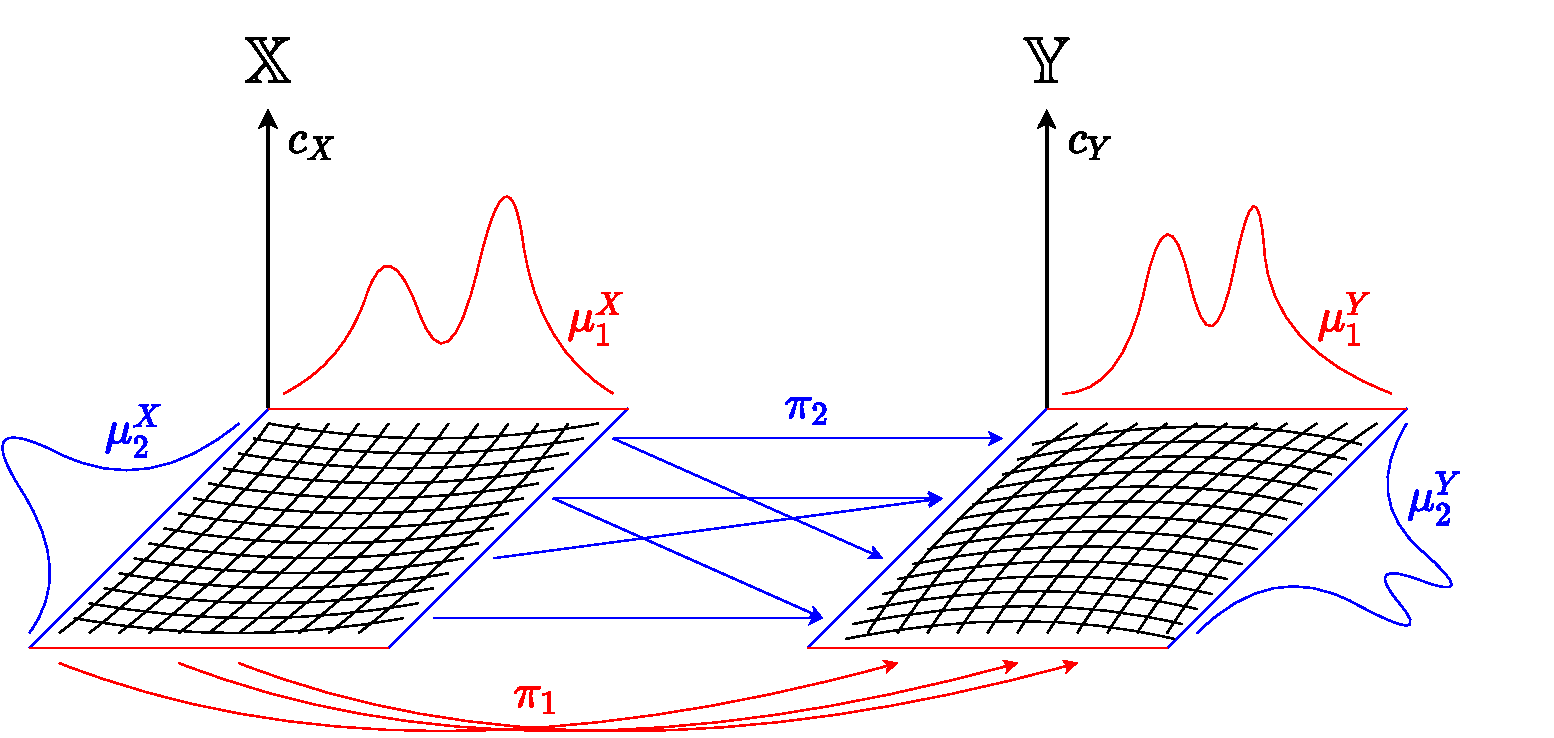
\includegraphics[width=0.9\textwidth, keepaspectratio]{./Chapitre2/fig/coot_diagram.pdf}
%   \caption{Scatter plots of MMOT-DC-v1 versus other solvers. In all three plots, the points tend to concentrate around the line $y=x$,
%   which indicates the comparable performance of MMOT-DC-v1. On the other hand, the top-right plot shows the clear superiority of EGW-PGD.}
%   \label{fig:continuous_coot}
% \end{figure}
First, we can show that the COOT problem \eqref{eq:cont_coot} is well defined.
\begin{proposition}[Lemma 35 in \citep{Chowdhury21b}]
  \label{prop:exist_coot}
  The COOT problem always admits a minimizer.
\end{proposition}
We provide the proof in Appendix \ref{annex:cont_coot}.
While the proofs of our result and of Lemma 35 in \citep{Chowdhury21b} use the same proof technique of
Theorem 2.2 in \citep{Chowdhury19}, ours is slightly different. More precisely,
we exploit a different reformulation of COOT, where it can be rewritten as a multi-marginal OT problem
with additional factorization constraint on the coupling. Later, we will see that,
this observation also allows to establish the convergence result of entropic COOT.

%%%%%%%%%%%%%%%%%%%%%%%%%%%%%%%%%%%%%%%%%%
\subsection{Metric properties}

The framework on the GW isomorphism presented in \Cref{subsec:prop_gw}
can be extended immediately to the COOT setting. In particular, while our
presentation is different to that of \citep{Chowdhury21b}, we still come up with the
same metric properties.

%%%%%%%%%%%%%%%%%%%%%%%%%%%%%%%%%%%%%%%%%
\begin{definition}[Relaxed mass splitting]
  A measure hypernetwork $\cZ$ is a \textbf{relaxed mass splitting} (RMS) of a
  measure hypernetwork $\cX$ if there exist two measure-preserving maps
  $\varphi_k: Z_k \to X_k$, for $k=1,2$, such that the pullback equality
  $c_Z = (\varphi_1, \varphi_2)^*c_X$ holds $\mu^Z_1 \otimes \mu_2^Z$-almost everywhere
  in $Z_1 \times Z_2$. We denote $\ms(\cX)$ the set of all mass splittings
  of $\cX$. This pair of maps $(\varphi_1, \varphi_2)$ is also called
  \textbf{basic weak isomorphism} in \citep{Chowdhury21b}.
\end{definition}
We denote $\rms(\cX)$ the set of all relaxed mass splittings of $\cX$. Clearly,
$\cX \in \rms(\cX)$, so $\rms(\cX)$ is not empty.
In particular, for measure networks, if $\cZ \in \ms(\cX)$, then $\cZ \in \rms(\cX)$,
meaning that $\ms(\cX) \subset \rms(\cX)$. Now, we can define the isomorphism between
the measure hypernetworks as follows.
\begin{definition}[COOT-isomorphism] \label{coot_isomorphic}
  Two measure hypernetworks are
  \begin{enumerate}
    \item strongly isomorphic if there exist two \textbf{bijective}
    measure-preserving map from one hypernetwork to the other such that the pullback equality holds
    \textbf{everywhere}.
    \item semi-strongly isomorphic if one is the RMS of the other and vice versa.
    \item weakly isomorphic if they have a common RMS.
  \end{enumerate}
\end{definition}
This is an immediate relaxation of the GW isomorphism. In particular,
in case of measure networks, isomorphism in GW sense implies COOT isormorphism.
The following result summarizes the relations amongst the three types of COOT isomorphism.
%%%%%%%%%%%%%%%%%%%%%%%%%%%%%%%%%%%%%%%%%%%%%%%%
\begin{corollary} \label{prop:strong_weak_iso}
  Given two measure hypernetworks $\cX$ and $\cY$. Consider three statements
  \begin{enumerate}
    \item[(1)] $\cX$ and $\cY$ are strongly isomorphism.
    \item[(2)] $\cX$ and $\cY$ are semi-strongly isomorphism.
    \item[(3)] $\cX$ and $\cY$ are weakly isomorphism.
  \end{enumerate}
  Then, the following relations hold
  \begin{enumerate}
    \item $(1) \implies (2) \implies (3)$.
    \item If $\cX$ and $\cY$ are finite, then $(2) \implies (1)$.
    \item If $\cX$ and $\cY$ are finite such that $|X_k| = |Y_k|$
    and $\mu_k^X, \mu_k^Y$ are uniform distributions, for $k = 1,2$, then
    $(3) \implies (2)$. This means all three forms are equivalent.
  \end{enumerate}
\end{corollary}
%%%%%%%%%%%%%%%%%%%%%%%%%%%%%%%%%%%%%%%%%%%%%%%%
Now, we can characterize the weak isomorphism by
\begin{proposition} \label{prop:coot_iso}
  Two measure hypernetworks $\cX$ and $\cY$ are COOT-weakly isomorphic if and only if
  $\coot(\cX, \cY) = 0$.
\end{proposition}
%%%%%%%%%%%%%%%%%%%%%%%%%%%%%%%%%%%%%%%%%%%%%%%%
\begin{proposition}[Theorem 1 in \citep{Chowdhury21b}] \label{prop:metric_prop}
  $\coot^{1/p}$ defines a metric on the space of measure hypernetworks, up to COOT-weak isomorphism.
\end{proposition}
%%%%%%%%%%%%%%%%%%%%%%%%%%%%%%%%%%%%%%%%%
% \paragraph{Discussion on the setting of mm-space}
% While the measure network can fit in the COOT framework, this is usually not the case for
% the mm-space since the distance function is only measurable in Polish space,
% but not necessarily bounded. However, all previous results on the existence of minimizer and
% metric property remain unchanged if one replaces measure hypernetworks by mm-spaces,
% as long as COOT is finite. Moreover,
% \begin{corollary}
% For $p=2$, all forms of COOT isomorphisms are equivalent and
% they are also equivalent to the isomorphism in GW sense.
% \end{corollary}
% This indicates that, both GW distance and COOT can be used to compare isometric objects,
% namely those transformed by reflection, rotation or translation.

%%%%%%%%%%%%%%%%%%%%%%%%%%%%%%%%%%%%%%%%%%%%%%%%
\subsection{Entropic regularization and approximation error}
%%%%%%%%%%%%%%%%%%%%%%%%%%%%%%%%%%%%%%%%%%%%%%%%
Similar to the Wasserstein and GW distances, one can approximate the COOT with entropic regularization.
In this thesis, we are interested in the following formulation of entropic COOT:
for $\varepsilon > 0$,
\begin{align}
  \coot_{\varepsilon} (\cX, \cY) =
  \inf_{\substack{\pi_1 \in U(\mu^X_1, \mu^Y_1) \\
  \pi_2 \in U(\mu^X_2, \mu^Y_2)}} &\iint
  \big\vert c_X(x_1, x_2) - c_Y(y_1, y_2) \big\vert^p \; d\pi_1(x_1, y_1) \; d\pi_2(x_2, y_2) \\
  &+ \varepsilon \; \kl \big( \pi_1 \otimes \pi_2 \vert (\mu^X_1 \otimes \mu^Y_1) \otimes (\mu^X_2 \otimes \mu^Y_2) \big).
\end{align}
Note that, this structure of the KL divergence term is particularly handy to prove all results related to
the entropic COOT. It also bears similarity with the \textit{quadratic divergence}
\citep{Sejourne20} defined by $\kl^{\otimes 2}(\mu, \nu):= \kl(\mu \otimes \mu | \nu \otimes \nu)$,
which is used to define the unbalanced GW divergence. Note that, in the balanced setting,
the joint penalization in terms of KL divergence is in fact equivalent to the
independent KL-penalization. More precisely, given any $\pi_k \in U(\mu_k^X, \mu_k^Y)$,
for $k=1,2$, we have
\begin{equation}
  \kl \big( \pi_1 \otimes \pi_2 \vert (\mu^X_1 \otimes \mu^Y_1) \otimes (\mu^X_2 \otimes \mu^Y_2) \big)
  = \kl(\pi_1 \vert \mu^X_1 \otimes \mu^Y_1) + \kl(\pi_2 \vert \mu^X_2 \otimes \mu^Y_2).
\end{equation}
In practice, since the couplings may not have the same nature (for example,
when working directly with the input data, rather than via the similarity matrix),
they can be penalized by different values of regularization.
%%%%%%%%%%%%%%%%%%%%%%%
\begin{proposition}
The entropic COOT problem always admits a minimizer.
\end{proposition}
%%%%%%%%%%%%%%%%%%%%%%%
One major practical interest of entropic COOT is that, for sufficiently small regularization,
it provides a good proxy for unregularized COOT. To formalize this observation, first,
we need to introduce the following assumption on the measure hypernetwork.
%%%%%%%%%%%%%%%%%%%%%%%%%%%%%
\begin{assumption}
  \label{assump:ent_coot}
  Given a measure hypernetwork, we assume that
  \begin{enumerate}
    \item[A1] The sample and feature spaces are finite-dimensional vector spaces.
    \item[A2] Their associated Borel probability measures are absolutely continuous
    with respect to the Lebesgue measure.
  \end{enumerate}
\end{assumption}
%%%%%%%%%%%%%%%%%%%%%%%%%%%%%%
\begin{proposition} \label{prop:conv_ent_coot}
  Under \Cref{assump:ent_coot}, if the interactions are continuous, then
  $\coot_{\varepsilon}(\cX, \cY) \to \coot(\cX, \cY)$ when $\varepsilon \to 0$. Moreover,
  let $(\varepsilon_n)_{n \in \bbN}$ be a sequence of
  positive regularizations such that $\varepsilon_n \to 0$.
  Denote $\pi_n := (\pi_{1, n}, \pi_{2, n})$ the solution of the entropic problem
  $\coot_{\varepsilon_n} (\cX, \cY)$. Then, any cluster point of the sequence $(\pi_n)_n$ is
  a solution of the unregularized COOT problem.
\end{proposition}
%%%%%%%%%%%%%%%%%%%%%%%%%%%%%%
The above result is similar to the one known in entropic OT \citep{Carlier17}. This is due to the fact
that the entropic COOT can be reformulated as a variant of multi-marginal OT problem,
thus the block approximation and $\Gamma$-convergence techniques can be applied.

Furthermore, still under \Cref{assump:ent_coot}, if the measure network is bounded,
then we can quantify the approximation error as follows.
%%%%%%%%%%%%%%%%%%%%%%%%%%%%%%
\begin{proposition} \label{prop:quant_bound_ent}
  Given two measure networks $\cX = (X, \mu_X, c_X)$ and $\cY = (Y, \mu_Y, c_Y)$.
  Suppose that $X$ is bounded subset of $\bbR^{d_x}$ and $Y$ is a bounded subset
  of $\bbR^{d_y}$, where $\diam(X), \diam(Y) \leq D$.
  Denote $d = \max(d_x, d_y)$. Suppose there exists a constants $q > 0$ such that
  $c_X(x_1, x_2) = \vert\vert x_1 - x_2 \vert\vert^q$, for every $(x_1,x_2) \in X^2$, and
  $c_Y(y_1, y_2) = \vert\vert y_1 - y_2 \vert\vert^q$, for every $(y_1,y_2) \in Y^2$. Then,
  \begin{equation}
    \coot_{\varepsilon}(\cX, \cY) - \coot(\cX, \cY) \leq
    \frac{2d \varepsilon}{pq} \log\Big( \frac{pq (2D d^{1/p})^{pq}}{2d \varepsilon} \Big).
  \end{equation}
\end{proposition}
%%%%%%%%%%%%%%%%%%%%%%%%%
This bound is very similar to the one in Wasserstein setting \citep{Genevay19}.
Let us consider two special cases of \Cref{prop:quant_bound_ent}.
\begin{itemize}
  \item[$\bullet$] When $p=2$ and $c_X, c_Y$ are Euclidean distances (\ie, $q=1$),
  the upper bound becomes $d\varepsilon \log\Big( \frac{4D^2}{\varepsilon} \Big)$.

  \item[$\bullet$] When $p=2$ and $c_X, c_Y$ are squared Euclidean distances
  (\ie, $q=2$), the upper bound becomes
  $\frac{d\varepsilon}{2} \log\Big( \frac{32dD^4}{\varepsilon} \Big)$.
\end{itemize}
In both situations, the dependence of the bound on the maximal distance $D$ between points
within each space (even only at logarithmic scale) and on the dimension $d$ indicates
that either high dimensional space, or large intra-space distance (for example, due to outliers)
can have negative impact on the approximation error. On the other hand,
by comparing these two bounds, we deduce that if $\log(2d \varepsilon) \leq 1$,
then the squared Euclidean distances generates a provably better (smaller) upper bound.

With little modification of the proof, exactly the same upper bound in \Cref{prop:quant_bound_ent}
holds for GW distance. We note that \citet{Zhang23} also establish a similar
$O(\varepsilon \log \varepsilon)$-approximation error between the unregularized and entropic GW,
but they rely on different assumptions to ours. In particular, their result only holds
for $2$-GW distance, when the distance function is the squared-Euclidean norm. By contrast,
\Cref{prop:quant_bound_ent} holds for any $p$-GW distance and any $L^q$-norm as distance function.

%%%%%%%%%%%%%%%%%%%%%%%%%%%%%%%%%%%%%%
\section{Factored couplings in Multi-marginal Optimal
Transport via Difference of Convex programming} \label{subsec:MMOT_DC}

%%%%%%%%%%%%%%%%%%%%%%%%%%%%%%%%%%%%%%%
\subsection{Introduction}

Broadly speaking, the classic OT problem provides a principled approach for transporting one probability distribution onto another
following the principle of the least effort. Such a problem, and the distance on the space of probability distributions derived from it,
arise in many areas of machine learning (ML) including generative modeling, transfer learning and information retrieval, where OT has
been successfully applied. A natural extension of classic OT, in which the admissible transport plan can have more
than two prescribed marginal distributions, is called the multi-marginal optimal transport (MMOT) \citep{Gangbo98}.
The latter has several attractive properties: it enjoys a duality theory \citep{Kellerer84} and finds connections with the
probabilistic graphical models \citep{Haasler20} and the Wasserstein barycenter problem \citep{Agueh11} used for data averaging.
While being less popular than the classic OT with two marginals, MMOT is a very useful framework on its own with some notable recent
applications in generative adversarial networks \citep{Cao19}, clustering \citep{Mi21} and domain adaptation
\citep{HuiLCHY18,HeZKSC19}, to name a few.

The recent success of OT in ML is often attributed to the entropic regularization \citep{Cuturi13} where the authors imposed a
constraint on the coupling matrix forcing it to be closer to the independent coupling given by the rank-one product of the marginals.
Such a constraint leads to the appearance of the strongly convex entropy term in the objective function and allows the entropic
OT problem to be solved efficiently using simple Sinkhorn-Knopp matrix balancing algorithm. In addition to this, it was also noticed
that structural constraints on the coupling and cost matrices allow to reduce the high computational cost and sample complexity
of the classic OT problem \citep{Genevay19,Forrow18,Chiheng21,Meyer21a}. However, none of these works considered a much more
challenging case of doing so in a multi-marginal setting. On the other hand, while the work of \citet{Haasler20} considers the MMOT
problem in which the cost tensor induced by a graphical structure, it does not naturally promote the factorizability of
transportation plans.

\paragraph{Contributions} In this work, we define and study a general MMOT problem with structural penalization on the coupling matrix.
We start by showing that a such formulation includes several popular OT methods as special cases and allows to gain deeper insights
into them. We further consider a relaxed problem where the hard constraint is replaced by a regularization term and show that it leads
to an instance of the difference of convex programming problem. A numerical study of the solutions obtained when solving the latter
in cases of interest highlights their competitive performance when compared to solutions provided by the optimization
strategies used previously.

%%%%%%%%%%%%%%%%%%%%%%%%%%%%%%%%%%%%%
\subsection{Preliminary knowledge}

\paragraph{Notations.} For each integer $n \geq 1$, we write $[n] := \{1,...,n\}$.
We denote $\langle \cdot, \cdot \rangle$ denotes the Frobenius inner product.
The generalized Kullback-Leibler divergence between two positive vectors $p, q \in \bbR^n_{> 0}$
is defined as $\kl(p | q) = \sum_i p_i \log \frac{p_i}{q_i} - \sum_i p_i + \sum_i q_i$,
with the convention that $0 \log 0 = 0$.

In what follows, given an integer $N \geq 1$, for any positive integers $a_1,..., a_N$, we call
$P \in \bbR^{a_1 \times ... \times a_N}$ a $N$-D tensor. In particular, a $1$-D tensor is a vector and $2$-D tensor is a matrix.
A tensor is a probability tensor if its entries are nonnegative and the sum of all entries is $1$.
Given $N$ probability vectors $\mu_1, ..., \mu_N$, we write $\mu = (\mu_n)_{n=1}^N$
and $\mu^{\otimes} := \mu_1 \otimes ... \otimes \mu_N$.
We denote $\Sigma$ the set of $N$-D probability tensors and $U(\mu) \subset \Sigma$ the set of nonnegative tensors whose $N$
marginal distributions are $\mu_1, ..., \mu_N$. In this case, any coupling in $U(\mu)$ is said to be \textit{admissible}.

\paragraph{Multi-marginal OT problem.} Given a collection of $N$ probability vectors $\mu = (\mu_n \in \bbR^{a_n})_{n=1}^N$
and a $N$-D cost tensor $C \in \bbR^{a_1 \times ... \times a_N}$, the MMOT problem reads
\begin{equation*}
  \mmot(\mu) = \inf_{P \in U(\mu)} \langle C, P \rangle.
\end{equation*}
In practice, such a formulation is intractable to optimize in a discrete setting as it results in a linear program where the number
of constraints grows exponentially in $N$. A more tractable strategy for solving MMOT is to consider the following entropic
regularization problem
\begin{equation} \label{MMOT_primal}
  \inf_{P \in U(\mu)} \langle C, P \rangle + \varepsilon \kl(P | \mu^{\otimes}).
\end{equation}
which can be solved using Sinkhorn's algorithm \citep{Benamou14}.
We refer the interested reader to Appendix \ref{appendix:subsec_mmot_dc} for algorithmic details.

%%%%%%%%%%%%%%%%%%%%%%%%%%%%%%%%%%%%%%%%%%%%%%%%%
\subsection{Factored Multi-marginal Optimal Transport}

In this section, we first define a factored MMOT (F-MMOT) problem where we seek to promote a structure on the optimal coupling
given such as a factorization into a tensor product. Interestingly, such a formulation can be shown to include several other
OT problems as special cases. Then, we introduce a relaxed version called MMOT-DC where the factorization constraint is
smoothly promoted through a Kullback-Leibler penalty.

\subsubsection{Motivation}

Before a formal statement of our problem, we first give a couple of motivating examples showing
why and when structural constraints on the coupling matrix can be beneficial. To this end,
first note that a trivial example of the usefulness of such constraints in OT is the famous
entropic regularization. Indeed, while most of the works define the latter by adding
negative entropy of the coupling to the classic OT objective function directly,
the original idea was to constraint the sought coupling to remain close (to some extent)
to a rank-one product of the two marginal distributions. The appearance of negative entropy
in the final objective function is then only a byproduct of such constraint due to
the decomposition of the KL divergence into a sum of three terms with two of them being constant.
Below we give two more examples of real-world applications related to MMOT problem
where a certain decomposition imposed on the coupling tensor can be desirable.
\paragraph{Multi-source multi-target translation.} A popular task in computer vision is
to match images across different domains in order to perform the so-called image translation.
Such tasks are often tackled within the GAN framework where one source domain from which
the translation is performed, is matched with multiple target domains modeled using generators.
While MMOT was applied in this context by \citet{Cao19} when only one source was considered,
its application in a multi-source setting may benefit from structural constraints
on the coupling tensor incorporating the human prior on what target domains each source domain
should be matched to.

\paragraph{Multi-task reinforcement learning.} In this application, the goal is to learn
individual policies for a set of agents while taking into account the similarities between them
and hoping that the latter will improve the individual policies. A common approach is
to consider an objective function consisting of two terms where the first term is concerned
with learning individual policies, while the second forces a consensus between them.
Similar to the example considered above, MMOT problem was used to promote the consensus
across different agents' policies in \citep{Cohen21}, even though such a consensus
could have benefited from a prior regarding the semantic relationships between the learned tasks.
%
%We can cite other examples motivating the introduction of structural constraints in MMOT problem but the bottom line of it remains unchanged: imposing a certain structure on the optimal coupling tensor is a way of incorporating the human-based priors to the MMOT problem that reflect the domain knowledge about the problem at hand. We now proceed to the formal introduction of this idea.

\subsubsection{Factored MMOT and its relaxation}
We start by giving several definitions used in the following parts of this section.
%We call $P \in \bbR^{a_1 \times ... \times a_N}$ a $N$-D tensor. When $N=1$, we simply call it a vector and when $N=2$,
%it is a matrix.
\begin{definition}[Tuple partition]
 Given two integers $N \geq M \geq 2$, a sequence of tuples $\cT = (\cT_m)_{m=1}^M$, is called a
 \underline{tuple partition} of the $N$-tuple $(1,...,N)$ if the tuples $\cT_1, ..., \cT_M$ are nonempty and disjoint,
 and their concatenation in this order gives $(1,...,N)$.
\end{definition}
Here, we implicitly take into account the order of the tuple, which is not the case for the partition of the set $[N]$. If
there exists a tuple in $\cT$ which contains only one element, then we say $\cT$ is \textit{degenerate}.

\begin{definition}[Marginal tensor]
  Given a tensor $P \in \bbR^{a_1 \times ... \times a_N}$ and a tuple partition $\cT = (\cT_m)_{m=1}^M$,
  we call $P_{\# \cT_m}$ its \underline{$\cT_m$-marginal tensor}, by summing $P$ over all dimensions not in $\cT_m$.
  We write $P_{\# \cT} = P_{\# \cT_1} \otimes ... \otimes P_{\# \cT_M} \in \bbR^{a_1 \times ... \times a_N}$
  the tensor product of its marginal tensors.
\end{definition}
For example, for $M=N=2$, we have $\cT_1 = (1)$ and $\cT_2 = (2)$. So, given a matrix
$P \in \bbR^{a_1 \times a_2}$, its marginal tensors $P_{\# \cT_1}$ and $P_{\# \cT_2}$ are simply vectors in
$\bbR^{a_1}$ and $\bbR^{a_2}$, respectively, defined by $(P_{\# \cT_1})_i = \sum_j P_{ij}$ and
$(P_{\# \cT_2})_j = \sum_i P_{ij}$ for $(i,j) \in [a_1] \times [a_2]$. The tensor product
$P_{\# \cT} \in \bbR^{a_1 \times a_2}$ is then defined by
$(P_{\#\cT})_{ij} = (P_{\# \cT_1})_i (P_{\# \cT_2})_j$.
Clearly, if $P$ is a probability tensor, then so are its marginal tensors and tensor product.

Suppose $\cT_m = (p,...,q)$ for some $m \in [M]$ and $1 \leq p \leq q \leq N$. We denote
$\Sigma_{\cT_m}$ the set of probability tensors in $\bbR^{a_p \times ... \times a_q}$ and
$U_{\cT_m} \subset \Sigma_{\cT_m}$ the set
of probability tensors in $\bbR^{a_p \times ... \times a_q}$ whose
$r^{\text{th}}$-marginal vector is $\mu_r$, for every $r = p,...,q$.
We also define $\mu^{\otimes}_{\cT_m} := \mu_p \otimes ... \otimes \mu_q$.

%%%%%%%%%%%%%%%%%%%%%%%%%%%%%%%
\begin{definition}[Factored MMOT]
  Given a collection of histograms $\mu = (\mu_n)_{n=1}^N$ and a tuple partition $\cT = (\cT_m)_{m=1}^M$,
  we consider the following OT problem
  \begin{equation} \label{factor_mmot}
    \fmmot( \cT, \mu) = \inf_{P \in U_{\cT}} \langle C, P \rangle,
  \end{equation}
  where $U_{\cT} \subset U(\mu)$ is the set of admissible couplings which can be factorized as a tensor product of $M$
  component probability tensors in $\Sigma_{\cT_1}, ..., \Sigma_{\cT_M}$.
\end{definition}
Several remarks are in order here. First, one should note that the partition considered above is in general not degenerate meaning
that the decomposition can involve tensors of an arbitrary order $<N$. Second, the decomposition in this setting depicts the prior
knowledge regarding the tuples of measures which should be independent: the couplings for the measures from different tuples will
be degenerate and the optimal coupling tensor will be reconstructed from couplings of each tuple separately.
Third, suppose the partition $(\cT_m)_{m=1}^M$ is not degenerate and $M=2$, i.e. the tensor is factorized as product of
two tensors, Problem \eqref{factor_mmot} is equivalent to a variation of low non-negative rank OT problem
(see Appendix \ref{appendix:subsec_mmot_dc}).

As for the existence of the solution to this problem, we have that $U_{\cT}$ is compact because it is a close subset of the
compact set $U(\mu)$, which implies that Problem \eqref{factor_mmot} always admits a solution. Furthermore, observe that
\begin{equation}
  \begin{split}
    U_{\cT} &= \{ P \in U(\mu): P = P_1 \otimes ... \otimes P_M, \text{where } P_m \in \Sigma_{\cT_m}, \forall m = 1,...,M \} \\
    &= \{ P \in \Sigma: P = P_1 \otimes ... \otimes P_M, \text{where } P_m \in U_{\cT_m}, \forall m = 1,...,M \}.
  \end{split}
\end{equation}
Thus, the problem F-MMOT can be rewritten as
\begin{equation}
  \fmmot( \cT, \mu) = \inf_{\substack{P_m \in U_{\cT_m} \\ \forall m = 1,...,M}}
  \langle C, P_1 \otimes ... \otimes P_M \rangle.
\end{equation}
So, if $\cT_1,...,\cT_M$ are $2$-tuples and two marginal distributions corresponding to each $U_{\cT_m}$ are
identical and uniform, then by Birkhoff's theorem \citep{Birkhoff46}, Problem \eqref{factor_mmot} admits an optimal solution in
which each component tensor $P_m$ is a permutation matrix.

\paragraph{Two special cases.} When $N = 4$ and $M=2$ with $\cT_1 = (1,2)$ and $\cT_2 = (3,4)$, Problem
\eqref{factor_mmot} becomes the CO-Optimal transport (COOT), where the two component tensors are known as
\textit{sample} and \textit{feature} couplings. If furthermore, $a_1 = a_3, a_2=a_4$, and $\mu_1 = \mu_3, \mu_2=\mu_4$, it becomes a
lower bound of the discrete Gromov-Wasserstein (GW) distance. This means that our formulation can be seen as a
generalization of several OT formulations.

%%%%%%%%%%%%%%%%%%%%%%%%%%%%%%%%%%%%%%%%%%%%%
Observe that if a probability tensor $P$ can be factorized as a tensor product of probability tensors, i.e.
$P = P_1 \otimes ... \otimes P_M$, then each $P_m$ is also the $\cT_m$-marginal tensor of $P$. In this case,
we have $P = P_{\# \cT}$. This prompts us to consider the following relaxation of factored MMOT, where the hard constraint
$U_{\cT}$ is replaced by a regularization term.
\begin{definition}[Relaxed Factored MMOT]
  Given $\varepsilon \geq 0$, a collection of measures $\mu$ and a tuple partition $\cT$,
  we define the following problem:
  \begin{equation} \label{relax_mmot}
    \mmotdc_{\varepsilon}( \cT, \mu) =
    \inf_{P \in U(\mu)} \langle C, P \rangle + \varepsilon \kl(P \vert P_{\# \cT}).
  \end{equation}
\end{definition}
From the exposition above, one can guess that this relaxation is reminiscent of the entropic regularization in MMOT and
coincides with it when $M = N$. As such, it also recovers the classical entropic OT. One should note that the choice of the KL
divergence is not arbitrary and its advantage will become clear when it comes to the algorithm. %A well known
A special case of Problem \eqref{relax_mmot} is when $M = N$, we recover the entropic-regularized MMOT problem.

After having defined the two optimization problems, we now set on exploring their theoretical properties.

%%%%%%%%%%%%%%%%%%%%%%%%%%%%%%%%%%%%%%%%%%%%%%%
\subsection{Theoretical properties}
Intuitively, the relaxed problem is expected to allow for solutions with a lower value of the final objective function. We formally prove the validity of this intuition below.
%%%%%%%%%%%%%%%%%%%%%%%%%%%%%%%%%%%%%%%%%%%%%
\begin{proposition}[Preliminary properties]
  \label{MMOT_dc_prop}
  Given a collection of histograms $\mu$ and a tuple partition $\cT$,
  \begin{enumerate}
    \item For every $\varepsilon \geq 0$, we have $\mmot(\mu) \leq
    \mmotdc_{\varepsilon}(\cT, \mu) \leq \fmmot( \cT, \mu)$.
    \item For every $\varepsilon > 0, \mmotdc_{\varepsilon}( \cT, \mu ) = 0$ if and only if
    $\fmmot (\cT, \mu) = 0$.
  \end{enumerate}
\end{proposition}
%%%%%%%%%%%%%%%%%%%%%%%%%%%%%%%%%%%%%%%%%%%%%
An interesting property of MMOT-DC is that it interpolates between MMOT and F-MMOT. Informally,
for very large $\varepsilon$, the KL divergence term dominates, so the optimal transport plans tend to be factorizable.
On the other hand, for very small $\varepsilon$, the KL divergence term becomes negligible and we approach MMOT.
The result below formalizes this intuition.
%%%%%%%%%%%%%%%%%%%%%%%%%%%%%%%%%%%%%%%%%%%%%
\begin{proposition}[Interpolation between MMOT and F-MMOT]
  \label{interpolation_prop}
  For any tuple partition $\cT$ and for $\varepsilon > 0$,
  let $P_{\varepsilon}$ be a minimiser of the problem $\mmotdc_{\varepsilon}(\cT, \mu)$.
  \begin{enumerate}
    \item When $\varepsilon \to \infty$, one has $\mmotdc_{\varepsilon}(\cT, \mu) \to
    \fmmot(\cT, \mu)$. In this case, any cluster point of the sequence of minimisers
    $(P_{\varepsilon})_{\varepsilon}$ is a minimiser of $\fmmot(\cT, \mu)$.

    \item When $\varepsilon \to 0$, then $\mmotdc_{\varepsilon}(\cT, \mu) \to \mmot(\mu)$.
    In this case, any cluster point of the sequence of minimisers $(P_{\varepsilon})_{\varepsilon}$ is a minimiser of
    $\mmot(\mu)$.
  \end{enumerate}
\end{proposition}
%%%%%%%%%%%%%%%%%%%%%%%%%%%%%%%%%%%%%%%%%%%%%
\paragraph{GW distance revisited.} Somewhat surprisingly, the relaxation \eqref{relax_mmot} also allows us to prove the equality
between GW distance and COOT in the discrete setting. Let $\cX$ be a
finite subset (of size $m$) of a certain metric space. Denote $C_x \in \bbR^{m \times m}$ its similarity matrix (e.g. distance
matrix). We define similarly the set $\cY$ of size $n$ and the corresponding similarity matrix $C_y \in \bbR^{n \times n}$.
We also assign two discrete probability measures $\mu_x \in \bbR^m$ and $\mu_y \in \bbR^n$ to $\cX$ and $\cY$,
respectively. The GW distance is then defined as
\begin{equation}
  \gw(C_x, C_y) = \inf_{Q \in U(\mu_x, \mu_y)} \langle L(C_x, C_y), Q \otimes Q \rangle,
\end{equation}
and the COOT reads
\begin{equation}
  \coot(C_x, C_y) = \inf_{\substack{Q_s \in U(\mu_x, \mu_y) \\ Q_f \in U(\mu_x, \mu_y)}}
  \langle L(C_x, C_y), Q_s \otimes Q_f \rangle,
\end{equation}
where $L(C_x,C_y) \in \bbR^{m \times n \times m \times n}$ represents the $4$-D cost tensor induced by the matrices $C_x$ and $C_y$,
and $U(\mu, \nu)$ is the set of couplings in $\bbR^{m \times n}_{\geq 0}$ whose two marginal distributions are $\mu$ and
$\nu$. When $C_x$ and $C_y$ are two squared Euclidean distance matrices, and $L(C_x,C_y)$ is of the form
$\big(L(C_x,C_y)\big)_{i,j,k,l} = \vert (C_x)_{i,k} - (C_y)_{j,l} \vert^2$, it can be shown that the GW distance is equal
to the COOT. This is also true when $L(C_x, C_y)$ is a negative definite kernel \citep{Sejourne20}.
Here, we establish a weaker case where this equality still holds.
%%%%%%%%%%%%%%%%%%%%%%%%%%%%%%%%%%%%%%%%%%%%%
\begin{corollary} \label{kernel_gw_coot}
  If $L(C_x, C_y)$ defines a conditionally negative definite kernel on $(\cX \times \cY)^2$, then we have the equality
  between GW distance and COOT. Furthermore, if $(Q_s^*,Q_f^*)$ is a solution of the COOT problem, then $Q_s^*$ and $Q_f^*$ are
  two solutions of the GW problem. In particular, when $L(C_x, C_y)$ induces a strictly positive definite kernel
  $\exp \big( -\frac{L(C_x, C_y)}{\varepsilon} \big)$, for every $\varepsilon > 0$, we have $Q_s^* = Q_f^*$.
\end{corollary}
%%%%%%%%%%%%%%%%%%%%%%%%%%%%%%%%%%%%%%%%%%%%%
The proof relies on the connection between MMOT-DC and COOT shown in \Cref{interpolation_prop},
and given a $4$-D solution of MMOT-DC, we can construct another $4$-D solutions whose
$\cT_1$ and $\cT_2$-marginal matrices are identical,
under the assumption of the cost tensor. The proof of the second claim is deferred to the
Appendix \ref{appendix:subsec_mmot_dc}.

%%%%%%%%%%%%%%%%%%%%%%%%%%%%%%%%%%%%%%%%%%%%%%%%%%%%%ù
\subsection{Numerical solution} \label{sec:algo}
%%%%%%%%%%%%%%%%%%%%%%%%%%%%%%%%%%%%%%%%%%%%%
We now turn to the computational aspect of Problem \eqref{relax_mmot}. First, note that for any tuple partition
$\cT = (\cT_m)_{m=1}^M$ and probability tensor $P$, the KL divergence term can be decomposed as
\begin{equation}
  \kl(P \vert P_{\# \cT}) = \kl(P | \mu^{\otimes}) - \sum_{m=1}^m \kl_m(P),
\end{equation}
where the function $\kl_m$ defined by $\kl_m(P) := \kl(P_{\# \cT_m} | \mu^{\otimes}_{\cT_m})$
is continuous and convex with respect to $P$. Now, Problem \eqref{relax_mmot} becomes
\begin{equation} \label{relax}
  \mmotdc_{\varepsilon}(\cT, \mu) = \inf_{P \in U(\mu)}
  \langle C, P \rangle + \varepsilon \kl(P | \mu^{\otimes}) - \varepsilon \sum_{m=1}^m \kl_m(P).
\end{equation}
This is nothing but a Difference of Convex (DC) programming problem (which explains the name MMOT-DC),
thanks to the convexity of the set $U(\mu)$ and the KL divergence. Thus, it can be solved
by the classic DC algorithm
\footnote{The DC algorithm is very closely related to Convex-concave procedure,
majorization-minimization algorithm, Successive Linear
Approximation. See \citep{Le18} for more details.} \citep{Tao86,Tao97} as follows:
at the iteration $t$,
\begin{enumerate}
  \item Calculate $G^{(t)} \in \partial(\sum_{m=1}^M \kl_m)(P^{(t)})$.
  \item Solve $P^{(t+1)} \in \argmin_{P \in U(\mu)} \langle C -
  \varepsilon G^{(t)}, P \rangle + \varepsilon \kl(P | \mu^{\otimes})$.
\end{enumerate}
%%%%%%%%%%%%%%%%%%%%%%%%%%%%%%%%%%%%%%%%%%%%%%
This algorithm is very easy to implement. Indeed, the second step is an entropic-regularized MMOT problem, which admits a unique
solution, thanks to the strict convexity of the objective function.
Such solution can be found by the Sinkhorn algorithm
\ref{algo:dual_mmot}. In the first step, the gradient can be calculated explicitly.
For the sake of simplicity, we illustrate the calculation in a simple case, where $M=2$ and $N=4$ with
$\cT_1$ and $\cT_2$ are two $2$-tuples. The function $\kl_1 + \kl_2$ is continuous, so
$G^{(t)} = \nabla_P (\kl_1 + \kl_2)(P^{(t)})$. Given a $4$-D probability tensor $P$, we have
\begin{equation} \label{optim_condition}
  \frac{\partial (\kl_1 + \kl_2)}{\partial P_{i,j,k,l}} =
  \log \left( \frac{\sum_{k,l} P_{i,j,k,l}}{(\mu_1)_i (\mu_2)_j} \right) +
  \log \left( \frac{\sum_{i,j} P_{i,j,k,l}}{(\mu_3)_k (\mu_4)_l} \right).
\end{equation}
The complete DC algorithm for Problem \eqref{relax} can be found in \Cref{algo:dc_MMOT}.
%%%%%%%%%%%%%%%%%%%%%%%%%%%%%%%%%%%%%%%%%%%%%%
\begin{algorithm}[t]
  \caption{DC algorithm for Problem \eqref{relax_mmot}.}
  \textbf{Input.} Cost tensor $C$, tuple partition $(\cT_m)_{m=1}^M$, collection of histograms $\mu = (\mu_n)_{n=1}^N$,
  hyperparameter $\varepsilon > 0$, initialization $P^{(0)}$, tuple of initial dual vectors for the
  Sinkhorn step $(f_1^{(0)},...,f_N^{(0)})$.

  \textbf{Output.} Tensor $P \in U(\mu)$.

  While not converge
  \begin{enumerate}
    \item Gradient step: compute the gradient of the convex term $G^{(t)} = \sum\limits_{m=1}^M \nabla_P \kl_m(P^{(t)})$.
    \item Sinkhorn step: solve
    \begin{equation}
      P^{(t+1)} = \argmin_{P \in U(\mu)} \langle C - \varepsilon G^{(t)}, P \rangle + \varepsilon \kl(P | \mu^{\otimes}),
    \end{equation}
    using the Sinkhorn algorithm \ref{algo:dual_mmot}, with the tuple of initial dual vectors $(f_1^{(0)},...,f_N^{(0)})$.
  \end{enumerate}
  \label{algo:dc_MMOT}
\end{algorithm}

%%%%%%%%%%%%%%%%%%%%%%%%%%%%%%%%%%%%%%%%%%%%%%
\subsection{Experimental evaluation} \label{sec:exp}
%%%%%%%%%%%%%%%%%%%%%%%%%%%%%%%%%%%%%%%%%%%%%%
In this section, we illustrate the use of MMOT-DC on simulated data. Rather than performing experiments in full generality,
we choose the setting where $N = 4$ and $M=2$ with $\cT_1 = (1,2)$ and $\cT_2 = (3,4)$,
so that we can compare MMOT-DC with other popular solvers of COOT and GW distance. Given two matrices $X$ and $Y$, we always consider the $4$-D cost tensor $C$,
where $C_{i,j,k,l} = \vert X_{i,k} - Y_{j,l} \vert^2$. On the other hand, we are not interested in the $4$-D minimiser of MMOT-DC,
but only in its two $\cT_1, \cT_2$-marginal matrices.

\paragraph{Solving COOT on a toy example.} We generate a random matrix $X \in \bbR^{30 \times 25}$, whose entries are drawn independently
from the uniform distribution on the interval $[0,1)$. We equip the rows and columns of $X$ with two discrete uniform distributions
on $[30]$ and $[25]$. We fix two permutation matrices $Q_s \in \bbR^{30 \times 30}$ (called sample permutation) and
$Q_f \in \bbR^{25 \times 25}$ (called feature permutation), then calculate $Y = Q_s X Q_f$. We also equip the rows and columns of $Y$
with two discrete uniform distributions on $[30]$ and $[25]$.

It is not difficult to see that $\coot(X,Y) = 0$ because $(Q_s, Q_f)$ is a solution. As COOT is a special case of F-MMOT,
we see that $\mmotdc_{\varepsilon}(\cT, \mu) = 0$, for every $\varepsilon > 0$,
by \Cref{MMOT_dc_prop}. In this experiment, we will check if marginalizing the minimizer of MMOT-DC allows us to recover
the permutation matrices $Q_s$ and $Q_f$.
As can be seen from \Cref{fig:permu}, MMOT-DC can recover the permutation positions, for various
values of $\varepsilon$. On the other hand, it can not recover the true sparse permutation matrices because the Sinkhorn algorithm
applied to the MMOT problem implicitly results in a dense tensor, thus having dense marginal matrices. For this reason,
the loss only remains very close to zero, but never exactly.
%%%%%%%%%%%%%%%%%%%%%%%%%%%%%%%%%%%%%%%
\begin{figure}[t]
  \centering
  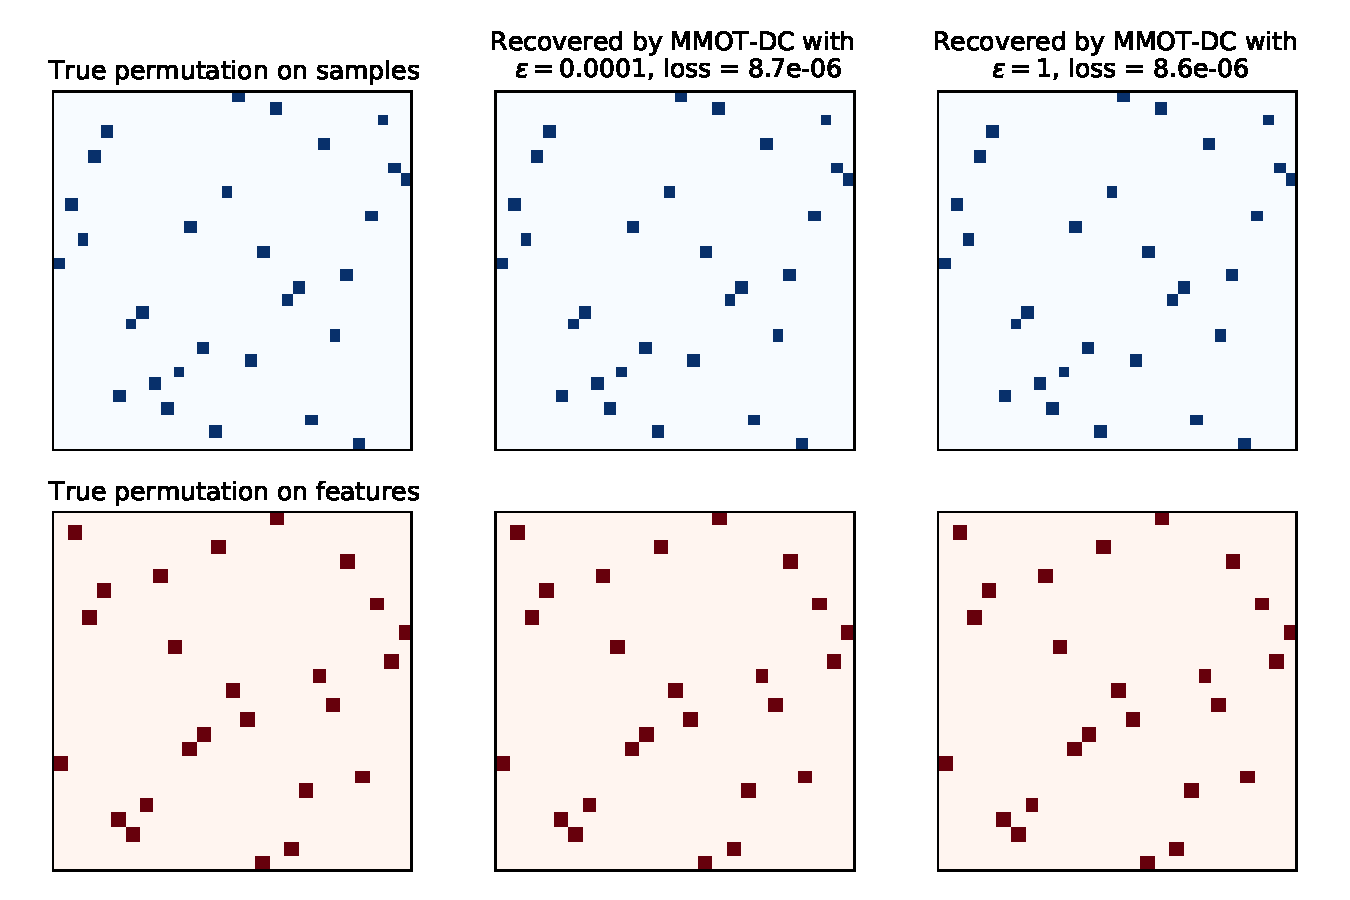
\includegraphics[width=0.8\textwidth,height=0.8\textheight,keepaspectratio]{./Chapitre2/fig/compare_methods.pdf}
  \caption{Couplings generated by COOT and MMOT-DC on the matrix recovering task.}
  \label{fig:permu}
\end{figure}
%%%%%%%%%%%%%%%%%%%%%%%%%%%%%%%%%%%%%%%
We also plot, with some abuse of notation, the histograms of the difference between
the $(1,3), (1,4), (2,3), (2,4)$-marginal matrices of MMOT-DC and their corresponding counterparts from F-MMOT.
In this example, in theory, as the optimal tensor $P$ of F-MMOT can be factorized as
$P = P_{\# \cT_1} \otimes P_{\# \cT_2} = Q_s \otimes Q_f$,
it is immediate to see that $P_{\# (1,3)} = P_{\# (1,4)} = P_{\# (2,3)} = P_{\# (2,4)} \in \bbR^{30 \times 25}$
are uniform matrices whose entries are $\frac{1}{750}$.
%%%%%%%%%%%%%%%%%%%%%%%%%%%%%%%%%%%%%%%
\begin{figure}[t]
  \centering
  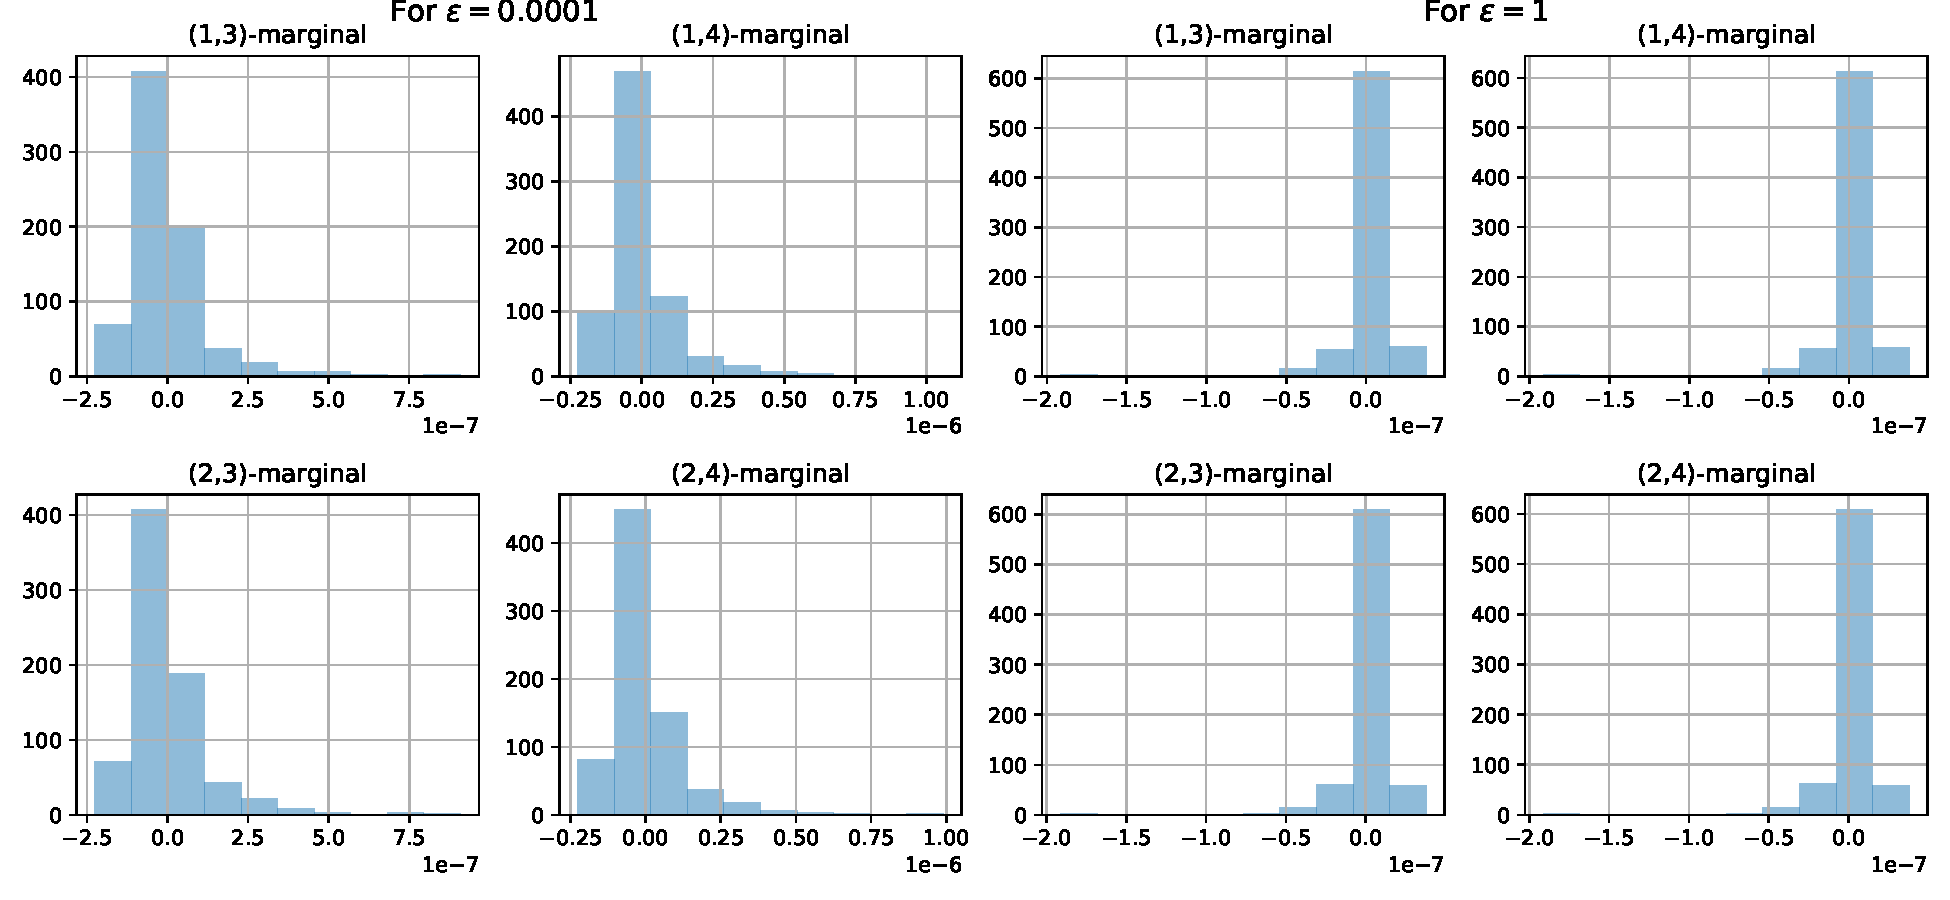
\includegraphics[width=1.\textwidth,height=1.\textheight,keepaspectratio]{./Chapitre2/fig/other_marginals.pdf}
  \caption{Histograms of difference between true independent marginal matrices and their approximations. We see that the marginal matrices obtained
  by \Cref{algo:dc_MMOT} approximate well the theoretical uniform matrices.}
  \label{fig:other_marg}
\end{figure}

%%%%%%%%%%%%%%%%%%%%%%%%%%%%%%%%%%%%%%%
\paragraph{Quality of the MMOT-DC solutions. \label{expe:2}}

% In the following example, our evaluation metric is the COOT loss $\langle C, P \otimes Q \rangle$,
% where the smaller the loss, the better.

Now, we consider the situation where the true matching between two matrices is not known in advance and investigate the quality
of the solutions returned by MMOT-DC to solve the COOT and GW problems. This means that we will look at the COOT loss
$\langle C, Q_s \otimes Q_f \rangle$, where the smaller the loss, the better when using both exact COOT and GW solvers
and our relaxation.

We generate two random matrices $X \in \bbR^{20 \times 3}$ and $Y \in \bbR^{30 \times 2}$,
whose entries are drawn independently from the uniform distribution on the interval $[0,1)$. Then we calculate two corresponding
squared Euclidean distance matrices of size $20$ and $30$. Their rows and columns are equipped with the discrete
uniform distributions. In this case, \citet{Redko20} show that the COOT loss coincides with the GW distance, and the
Block Coordinate Descent (BCD) algorithm used to approximate COOT is equivalent to the Frank-Wolfe algorithm \citep{Frank56}
used to solve the GW distance.

We compare four solvers:
\begin{enumerate}
  \item The Frank-Wolfe algorithm to solve the GW distance (GW-FW).

  \item The projected gradient algorithm to solve the entropic GW distance \citep{Peyre16} (EGW-PGD).
  We choose the regularization parameter from the set
  $\{0.0008, 0.0016, 0.0032, 0.0064, 0.0128, 0.0256 \}$
  and pick the one which corresponds to smallest COOT loss.

  \item The Block Coordinate Descent algorithm to approximate the entropic COOT \citep{Redko20}
  (EGW-BCD), where two additional KL divergences corresponding to two couplings are introduced.

  The regularization parameters are tuned from the set
  $\{0, 0.0005, 0.001, 0.005, 0.01, 0.05, 0.1, 0.5, 1 \}$,
  where $0$ means that there is no regularization term for the corresponding coupling
  and we pick the pair corresponding to the smallest COOT loss.

  \item \Cref{algo:dc_MMOT} to solve the MMOT-DC. We tune
  $\varepsilon \in \{1, 1.4, 1.8, 2.2, 2.6\}$ and we pick the one which corresponds to smallest COOT loss.
\end{enumerate}
For GW-FW and EGW-PGD, we use the implementation from the Python Optimal Transport package \citep{Flamary21}.

Given two random matrices, we record the COOT loss corresponding to the solution generated by each method.
We simulate this process $70$ times and compare their overall performance. We can see in \Cref{tab:gw} the average value and
standard deviation and the comparison for the values of the loss between the different algorithms in \Cref{fig:gw}.
The performance is quite similar across methods with a  slight advantage for EGW-PGD. This is in itself a very
interesting result that has never been noted, to the best of our knowledge: the reason that the entropic version of GW can
provide better solution than solving the exact problem, may be due to the "convexification" of the problem, thanks to the entropic
regularization. Our approach is also interestingly better than the exact GW-FW, which illustrates that the relaxation might help in
finding better solutions despite the non-convexity of the problem.
%%%%%%%%%%%%%%%%%%%%%%%%%%%%%%%%%%%%%%%
\begin{table}[t]
  % \vskip 0.15in
  \begin{center}
    \begin{small}
      \begin{sc}
        \begin{tabular}{|c|c|c|c|}
          \hline
          GW-FW & EGW-PGD & EGW-BCD & MMOT-DC \\
          \hline
          0.0829 ($\pm$ 0.0354) & \textbf{0.0786 ($\pm$ 0.0347)} & 0.0804 ($\pm$ 0.0353) & 0.0822 ($\pm$ 0.0364) \\
          \hline
        \end{tabular}
      \end{sc}
    \end{small}
  \end{center}
  \caption{Average and standard deviation of COOT loss of the solvers. MMOT-DC is competitive to other solvers,
  except for EGW-PGD and EGW-BCD.
  \label{tab:gw}}
\end{table}

%%%%%%%%%%%%%%%%%%%%%%%%%%%%%%%%%%%%%%%
\begin{figure}[t]
	\centering
	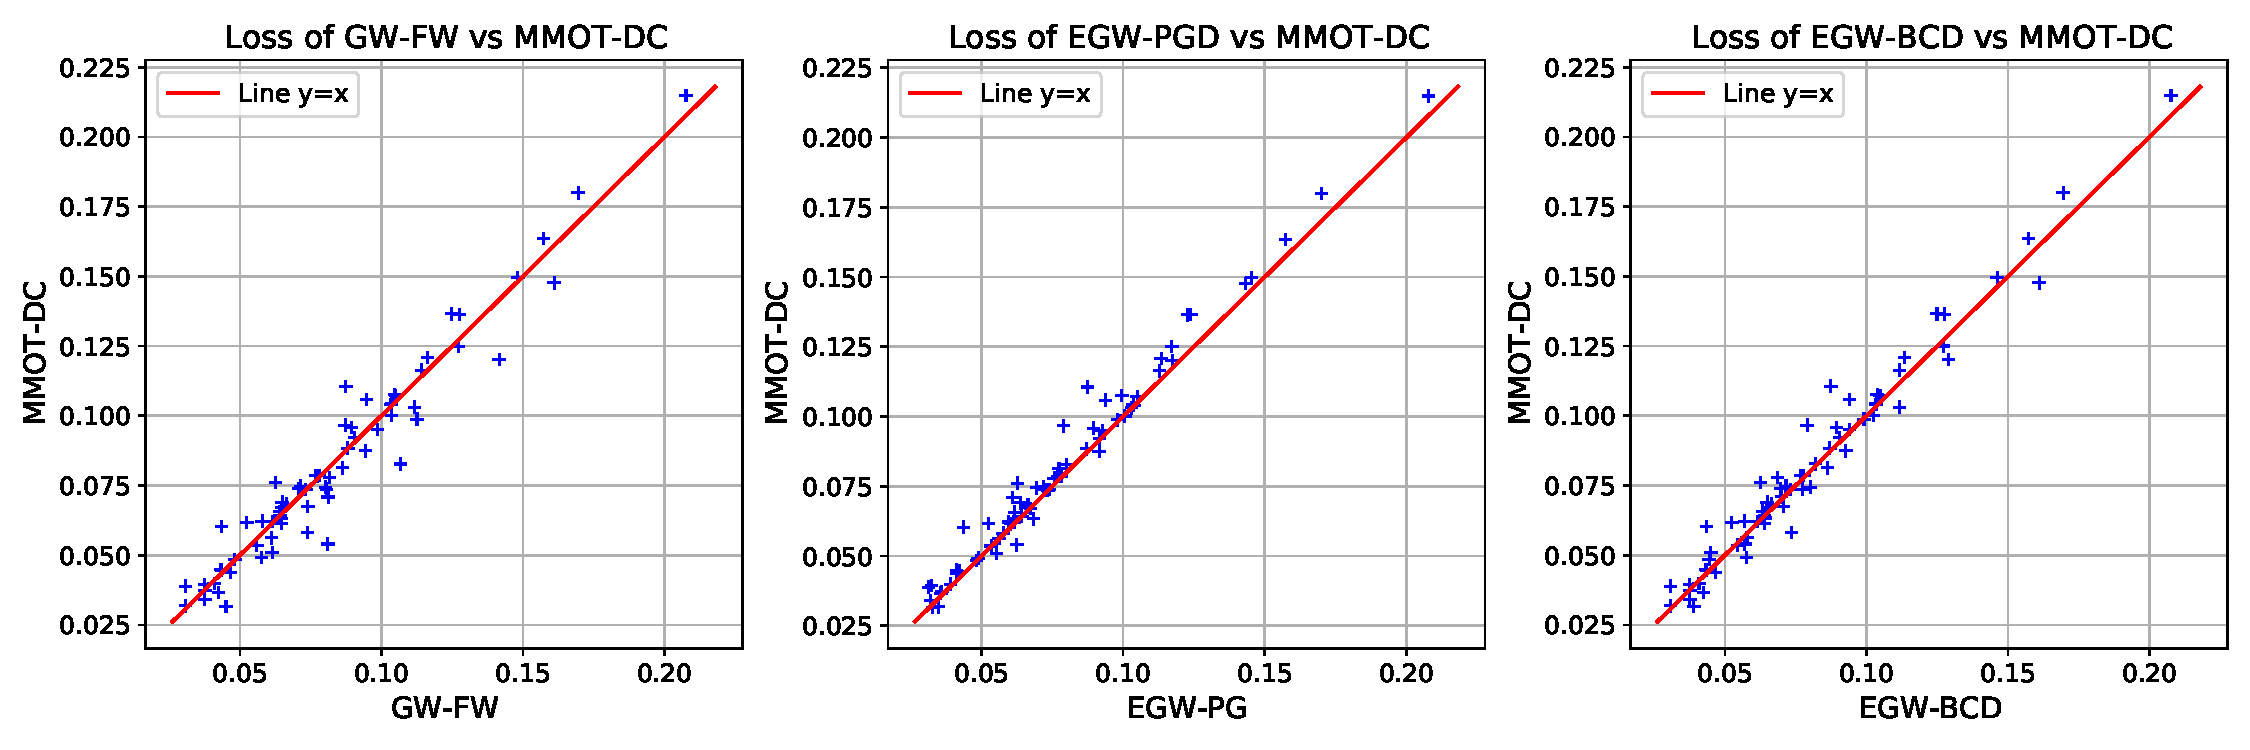
\includegraphics[width=\textwidth,height=\textheight,keepaspectratio]{./Chapitre2/fig/all_vs_MMOT-DC.pdf}
	\caption{Scatter plots of MMOT-DC versus other solvers. In all three plots, the points tend to concentrate around the line $y=x$,
  which indicates the comparable performance of MMOT-DC. On the other hand, the top-right plot shows the clear superiority of EGW-PGD.}
	\label{fig:gw}
\end{figure}
%%%%%%%%%%%%%%%%%%%%%%%%%%%%%%%%%%%%%%%

\paragraph{An empirical variation.} Intuitively, for sufficiently large $\varepsilon$, the minimisation of the KL divergence is prioritised
over the linear term in the objective function of the MMOT-DC problem, which implies that the optimal tensor $P^*$ is "close" to its
corresponding tensor product $P^*_{\# \cT}$. So, instead of calculating the gradient at $P$, one may calculate at
$P_{\# \cT}$. In this case, the gradient reads
\begin{equation}
  \begin{split}
    \sum_{m=1}^M \nabla_P \kl_m(P_{\# \cT}) =
    \log \frac{P_{\# \cT_1}}{\mu^{\otimes}_{\cT_1}} \oplus ... \oplus \log \frac{P_{\# \cT_m}}{\mu^{\otimes}_{\cT_m}} ,
  \end{split}
\end{equation}
where $\oplus$ represents the tensor sum operator between two arbitrary-size tensors: $(A \oplus B)_{i,j}:= A_i + B_j$, where with some
abuse of notation, $i$ or $j$ can be understood as a tuple of indices. Thus, we avoid storing the $N$-D gradient tensor (as in the
\Cref{algo:dc_MMOT}) and only need to store $M$ smaller-size tensors. Not only saving the memory,
this variation also seems to be empirically competitive with the original \Cref{algo:dc_MMOT}, if not sometimes better,
in terms of COOT loss. The underlying reason might be related to the approximate DCA scheme \citep{Thanh15}, where one replaces both
steps in each DC iteration by their approximation. We leave the formal theoretical justification of this variation to the future work.
We call this variation \textit{MMOT-DC-v1} and use the same setup as in Experiment \ref{expe:2}.
\begin{figure}[ht]
  \centering
  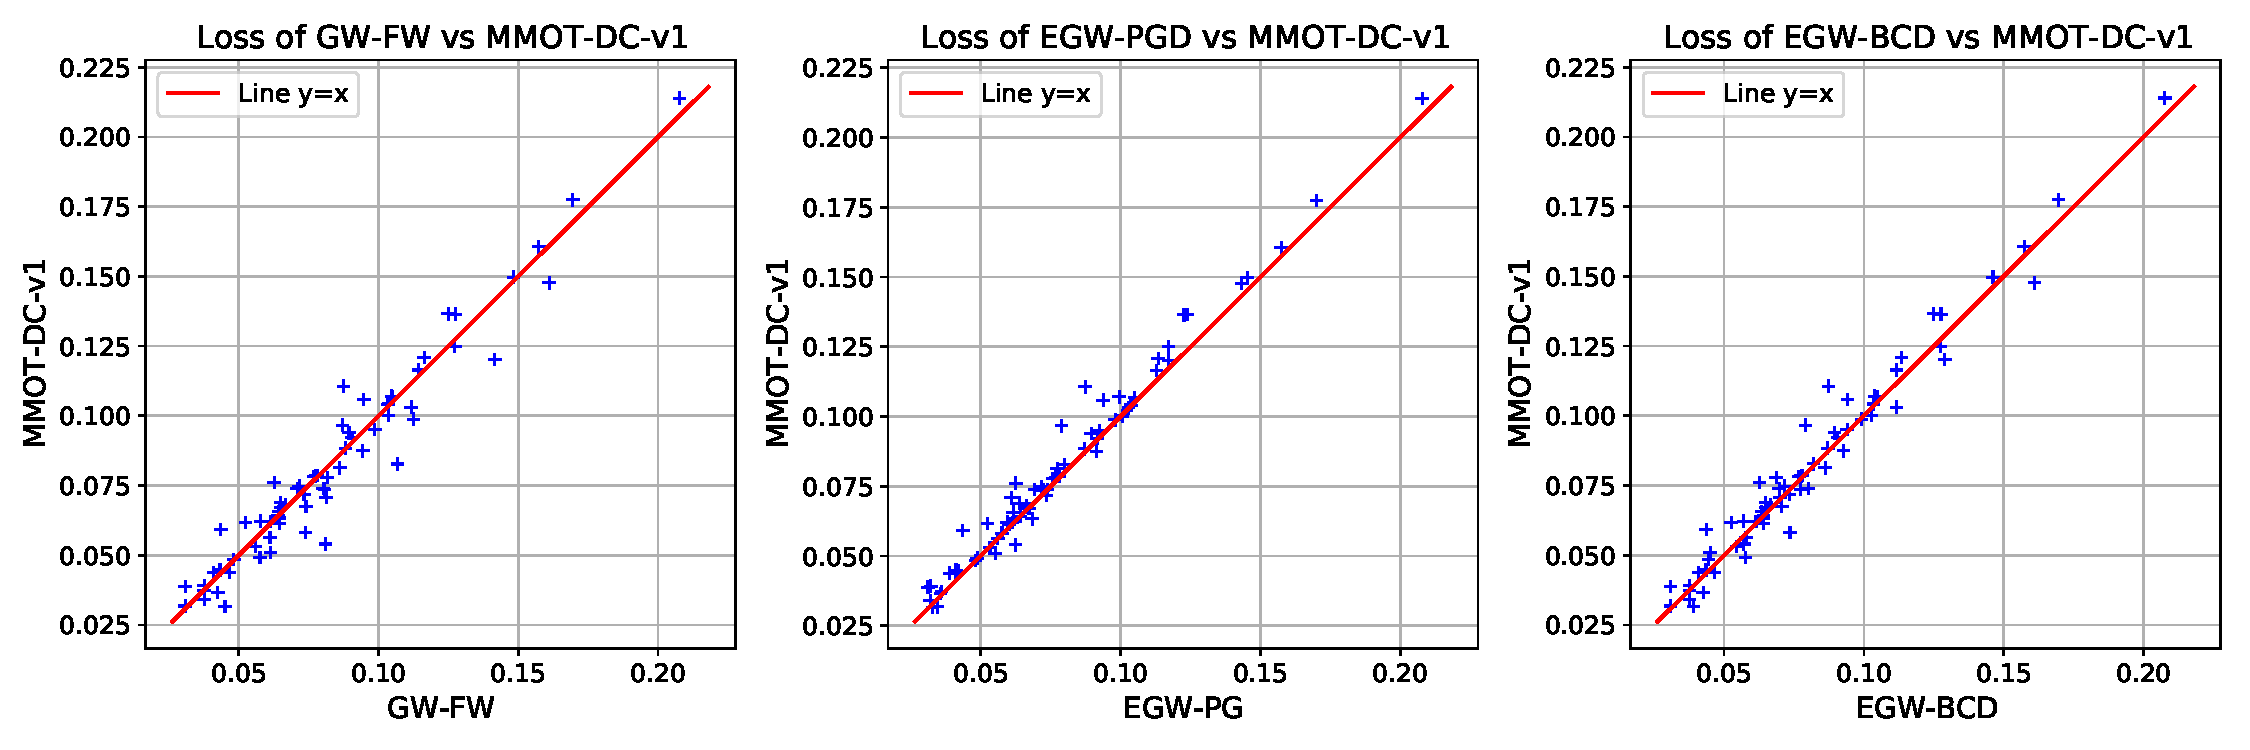
\includegraphics[width=\textwidth,height=\textheight,keepaspectratio]{./Chapitre2/fig/all_vs_MMOT-DC-v1.pdf}
  \caption{Scatter plots of MMOT-DC-v1 versus other solvers. In all three plots, the points tend to concentrate around the line $y=x$,
  which indicates the comparable performance of MMOT-DC-v1. On the other hand, the top-right plot shows the clear superiority of EGW-PGD.}
  \label{fig:coot_mmot_new}
\end{figure}

\begin{table}[H]
  \label{tab:coot_new}
  % \vskip 0.15in
  \begin{center}
    \begin{small}
      \begin{sc}
        \begin{tabular}{|c|c|}
          \hline
          MMOT-DC & MMOT-DC-v1 \\
          \hline
          0.0822 ($\pm$ 0.0364) & 0.0820 ($\pm$ 0.0361) \\
          \hline
        \end{tabular}
      \end{sc}
    \end{small}
  \end{center}
  \caption{Average and standard deviation of COOT loss of MMOT-DC and MMOT-DC-v1.
  The performance of the two algorithms is very similar.}
  % \vskip -0.1in
\end{table}

%%%%%%%%%%%%%%%%%%%%%%%%%%%%%%%%%%%%%%
\subsection{Conclusion and future work}
%%%%%%%%%%%%%%%%%%%%%%%%%%%%%%%%%%%%%%

In this section, we present a novel relaxation of the factorized MMOT problem called \textit{MMOT-DC}.
More precisely, we replace the
hard constraint on factorization constraint by a smooth regularization term. The resulting problem
not only enjoys an interpolation property between MMOT and factorized MMOT, but also is a DC problem,
which can be solved easily by the DC algorithm. We illustrate the use of MMOT-DC the via some simulated experiments and show that
it is competitive with the existing popular solvers of COOT and GW distance.
One limitation of the current DC algorithm is that, it is not scalable because
it requires storing a full-size tensor in the gradient step computation. Thus, future
work may focus on more efficiently designed algorithms, in terms of both time and memory footprint.
Moreover, incorporating additional structure on the cost tensor may also be computationally and practically beneficial.
From a theoretical viewpoint, it is also interesting to study the extension of MMOT-DC to the continuous setting,
which can potentially allow us to further understand the connection between GW distance and COOT.

% From a theoretical viewpoint, one potential application of MMOT-DC is on the study of the sample complexity of GW distance.
% More precisely, given two measure networks $\cX = (X, c_X, \mu_X)$ and $\cY = (Y, c_Y, \mu_Y)$,
% we want to quantify $| \gw(\cX, \cY) - \gw(\cX_n, \cY_n)|$. Note that, \citep{Zhang23} has also
% established the convergence rate for the case of $2$-GW distance, in which the cost function
% is the squared Euclidean distance. Our proposed approach, if works, would be able to handle any
% conditionally negative (or positive) semi-definite kernel.

% The idea is as follows: by \Cref{prop:coot_gw_equiv}, COOT and GW distance are equivalent
% \footnote{Note that one needs to properly extend \Cref{prop:coot_gw_equiv} to the continuous setting
% (of measure networks).}. So, we can replace GW by COOT, as it is less (unnecessarily) constrained.
% Next, we extend MMOT-DC to the continuous setting and show that the interpolation property
% still holds, notably MMOT-DC converges to COOT as regularization tends to the infinity.
% Thanks to the DC algo, we can linearize the MMOT-DC and obtain an entropic MMOT problem.
% This problem has two advantages. First, one can reuse the technique for entropic OT
% in \citep{Genevay19} and extend to the entropic MMOT. Second, for suitable choice of input,
% it approximates COOT.

% Note that, this is still an ongoing work as we have not yet fully resolved all
% technical difficulties. Nevertheless, we report the sketch of the proof and leave most of
% mathematical details in Appendix.

% \paragraph{Assumptions} We assume that the measure networks
% $\cX = (X, c_X, \mu_X)$ and $\cY = (Y, c_Y, \mu_Y)$. $X$ and $Y$ are compact
% subsets of $\bbR^{d_x}$ and $\bbR^{d_y}$, respectively. The probability measures
% $\mu_X$ and $\mu_Y$ are absolutely continuous with respect to the Lebesgue measures
% on $\bbR^{d_x}$ and $\bbR^{d_y}$, respectively.
% With some abuse of notation, we also use $\mu_X, \mu_Y$ to denote their density functions.

% \paragraph{Sketch of proof}
% For convenience, denote $\cU_4 = U(\mu_X, \mu_Y, \mu_X, \mu_Y)$ and $\mu = \mu_X \otimes \mu_Y$.
% We write $c = |c_X - c_Y|^2$ defined by $c(x, y, x', y') = |c_X(x, x') - c_Y(y, y') |^2$.
% Recall that, for any $\pi \in \cU_4$, we denote $\pi_{\#} = \pi_{\# 12} \otimes \pi_{\# 34}$.
% \begin{lemma}
%   For each $\pi \in \cU_4$, denote
%   $G(\pi) := \kl(\pi_{\# 12} | \mu) + \kl(\pi_{\# 34} | \mu) = \kl(\pi_{\#} | \mu^{\otimes 2})$.
%   Then $G$ is convex and differentiable. In particular, $G(\pi) = \int \nabla G(\pi) \; d \pi$,
%   for $\pi \in \cU_4$.
% \end{lemma}
% Now, we have
% \begin{align}
%   \int c \; d\gamma + \varepsilon \kl(\gamma | \gamma_{\#})
%   &\leq \int c \; d\gamma + \varepsilon \kl(\gamma | \mu^{\otimes 2})
%   - \varepsilon \Big[ G(\pi) + \int \nabla G(\pi) \; d \gamma - \int \nabla G(\pi) \; d \pi \Big] \\
%   &= \int \big[ c - \varepsilon \nabla G(\pi) \big] \; d \gamma
%   + \varepsilon \kl(\gamma | \mu^{\otimes 2}).
% \end{align}
% By taking infimum over $\cU_4$, we obtain
% \begin{align}
%   \mmotdc_{\varepsilon} \leq
%   \inf_{\gamma \in \cU_4} \int \big[ c - \varepsilon \nabla G(\pi) \big] d \gamma
%   + \varepsilon \kl(\gamma | \mu^{\otimes 2}).
% \end{align}
% Now, we define the following MMOT problem.
% \begin{definition}
%   For $\pi \in \cU_4$, define
%   \begin{align}
%     \mmot_{\varepsilon}\big( c - \varepsilon \nabla G(\pi) \big) :=
%     \inf_{\gamma \in \cU_4} \int \big[ c - \varepsilon \nabla G(\pi) \big] \; d \gamma
%       + \varepsilon \kl(\gamma | \mu^{\otimes 2}).
%   \end{align}
% \end{definition}
% There exists $\pi \in \cU_4$ such that $\mmot_{\varepsilon}\big( c - \varepsilon \nabla G(\pi) \big)$
% approximates COOT. For example, denote $\pi_{\varepsilon}$
% the solution of the entropic COOT problem $\coot_{\varepsilon}(\cX, \cY)$, we can show that
% \begin{corollary}
%   For every $\varepsilon > 0$, we have
%   $\coot_{1 / \varepsilon}(\cX, \cY) \geq
%   \mmot_{\varepsilon}\big( c - \varepsilon \nabla G(\pi_{1 / \varepsilon}) \big) \geq \mmotdc_{\varepsilon}$.
%   As a consequence,
%   $\mmot_{\varepsilon}\big( c - \varepsilon \nabla G(\pi_{1 / \varepsilon}) \big) \to \coot(\cX, \cY)$,
%   when $\varepsilon \to \infty$.
% \end{corollary}
% Now, suppose $\mmot_{\varepsilon}\big( c - \varepsilon \nabla G(\pi^*) \big)$ can approximate COOT,
% for some $\pi^* \in \cU_4$. Then, by the triangle inequality, we have
% \begin{align}
%   | \coot_(\cX, \cY) - \coot_(\cX_n, \cY_n)|
%   &\leq |\coot_(\cX, \cY) - \mmot_{\varepsilon}\big( c - \varepsilon \nabla G(\pi^*) \big)| \\
%   &+ |\mmot_{\varepsilon, n}\big( c - \varepsilon \nabla G(\pi^*) \big) - \mmot_{\varepsilon}\big( c - \varepsilon \nabla G(\pi^*) \big)| \\
%   &+ |\coot(\cX_n, \cY_n) - \mmot_{\varepsilon, n}\big( c - \varepsilon \nabla G(\pi^*) \big)|,
% \end{align}
% Now, it is enough to bound each term and obtain the final rate. However, the main difficulties
% lie on finding the appropriate choice of $\pi^*$ and on how to control
% it in the entropic MMOT problem.

% \subsection{Stability of Co-Optimal Transport}

% COOT setting: given two sample-feature spaces
% $\cX_1 = ((X_1^s, \mu_1^s), (X_1^f, \mu_1^f), \xi_1)$ and
% $\cX_2 = ((X_2^s, \mu_2^s), (X_2^f, \mu_2^f), \xi_2)$. COOT reads
% \begin{equation}
%     \coot(\cX_1, \cX_2) =
%     \inf_{\substack{\pi^s \in U() \\ \pi^f \in U()}}
%     \int |\xi_1 - \xi_2|^2 d\pi^s d\pi^f
% \end{equation}
% Consider the "semi-empirical" spaces:
% $\widehat{\cX}_i := ((\widehat{X}_i^s, \widehat{\mu}_i^s), (X_i^f, \mu_i^f), \xi_i))$, where
% we fix the dimension $f$ and only consider the empirical version of sample measures.
% Now, how does the feature coupling behave when $\widehat{\mu}^s \to \mu^s$?, i.e. when $n \to \infty$,
% quantify
% \begin{equation}
%     | \coot(\cX_1, \cX_2) -
%     \coot(\widehat{\cX}_1, \widehat{\cX}_2) |
% \end{equation}
% We can first start with finite-dimensional feature spaces (so the feature coupling is a matrix).

\vfill
% }{
% 	% Uncomment this line to compile this chapter locally (when the COMPILE_ALL variable is not set)
% 	%
\chapter[Contributions to CO-Optimal Transport]{Contributions to CO-Optimal Transport}
\label{chap:coot}

\renewcommand{\contentsname}{Contents}
\localtableofcontents*
\chaptermark{\textbf{Contributions to CO-Optimal Transport}}

\hfill \break
This chapter presents two contributions to the CO-Optimal Transport (COOT).
The first one is summarized in \citep{Tran21},
which studies a relaxation of COOT via multi-marginal OT (MMOT).
It unifies several popular OT methods under its umbrella by promoting structural information
on the coupling. We show that incorporating such information into MMOT results in an
instance of a difference of convex (DC) programming problem allowing us to solve it numerically.
Despite high computational cost, the solutions provided by DC optimization are usually
as qualitative as those obtained using available optimization schemes.

The second contribution is on the continuous COOT and its entropic approximation.
We consider a generalization of measure network called \textit{measure hypernetwork}
and show that continuous COOT can be used to compare such objects.
We then study the convergence behavior of the entropic approximation of COOT in the finite-dimensional
setting. Furthermore, under the GW framework, we can quantify the approximation error of
entropic COOT and easily extend this analysis to the GW distance.

\raggedbottom

%%%%%%%%%%%%%%%%%%%%%%%%%%%%%%%%%%%%%%%%%%%%%%%%%%
\section{Background on discrete CO-Optimal Transport}

In many practical applications, the tabular data are usually expressed as a matrix whose rows
represent samples and columns represent features.
In general, the usual OT-based divergences, notably the Wasserstein and GW distances, mostly make
use of the pairwise distances, either within or across domains, to construct the cost matrix
or tensor. This approach has two consequences. First, only sample correspondences are of interest,
By contrast, one completely discards the feature alignments, which can be also interpretable,
for example, in single-cell multi-omics tasks \citep{Demetci20b}.
\footnote{In case of Wasserstein distance, there is no interest of feature correspondences
because intuitively, they are equivalent to the identity matrix. However,
it is no longer clear how to identify the such matching in the GW setting.}.
Second, the distance averages out the features, thus incurs information loss.
This can be problematic in the high-dimensional setting,
where the Euclidean distance is usually not a good metric
(see for example, \citep{Aggarwal01}, or Theorem 3.1.1 and Remark 3.1.2 in \citep{Vershynin18})
\footnote{For more informative discussion,
see \url{https://stats.stackexchange.com/questions/99171/why-is-euclidean-distance-not-a-good-metric-in-high-dimensions}.}.

One way to overcome these limitations is to use the \textit{Co-Optimal Transport} (COOT)
\citep{Redko20}, which learns simultaneously the sample and feature alignments.
In what follows, we denote by $\Delta_{n}= \{p \in \bbR_{> 0}^n: \sum_{i=1}^{n} p_{i}=1\}$
the simplex histogram with $n$ bins. We call $\cX = (X, \mu_1^X, \mu_2^X)$ a \textit{weighted matrix}
defined by a triplet comprised of a matrix $X \in \bbR^{n_x \times d_x}$
equipped with the histograms $\mu_1^X \in \Delta_{n_x}$ and $\mu_2^X \in \Delta_{d_x}$
on its rows and columns, respectively. For $p \geq 1$, we define the COOT between two
weighted matrices $\cX = (X, \mu_1^X, \mu_2^X)$ and $\cY = (Y, \mu_1^Y, \mu_2^Y)$ as
\begin{align}
  \label{eq:discrete_coot}
    \coot(\cX, \cY) :=
    \inf_{\substack{P \in U(\mu_1^X, \mu_1^Y) \\ Q \in U(\mu_2^X, \mu_2^Y)}}
    \sum_{i,j,k,l} (X_{ij} - Y_{kl})^p P_{ik} Q_{jl}.
\end{align}
By Proposition 1 in \citep{Redko20}, if the weights are uniforms,
then COOT defines a distance on the space of weighted matrices,
up to permutation of the matrix coordinates. We note that the formulation \eqref{eq:discrete_coot}
can be easily extended to the multi-coupling setting, for example, in \citep{Kerdoncuff22}.
% They show has shown strong performance of the proposed method in
% heterogeneous domain adaptation.

From the perspective of matrix-comparison, COOT provides a principled way
to compare any two arbitrary-size matrices. By contrast,
this is not the case for many other existing divergences,
whose applicability is summarized in \Cref{t:comparisons}.
\begin{table}[h]
	\centering
		\begin{tabular}{|l|l|l|}
    \hline
    \textbf{Divergences} & \textbf{Input matrices} & \textbf{Requirement on histograms} \\
    \hline
    Matrix norms & Same-size matrices & Not applicable \\
    \hline
    OT, UOT, SW & \makecell[l]{Matrices with the same \\ number of columns}
    & Only requires histogram on rows \\
    \hline
    GW, FGW, UGW, SGW & Square matrices & \makecell[l]{Histograms on rows and columns \\ must be the same} \\
    \hline
    COOT & Arbitrary-size matrices & \makecell[l]{Any histograms on rows and columns} \\
    \hline
		\end{tabular}
		\caption{Applicablility of some popular divergences. COOT is much more flexible than
    other OT-based divergences. UOT and UGW are the unbalaced OT and unbalaced GW divergence, respectively.
    FGW is the Fused GW divergence. SW and SGW denote the sliced Wasserstein \citep{Rabin12,Bonneel15}
    and sliced GW \citep{Vayer19a} distances.
    \label{t:comparisons}}
\end{table}

\paragraph{Co-Optimal Transport as lower bound of GW distance} \label{subsec:GWLB}
Under the framework of discrete GW, where the inputs are similarity matrices, for simplicity,
we write $\cX = (C^x, \mu_X)$, where $C^x$ is the similarity matrix and
$\mu_X$ is the sample histogram. Now, the GW distance can be reformulated as
\begin{align}
  \label{eq:discrete_gw_coot}
  \gw(\cX, \cY) =
  \inf_{\substack{P, Q \in U(\mu_X, \mu_Y) \\ P=Q}}
  \sum_{i,j,k,l} (C^x_{ij} - C^y_{kl})^p P_{ik} Q_{jl},
\end{align}
meaning that we optimize with respect to two independent couplings
under the additional constraint that they must be equal. If it is relaxed, then
one recovers the COOT distance between $\cX$ and $\cY$. We also stress that COOT should not
be confused with the third lower bound of the GW distance \citep{Memoli07,Memoli11} defined as
\begin{equation}
  \text{TLB}(\cX, \cY) :=
  \inf_{Q \in U(\mu_X, \mu_Y)}
  \Big( \inf_{P \in U(\mu_X, \mu_Y)} \sum_{i,j,k,l} (C^x_{ij} - C^y_{kl})^p P_{ik} \Big) Q_{jl}.
\end{equation}
In particular, we have $\gw(\cX, \cY) \geq \coot(\cX, \cY) \geq \text{TLB}(\cX, \cY)$.

% The equivalence between BAP and QAP has already been studied in \citep{Konno76}.
If the inputs are the Euclidean, or squared Euclidean distances, then equality holds between
COOT and GW distances \citep{Sejourne20,Redko20}. These results are based on the prior works
of \citet{Konno76,Maron18} and summarized in the folllowing proposition.
\begin{definition}
  A square matrix $A \in \bbR^{n \times n}$ is conditionally negative semi-definite (CND)
  if it is symmetric and for any $c \in \bbR^n$ such that $\sum_i c_i = 0$, we have
  $c^T A c \leq 0$.
\end{definition}
%%%%%%%%%%%%%%%%%%%%%%%%%%%%%%%%%%%%%%%%%%%%%%%%%%%%%%%%
\begin{proposition}
  \label{prop:coot_gw_equiv}
  For $p=2$, suppose that $C^x$ and $C^y$ are of the forms:
  $C^x_{ij} = f_i + f_j + A_{ij}$ and $C^y_{kl} = g_k + g_l + B_{kl}$,
  where $f, g$ are vectors in $\bbR^m, \bbR^n$, respectively,
  and the matrices $A, B$ are CND. Then $\gw(\cX, \cY) = \coot(\cX, \cY)$.
  Furthermore, if $(P_1^*, P_2^*)$ is a solution of the COOT problem, then $P_1^*$ and $P_2^*$
  are two solutions of the GW problem. In particular,
  if the semi-definiteness is replaced by the definiteness, then $P_1^* = P_2^*$.
\end{proposition}
In particular, if the similarity matrices is CND,
then one can safely remove the equality constraint without changing the minimum.
Thus, \Cref{prop:coot_gw_equiv} justifies the rationale behind
the alternative minimization procedure for GW distance presented in \Cref{subsec:gw_approx}.
This scheme is easily adapted to the entropic fused GW problem, by observing that,
for any reference histogram $\mu \in \bbR_{> 0}^{m \times n}$, we have
\begin{equation}
  \begin{split}
    &\inf_{\substack{P \in U(\mu_X, \mu_Y)}}
  \sum_{i,j,k,l} (C^x_{ij} - C^y_{kl})^p P_{ik} P_{jl}
  + \alpha \langle D, P \rangle + \varepsilon \; \kl(P | \mu) \\
  &= \inf_{\substack{P \in U(\mu_X, \mu_Y) \\ Q \in U(\mu_X, \mu_Y) \\ P = Q }}
  \sum_{i,j,k,l} (C^x_{ij} - C^y_{kl})^p P_{ik} Q_{jl}
  + \frac{\alpha}{2} \langle D, P \rangle + \frac{\alpha}{2} \langle D, Q \rangle
  + \frac{\varepsilon}{2} \kl(P | \mu) + \frac{\varepsilon}{2} \kl(Q | \mu).
  \end{split}
\end{equation}
Again, under exactly the same conditions on the similarity matrices in \Cref{prop:coot_gw_equiv},
one can safely drop the equality constraint during the optimization.

%%%%%%%%%%%%%%%%%%%%%%%%%%%%%%%%%%%%%%
\section{Continuous Co-Optimal Transport}
%%%%%%%%%%%%%%%%%%%%%%%%%%%%%%%%%%%%%%

In this section, we present our unpublished work on the continuous COOT and its entropic approximation.
We will mostly follow the terminology and concepts proposed in \citep{Chowdhury21b}.

\subsection{Formulation and preliminary results}

As already seen in discrete GW problem \eqref{eq:discrete_gw_coot},
by rewriting a measure network $\cX = (X, c_X, \mu_X)$ as
$\widetilde{\cX} = \big((X_1, \mu_1^X), (X_2, \mu_2^X), c_X \big)$, with
$X_1 = X_2 = X$ and $\mu_1^X = \mu^X_2 = \mu_X$, one can reformulate the GW problem as
\begin{equation}
  \begin{split}
    \inf_{\pi_1, \pi_2}
    &\int_{X_1 \times Y_1} \int_{X_2 \times Y_2}
    \big\vert c_X(x_1, x_2) - c_Y(y_1, y_2) \big\vert^p \; d\pi_1(x_1, y_1) \; d\pi_2(x_2, y_2). \\
    \text{ subject to: } &\pi_k \in U(\mu_k^X, \mu_k^Y), \forall k = 1,2, \\
    &\pi_1 = \pi_2.
  \end{split}
\end{equation}
When the equality constraint on the two couplings is relaxed,
we can allow that either $X_1 \neq X_2$ or $Y_1 \neq Y_2$.
The interest of such situation can be found, for example, in heterogenous domain adaptation,
where $X_1$ and $Y_1$ represent the "sample" spaces in the source and target domains, respectively,
and $X_2$ and $Y_2$ represent the "feature" spaces in the source and target domains, respectively.
As a result, the corresponding "sample" and "feature" couplings are also different in their natures.

% Before defining the continuous extension of COOT, we need to specify the
% To this extent, we need to extend the prior work of \citep{Chowdhury19} on measure network.

\begin{definition}[Measure hypernetwork \citep{Chowdhury21b}]
Suppose $(X_1, \mu_1^X)$ and $(X_2, \mu_2^X)$ are two Polish measure spaces,
and $c_X$ is a bounded measurable function on $X_1 \times X_2$.
We call the triplet $\cX = \big((X_1, \mu_1^X), (X_2, \mu_2^X), c_X \big)$
a \textbf{measure hypernetwork}. We also say $c_X$ is the \textbf{interaction}
between $X_1$ and $X_2$.
\end{definition}
Without risk of confusion, when $X_1 = X_2 = X$ and $\mu_1^X = \mu_2^X = \mu_X$,
we use interchangeably "measure hypernetwork" and "measure network" in
the context of GW \citep{Chowdhury19}.
When $X_1$ and $X_2$ are finite spaces (so $\mu_1^X$ and $\mu_2^X$ are histograms),
we call $\cX$ a finite measure hypernetwork. For convenience, we also refer the index $1$ as "sample"
and $2$ as "feature", for example, $X_1$ is the sample space, $\pi_2$ is the feature coupling.
\begin{definition}[COOT distance between measure hypernetworks \citep{Chowdhury21b}]
  \label{def:cont_coot}
  For $p \geq 1$, the COOT distance between two measure hypernetworks $\cX$ and $\cY$ is defined as
  \begin{align} \label{eq:cont_coot}
    \coot(\cX, \cY) =
    \inf_{\substack{\pi_1 \in U(\mu^X_1, \mu^Y_1) \\
    \pi_2 \in U(\mu^X_2, \mu^Y_2)}} \iint
    \big\vert c_X(x_1, x_2) - c_Y(y_1, y_2) \big\vert^p \; d\pi_1(x_1, y_1) \; d\pi_2(x_2, y_2).
  \end{align}
\end{definition}
It is not difficult to see that \Cref{def:cont_coot} generalizes the discrete COOT \citep{Redko20}.
In practice, the input data is usually expressed as matrix,
whose rows represent samples and columns represent features.
In this case, the interaction value is precisely the coordinate of the data matrix.
Meanwhile, the sample and feature spaces are unknown and have little interest and importance.

% \begin{figure}[ht]
%   \centering
%   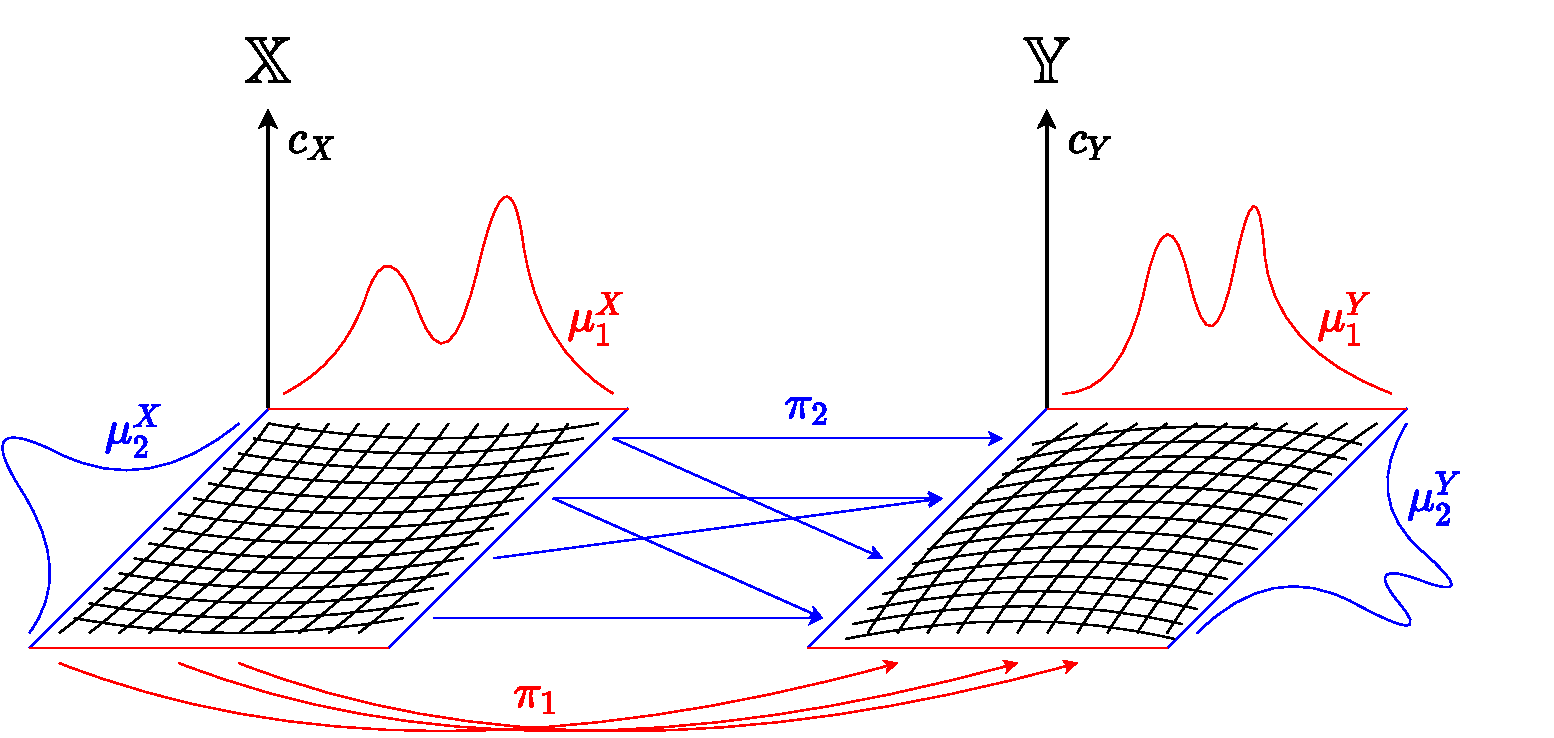
\includegraphics[width=0.9\textwidth, keepaspectratio]{./Chapitre2/fig/coot_diagram.pdf}
%   \caption{Scatter plots of MMOT-DC-v1 versus other solvers. In all three plots, the points tend to concentrate around the line $y=x$,
%   which indicates the comparable performance of MMOT-DC-v1. On the other hand, the top-right plot shows the clear superiority of EGW-PGD.}
%   \label{fig:continuous_coot}
% \end{figure}
First, we can show that the COOT problem \eqref{eq:cont_coot} is well defined.
\begin{proposition}[Lemma 35 in \citep{Chowdhury21b}]
  \label{prop:exist_coot}
  The COOT problem always admits a minimizer.
\end{proposition}
We provide the proof in Appendix \ref{annex:cont_coot}.
While the proofs of our result and of Lemma 35 in \citep{Chowdhury21b} use the same proof technique of
Theorem 2.2 in \citep{Chowdhury19}, ours is slightly different. More precisely,
we exploit a different reformulation of COOT, where it can be rewritten as a multi-marginal OT problem
with additional factorization constraint on the coupling. Later, we will see that,
this observation also allows to establish the convergence result of entropic COOT.

%%%%%%%%%%%%%%%%%%%%%%%%%%%%%%%%%%%%%%%%%%
\subsection{Metric properties}

The framework on the GW isomorphism presented in \Cref{subsec:prop_gw}
can be extended immediately to the COOT setting. In particular, while our
presentation is different to that of \citep{Chowdhury21b}, we still come up with the
same metric properties.

%%%%%%%%%%%%%%%%%%%%%%%%%%%%%%%%%%%%%%%%%
\begin{definition}[Relaxed mass splitting]
  A measure hypernetwork $\cZ$ is a \textbf{relaxed mass splitting} (RMS) of a
  measure hypernetwork $\cX$ if there exist two measure-preserving maps
  $\varphi_k: Z_k \to X_k$, for $k=1,2$, such that the pullback equality
  $c_Z = (\varphi_1, \varphi_2)^*c_X$ holds $\mu^Z_1 \otimes \mu_2^Z$-almost everywhere
  in $Z_1 \times Z_2$. We denote $\ms(\cX)$ the set of all mass splittings
  of $\cX$. This pair of maps $(\varphi_1, \varphi_2)$ is also called
  \textbf{basic weak isomorphism} in \citep{Chowdhury21b}.
\end{definition}
We denote $\rms(\cX)$ the set of all relaxed mass splittings of $\cX$. Clearly,
$\cX \in \rms(\cX)$, so $\rms(\cX)$ is not empty.
In particular, for measure networks, if $\cZ \in \ms(\cX)$, then $\cZ \in \rms(\cX)$,
meaning that $\ms(\cX) \subset \rms(\cX)$. Now, we can define the isomorphism between
the measure hypernetworks as follows.
\begin{definition}[COOT-isomorphism] \label{coot_isomorphic}
  Two measure hypernetworks are
  \begin{enumerate}
    \item strongly isomorphic if there exist two \textbf{bijective}
    measure-preserving map from one hypernetwork to the other such that the pullback equality holds
    \textbf{everywhere}.
    \item semi-strongly isomorphic if one is the RMS of the other and vice versa.
    \item weakly isomorphic if they have a common RMS.
  \end{enumerate}
\end{definition}
This is an immediate relaxation of the GW isomorphism. In particular,
in case of measure networks, isomorphism in GW sense implies COOT isormorphism.
The following result summarizes the relations amongst the three types of COOT isomorphism.
%%%%%%%%%%%%%%%%%%%%%%%%%%%%%%%%%%%%%%%%%%%%%%%%
\begin{corollary} \label{prop:strong_weak_iso}
  Given two measure hypernetworks $\cX$ and $\cY$. Consider three statements
  \begin{enumerate}
    \item[(1)] $\cX$ and $\cY$ are strongly isomorphism.
    \item[(2)] $\cX$ and $\cY$ are semi-strongly isomorphism.
    \item[(3)] $\cX$ and $\cY$ are weakly isomorphism.
  \end{enumerate}
  Then, the following relations hold
  \begin{enumerate}
    \item $(1) \implies (2) \implies (3)$.
    \item If $\cX$ and $\cY$ are finite, then $(2) \implies (1)$.
    \item If $\cX$ and $\cY$ are finite such that $|X_k| = |Y_k|$
    and $\mu_k^X, \mu_k^Y$ are uniform distributions, for $k = 1,2$, then
    $(3) \implies (2)$. This means all three forms are equivalent.
  \end{enumerate}
\end{corollary}
%%%%%%%%%%%%%%%%%%%%%%%%%%%%%%%%%%%%%%%%%%%%%%%%
Now, we can characterize the weak isomorphism by
\begin{proposition} \label{prop:coot_iso}
  Two measure hypernetworks $\cX$ and $\cY$ are COOT-weakly isomorphic if and only if
  $\coot(\cX, \cY) = 0$.
\end{proposition}
%%%%%%%%%%%%%%%%%%%%%%%%%%%%%%%%%%%%%%%%%%%%%%%%
\begin{proposition}[Theorem 1 in \citep{Chowdhury21b}] \label{prop:metric_prop}
  $\coot^{1/p}$ defines a metric on the space of measure hypernetworks, up to COOT-weak isomorphism.
\end{proposition}
%%%%%%%%%%%%%%%%%%%%%%%%%%%%%%%%%%%%%%%%%
% \paragraph{Discussion on the setting of mm-space}
% While the measure network can fit in the COOT framework, this is usually not the case for
% the mm-space since the distance function is only measurable in Polish space,
% but not necessarily bounded. However, all previous results on the existence of minimizer and
% metric property remain unchanged if one replaces measure hypernetworks by mm-spaces,
% as long as COOT is finite. Moreover,
% \begin{corollary}
% For $p=2$, all forms of COOT isomorphisms are equivalent and
% they are also equivalent to the isomorphism in GW sense.
% \end{corollary}
% This indicates that, both GW distance and COOT can be used to compare isometric objects,
% namely those transformed by reflection, rotation or translation.

%%%%%%%%%%%%%%%%%%%%%%%%%%%%%%%%%%%%%%%%%%%%%%%%
\subsection{Entropic regularization and approximation error}
%%%%%%%%%%%%%%%%%%%%%%%%%%%%%%%%%%%%%%%%%%%%%%%%
Similar to the Wasserstein and GW distances, one can approximate the COOT with entropic regularization.
In this thesis, we are interested in the following formulation of entropic COOT:
for $\varepsilon > 0$,
\begin{align}
  \coot_{\varepsilon} (\cX, \cY) =
  \inf_{\substack{\pi_1 \in U(\mu^X_1, \mu^Y_1) \\
  \pi_2 \in U(\mu^X_2, \mu^Y_2)}} &\iint
  \big\vert c_X(x_1, x_2) - c_Y(y_1, y_2) \big\vert^p \; d\pi_1(x_1, y_1) \; d\pi_2(x_2, y_2) \\
  &+ \varepsilon \; \kl \big( \pi_1 \otimes \pi_2 \vert (\mu^X_1 \otimes \mu^Y_1) \otimes (\mu^X_2 \otimes \mu^Y_2) \big).
\end{align}
Note that, this structure of the KL divergence term is particularly handy to prove all results related to
the entropic COOT. It also bears similarity with the \textit{quadratic divergence}
\citep{Sejourne20} defined by $\kl^{\otimes 2}(\mu, \nu):= \kl(\mu \otimes \mu | \nu \otimes \nu)$,
which is used to define the unbalanced GW divergence. Note that, in the balanced setting,
the joint penalization in terms of KL divergence is in fact equivalent to the
independent KL-penalization. More precisely, given any $\pi_k \in U(\mu_k^X, \mu_k^Y)$,
for $k=1,2$, we have
\begin{equation}
  \kl \big( \pi_1 \otimes \pi_2 \vert (\mu^X_1 \otimes \mu^Y_1) \otimes (\mu^X_2 \otimes \mu^Y_2) \big)
  = \kl(\pi_1 \vert \mu^X_1 \otimes \mu^Y_1) + \kl(\pi_2 \vert \mu^X_2 \otimes \mu^Y_2).
\end{equation}
In practice, since the couplings may not have the same nature (for example,
when working directly with the input data, rather than via the similarity matrix),
they can be penalized by different values of regularization.
%%%%%%%%%%%%%%%%%%%%%%%
\begin{proposition}
The entropic COOT problem always admits a minimizer.
\end{proposition}
%%%%%%%%%%%%%%%%%%%%%%%
One major practical interest of entropic COOT is that, for sufficiently small regularization,
it provides a good proxy for unregularized COOT. To formalize this observation, first,
we need to introduce the following assumption on the measure hypernetwork.
%%%%%%%%%%%%%%%%%%%%%%%%%%%%%
\begin{assumption}
  \label{assump:ent_coot}
  Given a measure hypernetwork, we assume that
  \begin{enumerate}
    \item[A1] The sample and feature spaces are finite-dimensional vector spaces.
    \item[A2] Their associated Borel probability measures are absolutely continuous
    with respect to the Lebesgue measure.
  \end{enumerate}
\end{assumption}
%%%%%%%%%%%%%%%%%%%%%%%%%%%%%%
\begin{proposition} \label{prop:conv_ent_coot}
  Under \Cref{assump:ent_coot}, if the interactions are continuous, then
  $\coot_{\varepsilon}(\cX, \cY) \to \coot(\cX, \cY)$ when $\varepsilon \to 0$. Moreover,
  let $(\varepsilon_n)_{n \in \bbN}$ be a sequence of
  positive regularizations such that $\varepsilon_n \to 0$.
  Denote $\pi_n := (\pi_{1, n}, \pi_{2, n})$ the solution of the entropic problem
  $\coot_{\varepsilon_n} (\cX, \cY)$. Then, any cluster point of the sequence $(\pi_n)_n$ is
  a solution of the unregularized COOT problem.
\end{proposition}
%%%%%%%%%%%%%%%%%%%%%%%%%%%%%%
The above result is similar to the one known in entropic OT \citep{Carlier17}. This is due to the fact
that the entropic COOT can be reformulated as a variant of multi-marginal OT problem,
thus the block approximation and $\Gamma$-convergence techniques can be applied.

Furthermore, still under \Cref{assump:ent_coot}, if the measure network is bounded,
then we can quantify the approximation error as follows.
%%%%%%%%%%%%%%%%%%%%%%%%%%%%%%
\begin{proposition} \label{prop:quant_bound_ent}
  Given two measure networks $\cX = (X, \mu_X, c_X)$ and $\cY = (Y, \mu_Y, c_Y)$.
  Suppose that $X$ is bounded subset of $\bbR^{d_x}$ and $Y$ is a bounded subset
  of $\bbR^{d_y}$, where $\diam(X), \diam(Y) \leq D$.
  Denote $d = \max(d_x, d_y)$. Suppose there exists a constants $q > 0$ such that
  $c_X(x_1, x_2) = \vert\vert x_1 - x_2 \vert\vert^q$, for every $(x_1,x_2) \in X^2$, and
  $c_Y(y_1, y_2) = \vert\vert y_1 - y_2 \vert\vert^q$, for every $(y_1,y_2) \in Y^2$. Then,
  \begin{equation}
    \coot_{\varepsilon}(\cX, \cY) - \coot(\cX, \cY) \leq
    \frac{2d \varepsilon}{pq} \log\Big( \frac{pq (2D d^{1/p})^{pq}}{2d \varepsilon} \Big).
  \end{equation}
\end{proposition}
%%%%%%%%%%%%%%%%%%%%%%%%%
This bound is very similar to the one in Wasserstein setting \citep{Genevay19}.
Let us consider two special cases of \Cref{prop:quant_bound_ent}.
\begin{itemize}
  \item[$\bullet$] When $p=2$ and $c_X, c_Y$ are Euclidean distances (\ie, $q=1$),
  the upper bound becomes $d\varepsilon \log\Big( \frac{4D^2}{\varepsilon} \Big)$.

  \item[$\bullet$] When $p=2$ and $c_X, c_Y$ are squared Euclidean distances
  (\ie, $q=2$), the upper bound becomes
  $\frac{d\varepsilon}{2} \log\Big( \frac{32dD^4}{\varepsilon} \Big)$.
\end{itemize}
In both situations, the dependence of the bound on the maximal distance $D$ between points
within each space (even only at logarithmic scale) and on the dimension $d$ indicates
that either high dimensional space, or large intra-space distance (for example, due to outliers)
can have negative impact on the approximation error. On the other hand,
by comparing these two bounds, we deduce that if $\log(2d \varepsilon) \leq 1$,
then the squared Euclidean distances generates a provably better (smaller) upper bound.

With little modification of the proof, exactly the same upper bound in \Cref{prop:quant_bound_ent}
holds for GW distance. We note that \citet{Zhang23} also establish a similar
$O(\varepsilon \log \varepsilon)$-approximation error between the unregularized and entropic GW,
but they rely on different assumptions to ours. In particular, their result only holds
for $2$-GW distance, when the distance function is the squared-Euclidean norm. By contrast,
\Cref{prop:quant_bound_ent} holds for any $p$-GW distance and any $L^q$-norm as distance function.

%%%%%%%%%%%%%%%%%%%%%%%%%%%%%%%%%%%%%%
\section{Factored couplings in Multi-marginal Optimal
Transport via Difference of Convex programming} \label{subsec:MMOT_DC}

%%%%%%%%%%%%%%%%%%%%%%%%%%%%%%%%%%%%%%%
\subsection{Introduction}

Broadly speaking, the classic OT problem provides a principled approach for transporting one probability distribution onto another
following the principle of the least effort. Such a problem, and the distance on the space of probability distributions derived from it,
arise in many areas of machine learning (ML) including generative modeling, transfer learning and information retrieval, where OT has
been successfully applied. A natural extension of classic OT, in which the admissible transport plan can have more
than two prescribed marginal distributions, is called the multi-marginal optimal transport (MMOT) \citep{Gangbo98}.
The latter has several attractive properties: it enjoys a duality theory \citep{Kellerer84} and finds connections with the
probabilistic graphical models \citep{Haasler20} and the Wasserstein barycenter problem \citep{Agueh11} used for data averaging.
While being less popular than the classic OT with two marginals, MMOT is a very useful framework on its own with some notable recent
applications in generative adversarial networks \citep{Cao19}, clustering \citep{Mi21} and domain adaptation
\citep{HuiLCHY18,HeZKSC19}, to name a few.

The recent success of OT in ML is often attributed to the entropic regularization \citep{Cuturi13} where the authors imposed a
constraint on the coupling matrix forcing it to be closer to the independent coupling given by the rank-one product of the marginals.
Such a constraint leads to the appearance of the strongly convex entropy term in the objective function and allows the entropic
OT problem to be solved efficiently using simple Sinkhorn-Knopp matrix balancing algorithm. In addition to this, it was also noticed
that structural constraints on the coupling and cost matrices allow to reduce the high computational cost and sample complexity
of the classic OT problem \citep{Genevay19,Forrow18,Chiheng21,Meyer21a}. However, none of these works considered a much more
challenging case of doing so in a multi-marginal setting. On the other hand, while the work of \citet{Haasler20} considers the MMOT
problem in which the cost tensor induced by a graphical structure, it does not naturally promote the factorizability of
transportation plans.

\paragraph{Contributions} In this work, we define and study a general MMOT problem with structural penalization on the coupling matrix.
We start by showing that a such formulation includes several popular OT methods as special cases and allows to gain deeper insights
into them. We further consider a relaxed problem where the hard constraint is replaced by a regularization term and show that it leads
to an instance of the difference of convex programming problem. A numerical study of the solutions obtained when solving the latter
in cases of interest highlights their competitive performance when compared to solutions provided by the optimization
strategies used previously.

%%%%%%%%%%%%%%%%%%%%%%%%%%%%%%%%%%%%%
\subsection{Preliminary knowledge}

\paragraph{Notations.} For each integer $n \geq 1$, we write $[n] := \{1,...,n\}$.
We denote $\langle \cdot, \cdot \rangle$ denotes the Frobenius inner product.
The generalized Kullback-Leibler divergence between two positive vectors $p, q \in \bbR^n_{> 0}$
is defined as $\kl(p | q) = \sum_i p_i \log \frac{p_i}{q_i} - \sum_i p_i + \sum_i q_i$,
with the convention that $0 \log 0 = 0$.

In what follows, given an integer $N \geq 1$, for any positive integers $a_1,..., a_N$, we call
$P \in \bbR^{a_1 \times ... \times a_N}$ a $N$-D tensor. In particular, a $1$-D tensor is a vector and $2$-D tensor is a matrix.
A tensor is a probability tensor if its entries are nonnegative and the sum of all entries is $1$.
Given $N$ probability vectors $\mu_1, ..., \mu_N$, we write $\mu = (\mu_n)_{n=1}^N$
and $\mu^{\otimes} := \mu_1 \otimes ... \otimes \mu_N$.
We denote $\Sigma$ the set of $N$-D probability tensors and $U(\mu) \subset \Sigma$ the set of nonnegative tensors whose $N$
marginal distributions are $\mu_1, ..., \mu_N$. In this case, any coupling in $U(\mu)$ is said to be \textit{admissible}.

\paragraph{Multi-marginal OT problem.} Given a collection of $N$ probability vectors $\mu = (\mu_n \in \bbR^{a_n})_{n=1}^N$
and a $N$-D cost tensor $C \in \bbR^{a_1 \times ... \times a_N}$, the MMOT problem reads
\begin{equation*}
  \mmot(\mu) = \inf_{P \in U(\mu)} \langle C, P \rangle.
\end{equation*}
In practice, such a formulation is intractable to optimize in a discrete setting as it results in a linear program where the number
of constraints grows exponentially in $N$. A more tractable strategy for solving MMOT is to consider the following entropic
regularization problem
\begin{equation} \label{MMOT_primal}
  \inf_{P \in U(\mu)} \langle C, P \rangle + \varepsilon \kl(P | \mu^{\otimes}).
\end{equation}
which can be solved using Sinkhorn's algorithm \citep{Benamou14}.
We refer the interested reader to Appendix \ref{appendix:subsec_mmot_dc} for algorithmic details.

%%%%%%%%%%%%%%%%%%%%%%%%%%%%%%%%%%%%%%%%%%%%%%%%%
\subsection{Factored Multi-marginal Optimal Transport}

In this section, we first define a factored MMOT (F-MMOT) problem where we seek to promote a structure on the optimal coupling
given such as a factorization into a tensor product. Interestingly, such a formulation can be shown to include several other
OT problems as special cases. Then, we introduce a relaxed version called MMOT-DC where the factorization constraint is
smoothly promoted through a Kullback-Leibler penalty.

\subsubsection{Motivation}

Before a formal statement of our problem, we first give a couple of motivating examples showing
why and when structural constraints on the coupling matrix can be beneficial. To this end,
first note that a trivial example of the usefulness of such constraints in OT is the famous
entropic regularization. Indeed, while most of the works define the latter by adding
negative entropy of the coupling to the classic OT objective function directly,
the original idea was to constraint the sought coupling to remain close (to some extent)
to a rank-one product of the two marginal distributions. The appearance of negative entropy
in the final objective function is then only a byproduct of such constraint due to
the decomposition of the KL divergence into a sum of three terms with two of them being constant.
Below we give two more examples of real-world applications related to MMOT problem
where a certain decomposition imposed on the coupling tensor can be desirable.
\paragraph{Multi-source multi-target translation.} A popular task in computer vision is
to match images across different domains in order to perform the so-called image translation.
Such tasks are often tackled within the GAN framework where one source domain from which
the translation is performed, is matched with multiple target domains modeled using generators.
While MMOT was applied in this context by \citet{Cao19} when only one source was considered,
its application in a multi-source setting may benefit from structural constraints
on the coupling tensor incorporating the human prior on what target domains each source domain
should be matched to.

\paragraph{Multi-task reinforcement learning.} In this application, the goal is to learn
individual policies for a set of agents while taking into account the similarities between them
and hoping that the latter will improve the individual policies. A common approach is
to consider an objective function consisting of two terms where the first term is concerned
with learning individual policies, while the second forces a consensus between them.
Similar to the example considered above, MMOT problem was used to promote the consensus
across different agents' policies in \citep{Cohen21}, even though such a consensus
could have benefited from a prior regarding the semantic relationships between the learned tasks.
%
%We can cite other examples motivating the introduction of structural constraints in MMOT problem but the bottom line of it remains unchanged: imposing a certain structure on the optimal coupling tensor is a way of incorporating the human-based priors to the MMOT problem that reflect the domain knowledge about the problem at hand. We now proceed to the formal introduction of this idea.

\subsubsection{Factored MMOT and its relaxation}
We start by giving several definitions used in the following parts of this section.
%We call $P \in \bbR^{a_1 \times ... \times a_N}$ a $N$-D tensor. When $N=1$, we simply call it a vector and when $N=2$,
%it is a matrix.
\begin{definition}[Tuple partition]
 Given two integers $N \geq M \geq 2$, a sequence of tuples $\cT = (\cT_m)_{m=1}^M$, is called a
 \underline{tuple partition} of the $N$-tuple $(1,...,N)$ if the tuples $\cT_1, ..., \cT_M$ are nonempty and disjoint,
 and their concatenation in this order gives $(1,...,N)$.
\end{definition}
Here, we implicitly take into account the order of the tuple, which is not the case for the partition of the set $[N]$. If
there exists a tuple in $\cT$ which contains only one element, then we say $\cT$ is \textit{degenerate}.

\begin{definition}[Marginal tensor]
  Given a tensor $P \in \bbR^{a_1 \times ... \times a_N}$ and a tuple partition $\cT = (\cT_m)_{m=1}^M$,
  we call $P_{\# \cT_m}$ its \underline{$\cT_m$-marginal tensor}, by summing $P$ over all dimensions not in $\cT_m$.
  We write $P_{\# \cT} = P_{\# \cT_1} \otimes ... \otimes P_{\# \cT_M} \in \bbR^{a_1 \times ... \times a_N}$
  the tensor product of its marginal tensors.
\end{definition}
For example, for $M=N=2$, we have $\cT_1 = (1)$ and $\cT_2 = (2)$. So, given a matrix
$P \in \bbR^{a_1 \times a_2}$, its marginal tensors $P_{\# \cT_1}$ and $P_{\# \cT_2}$ are simply vectors in
$\bbR^{a_1}$ and $\bbR^{a_2}$, respectively, defined by $(P_{\# \cT_1})_i = \sum_j P_{ij}$ and
$(P_{\# \cT_2})_j = \sum_i P_{ij}$ for $(i,j) \in [a_1] \times [a_2]$. The tensor product
$P_{\# \cT} \in \bbR^{a_1 \times a_2}$ is then defined by
$(P_{\#\cT})_{ij} = (P_{\# \cT_1})_i (P_{\# \cT_2})_j$.
Clearly, if $P$ is a probability tensor, then so are its marginal tensors and tensor product.

Suppose $\cT_m = (p,...,q)$ for some $m \in [M]$ and $1 \leq p \leq q \leq N$. We denote
$\Sigma_{\cT_m}$ the set of probability tensors in $\bbR^{a_p \times ... \times a_q}$ and
$U_{\cT_m} \subset \Sigma_{\cT_m}$ the set
of probability tensors in $\bbR^{a_p \times ... \times a_q}$ whose
$r^{\text{th}}$-marginal vector is $\mu_r$, for every $r = p,...,q$.
We also define $\mu^{\otimes}_{\cT_m} := \mu_p \otimes ... \otimes \mu_q$.

%%%%%%%%%%%%%%%%%%%%%%%%%%%%%%%
\begin{definition}[Factored MMOT]
  Given a collection of histograms $\mu = (\mu_n)_{n=1}^N$ and a tuple partition $\cT = (\cT_m)_{m=1}^M$,
  we consider the following OT problem
  \begin{equation} \label{factor_mmot}
    \fmmot( \cT, \mu) = \inf_{P \in U_{\cT}} \langle C, P \rangle,
  \end{equation}
  where $U_{\cT} \subset U(\mu)$ is the set of admissible couplings which can be factorized as a tensor product of $M$
  component probability tensors in $\Sigma_{\cT_1}, ..., \Sigma_{\cT_M}$.
\end{definition}
Several remarks are in order here. First, one should note that the partition considered above is in general not degenerate meaning
that the decomposition can involve tensors of an arbitrary order $<N$. Second, the decomposition in this setting depicts the prior
knowledge regarding the tuples of measures which should be independent: the couplings for the measures from different tuples will
be degenerate and the optimal coupling tensor will be reconstructed from couplings of each tuple separately.
Third, suppose the partition $(\cT_m)_{m=1}^M$ is not degenerate and $M=2$, i.e. the tensor is factorized as product of
two tensors, Problem \eqref{factor_mmot} is equivalent to a variation of low non-negative rank OT problem
(see Appendix \ref{appendix:subsec_mmot_dc}).

As for the existence of the solution to this problem, we have that $U_{\cT}$ is compact because it is a close subset of the
compact set $U(\mu)$, which implies that Problem \eqref{factor_mmot} always admits a solution. Furthermore, observe that
\begin{equation}
  \begin{split}
    U_{\cT} &= \{ P \in U(\mu): P = P_1 \otimes ... \otimes P_M, \text{where } P_m \in \Sigma_{\cT_m}, \forall m = 1,...,M \} \\
    &= \{ P \in \Sigma: P = P_1 \otimes ... \otimes P_M, \text{where } P_m \in U_{\cT_m}, \forall m = 1,...,M \}.
  \end{split}
\end{equation}
Thus, the problem F-MMOT can be rewritten as
\begin{equation}
  \fmmot( \cT, \mu) = \inf_{\substack{P_m \in U_{\cT_m} \\ \forall m = 1,...,M}}
  \langle C, P_1 \otimes ... \otimes P_M \rangle.
\end{equation}
So, if $\cT_1,...,\cT_M$ are $2$-tuples and two marginal distributions corresponding to each $U_{\cT_m}$ are
identical and uniform, then by Birkhoff's theorem \citep{Birkhoff46}, Problem \eqref{factor_mmot} admits an optimal solution in
which each component tensor $P_m$ is a permutation matrix.

\paragraph{Two special cases.} When $N = 4$ and $M=2$ with $\cT_1 = (1,2)$ and $\cT_2 = (3,4)$, Problem
\eqref{factor_mmot} becomes the CO-Optimal transport (COOT), where the two component tensors are known as
\textit{sample} and \textit{feature} couplings. If furthermore, $a_1 = a_3, a_2=a_4$, and $\mu_1 = \mu_3, \mu_2=\mu_4$, it becomes a
lower bound of the discrete Gromov-Wasserstein (GW) distance. This means that our formulation can be seen as a
generalization of several OT formulations.

%%%%%%%%%%%%%%%%%%%%%%%%%%%%%%%%%%%%%%%%%%%%%
Observe that if a probability tensor $P$ can be factorized as a tensor product of probability tensors, i.e.
$P = P_1 \otimes ... \otimes P_M$, then each $P_m$ is also the $\cT_m$-marginal tensor of $P$. In this case,
we have $P = P_{\# \cT}$. This prompts us to consider the following relaxation of factored MMOT, where the hard constraint
$U_{\cT}$ is replaced by a regularization term.
\begin{definition}[Relaxed Factored MMOT]
  Given $\varepsilon \geq 0$, a collection of measures $\mu$ and a tuple partition $\cT$,
  we define the following problem:
  \begin{equation} \label{relax_mmot}
    \mmotdc_{\varepsilon}( \cT, \mu) =
    \inf_{P \in U(\mu)} \langle C, P \rangle + \varepsilon \kl(P \vert P_{\# \cT}).
  \end{equation}
\end{definition}
From the exposition above, one can guess that this relaxation is reminiscent of the entropic regularization in MMOT and
coincides with it when $M = N$. As such, it also recovers the classical entropic OT. One should note that the choice of the KL
divergence is not arbitrary and its advantage will become clear when it comes to the algorithm. %A well known
A special case of Problem \eqref{relax_mmot} is when $M = N$, we recover the entropic-regularized MMOT problem.

After having defined the two optimization problems, we now set on exploring their theoretical properties.

%%%%%%%%%%%%%%%%%%%%%%%%%%%%%%%%%%%%%%%%%%%%%%%
\subsection{Theoretical properties}
Intuitively, the relaxed problem is expected to allow for solutions with a lower value of the final objective function. We formally prove the validity of this intuition below.
%%%%%%%%%%%%%%%%%%%%%%%%%%%%%%%%%%%%%%%%%%%%%
\begin{proposition}[Preliminary properties]
  \label{MMOT_dc_prop}
  Given a collection of histograms $\mu$ and a tuple partition $\cT$,
  \begin{enumerate}
    \item For every $\varepsilon \geq 0$, we have $\mmot(\mu) \leq
    \mmotdc_{\varepsilon}(\cT, \mu) \leq \fmmot( \cT, \mu)$.
    \item For every $\varepsilon > 0, \mmotdc_{\varepsilon}( \cT, \mu ) = 0$ if and only if
    $\fmmot (\cT, \mu) = 0$.
  \end{enumerate}
\end{proposition}
%%%%%%%%%%%%%%%%%%%%%%%%%%%%%%%%%%%%%%%%%%%%%
An interesting property of MMOT-DC is that it interpolates between MMOT and F-MMOT. Informally,
for very large $\varepsilon$, the KL divergence term dominates, so the optimal transport plans tend to be factorizable.
On the other hand, for very small $\varepsilon$, the KL divergence term becomes negligible and we approach MMOT.
The result below formalizes this intuition.
%%%%%%%%%%%%%%%%%%%%%%%%%%%%%%%%%%%%%%%%%%%%%
\begin{proposition}[Interpolation between MMOT and F-MMOT]
  \label{interpolation_prop}
  For any tuple partition $\cT$ and for $\varepsilon > 0$,
  let $P_{\varepsilon}$ be a minimiser of the problem $\mmotdc_{\varepsilon}(\cT, \mu)$.
  \begin{enumerate}
    \item When $\varepsilon \to \infty$, one has $\mmotdc_{\varepsilon}(\cT, \mu) \to
    \fmmot(\cT, \mu)$. In this case, any cluster point of the sequence of minimisers
    $(P_{\varepsilon})_{\varepsilon}$ is a minimiser of $\fmmot(\cT, \mu)$.

    \item When $\varepsilon \to 0$, then $\mmotdc_{\varepsilon}(\cT, \mu) \to \mmot(\mu)$.
    In this case, any cluster point of the sequence of minimisers $(P_{\varepsilon})_{\varepsilon}$ is a minimiser of
    $\mmot(\mu)$.
  \end{enumerate}
\end{proposition}
%%%%%%%%%%%%%%%%%%%%%%%%%%%%%%%%%%%%%%%%%%%%%
\paragraph{GW distance revisited.} Somewhat surprisingly, the relaxation \eqref{relax_mmot} also allows us to prove the equality
between GW distance and COOT in the discrete setting. Let $\cX$ be a
finite subset (of size $m$) of a certain metric space. Denote $C_x \in \bbR^{m \times m}$ its similarity matrix (e.g. distance
matrix). We define similarly the set $\cY$ of size $n$ and the corresponding similarity matrix $C_y \in \bbR^{n \times n}$.
We also assign two discrete probability measures $\mu_x \in \bbR^m$ and $\mu_y \in \bbR^n$ to $\cX$ and $\cY$,
respectively. The GW distance is then defined as
\begin{equation}
  \gw(C_x, C_y) = \inf_{Q \in U(\mu_x, \mu_y)} \langle L(C_x, C_y), Q \otimes Q \rangle,
\end{equation}
and the COOT reads
\begin{equation}
  \coot(C_x, C_y) = \inf_{\substack{Q_s \in U(\mu_x, \mu_y) \\ Q_f \in U(\mu_x, \mu_y)}}
  \langle L(C_x, C_y), Q_s \otimes Q_f \rangle,
\end{equation}
where $L(C_x,C_y) \in \bbR^{m \times n \times m \times n}$ represents the $4$-D cost tensor induced by the matrices $C_x$ and $C_y$,
and $U(\mu, \nu)$ is the set of couplings in $\bbR^{m \times n}_{\geq 0}$ whose two marginal distributions are $\mu$ and
$\nu$. When $C_x$ and $C_y$ are two squared Euclidean distance matrices, and $L(C_x,C_y)$ is of the form
$\big(L(C_x,C_y)\big)_{i,j,k,l} = \vert (C_x)_{i,k} - (C_y)_{j,l} \vert^2$, it can be shown that the GW distance is equal
to the COOT. This is also true when $L(C_x, C_y)$ is a negative definite kernel \citep{Sejourne20}.
Here, we establish a weaker case where this equality still holds.
%%%%%%%%%%%%%%%%%%%%%%%%%%%%%%%%%%%%%%%%%%%%%
\begin{corollary} \label{kernel_gw_coot}
  If $L(C_x, C_y)$ defines a conditionally negative definite kernel on $(\cX \times \cY)^2$, then we have the equality
  between GW distance and COOT. Furthermore, if $(Q_s^*,Q_f^*)$ is a solution of the COOT problem, then $Q_s^*$ and $Q_f^*$ are
  two solutions of the GW problem. In particular, when $L(C_x, C_y)$ induces a strictly positive definite kernel
  $\exp \big( -\frac{L(C_x, C_y)}{\varepsilon} \big)$, for every $\varepsilon > 0$, we have $Q_s^* = Q_f^*$.
\end{corollary}
%%%%%%%%%%%%%%%%%%%%%%%%%%%%%%%%%%%%%%%%%%%%%
The proof relies on the connection between MMOT-DC and COOT shown in \Cref{interpolation_prop},
and given a $4$-D solution of MMOT-DC, we can construct another $4$-D solutions whose
$\cT_1$ and $\cT_2$-marginal matrices are identical,
under the assumption of the cost tensor. The proof of the second claim is deferred to the
Appendix \ref{appendix:subsec_mmot_dc}.

%%%%%%%%%%%%%%%%%%%%%%%%%%%%%%%%%%%%%%%%%%%%%%%%%%%%%ù
\subsection{Numerical solution} \label{sec:algo}
%%%%%%%%%%%%%%%%%%%%%%%%%%%%%%%%%%%%%%%%%%%%%
We now turn to the computational aspect of Problem \eqref{relax_mmot}. First, note that for any tuple partition
$\cT = (\cT_m)_{m=1}^M$ and probability tensor $P$, the KL divergence term can be decomposed as
\begin{equation}
  \kl(P \vert P_{\# \cT}) = \kl(P | \mu^{\otimes}) - \sum_{m=1}^m \kl_m(P),
\end{equation}
where the function $\kl_m$ defined by $\kl_m(P) := \kl(P_{\# \cT_m} | \mu^{\otimes}_{\cT_m})$
is continuous and convex with respect to $P$. Now, Problem \eqref{relax_mmot} becomes
\begin{equation} \label{relax}
  \mmotdc_{\varepsilon}(\cT, \mu) = \inf_{P \in U(\mu)}
  \langle C, P \rangle + \varepsilon \kl(P | \mu^{\otimes}) - \varepsilon \sum_{m=1}^m \kl_m(P).
\end{equation}
This is nothing but a Difference of Convex (DC) programming problem (which explains the name MMOT-DC),
thanks to the convexity of the set $U(\mu)$ and the KL divergence. Thus, it can be solved
by the classic DC algorithm
\footnote{The DC algorithm is very closely related to Convex-concave procedure,
majorization-minimization algorithm, Successive Linear
Approximation. See \citep{Le18} for more details.} \citep{Tao86,Tao97} as follows:
at the iteration $t$,
\begin{enumerate}
  \item Calculate $G^{(t)} \in \partial(\sum_{m=1}^M \kl_m)(P^{(t)})$.
  \item Solve $P^{(t+1)} \in \argmin_{P \in U(\mu)} \langle C -
  \varepsilon G^{(t)}, P \rangle + \varepsilon \kl(P | \mu^{\otimes})$.
\end{enumerate}
%%%%%%%%%%%%%%%%%%%%%%%%%%%%%%%%%%%%%%%%%%%%%%
This algorithm is very easy to implement. Indeed, the second step is an entropic-regularized MMOT problem, which admits a unique
solution, thanks to the strict convexity of the objective function.
Such solution can be found by the Sinkhorn algorithm
\ref{algo:dual_mmot}. In the first step, the gradient can be calculated explicitly.
For the sake of simplicity, we illustrate the calculation in a simple case, where $M=2$ and $N=4$ with
$\cT_1$ and $\cT_2$ are two $2$-tuples. The function $\kl_1 + \kl_2$ is continuous, so
$G^{(t)} = \nabla_P (\kl_1 + \kl_2)(P^{(t)})$. Given a $4$-D probability tensor $P$, we have
\begin{equation} \label{optim_condition}
  \frac{\partial (\kl_1 + \kl_2)}{\partial P_{i,j,k,l}} =
  \log \left( \frac{\sum_{k,l} P_{i,j,k,l}}{(\mu_1)_i (\mu_2)_j} \right) +
  \log \left( \frac{\sum_{i,j} P_{i,j,k,l}}{(\mu_3)_k (\mu_4)_l} \right).
\end{equation}
The complete DC algorithm for Problem \eqref{relax} can be found in \Cref{algo:dc_MMOT}.
%%%%%%%%%%%%%%%%%%%%%%%%%%%%%%%%%%%%%%%%%%%%%%
\begin{algorithm}[t]
  \caption{DC algorithm for Problem \eqref{relax_mmot}.}
  \textbf{Input.} Cost tensor $C$, tuple partition $(\cT_m)_{m=1}^M$, collection of histograms $\mu = (\mu_n)_{n=1}^N$,
  hyperparameter $\varepsilon > 0$, initialization $P^{(0)}$, tuple of initial dual vectors for the
  Sinkhorn step $(f_1^{(0)},...,f_N^{(0)})$.

  \textbf{Output.} Tensor $P \in U(\mu)$.

  While not converge
  \begin{enumerate}
    \item Gradient step: compute the gradient of the convex term $G^{(t)} = \sum\limits_{m=1}^M \nabla_P \kl_m(P^{(t)})$.
    \item Sinkhorn step: solve
    \begin{equation}
      P^{(t+1)} = \argmin_{P \in U(\mu)} \langle C - \varepsilon G^{(t)}, P \rangle + \varepsilon \kl(P | \mu^{\otimes}),
    \end{equation}
    using the Sinkhorn algorithm \ref{algo:dual_mmot}, with the tuple of initial dual vectors $(f_1^{(0)},...,f_N^{(0)})$.
  \end{enumerate}
  \label{algo:dc_MMOT}
\end{algorithm}

%%%%%%%%%%%%%%%%%%%%%%%%%%%%%%%%%%%%%%%%%%%%%%
\subsection{Experimental evaluation} \label{sec:exp}
%%%%%%%%%%%%%%%%%%%%%%%%%%%%%%%%%%%%%%%%%%%%%%
In this section, we illustrate the use of MMOT-DC on simulated data. Rather than performing experiments in full generality,
we choose the setting where $N = 4$ and $M=2$ with $\cT_1 = (1,2)$ and $\cT_2 = (3,4)$,
so that we can compare MMOT-DC with other popular solvers of COOT and GW distance. Given two matrices $X$ and $Y$, we always consider the $4$-D cost tensor $C$,
where $C_{i,j,k,l} = \vert X_{i,k} - Y_{j,l} \vert^2$. On the other hand, we are not interested in the $4$-D minimiser of MMOT-DC,
but only in its two $\cT_1, \cT_2$-marginal matrices.

\paragraph{Solving COOT on a toy example.} We generate a random matrix $X \in \bbR^{30 \times 25}$, whose entries are drawn independently
from the uniform distribution on the interval $[0,1)$. We equip the rows and columns of $X$ with two discrete uniform distributions
on $[30]$ and $[25]$. We fix two permutation matrices $Q_s \in \bbR^{30 \times 30}$ (called sample permutation) and
$Q_f \in \bbR^{25 \times 25}$ (called feature permutation), then calculate $Y = Q_s X Q_f$. We also equip the rows and columns of $Y$
with two discrete uniform distributions on $[30]$ and $[25]$.

It is not difficult to see that $\coot(X,Y) = 0$ because $(Q_s, Q_f)$ is a solution. As COOT is a special case of F-MMOT,
we see that $\mmotdc_{\varepsilon}(\cT, \mu) = 0$, for every $\varepsilon > 0$,
by \Cref{MMOT_dc_prop}. In this experiment, we will check if marginalizing the minimizer of MMOT-DC allows us to recover
the permutation matrices $Q_s$ and $Q_f$.
As can be seen from \Cref{fig:permu}, MMOT-DC can recover the permutation positions, for various
values of $\varepsilon$. On the other hand, it can not recover the true sparse permutation matrices because the Sinkhorn algorithm
applied to the MMOT problem implicitly results in a dense tensor, thus having dense marginal matrices. For this reason,
the loss only remains very close to zero, but never exactly.
%%%%%%%%%%%%%%%%%%%%%%%%%%%%%%%%%%%%%%%
\begin{figure}[t]
  \centering
  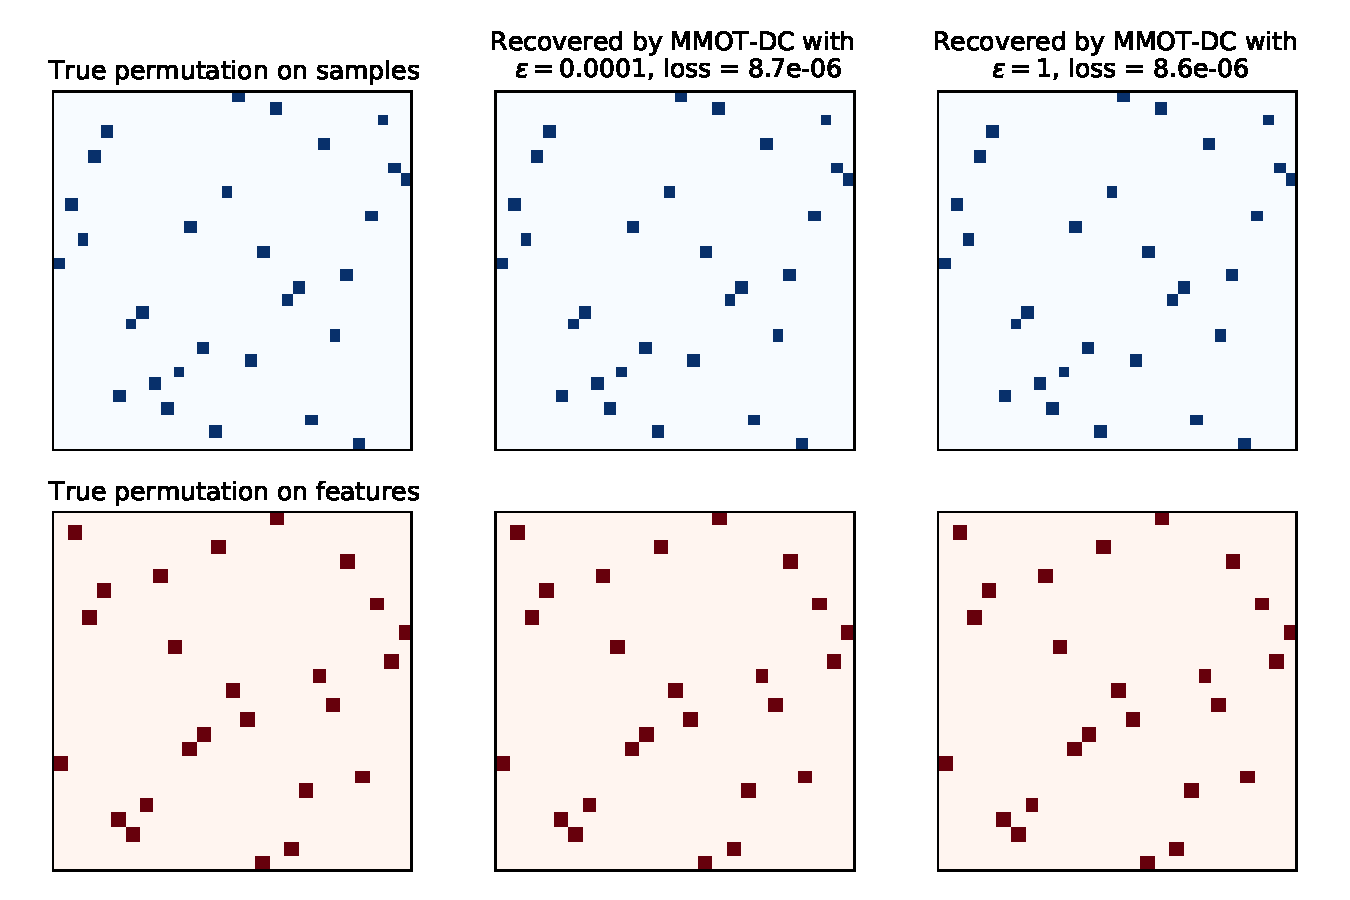
\includegraphics[width=0.8\textwidth,height=0.8\textheight,keepaspectratio]{./Chapitre2/fig/compare_methods.pdf}
  \caption{Couplings generated by COOT and MMOT-DC on the matrix recovering task.}
  \label{fig:permu}
\end{figure}
%%%%%%%%%%%%%%%%%%%%%%%%%%%%%%%%%%%%%%%
We also plot, with some abuse of notation, the histograms of the difference between
the $(1,3), (1,4), (2,3), (2,4)$-marginal matrices of MMOT-DC and their corresponding counterparts from F-MMOT.
In this example, in theory, as the optimal tensor $P$ of F-MMOT can be factorized as
$P = P_{\# \cT_1} \otimes P_{\# \cT_2} = Q_s \otimes Q_f$,
it is immediate to see that $P_{\# (1,3)} = P_{\# (1,4)} = P_{\# (2,3)} = P_{\# (2,4)} \in \bbR^{30 \times 25}$
are uniform matrices whose entries are $\frac{1}{750}$.
%%%%%%%%%%%%%%%%%%%%%%%%%%%%%%%%%%%%%%%
\begin{figure}[t]
  \centering
  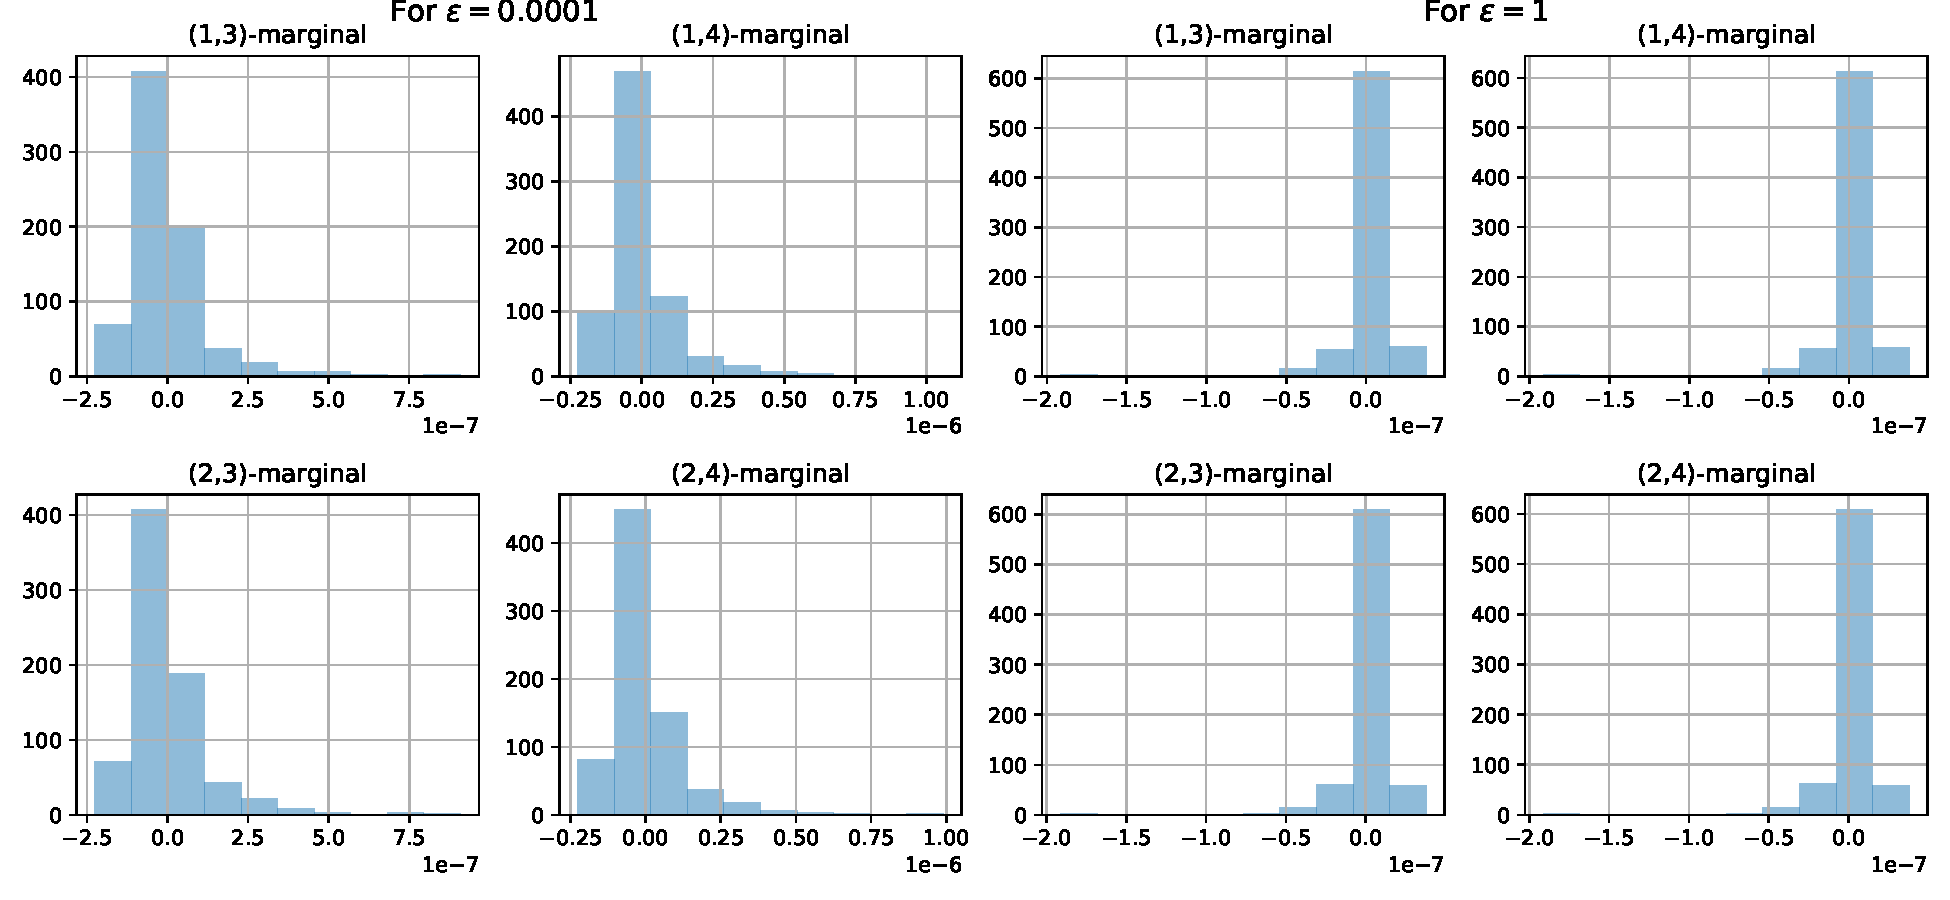
\includegraphics[width=1.\textwidth,height=1.\textheight,keepaspectratio]{./Chapitre2/fig/other_marginals.pdf}
  \caption{Histograms of difference between true independent marginal matrices and their approximations. We see that the marginal matrices obtained
  by \Cref{algo:dc_MMOT} approximate well the theoretical uniform matrices.}
  \label{fig:other_marg}
\end{figure}

%%%%%%%%%%%%%%%%%%%%%%%%%%%%%%%%%%%%%%%
\paragraph{Quality of the MMOT-DC solutions. \label{expe:2}}

% In the following example, our evaluation metric is the COOT loss $\langle C, P \otimes Q \rangle$,
% where the smaller the loss, the better.

Now, we consider the situation where the true matching between two matrices is not known in advance and investigate the quality
of the solutions returned by MMOT-DC to solve the COOT and GW problems. This means that we will look at the COOT loss
$\langle C, Q_s \otimes Q_f \rangle$, where the smaller the loss, the better when using both exact COOT and GW solvers
and our relaxation.

We generate two random matrices $X \in \bbR^{20 \times 3}$ and $Y \in \bbR^{30 \times 2}$,
whose entries are drawn independently from the uniform distribution on the interval $[0,1)$. Then we calculate two corresponding
squared Euclidean distance matrices of size $20$ and $30$. Their rows and columns are equipped with the discrete
uniform distributions. In this case, \citet{Redko20} show that the COOT loss coincides with the GW distance, and the
Block Coordinate Descent (BCD) algorithm used to approximate COOT is equivalent to the Frank-Wolfe algorithm \citep{Frank56}
used to solve the GW distance.

We compare four solvers:
\begin{enumerate}
  \item The Frank-Wolfe algorithm to solve the GW distance (GW-FW).

  \item The projected gradient algorithm to solve the entropic GW distance \citep{Peyre16} (EGW-PGD).
  We choose the regularization parameter from the set
  $\{0.0008, 0.0016, 0.0032, 0.0064, 0.0128, 0.0256 \}$
  and pick the one which corresponds to smallest COOT loss.

  \item The Block Coordinate Descent algorithm to approximate the entropic COOT \citep{Redko20}
  (EGW-BCD), where two additional KL divergences corresponding to two couplings are introduced.

  The regularization parameters are tuned from the set
  $\{0, 0.0005, 0.001, 0.005, 0.01, 0.05, 0.1, 0.5, 1 \}$,
  where $0$ means that there is no regularization term for the corresponding coupling
  and we pick the pair corresponding to the smallest COOT loss.

  \item \Cref{algo:dc_MMOT} to solve the MMOT-DC. We tune
  $\varepsilon \in \{1, 1.4, 1.8, 2.2, 2.6\}$ and we pick the one which corresponds to smallest COOT loss.
\end{enumerate}
For GW-FW and EGW-PGD, we use the implementation from the Python Optimal Transport package \citep{Flamary21}.

Given two random matrices, we record the COOT loss corresponding to the solution generated by each method.
We simulate this process $70$ times and compare their overall performance. We can see in \Cref{tab:gw} the average value and
standard deviation and the comparison for the values of the loss between the different algorithms in \Cref{fig:gw}.
The performance is quite similar across methods with a  slight advantage for EGW-PGD. This is in itself a very
interesting result that has never been noted, to the best of our knowledge: the reason that the entropic version of GW can
provide better solution than solving the exact problem, may be due to the "convexification" of the problem, thanks to the entropic
regularization. Our approach is also interestingly better than the exact GW-FW, which illustrates that the relaxation might help in
finding better solutions despite the non-convexity of the problem.
%%%%%%%%%%%%%%%%%%%%%%%%%%%%%%%%%%%%%%%
\begin{table}[t]
  % \vskip 0.15in
  \begin{center}
    \begin{small}
      \begin{sc}
        \begin{tabular}{|c|c|c|c|}
          \hline
          GW-FW & EGW-PGD & EGW-BCD & MMOT-DC \\
          \hline
          0.0829 ($\pm$ 0.0354) & \textbf{0.0786 ($\pm$ 0.0347)} & 0.0804 ($\pm$ 0.0353) & 0.0822 ($\pm$ 0.0364) \\
          \hline
        \end{tabular}
      \end{sc}
    \end{small}
  \end{center}
  \caption{Average and standard deviation of COOT loss of the solvers. MMOT-DC is competitive to other solvers,
  except for EGW-PGD and EGW-BCD.
  \label{tab:gw}}
\end{table}

%%%%%%%%%%%%%%%%%%%%%%%%%%%%%%%%%%%%%%%
\begin{figure}[t]
	\centering
	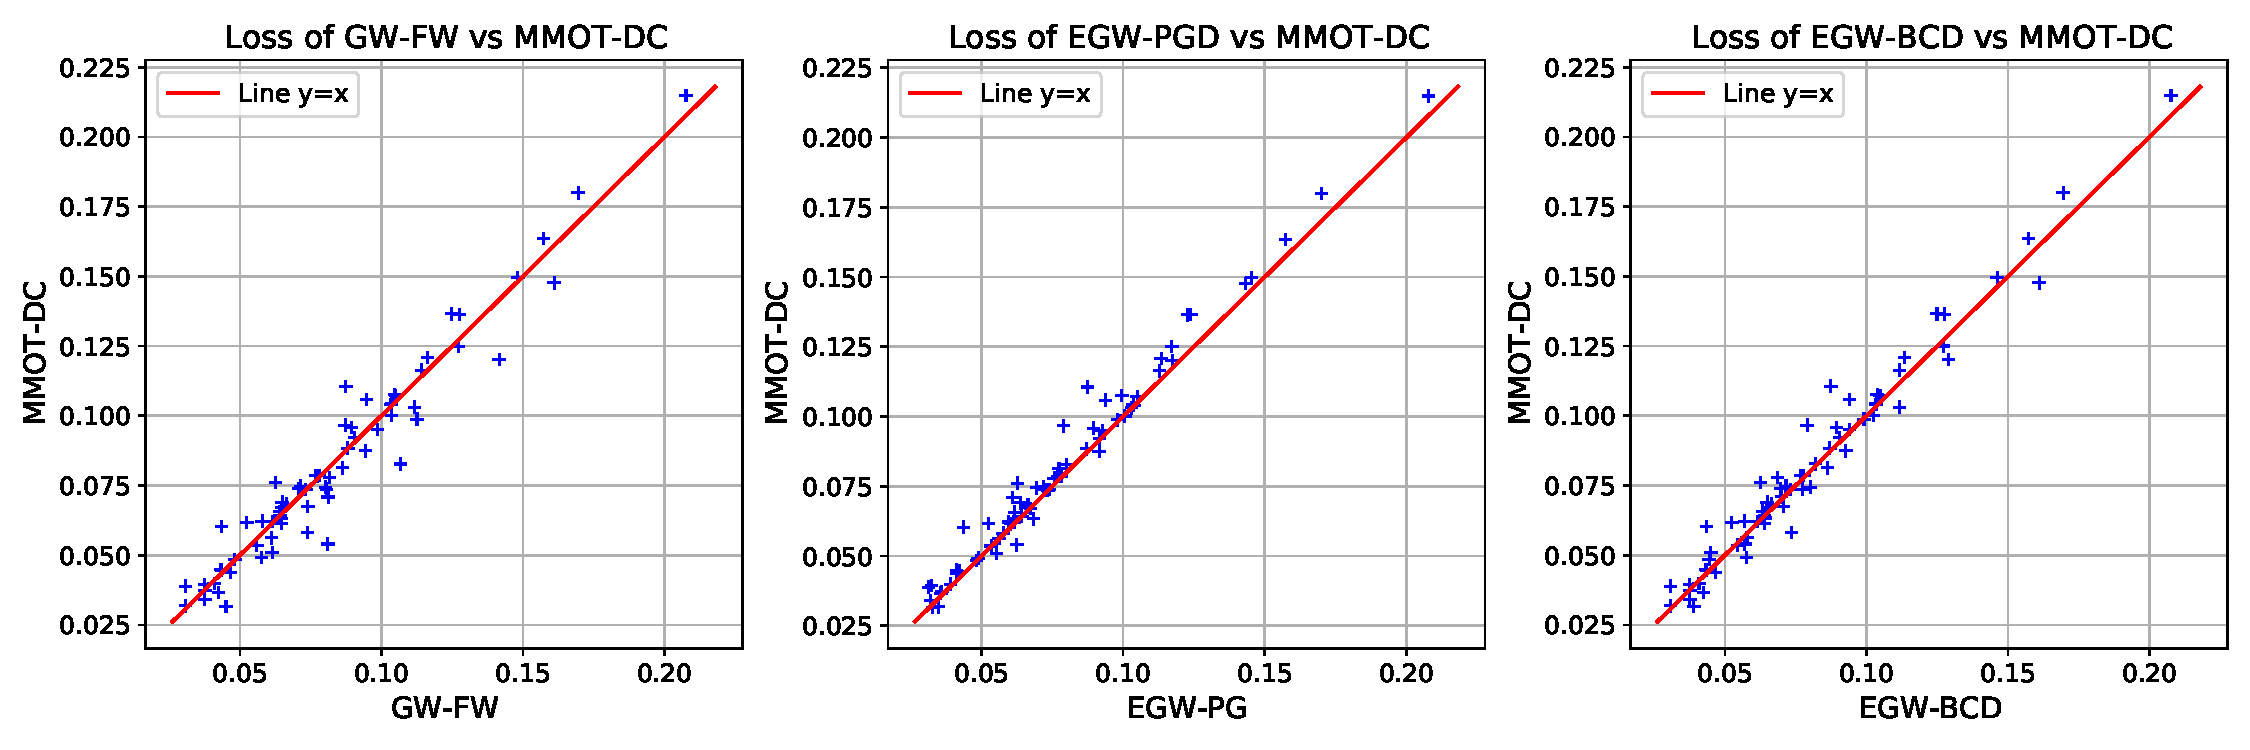
\includegraphics[width=\textwidth,height=\textheight,keepaspectratio]{./Chapitre2/fig/all_vs_MMOT-DC.pdf}
	\caption{Scatter plots of MMOT-DC versus other solvers. In all three plots, the points tend to concentrate around the line $y=x$,
  which indicates the comparable performance of MMOT-DC. On the other hand, the top-right plot shows the clear superiority of EGW-PGD.}
	\label{fig:gw}
\end{figure}
%%%%%%%%%%%%%%%%%%%%%%%%%%%%%%%%%%%%%%%

\paragraph{An empirical variation.} Intuitively, for sufficiently large $\varepsilon$, the minimisation of the KL divergence is prioritised
over the linear term in the objective function of the MMOT-DC problem, which implies that the optimal tensor $P^*$ is "close" to its
corresponding tensor product $P^*_{\# \cT}$. So, instead of calculating the gradient at $P$, one may calculate at
$P_{\# \cT}$. In this case, the gradient reads
\begin{equation}
  \begin{split}
    \sum_{m=1}^M \nabla_P \kl_m(P_{\# \cT}) =
    \log \frac{P_{\# \cT_1}}{\mu^{\otimes}_{\cT_1}} \oplus ... \oplus \log \frac{P_{\# \cT_m}}{\mu^{\otimes}_{\cT_m}} ,
  \end{split}
\end{equation}
where $\oplus$ represents the tensor sum operator between two arbitrary-size tensors: $(A \oplus B)_{i,j}:= A_i + B_j$, where with some
abuse of notation, $i$ or $j$ can be understood as a tuple of indices. Thus, we avoid storing the $N$-D gradient tensor (as in the
\Cref{algo:dc_MMOT}) and only need to store $M$ smaller-size tensors. Not only saving the memory,
this variation also seems to be empirically competitive with the original \Cref{algo:dc_MMOT}, if not sometimes better,
in terms of COOT loss. The underlying reason might be related to the approximate DCA scheme \citep{Thanh15}, where one replaces both
steps in each DC iteration by their approximation. We leave the formal theoretical justification of this variation to the future work.
We call this variation \textit{MMOT-DC-v1} and use the same setup as in Experiment \ref{expe:2}.
\begin{figure}[ht]
  \centering
  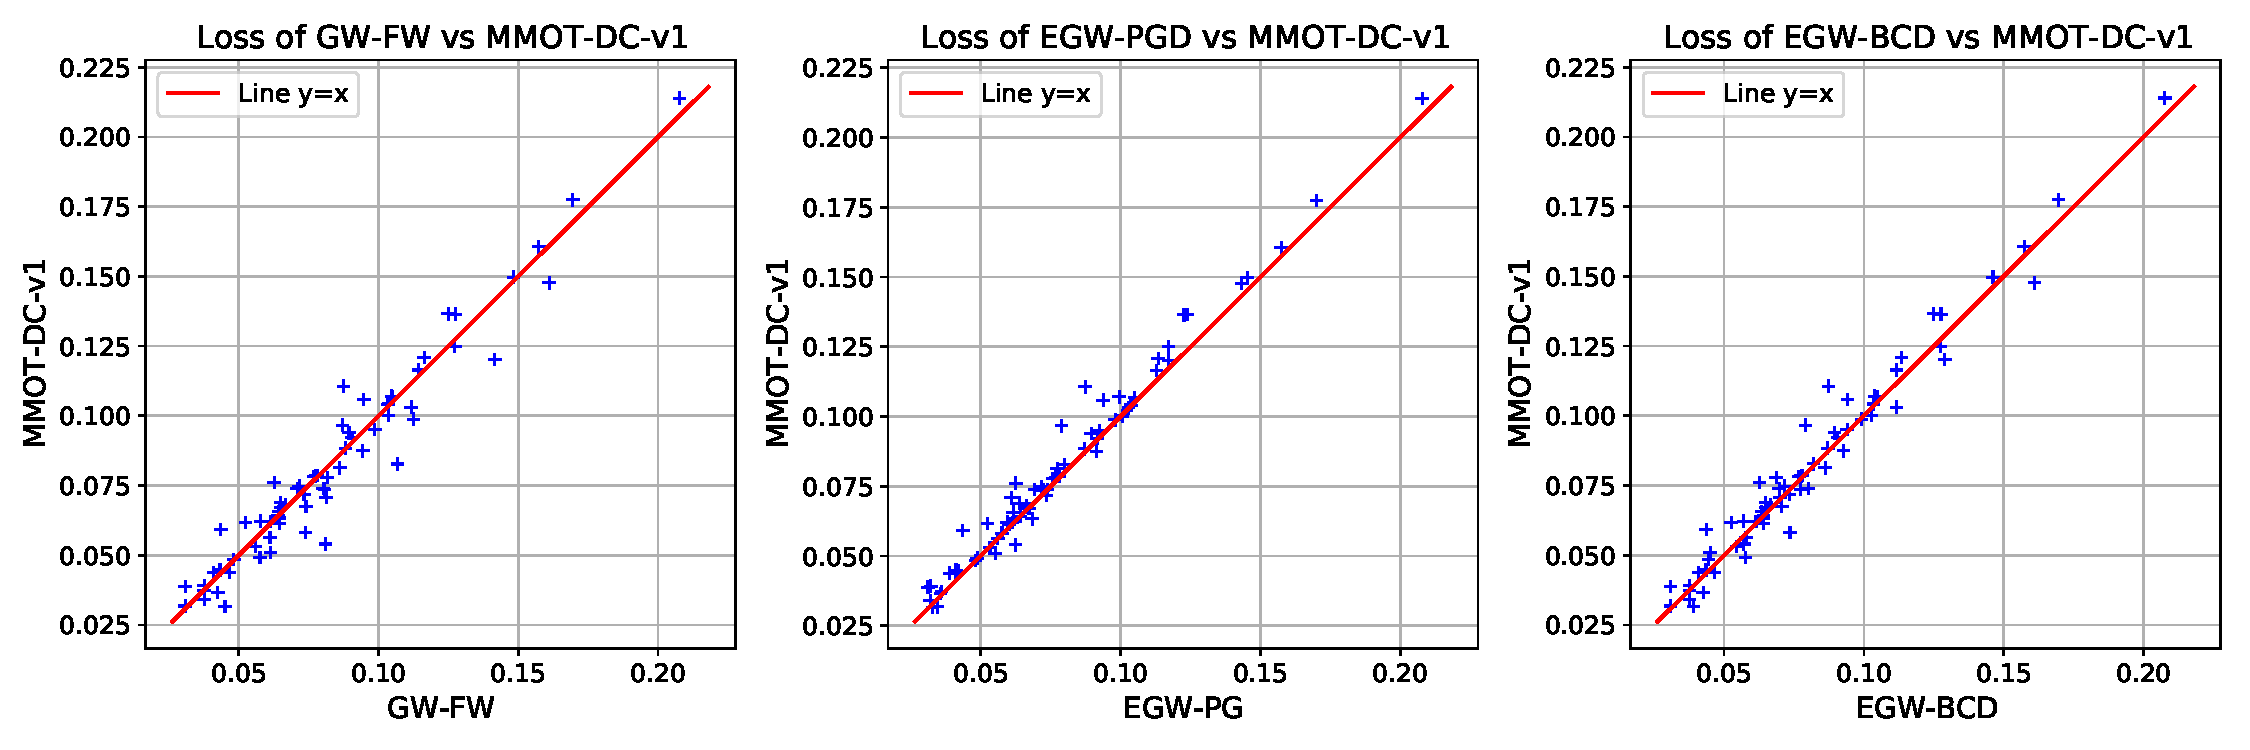
\includegraphics[width=\textwidth,height=\textheight,keepaspectratio]{./Chapitre2/fig/all_vs_MMOT-DC-v1.pdf}
  \caption{Scatter plots of MMOT-DC-v1 versus other solvers. In all three plots, the points tend to concentrate around the line $y=x$,
  which indicates the comparable performance of MMOT-DC-v1. On the other hand, the top-right plot shows the clear superiority of EGW-PGD.}
  \label{fig:coot_mmot_new}
\end{figure}

\begin{table}[H]
  \label{tab:coot_new}
  % \vskip 0.15in
  \begin{center}
    \begin{small}
      \begin{sc}
        \begin{tabular}{|c|c|}
          \hline
          MMOT-DC & MMOT-DC-v1 \\
          \hline
          0.0822 ($\pm$ 0.0364) & 0.0820 ($\pm$ 0.0361) \\
          \hline
        \end{tabular}
      \end{sc}
    \end{small}
  \end{center}
  \caption{Average and standard deviation of COOT loss of MMOT-DC and MMOT-DC-v1.
  The performance of the two algorithms is very similar.}
  % \vskip -0.1in
\end{table}

%%%%%%%%%%%%%%%%%%%%%%%%%%%%%%%%%%%%%%
\subsection{Conclusion and future work}
%%%%%%%%%%%%%%%%%%%%%%%%%%%%%%%%%%%%%%

In this section, we present a novel relaxation of the factorized MMOT problem called \textit{MMOT-DC}.
More precisely, we replace the
hard constraint on factorization constraint by a smooth regularization term. The resulting problem
not only enjoys an interpolation property between MMOT and factorized MMOT, but also is a DC problem,
which can be solved easily by the DC algorithm. We illustrate the use of MMOT-DC the via some simulated experiments and show that
it is competitive with the existing popular solvers of COOT and GW distance.
One limitation of the current DC algorithm is that, it is not scalable because
it requires storing a full-size tensor in the gradient step computation. Thus, future
work may focus on more efficiently designed algorithms, in terms of both time and memory footprint.
Moreover, incorporating additional structure on the cost tensor may also be computationally and practically beneficial.
From a theoretical viewpoint, it is also interesting to study the extension of MMOT-DC to the continuous setting,
which can potentially allow us to further understand the connection between GW distance and COOT.

% From a theoretical viewpoint, one potential application of MMOT-DC is on the study of the sample complexity of GW distance.
% More precisely, given two measure networks $\cX = (X, c_X, \mu_X)$ and $\cY = (Y, c_Y, \mu_Y)$,
% we want to quantify $| \gw(\cX, \cY) - \gw(\cX_n, \cY_n)|$. Note that, \citep{Zhang23} has also
% established the convergence rate for the case of $2$-GW distance, in which the cost function
% is the squared Euclidean distance. Our proposed approach, if works, would be able to handle any
% conditionally negative (or positive) semi-definite kernel.

% The idea is as follows: by \Cref{prop:coot_gw_equiv}, COOT and GW distance are equivalent
% \footnote{Note that one needs to properly extend \Cref{prop:coot_gw_equiv} to the continuous setting
% (of measure networks).}. So, we can replace GW by COOT, as it is less (unnecessarily) constrained.
% Next, we extend MMOT-DC to the continuous setting and show that the interpolation property
% still holds, notably MMOT-DC converges to COOT as regularization tends to the infinity.
% Thanks to the DC algo, we can linearize the MMOT-DC and obtain an entropic MMOT problem.
% This problem has two advantages. First, one can reuse the technique for entropic OT
% in \citep{Genevay19} and extend to the entropic MMOT. Second, for suitable choice of input,
% it approximates COOT.

% Note that, this is still an ongoing work as we have not yet fully resolved all
% technical difficulties. Nevertheless, we report the sketch of the proof and leave most of
% mathematical details in Appendix.

% \paragraph{Assumptions} We assume that the measure networks
% $\cX = (X, c_X, \mu_X)$ and $\cY = (Y, c_Y, \mu_Y)$. $X$ and $Y$ are compact
% subsets of $\bbR^{d_x}$ and $\bbR^{d_y}$, respectively. The probability measures
% $\mu_X$ and $\mu_Y$ are absolutely continuous with respect to the Lebesgue measures
% on $\bbR^{d_x}$ and $\bbR^{d_y}$, respectively.
% With some abuse of notation, we also use $\mu_X, \mu_Y$ to denote their density functions.

% \paragraph{Sketch of proof}
% For convenience, denote $\cU_4 = U(\mu_X, \mu_Y, \mu_X, \mu_Y)$ and $\mu = \mu_X \otimes \mu_Y$.
% We write $c = |c_X - c_Y|^2$ defined by $c(x, y, x', y') = |c_X(x, x') - c_Y(y, y') |^2$.
% Recall that, for any $\pi \in \cU_4$, we denote $\pi_{\#} = \pi_{\# 12} \otimes \pi_{\# 34}$.
% \begin{lemma}
%   For each $\pi \in \cU_4$, denote
%   $G(\pi) := \kl(\pi_{\# 12} | \mu) + \kl(\pi_{\# 34} | \mu) = \kl(\pi_{\#} | \mu^{\otimes 2})$.
%   Then $G$ is convex and differentiable. In particular, $G(\pi) = \int \nabla G(\pi) \; d \pi$,
%   for $\pi \in \cU_4$.
% \end{lemma}
% Now, we have
% \begin{align}
%   \int c \; d\gamma + \varepsilon \kl(\gamma | \gamma_{\#})
%   &\leq \int c \; d\gamma + \varepsilon \kl(\gamma | \mu^{\otimes 2})
%   - \varepsilon \Big[ G(\pi) + \int \nabla G(\pi) \; d \gamma - \int \nabla G(\pi) \; d \pi \Big] \\
%   &= \int \big[ c - \varepsilon \nabla G(\pi) \big] \; d \gamma
%   + \varepsilon \kl(\gamma | \mu^{\otimes 2}).
% \end{align}
% By taking infimum over $\cU_4$, we obtain
% \begin{align}
%   \mmotdc_{\varepsilon} \leq
%   \inf_{\gamma \in \cU_4} \int \big[ c - \varepsilon \nabla G(\pi) \big] d \gamma
%   + \varepsilon \kl(\gamma | \mu^{\otimes 2}).
% \end{align}
% Now, we define the following MMOT problem.
% \begin{definition}
%   For $\pi \in \cU_4$, define
%   \begin{align}
%     \mmot_{\varepsilon}\big( c - \varepsilon \nabla G(\pi) \big) :=
%     \inf_{\gamma \in \cU_4} \int \big[ c - \varepsilon \nabla G(\pi) \big] \; d \gamma
%       + \varepsilon \kl(\gamma | \mu^{\otimes 2}).
%   \end{align}
% \end{definition}
% There exists $\pi \in \cU_4$ such that $\mmot_{\varepsilon}\big( c - \varepsilon \nabla G(\pi) \big)$
% approximates COOT. For example, denote $\pi_{\varepsilon}$
% the solution of the entropic COOT problem $\coot_{\varepsilon}(\cX, \cY)$, we can show that
% \begin{corollary}
%   For every $\varepsilon > 0$, we have
%   $\coot_{1 / \varepsilon}(\cX, \cY) \geq
%   \mmot_{\varepsilon}\big( c - \varepsilon \nabla G(\pi_{1 / \varepsilon}) \big) \geq \mmotdc_{\varepsilon}$.
%   As a consequence,
%   $\mmot_{\varepsilon}\big( c - \varepsilon \nabla G(\pi_{1 / \varepsilon}) \big) \to \coot(\cX, \cY)$,
%   when $\varepsilon \to \infty$.
% \end{corollary}
% Now, suppose $\mmot_{\varepsilon}\big( c - \varepsilon \nabla G(\pi^*) \big)$ can approximate COOT,
% for some $\pi^* \in \cU_4$. Then, by the triangle inequality, we have
% \begin{align}
%   | \coot_(\cX, \cY) - \coot_(\cX_n, \cY_n)|
%   &\leq |\coot_(\cX, \cY) - \mmot_{\varepsilon}\big( c - \varepsilon \nabla G(\pi^*) \big)| \\
%   &+ |\mmot_{\varepsilon, n}\big( c - \varepsilon \nabla G(\pi^*) \big) - \mmot_{\varepsilon}\big( c - \varepsilon \nabla G(\pi^*) \big)| \\
%   &+ |\coot(\cX_n, \cY_n) - \mmot_{\varepsilon, n}\big( c - \varepsilon \nabla G(\pi^*) \big)|,
% \end{align}
% Now, it is enough to bound each term and obtain the final rate. However, the main difficulties
% lie on finding the appropriate choice of $\pi^*$ and on how to control
% it in the entropic MMOT problem.

% \subsection{Stability of Co-Optimal Transport}

% COOT setting: given two sample-feature spaces
% $\cX_1 = ((X_1^s, \mu_1^s), (X_1^f, \mu_1^f), \xi_1)$ and
% $\cX_2 = ((X_2^s, \mu_2^s), (X_2^f, \mu_2^f), \xi_2)$. COOT reads
% \begin{equation}
%     \coot(\cX_1, \cX_2) =
%     \inf_{\substack{\pi^s \in U() \\ \pi^f \in U()}}
%     \int |\xi_1 - \xi_2|^2 d\pi^s d\pi^f
% \end{equation}
% Consider the "semi-empirical" spaces:
% $\widehat{\cX}_i := ((\widehat{X}_i^s, \widehat{\mu}_i^s), (X_i^f, \mu_i^f), \xi_i))$, where
% we fix the dimension $f$ and only consider the empirical version of sample measures.
% Now, how does the feature coupling behave when $\widehat{\mu}^s \to \mu^s$?, i.e. when $n \to \infty$,
% quantify
% \begin{equation}
%     | \coot(\cX_1, \cX_2) -
%     \coot(\widehat{\cX}_1, \widehat{\cX}_2) |
% \end{equation}
% We can first start with finite-dimensional feature spaces (so the feature coupling is a matrix).

\vfill
% }

\clearemptydoublepage
\backmatter

% Chapitre pour la bibliographie
% Bibliography chapter
\clearemptydoublepage
\phantomsection % To have a correct link in the table of contents
\addcontentsline{toc}{chapter}{Bibliography}
\nocite{*}
\printbibliography{}

% nocite: Pour citer la totalit\'{e} des r\'{e}f\'{e}rences contenues dans le fichier biblio
% nocite: In order to cite all the references included biblio% \nocite{*}
% \nocite{*}
% \printbibliography[heading=primary,keyword=primary]
% \newpage
% \nocite{*}
% \printbibliography[heading=secondary,keyword=secondary]

% Pour avoir la quatrième de couverture sur une page paire
% To have the back cover on an even page
\cleartoevenpage[\thispagestyle{empty}]
\markboth{}{}
% Plus petite marge du bas pour la quatrième de couverture
% Shorter bottom margin for the back cover
\newgeometry{inner=30mm,outer=20mm,top=40mm,bottom=20mm}

%insertion de l'image de fond du dos (resume)
%background image for resume (back)
\backcoverheader

% Switch font style to back cover style
\selectfontbackcover{ % Font style change is limited to this page using braces, just in case

\titleFR{Transport optimal pour l'apprentissage par transfert entre les espaces}

\keywordsFR{Transport Optimal Non-équilibré, Gromov-Wasserstein, Co-Optimal Transport,
Adaptation de Domaine Hétérogène}

\abstractFR{Au cours des dernières années, la remarquable puissance de la théorie du transport optimal
a largement dépassé la comparaison classique des mesures de probabilité évoluant dans le même espace sous-jacent.
Dans cette thèse, nous nous intéressons aux problèmes de transport optimal
entre des espaces incomparables. Plus précisément, nous nous concentrons sur la relaxation marginale
du transport optimal (équilibré) de Gromov-Wasserstein et du Co-Optimal Transport,
ainsi que sur l'intégration de connaissances préalables dans la distance de Gromov-Wasserstein et
sa formulation non-équilibrée. Nous commençons par le Co-Optimal Transport en cadre continu,
qui sert de première étape vers l'étude de l'approximation entropique et
de l'extension non-équilibrée. Ensuite, nous introduisons la formulation non-équilibrée du Co-Optimal Transport
et montrons sa robustesse aux valeurs aberrantes, contrairement à son homologue équilibré. Ensuite,
nous proposons d'utiliser la divergence de Fused Gromov-Wasserstein non-équilibrée
pour aligner les surfaces corticales,
en exploitant simultanément les signaux fonctionnels et la structure anatomique du cerveau humain.
Enfin, nous renforçons davantage la distance de Gromov-Wasserstein avec la capacité de
manipuler plus efficacement les données brutes et d'effectuer un appariement des features génomiques.}

\titleEN{Optimal transport for transfer learning across domains}

\keywordsEN{Unbalanced Optimal Transport, Gromov-Wasserstein, Co-Optimal Transport,
Heterogeneous Domain Adaptation}

\abstractEN{In the recent years, the remarkable versatility of optimal transport theory
has gone far beyond the classic comparison of the probability measures living in the same underlying space.
In this thesis, we are interested in the optimal transport problems
between incomparable spaces. More precisely, we focus on the marginal relaxation of the (balanced)
Gromov-Wasserstein and Co-Optimal Transport,
as well as the integration of prior knownledge into Gromov-Wasserstein distance and
its unbalanced formulation. We start with the Co-Optimal Transport in continuous setting,
which serves as the first step towards the study of the entropic approximation and
unbalanced extension. Then, we introduce the unbalanced formulation of the Co-Optimal Transport
and show its robustness to outliers, by contrast to the balanced counterpart. Next,
we propose to use the fused unbalanced Gromov-Wasserstein divergence to align the cortical surfaces,
by simultaneously exploiting the functional signals and anatomical structure of human brain.
Finally, we further empower the Gromov-Wasserstein distance with the ability to
manipulate more efficiently the input data and to perform meaningful genomic feature matching.}

}

% Rétablit les marges d'origines
% Restore original margin settings
\restoregeometry


\end{document}
